\documentclass[twoside]{book}

% Packages required by doxygen
\usepackage{calc}
\usepackage{doxygen}
\usepackage{graphicx}
\usepackage[utf8]{inputenc}
\usepackage{makeidx}
\usepackage{multicol}
\usepackage{multirow}
\usepackage{textcomp}
\usepackage[table]{xcolor}

% Font selection
\usepackage[T1]{fontenc}
\usepackage{mathptmx}
\usepackage[scaled=.90]{helvet}
\usepackage{courier}
\usepackage{amssymb}
\usepackage{sectsty}
\renewcommand{\familydefault}{\sfdefault}
\allsectionsfont{%
  \fontseries{bc}\selectfont%
  \color{darkgray}%
}
\renewcommand{\DoxyLabelFont}{%
  \fontseries{bc}\selectfont%
  \color{darkgray}%
}

% Page & text layout
\usepackage{geometry}
\geometry{%
  a4paper,%
  top=2.5cm,%
  bottom=2.5cm,%
  left=2.5cm,%
  right=2.5cm%
}
\tolerance=750
\hfuzz=15pt
\hbadness=750
\setlength{\emergencystretch}{15pt}
\setlength{\parindent}{0cm}
\setlength{\parskip}{0.2cm}
\makeatletter
\renewcommand{\paragraph}{%
  \@startsection{paragraph}{4}{0ex}{-1.0ex}{1.0ex}{%
    \normalfont\normalsize\bfseries\SS@parafont%
  }%
}
\renewcommand{\subparagraph}{%
  \@startsection{subparagraph}{5}{0ex}{-1.0ex}{1.0ex}{%
    \normalfont\normalsize\bfseries\SS@subparafont%
  }%
}
\makeatother

% Headers & footers
\usepackage{fancyhdr}
\pagestyle{fancyplain}
\fancyhead[LE]{\fancyplain{}{\bfseries\thepage}}
\fancyhead[CE]{\fancyplain{}{}}
\fancyhead[RE]{\fancyplain{}{\bfseries\leftmark}}
\fancyhead[LO]{\fancyplain{}{\bfseries\rightmark}}
\fancyhead[CO]{\fancyplain{}{}}
\fancyhead[RO]{\fancyplain{}{\bfseries\thepage}}
\fancyfoot[LE]{\fancyplain{}{}}
\fancyfoot[CE]{\fancyplain{}{}}
\fancyfoot[RE]{\fancyplain{}{\bfseries\scriptsize Generated on Sun Sep 7 2014 22\-:10\-:00 for xv6 by Doxygen }}
\fancyfoot[LO]{\fancyplain{}{\bfseries\scriptsize Generated on Sun Sep 7 2014 22\-:10\-:00 for xv6 by Doxygen }}
\fancyfoot[CO]{\fancyplain{}{}}
\fancyfoot[RO]{\fancyplain{}{}}
\renewcommand{\footrulewidth}{0.4pt}
\renewcommand{\chaptermark}[1]{%
  \markboth{#1}{}%
}
\renewcommand{\sectionmark}[1]{%
  \markright{\thesection\ #1}%
}

% Indices & bibliography
\usepackage{natbib}
\usepackage[titles]{tocloft}
\setcounter{tocdepth}{3}
\setcounter{secnumdepth}{5}
\makeindex

% Hyperlinks (required, but should be loaded last)
\usepackage{ifpdf}
\ifpdf
  \usepackage[pdftex,pagebackref=true]{hyperref}
\else
  \usepackage[ps2pdf,pagebackref=true]{hyperref}
\fi
\hypersetup{%
  colorlinks=true,%
  linkcolor=blue,%
  citecolor=blue,%
  unicode%
}

% Custom commands
\newcommand{\clearemptydoublepage}{%
  \newpage{\pagestyle{empty}\cleardoublepage}%
}


%===== C O N T E N T S =====

\begin{document}

% Titlepage & ToC
\hypersetup{pageanchor=false}
\pagenumbering{roman}
\begin{titlepage}
\vspace*{7cm}
\begin{center}%
{\Large xv6 }\\
\vspace*{1cm}
{\large Generated by Doxygen 1.8.6}\\
\vspace*{0.5cm}
{\small Sun Sep 7 2014 22:10:00}\\
\end{center}
\end{titlepage}
\clearemptydoublepage
\tableofcontents
\clearemptydoublepage
\pagenumbering{arabic}
\hypersetup{pageanchor=true}

%--- Begin generated contents ---
\chapter{xv6}
\label{md__r_e_a_d_m_e}
\hypertarget{md__r_e_a_d_m_e}{}
A modification of the original xv6 os code 
\chapter{Data Structure Index}
\section{Data Structures}
Here are the data structures with brief descriptions\-:\begin{DoxyCompactList}
\item\contentsline{section}{\hyperlink{structbackcmd}{backcmd} }{\pageref{structbackcmd}}{}
\item\contentsline{section}{\hyperlink{structbuf}{buf} }{\pageref{structbuf}}{}
\item\contentsline{section}{\hyperlink{structcmd}{cmd} }{\pageref{structcmd}}{}
\item\contentsline{section}{\hyperlink{structcontext}{context} }{\pageref{structcontext}}{}
\item\contentsline{section}{\hyperlink{structcpu}{cpu} }{\pageref{structcpu}}{}
\item\contentsline{section}{\hyperlink{structdevsw}{devsw} }{\pageref{structdevsw}}{}
\item\contentsline{section}{\hyperlink{structdinode}{dinode} }{\pageref{structdinode}}{}
\item\contentsline{section}{\hyperlink{structdirent}{dirent} }{\pageref{structdirent}}{}
\item\contentsline{section}{\hyperlink{structelfhdr}{elfhdr} }{\pageref{structelfhdr}}{}
\item\contentsline{section}{\hyperlink{structexeccmd}{execcmd} }{\pageref{structexeccmd}}{}
\item\contentsline{section}{\hyperlink{structfile}{file} }{\pageref{structfile}}{}
\item\contentsline{section}{\hyperlink{structgatedesc}{gatedesc} }{\pageref{structgatedesc}}{}
\item\contentsline{section}{\hyperlink{unionheader}{header} }{\pageref{unionheader}}{}
\item\contentsline{section}{\hyperlink{structinode}{inode} }{\pageref{structinode}}{}
\item\contentsline{section}{\hyperlink{structioapic}{ioapic} }{\pageref{structioapic}}{}
\item\contentsline{section}{\hyperlink{structlistcmd}{listcmd} }{\pageref{structlistcmd}}{}
\item\contentsline{section}{\hyperlink{structmp}{mp} }{\pageref{structmp}}{}
\item\contentsline{section}{\hyperlink{structmpconf}{mpconf} }{\pageref{structmpconf}}{}
\item\contentsline{section}{\hyperlink{structmpioapic}{mpioapic} }{\pageref{structmpioapic}}{}
\item\contentsline{section}{\hyperlink{structmpproc}{mpproc} }{\pageref{structmpproc}}{}
\item\contentsline{section}{\hyperlink{structpipe}{pipe} }{\pageref{structpipe}}{}
\item\contentsline{section}{\hyperlink{structpipecmd}{pipecmd} }{\pageref{structpipecmd}}{}
\item\contentsline{section}{\hyperlink{structproc}{proc} }{\pageref{structproc}}{}
\item\contentsline{section}{\hyperlink{structproghdr}{proghdr} }{\pageref{structproghdr}}{}
\item\contentsline{section}{\hyperlink{structredircmd}{redircmd} }{\pageref{structredircmd}}{}
\item\contentsline{section}{\hyperlink{structrun}{run} }{\pageref{structrun}}{}
\item\contentsline{section}{\hyperlink{structsegdesc}{segdesc} }{\pageref{structsegdesc}}{}
\item\contentsline{section}{\hyperlink{structspinlock}{spinlock} }{\pageref{structspinlock}}{}
\item\contentsline{section}{\hyperlink{structstat}{stat} }{\pageref{structstat}}{}
\item\contentsline{section}{\hyperlink{structsuperblock}{superblock} }{\pageref{structsuperblock}}{}
\item\contentsline{section}{\hyperlink{structtaskstate}{taskstate} }{\pageref{structtaskstate}}{}
\item\contentsline{section}{\hyperlink{structtrapframe}{trapframe} }{\pageref{structtrapframe}}{}
\end{DoxyCompactList}

\chapter{File Index}
\section{File List}
Here is a list of all files with brief descriptions\-:\begin{DoxyCompactList}
\item\contentsline{section}{include/\hyperlink{fcntl_8h}{fcntl.\-h} }{\pageref{fcntl_8h}}{}
\item\contentsline{section}{include/\hyperlink{fs_8h}{fs.\-h} }{\pageref{fs_8h}}{}
\item\contentsline{section}{include/\hyperlink{param_8h}{param.\-h} }{\pageref{param_8h}}{}
\item\contentsline{section}{include/\hyperlink{stat_8h}{stat.\-h} }{\pageref{stat_8h}}{}
\item\contentsline{section}{include/\hyperlink{syscall_8h}{syscall.\-h} }{\pageref{syscall_8h}}{}
\item\contentsline{section}{include/\hyperlink{traps_8h}{traps.\-h} }{\pageref{traps_8h}}{}
\item\contentsline{section}{include/\hyperlink{types_8h}{types.\-h} }{\pageref{types_8h}}{}
\item\contentsline{section}{include/\hyperlink{x86_8h}{x86.\-h} }{\pageref{x86_8h}}{}
\item\contentsline{section}{kernel/\hyperlink{asm_8h}{asm.\-h} }{\pageref{asm_8h}}{}
\item\contentsline{section}{kernel/\hyperlink{bio_8c}{bio.\-c} }{\pageref{bio_8c}}{}
\item\contentsline{section}{kernel/\hyperlink{bio_8d}{bio.\-d} }{\pageref{bio_8d}}{}
\item\contentsline{section}{kernel/\hyperlink{bootasm_8d}{bootasm.\-d} }{\pageref{bootasm_8d}}{}
\item\contentsline{section}{kernel/\hyperlink{bootmain_8c}{bootmain.\-c} }{\pageref{bootmain_8c}}{}
\item\contentsline{section}{kernel/\hyperlink{bootmain_8d}{bootmain.\-d} }{\pageref{bootmain_8d}}{}
\item\contentsline{section}{kernel/\hyperlink{bootother_8d}{bootother.\-d} }{\pageref{bootother_8d}}{}
\item\contentsline{section}{kernel/\hyperlink{buf_8h}{buf.\-h} }{\pageref{buf_8h}}{}
\item\contentsline{section}{kernel/\hyperlink{console_8c}{console.\-c} }{\pageref{console_8c}}{}
\item\contentsline{section}{kernel/\hyperlink{console_8d}{console.\-d} }{\pageref{console_8d}}{}
\item\contentsline{section}{kernel/\hyperlink{data_8d}{data.\-d} }{\pageref{data_8d}}{}
\item\contentsline{section}{kernel/\hyperlink{defs_8h}{defs.\-h} }{\pageref{defs_8h}}{}
\item\contentsline{section}{kernel/\hyperlink{elf_8h}{elf.\-h} }{\pageref{elf_8h}}{}
\item\contentsline{section}{kernel/\hyperlink{exec_8c}{exec.\-c} }{\pageref{exec_8c}}{}
\item\contentsline{section}{kernel/\hyperlink{exec_8d}{exec.\-d} }{\pageref{exec_8d}}{}
\item\contentsline{section}{kernel/\hyperlink{file_8c}{file.\-c} }{\pageref{file_8c}}{}
\item\contentsline{section}{kernel/\hyperlink{file_8d}{file.\-d} }{\pageref{file_8d}}{}
\item\contentsline{section}{kernel/\hyperlink{file_8h}{file.\-h} }{\pageref{file_8h}}{}
\item\contentsline{section}{kernel/\hyperlink{fs_8c}{fs.\-c} }{\pageref{fs_8c}}{}
\item\contentsline{section}{kernel/\hyperlink{fs_8d}{fs.\-d} }{\pageref{fs_8d}}{}
\item\contentsline{section}{kernel/\hyperlink{ide_8c}{ide.\-c} }{\pageref{ide_8c}}{}
\item\contentsline{section}{kernel/\hyperlink{ide_8d}{ide.\-d} }{\pageref{ide_8d}}{}
\item\contentsline{section}{kernel/\hyperlink{initcode_8d}{initcode.\-d} }{\pageref{initcode_8d}}{}
\item\contentsline{section}{kernel/\hyperlink{ioapic_8c}{ioapic.\-c} }{\pageref{ioapic_8c}}{}
\item\contentsline{section}{kernel/\hyperlink{ioapic_8d}{ioapic.\-d} }{\pageref{ioapic_8d}}{}
\item\contentsline{section}{kernel/\hyperlink{kalloc_8c}{kalloc.\-c} }{\pageref{kalloc_8c}}{}
\item\contentsline{section}{kernel/\hyperlink{kalloc_8d}{kalloc.\-d} }{\pageref{kalloc_8d}}{}
\item\contentsline{section}{kernel/\hyperlink{kbd_8c}{kbd.\-c} }{\pageref{kbd_8c}}{}
\item\contentsline{section}{kernel/\hyperlink{kbd_8d}{kbd.\-d} }{\pageref{kbd_8d}}{}
\item\contentsline{section}{kernel/\hyperlink{kbd_8h}{kbd.\-h} }{\pageref{kbd_8h}}{}
\item\contentsline{section}{kernel/\hyperlink{lapic_8c}{lapic.\-c} }{\pageref{lapic_8c}}{}
\item\contentsline{section}{kernel/\hyperlink{lapic_8d}{lapic.\-d} }{\pageref{lapic_8d}}{}
\item\contentsline{section}{kernel/\hyperlink{main_8c}{main.\-c} }{\pageref{main_8c}}{}
\item\contentsline{section}{kernel/\hyperlink{main_8d}{main.\-d} }{\pageref{main_8d}}{}
\item\contentsline{section}{kernel/\hyperlink{mmu_8h}{mmu.\-h} }{\pageref{mmu_8h}}{}
\item\contentsline{section}{kernel/\hyperlink{mp_8c}{mp.\-c} }{\pageref{mp_8c}}{}
\item\contentsline{section}{kernel/\hyperlink{mp_8d}{mp.\-d} }{\pageref{mp_8d}}{}
\item\contentsline{section}{kernel/\hyperlink{mp_8h}{mp.\-h} }{\pageref{mp_8h}}{}
\item\contentsline{section}{kernel/\hyperlink{multiboot_8d}{multiboot.\-d} }{\pageref{multiboot_8d}}{}
\item\contentsline{section}{kernel/\hyperlink{picirq_8c}{picirq.\-c} }{\pageref{picirq_8c}}{}
\item\contentsline{section}{kernel/\hyperlink{picirq_8d}{picirq.\-d} }{\pageref{picirq_8d}}{}
\item\contentsline{section}{kernel/\hyperlink{pipe_8c}{pipe.\-c} }{\pageref{pipe_8c}}{}
\item\contentsline{section}{kernel/\hyperlink{pipe_8d}{pipe.\-d} }{\pageref{pipe_8d}}{}
\item\contentsline{section}{kernel/\hyperlink{proc_8c}{proc.\-c} }{\pageref{proc_8c}}{}
\item\contentsline{section}{kernel/\hyperlink{proc_8d}{proc.\-d} }{\pageref{proc_8d}}{}
\item\contentsline{section}{kernel/\hyperlink{proc_8h}{proc.\-h} }{\pageref{proc_8h}}{}
\item\contentsline{section}{kernel/\hyperlink{spinlock_8c}{spinlock.\-c} }{\pageref{spinlock_8c}}{}
\item\contentsline{section}{kernel/\hyperlink{spinlock_8d}{spinlock.\-d} }{\pageref{spinlock_8d}}{}
\item\contentsline{section}{kernel/\hyperlink{spinlock_8h}{spinlock.\-h} }{\pageref{spinlock_8h}}{}
\item\contentsline{section}{kernel/\hyperlink{string_8c}{string.\-c} }{\pageref{string_8c}}{}
\item\contentsline{section}{kernel/\hyperlink{string_8d}{string.\-d} }{\pageref{string_8d}}{}
\item\contentsline{section}{kernel/\hyperlink{swtch_8d}{swtch.\-d} }{\pageref{swtch_8d}}{}
\item\contentsline{section}{kernel/\hyperlink{syscall_8c}{syscall.\-c} }{\pageref{syscall_8c}}{}
\item\contentsline{section}{kernel/\hyperlink{syscall_8d}{syscall.\-d} }{\pageref{syscall_8d}}{}
\item\contentsline{section}{kernel/\hyperlink{sysfile_8c}{sysfile.\-c} }{\pageref{sysfile_8c}}{}
\item\contentsline{section}{kernel/\hyperlink{sysfile_8d}{sysfile.\-d} }{\pageref{sysfile_8d}}{}
\item\contentsline{section}{kernel/\hyperlink{sysfunc_8h}{sysfunc.\-h} }{\pageref{sysfunc_8h}}{}
\item\contentsline{section}{kernel/\hyperlink{sysproc_8c}{sysproc.\-c} }{\pageref{sysproc_8c}}{}
\item\contentsline{section}{kernel/\hyperlink{sysproc_8d}{sysproc.\-d} }{\pageref{sysproc_8d}}{}
\item\contentsline{section}{kernel/\hyperlink{timer_8c}{timer.\-c} }{\pageref{timer_8c}}{}
\item\contentsline{section}{kernel/\hyperlink{timer_8d}{timer.\-d} }{\pageref{timer_8d}}{}
\item\contentsline{section}{kernel/\hyperlink{trap_8c}{trap.\-c} }{\pageref{trap_8c}}{}
\item\contentsline{section}{kernel/\hyperlink{trap_8d}{trap.\-d} }{\pageref{trap_8d}}{}
\item\contentsline{section}{kernel/\hyperlink{trapasm_8d}{trapasm.\-d} }{\pageref{trapasm_8d}}{}
\item\contentsline{section}{kernel/\hyperlink{uart_8c}{uart.\-c} }{\pageref{uart_8c}}{}
\item\contentsline{section}{kernel/\hyperlink{uart_8d}{uart.\-d} }{\pageref{uart_8d}}{}
\item\contentsline{section}{kernel/\hyperlink{vectors_8d}{vectors.\-d} }{\pageref{vectors_8d}}{}
\item\contentsline{section}{kernel/\hyperlink{vm_8c}{vm.\-c} }{\pageref{vm_8c}}{}
\item\contentsline{section}{kernel/\hyperlink{vm_8d}{vm.\-d} }{\pageref{vm_8d}}{}
\item\contentsline{section}{tools/\hyperlink{mkfs_8c}{mkfs.\-c} }{\pageref{mkfs_8c}}{}
\item\contentsline{section}{tools/\hyperlink{mkfs_8d}{mkfs.\-d} }{\pageref{mkfs_8d}}{}
\item\contentsline{section}{user/\hyperlink{andrew_8c}{andrew.\-c} }{\pageref{andrew_8c}}{}
\item\contentsline{section}{user/\hyperlink{andrew_8d}{andrew.\-d} }{\pageref{andrew_8d}}{}
\item\contentsline{section}{user/\hyperlink{cat_8c}{cat.\-c} }{\pageref{cat_8c}}{}
\item\contentsline{section}{user/\hyperlink{cat_8d}{cat.\-d} }{\pageref{cat_8d}}{}
\item\contentsline{section}{user/\hyperlink{echo_8c}{echo.\-c} }{\pageref{echo_8c}}{}
\item\contentsline{section}{user/\hyperlink{echo_8d}{echo.\-d} }{\pageref{echo_8d}}{}
\item\contentsline{section}{user/\hyperlink{forktest_8c}{forktest.\-c} }{\pageref{forktest_8c}}{}
\item\contentsline{section}{user/\hyperlink{forktest_8d}{forktest.\-d} }{\pageref{forktest_8d}}{}
\item\contentsline{section}{user/\hyperlink{grep_8c}{grep.\-c} }{\pageref{grep_8c}}{}
\item\contentsline{section}{user/\hyperlink{grep_8d}{grep.\-d} }{\pageref{grep_8d}}{}
\item\contentsline{section}{user/\hyperlink{init_8c}{init.\-c} }{\pageref{init_8c}}{}
\item\contentsline{section}{user/\hyperlink{init_8d}{init.\-d} }{\pageref{init_8d}}{}
\item\contentsline{section}{user/\hyperlink{kill_8c}{kill.\-c} }{\pageref{kill_8c}}{}
\item\contentsline{section}{user/\hyperlink{kill_8d}{kill.\-d} }{\pageref{kill_8d}}{}
\item\contentsline{section}{user/\hyperlink{ln_8c}{ln.\-c} }{\pageref{ln_8c}}{}
\item\contentsline{section}{user/\hyperlink{ln_8d}{ln.\-d} }{\pageref{ln_8d}}{}
\item\contentsline{section}{user/\hyperlink{ls_8c}{ls.\-c} }{\pageref{ls_8c}}{}
\item\contentsline{section}{user/\hyperlink{ls_8d}{ls.\-d} }{\pageref{ls_8d}}{}
\item\contentsline{section}{user/\hyperlink{mkdir_8c}{mkdir.\-c} }{\pageref{mkdir_8c}}{}
\item\contentsline{section}{user/\hyperlink{mkdir_8d}{mkdir.\-d} }{\pageref{mkdir_8d}}{}
\item\contentsline{section}{user/\hyperlink{printf_8c}{printf.\-c} }{\pageref{printf_8c}}{}
\item\contentsline{section}{user/\hyperlink{printf_8d}{printf.\-d} }{\pageref{printf_8d}}{}
\item\contentsline{section}{user/\hyperlink{rm_8c}{rm.\-c} }{\pageref{rm_8c}}{}
\item\contentsline{section}{user/\hyperlink{rm_8d}{rm.\-d} }{\pageref{rm_8d}}{}
\item\contentsline{section}{user/\hyperlink{sh_8c}{sh.\-c} }{\pageref{sh_8c}}{}
\item\contentsline{section}{user/\hyperlink{sh_8d}{sh.\-d} }{\pageref{sh_8d}}{}
\item\contentsline{section}{user/\hyperlink{stressfs_8c}{stressfs.\-c} }{\pageref{stressfs_8c}}{}
\item\contentsline{section}{user/\hyperlink{stressfs_8d}{stressfs.\-d} }{\pageref{stressfs_8d}}{}
\item\contentsline{section}{user/\hyperlink{tester_8c}{tester.\-c} }{\pageref{tester_8c}}{}
\item\contentsline{section}{user/\hyperlink{tester_8d}{tester.\-d} }{\pageref{tester_8d}}{}
\item\contentsline{section}{user/\hyperlink{ulib_8c}{ulib.\-c} }{\pageref{ulib_8c}}{}
\item\contentsline{section}{user/\hyperlink{ulib_8d}{ulib.\-d} }{\pageref{ulib_8d}}{}
\item\contentsline{section}{user/\hyperlink{umalloc_8c}{umalloc.\-c} }{\pageref{umalloc_8c}}{}
\item\contentsline{section}{user/\hyperlink{umalloc_8d}{umalloc.\-d} }{\pageref{umalloc_8d}}{}
\item\contentsline{section}{user/\hyperlink{user_8h}{user.\-h} }{\pageref{user_8h}}{}
\item\contentsline{section}{user/\hyperlink{usertests_8c}{usertests.\-c} }{\pageref{usertests_8c}}{}
\item\contentsline{section}{user/\hyperlink{usertests_8d}{usertests.\-d} }{\pageref{usertests_8d}}{}
\item\contentsline{section}{user/\hyperlink{usys_8d}{usys.\-d} }{\pageref{usys_8d}}{}
\item\contentsline{section}{user/\hyperlink{wc_8c}{wc.\-c} }{\pageref{wc_8c}}{}
\item\contentsline{section}{user/\hyperlink{wc_8d}{wc.\-d} }{\pageref{wc_8d}}{}
\item\contentsline{section}{user/\hyperlink{zombie_8c}{zombie.\-c} }{\pageref{zombie_8c}}{}
\item\contentsline{section}{user/\hyperlink{zombie_8d}{zombie.\-d} }{\pageref{zombie_8d}}{}
\end{DoxyCompactList}

\chapter{Data Structure Documentation}
\hypertarget{structbackcmd}{\section{backcmd Struct Reference}
\label{structbackcmd}\index{backcmd@{backcmd}}
}


Collaboration diagram for backcmd\-:
\nopagebreak
\begin{figure}[H]
\begin{center}
\leavevmode
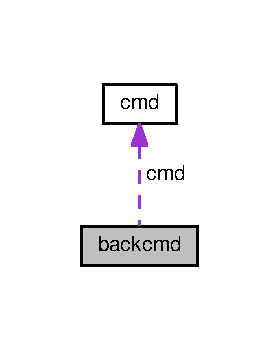
\includegraphics[width=134pt]{structbackcmd__coll__graph}
\end{center}
\end{figure}
\subsection*{Data Fields}
\begin{DoxyCompactItemize}
\item 
int \hyperlink{structbackcmd_ac765329451135abec74c45e1897abf26}{type}
\item 
struct \hyperlink{structcmd}{cmd} $\ast$ \hyperlink{structbackcmd_ae827072868c061a3985f9032a4522673}{cmd}
\end{DoxyCompactItemize}


\subsection{Detailed Description}


Definition at line 47 of file sh.\-c.



\subsection{Field Documentation}
\hypertarget{structbackcmd_ae827072868c061a3985f9032a4522673}{\index{backcmd@{backcmd}!cmd@{cmd}}
\index{cmd@{cmd}!backcmd@{backcmd}}
\subsubsection[{cmd}]{\setlength{\rightskip}{0pt plus 5cm}struct {\bf cmd}$\ast$ {\bf cmd}}}\label{structbackcmd_ae827072868c061a3985f9032a4522673}


Definition at line 49 of file sh.\-c.

\hypertarget{structbackcmd_ac765329451135abec74c45e1897abf26}{\index{backcmd@{backcmd}!type@{type}}
\index{type@{type}!backcmd@{backcmd}}
\subsubsection[{type}]{\setlength{\rightskip}{0pt plus 5cm}int type}}\label{structbackcmd_ac765329451135abec74c45e1897abf26}


Definition at line 48 of file sh.\-c.



The documentation for this struct was generated from the following file\-:\begin{DoxyCompactItemize}
\item 
user/\hyperlink{sh_8c}{sh.\-c}\end{DoxyCompactItemize}

\hypertarget{structbuf}{\section{buf Struct Reference}
\label{structbuf}\index{buf@{buf}}
}


{\ttfamily \#include $<$buf.\-h$>$}



Collaboration diagram for buf\-:
\nopagebreak
\begin{figure}[H]
\begin{center}
\leavevmode
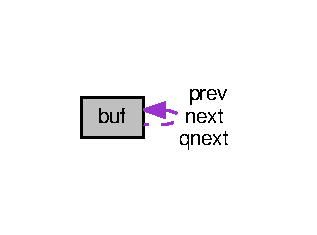
\includegraphics[width=152pt]{structbuf__coll__graph}
\end{center}
\end{figure}
\subsection*{Data Fields}
\begin{DoxyCompactItemize}
\item 
int \hyperlink{structbuf_ac8bf36fe0577cba66bccda3a6f7e80a4}{flags}
\item 
\hyperlink{types_8h_a91ad9478d81a7aaf2593e8d9c3d06a14}{uint} \hyperlink{structbuf_aaf61a1db4c34c23857104abc633d8ee6}{dev}
\item 
\hyperlink{types_8h_a91ad9478d81a7aaf2593e8d9c3d06a14}{uint} \hyperlink{structbuf_ac4ea84582da27724e7735325dd490a92}{sector}
\item 
struct \hyperlink{structbuf}{buf} $\ast$ \hyperlink{structbuf_a48c008b4a22859e25eb05af3b5c22d45}{prev}
\item 
struct \hyperlink{structbuf}{buf} $\ast$ \hyperlink{structbuf_a5a609449f1b0b08ae96fe8b29e866fd7}{next}
\item 
struct \hyperlink{structbuf}{buf} $\ast$ \hyperlink{structbuf_a479532a4750e78d1ad819ef4121f6def}{qnext}
\item 
\hyperlink{types_8h_a65f85814a8290f9797005d3b28e7e5fc}{uchar} \hyperlink{structbuf_aa6cf955e5b0bdedd2b7d1461838a1134}{data} \mbox{[}512\mbox{]}
\end{DoxyCompactItemize}


\subsection{Detailed Description}


Definition at line 4 of file buf.\-h.



\subsection{Field Documentation}
\hypertarget{structbuf_aa6cf955e5b0bdedd2b7d1461838a1134}{\index{buf@{buf}!data@{data}}
\index{data@{data}!buf@{buf}}
\subsubsection[{data}]{\setlength{\rightskip}{0pt plus 5cm}{\bf uchar} data\mbox{[}512\mbox{]}}}\label{structbuf_aa6cf955e5b0bdedd2b7d1461838a1134}


Definition at line 11 of file buf.\-h.

\hypertarget{structbuf_aaf61a1db4c34c23857104abc633d8ee6}{\index{buf@{buf}!dev@{dev}}
\index{dev@{dev}!buf@{buf}}
\subsubsection[{dev}]{\setlength{\rightskip}{0pt plus 5cm}{\bf uint} dev}}\label{structbuf_aaf61a1db4c34c23857104abc633d8ee6}


Definition at line 6 of file buf.\-h.

\hypertarget{structbuf_ac8bf36fe0577cba66bccda3a6f7e80a4}{\index{buf@{buf}!flags@{flags}}
\index{flags@{flags}!buf@{buf}}
\subsubsection[{flags}]{\setlength{\rightskip}{0pt plus 5cm}int flags}}\label{structbuf_ac8bf36fe0577cba66bccda3a6f7e80a4}


Definition at line 5 of file buf.\-h.

\hypertarget{structbuf_a5a609449f1b0b08ae96fe8b29e866fd7}{\index{buf@{buf}!next@{next}}
\index{next@{next}!buf@{buf}}
\subsubsection[{next}]{\setlength{\rightskip}{0pt plus 5cm}struct {\bf buf}$\ast$ next}}\label{structbuf_a5a609449f1b0b08ae96fe8b29e866fd7}


Definition at line 9 of file buf.\-h.

\hypertarget{structbuf_a48c008b4a22859e25eb05af3b5c22d45}{\index{buf@{buf}!prev@{prev}}
\index{prev@{prev}!buf@{buf}}
\subsubsection[{prev}]{\setlength{\rightskip}{0pt plus 5cm}struct {\bf buf}$\ast$ prev}}\label{structbuf_a48c008b4a22859e25eb05af3b5c22d45}


Definition at line 8 of file buf.\-h.

\hypertarget{structbuf_a479532a4750e78d1ad819ef4121f6def}{\index{buf@{buf}!qnext@{qnext}}
\index{qnext@{qnext}!buf@{buf}}
\subsubsection[{qnext}]{\setlength{\rightskip}{0pt plus 5cm}struct {\bf buf}$\ast$ qnext}}\label{structbuf_a479532a4750e78d1ad819ef4121f6def}


Definition at line 10 of file buf.\-h.

\hypertarget{structbuf_ac4ea84582da27724e7735325dd490a92}{\index{buf@{buf}!sector@{sector}}
\index{sector@{sector}!buf@{buf}}
\subsubsection[{sector}]{\setlength{\rightskip}{0pt plus 5cm}{\bf uint} sector}}\label{structbuf_ac4ea84582da27724e7735325dd490a92}


Definition at line 7 of file buf.\-h.



The documentation for this struct was generated from the following file\-:\begin{DoxyCompactItemize}
\item 
kernel/\hyperlink{buf_8h}{buf.\-h}\end{DoxyCompactItemize}

\hypertarget{structcmd}{\section{cmd Struct Reference}
\label{structcmd}\index{cmd@{cmd}}
}
\subsection*{Data Fields}
\begin{DoxyCompactItemize}
\item 
int \hyperlink{structcmd_ac765329451135abec74c45e1897abf26}{type}
\end{DoxyCompactItemize}


\subsection{Detailed Description}


Definition at line 16 of file sh.\-c.



\subsection{Field Documentation}
\hypertarget{structcmd_ac765329451135abec74c45e1897abf26}{\index{cmd@{cmd}!type@{type}}
\index{type@{type}!cmd@{cmd}}
\subsubsection[{type}]{\setlength{\rightskip}{0pt plus 5cm}int type}}\label{structcmd_ac765329451135abec74c45e1897abf26}


Definition at line 17 of file sh.\-c.



The documentation for this struct was generated from the following file\-:\begin{DoxyCompactItemize}
\item 
user/\hyperlink{sh_8c}{sh.\-c}\end{DoxyCompactItemize}

\hypertarget{structcontext}{\section{context Struct Reference}
\label{structcontext}\index{context@{context}}
}


{\ttfamily \#include $<$proc.\-h$>$}

\subsection*{Data Fields}
\begin{DoxyCompactItemize}
\item 
\hyperlink{types_8h_a91ad9478d81a7aaf2593e8d9c3d06a14}{uint} \hyperlink{structcontext_a5d017b35dd2b40671e27c7ae6c276b23}{edi}
\item 
\hyperlink{types_8h_a91ad9478d81a7aaf2593e8d9c3d06a14}{uint} \hyperlink{structcontext_ab40e0917bb6e7e462049fc4151201f0a}{esi}
\item 
\hyperlink{types_8h_a91ad9478d81a7aaf2593e8d9c3d06a14}{uint} \hyperlink{structcontext_a685d686dce7abed5d536f3304c4692b9}{ebx}
\item 
\hyperlink{types_8h_a91ad9478d81a7aaf2593e8d9c3d06a14}{uint} \hyperlink{structcontext_a8d9d61f0e845561448cf50ddf637e6b3}{ebp}
\item 
\hyperlink{types_8h_a91ad9478d81a7aaf2593e8d9c3d06a14}{uint} \hyperlink{structcontext_ae590d07d633d3642402cd0b25e053568}{eip}
\end{DoxyCompactItemize}


\subsection{Detailed Description}


Definition at line 52 of file proc.\-h.



\subsection{Field Documentation}
\hypertarget{structcontext_a8d9d61f0e845561448cf50ddf637e6b3}{\index{context@{context}!ebp@{ebp}}
\index{ebp@{ebp}!context@{context}}
\subsubsection[{ebp}]{\setlength{\rightskip}{0pt plus 5cm}{\bf uint} ebp}}\label{structcontext_a8d9d61f0e845561448cf50ddf637e6b3}


Definition at line 56 of file proc.\-h.

\hypertarget{structcontext_a685d686dce7abed5d536f3304c4692b9}{\index{context@{context}!ebx@{ebx}}
\index{ebx@{ebx}!context@{context}}
\subsubsection[{ebx}]{\setlength{\rightskip}{0pt plus 5cm}{\bf uint} ebx}}\label{structcontext_a685d686dce7abed5d536f3304c4692b9}


Definition at line 55 of file proc.\-h.

\hypertarget{structcontext_a5d017b35dd2b40671e27c7ae6c276b23}{\index{context@{context}!edi@{edi}}
\index{edi@{edi}!context@{context}}
\subsubsection[{edi}]{\setlength{\rightskip}{0pt plus 5cm}{\bf uint} edi}}\label{structcontext_a5d017b35dd2b40671e27c7ae6c276b23}


Definition at line 53 of file proc.\-h.

\hypertarget{structcontext_ae590d07d633d3642402cd0b25e053568}{\index{context@{context}!eip@{eip}}
\index{eip@{eip}!context@{context}}
\subsubsection[{eip}]{\setlength{\rightskip}{0pt plus 5cm}{\bf uint} eip}}\label{structcontext_ae590d07d633d3642402cd0b25e053568}


Definition at line 57 of file proc.\-h.

\hypertarget{structcontext_ab40e0917bb6e7e462049fc4151201f0a}{\index{context@{context}!esi@{esi}}
\index{esi@{esi}!context@{context}}
\subsubsection[{esi}]{\setlength{\rightskip}{0pt plus 5cm}{\bf uint} esi}}\label{structcontext_ab40e0917bb6e7e462049fc4151201f0a}


Definition at line 54 of file proc.\-h.



The documentation for this struct was generated from the following file\-:\begin{DoxyCompactItemize}
\item 
kernel/\hyperlink{proc_8h}{proc.\-h}\end{DoxyCompactItemize}

\hypertarget{structcpu}{\section{cpu Struct Reference}
\label{structcpu}\index{cpu@{cpu}}
}


{\ttfamily \#include $<$proc.\-h$>$}



Collaboration diagram for cpu\-:
\nopagebreak
\begin{figure}[H]
\begin{center}
\leavevmode
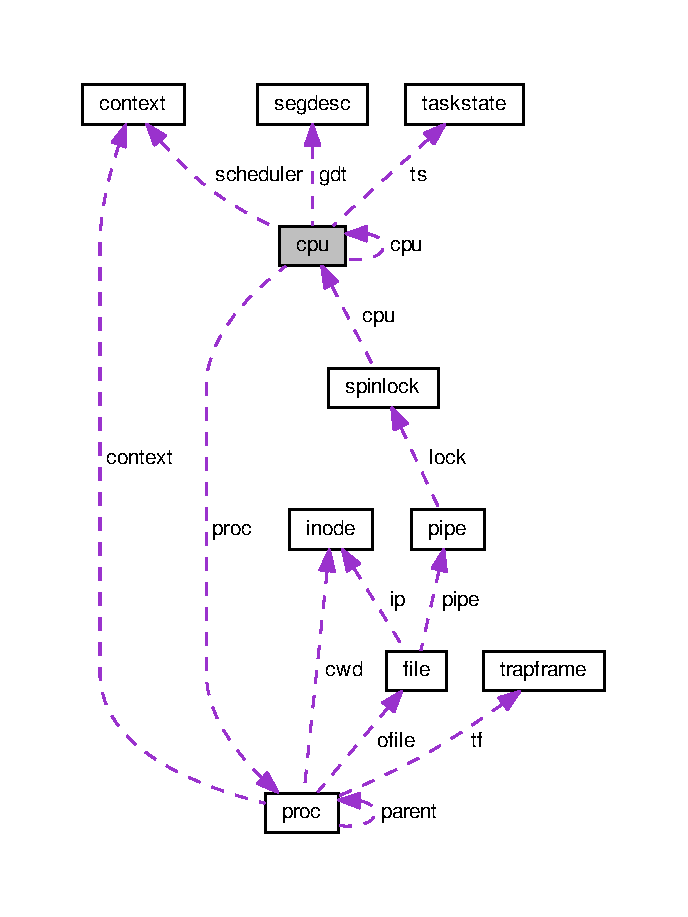
\includegraphics[width=330pt]{structcpu__coll__graph}
\end{center}
\end{figure}
\subsection*{Data Fields}
\begin{DoxyCompactItemize}
\item 
\hyperlink{types_8h_a65f85814a8290f9797005d3b28e7e5fc}{uchar} \hyperlink{structcpu_a1a656e73d1ea05b0fe2307f8a5eab1b1}{id}
\item 
struct \hyperlink{structcontext}{context} $\ast$ \hyperlink{structcpu_a98d6c9467c7b12be6c9c95a7f2cd76ee}{scheduler}
\item 
struct \hyperlink{structtaskstate}{taskstate} \hyperlink{structcpu_a20aef12941acee6e8f1a0693b1fbf681}{ts}
\item 
struct \hyperlink{structsegdesc}{segdesc} \hyperlink{structcpu_ad9d6d1fdf72705e51d5024df0f2e69a5}{gdt} \mbox{[}\hyperlink{proc_8h_a2fca412c6ed6584438e96f43ccce030a}{N\-S\-E\-G\-S}\mbox{]}
\item 
volatile \hyperlink{types_8h_a91ad9478d81a7aaf2593e8d9c3d06a14}{uint} \hyperlink{structcpu_abf27dd9e6a92da384cbfd35ec3325919}{booted}
\item 
int \hyperlink{structcpu_a47f2115921397412b52d8aa2680510ec}{ncli}
\item 
int \hyperlink{structcpu_ad4abc2486db103b06edb4f8870d1cda8}{intena}
\item 
struct \hyperlink{structcpu}{cpu} $\ast$ \hyperlink{structcpu_a01255252d6a6f1a4d5550f72dfe3a733}{cpu}
\item 
struct \hyperlink{structproc}{proc} $\ast$ \hyperlink{structcpu_a333f53825c4bbc35baa89f385e8bafc8}{proc}
\end{DoxyCompactItemize}


\subsection{Detailed Description}


Definition at line 14 of file proc.\-h.



\subsection{Field Documentation}
\hypertarget{structcpu_abf27dd9e6a92da384cbfd35ec3325919}{\index{cpu@{cpu}!booted@{booted}}
\index{booted@{booted}!cpu@{cpu}}
\subsubsection[{booted}]{\setlength{\rightskip}{0pt plus 5cm}volatile {\bf uint} booted}}\label{structcpu_abf27dd9e6a92da384cbfd35ec3325919}


Definition at line 19 of file proc.\-h.

\hypertarget{structcpu_a01255252d6a6f1a4d5550f72dfe3a733}{\index{cpu@{cpu}!cpu@{cpu}}
\index{cpu@{cpu}!cpu@{cpu}}
\subsubsection[{cpu}]{\setlength{\rightskip}{0pt plus 5cm}struct {\bf cpu}$\ast$ {\bf cpu}}}\label{structcpu_a01255252d6a6f1a4d5550f72dfe3a733}


Definition at line 24 of file proc.\-h.

\hypertarget{structcpu_ad9d6d1fdf72705e51d5024df0f2e69a5}{\index{cpu@{cpu}!gdt@{gdt}}
\index{gdt@{gdt}!cpu@{cpu}}
\subsubsection[{gdt}]{\setlength{\rightskip}{0pt plus 5cm}struct {\bf segdesc} gdt\mbox{[}{\bf N\-S\-E\-G\-S}\mbox{]}}}\label{structcpu_ad9d6d1fdf72705e51d5024df0f2e69a5}


Definition at line 18 of file proc.\-h.

\hypertarget{structcpu_a1a656e73d1ea05b0fe2307f8a5eab1b1}{\index{cpu@{cpu}!id@{id}}
\index{id@{id}!cpu@{cpu}}
\subsubsection[{id}]{\setlength{\rightskip}{0pt plus 5cm}{\bf uchar} id}}\label{structcpu_a1a656e73d1ea05b0fe2307f8a5eab1b1}


Definition at line 15 of file proc.\-h.

\hypertarget{structcpu_ad4abc2486db103b06edb4f8870d1cda8}{\index{cpu@{cpu}!intena@{intena}}
\index{intena@{intena}!cpu@{cpu}}
\subsubsection[{intena}]{\setlength{\rightskip}{0pt plus 5cm}int intena}}\label{structcpu_ad4abc2486db103b06edb4f8870d1cda8}


Definition at line 21 of file proc.\-h.

\hypertarget{structcpu_a47f2115921397412b52d8aa2680510ec}{\index{cpu@{cpu}!ncli@{ncli}}
\index{ncli@{ncli}!cpu@{cpu}}
\subsubsection[{ncli}]{\setlength{\rightskip}{0pt plus 5cm}int ncli}}\label{structcpu_a47f2115921397412b52d8aa2680510ec}


Definition at line 20 of file proc.\-h.

\hypertarget{structcpu_a333f53825c4bbc35baa89f385e8bafc8}{\index{cpu@{cpu}!proc@{proc}}
\index{proc@{proc}!cpu@{cpu}}
\subsubsection[{proc}]{\setlength{\rightskip}{0pt plus 5cm}struct {\bf proc}$\ast$ {\bf proc}}}\label{structcpu_a333f53825c4bbc35baa89f385e8bafc8}


Definition at line 25 of file proc.\-h.

\hypertarget{structcpu_a98d6c9467c7b12be6c9c95a7f2cd76ee}{\index{cpu@{cpu}!scheduler@{scheduler}}
\index{scheduler@{scheduler}!cpu@{cpu}}
\subsubsection[{scheduler}]{\setlength{\rightskip}{0pt plus 5cm}struct {\bf context}$\ast$ scheduler}}\label{structcpu_a98d6c9467c7b12be6c9c95a7f2cd76ee}


Definition at line 16 of file proc.\-h.

\hypertarget{structcpu_a20aef12941acee6e8f1a0693b1fbf681}{\index{cpu@{cpu}!ts@{ts}}
\index{ts@{ts}!cpu@{cpu}}
\subsubsection[{ts}]{\setlength{\rightskip}{0pt plus 5cm}struct {\bf taskstate} ts}}\label{structcpu_a20aef12941acee6e8f1a0693b1fbf681}


Definition at line 17 of file proc.\-h.



The documentation for this struct was generated from the following file\-:\begin{DoxyCompactItemize}
\item 
kernel/\hyperlink{proc_8h}{proc.\-h}\end{DoxyCompactItemize}

\hypertarget{structdevsw}{\section{devsw Struct Reference}
\label{structdevsw}\index{devsw@{devsw}}
}


{\ttfamily \#include $<$file.\-h$>$}

\subsection*{Data Fields}
\begin{DoxyCompactItemize}
\item 
int($\ast$ \hyperlink{structdevsw_aeeb08255a820a8e765b8065df04ba30e}{read} )(struct \hyperlink{structinode}{inode} $\ast$, char $\ast$, int)
\item 
int($\ast$ \hyperlink{structdevsw_a0239cf9da2d2be6d1d7e99446b7fc6ba}{write} )(struct \hyperlink{structinode}{inode} $\ast$, char $\ast$, int)
\end{DoxyCompactItemize}


\subsection{Detailed Description}


Definition at line 36 of file file.\-h.



\subsection{Field Documentation}
\hypertarget{structdevsw_aeeb08255a820a8e765b8065df04ba30e}{\index{devsw@{devsw}!read@{read}}
\index{read@{read}!devsw@{devsw}}
\subsubsection[{read}]{\setlength{\rightskip}{0pt plus 5cm}int($\ast$ read)(struct {\bf inode} $\ast$, char $\ast$, int)}}\label{structdevsw_aeeb08255a820a8e765b8065df04ba30e}


Definition at line 37 of file file.\-h.

\hypertarget{structdevsw_a0239cf9da2d2be6d1d7e99446b7fc6ba}{\index{devsw@{devsw}!write@{write}}
\index{write@{write}!devsw@{devsw}}
\subsubsection[{write}]{\setlength{\rightskip}{0pt plus 5cm}int($\ast$ write)(struct {\bf inode} $\ast$, char $\ast$, int)}}\label{structdevsw_a0239cf9da2d2be6d1d7e99446b7fc6ba}


Definition at line 38 of file file.\-h.



The documentation for this struct was generated from the following file\-:\begin{DoxyCompactItemize}
\item 
kernel/\hyperlink{file_8h}{file.\-h}\end{DoxyCompactItemize}

\hypertarget{structdinode}{\section{dinode Struct Reference}
\label{structdinode}\index{dinode@{dinode}}
}


{\ttfamily \#include $<$fs.\-h$>$}

\subsection*{Data Fields}
\begin{DoxyCompactItemize}
\item 
short \hyperlink{structdinode_acd579dfd50a9ea905ca697ed8707bf3b}{type}
\item 
short \hyperlink{structdinode_abe2b53edb36f3d674f052ab7254d4a3e}{major}
\item 
short \hyperlink{structdinode_adb75a8841fbdda3cb4f2373edac4f1dc}{minor}
\item 
short \hyperlink{structdinode_aa7e1ed70907ed9a2fc9c9a7c24cd0d4d}{nlink}
\item 
\hyperlink{types_8h_a91ad9478d81a7aaf2593e8d9c3d06a14}{uint} \hyperlink{structdinode_a22d26304a3b3aca97e6311f6939dd1bf}{size}
\item 
\hyperlink{types_8h_a91ad9478d81a7aaf2593e8d9c3d06a14}{uint} \hyperlink{structdinode_a94905615a8f79fd11b8f500e1bbee16d}{addrs} \mbox{[}\hyperlink{fs_8h_acd38e9532d4b3623f844b93c012a8e06}{N\-D\-I\-R\-E\-C\-T}+1\mbox{]}
\end{DoxyCompactItemize}


\subsection{Detailed Description}


Definition at line 26 of file fs.\-h.



\subsection{Field Documentation}
\hypertarget{structdinode_a94905615a8f79fd11b8f500e1bbee16d}{\index{dinode@{dinode}!addrs@{addrs}}
\index{addrs@{addrs}!dinode@{dinode}}
\subsubsection[{addrs}]{\setlength{\rightskip}{0pt plus 5cm}{\bf uint} addrs\mbox{[}{\bf N\-D\-I\-R\-E\-C\-T}+1\mbox{]}}}\label{structdinode_a94905615a8f79fd11b8f500e1bbee16d}


Definition at line 32 of file fs.\-h.

\hypertarget{structdinode_abe2b53edb36f3d674f052ab7254d4a3e}{\index{dinode@{dinode}!major@{major}}
\index{major@{major}!dinode@{dinode}}
\subsubsection[{major}]{\setlength{\rightskip}{0pt plus 5cm}short major}}\label{structdinode_abe2b53edb36f3d674f052ab7254d4a3e}


Definition at line 28 of file fs.\-h.

\hypertarget{structdinode_adb75a8841fbdda3cb4f2373edac4f1dc}{\index{dinode@{dinode}!minor@{minor}}
\index{minor@{minor}!dinode@{dinode}}
\subsubsection[{minor}]{\setlength{\rightskip}{0pt plus 5cm}short minor}}\label{structdinode_adb75a8841fbdda3cb4f2373edac4f1dc}


Definition at line 29 of file fs.\-h.

\hypertarget{structdinode_aa7e1ed70907ed9a2fc9c9a7c24cd0d4d}{\index{dinode@{dinode}!nlink@{nlink}}
\index{nlink@{nlink}!dinode@{dinode}}
\subsubsection[{nlink}]{\setlength{\rightskip}{0pt plus 5cm}short nlink}}\label{structdinode_aa7e1ed70907ed9a2fc9c9a7c24cd0d4d}


Definition at line 30 of file fs.\-h.

\hypertarget{structdinode_a22d26304a3b3aca97e6311f6939dd1bf}{\index{dinode@{dinode}!size@{size}}
\index{size@{size}!dinode@{dinode}}
\subsubsection[{size}]{\setlength{\rightskip}{0pt plus 5cm}{\bf uint} size}}\label{structdinode_a22d26304a3b3aca97e6311f6939dd1bf}


Definition at line 31 of file fs.\-h.

\hypertarget{structdinode_acd579dfd50a9ea905ca697ed8707bf3b}{\index{dinode@{dinode}!type@{type}}
\index{type@{type}!dinode@{dinode}}
\subsubsection[{type}]{\setlength{\rightskip}{0pt plus 5cm}short type}}\label{structdinode_acd579dfd50a9ea905ca697ed8707bf3b}


Definition at line 27 of file fs.\-h.



The documentation for this struct was generated from the following file\-:\begin{DoxyCompactItemize}
\item 
include/\hyperlink{fs_8h}{fs.\-h}\end{DoxyCompactItemize}

\hypertarget{structdirent}{\section{dirent Struct Reference}
\label{structdirent}\index{dirent@{dirent}}
}


{\ttfamily \#include $<$fs.\-h$>$}

\subsection*{Data Fields}
\begin{DoxyCompactItemize}
\item 
\hyperlink{types_8h_ab95f123a6c9bcfee6a343170ef8c5f69}{ushort} \hyperlink{structdirent_a2cc9c25712babfd70a85bb0dac70dcf1}{inum}
\item 
char \hyperlink{structdirent_a8ccdb14ce534c8ad0b98a76b02dcdb76}{name} \mbox{[}\hyperlink{fs_8h_a48246fb9e5cb7f6a71ebc9ebc2f06562}{D\-I\-R\-S\-I\-Z}\mbox{]}
\end{DoxyCompactItemize}


\subsection{Detailed Description}


Definition at line 50 of file fs.\-h.



\subsection{Field Documentation}
\hypertarget{structdirent_a2cc9c25712babfd70a85bb0dac70dcf1}{\index{dirent@{dirent}!inum@{inum}}
\index{inum@{inum}!dirent@{dirent}}
\subsubsection[{inum}]{\setlength{\rightskip}{0pt plus 5cm}{\bf ushort} inum}}\label{structdirent_a2cc9c25712babfd70a85bb0dac70dcf1}


Definition at line 51 of file fs.\-h.

\hypertarget{structdirent_a8ccdb14ce534c8ad0b98a76b02dcdb76}{\index{dirent@{dirent}!name@{name}}
\index{name@{name}!dirent@{dirent}}
\subsubsection[{name}]{\setlength{\rightskip}{0pt plus 5cm}char name\mbox{[}{\bf D\-I\-R\-S\-I\-Z}\mbox{]}}}\label{structdirent_a8ccdb14ce534c8ad0b98a76b02dcdb76}


Definition at line 52 of file fs.\-h.



The documentation for this struct was generated from the following file\-:\begin{DoxyCompactItemize}
\item 
include/\hyperlink{fs_8h}{fs.\-h}\end{DoxyCompactItemize}

\hypertarget{structelfhdr}{\section{elfhdr Struct Reference}
\label{structelfhdr}\index{elfhdr@{elfhdr}}
}


{\ttfamily \#include $<$elf.\-h$>$}

\subsection*{Data Fields}
\begin{DoxyCompactItemize}
\item 
\hyperlink{types_8h_a91ad9478d81a7aaf2593e8d9c3d06a14}{uint} \hyperlink{structelfhdr_a8f1cc7c49919fce5697bfbafc073003e}{magic}
\item 
\hyperlink{types_8h_a65f85814a8290f9797005d3b28e7e5fc}{uchar} \hyperlink{structelfhdr_aeba513355af321c78221dd668b203ab4}{elf} \mbox{[}12\mbox{]}
\item 
\hyperlink{types_8h_ab95f123a6c9bcfee6a343170ef8c5f69}{ushort} \hyperlink{structelfhdr_afa7787a68eb26fb33dc369c00db629ca}{type}
\item 
\hyperlink{types_8h_ab95f123a6c9bcfee6a343170ef8c5f69}{ushort} \hyperlink{structelfhdr_a46b8328012e01f0b16e4beab95b35911}{machine}
\item 
\hyperlink{types_8h_a91ad9478d81a7aaf2593e8d9c3d06a14}{uint} \hyperlink{structelfhdr_acb7e2a1d2504d82c52a9fa9b00bea040}{version}
\item 
\hyperlink{types_8h_a91ad9478d81a7aaf2593e8d9c3d06a14}{uint} \hyperlink{structelfhdr_a7fab9dad7727f5820bcce43d7649c872}{entry}
\item 
\hyperlink{types_8h_a91ad9478d81a7aaf2593e8d9c3d06a14}{uint} \hyperlink{structelfhdr_a3b2362e6eca2ec9d08ec047a8bcc13e4}{phoff}
\item 
\hyperlink{types_8h_a91ad9478d81a7aaf2593e8d9c3d06a14}{uint} \hyperlink{structelfhdr_a1f92826759f4567afd19bfe924be7f2b}{shoff}
\item 
\hyperlink{types_8h_a91ad9478d81a7aaf2593e8d9c3d06a14}{uint} \hyperlink{structelfhdr_a660f9db871d26052904976a8bfe8432d}{flags}
\item 
\hyperlink{types_8h_ab95f123a6c9bcfee6a343170ef8c5f69}{ushort} \hyperlink{structelfhdr_a671e08b578c02e1ab047c50ccb3abf84}{ehsize}
\item 
\hyperlink{types_8h_ab95f123a6c9bcfee6a343170ef8c5f69}{ushort} \hyperlink{structelfhdr_a2c1e074fc943b8556ed9b73af4dca3b3}{phentsize}
\item 
\hyperlink{types_8h_ab95f123a6c9bcfee6a343170ef8c5f69}{ushort} \hyperlink{structelfhdr_ab01d40cd4ae38ce7b110d34cc0310a6b}{phnum}
\item 
\hyperlink{types_8h_ab95f123a6c9bcfee6a343170ef8c5f69}{ushort} \hyperlink{structelfhdr_af9b275643c2083bb195d46bd28e5160f}{shentsize}
\item 
\hyperlink{types_8h_ab95f123a6c9bcfee6a343170ef8c5f69}{ushort} \hyperlink{structelfhdr_a56c0f0300ab098f73d32e42ad4d7c31e}{shnum}
\item 
\hyperlink{types_8h_ab95f123a6c9bcfee6a343170ef8c5f69}{ushort} \hyperlink{structelfhdr_a8cab050781091046b4cd1369c5988d48}{shstrndx}
\end{DoxyCompactItemize}


\subsection{Detailed Description}


Definition at line 8 of file elf.\-h.



\subsection{Field Documentation}
\hypertarget{structelfhdr_a671e08b578c02e1ab047c50ccb3abf84}{\index{elfhdr@{elfhdr}!ehsize@{ehsize}}
\index{ehsize@{ehsize}!elfhdr@{elfhdr}}
\subsubsection[{ehsize}]{\setlength{\rightskip}{0pt plus 5cm}{\bf ushort} ehsize}}\label{structelfhdr_a671e08b578c02e1ab047c50ccb3abf84}


Definition at line 18 of file elf.\-h.

\hypertarget{structelfhdr_aeba513355af321c78221dd668b203ab4}{\index{elfhdr@{elfhdr}!elf@{elf}}
\index{elf@{elf}!elfhdr@{elfhdr}}
\subsubsection[{elf}]{\setlength{\rightskip}{0pt plus 5cm}{\bf uchar} elf\mbox{[}12\mbox{]}}}\label{structelfhdr_aeba513355af321c78221dd668b203ab4}


Definition at line 10 of file elf.\-h.

\hypertarget{structelfhdr_a7fab9dad7727f5820bcce43d7649c872}{\index{elfhdr@{elfhdr}!entry@{entry}}
\index{entry@{entry}!elfhdr@{elfhdr}}
\subsubsection[{entry}]{\setlength{\rightskip}{0pt plus 5cm}{\bf uint} entry}}\label{structelfhdr_a7fab9dad7727f5820bcce43d7649c872}


Definition at line 14 of file elf.\-h.

\hypertarget{structelfhdr_a660f9db871d26052904976a8bfe8432d}{\index{elfhdr@{elfhdr}!flags@{flags}}
\index{flags@{flags}!elfhdr@{elfhdr}}
\subsubsection[{flags}]{\setlength{\rightskip}{0pt plus 5cm}{\bf uint} flags}}\label{structelfhdr_a660f9db871d26052904976a8bfe8432d}


Definition at line 17 of file elf.\-h.

\hypertarget{structelfhdr_a46b8328012e01f0b16e4beab95b35911}{\index{elfhdr@{elfhdr}!machine@{machine}}
\index{machine@{machine}!elfhdr@{elfhdr}}
\subsubsection[{machine}]{\setlength{\rightskip}{0pt plus 5cm}{\bf ushort} machine}}\label{structelfhdr_a46b8328012e01f0b16e4beab95b35911}


Definition at line 12 of file elf.\-h.

\hypertarget{structelfhdr_a8f1cc7c49919fce5697bfbafc073003e}{\index{elfhdr@{elfhdr}!magic@{magic}}
\index{magic@{magic}!elfhdr@{elfhdr}}
\subsubsection[{magic}]{\setlength{\rightskip}{0pt plus 5cm}{\bf uint} magic}}\label{structelfhdr_a8f1cc7c49919fce5697bfbafc073003e}


Definition at line 9 of file elf.\-h.

\hypertarget{structelfhdr_a2c1e074fc943b8556ed9b73af4dca3b3}{\index{elfhdr@{elfhdr}!phentsize@{phentsize}}
\index{phentsize@{phentsize}!elfhdr@{elfhdr}}
\subsubsection[{phentsize}]{\setlength{\rightskip}{0pt plus 5cm}{\bf ushort} phentsize}}\label{structelfhdr_a2c1e074fc943b8556ed9b73af4dca3b3}


Definition at line 19 of file elf.\-h.

\hypertarget{structelfhdr_ab01d40cd4ae38ce7b110d34cc0310a6b}{\index{elfhdr@{elfhdr}!phnum@{phnum}}
\index{phnum@{phnum}!elfhdr@{elfhdr}}
\subsubsection[{phnum}]{\setlength{\rightskip}{0pt plus 5cm}{\bf ushort} phnum}}\label{structelfhdr_ab01d40cd4ae38ce7b110d34cc0310a6b}


Definition at line 20 of file elf.\-h.

\hypertarget{structelfhdr_a3b2362e6eca2ec9d08ec047a8bcc13e4}{\index{elfhdr@{elfhdr}!phoff@{phoff}}
\index{phoff@{phoff}!elfhdr@{elfhdr}}
\subsubsection[{phoff}]{\setlength{\rightskip}{0pt plus 5cm}{\bf uint} phoff}}\label{structelfhdr_a3b2362e6eca2ec9d08ec047a8bcc13e4}


Definition at line 15 of file elf.\-h.

\hypertarget{structelfhdr_af9b275643c2083bb195d46bd28e5160f}{\index{elfhdr@{elfhdr}!shentsize@{shentsize}}
\index{shentsize@{shentsize}!elfhdr@{elfhdr}}
\subsubsection[{shentsize}]{\setlength{\rightskip}{0pt plus 5cm}{\bf ushort} shentsize}}\label{structelfhdr_af9b275643c2083bb195d46bd28e5160f}


Definition at line 21 of file elf.\-h.

\hypertarget{structelfhdr_a56c0f0300ab098f73d32e42ad4d7c31e}{\index{elfhdr@{elfhdr}!shnum@{shnum}}
\index{shnum@{shnum}!elfhdr@{elfhdr}}
\subsubsection[{shnum}]{\setlength{\rightskip}{0pt plus 5cm}{\bf ushort} shnum}}\label{structelfhdr_a56c0f0300ab098f73d32e42ad4d7c31e}


Definition at line 22 of file elf.\-h.

\hypertarget{structelfhdr_a1f92826759f4567afd19bfe924be7f2b}{\index{elfhdr@{elfhdr}!shoff@{shoff}}
\index{shoff@{shoff}!elfhdr@{elfhdr}}
\subsubsection[{shoff}]{\setlength{\rightskip}{0pt plus 5cm}{\bf uint} shoff}}\label{structelfhdr_a1f92826759f4567afd19bfe924be7f2b}


Definition at line 16 of file elf.\-h.

\hypertarget{structelfhdr_a8cab050781091046b4cd1369c5988d48}{\index{elfhdr@{elfhdr}!shstrndx@{shstrndx}}
\index{shstrndx@{shstrndx}!elfhdr@{elfhdr}}
\subsubsection[{shstrndx}]{\setlength{\rightskip}{0pt plus 5cm}{\bf ushort} shstrndx}}\label{structelfhdr_a8cab050781091046b4cd1369c5988d48}


Definition at line 23 of file elf.\-h.

\hypertarget{structelfhdr_afa7787a68eb26fb33dc369c00db629ca}{\index{elfhdr@{elfhdr}!type@{type}}
\index{type@{type}!elfhdr@{elfhdr}}
\subsubsection[{type}]{\setlength{\rightskip}{0pt plus 5cm}{\bf ushort} type}}\label{structelfhdr_afa7787a68eb26fb33dc369c00db629ca}


Definition at line 11 of file elf.\-h.

\hypertarget{structelfhdr_acb7e2a1d2504d82c52a9fa9b00bea040}{\index{elfhdr@{elfhdr}!version@{version}}
\index{version@{version}!elfhdr@{elfhdr}}
\subsubsection[{version}]{\setlength{\rightskip}{0pt plus 5cm}{\bf uint} version}}\label{structelfhdr_acb7e2a1d2504d82c52a9fa9b00bea040}


Definition at line 13 of file elf.\-h.



The documentation for this struct was generated from the following file\-:\begin{DoxyCompactItemize}
\item 
kernel/\hyperlink{elf_8h}{elf.\-h}\end{DoxyCompactItemize}

\hypertarget{structexeccmd}{\section{execcmd Struct Reference}
\label{structexeccmd}\index{execcmd@{execcmd}}
}
\subsection*{Data Fields}
\begin{DoxyCompactItemize}
\item 
int \hyperlink{structexeccmd_ac765329451135abec74c45e1897abf26}{type}
\item 
char $\ast$ \hyperlink{structexeccmd_aa5d608d354aee96f33c2fdca9a819305}{argv} \mbox{[}\hyperlink{sh_8c_a41101847771d39a4f0a7f9395061c629}{M\-A\-X\-A\-R\-G\-S}\mbox{]}
\item 
char $\ast$ \hyperlink{structexeccmd_aba17a3c518eb2ffd68f0219cc8c1792b}{eargv} \mbox{[}\hyperlink{sh_8c_a41101847771d39a4f0a7f9395061c629}{M\-A\-X\-A\-R\-G\-S}\mbox{]}
\end{DoxyCompactItemize}


\subsection{Detailed Description}


Definition at line 20 of file sh.\-c.



\subsection{Field Documentation}
\hypertarget{structexeccmd_aa5d608d354aee96f33c2fdca9a819305}{\index{execcmd@{execcmd}!argv@{argv}}
\index{argv@{argv}!execcmd@{execcmd}}
\subsubsection[{argv}]{\setlength{\rightskip}{0pt plus 5cm}char$\ast$ argv\mbox{[}{\bf M\-A\-X\-A\-R\-G\-S}\mbox{]}}}\label{structexeccmd_aa5d608d354aee96f33c2fdca9a819305}


Definition at line 22 of file sh.\-c.

\hypertarget{structexeccmd_aba17a3c518eb2ffd68f0219cc8c1792b}{\index{execcmd@{execcmd}!eargv@{eargv}}
\index{eargv@{eargv}!execcmd@{execcmd}}
\subsubsection[{eargv}]{\setlength{\rightskip}{0pt plus 5cm}char$\ast$ eargv\mbox{[}{\bf M\-A\-X\-A\-R\-G\-S}\mbox{]}}}\label{structexeccmd_aba17a3c518eb2ffd68f0219cc8c1792b}


Definition at line 23 of file sh.\-c.

\hypertarget{structexeccmd_ac765329451135abec74c45e1897abf26}{\index{execcmd@{execcmd}!type@{type}}
\index{type@{type}!execcmd@{execcmd}}
\subsubsection[{type}]{\setlength{\rightskip}{0pt plus 5cm}int type}}\label{structexeccmd_ac765329451135abec74c45e1897abf26}


Definition at line 21 of file sh.\-c.



The documentation for this struct was generated from the following file\-:\begin{DoxyCompactItemize}
\item 
user/\hyperlink{sh_8c}{sh.\-c}\end{DoxyCompactItemize}

\hypertarget{structfile}{\section{file Struct Reference}
\label{structfile}\index{file@{file}}
}


{\ttfamily \#include $<$file.\-h$>$}



Collaboration diagram for file\-:
\nopagebreak
\begin{figure}[H]
\begin{center}
\leavevmode
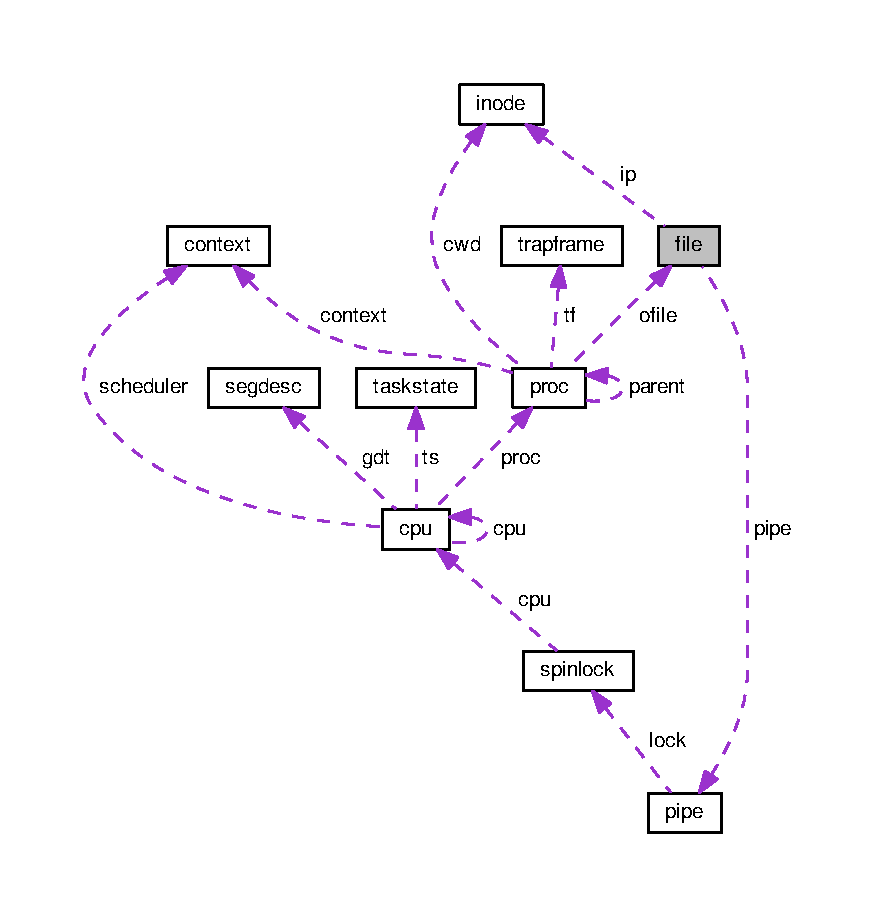
\includegraphics[width=350pt]{structfile__coll__graph}
\end{center}
\end{figure}
\subsection*{Public Types}
\begin{DoxyCompactItemize}
\item 
enum \{ \hyperlink{structfile_adc29c2ff13d900c2f185ee95427fb06ca949fd72b27639c27329b150ec9de33cd}{F\-D\-\_\-\-N\-O\-N\-E}, 
\hyperlink{structfile_adc29c2ff13d900c2f185ee95427fb06caab625bb8391962abb9337db42d7909d6}{F\-D\-\_\-\-P\-I\-P\-E}, 
\hyperlink{structfile_adc29c2ff13d900c2f185ee95427fb06ca45efb38f6972a89c2237550ef6cd542c}{F\-D\-\_\-\-I\-N\-O\-D\-E}
 \}
\end{DoxyCompactItemize}
\subsection*{Data Fields}
\begin{DoxyCompactItemize}
\item 
enum file\-:: \{ ... \}  \hyperlink{structfile_a2872497b673824bb97dd279fe716ce20}{type}
\item 
int \hyperlink{structfile_adb528a1cb1ca190150183394d082590d}{ref}
\item 
char \hyperlink{structfile_a5b131cc3952f1b648059bd61e2f49d99}{readable}
\item 
char \hyperlink{structfile_a46baf97119b7f82a588f0f603451da62}{writable}
\item 
struct \hyperlink{structpipe}{pipe} $\ast$ \hyperlink{structfile_a1e1b96aa86c12eab7047388c6538c051}{pipe}
\item 
struct \hyperlink{structinode}{inode} $\ast$ \hyperlink{structfile_a3ab9ee7e2cad8f73ff4bf973ad8d7713}{ip}
\item 
\hyperlink{types_8h_a91ad9478d81a7aaf2593e8d9c3d06a14}{uint} \hyperlink{structfile_a1aeb2e4b0cfd549f8fb46fb7e08f7e3e}{off}
\end{DoxyCompactItemize}


\subsection{Detailed Description}


Definition at line 3 of file file.\-h.



\subsection{Member Enumeration Documentation}
\hypertarget{structfile_adc29c2ff13d900c2f185ee95427fb06c}{\subsubsection[{anonymous enum}]{\setlength{\rightskip}{0pt plus 5cm}anonymous enum}}\label{structfile_adc29c2ff13d900c2f185ee95427fb06c}
\begin{Desc}
\item[Enumerator]\par
\begin{description}
\index{F\-D\-\_\-\-N\-O\-N\-E@{F\-D\-\_\-\-N\-O\-N\-E}!file@{file}}\index{file@{file}!F\-D\-\_\-\-N\-O\-N\-E@{F\-D\-\_\-\-N\-O\-N\-E}}\item[{\em 
\hypertarget{structfile_adc29c2ff13d900c2f185ee95427fb06ca949fd72b27639c27329b150ec9de33cd}{F\-D\-\_\-\-N\-O\-N\-E}\label{structfile_adc29c2ff13d900c2f185ee95427fb06ca949fd72b27639c27329b150ec9de33cd}
}]\index{F\-D\-\_\-\-P\-I\-P\-E@{F\-D\-\_\-\-P\-I\-P\-E}!file@{file}}\index{file@{file}!F\-D\-\_\-\-P\-I\-P\-E@{F\-D\-\_\-\-P\-I\-P\-E}}\item[{\em 
\hypertarget{structfile_adc29c2ff13d900c2f185ee95427fb06caab625bb8391962abb9337db42d7909d6}{F\-D\-\_\-\-P\-I\-P\-E}\label{structfile_adc29c2ff13d900c2f185ee95427fb06caab625bb8391962abb9337db42d7909d6}
}]\index{F\-D\-\_\-\-I\-N\-O\-D\-E@{F\-D\-\_\-\-I\-N\-O\-D\-E}!file@{file}}\index{file@{file}!F\-D\-\_\-\-I\-N\-O\-D\-E@{F\-D\-\_\-\-I\-N\-O\-D\-E}}\item[{\em 
\hypertarget{structfile_adc29c2ff13d900c2f185ee95427fb06ca45efb38f6972a89c2237550ef6cd542c}{F\-D\-\_\-\-I\-N\-O\-D\-E}\label{structfile_adc29c2ff13d900c2f185ee95427fb06ca45efb38f6972a89c2237550ef6cd542c}
}]\end{description}
\end{Desc}


Definition at line 4 of file file.\-h.



\subsection{Field Documentation}
\hypertarget{structfile_a3ab9ee7e2cad8f73ff4bf973ad8d7713}{\index{file@{file}!ip@{ip}}
\index{ip@{ip}!file@{file}}
\subsubsection[{ip}]{\setlength{\rightskip}{0pt plus 5cm}struct {\bf inode}$\ast$ ip}}\label{structfile_a3ab9ee7e2cad8f73ff4bf973ad8d7713}


Definition at line 9 of file file.\-h.

\hypertarget{structfile_a1aeb2e4b0cfd549f8fb46fb7e08f7e3e}{\index{file@{file}!off@{off}}
\index{off@{off}!file@{file}}
\subsubsection[{off}]{\setlength{\rightskip}{0pt plus 5cm}{\bf uint} off}}\label{structfile_a1aeb2e4b0cfd549f8fb46fb7e08f7e3e}


Definition at line 10 of file file.\-h.

\hypertarget{structfile_a1e1b96aa86c12eab7047388c6538c051}{\index{file@{file}!pipe@{pipe}}
\index{pipe@{pipe}!file@{file}}
\subsubsection[{pipe}]{\setlength{\rightskip}{0pt plus 5cm}struct {\bf pipe}$\ast$ {\bf pipe}}}\label{structfile_a1e1b96aa86c12eab7047388c6538c051}


Definition at line 8 of file file.\-h.

\hypertarget{structfile_a5b131cc3952f1b648059bd61e2f49d99}{\index{file@{file}!readable@{readable}}
\index{readable@{readable}!file@{file}}
\subsubsection[{readable}]{\setlength{\rightskip}{0pt plus 5cm}char readable}}\label{structfile_a5b131cc3952f1b648059bd61e2f49d99}


Definition at line 6 of file file.\-h.

\hypertarget{structfile_adb528a1cb1ca190150183394d082590d}{\index{file@{file}!ref@{ref}}
\index{ref@{ref}!file@{file}}
\subsubsection[{ref}]{\setlength{\rightskip}{0pt plus 5cm}int ref}}\label{structfile_adb528a1cb1ca190150183394d082590d}


Definition at line 5 of file file.\-h.

\hypertarget{structfile_a2872497b673824bb97dd279fe716ce20}{\index{file@{file}!type@{type}}
\index{type@{type}!file@{file}}
\subsubsection[{type}]{\setlength{\rightskip}{0pt plus 5cm}enum \{ ... \}   type}}\label{structfile_a2872497b673824bb97dd279fe716ce20}
\hypertarget{structfile_a46baf97119b7f82a588f0f603451da62}{\index{file@{file}!writable@{writable}}
\index{writable@{writable}!file@{file}}
\subsubsection[{writable}]{\setlength{\rightskip}{0pt plus 5cm}char writable}}\label{structfile_a46baf97119b7f82a588f0f603451da62}


Definition at line 7 of file file.\-h.



The documentation for this struct was generated from the following file\-:\begin{DoxyCompactItemize}
\item 
kernel/\hyperlink{file_8h}{file.\-h}\end{DoxyCompactItemize}

\hypertarget{structgatedesc}{\section{gatedesc Struct Reference}
\label{structgatedesc}\index{gatedesc@{gatedesc}}
}


{\ttfamily \#include $<$mmu.\-h$>$}

\subsection*{Data Fields}
\begin{DoxyCompactItemize}
\item 
\hyperlink{types_8h_a91ad9478d81a7aaf2593e8d9c3d06a14}{uint} \hyperlink{structgatedesc_a0bf2673f8a3b3345556cc583c08bfcbf}{off\-\_\-15\-\_\-0}\-: 16
\item 
\hyperlink{types_8h_a91ad9478d81a7aaf2593e8d9c3d06a14}{uint} \hyperlink{structgatedesc_a21ff1dca4ee9146feae362cb81bdb73b}{cs}\-: 16
\item 
\hyperlink{types_8h_a91ad9478d81a7aaf2593e8d9c3d06a14}{uint} \hyperlink{structgatedesc_a69a56280915744f111d56afba8b9bbe5}{args}\-: 5
\item 
\hyperlink{types_8h_a91ad9478d81a7aaf2593e8d9c3d06a14}{uint} \hyperlink{structgatedesc_a3c18a496ce0a34acbeb84338e3021797}{rsv1}\-: 3
\item 
\hyperlink{types_8h_a91ad9478d81a7aaf2593e8d9c3d06a14}{uint} \hyperlink{structgatedesc_a4e4020c6e82bee6562d5bc3c1657cafe}{type}\-: 4
\item 
\hyperlink{types_8h_a91ad9478d81a7aaf2593e8d9c3d06a14}{uint} \hyperlink{structgatedesc_a35181190d39e3d895c0ab657aceabb54}{s}\-: 1
\item 
\hyperlink{types_8h_a91ad9478d81a7aaf2593e8d9c3d06a14}{uint} \hyperlink{structgatedesc_af007c16108fee6bd537fac7128283b6e}{dpl}\-: 2
\item 
\hyperlink{types_8h_a91ad9478d81a7aaf2593e8d9c3d06a14}{uint} \hyperlink{structgatedesc_afca19e8f7fcc079e05083a7012c34ccf}{p}\-: 1
\item 
\hyperlink{types_8h_a91ad9478d81a7aaf2593e8d9c3d06a14}{uint} \hyperlink{structgatedesc_acda895cddc31853ba2be2ca38f9fc106}{off\-\_\-31\-\_\-16}\-: 16
\end{DoxyCompactItemize}


\subsection{Detailed Description}


Definition at line 186 of file mmu.\-h.



\subsection{Field Documentation}
\hypertarget{structgatedesc_a69a56280915744f111d56afba8b9bbe5}{\index{gatedesc@{gatedesc}!args@{args}}
\index{args@{args}!gatedesc@{gatedesc}}
\subsubsection[{args}]{\setlength{\rightskip}{0pt plus 5cm}{\bf uint} args}}\label{structgatedesc_a69a56280915744f111d56afba8b9bbe5}


Definition at line 189 of file mmu.\-h.

\hypertarget{structgatedesc_a21ff1dca4ee9146feae362cb81bdb73b}{\index{gatedesc@{gatedesc}!cs@{cs}}
\index{cs@{cs}!gatedesc@{gatedesc}}
\subsubsection[{cs}]{\setlength{\rightskip}{0pt plus 5cm}{\bf uint} cs}}\label{structgatedesc_a21ff1dca4ee9146feae362cb81bdb73b}


Definition at line 188 of file mmu.\-h.

\hypertarget{structgatedesc_af007c16108fee6bd537fac7128283b6e}{\index{gatedesc@{gatedesc}!dpl@{dpl}}
\index{dpl@{dpl}!gatedesc@{gatedesc}}
\subsubsection[{dpl}]{\setlength{\rightskip}{0pt plus 5cm}{\bf uint} dpl}}\label{structgatedesc_af007c16108fee6bd537fac7128283b6e}


Definition at line 193 of file mmu.\-h.

\hypertarget{structgatedesc_a0bf2673f8a3b3345556cc583c08bfcbf}{\index{gatedesc@{gatedesc}!off\-\_\-15\-\_\-0@{off\-\_\-15\-\_\-0}}
\index{off\-\_\-15\-\_\-0@{off\-\_\-15\-\_\-0}!gatedesc@{gatedesc}}
\subsubsection[{off\-\_\-15\-\_\-0}]{\setlength{\rightskip}{0pt plus 5cm}{\bf uint} off\-\_\-15\-\_\-0}}\label{structgatedesc_a0bf2673f8a3b3345556cc583c08bfcbf}


Definition at line 187 of file mmu.\-h.

\hypertarget{structgatedesc_acda895cddc31853ba2be2ca38f9fc106}{\index{gatedesc@{gatedesc}!off\-\_\-31\-\_\-16@{off\-\_\-31\-\_\-16}}
\index{off\-\_\-31\-\_\-16@{off\-\_\-31\-\_\-16}!gatedesc@{gatedesc}}
\subsubsection[{off\-\_\-31\-\_\-16}]{\setlength{\rightskip}{0pt plus 5cm}{\bf uint} off\-\_\-31\-\_\-16}}\label{structgatedesc_acda895cddc31853ba2be2ca38f9fc106}


Definition at line 195 of file mmu.\-h.

\hypertarget{structgatedesc_afca19e8f7fcc079e05083a7012c34ccf}{\index{gatedesc@{gatedesc}!p@{p}}
\index{p@{p}!gatedesc@{gatedesc}}
\subsubsection[{p}]{\setlength{\rightskip}{0pt plus 5cm}{\bf uint} p}}\label{structgatedesc_afca19e8f7fcc079e05083a7012c34ccf}


Definition at line 194 of file mmu.\-h.

\hypertarget{structgatedesc_a3c18a496ce0a34acbeb84338e3021797}{\index{gatedesc@{gatedesc}!rsv1@{rsv1}}
\index{rsv1@{rsv1}!gatedesc@{gatedesc}}
\subsubsection[{rsv1}]{\setlength{\rightskip}{0pt plus 5cm}{\bf uint} rsv1}}\label{structgatedesc_a3c18a496ce0a34acbeb84338e3021797}


Definition at line 190 of file mmu.\-h.

\hypertarget{structgatedesc_a35181190d39e3d895c0ab657aceabb54}{\index{gatedesc@{gatedesc}!s@{s}}
\index{s@{s}!gatedesc@{gatedesc}}
\subsubsection[{s}]{\setlength{\rightskip}{0pt plus 5cm}{\bf uint} s}}\label{structgatedesc_a35181190d39e3d895c0ab657aceabb54}


Definition at line 192 of file mmu.\-h.

\hypertarget{structgatedesc_a4e4020c6e82bee6562d5bc3c1657cafe}{\index{gatedesc@{gatedesc}!type@{type}}
\index{type@{type}!gatedesc@{gatedesc}}
\subsubsection[{type}]{\setlength{\rightskip}{0pt plus 5cm}{\bf uint} type}}\label{structgatedesc_a4e4020c6e82bee6562d5bc3c1657cafe}


Definition at line 191 of file mmu.\-h.



The documentation for this struct was generated from the following file\-:\begin{DoxyCompactItemize}
\item 
kernel/\hyperlink{mmu_8h}{mmu.\-h}\end{DoxyCompactItemize}

\hypertarget{unionheader}{\section{header Union Reference}
\label{unionheader}\index{header@{header}}
}


Collaboration diagram for header\-:
\nopagebreak
\begin{figure}[H]
\begin{center}
\leavevmode
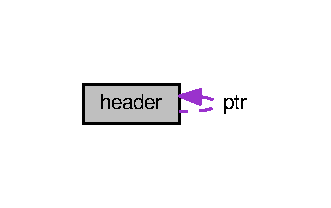
\includegraphics[width=159pt]{unionheader__coll__graph}
\end{center}
\end{figure}
\subsection*{Data Fields}
\begin{DoxyCompactItemize}
\item 
\begin{tabbing}
xx\=xx\=xx\=xx\=xx\=xx\=xx\=xx\=xx\=\kill
struct \{\\
\>union \hyperlink{unionheader}{header} $\ast$ \hyperlink{unionheader_a0e84d7fb56aa45d0a3eb7083a5ff1b63}{ptr}\\
\>\hyperlink{types_8h_a91ad9478d81a7aaf2593e8d9c3d06a14}{uint} \hyperlink{unionheader_a22d26304a3b3aca97e6311f6939dd1bf}{size}\\
\} \hyperlink{unionheader_a1e57a8830c353d3a6cd627503cb18986}{s}\\

\end{tabbing}\item 
\hyperlink{umalloc_8c_aa508dd61e627680e57643837d292d89f}{Align} \hyperlink{unionheader_a5f369a9edd645986a45d0c159773c740}{x}
\end{DoxyCompactItemize}


\subsection{Detailed Description}


Definition at line 11 of file umalloc.\-c.



\subsection{Field Documentation}
\hypertarget{unionheader_a0e84d7fb56aa45d0a3eb7083a5ff1b63}{\index{header@{header}!ptr@{ptr}}
\index{ptr@{ptr}!header@{header}}
\subsubsection[{ptr}]{\setlength{\rightskip}{0pt plus 5cm}union {\bf header}$\ast$ ptr}}\label{unionheader_a0e84d7fb56aa45d0a3eb7083a5ff1b63}


Definition at line 13 of file umalloc.\-c.

\hypertarget{unionheader_a1e57a8830c353d3a6cd627503cb18986}{\index{header@{header}!s@{s}}
\index{s@{s}!header@{header}}
\subsubsection[{s}]{\setlength{\rightskip}{0pt plus 5cm}struct \{ ... \}   s}}\label{unionheader_a1e57a8830c353d3a6cd627503cb18986}
\hypertarget{unionheader_a22d26304a3b3aca97e6311f6939dd1bf}{\index{header@{header}!size@{size}}
\index{size@{size}!header@{header}}
\subsubsection[{size}]{\setlength{\rightskip}{0pt plus 5cm}{\bf uint} size}}\label{unionheader_a22d26304a3b3aca97e6311f6939dd1bf}


Definition at line 14 of file umalloc.\-c.

\hypertarget{unionheader_a5f369a9edd645986a45d0c159773c740}{\index{header@{header}!x@{x}}
\index{x@{x}!header@{header}}
\subsubsection[{x}]{\setlength{\rightskip}{0pt plus 5cm}{\bf Align} x}}\label{unionheader_a5f369a9edd645986a45d0c159773c740}


Definition at line 16 of file umalloc.\-c.



The documentation for this union was generated from the following file\-:\begin{DoxyCompactItemize}
\item 
user/\hyperlink{umalloc_8c}{umalloc.\-c}\end{DoxyCompactItemize}

\hypertarget{structinode}{\section{inode Struct Reference}
\label{structinode}\index{inode@{inode}}
}


{\ttfamily \#include $<$file.\-h$>$}

\subsection*{Data Fields}
\begin{DoxyCompactItemize}
\item 
\hyperlink{types_8h_a91ad9478d81a7aaf2593e8d9c3d06a14}{uint} \hyperlink{structinode_aaf61a1db4c34c23857104abc633d8ee6}{dev}
\item 
\hyperlink{types_8h_a91ad9478d81a7aaf2593e8d9c3d06a14}{uint} \hyperlink{structinode_a28fdf3543c2464efb0ec94a429ef8acc}{inum}
\item 
int \hyperlink{structinode_adb528a1cb1ca190150183394d082590d}{ref}
\item 
int \hyperlink{structinode_ac8bf36fe0577cba66bccda3a6f7e80a4}{flags}
\item 
short \hyperlink{structinode_acd579dfd50a9ea905ca697ed8707bf3b}{type}
\item 
short \hyperlink{structinode_abe2b53edb36f3d674f052ab7254d4a3e}{major}
\item 
short \hyperlink{structinode_adb75a8841fbdda3cb4f2373edac4f1dc}{minor}
\item 
short \hyperlink{structinode_aa7e1ed70907ed9a2fc9c9a7c24cd0d4d}{nlink}
\item 
\hyperlink{types_8h_a91ad9478d81a7aaf2593e8d9c3d06a14}{uint} \hyperlink{structinode_a22d26304a3b3aca97e6311f6939dd1bf}{size}
\item 
\hyperlink{types_8h_a91ad9478d81a7aaf2593e8d9c3d06a14}{uint} \hyperlink{structinode_a94905615a8f79fd11b8f500e1bbee16d}{addrs} \mbox{[}\hyperlink{fs_8h_acd38e9532d4b3623f844b93c012a8e06}{N\-D\-I\-R\-E\-C\-T}+1\mbox{]}
\end{DoxyCompactItemize}


\subsection{Detailed Description}


Definition at line 16 of file file.\-h.



\subsection{Field Documentation}
\hypertarget{structinode_a94905615a8f79fd11b8f500e1bbee16d}{\index{inode@{inode}!addrs@{addrs}}
\index{addrs@{addrs}!inode@{inode}}
\subsubsection[{addrs}]{\setlength{\rightskip}{0pt plus 5cm}{\bf uint} addrs\mbox{[}{\bf N\-D\-I\-R\-E\-C\-T}+1\mbox{]}}}\label{structinode_a94905615a8f79fd11b8f500e1bbee16d}


Definition at line 27 of file file.\-h.

\hypertarget{structinode_aaf61a1db4c34c23857104abc633d8ee6}{\index{inode@{inode}!dev@{dev}}
\index{dev@{dev}!inode@{inode}}
\subsubsection[{dev}]{\setlength{\rightskip}{0pt plus 5cm}{\bf uint} dev}}\label{structinode_aaf61a1db4c34c23857104abc633d8ee6}


Definition at line 17 of file file.\-h.

\hypertarget{structinode_ac8bf36fe0577cba66bccda3a6f7e80a4}{\index{inode@{inode}!flags@{flags}}
\index{flags@{flags}!inode@{inode}}
\subsubsection[{flags}]{\setlength{\rightskip}{0pt plus 5cm}int flags}}\label{structinode_ac8bf36fe0577cba66bccda3a6f7e80a4}


Definition at line 20 of file file.\-h.

\hypertarget{structinode_a28fdf3543c2464efb0ec94a429ef8acc}{\index{inode@{inode}!inum@{inum}}
\index{inum@{inum}!inode@{inode}}
\subsubsection[{inum}]{\setlength{\rightskip}{0pt plus 5cm}{\bf uint} inum}}\label{structinode_a28fdf3543c2464efb0ec94a429ef8acc}


Definition at line 18 of file file.\-h.

\hypertarget{structinode_abe2b53edb36f3d674f052ab7254d4a3e}{\index{inode@{inode}!major@{major}}
\index{major@{major}!inode@{inode}}
\subsubsection[{major}]{\setlength{\rightskip}{0pt plus 5cm}short major}}\label{structinode_abe2b53edb36f3d674f052ab7254d4a3e}


Definition at line 23 of file file.\-h.

\hypertarget{structinode_adb75a8841fbdda3cb4f2373edac4f1dc}{\index{inode@{inode}!minor@{minor}}
\index{minor@{minor}!inode@{inode}}
\subsubsection[{minor}]{\setlength{\rightskip}{0pt plus 5cm}short minor}}\label{structinode_adb75a8841fbdda3cb4f2373edac4f1dc}


Definition at line 24 of file file.\-h.

\hypertarget{structinode_aa7e1ed70907ed9a2fc9c9a7c24cd0d4d}{\index{inode@{inode}!nlink@{nlink}}
\index{nlink@{nlink}!inode@{inode}}
\subsubsection[{nlink}]{\setlength{\rightskip}{0pt plus 5cm}short nlink}}\label{structinode_aa7e1ed70907ed9a2fc9c9a7c24cd0d4d}


Definition at line 25 of file file.\-h.

\hypertarget{structinode_adb528a1cb1ca190150183394d082590d}{\index{inode@{inode}!ref@{ref}}
\index{ref@{ref}!inode@{inode}}
\subsubsection[{ref}]{\setlength{\rightskip}{0pt plus 5cm}int ref}}\label{structinode_adb528a1cb1ca190150183394d082590d}


Definition at line 19 of file file.\-h.

\hypertarget{structinode_a22d26304a3b3aca97e6311f6939dd1bf}{\index{inode@{inode}!size@{size}}
\index{size@{size}!inode@{inode}}
\subsubsection[{size}]{\setlength{\rightskip}{0pt plus 5cm}{\bf uint} size}}\label{structinode_a22d26304a3b3aca97e6311f6939dd1bf}


Definition at line 26 of file file.\-h.

\hypertarget{structinode_acd579dfd50a9ea905ca697ed8707bf3b}{\index{inode@{inode}!type@{type}}
\index{type@{type}!inode@{inode}}
\subsubsection[{type}]{\setlength{\rightskip}{0pt plus 5cm}short type}}\label{structinode_acd579dfd50a9ea905ca697ed8707bf3b}


Definition at line 22 of file file.\-h.



The documentation for this struct was generated from the following file\-:\begin{DoxyCompactItemize}
\item 
kernel/\hyperlink{file_8h}{file.\-h}\end{DoxyCompactItemize}

\hypertarget{structioapic}{\section{ioapic Struct Reference}
\label{structioapic}\index{ioapic@{ioapic}}
}
\subsection*{Data Fields}
\begin{DoxyCompactItemize}
\item 
\hyperlink{types_8h_a91ad9478d81a7aaf2593e8d9c3d06a14}{uint} \hyperlink{structioapic_a1705e7cf67054ce9923334e3d530fcd4}{reg}
\item 
\hyperlink{types_8h_a91ad9478d81a7aaf2593e8d9c3d06a14}{uint} \hyperlink{structioapic_a099958e6ec873597215f4ef77c5cb2c3}{pad} \mbox{[}3\mbox{]}
\item 
\hyperlink{types_8h_a91ad9478d81a7aaf2593e8d9c3d06a14}{uint} \hyperlink{structioapic_a4257a9563e3f5c94350c002195cecc47}{data}
\end{DoxyCompactItemize}


\subsection{Detailed Description}


Definition at line 28 of file ioapic.\-c.



\subsection{Field Documentation}
\hypertarget{structioapic_a4257a9563e3f5c94350c002195cecc47}{\index{ioapic@{ioapic}!data@{data}}
\index{data@{data}!ioapic@{ioapic}}
\subsubsection[{data}]{\setlength{\rightskip}{0pt plus 5cm}{\bf uint} data}}\label{structioapic_a4257a9563e3f5c94350c002195cecc47}


Definition at line 31 of file ioapic.\-c.

\hypertarget{structioapic_a099958e6ec873597215f4ef77c5cb2c3}{\index{ioapic@{ioapic}!pad@{pad}}
\index{pad@{pad}!ioapic@{ioapic}}
\subsubsection[{pad}]{\setlength{\rightskip}{0pt plus 5cm}{\bf uint} pad\mbox{[}3\mbox{]}}}\label{structioapic_a099958e6ec873597215f4ef77c5cb2c3}


Definition at line 30 of file ioapic.\-c.

\hypertarget{structioapic_a1705e7cf67054ce9923334e3d530fcd4}{\index{ioapic@{ioapic}!reg@{reg}}
\index{reg@{reg}!ioapic@{ioapic}}
\subsubsection[{reg}]{\setlength{\rightskip}{0pt plus 5cm}{\bf uint} reg}}\label{structioapic_a1705e7cf67054ce9923334e3d530fcd4}


Definition at line 29 of file ioapic.\-c.



The documentation for this struct was generated from the following file\-:\begin{DoxyCompactItemize}
\item 
kernel/\hyperlink{ioapic_8c}{ioapic.\-c}\end{DoxyCompactItemize}

\hypertarget{structlistcmd}{\section{listcmd Struct Reference}
\label{structlistcmd}\index{listcmd@{listcmd}}
}


Collaboration diagram for listcmd\-:
\nopagebreak
\begin{figure}[H]
\begin{center}
\leavevmode
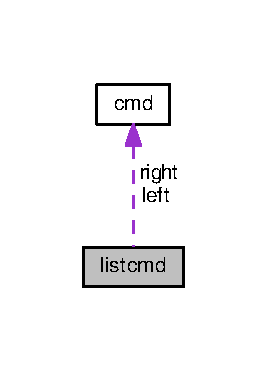
\includegraphics[width=128pt]{structlistcmd__coll__graph}
\end{center}
\end{figure}
\subsection*{Data Fields}
\begin{DoxyCompactItemize}
\item 
int \hyperlink{structlistcmd_ac765329451135abec74c45e1897abf26}{type}
\item 
struct \hyperlink{structcmd}{cmd} $\ast$ \hyperlink{structlistcmd_a69f2fa418c6e61f8b6b4e44f12a3ab4b}{left}
\item 
struct \hyperlink{structcmd}{cmd} $\ast$ \hyperlink{structlistcmd_ab5429c86b9ebd1279ea5674110a2190b}{right}
\end{DoxyCompactItemize}


\subsection{Detailed Description}


Definition at line 41 of file sh.\-c.



\subsection{Field Documentation}
\hypertarget{structlistcmd_a69f2fa418c6e61f8b6b4e44f12a3ab4b}{\index{listcmd@{listcmd}!left@{left}}
\index{left@{left}!listcmd@{listcmd}}
\subsubsection[{left}]{\setlength{\rightskip}{0pt plus 5cm}struct {\bf cmd}$\ast$ left}}\label{structlistcmd_a69f2fa418c6e61f8b6b4e44f12a3ab4b}


Definition at line 43 of file sh.\-c.

\hypertarget{structlistcmd_ab5429c86b9ebd1279ea5674110a2190b}{\index{listcmd@{listcmd}!right@{right}}
\index{right@{right}!listcmd@{listcmd}}
\subsubsection[{right}]{\setlength{\rightskip}{0pt plus 5cm}struct {\bf cmd}$\ast$ right}}\label{structlistcmd_ab5429c86b9ebd1279ea5674110a2190b}


Definition at line 44 of file sh.\-c.

\hypertarget{structlistcmd_ac765329451135abec74c45e1897abf26}{\index{listcmd@{listcmd}!type@{type}}
\index{type@{type}!listcmd@{listcmd}}
\subsubsection[{type}]{\setlength{\rightskip}{0pt plus 5cm}int type}}\label{structlistcmd_ac765329451135abec74c45e1897abf26}


Definition at line 42 of file sh.\-c.



The documentation for this struct was generated from the following file\-:\begin{DoxyCompactItemize}
\item 
user/\hyperlink{sh_8c}{sh.\-c}\end{DoxyCompactItemize}

\hypertarget{structmp}{\section{mp Struct Reference}
\label{structmp}\index{mp@{mp}}
}


{\ttfamily \#include $<$mp.\-h$>$}

\subsection*{Data Fields}
\begin{DoxyCompactItemize}
\item 
\hyperlink{types_8h_a65f85814a8290f9797005d3b28e7e5fc}{uchar} \hyperlink{structmp_a086ff3269e8b74e0f05b9120d4cac23b}{signature} \mbox{[}4\mbox{]}
\item 
void $\ast$ \hyperlink{structmp_a296f4b12bd3434a24b7f500e03c349e6}{physaddr}
\item 
\hyperlink{types_8h_a65f85814a8290f9797005d3b28e7e5fc}{uchar} \hyperlink{structmp_a180b846dc61a2dd05de3a1d6da4f3c44}{length}
\item 
\hyperlink{types_8h_a65f85814a8290f9797005d3b28e7e5fc}{uchar} \hyperlink{structmp_a3241a69299a13c78c22ccfe7ec22e90d}{specrev}
\item 
\hyperlink{types_8h_a65f85814a8290f9797005d3b28e7e5fc}{uchar} \hyperlink{structmp_a282c64bb49f098de8b45dfc535c91ac5}{checksum}
\item 
\hyperlink{types_8h_a65f85814a8290f9797005d3b28e7e5fc}{uchar} \hyperlink{structmp_a7720cfa5e476235d84bbe5bb8ad56959}{type}
\item 
\hyperlink{types_8h_a65f85814a8290f9797005d3b28e7e5fc}{uchar} \hyperlink{structmp_aaf1948d64f988c62ec336c0f5671f7ee}{imcrp}
\item 
\hyperlink{types_8h_a65f85814a8290f9797005d3b28e7e5fc}{uchar} \hyperlink{structmp_a53d99441ce014bd1cb1903e40a497d90}{reserved} \mbox{[}3\mbox{]}
\end{DoxyCompactItemize}


\subsection{Detailed Description}


Definition at line 5 of file mp.\-h.



\subsection{Field Documentation}
\hypertarget{structmp_a282c64bb49f098de8b45dfc535c91ac5}{\index{mp@{mp}!checksum@{checksum}}
\index{checksum@{checksum}!mp@{mp}}
\subsubsection[{checksum}]{\setlength{\rightskip}{0pt plus 5cm}{\bf uchar} checksum}}\label{structmp_a282c64bb49f098de8b45dfc535c91ac5}


Definition at line 10 of file mp.\-h.

\hypertarget{structmp_aaf1948d64f988c62ec336c0f5671f7ee}{\index{mp@{mp}!imcrp@{imcrp}}
\index{imcrp@{imcrp}!mp@{mp}}
\subsubsection[{imcrp}]{\setlength{\rightskip}{0pt plus 5cm}{\bf uchar} imcrp}}\label{structmp_aaf1948d64f988c62ec336c0f5671f7ee}


Definition at line 12 of file mp.\-h.

\hypertarget{structmp_a180b846dc61a2dd05de3a1d6da4f3c44}{\index{mp@{mp}!length@{length}}
\index{length@{length}!mp@{mp}}
\subsubsection[{length}]{\setlength{\rightskip}{0pt plus 5cm}{\bf uchar} length}}\label{structmp_a180b846dc61a2dd05de3a1d6da4f3c44}


Definition at line 8 of file mp.\-h.

\hypertarget{structmp_a296f4b12bd3434a24b7f500e03c349e6}{\index{mp@{mp}!physaddr@{physaddr}}
\index{physaddr@{physaddr}!mp@{mp}}
\subsubsection[{physaddr}]{\setlength{\rightskip}{0pt plus 5cm}void$\ast$ physaddr}}\label{structmp_a296f4b12bd3434a24b7f500e03c349e6}


Definition at line 7 of file mp.\-h.

\hypertarget{structmp_a53d99441ce014bd1cb1903e40a497d90}{\index{mp@{mp}!reserved@{reserved}}
\index{reserved@{reserved}!mp@{mp}}
\subsubsection[{reserved}]{\setlength{\rightskip}{0pt plus 5cm}{\bf uchar} reserved\mbox{[}3\mbox{]}}}\label{structmp_a53d99441ce014bd1cb1903e40a497d90}


Definition at line 13 of file mp.\-h.

\hypertarget{structmp_a086ff3269e8b74e0f05b9120d4cac23b}{\index{mp@{mp}!signature@{signature}}
\index{signature@{signature}!mp@{mp}}
\subsubsection[{signature}]{\setlength{\rightskip}{0pt plus 5cm}{\bf uchar} signature\mbox{[}4\mbox{]}}}\label{structmp_a086ff3269e8b74e0f05b9120d4cac23b}


Definition at line 6 of file mp.\-h.

\hypertarget{structmp_a3241a69299a13c78c22ccfe7ec22e90d}{\index{mp@{mp}!specrev@{specrev}}
\index{specrev@{specrev}!mp@{mp}}
\subsubsection[{specrev}]{\setlength{\rightskip}{0pt plus 5cm}{\bf uchar} specrev}}\label{structmp_a3241a69299a13c78c22ccfe7ec22e90d}


Definition at line 9 of file mp.\-h.

\hypertarget{structmp_a7720cfa5e476235d84bbe5bb8ad56959}{\index{mp@{mp}!type@{type}}
\index{type@{type}!mp@{mp}}
\subsubsection[{type}]{\setlength{\rightskip}{0pt plus 5cm}{\bf uchar} type}}\label{structmp_a7720cfa5e476235d84bbe5bb8ad56959}


Definition at line 11 of file mp.\-h.



The documentation for this struct was generated from the following file\-:\begin{DoxyCompactItemize}
\item 
kernel/\hyperlink{mp_8h}{mp.\-h}\end{DoxyCompactItemize}

\hypertarget{structmpconf}{\section{mpconf Struct Reference}
\label{structmpconf}\index{mpconf@{mpconf}}
}


{\ttfamily \#include $<$mp.\-h$>$}

\subsection*{Data Fields}
\begin{DoxyCompactItemize}
\item 
\hyperlink{types_8h_a65f85814a8290f9797005d3b28e7e5fc}{uchar} \hyperlink{structmpconf_a086ff3269e8b74e0f05b9120d4cac23b}{signature} \mbox{[}4\mbox{]}
\item 
\hyperlink{types_8h_ab95f123a6c9bcfee6a343170ef8c5f69}{ushort} \hyperlink{structmpconf_a795f4a78591a76d2ee53790ded8bff1f}{length}
\item 
\hyperlink{types_8h_a65f85814a8290f9797005d3b28e7e5fc}{uchar} \hyperlink{structmpconf_aa6ea6b1d12a723848cc34b199ddd8aef}{version}
\item 
\hyperlink{types_8h_a65f85814a8290f9797005d3b28e7e5fc}{uchar} \hyperlink{structmpconf_a282c64bb49f098de8b45dfc535c91ac5}{checksum}
\item 
\hyperlink{types_8h_a65f85814a8290f9797005d3b28e7e5fc}{uchar} \hyperlink{structmpconf_a09544b0a747e1c8a0ff64be0392f5c43}{product} \mbox{[}20\mbox{]}
\item 
\hyperlink{types_8h_a91ad9478d81a7aaf2593e8d9c3d06a14}{uint} $\ast$ \hyperlink{structmpconf_a4a32c8dcc1dc530dd624029c57e7cc5c}{oemtable}
\item 
\hyperlink{types_8h_ab95f123a6c9bcfee6a343170ef8c5f69}{ushort} \hyperlink{structmpconf_a1ceb9c0f37d610f220e21ff80705be9c}{oemlength}
\item 
\hyperlink{types_8h_ab95f123a6c9bcfee6a343170ef8c5f69}{ushort} \hyperlink{structmpconf_a9386724f6cb6fb5065503234c8fcf67f}{entry}
\item 
\hyperlink{types_8h_a91ad9478d81a7aaf2593e8d9c3d06a14}{uint} $\ast$ \hyperlink{structmpconf_a4a155d16bc3b1fec01b4ec50b2034005}{lapicaddr}
\item 
\hyperlink{types_8h_ab95f123a6c9bcfee6a343170ef8c5f69}{ushort} \hyperlink{structmpconf_a74abe1c31d3783b9bb39334ffad032b6}{xlength}
\item 
\hyperlink{types_8h_a65f85814a8290f9797005d3b28e7e5fc}{uchar} \hyperlink{structmpconf_a6f8d578004c11e0bdbf514588ccb1697}{xchecksum}
\item 
\hyperlink{types_8h_a65f85814a8290f9797005d3b28e7e5fc}{uchar} \hyperlink{structmpconf_a8d5874ade2fd6c06fdfd5530f0ec417d}{reserved}
\end{DoxyCompactItemize}


\subsection{Detailed Description}


Definition at line 16 of file mp.\-h.



\subsection{Field Documentation}
\hypertarget{structmpconf_a282c64bb49f098de8b45dfc535c91ac5}{\index{mpconf@{mpconf}!checksum@{checksum}}
\index{checksum@{checksum}!mpconf@{mpconf}}
\subsubsection[{checksum}]{\setlength{\rightskip}{0pt plus 5cm}{\bf uchar} checksum}}\label{structmpconf_a282c64bb49f098de8b45dfc535c91ac5}


Definition at line 20 of file mp.\-h.

\hypertarget{structmpconf_a9386724f6cb6fb5065503234c8fcf67f}{\index{mpconf@{mpconf}!entry@{entry}}
\index{entry@{entry}!mpconf@{mpconf}}
\subsubsection[{entry}]{\setlength{\rightskip}{0pt plus 5cm}{\bf ushort} entry}}\label{structmpconf_a9386724f6cb6fb5065503234c8fcf67f}


Definition at line 24 of file mp.\-h.

\hypertarget{structmpconf_a4a155d16bc3b1fec01b4ec50b2034005}{\index{mpconf@{mpconf}!lapicaddr@{lapicaddr}}
\index{lapicaddr@{lapicaddr}!mpconf@{mpconf}}
\subsubsection[{lapicaddr}]{\setlength{\rightskip}{0pt plus 5cm}{\bf uint}$\ast$ lapicaddr}}\label{structmpconf_a4a155d16bc3b1fec01b4ec50b2034005}


Definition at line 25 of file mp.\-h.

\hypertarget{structmpconf_a795f4a78591a76d2ee53790ded8bff1f}{\index{mpconf@{mpconf}!length@{length}}
\index{length@{length}!mpconf@{mpconf}}
\subsubsection[{length}]{\setlength{\rightskip}{0pt plus 5cm}{\bf ushort} length}}\label{structmpconf_a795f4a78591a76d2ee53790ded8bff1f}


Definition at line 18 of file mp.\-h.

\hypertarget{structmpconf_a1ceb9c0f37d610f220e21ff80705be9c}{\index{mpconf@{mpconf}!oemlength@{oemlength}}
\index{oemlength@{oemlength}!mpconf@{mpconf}}
\subsubsection[{oemlength}]{\setlength{\rightskip}{0pt plus 5cm}{\bf ushort} oemlength}}\label{structmpconf_a1ceb9c0f37d610f220e21ff80705be9c}


Definition at line 23 of file mp.\-h.

\hypertarget{structmpconf_a4a32c8dcc1dc530dd624029c57e7cc5c}{\index{mpconf@{mpconf}!oemtable@{oemtable}}
\index{oemtable@{oemtable}!mpconf@{mpconf}}
\subsubsection[{oemtable}]{\setlength{\rightskip}{0pt plus 5cm}{\bf uint}$\ast$ oemtable}}\label{structmpconf_a4a32c8dcc1dc530dd624029c57e7cc5c}


Definition at line 22 of file mp.\-h.

\hypertarget{structmpconf_a09544b0a747e1c8a0ff64be0392f5c43}{\index{mpconf@{mpconf}!product@{product}}
\index{product@{product}!mpconf@{mpconf}}
\subsubsection[{product}]{\setlength{\rightskip}{0pt plus 5cm}{\bf uchar} product\mbox{[}20\mbox{]}}}\label{structmpconf_a09544b0a747e1c8a0ff64be0392f5c43}


Definition at line 21 of file mp.\-h.

\hypertarget{structmpconf_a8d5874ade2fd6c06fdfd5530f0ec417d}{\index{mpconf@{mpconf}!reserved@{reserved}}
\index{reserved@{reserved}!mpconf@{mpconf}}
\subsubsection[{reserved}]{\setlength{\rightskip}{0pt plus 5cm}{\bf uchar} reserved}}\label{structmpconf_a8d5874ade2fd6c06fdfd5530f0ec417d}


Definition at line 28 of file mp.\-h.

\hypertarget{structmpconf_a086ff3269e8b74e0f05b9120d4cac23b}{\index{mpconf@{mpconf}!signature@{signature}}
\index{signature@{signature}!mpconf@{mpconf}}
\subsubsection[{signature}]{\setlength{\rightskip}{0pt plus 5cm}{\bf uchar} signature\mbox{[}4\mbox{]}}}\label{structmpconf_a086ff3269e8b74e0f05b9120d4cac23b}


Definition at line 17 of file mp.\-h.

\hypertarget{structmpconf_aa6ea6b1d12a723848cc34b199ddd8aef}{\index{mpconf@{mpconf}!version@{version}}
\index{version@{version}!mpconf@{mpconf}}
\subsubsection[{version}]{\setlength{\rightskip}{0pt plus 5cm}{\bf uchar} version}}\label{structmpconf_aa6ea6b1d12a723848cc34b199ddd8aef}


Definition at line 19 of file mp.\-h.

\hypertarget{structmpconf_a6f8d578004c11e0bdbf514588ccb1697}{\index{mpconf@{mpconf}!xchecksum@{xchecksum}}
\index{xchecksum@{xchecksum}!mpconf@{mpconf}}
\subsubsection[{xchecksum}]{\setlength{\rightskip}{0pt plus 5cm}{\bf uchar} xchecksum}}\label{structmpconf_a6f8d578004c11e0bdbf514588ccb1697}


Definition at line 27 of file mp.\-h.

\hypertarget{structmpconf_a74abe1c31d3783b9bb39334ffad032b6}{\index{mpconf@{mpconf}!xlength@{xlength}}
\index{xlength@{xlength}!mpconf@{mpconf}}
\subsubsection[{xlength}]{\setlength{\rightskip}{0pt plus 5cm}{\bf ushort} xlength}}\label{structmpconf_a74abe1c31d3783b9bb39334ffad032b6}


Definition at line 26 of file mp.\-h.



The documentation for this struct was generated from the following file\-:\begin{DoxyCompactItemize}
\item 
kernel/\hyperlink{mp_8h}{mp.\-h}\end{DoxyCompactItemize}

\hypertarget{structmpioapic}{\section{mpioapic Struct Reference}
\label{structmpioapic}\index{mpioapic@{mpioapic}}
}


{\ttfamily \#include $<$mp.\-h$>$}

\subsection*{Data Fields}
\begin{DoxyCompactItemize}
\item 
\hyperlink{types_8h_a65f85814a8290f9797005d3b28e7e5fc}{uchar} \hyperlink{structmpioapic_a7720cfa5e476235d84bbe5bb8ad56959}{type}
\item 
\hyperlink{types_8h_a65f85814a8290f9797005d3b28e7e5fc}{uchar} \hyperlink{structmpioapic_ad5298ed5a85376e373300bfe473b5ceb}{apicno}
\item 
\hyperlink{types_8h_a65f85814a8290f9797005d3b28e7e5fc}{uchar} \hyperlink{structmpioapic_aa6ea6b1d12a723848cc34b199ddd8aef}{version}
\item 
\hyperlink{types_8h_a65f85814a8290f9797005d3b28e7e5fc}{uchar} \hyperlink{structmpioapic_abe146a6a9523880d7ce48965f8d07b34}{flags}
\item 
\hyperlink{types_8h_a91ad9478d81a7aaf2593e8d9c3d06a14}{uint} $\ast$ \hyperlink{structmpioapic_aab4c2e8e264b16f9babb746d5e7250d5}{addr}
\end{DoxyCompactItemize}


\subsection{Detailed Description}


Definition at line 42 of file mp.\-h.



\subsection{Field Documentation}
\hypertarget{structmpioapic_aab4c2e8e264b16f9babb746d5e7250d5}{\index{mpioapic@{mpioapic}!addr@{addr}}
\index{addr@{addr}!mpioapic@{mpioapic}}
\subsubsection[{addr}]{\setlength{\rightskip}{0pt plus 5cm}{\bf uint}$\ast$ addr}}\label{structmpioapic_aab4c2e8e264b16f9babb746d5e7250d5}


Definition at line 47 of file mp.\-h.

\hypertarget{structmpioapic_ad5298ed5a85376e373300bfe473b5ceb}{\index{mpioapic@{mpioapic}!apicno@{apicno}}
\index{apicno@{apicno}!mpioapic@{mpioapic}}
\subsubsection[{apicno}]{\setlength{\rightskip}{0pt plus 5cm}{\bf uchar} apicno}}\label{structmpioapic_ad5298ed5a85376e373300bfe473b5ceb}


Definition at line 44 of file mp.\-h.

\hypertarget{structmpioapic_abe146a6a9523880d7ce48965f8d07b34}{\index{mpioapic@{mpioapic}!flags@{flags}}
\index{flags@{flags}!mpioapic@{mpioapic}}
\subsubsection[{flags}]{\setlength{\rightskip}{0pt plus 5cm}{\bf uchar} flags}}\label{structmpioapic_abe146a6a9523880d7ce48965f8d07b34}


Definition at line 46 of file mp.\-h.

\hypertarget{structmpioapic_a7720cfa5e476235d84bbe5bb8ad56959}{\index{mpioapic@{mpioapic}!type@{type}}
\index{type@{type}!mpioapic@{mpioapic}}
\subsubsection[{type}]{\setlength{\rightskip}{0pt plus 5cm}{\bf uchar} type}}\label{structmpioapic_a7720cfa5e476235d84bbe5bb8ad56959}


Definition at line 43 of file mp.\-h.

\hypertarget{structmpioapic_aa6ea6b1d12a723848cc34b199ddd8aef}{\index{mpioapic@{mpioapic}!version@{version}}
\index{version@{version}!mpioapic@{mpioapic}}
\subsubsection[{version}]{\setlength{\rightskip}{0pt plus 5cm}{\bf uchar} version}}\label{structmpioapic_aa6ea6b1d12a723848cc34b199ddd8aef}


Definition at line 45 of file mp.\-h.



The documentation for this struct was generated from the following file\-:\begin{DoxyCompactItemize}
\item 
kernel/\hyperlink{mp_8h}{mp.\-h}\end{DoxyCompactItemize}

\hypertarget{structmpproc}{\section{mpproc Struct Reference}
\label{structmpproc}\index{mpproc@{mpproc}}
}


{\ttfamily \#include $<$mp.\-h$>$}

\subsection*{Data Fields}
\begin{DoxyCompactItemize}
\item 
\hyperlink{types_8h_a65f85814a8290f9797005d3b28e7e5fc}{uchar} \hyperlink{structmpproc_a7720cfa5e476235d84bbe5bb8ad56959}{type}
\item 
\hyperlink{types_8h_a65f85814a8290f9797005d3b28e7e5fc}{uchar} \hyperlink{structmpproc_a6522b1dc7ec7c8888fb39b08b723bb9b}{apicid}
\item 
\hyperlink{types_8h_a65f85814a8290f9797005d3b28e7e5fc}{uchar} \hyperlink{structmpproc_aa6ea6b1d12a723848cc34b199ddd8aef}{version}
\item 
\hyperlink{types_8h_a65f85814a8290f9797005d3b28e7e5fc}{uchar} \hyperlink{structmpproc_abe146a6a9523880d7ce48965f8d07b34}{flags}
\item 
\hyperlink{types_8h_a65f85814a8290f9797005d3b28e7e5fc}{uchar} \hyperlink{structmpproc_a086ff3269e8b74e0f05b9120d4cac23b}{signature} \mbox{[}4\mbox{]}
\item 
\hyperlink{types_8h_a91ad9478d81a7aaf2593e8d9c3d06a14}{uint} \hyperlink{structmpproc_a2336e944364e02cfce4790bb4f0939fb}{feature}
\item 
\hyperlink{types_8h_a65f85814a8290f9797005d3b28e7e5fc}{uchar} \hyperlink{structmpproc_a5ec0760e684b75fdefef7023af0a3c72}{reserved} \mbox{[}8\mbox{]}
\end{DoxyCompactItemize}


\subsection{Detailed Description}


Definition at line 31 of file mp.\-h.



\subsection{Field Documentation}
\hypertarget{structmpproc_a6522b1dc7ec7c8888fb39b08b723bb9b}{\index{mpproc@{mpproc}!apicid@{apicid}}
\index{apicid@{apicid}!mpproc@{mpproc}}
\subsubsection[{apicid}]{\setlength{\rightskip}{0pt plus 5cm}{\bf uchar} apicid}}\label{structmpproc_a6522b1dc7ec7c8888fb39b08b723bb9b}


Definition at line 33 of file mp.\-h.

\hypertarget{structmpproc_a2336e944364e02cfce4790bb4f0939fb}{\index{mpproc@{mpproc}!feature@{feature}}
\index{feature@{feature}!mpproc@{mpproc}}
\subsubsection[{feature}]{\setlength{\rightskip}{0pt plus 5cm}{\bf uint} feature}}\label{structmpproc_a2336e944364e02cfce4790bb4f0939fb}


Definition at line 38 of file mp.\-h.

\hypertarget{structmpproc_abe146a6a9523880d7ce48965f8d07b34}{\index{mpproc@{mpproc}!flags@{flags}}
\index{flags@{flags}!mpproc@{mpproc}}
\subsubsection[{flags}]{\setlength{\rightskip}{0pt plus 5cm}{\bf uchar} flags}}\label{structmpproc_abe146a6a9523880d7ce48965f8d07b34}


Definition at line 35 of file mp.\-h.

\hypertarget{structmpproc_a5ec0760e684b75fdefef7023af0a3c72}{\index{mpproc@{mpproc}!reserved@{reserved}}
\index{reserved@{reserved}!mpproc@{mpproc}}
\subsubsection[{reserved}]{\setlength{\rightskip}{0pt plus 5cm}{\bf uchar} reserved\mbox{[}8\mbox{]}}}\label{structmpproc_a5ec0760e684b75fdefef7023af0a3c72}


Definition at line 39 of file mp.\-h.

\hypertarget{structmpproc_a086ff3269e8b74e0f05b9120d4cac23b}{\index{mpproc@{mpproc}!signature@{signature}}
\index{signature@{signature}!mpproc@{mpproc}}
\subsubsection[{signature}]{\setlength{\rightskip}{0pt plus 5cm}{\bf uchar} signature\mbox{[}4\mbox{]}}}\label{structmpproc_a086ff3269e8b74e0f05b9120d4cac23b}


Definition at line 37 of file mp.\-h.

\hypertarget{structmpproc_a7720cfa5e476235d84bbe5bb8ad56959}{\index{mpproc@{mpproc}!type@{type}}
\index{type@{type}!mpproc@{mpproc}}
\subsubsection[{type}]{\setlength{\rightskip}{0pt plus 5cm}{\bf uchar} type}}\label{structmpproc_a7720cfa5e476235d84bbe5bb8ad56959}


Definition at line 32 of file mp.\-h.

\hypertarget{structmpproc_aa6ea6b1d12a723848cc34b199ddd8aef}{\index{mpproc@{mpproc}!version@{version}}
\index{version@{version}!mpproc@{mpproc}}
\subsubsection[{version}]{\setlength{\rightskip}{0pt plus 5cm}{\bf uchar} version}}\label{structmpproc_aa6ea6b1d12a723848cc34b199ddd8aef}


Definition at line 34 of file mp.\-h.



The documentation for this struct was generated from the following file\-:\begin{DoxyCompactItemize}
\item 
kernel/\hyperlink{mp_8h}{mp.\-h}\end{DoxyCompactItemize}

\hypertarget{structpipe}{\section{pipe Struct Reference}
\label{structpipe}\index{pipe@{pipe}}
}


Collaboration diagram for pipe\-:
\nopagebreak
\begin{figure}[H]
\begin{center}
\leavevmode
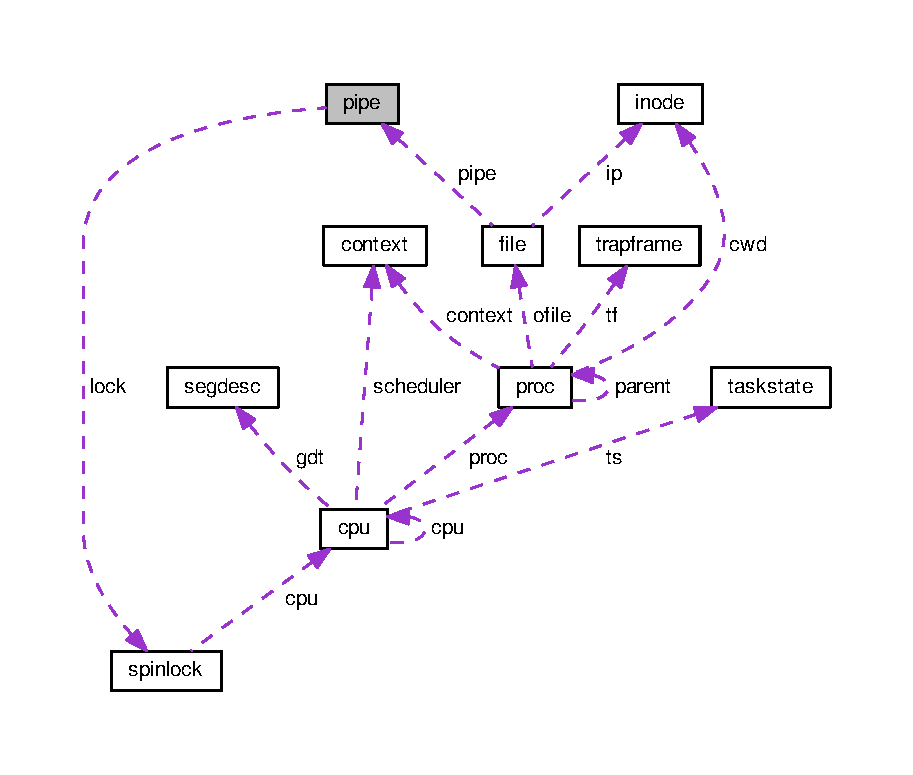
\includegraphics[width=350pt]{structpipe__coll__graph}
\end{center}
\end{figure}
\subsection*{Data Fields}
\begin{DoxyCompactItemize}
\item 
struct \hyperlink{structspinlock}{spinlock} \hyperlink{structpipe_ab28e82cd5dda7d960095706a3ea20572}{lock}
\item 
char \hyperlink{structpipe_a4b9a650598bf6f6eff13ff36793ec4f4}{data} \mbox{[}\hyperlink{pipe_8c_ad3dc9214a710d7a6c516cbaa2a12a1de}{P\-I\-P\-E\-S\-I\-Z\-E}\mbox{]}
\item 
\hyperlink{types_8h_a91ad9478d81a7aaf2593e8d9c3d06a14}{uint} \hyperlink{structpipe_a0e346df9e608d0a7d2c8538f50ec39a7}{nread}
\item 
\hyperlink{types_8h_a91ad9478d81a7aaf2593e8d9c3d06a14}{uint} \hyperlink{structpipe_a089f1ec4d2ea845105344cd1121dd3ae}{nwrite}
\item 
int \hyperlink{structpipe_a2c616f92018c3e3ed5337568ec96173f}{readopen}
\item 
int \hyperlink{structpipe_ae4254bf1d401e056beef1e2630c334e5}{writeopen}
\end{DoxyCompactItemize}


\subsection{Detailed Description}


Definition at line 12 of file pipe.\-c.



\subsection{Field Documentation}
\hypertarget{structpipe_a4b9a650598bf6f6eff13ff36793ec4f4}{\index{pipe@{pipe}!data@{data}}
\index{data@{data}!pipe@{pipe}}
\subsubsection[{data}]{\setlength{\rightskip}{0pt plus 5cm}char data\mbox{[}{\bf P\-I\-P\-E\-S\-I\-Z\-E}\mbox{]}}}\label{structpipe_a4b9a650598bf6f6eff13ff36793ec4f4}


Definition at line 14 of file pipe.\-c.

\hypertarget{structpipe_ab28e82cd5dda7d960095706a3ea20572}{\index{pipe@{pipe}!lock@{lock}}
\index{lock@{lock}!pipe@{pipe}}
\subsubsection[{lock}]{\setlength{\rightskip}{0pt plus 5cm}struct {\bf spinlock} lock}}\label{structpipe_ab28e82cd5dda7d960095706a3ea20572}


Definition at line 13 of file pipe.\-c.

\hypertarget{structpipe_a0e346df9e608d0a7d2c8538f50ec39a7}{\index{pipe@{pipe}!nread@{nread}}
\index{nread@{nread}!pipe@{pipe}}
\subsubsection[{nread}]{\setlength{\rightskip}{0pt plus 5cm}{\bf uint} nread}}\label{structpipe_a0e346df9e608d0a7d2c8538f50ec39a7}


Definition at line 15 of file pipe.\-c.

\hypertarget{structpipe_a089f1ec4d2ea845105344cd1121dd3ae}{\index{pipe@{pipe}!nwrite@{nwrite}}
\index{nwrite@{nwrite}!pipe@{pipe}}
\subsubsection[{nwrite}]{\setlength{\rightskip}{0pt plus 5cm}{\bf uint} nwrite}}\label{structpipe_a089f1ec4d2ea845105344cd1121dd3ae}


Definition at line 16 of file pipe.\-c.

\hypertarget{structpipe_a2c616f92018c3e3ed5337568ec96173f}{\index{pipe@{pipe}!readopen@{readopen}}
\index{readopen@{readopen}!pipe@{pipe}}
\subsubsection[{readopen}]{\setlength{\rightskip}{0pt plus 5cm}int readopen}}\label{structpipe_a2c616f92018c3e3ed5337568ec96173f}


Definition at line 17 of file pipe.\-c.

\hypertarget{structpipe_ae4254bf1d401e056beef1e2630c334e5}{\index{pipe@{pipe}!writeopen@{writeopen}}
\index{writeopen@{writeopen}!pipe@{pipe}}
\subsubsection[{writeopen}]{\setlength{\rightskip}{0pt plus 5cm}int writeopen}}\label{structpipe_ae4254bf1d401e056beef1e2630c334e5}


Definition at line 18 of file pipe.\-c.



The documentation for this struct was generated from the following file\-:\begin{DoxyCompactItemize}
\item 
kernel/\hyperlink{pipe_8c}{pipe.\-c}\end{DoxyCompactItemize}

\hypertarget{structpipecmd}{\section{pipecmd Struct Reference}
\label{structpipecmd}\index{pipecmd@{pipecmd}}
}


Collaboration diagram for pipecmd\-:
\nopagebreak
\begin{figure}[H]
\begin{center}
\leavevmode
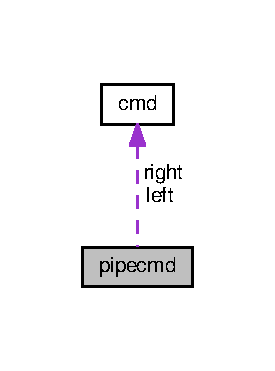
\includegraphics[width=132pt]{structpipecmd__coll__graph}
\end{center}
\end{figure}
\subsection*{Data Fields}
\begin{DoxyCompactItemize}
\item 
int \hyperlink{structpipecmd_ac765329451135abec74c45e1897abf26}{type}
\item 
struct \hyperlink{structcmd}{cmd} $\ast$ \hyperlink{structpipecmd_a69f2fa418c6e61f8b6b4e44f12a3ab4b}{left}
\item 
struct \hyperlink{structcmd}{cmd} $\ast$ \hyperlink{structpipecmd_ab5429c86b9ebd1279ea5674110a2190b}{right}
\end{DoxyCompactItemize}


\subsection{Detailed Description}


Definition at line 35 of file sh.\-c.



\subsection{Field Documentation}
\hypertarget{structpipecmd_a69f2fa418c6e61f8b6b4e44f12a3ab4b}{\index{pipecmd@{pipecmd}!left@{left}}
\index{left@{left}!pipecmd@{pipecmd}}
\subsubsection[{left}]{\setlength{\rightskip}{0pt plus 5cm}struct {\bf cmd}$\ast$ left}}\label{structpipecmd_a69f2fa418c6e61f8b6b4e44f12a3ab4b}


Definition at line 37 of file sh.\-c.

\hypertarget{structpipecmd_ab5429c86b9ebd1279ea5674110a2190b}{\index{pipecmd@{pipecmd}!right@{right}}
\index{right@{right}!pipecmd@{pipecmd}}
\subsubsection[{right}]{\setlength{\rightskip}{0pt plus 5cm}struct {\bf cmd}$\ast$ right}}\label{structpipecmd_ab5429c86b9ebd1279ea5674110a2190b}


Definition at line 38 of file sh.\-c.

\hypertarget{structpipecmd_ac765329451135abec74c45e1897abf26}{\index{pipecmd@{pipecmd}!type@{type}}
\index{type@{type}!pipecmd@{pipecmd}}
\subsubsection[{type}]{\setlength{\rightskip}{0pt plus 5cm}int type}}\label{structpipecmd_ac765329451135abec74c45e1897abf26}


Definition at line 36 of file sh.\-c.



The documentation for this struct was generated from the following file\-:\begin{DoxyCompactItemize}
\item 
user/\hyperlink{sh_8c}{sh.\-c}\end{DoxyCompactItemize}

\hypertarget{structproc}{\section{proc Struct Reference}
\label{structproc}\index{proc@{proc}}
}


{\ttfamily \#include $<$proc.\-h$>$}



Collaboration diagram for proc\-:
\nopagebreak
\begin{figure}[H]
\begin{center}
\leavevmode
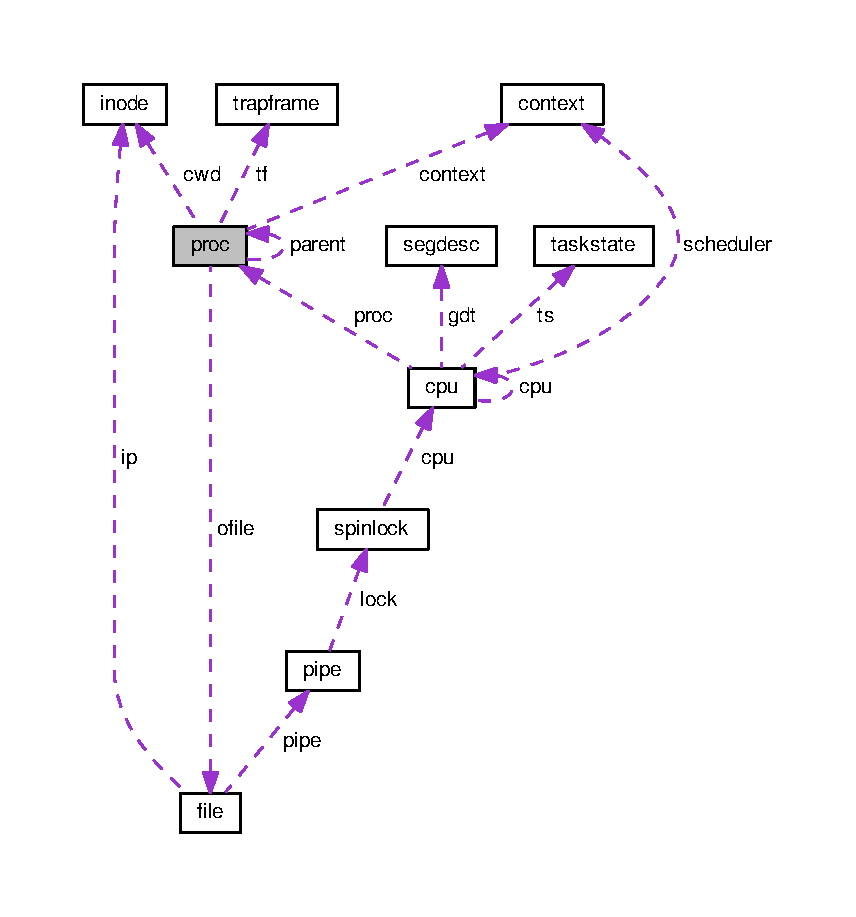
\includegraphics[width=350pt]{structproc__coll__graph}
\end{center}
\end{figure}
\subsection*{Data Fields}
\begin{DoxyCompactItemize}
\item 
\hyperlink{types_8h_a91ad9478d81a7aaf2593e8d9c3d06a14}{uint} \hyperlink{structproc_aad1b9173bbedb8de751a61a0864dcb3b}{sz}
\item 
\hyperlink{types_8h_ac131849542282b2c95dfeaf1f26dc010}{pde\-\_\-t} $\ast$ \hyperlink{structproc_abff3d102541220b0e98884d1fe2a6379}{pgdir}
\item 
char $\ast$ \hyperlink{structproc_ac9e6d1f1429b69e5e860320d95a3c5aa}{kstack}
\item 
enum \hyperlink{proc_8h_aa1ced7d2b60040fded3fa873d0c03ba7}{procstate} \hyperlink{structproc_a59425505202fc7e53a519d95707cb26b}{state}
\item 
volatile int \hyperlink{structproc_a7b6cb9255530f2807765ad74872ebdc5}{pid}
\item 
struct \hyperlink{structproc}{proc} $\ast$ \hyperlink{structproc_ad3a4594e539894e96ae2f8fea321fef2}{parent}
\item 
struct \hyperlink{structtrapframe}{trapframe} $\ast$ \hyperlink{structproc_a5a8b7d6a32569e70bff92059bd93e602}{tf}
\item 
struct \hyperlink{structcontext}{context} $\ast$ \hyperlink{structproc_a30183e0aad45d3a56e1a22d3a8fecb17}{context}
\item 
void $\ast$ \hyperlink{structproc_ae26528bc7e93e1eb8573a30309dc1424}{chan}
\item 
int \hyperlink{structproc_ab41bdc92598ccb9a0a7c2f177aa3bd5d}{killed}
\item 
struct \hyperlink{structfile}{file} $\ast$ \hyperlink{structproc_a86c51eb2e4daa425944e034bfad64fb8}{ofile} \mbox{[}\hyperlink{param_8h_a80bacbaea8dd6aecf216d85d981bcb21}{N\-O\-F\-I\-L\-E}\mbox{]}
\item 
struct \hyperlink{structinode}{inode} $\ast$ \hyperlink{structproc_a9dfc3cbb1d3bc4f1b196c07092aa64ec}{cwd}
\item 
char \hyperlink{structproc_acd328517a6cf718155c2e6e22b671ca9}{name} \mbox{[}16\mbox{]}
\end{DoxyCompactItemize}


\subsection{Detailed Description}


Definition at line 63 of file proc.\-h.



\subsection{Field Documentation}
\hypertarget{structproc_ae26528bc7e93e1eb8573a30309dc1424}{\index{proc@{proc}!chan@{chan}}
\index{chan@{chan}!proc@{proc}}
\subsubsection[{chan}]{\setlength{\rightskip}{0pt plus 5cm}void$\ast$ chan}}\label{structproc_ae26528bc7e93e1eb8573a30309dc1424}


Definition at line 72 of file proc.\-h.

\hypertarget{structproc_a30183e0aad45d3a56e1a22d3a8fecb17}{\index{proc@{proc}!context@{context}}
\index{context@{context}!proc@{proc}}
\subsubsection[{context}]{\setlength{\rightskip}{0pt plus 5cm}struct {\bf context}$\ast$ {\bf context}}}\label{structproc_a30183e0aad45d3a56e1a22d3a8fecb17}


Definition at line 71 of file proc.\-h.

\hypertarget{structproc_a9dfc3cbb1d3bc4f1b196c07092aa64ec}{\index{proc@{proc}!cwd@{cwd}}
\index{cwd@{cwd}!proc@{proc}}
\subsubsection[{cwd}]{\setlength{\rightskip}{0pt plus 5cm}struct {\bf inode}$\ast$ cwd}}\label{structproc_a9dfc3cbb1d3bc4f1b196c07092aa64ec}


Definition at line 75 of file proc.\-h.

\hypertarget{structproc_ab41bdc92598ccb9a0a7c2f177aa3bd5d}{\index{proc@{proc}!killed@{killed}}
\index{killed@{killed}!proc@{proc}}
\subsubsection[{killed}]{\setlength{\rightskip}{0pt plus 5cm}int killed}}\label{structproc_ab41bdc92598ccb9a0a7c2f177aa3bd5d}


Definition at line 73 of file proc.\-h.

\hypertarget{structproc_ac9e6d1f1429b69e5e860320d95a3c5aa}{\index{proc@{proc}!kstack@{kstack}}
\index{kstack@{kstack}!proc@{proc}}
\subsubsection[{kstack}]{\setlength{\rightskip}{0pt plus 5cm}char$\ast$ kstack}}\label{structproc_ac9e6d1f1429b69e5e860320d95a3c5aa}


Definition at line 66 of file proc.\-h.

\hypertarget{structproc_acd328517a6cf718155c2e6e22b671ca9}{\index{proc@{proc}!name@{name}}
\index{name@{name}!proc@{proc}}
\subsubsection[{name}]{\setlength{\rightskip}{0pt plus 5cm}char name\mbox{[}16\mbox{]}}}\label{structproc_acd328517a6cf718155c2e6e22b671ca9}


Definition at line 76 of file proc.\-h.

\hypertarget{structproc_a86c51eb2e4daa425944e034bfad64fb8}{\index{proc@{proc}!ofile@{ofile}}
\index{ofile@{ofile}!proc@{proc}}
\subsubsection[{ofile}]{\setlength{\rightskip}{0pt plus 5cm}struct {\bf file}$\ast$ ofile\mbox{[}{\bf N\-O\-F\-I\-L\-E}\mbox{]}}}\label{structproc_a86c51eb2e4daa425944e034bfad64fb8}


Definition at line 74 of file proc.\-h.

\hypertarget{structproc_ad3a4594e539894e96ae2f8fea321fef2}{\index{proc@{proc}!parent@{parent}}
\index{parent@{parent}!proc@{proc}}
\subsubsection[{parent}]{\setlength{\rightskip}{0pt plus 5cm}struct {\bf proc}$\ast$ parent}}\label{structproc_ad3a4594e539894e96ae2f8fea321fef2}


Definition at line 69 of file proc.\-h.

\hypertarget{structproc_abff3d102541220b0e98884d1fe2a6379}{\index{proc@{proc}!pgdir@{pgdir}}
\index{pgdir@{pgdir}!proc@{proc}}
\subsubsection[{pgdir}]{\setlength{\rightskip}{0pt plus 5cm}{\bf pde\-\_\-t}$\ast$ pgdir}}\label{structproc_abff3d102541220b0e98884d1fe2a6379}


Definition at line 65 of file proc.\-h.

\hypertarget{structproc_a7b6cb9255530f2807765ad74872ebdc5}{\index{proc@{proc}!pid@{pid}}
\index{pid@{pid}!proc@{proc}}
\subsubsection[{pid}]{\setlength{\rightskip}{0pt plus 5cm}volatile int pid}}\label{structproc_a7b6cb9255530f2807765ad74872ebdc5}


Definition at line 68 of file proc.\-h.

\hypertarget{structproc_a59425505202fc7e53a519d95707cb26b}{\index{proc@{proc}!state@{state}}
\index{state@{state}!proc@{proc}}
\subsubsection[{state}]{\setlength{\rightskip}{0pt plus 5cm}enum {\bf procstate} state}}\label{structproc_a59425505202fc7e53a519d95707cb26b}


Definition at line 67 of file proc.\-h.

\hypertarget{structproc_aad1b9173bbedb8de751a61a0864dcb3b}{\index{proc@{proc}!sz@{sz}}
\index{sz@{sz}!proc@{proc}}
\subsubsection[{sz}]{\setlength{\rightskip}{0pt plus 5cm}{\bf uint} sz}}\label{structproc_aad1b9173bbedb8de751a61a0864dcb3b}


Definition at line 64 of file proc.\-h.

\hypertarget{structproc_a5a8b7d6a32569e70bff92059bd93e602}{\index{proc@{proc}!tf@{tf}}
\index{tf@{tf}!proc@{proc}}
\subsubsection[{tf}]{\setlength{\rightskip}{0pt plus 5cm}struct {\bf trapframe}$\ast$ tf}}\label{structproc_a5a8b7d6a32569e70bff92059bd93e602}


Definition at line 70 of file proc.\-h.



The documentation for this struct was generated from the following file\-:\begin{DoxyCompactItemize}
\item 
kernel/\hyperlink{proc_8h}{proc.\-h}\end{DoxyCompactItemize}

\hypertarget{structproghdr}{\section{proghdr Struct Reference}
\label{structproghdr}\index{proghdr@{proghdr}}
}


{\ttfamily \#include $<$elf.\-h$>$}

\subsection*{Data Fields}
\begin{DoxyCompactItemize}
\item 
\hyperlink{types_8h_a91ad9478d81a7aaf2593e8d9c3d06a14}{uint} \hyperlink{structproghdr_a4e4020c6e82bee6562d5bc3c1657cafe}{type}
\item 
\hyperlink{types_8h_a91ad9478d81a7aaf2593e8d9c3d06a14}{uint} \hyperlink{structproghdr_abb6eef28c6175ceaae40067c5761fb3c}{offset}
\item 
\hyperlink{types_8h_a91ad9478d81a7aaf2593e8d9c3d06a14}{uint} \hyperlink{structproghdr_a24266ece98365336cbbb0f5cbb092148}{va}
\item 
\hyperlink{types_8h_a91ad9478d81a7aaf2593e8d9c3d06a14}{uint} \hyperlink{structproghdr_adc03a600d1b3918826d34dfb0c4bf1ab}{pa}
\item 
\hyperlink{types_8h_a91ad9478d81a7aaf2593e8d9c3d06a14}{uint} \hyperlink{structproghdr_af68648ec9784a595235d016a78d4e443}{filesz}
\item 
\hyperlink{types_8h_a91ad9478d81a7aaf2593e8d9c3d06a14}{uint} \hyperlink{structproghdr_adda66e6aa36c4d480d9a96db0653f1c0}{memsz}
\item 
\hyperlink{types_8h_a91ad9478d81a7aaf2593e8d9c3d06a14}{uint} \hyperlink{structproghdr_a660f9db871d26052904976a8bfe8432d}{flags}
\item 
\hyperlink{types_8h_a91ad9478d81a7aaf2593e8d9c3d06a14}{uint} \hyperlink{structproghdr_a8a93f1094c7ddc65184ffb84a9059862}{align}
\end{DoxyCompactItemize}


\subsection{Detailed Description}


Definition at line 27 of file elf.\-h.



\subsection{Field Documentation}
\hypertarget{structproghdr_a8a93f1094c7ddc65184ffb84a9059862}{\index{proghdr@{proghdr}!align@{align}}
\index{align@{align}!proghdr@{proghdr}}
\subsubsection[{align}]{\setlength{\rightskip}{0pt plus 5cm}{\bf uint} align}}\label{structproghdr_a8a93f1094c7ddc65184ffb84a9059862}


Definition at line 35 of file elf.\-h.

\hypertarget{structproghdr_af68648ec9784a595235d016a78d4e443}{\index{proghdr@{proghdr}!filesz@{filesz}}
\index{filesz@{filesz}!proghdr@{proghdr}}
\subsubsection[{filesz}]{\setlength{\rightskip}{0pt plus 5cm}{\bf uint} filesz}}\label{structproghdr_af68648ec9784a595235d016a78d4e443}


Definition at line 32 of file elf.\-h.

\hypertarget{structproghdr_a660f9db871d26052904976a8bfe8432d}{\index{proghdr@{proghdr}!flags@{flags}}
\index{flags@{flags}!proghdr@{proghdr}}
\subsubsection[{flags}]{\setlength{\rightskip}{0pt plus 5cm}{\bf uint} flags}}\label{structproghdr_a660f9db871d26052904976a8bfe8432d}


Definition at line 34 of file elf.\-h.

\hypertarget{structproghdr_adda66e6aa36c4d480d9a96db0653f1c0}{\index{proghdr@{proghdr}!memsz@{memsz}}
\index{memsz@{memsz}!proghdr@{proghdr}}
\subsubsection[{memsz}]{\setlength{\rightskip}{0pt plus 5cm}{\bf uint} memsz}}\label{structproghdr_adda66e6aa36c4d480d9a96db0653f1c0}


Definition at line 33 of file elf.\-h.

\hypertarget{structproghdr_abb6eef28c6175ceaae40067c5761fb3c}{\index{proghdr@{proghdr}!offset@{offset}}
\index{offset@{offset}!proghdr@{proghdr}}
\subsubsection[{offset}]{\setlength{\rightskip}{0pt plus 5cm}{\bf uint} offset}}\label{structproghdr_abb6eef28c6175ceaae40067c5761fb3c}


Definition at line 29 of file elf.\-h.

\hypertarget{structproghdr_adc03a600d1b3918826d34dfb0c4bf1ab}{\index{proghdr@{proghdr}!pa@{pa}}
\index{pa@{pa}!proghdr@{proghdr}}
\subsubsection[{pa}]{\setlength{\rightskip}{0pt plus 5cm}{\bf uint} pa}}\label{structproghdr_adc03a600d1b3918826d34dfb0c4bf1ab}


Definition at line 31 of file elf.\-h.

\hypertarget{structproghdr_a4e4020c6e82bee6562d5bc3c1657cafe}{\index{proghdr@{proghdr}!type@{type}}
\index{type@{type}!proghdr@{proghdr}}
\subsubsection[{type}]{\setlength{\rightskip}{0pt plus 5cm}{\bf uint} type}}\label{structproghdr_a4e4020c6e82bee6562d5bc3c1657cafe}


Definition at line 28 of file elf.\-h.

\hypertarget{structproghdr_a24266ece98365336cbbb0f5cbb092148}{\index{proghdr@{proghdr}!va@{va}}
\index{va@{va}!proghdr@{proghdr}}
\subsubsection[{va}]{\setlength{\rightskip}{0pt plus 5cm}{\bf uint} va}}\label{structproghdr_a24266ece98365336cbbb0f5cbb092148}


Definition at line 30 of file elf.\-h.



The documentation for this struct was generated from the following file\-:\begin{DoxyCompactItemize}
\item 
kernel/\hyperlink{elf_8h}{elf.\-h}\end{DoxyCompactItemize}

\hypertarget{structredircmd}{\section{redircmd Struct Reference}
\label{structredircmd}\index{redircmd@{redircmd}}
}


Collaboration diagram for redircmd\-:
\nopagebreak
\begin{figure}[H]
\begin{center}
\leavevmode
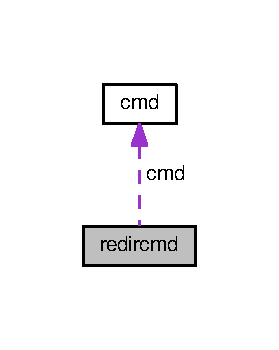
\includegraphics[width=134pt]{structredircmd__coll__graph}
\end{center}
\end{figure}
\subsection*{Data Fields}
\begin{DoxyCompactItemize}
\item 
int \hyperlink{structredircmd_ac765329451135abec74c45e1897abf26}{type}
\item 
struct \hyperlink{structcmd}{cmd} $\ast$ \hyperlink{structredircmd_ae827072868c061a3985f9032a4522673}{cmd}
\item 
char $\ast$ \hyperlink{structredircmd_adf16cd437526a5c5e0e0af87745acbb8}{file}
\item 
char $\ast$ \hyperlink{structredircmd_ab5755209db30db6cbfdec21ca15015db}{efile}
\item 
int \hyperlink{structredircmd_a1ea5d0cb93f22f7d0fdf804bd68c3326}{mode}
\item 
int \hyperlink{structredircmd_a6f8059414f0228f0256115e024eeed4b}{fd}
\end{DoxyCompactItemize}


\subsection{Detailed Description}


Definition at line 26 of file sh.\-c.



\subsection{Field Documentation}
\hypertarget{structredircmd_ae827072868c061a3985f9032a4522673}{\index{redircmd@{redircmd}!cmd@{cmd}}
\index{cmd@{cmd}!redircmd@{redircmd}}
\subsubsection[{cmd}]{\setlength{\rightskip}{0pt plus 5cm}struct {\bf cmd}$\ast$ {\bf cmd}}}\label{structredircmd_ae827072868c061a3985f9032a4522673}


Definition at line 28 of file sh.\-c.

\hypertarget{structredircmd_ab5755209db30db6cbfdec21ca15015db}{\index{redircmd@{redircmd}!efile@{efile}}
\index{efile@{efile}!redircmd@{redircmd}}
\subsubsection[{efile}]{\setlength{\rightskip}{0pt plus 5cm}char$\ast$ efile}}\label{structredircmd_ab5755209db30db6cbfdec21ca15015db}


Definition at line 30 of file sh.\-c.

\hypertarget{structredircmd_a6f8059414f0228f0256115e024eeed4b}{\index{redircmd@{redircmd}!fd@{fd}}
\index{fd@{fd}!redircmd@{redircmd}}
\subsubsection[{fd}]{\setlength{\rightskip}{0pt plus 5cm}int fd}}\label{structredircmd_a6f8059414f0228f0256115e024eeed4b}


Definition at line 32 of file sh.\-c.

\hypertarget{structredircmd_adf16cd437526a5c5e0e0af87745acbb8}{\index{redircmd@{redircmd}!file@{file}}
\index{file@{file}!redircmd@{redircmd}}
\subsubsection[{file}]{\setlength{\rightskip}{0pt plus 5cm}char$\ast$ {\bf file}}}\label{structredircmd_adf16cd437526a5c5e0e0af87745acbb8}


Definition at line 29 of file sh.\-c.

\hypertarget{structredircmd_a1ea5d0cb93f22f7d0fdf804bd68c3326}{\index{redircmd@{redircmd}!mode@{mode}}
\index{mode@{mode}!redircmd@{redircmd}}
\subsubsection[{mode}]{\setlength{\rightskip}{0pt plus 5cm}int mode}}\label{structredircmd_a1ea5d0cb93f22f7d0fdf804bd68c3326}


Definition at line 31 of file sh.\-c.

\hypertarget{structredircmd_ac765329451135abec74c45e1897abf26}{\index{redircmd@{redircmd}!type@{type}}
\index{type@{type}!redircmd@{redircmd}}
\subsubsection[{type}]{\setlength{\rightskip}{0pt plus 5cm}int type}}\label{structredircmd_ac765329451135abec74c45e1897abf26}


Definition at line 27 of file sh.\-c.



The documentation for this struct was generated from the following file\-:\begin{DoxyCompactItemize}
\item 
user/\hyperlink{sh_8c}{sh.\-c}\end{DoxyCompactItemize}

\hypertarget{structrun}{\section{run Struct Reference}
\label{structrun}\index{run@{run}}
}


Collaboration diagram for run\-:
\nopagebreak
\begin{figure}[H]
\begin{center}
\leavevmode
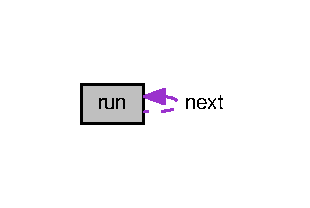
\includegraphics[width=149pt]{structrun__coll__graph}
\end{center}
\end{figure}
\subsection*{Data Fields}
\begin{DoxyCompactItemize}
\item 
struct \hyperlink{structrun}{run} $\ast$ \hyperlink{structrun_afa37bad156291ffb38122b28ebd546ef}{next}
\end{DoxyCompactItemize}


\subsection{Detailed Description}


Definition at line 11 of file kalloc.\-c.



\subsection{Field Documentation}
\hypertarget{structrun_afa37bad156291ffb38122b28ebd546ef}{\index{run@{run}!next@{next}}
\index{next@{next}!run@{run}}
\subsubsection[{next}]{\setlength{\rightskip}{0pt plus 5cm}struct {\bf run}$\ast$ next}}\label{structrun_afa37bad156291ffb38122b28ebd546ef}


Definition at line 12 of file kalloc.\-c.



The documentation for this struct was generated from the following file\-:\begin{DoxyCompactItemize}
\item 
kernel/\hyperlink{kalloc_8c}{kalloc.\-c}\end{DoxyCompactItemize}

\hypertarget{structsegdesc}{\section{segdesc Struct Reference}
\label{structsegdesc}\index{segdesc@{segdesc}}
}


{\ttfamily \#include $<$mmu.\-h$>$}

\subsection*{Data Fields}
\begin{DoxyCompactItemize}
\item 
\hyperlink{types_8h_a91ad9478d81a7aaf2593e8d9c3d06a14}{uint} \hyperlink{structsegdesc_aa05f1f5cdd8d56cc9f8c331ceeda7813}{lim\-\_\-15\-\_\-0}\-: 16
\item 
\hyperlink{types_8h_a91ad9478d81a7aaf2593e8d9c3d06a14}{uint} \hyperlink{structsegdesc_a5b20f16107a37790349fb5c3856c6c01}{base\-\_\-15\-\_\-0}\-: 16
\item 
\hyperlink{types_8h_a91ad9478d81a7aaf2593e8d9c3d06a14}{uint} \hyperlink{structsegdesc_a80d2085d2e280c3bbd1420fb452680e2}{base\-\_\-23\-\_\-16}\-: 8
\item 
\hyperlink{types_8h_a91ad9478d81a7aaf2593e8d9c3d06a14}{uint} \hyperlink{structsegdesc_a4e4020c6e82bee6562d5bc3c1657cafe}{type}\-: 4
\item 
\hyperlink{types_8h_a91ad9478d81a7aaf2593e8d9c3d06a14}{uint} \hyperlink{structsegdesc_a35181190d39e3d895c0ab657aceabb54}{s}\-: 1
\item 
\hyperlink{types_8h_a91ad9478d81a7aaf2593e8d9c3d06a14}{uint} \hyperlink{structsegdesc_af007c16108fee6bd537fac7128283b6e}{dpl}\-: 2
\item 
\hyperlink{types_8h_a91ad9478d81a7aaf2593e8d9c3d06a14}{uint} \hyperlink{structsegdesc_afca19e8f7fcc079e05083a7012c34ccf}{p}\-: 1
\item 
\hyperlink{types_8h_a91ad9478d81a7aaf2593e8d9c3d06a14}{uint} \hyperlink{structsegdesc_abe13981739b3fcc0205ee38da6c18cc9}{lim\-\_\-19\-\_\-16}\-: 4
\item 
\hyperlink{types_8h_a91ad9478d81a7aaf2593e8d9c3d06a14}{uint} \hyperlink{structsegdesc_a3fe31ffafb8c060bbfce5cc88bc4a7c3}{avl}\-: 1
\item 
\hyperlink{types_8h_a91ad9478d81a7aaf2593e8d9c3d06a14}{uint} \hyperlink{structsegdesc_a3c18a496ce0a34acbeb84338e3021797}{rsv1}\-: 1
\item 
\hyperlink{types_8h_a91ad9478d81a7aaf2593e8d9c3d06a14}{uint} \hyperlink{structsegdesc_a04ab5582b63d915355818185ba20a9c4}{db}\-: 1
\item 
\hyperlink{types_8h_a91ad9478d81a7aaf2593e8d9c3d06a14}{uint} \hyperlink{structsegdesc_a507f46d64a589eaa3bf729789889283c}{g}\-: 1
\item 
\hyperlink{types_8h_a91ad9478d81a7aaf2593e8d9c3d06a14}{uint} \hyperlink{structsegdesc_aa4e2821f8c7d1fb00ed552f59d07f59a}{base\-\_\-31\-\_\-24}\-: 8
\end{DoxyCompactItemize}


\subsection{Detailed Description}


Definition at line 43 of file mmu.\-h.



\subsection{Field Documentation}
\hypertarget{structsegdesc_a3fe31ffafb8c060bbfce5cc88bc4a7c3}{\index{segdesc@{segdesc}!avl@{avl}}
\index{avl@{avl}!segdesc@{segdesc}}
\subsubsection[{avl}]{\setlength{\rightskip}{0pt plus 5cm}{\bf uint} avl}}\label{structsegdesc_a3fe31ffafb8c060bbfce5cc88bc4a7c3}


Definition at line 52 of file mmu.\-h.

\hypertarget{structsegdesc_a5b20f16107a37790349fb5c3856c6c01}{\index{segdesc@{segdesc}!base\-\_\-15\-\_\-0@{base\-\_\-15\-\_\-0}}
\index{base\-\_\-15\-\_\-0@{base\-\_\-15\-\_\-0}!segdesc@{segdesc}}
\subsubsection[{base\-\_\-15\-\_\-0}]{\setlength{\rightskip}{0pt plus 5cm}{\bf uint} base\-\_\-15\-\_\-0}}\label{structsegdesc_a5b20f16107a37790349fb5c3856c6c01}


Definition at line 45 of file mmu.\-h.

\hypertarget{structsegdesc_a80d2085d2e280c3bbd1420fb452680e2}{\index{segdesc@{segdesc}!base\-\_\-23\-\_\-16@{base\-\_\-23\-\_\-16}}
\index{base\-\_\-23\-\_\-16@{base\-\_\-23\-\_\-16}!segdesc@{segdesc}}
\subsubsection[{base\-\_\-23\-\_\-16}]{\setlength{\rightskip}{0pt plus 5cm}{\bf uint} base\-\_\-23\-\_\-16}}\label{structsegdesc_a80d2085d2e280c3bbd1420fb452680e2}


Definition at line 46 of file mmu.\-h.

\hypertarget{structsegdesc_aa4e2821f8c7d1fb00ed552f59d07f59a}{\index{segdesc@{segdesc}!base\-\_\-31\-\_\-24@{base\-\_\-31\-\_\-24}}
\index{base\-\_\-31\-\_\-24@{base\-\_\-31\-\_\-24}!segdesc@{segdesc}}
\subsubsection[{base\-\_\-31\-\_\-24}]{\setlength{\rightskip}{0pt plus 5cm}{\bf uint} base\-\_\-31\-\_\-24}}\label{structsegdesc_aa4e2821f8c7d1fb00ed552f59d07f59a}


Definition at line 56 of file mmu.\-h.

\hypertarget{structsegdesc_a04ab5582b63d915355818185ba20a9c4}{\index{segdesc@{segdesc}!db@{db}}
\index{db@{db}!segdesc@{segdesc}}
\subsubsection[{db}]{\setlength{\rightskip}{0pt plus 5cm}{\bf uint} db}}\label{structsegdesc_a04ab5582b63d915355818185ba20a9c4}


Definition at line 54 of file mmu.\-h.

\hypertarget{structsegdesc_af007c16108fee6bd537fac7128283b6e}{\index{segdesc@{segdesc}!dpl@{dpl}}
\index{dpl@{dpl}!segdesc@{segdesc}}
\subsubsection[{dpl}]{\setlength{\rightskip}{0pt plus 5cm}{\bf uint} dpl}}\label{structsegdesc_af007c16108fee6bd537fac7128283b6e}


Definition at line 49 of file mmu.\-h.

\hypertarget{structsegdesc_a507f46d64a589eaa3bf729789889283c}{\index{segdesc@{segdesc}!g@{g}}
\index{g@{g}!segdesc@{segdesc}}
\subsubsection[{g}]{\setlength{\rightskip}{0pt plus 5cm}{\bf uint} g}}\label{structsegdesc_a507f46d64a589eaa3bf729789889283c}


Definition at line 55 of file mmu.\-h.

\hypertarget{structsegdesc_aa05f1f5cdd8d56cc9f8c331ceeda7813}{\index{segdesc@{segdesc}!lim\-\_\-15\-\_\-0@{lim\-\_\-15\-\_\-0}}
\index{lim\-\_\-15\-\_\-0@{lim\-\_\-15\-\_\-0}!segdesc@{segdesc}}
\subsubsection[{lim\-\_\-15\-\_\-0}]{\setlength{\rightskip}{0pt plus 5cm}{\bf uint} lim\-\_\-15\-\_\-0}}\label{structsegdesc_aa05f1f5cdd8d56cc9f8c331ceeda7813}


Definition at line 44 of file mmu.\-h.

\hypertarget{structsegdesc_abe13981739b3fcc0205ee38da6c18cc9}{\index{segdesc@{segdesc}!lim\-\_\-19\-\_\-16@{lim\-\_\-19\-\_\-16}}
\index{lim\-\_\-19\-\_\-16@{lim\-\_\-19\-\_\-16}!segdesc@{segdesc}}
\subsubsection[{lim\-\_\-19\-\_\-16}]{\setlength{\rightskip}{0pt plus 5cm}{\bf uint} lim\-\_\-19\-\_\-16}}\label{structsegdesc_abe13981739b3fcc0205ee38da6c18cc9}


Definition at line 51 of file mmu.\-h.

\hypertarget{structsegdesc_afca19e8f7fcc079e05083a7012c34ccf}{\index{segdesc@{segdesc}!p@{p}}
\index{p@{p}!segdesc@{segdesc}}
\subsubsection[{p}]{\setlength{\rightskip}{0pt plus 5cm}{\bf uint} p}}\label{structsegdesc_afca19e8f7fcc079e05083a7012c34ccf}


Definition at line 50 of file mmu.\-h.

\hypertarget{structsegdesc_a3c18a496ce0a34acbeb84338e3021797}{\index{segdesc@{segdesc}!rsv1@{rsv1}}
\index{rsv1@{rsv1}!segdesc@{segdesc}}
\subsubsection[{rsv1}]{\setlength{\rightskip}{0pt plus 5cm}{\bf uint} rsv1}}\label{structsegdesc_a3c18a496ce0a34acbeb84338e3021797}


Definition at line 53 of file mmu.\-h.

\hypertarget{structsegdesc_a35181190d39e3d895c0ab657aceabb54}{\index{segdesc@{segdesc}!s@{s}}
\index{s@{s}!segdesc@{segdesc}}
\subsubsection[{s}]{\setlength{\rightskip}{0pt plus 5cm}{\bf uint} s}}\label{structsegdesc_a35181190d39e3d895c0ab657aceabb54}


Definition at line 48 of file mmu.\-h.

\hypertarget{structsegdesc_a4e4020c6e82bee6562d5bc3c1657cafe}{\index{segdesc@{segdesc}!type@{type}}
\index{type@{type}!segdesc@{segdesc}}
\subsubsection[{type}]{\setlength{\rightskip}{0pt plus 5cm}{\bf uint} type}}\label{structsegdesc_a4e4020c6e82bee6562d5bc3c1657cafe}


Definition at line 47 of file mmu.\-h.



The documentation for this struct was generated from the following file\-:\begin{DoxyCompactItemize}
\item 
kernel/\hyperlink{mmu_8h}{mmu.\-h}\end{DoxyCompactItemize}

\hypertarget{structspinlock}{\section{spinlock Struct Reference}
\label{structspinlock}\index{spinlock@{spinlock}}
}


{\ttfamily \#include $<$spinlock.\-h$>$}



Collaboration diagram for spinlock\-:
\nopagebreak
\begin{figure}[H]
\begin{center}
\leavevmode
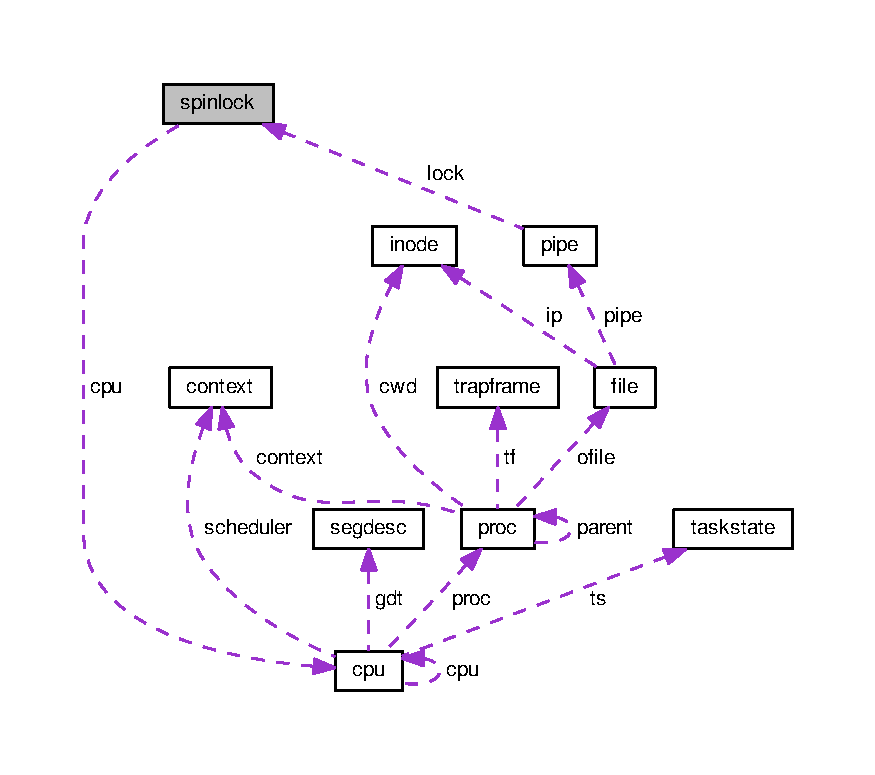
\includegraphics[width=350pt]{structspinlock__coll__graph}
\end{center}
\end{figure}
\subsection*{Data Fields}
\begin{DoxyCompactItemize}
\item 
\hyperlink{types_8h_a91ad9478d81a7aaf2593e8d9c3d06a14}{uint} \hyperlink{structspinlock_a2468e5b98a0b805a0a174eda5d09c6ad}{locked}
\item 
char $\ast$ \hyperlink{structspinlock_a5ac083a645d964373f022d03df4849c8}{name}
\item 
struct \hyperlink{structcpu}{cpu} $\ast$ \hyperlink{structspinlock_a01255252d6a6f1a4d5550f72dfe3a733}{cpu}
\item 
\hyperlink{types_8h_a91ad9478d81a7aaf2593e8d9c3d06a14}{uint} \hyperlink{structspinlock_a96a0f9277e455aac1e0f848607cb1a2d}{pcs} \mbox{[}10\mbox{]}
\end{DoxyCompactItemize}


\subsection{Detailed Description}


Definition at line 5 of file spinlock.\-h.



\subsection{Field Documentation}
\hypertarget{structspinlock_a01255252d6a6f1a4d5550f72dfe3a733}{\index{spinlock@{spinlock}!cpu@{cpu}}
\index{cpu@{cpu}!spinlock@{spinlock}}
\subsubsection[{cpu}]{\setlength{\rightskip}{0pt plus 5cm}struct {\bf cpu}$\ast$ {\bf cpu}}}\label{structspinlock_a01255252d6a6f1a4d5550f72dfe3a733}


Definition at line 10 of file spinlock.\-h.

\hypertarget{structspinlock_a2468e5b98a0b805a0a174eda5d09c6ad}{\index{spinlock@{spinlock}!locked@{locked}}
\index{locked@{locked}!spinlock@{spinlock}}
\subsubsection[{locked}]{\setlength{\rightskip}{0pt plus 5cm}{\bf uint} locked}}\label{structspinlock_a2468e5b98a0b805a0a174eda5d09c6ad}


Definition at line 6 of file spinlock.\-h.

\hypertarget{structspinlock_a5ac083a645d964373f022d03df4849c8}{\index{spinlock@{spinlock}!name@{name}}
\index{name@{name}!spinlock@{spinlock}}
\subsubsection[{name}]{\setlength{\rightskip}{0pt plus 5cm}char$\ast$ name}}\label{structspinlock_a5ac083a645d964373f022d03df4849c8}


Definition at line 9 of file spinlock.\-h.

\hypertarget{structspinlock_a96a0f9277e455aac1e0f848607cb1a2d}{\index{spinlock@{spinlock}!pcs@{pcs}}
\index{pcs@{pcs}!spinlock@{spinlock}}
\subsubsection[{pcs}]{\setlength{\rightskip}{0pt plus 5cm}{\bf uint} pcs\mbox{[}10\mbox{]}}}\label{structspinlock_a96a0f9277e455aac1e0f848607cb1a2d}


Definition at line 11 of file spinlock.\-h.



The documentation for this struct was generated from the following file\-:\begin{DoxyCompactItemize}
\item 
kernel/\hyperlink{spinlock_8h}{spinlock.\-h}\end{DoxyCompactItemize}

\hypertarget{structstat}{\section{stat Struct Reference}
\label{structstat}\index{stat@{stat}}
}


{\ttfamily \#include $<$stat.\-h$>$}

\subsection*{Data Fields}
\begin{DoxyCompactItemize}
\item 
short \hyperlink{structstat_acd579dfd50a9ea905ca697ed8707bf3b}{type}
\item 
int \hyperlink{structstat_a22c99b5ae74d0e3dcf126f0d950538e4}{dev}
\item 
\hyperlink{types_8h_a91ad9478d81a7aaf2593e8d9c3d06a14}{uint} \hyperlink{structstat_a928a75be0d96aba7e4cfeacfab8cdeb2}{ino}
\item 
short \hyperlink{structstat_aa7e1ed70907ed9a2fc9c9a7c24cd0d4d}{nlink}
\item 
\hyperlink{types_8h_a91ad9478d81a7aaf2593e8d9c3d06a14}{uint} \hyperlink{structstat_a22d26304a3b3aca97e6311f6939dd1bf}{size}
\end{DoxyCompactItemize}


\subsection{Detailed Description}


Definition at line 10 of file stat.\-h.



\subsection{Field Documentation}
\hypertarget{structstat_a22c99b5ae74d0e3dcf126f0d950538e4}{\index{stat@{stat}!dev@{dev}}
\index{dev@{dev}!stat@{stat}}
\subsubsection[{dev}]{\setlength{\rightskip}{0pt plus 5cm}int dev}}\label{structstat_a22c99b5ae74d0e3dcf126f0d950538e4}


Definition at line 12 of file stat.\-h.

\hypertarget{structstat_a928a75be0d96aba7e4cfeacfab8cdeb2}{\index{stat@{stat}!ino@{ino}}
\index{ino@{ino}!stat@{stat}}
\subsubsection[{ino}]{\setlength{\rightskip}{0pt plus 5cm}{\bf uint} ino}}\label{structstat_a928a75be0d96aba7e4cfeacfab8cdeb2}


Definition at line 13 of file stat.\-h.

\hypertarget{structstat_aa7e1ed70907ed9a2fc9c9a7c24cd0d4d}{\index{stat@{stat}!nlink@{nlink}}
\index{nlink@{nlink}!stat@{stat}}
\subsubsection[{nlink}]{\setlength{\rightskip}{0pt plus 5cm}short nlink}}\label{structstat_aa7e1ed70907ed9a2fc9c9a7c24cd0d4d}


Definition at line 14 of file stat.\-h.

\hypertarget{structstat_a22d26304a3b3aca97e6311f6939dd1bf}{\index{stat@{stat}!size@{size}}
\index{size@{size}!stat@{stat}}
\subsubsection[{size}]{\setlength{\rightskip}{0pt plus 5cm}{\bf uint} size}}\label{structstat_a22d26304a3b3aca97e6311f6939dd1bf}


Definition at line 15 of file stat.\-h.

\hypertarget{structstat_acd579dfd50a9ea905ca697ed8707bf3b}{\index{stat@{stat}!type@{type}}
\index{type@{type}!stat@{stat}}
\subsubsection[{type}]{\setlength{\rightskip}{0pt plus 5cm}short type}}\label{structstat_acd579dfd50a9ea905ca697ed8707bf3b}


Definition at line 11 of file stat.\-h.



The documentation for this struct was generated from the following file\-:\begin{DoxyCompactItemize}
\item 
include/\hyperlink{stat_8h}{stat.\-h}\end{DoxyCompactItemize}

\hypertarget{structsuperblock}{\section{superblock Struct Reference}
\label{structsuperblock}\index{superblock@{superblock}}
}


{\ttfamily \#include $<$fs.\-h$>$}

\subsection*{Data Fields}
\begin{DoxyCompactItemize}
\item 
\hyperlink{types_8h_a91ad9478d81a7aaf2593e8d9c3d06a14}{uint} \hyperlink{structsuperblock_a22d26304a3b3aca97e6311f6939dd1bf}{size}
\item 
\hyperlink{types_8h_a91ad9478d81a7aaf2593e8d9c3d06a14}{uint} \hyperlink{structsuperblock_acca6315b99c9786037236e521f8b2556}{nblocks}
\item 
\hyperlink{types_8h_a91ad9478d81a7aaf2593e8d9c3d06a14}{uint} \hyperlink{structsuperblock_a9df4c697e9b13fc3226bb66e46b3b409}{ninodes}
\end{DoxyCompactItemize}


\subsection{Detailed Description}


Definition at line 15 of file fs.\-h.



\subsection{Field Documentation}
\hypertarget{structsuperblock_acca6315b99c9786037236e521f8b2556}{\index{superblock@{superblock}!nblocks@{nblocks}}
\index{nblocks@{nblocks}!superblock@{superblock}}
\subsubsection[{nblocks}]{\setlength{\rightskip}{0pt plus 5cm}{\bf uint} nblocks}}\label{structsuperblock_acca6315b99c9786037236e521f8b2556}


Definition at line 17 of file fs.\-h.

\hypertarget{structsuperblock_a9df4c697e9b13fc3226bb66e46b3b409}{\index{superblock@{superblock}!ninodes@{ninodes}}
\index{ninodes@{ninodes}!superblock@{superblock}}
\subsubsection[{ninodes}]{\setlength{\rightskip}{0pt plus 5cm}{\bf uint} ninodes}}\label{structsuperblock_a9df4c697e9b13fc3226bb66e46b3b409}


Definition at line 18 of file fs.\-h.

\hypertarget{structsuperblock_a22d26304a3b3aca97e6311f6939dd1bf}{\index{superblock@{superblock}!size@{size}}
\index{size@{size}!superblock@{superblock}}
\subsubsection[{size}]{\setlength{\rightskip}{0pt plus 5cm}{\bf uint} size}}\label{structsuperblock_a22d26304a3b3aca97e6311f6939dd1bf}


Definition at line 16 of file fs.\-h.



The documentation for this struct was generated from the following file\-:\begin{DoxyCompactItemize}
\item 
include/\hyperlink{fs_8h}{fs.\-h}\end{DoxyCompactItemize}

\hypertarget{structtaskstate}{\section{taskstate Struct Reference}
\label{structtaskstate}\index{taskstate@{taskstate}}
}


{\ttfamily \#include $<$mmu.\-h$>$}

\subsection*{Data Fields}
\begin{DoxyCompactItemize}
\item 
\hyperlink{types_8h_a91ad9478d81a7aaf2593e8d9c3d06a14}{uint} \hyperlink{structtaskstate_ae657c87971475ad47724bbcf3e4537e6}{link}
\item 
\hyperlink{types_8h_a91ad9478d81a7aaf2593e8d9c3d06a14}{uint} \hyperlink{structtaskstate_a105b1107443842b93c88ade5254ab9d2}{esp0}
\item 
\hyperlink{types_8h_ab95f123a6c9bcfee6a343170ef8c5f69}{ushort} \hyperlink{structtaskstate_a9648f5e19cd4adcae28d51f6e326d6f4}{ss0}
\item 
\hyperlink{types_8h_ab95f123a6c9bcfee6a343170ef8c5f69}{ushort} \hyperlink{structtaskstate_af1bf63d9df475699143c50918af7c3b9}{padding1}
\item 
\hyperlink{types_8h_a91ad9478d81a7aaf2593e8d9c3d06a14}{uint} $\ast$ \hyperlink{structtaskstate_acd0d21f790060be5f36be94fed86be0f}{esp1}
\item 
\hyperlink{types_8h_ab95f123a6c9bcfee6a343170ef8c5f69}{ushort} \hyperlink{structtaskstate_afc8f1257b84a23a426b3b5b2794d98df}{ss1}
\item 
\hyperlink{types_8h_ab95f123a6c9bcfee6a343170ef8c5f69}{ushort} \hyperlink{structtaskstate_a352099edda0c7698cf5f352878346448}{padding2}
\item 
\hyperlink{types_8h_a91ad9478d81a7aaf2593e8d9c3d06a14}{uint} $\ast$ \hyperlink{structtaskstate_abfc181b97d3a3bf5afdc662d5d345764}{esp2}
\item 
\hyperlink{types_8h_ab95f123a6c9bcfee6a343170ef8c5f69}{ushort} \hyperlink{structtaskstate_a6a7c092edd3dde61711a7e349e4eb191}{ss2}
\item 
\hyperlink{types_8h_ab95f123a6c9bcfee6a343170ef8c5f69}{ushort} \hyperlink{structtaskstate_a1d1a645b86f97ca1844887d6178675aa}{padding3}
\item 
void $\ast$ \hyperlink{structtaskstate_a915afcdc183379971c3d7f5d665017c6}{cr3}
\item 
\hyperlink{types_8h_a91ad9478d81a7aaf2593e8d9c3d06a14}{uint} $\ast$ \hyperlink{structtaskstate_a20cd904809a7d6c9d5e573f1539e8436}{eip}
\item 
\hyperlink{types_8h_a91ad9478d81a7aaf2593e8d9c3d06a14}{uint} \hyperlink{structtaskstate_a96d2765012333ea2615dda6ac2521d61}{eflags}
\item 
\hyperlink{types_8h_a91ad9478d81a7aaf2593e8d9c3d06a14}{uint} \hyperlink{structtaskstate_a6f7100b52071edc47e593b1c6a9453cb}{eax}
\item 
\hyperlink{types_8h_a91ad9478d81a7aaf2593e8d9c3d06a14}{uint} \hyperlink{structtaskstate_ab36b3e14ca8cf65ad02ef0b466bff207}{ecx}
\item 
\hyperlink{types_8h_a91ad9478d81a7aaf2593e8d9c3d06a14}{uint} \hyperlink{structtaskstate_a897b994c12c5e0174809a975642fe7fb}{edx}
\item 
\hyperlink{types_8h_a91ad9478d81a7aaf2593e8d9c3d06a14}{uint} \hyperlink{structtaskstate_a685d686dce7abed5d536f3304c4692b9}{ebx}
\item 
\hyperlink{types_8h_a91ad9478d81a7aaf2593e8d9c3d06a14}{uint} $\ast$ \hyperlink{structtaskstate_aff753e3f000b68547dbcfb705b97983d}{esp}
\item 
\hyperlink{types_8h_a91ad9478d81a7aaf2593e8d9c3d06a14}{uint} $\ast$ \hyperlink{structtaskstate_a5f72bae04632ef90f7c23e2ea4702c43}{ebp}
\item 
\hyperlink{types_8h_a91ad9478d81a7aaf2593e8d9c3d06a14}{uint} \hyperlink{structtaskstate_ab40e0917bb6e7e462049fc4151201f0a}{esi}
\item 
\hyperlink{types_8h_a91ad9478d81a7aaf2593e8d9c3d06a14}{uint} \hyperlink{structtaskstate_a5d017b35dd2b40671e27c7ae6c276b23}{edi}
\item 
\hyperlink{types_8h_ab95f123a6c9bcfee6a343170ef8c5f69}{ushort} \hyperlink{structtaskstate_a926406c155a1238da40552b902622ab2}{es}
\item 
\hyperlink{types_8h_ab95f123a6c9bcfee6a343170ef8c5f69}{ushort} \hyperlink{structtaskstate_a2b559818ffd02a68e4d5ac320237a025}{padding4}
\item 
\hyperlink{types_8h_ab95f123a6c9bcfee6a343170ef8c5f69}{ushort} \hyperlink{structtaskstate_a2c1a506f83f7be334e4128748f4a2eaa}{cs}
\item 
\hyperlink{types_8h_ab95f123a6c9bcfee6a343170ef8c5f69}{ushort} \hyperlink{structtaskstate_aa4adb792df4544b351afdded07baba05}{padding5}
\item 
\hyperlink{types_8h_ab95f123a6c9bcfee6a343170ef8c5f69}{ushort} \hyperlink{structtaskstate_aa518aeb56634c5237632789fbe00b635}{ss}
\item 
\hyperlink{types_8h_ab95f123a6c9bcfee6a343170ef8c5f69}{ushort} \hyperlink{structtaskstate_a79f9b7c8cb0db73082d203bd85b262b7}{padding6}
\item 
\hyperlink{types_8h_ab95f123a6c9bcfee6a343170ef8c5f69}{ushort} \hyperlink{structtaskstate_a0d354e57548a3fa1b2f8ab075a9bcb7e}{ds}
\item 
\hyperlink{types_8h_ab95f123a6c9bcfee6a343170ef8c5f69}{ushort} \hyperlink{structtaskstate_a8b3bd31ca992c4eec6bf4827d115e071}{padding7}
\item 
\hyperlink{types_8h_ab95f123a6c9bcfee6a343170ef8c5f69}{ushort} \hyperlink{structtaskstate_a5f3d679db589770026f3d927f3fed7b7}{fs}
\item 
\hyperlink{types_8h_ab95f123a6c9bcfee6a343170ef8c5f69}{ushort} \hyperlink{structtaskstate_ae2ae739432db50973be3ad877bd1e109}{padding8}
\item 
\hyperlink{types_8h_ab95f123a6c9bcfee6a343170ef8c5f69}{ushort} \hyperlink{structtaskstate_aaeba1ea8da31d7740b55bc9d8efcacc5}{gs}
\item 
\hyperlink{types_8h_ab95f123a6c9bcfee6a343170ef8c5f69}{ushort} \hyperlink{structtaskstate_ad623705de2c5edc604acd86510f30331}{padding9}
\item 
\hyperlink{types_8h_ab95f123a6c9bcfee6a343170ef8c5f69}{ushort} \hyperlink{structtaskstate_a1cef9a62d2a7bec301cd750e9dad4753}{ldt}
\item 
\hyperlink{types_8h_ab95f123a6c9bcfee6a343170ef8c5f69}{ushort} \hyperlink{structtaskstate_a0e4fcccb122d695f00f5df0ad14e6c3b}{padding10}
\item 
\hyperlink{types_8h_ab95f123a6c9bcfee6a343170ef8c5f69}{ushort} \hyperlink{structtaskstate_a9b8e73e27617f93d7f09ec6cf4fe15ea}{t}
\item 
\hyperlink{types_8h_ab95f123a6c9bcfee6a343170ef8c5f69}{ushort} \hyperlink{structtaskstate_a82c42ef4aa57a3f121cc73f016e56f50}{iomb}
\end{DoxyCompactItemize}


\subsection{Detailed Description}


Definition at line 145 of file mmu.\-h.



\subsection{Field Documentation}
\hypertarget{structtaskstate_a915afcdc183379971c3d7f5d665017c6}{\index{taskstate@{taskstate}!cr3@{cr3}}
\index{cr3@{cr3}!taskstate@{taskstate}}
\subsubsection[{cr3}]{\setlength{\rightskip}{0pt plus 5cm}void$\ast$ cr3}}\label{structtaskstate_a915afcdc183379971c3d7f5d665017c6}


Definition at line 156 of file mmu.\-h.

\hypertarget{structtaskstate_a2c1a506f83f7be334e4128748f4a2eaa}{\index{taskstate@{taskstate}!cs@{cs}}
\index{cs@{cs}!taskstate@{taskstate}}
\subsubsection[{cs}]{\setlength{\rightskip}{0pt plus 5cm}{\bf ushort} cs}}\label{structtaskstate_a2c1a506f83f7be334e4128748f4a2eaa}


Definition at line 169 of file mmu.\-h.

\hypertarget{structtaskstate_a0d354e57548a3fa1b2f8ab075a9bcb7e}{\index{taskstate@{taskstate}!ds@{ds}}
\index{ds@{ds}!taskstate@{taskstate}}
\subsubsection[{ds}]{\setlength{\rightskip}{0pt plus 5cm}{\bf ushort} ds}}\label{structtaskstate_a0d354e57548a3fa1b2f8ab075a9bcb7e}


Definition at line 173 of file mmu.\-h.

\hypertarget{structtaskstate_a6f7100b52071edc47e593b1c6a9453cb}{\index{taskstate@{taskstate}!eax@{eax}}
\index{eax@{eax}!taskstate@{taskstate}}
\subsubsection[{eax}]{\setlength{\rightskip}{0pt plus 5cm}{\bf uint} eax}}\label{structtaskstate_a6f7100b52071edc47e593b1c6a9453cb}


Definition at line 159 of file mmu.\-h.

\hypertarget{structtaskstate_a5f72bae04632ef90f7c23e2ea4702c43}{\index{taskstate@{taskstate}!ebp@{ebp}}
\index{ebp@{ebp}!taskstate@{taskstate}}
\subsubsection[{ebp}]{\setlength{\rightskip}{0pt plus 5cm}{\bf uint}$\ast$ ebp}}\label{structtaskstate_a5f72bae04632ef90f7c23e2ea4702c43}


Definition at line 164 of file mmu.\-h.

\hypertarget{structtaskstate_a685d686dce7abed5d536f3304c4692b9}{\index{taskstate@{taskstate}!ebx@{ebx}}
\index{ebx@{ebx}!taskstate@{taskstate}}
\subsubsection[{ebx}]{\setlength{\rightskip}{0pt plus 5cm}{\bf uint} ebx}}\label{structtaskstate_a685d686dce7abed5d536f3304c4692b9}


Definition at line 162 of file mmu.\-h.

\hypertarget{structtaskstate_ab36b3e14ca8cf65ad02ef0b466bff207}{\index{taskstate@{taskstate}!ecx@{ecx}}
\index{ecx@{ecx}!taskstate@{taskstate}}
\subsubsection[{ecx}]{\setlength{\rightskip}{0pt plus 5cm}{\bf uint} ecx}}\label{structtaskstate_ab36b3e14ca8cf65ad02ef0b466bff207}


Definition at line 160 of file mmu.\-h.

\hypertarget{structtaskstate_a5d017b35dd2b40671e27c7ae6c276b23}{\index{taskstate@{taskstate}!edi@{edi}}
\index{edi@{edi}!taskstate@{taskstate}}
\subsubsection[{edi}]{\setlength{\rightskip}{0pt plus 5cm}{\bf uint} edi}}\label{structtaskstate_a5d017b35dd2b40671e27c7ae6c276b23}


Definition at line 166 of file mmu.\-h.

\hypertarget{structtaskstate_a897b994c12c5e0174809a975642fe7fb}{\index{taskstate@{taskstate}!edx@{edx}}
\index{edx@{edx}!taskstate@{taskstate}}
\subsubsection[{edx}]{\setlength{\rightskip}{0pt plus 5cm}{\bf uint} edx}}\label{structtaskstate_a897b994c12c5e0174809a975642fe7fb}


Definition at line 161 of file mmu.\-h.

\hypertarget{structtaskstate_a96d2765012333ea2615dda6ac2521d61}{\index{taskstate@{taskstate}!eflags@{eflags}}
\index{eflags@{eflags}!taskstate@{taskstate}}
\subsubsection[{eflags}]{\setlength{\rightskip}{0pt plus 5cm}{\bf uint} eflags}}\label{structtaskstate_a96d2765012333ea2615dda6ac2521d61}


Definition at line 158 of file mmu.\-h.

\hypertarget{structtaskstate_a20cd904809a7d6c9d5e573f1539e8436}{\index{taskstate@{taskstate}!eip@{eip}}
\index{eip@{eip}!taskstate@{taskstate}}
\subsubsection[{eip}]{\setlength{\rightskip}{0pt plus 5cm}{\bf uint}$\ast$ eip}}\label{structtaskstate_a20cd904809a7d6c9d5e573f1539e8436}


Definition at line 157 of file mmu.\-h.

\hypertarget{structtaskstate_a926406c155a1238da40552b902622ab2}{\index{taskstate@{taskstate}!es@{es}}
\index{es@{es}!taskstate@{taskstate}}
\subsubsection[{es}]{\setlength{\rightskip}{0pt plus 5cm}{\bf ushort} es}}\label{structtaskstate_a926406c155a1238da40552b902622ab2}


Definition at line 167 of file mmu.\-h.

\hypertarget{structtaskstate_ab40e0917bb6e7e462049fc4151201f0a}{\index{taskstate@{taskstate}!esi@{esi}}
\index{esi@{esi}!taskstate@{taskstate}}
\subsubsection[{esi}]{\setlength{\rightskip}{0pt plus 5cm}{\bf uint} esi}}\label{structtaskstate_ab40e0917bb6e7e462049fc4151201f0a}


Definition at line 165 of file mmu.\-h.

\hypertarget{structtaskstate_aff753e3f000b68547dbcfb705b97983d}{\index{taskstate@{taskstate}!esp@{esp}}
\index{esp@{esp}!taskstate@{taskstate}}
\subsubsection[{esp}]{\setlength{\rightskip}{0pt plus 5cm}{\bf uint}$\ast$ esp}}\label{structtaskstate_aff753e3f000b68547dbcfb705b97983d}


Definition at line 163 of file mmu.\-h.

\hypertarget{structtaskstate_a105b1107443842b93c88ade5254ab9d2}{\index{taskstate@{taskstate}!esp0@{esp0}}
\index{esp0@{esp0}!taskstate@{taskstate}}
\subsubsection[{esp0}]{\setlength{\rightskip}{0pt plus 5cm}{\bf uint} esp0}}\label{structtaskstate_a105b1107443842b93c88ade5254ab9d2}


Definition at line 147 of file mmu.\-h.

\hypertarget{structtaskstate_acd0d21f790060be5f36be94fed86be0f}{\index{taskstate@{taskstate}!esp1@{esp1}}
\index{esp1@{esp1}!taskstate@{taskstate}}
\subsubsection[{esp1}]{\setlength{\rightskip}{0pt plus 5cm}{\bf uint}$\ast$ esp1}}\label{structtaskstate_acd0d21f790060be5f36be94fed86be0f}


Definition at line 150 of file mmu.\-h.

\hypertarget{structtaskstate_abfc181b97d3a3bf5afdc662d5d345764}{\index{taskstate@{taskstate}!esp2@{esp2}}
\index{esp2@{esp2}!taskstate@{taskstate}}
\subsubsection[{esp2}]{\setlength{\rightskip}{0pt plus 5cm}{\bf uint}$\ast$ esp2}}\label{structtaskstate_abfc181b97d3a3bf5afdc662d5d345764}


Definition at line 153 of file mmu.\-h.

\hypertarget{structtaskstate_a5f3d679db589770026f3d927f3fed7b7}{\index{taskstate@{taskstate}!fs@{fs}}
\index{fs@{fs}!taskstate@{taskstate}}
\subsubsection[{fs}]{\setlength{\rightskip}{0pt plus 5cm}{\bf ushort} fs}}\label{structtaskstate_a5f3d679db589770026f3d927f3fed7b7}


Definition at line 175 of file mmu.\-h.

\hypertarget{structtaskstate_aaeba1ea8da31d7740b55bc9d8efcacc5}{\index{taskstate@{taskstate}!gs@{gs}}
\index{gs@{gs}!taskstate@{taskstate}}
\subsubsection[{gs}]{\setlength{\rightskip}{0pt plus 5cm}{\bf ushort} gs}}\label{structtaskstate_aaeba1ea8da31d7740b55bc9d8efcacc5}


Definition at line 177 of file mmu.\-h.

\hypertarget{structtaskstate_a82c42ef4aa57a3f121cc73f016e56f50}{\index{taskstate@{taskstate}!iomb@{iomb}}
\index{iomb@{iomb}!taskstate@{taskstate}}
\subsubsection[{iomb}]{\setlength{\rightskip}{0pt plus 5cm}{\bf ushort} iomb}}\label{structtaskstate_a82c42ef4aa57a3f121cc73f016e56f50}


Definition at line 182 of file mmu.\-h.

\hypertarget{structtaskstate_a1cef9a62d2a7bec301cd750e9dad4753}{\index{taskstate@{taskstate}!ldt@{ldt}}
\index{ldt@{ldt}!taskstate@{taskstate}}
\subsubsection[{ldt}]{\setlength{\rightskip}{0pt plus 5cm}{\bf ushort} ldt}}\label{structtaskstate_a1cef9a62d2a7bec301cd750e9dad4753}


Definition at line 179 of file mmu.\-h.

\hypertarget{structtaskstate_ae657c87971475ad47724bbcf3e4537e6}{\index{taskstate@{taskstate}!link@{link}}
\index{link@{link}!taskstate@{taskstate}}
\subsubsection[{link}]{\setlength{\rightskip}{0pt plus 5cm}{\bf uint} link}}\label{structtaskstate_ae657c87971475ad47724bbcf3e4537e6}


Definition at line 146 of file mmu.\-h.

\hypertarget{structtaskstate_af1bf63d9df475699143c50918af7c3b9}{\index{taskstate@{taskstate}!padding1@{padding1}}
\index{padding1@{padding1}!taskstate@{taskstate}}
\subsubsection[{padding1}]{\setlength{\rightskip}{0pt plus 5cm}{\bf ushort} padding1}}\label{structtaskstate_af1bf63d9df475699143c50918af7c3b9}


Definition at line 149 of file mmu.\-h.

\hypertarget{structtaskstate_a0e4fcccb122d695f00f5df0ad14e6c3b}{\index{taskstate@{taskstate}!padding10@{padding10}}
\index{padding10@{padding10}!taskstate@{taskstate}}
\subsubsection[{padding10}]{\setlength{\rightskip}{0pt plus 5cm}{\bf ushort} padding10}}\label{structtaskstate_a0e4fcccb122d695f00f5df0ad14e6c3b}


Definition at line 180 of file mmu.\-h.

\hypertarget{structtaskstate_a352099edda0c7698cf5f352878346448}{\index{taskstate@{taskstate}!padding2@{padding2}}
\index{padding2@{padding2}!taskstate@{taskstate}}
\subsubsection[{padding2}]{\setlength{\rightskip}{0pt plus 5cm}{\bf ushort} padding2}}\label{structtaskstate_a352099edda0c7698cf5f352878346448}


Definition at line 152 of file mmu.\-h.

\hypertarget{structtaskstate_a1d1a645b86f97ca1844887d6178675aa}{\index{taskstate@{taskstate}!padding3@{padding3}}
\index{padding3@{padding3}!taskstate@{taskstate}}
\subsubsection[{padding3}]{\setlength{\rightskip}{0pt plus 5cm}{\bf ushort} padding3}}\label{structtaskstate_a1d1a645b86f97ca1844887d6178675aa}


Definition at line 155 of file mmu.\-h.

\hypertarget{structtaskstate_a2b559818ffd02a68e4d5ac320237a025}{\index{taskstate@{taskstate}!padding4@{padding4}}
\index{padding4@{padding4}!taskstate@{taskstate}}
\subsubsection[{padding4}]{\setlength{\rightskip}{0pt plus 5cm}{\bf ushort} padding4}}\label{structtaskstate_a2b559818ffd02a68e4d5ac320237a025}


Definition at line 168 of file mmu.\-h.

\hypertarget{structtaskstate_aa4adb792df4544b351afdded07baba05}{\index{taskstate@{taskstate}!padding5@{padding5}}
\index{padding5@{padding5}!taskstate@{taskstate}}
\subsubsection[{padding5}]{\setlength{\rightskip}{0pt plus 5cm}{\bf ushort} padding5}}\label{structtaskstate_aa4adb792df4544b351afdded07baba05}


Definition at line 170 of file mmu.\-h.

\hypertarget{structtaskstate_a79f9b7c8cb0db73082d203bd85b262b7}{\index{taskstate@{taskstate}!padding6@{padding6}}
\index{padding6@{padding6}!taskstate@{taskstate}}
\subsubsection[{padding6}]{\setlength{\rightskip}{0pt plus 5cm}{\bf ushort} padding6}}\label{structtaskstate_a79f9b7c8cb0db73082d203bd85b262b7}


Definition at line 172 of file mmu.\-h.

\hypertarget{structtaskstate_a8b3bd31ca992c4eec6bf4827d115e071}{\index{taskstate@{taskstate}!padding7@{padding7}}
\index{padding7@{padding7}!taskstate@{taskstate}}
\subsubsection[{padding7}]{\setlength{\rightskip}{0pt plus 5cm}{\bf ushort} padding7}}\label{structtaskstate_a8b3bd31ca992c4eec6bf4827d115e071}


Definition at line 174 of file mmu.\-h.

\hypertarget{structtaskstate_ae2ae739432db50973be3ad877bd1e109}{\index{taskstate@{taskstate}!padding8@{padding8}}
\index{padding8@{padding8}!taskstate@{taskstate}}
\subsubsection[{padding8}]{\setlength{\rightskip}{0pt plus 5cm}{\bf ushort} padding8}}\label{structtaskstate_ae2ae739432db50973be3ad877bd1e109}


Definition at line 176 of file mmu.\-h.

\hypertarget{structtaskstate_ad623705de2c5edc604acd86510f30331}{\index{taskstate@{taskstate}!padding9@{padding9}}
\index{padding9@{padding9}!taskstate@{taskstate}}
\subsubsection[{padding9}]{\setlength{\rightskip}{0pt plus 5cm}{\bf ushort} padding9}}\label{structtaskstate_ad623705de2c5edc604acd86510f30331}


Definition at line 178 of file mmu.\-h.

\hypertarget{structtaskstate_aa518aeb56634c5237632789fbe00b635}{\index{taskstate@{taskstate}!ss@{ss}}
\index{ss@{ss}!taskstate@{taskstate}}
\subsubsection[{ss}]{\setlength{\rightskip}{0pt plus 5cm}{\bf ushort} ss}}\label{structtaskstate_aa518aeb56634c5237632789fbe00b635}


Definition at line 171 of file mmu.\-h.

\hypertarget{structtaskstate_a9648f5e19cd4adcae28d51f6e326d6f4}{\index{taskstate@{taskstate}!ss0@{ss0}}
\index{ss0@{ss0}!taskstate@{taskstate}}
\subsubsection[{ss0}]{\setlength{\rightskip}{0pt plus 5cm}{\bf ushort} ss0}}\label{structtaskstate_a9648f5e19cd4adcae28d51f6e326d6f4}


Definition at line 148 of file mmu.\-h.

\hypertarget{structtaskstate_afc8f1257b84a23a426b3b5b2794d98df}{\index{taskstate@{taskstate}!ss1@{ss1}}
\index{ss1@{ss1}!taskstate@{taskstate}}
\subsubsection[{ss1}]{\setlength{\rightskip}{0pt plus 5cm}{\bf ushort} ss1}}\label{structtaskstate_afc8f1257b84a23a426b3b5b2794d98df}


Definition at line 151 of file mmu.\-h.

\hypertarget{structtaskstate_a6a7c092edd3dde61711a7e349e4eb191}{\index{taskstate@{taskstate}!ss2@{ss2}}
\index{ss2@{ss2}!taskstate@{taskstate}}
\subsubsection[{ss2}]{\setlength{\rightskip}{0pt plus 5cm}{\bf ushort} ss2}}\label{structtaskstate_a6a7c092edd3dde61711a7e349e4eb191}


Definition at line 154 of file mmu.\-h.

\hypertarget{structtaskstate_a9b8e73e27617f93d7f09ec6cf4fe15ea}{\index{taskstate@{taskstate}!t@{t}}
\index{t@{t}!taskstate@{taskstate}}
\subsubsection[{t}]{\setlength{\rightskip}{0pt plus 5cm}{\bf ushort} t}}\label{structtaskstate_a9b8e73e27617f93d7f09ec6cf4fe15ea}


Definition at line 181 of file mmu.\-h.



The documentation for this struct was generated from the following file\-:\begin{DoxyCompactItemize}
\item 
kernel/\hyperlink{mmu_8h}{mmu.\-h}\end{DoxyCompactItemize}

\hypertarget{structtrapframe}{\section{trapframe Struct Reference}
\label{structtrapframe}\index{trapframe@{trapframe}}
}


{\ttfamily \#include $<$x86.\-h$>$}

\subsection*{Data Fields}
\begin{DoxyCompactItemize}
\item 
\hyperlink{types_8h_a91ad9478d81a7aaf2593e8d9c3d06a14}{uint} \hyperlink{structtrapframe_a5d017b35dd2b40671e27c7ae6c276b23}{edi}
\item 
\hyperlink{types_8h_a91ad9478d81a7aaf2593e8d9c3d06a14}{uint} \hyperlink{structtrapframe_ab40e0917bb6e7e462049fc4151201f0a}{esi}
\item 
\hyperlink{types_8h_a91ad9478d81a7aaf2593e8d9c3d06a14}{uint} \hyperlink{structtrapframe_a8d9d61f0e845561448cf50ddf637e6b3}{ebp}
\item 
\hyperlink{types_8h_a91ad9478d81a7aaf2593e8d9c3d06a14}{uint} \hyperlink{structtrapframe_a2fe573b67842f4aaa53302d128ac3ef3}{oesp}
\item 
\hyperlink{types_8h_a91ad9478d81a7aaf2593e8d9c3d06a14}{uint} \hyperlink{structtrapframe_a685d686dce7abed5d536f3304c4692b9}{ebx}
\item 
\hyperlink{types_8h_a91ad9478d81a7aaf2593e8d9c3d06a14}{uint} \hyperlink{structtrapframe_a897b994c12c5e0174809a975642fe7fb}{edx}
\item 
\hyperlink{types_8h_a91ad9478d81a7aaf2593e8d9c3d06a14}{uint} \hyperlink{structtrapframe_ab36b3e14ca8cf65ad02ef0b466bff207}{ecx}
\item 
\hyperlink{types_8h_a91ad9478d81a7aaf2593e8d9c3d06a14}{uint} \hyperlink{structtrapframe_a6f7100b52071edc47e593b1c6a9453cb}{eax}
\item 
\hyperlink{types_8h_ab95f123a6c9bcfee6a343170ef8c5f69}{ushort} \hyperlink{structtrapframe_aaeba1ea8da31d7740b55bc9d8efcacc5}{gs}
\item 
\hyperlink{types_8h_ab95f123a6c9bcfee6a343170ef8c5f69}{ushort} \hyperlink{structtrapframe_af1bf63d9df475699143c50918af7c3b9}{padding1}
\item 
\hyperlink{types_8h_ab95f123a6c9bcfee6a343170ef8c5f69}{ushort} \hyperlink{structtrapframe_a5f3d679db589770026f3d927f3fed7b7}{fs}
\item 
\hyperlink{types_8h_ab95f123a6c9bcfee6a343170ef8c5f69}{ushort} \hyperlink{structtrapframe_a352099edda0c7698cf5f352878346448}{padding2}
\item 
\hyperlink{types_8h_ab95f123a6c9bcfee6a343170ef8c5f69}{ushort} \hyperlink{structtrapframe_a926406c155a1238da40552b902622ab2}{es}
\item 
\hyperlink{types_8h_ab95f123a6c9bcfee6a343170ef8c5f69}{ushort} \hyperlink{structtrapframe_a1d1a645b86f97ca1844887d6178675aa}{padding3}
\item 
\hyperlink{types_8h_ab95f123a6c9bcfee6a343170ef8c5f69}{ushort} \hyperlink{structtrapframe_a0d354e57548a3fa1b2f8ab075a9bcb7e}{ds}
\item 
\hyperlink{types_8h_ab95f123a6c9bcfee6a343170ef8c5f69}{ushort} \hyperlink{structtrapframe_a2b559818ffd02a68e4d5ac320237a025}{padding4}
\item 
\hyperlink{types_8h_a91ad9478d81a7aaf2593e8d9c3d06a14}{uint} \hyperlink{structtrapframe_ac8d91601c2d3153426c4f2dd2949d359}{trapno}
\item 
\hyperlink{types_8h_a91ad9478d81a7aaf2593e8d9c3d06a14}{uint} \hyperlink{structtrapframe_a72c1299c81cb92b474caf193d7672dd8}{err}
\item 
\hyperlink{types_8h_a91ad9478d81a7aaf2593e8d9c3d06a14}{uint} \hyperlink{structtrapframe_ae590d07d633d3642402cd0b25e053568}{eip}
\item 
\hyperlink{types_8h_ab95f123a6c9bcfee6a343170ef8c5f69}{ushort} \hyperlink{structtrapframe_a2c1a506f83f7be334e4128748f4a2eaa}{cs}
\item 
\hyperlink{types_8h_ab95f123a6c9bcfee6a343170ef8c5f69}{ushort} \hyperlink{structtrapframe_aa4adb792df4544b351afdded07baba05}{padding5}
\item 
\hyperlink{types_8h_a91ad9478d81a7aaf2593e8d9c3d06a14}{uint} \hyperlink{structtrapframe_a96d2765012333ea2615dda6ac2521d61}{eflags}
\item 
\hyperlink{types_8h_a91ad9478d81a7aaf2593e8d9c3d06a14}{uint} \hyperlink{structtrapframe_a4c294ae59a559d723bad6c161be04168}{esp}
\item 
\hyperlink{types_8h_ab95f123a6c9bcfee6a343170ef8c5f69}{ushort} \hyperlink{structtrapframe_aa518aeb56634c5237632789fbe00b635}{ss}
\item 
\hyperlink{types_8h_ab95f123a6c9bcfee6a343170ef8c5f69}{ushort} \hyperlink{structtrapframe_a79f9b7c8cb0db73082d203bd85b262b7}{padding6}
\end{DoxyCompactItemize}


\subsection{Detailed Description}


Definition at line 180 of file x86.\-h.



\subsection{Field Documentation}
\hypertarget{structtrapframe_a2c1a506f83f7be334e4128748f4a2eaa}{\index{trapframe@{trapframe}!cs@{cs}}
\index{cs@{cs}!trapframe@{trapframe}}
\subsubsection[{cs}]{\setlength{\rightskip}{0pt plus 5cm}{\bf ushort} cs}}\label{structtrapframe_a2c1a506f83f7be334e4128748f4a2eaa}


Definition at line 205 of file x86.\-h.

\hypertarget{structtrapframe_a0d354e57548a3fa1b2f8ab075a9bcb7e}{\index{trapframe@{trapframe}!ds@{ds}}
\index{ds@{ds}!trapframe@{trapframe}}
\subsubsection[{ds}]{\setlength{\rightskip}{0pt plus 5cm}{\bf ushort} ds}}\label{structtrapframe_a0d354e57548a3fa1b2f8ab075a9bcb7e}


Definition at line 198 of file x86.\-h.

\hypertarget{structtrapframe_a6f7100b52071edc47e593b1c6a9453cb}{\index{trapframe@{trapframe}!eax@{eax}}
\index{eax@{eax}!trapframe@{trapframe}}
\subsubsection[{eax}]{\setlength{\rightskip}{0pt plus 5cm}{\bf uint} eax}}\label{structtrapframe_a6f7100b52071edc47e593b1c6a9453cb}


Definition at line 189 of file x86.\-h.

\hypertarget{structtrapframe_a8d9d61f0e845561448cf50ddf637e6b3}{\index{trapframe@{trapframe}!ebp@{ebp}}
\index{ebp@{ebp}!trapframe@{trapframe}}
\subsubsection[{ebp}]{\setlength{\rightskip}{0pt plus 5cm}{\bf uint} ebp}}\label{structtrapframe_a8d9d61f0e845561448cf50ddf637e6b3}


Definition at line 184 of file x86.\-h.

\hypertarget{structtrapframe_a685d686dce7abed5d536f3304c4692b9}{\index{trapframe@{trapframe}!ebx@{ebx}}
\index{ebx@{ebx}!trapframe@{trapframe}}
\subsubsection[{ebx}]{\setlength{\rightskip}{0pt plus 5cm}{\bf uint} ebx}}\label{structtrapframe_a685d686dce7abed5d536f3304c4692b9}


Definition at line 186 of file x86.\-h.

\hypertarget{structtrapframe_ab36b3e14ca8cf65ad02ef0b466bff207}{\index{trapframe@{trapframe}!ecx@{ecx}}
\index{ecx@{ecx}!trapframe@{trapframe}}
\subsubsection[{ecx}]{\setlength{\rightskip}{0pt plus 5cm}{\bf uint} ecx}}\label{structtrapframe_ab36b3e14ca8cf65ad02ef0b466bff207}


Definition at line 188 of file x86.\-h.

\hypertarget{structtrapframe_a5d017b35dd2b40671e27c7ae6c276b23}{\index{trapframe@{trapframe}!edi@{edi}}
\index{edi@{edi}!trapframe@{trapframe}}
\subsubsection[{edi}]{\setlength{\rightskip}{0pt plus 5cm}{\bf uint} edi}}\label{structtrapframe_a5d017b35dd2b40671e27c7ae6c276b23}


Definition at line 182 of file x86.\-h.

\hypertarget{structtrapframe_a897b994c12c5e0174809a975642fe7fb}{\index{trapframe@{trapframe}!edx@{edx}}
\index{edx@{edx}!trapframe@{trapframe}}
\subsubsection[{edx}]{\setlength{\rightskip}{0pt plus 5cm}{\bf uint} edx}}\label{structtrapframe_a897b994c12c5e0174809a975642fe7fb}


Definition at line 187 of file x86.\-h.

\hypertarget{structtrapframe_a96d2765012333ea2615dda6ac2521d61}{\index{trapframe@{trapframe}!eflags@{eflags}}
\index{eflags@{eflags}!trapframe@{trapframe}}
\subsubsection[{eflags}]{\setlength{\rightskip}{0pt plus 5cm}{\bf uint} eflags}}\label{structtrapframe_a96d2765012333ea2615dda6ac2521d61}


Definition at line 207 of file x86.\-h.

\hypertarget{structtrapframe_ae590d07d633d3642402cd0b25e053568}{\index{trapframe@{trapframe}!eip@{eip}}
\index{eip@{eip}!trapframe@{trapframe}}
\subsubsection[{eip}]{\setlength{\rightskip}{0pt plus 5cm}{\bf uint} eip}}\label{structtrapframe_ae590d07d633d3642402cd0b25e053568}


Definition at line 204 of file x86.\-h.

\hypertarget{structtrapframe_a72c1299c81cb92b474caf193d7672dd8}{\index{trapframe@{trapframe}!err@{err}}
\index{err@{err}!trapframe@{trapframe}}
\subsubsection[{err}]{\setlength{\rightskip}{0pt plus 5cm}{\bf uint} err}}\label{structtrapframe_a72c1299c81cb92b474caf193d7672dd8}


Definition at line 203 of file x86.\-h.

\hypertarget{structtrapframe_a926406c155a1238da40552b902622ab2}{\index{trapframe@{trapframe}!es@{es}}
\index{es@{es}!trapframe@{trapframe}}
\subsubsection[{es}]{\setlength{\rightskip}{0pt plus 5cm}{\bf ushort} es}}\label{structtrapframe_a926406c155a1238da40552b902622ab2}


Definition at line 196 of file x86.\-h.

\hypertarget{structtrapframe_ab40e0917bb6e7e462049fc4151201f0a}{\index{trapframe@{trapframe}!esi@{esi}}
\index{esi@{esi}!trapframe@{trapframe}}
\subsubsection[{esi}]{\setlength{\rightskip}{0pt plus 5cm}{\bf uint} esi}}\label{structtrapframe_ab40e0917bb6e7e462049fc4151201f0a}


Definition at line 183 of file x86.\-h.

\hypertarget{structtrapframe_a4c294ae59a559d723bad6c161be04168}{\index{trapframe@{trapframe}!esp@{esp}}
\index{esp@{esp}!trapframe@{trapframe}}
\subsubsection[{esp}]{\setlength{\rightskip}{0pt plus 5cm}{\bf uint} esp}}\label{structtrapframe_a4c294ae59a559d723bad6c161be04168}


Definition at line 210 of file x86.\-h.

\hypertarget{structtrapframe_a5f3d679db589770026f3d927f3fed7b7}{\index{trapframe@{trapframe}!fs@{fs}}
\index{fs@{fs}!trapframe@{trapframe}}
\subsubsection[{fs}]{\setlength{\rightskip}{0pt plus 5cm}{\bf ushort} fs}}\label{structtrapframe_a5f3d679db589770026f3d927f3fed7b7}


Definition at line 194 of file x86.\-h.

\hypertarget{structtrapframe_aaeba1ea8da31d7740b55bc9d8efcacc5}{\index{trapframe@{trapframe}!gs@{gs}}
\index{gs@{gs}!trapframe@{trapframe}}
\subsubsection[{gs}]{\setlength{\rightskip}{0pt plus 5cm}{\bf ushort} gs}}\label{structtrapframe_aaeba1ea8da31d7740b55bc9d8efcacc5}


Definition at line 192 of file x86.\-h.

\hypertarget{structtrapframe_a2fe573b67842f4aaa53302d128ac3ef3}{\index{trapframe@{trapframe}!oesp@{oesp}}
\index{oesp@{oesp}!trapframe@{trapframe}}
\subsubsection[{oesp}]{\setlength{\rightskip}{0pt plus 5cm}{\bf uint} oesp}}\label{structtrapframe_a2fe573b67842f4aaa53302d128ac3ef3}


Definition at line 185 of file x86.\-h.

\hypertarget{structtrapframe_af1bf63d9df475699143c50918af7c3b9}{\index{trapframe@{trapframe}!padding1@{padding1}}
\index{padding1@{padding1}!trapframe@{trapframe}}
\subsubsection[{padding1}]{\setlength{\rightskip}{0pt plus 5cm}{\bf ushort} padding1}}\label{structtrapframe_af1bf63d9df475699143c50918af7c3b9}


Definition at line 193 of file x86.\-h.

\hypertarget{structtrapframe_a352099edda0c7698cf5f352878346448}{\index{trapframe@{trapframe}!padding2@{padding2}}
\index{padding2@{padding2}!trapframe@{trapframe}}
\subsubsection[{padding2}]{\setlength{\rightskip}{0pt plus 5cm}{\bf ushort} padding2}}\label{structtrapframe_a352099edda0c7698cf5f352878346448}


Definition at line 195 of file x86.\-h.

\hypertarget{structtrapframe_a1d1a645b86f97ca1844887d6178675aa}{\index{trapframe@{trapframe}!padding3@{padding3}}
\index{padding3@{padding3}!trapframe@{trapframe}}
\subsubsection[{padding3}]{\setlength{\rightskip}{0pt plus 5cm}{\bf ushort} padding3}}\label{structtrapframe_a1d1a645b86f97ca1844887d6178675aa}


Definition at line 197 of file x86.\-h.

\hypertarget{structtrapframe_a2b559818ffd02a68e4d5ac320237a025}{\index{trapframe@{trapframe}!padding4@{padding4}}
\index{padding4@{padding4}!trapframe@{trapframe}}
\subsubsection[{padding4}]{\setlength{\rightskip}{0pt plus 5cm}{\bf ushort} padding4}}\label{structtrapframe_a2b559818ffd02a68e4d5ac320237a025}


Definition at line 199 of file x86.\-h.

\hypertarget{structtrapframe_aa4adb792df4544b351afdded07baba05}{\index{trapframe@{trapframe}!padding5@{padding5}}
\index{padding5@{padding5}!trapframe@{trapframe}}
\subsubsection[{padding5}]{\setlength{\rightskip}{0pt plus 5cm}{\bf ushort} padding5}}\label{structtrapframe_aa4adb792df4544b351afdded07baba05}


Definition at line 206 of file x86.\-h.

\hypertarget{structtrapframe_a79f9b7c8cb0db73082d203bd85b262b7}{\index{trapframe@{trapframe}!padding6@{padding6}}
\index{padding6@{padding6}!trapframe@{trapframe}}
\subsubsection[{padding6}]{\setlength{\rightskip}{0pt plus 5cm}{\bf ushort} padding6}}\label{structtrapframe_a79f9b7c8cb0db73082d203bd85b262b7}


Definition at line 212 of file x86.\-h.

\hypertarget{structtrapframe_aa518aeb56634c5237632789fbe00b635}{\index{trapframe@{trapframe}!ss@{ss}}
\index{ss@{ss}!trapframe@{trapframe}}
\subsubsection[{ss}]{\setlength{\rightskip}{0pt plus 5cm}{\bf ushort} ss}}\label{structtrapframe_aa518aeb56634c5237632789fbe00b635}


Definition at line 211 of file x86.\-h.

\hypertarget{structtrapframe_ac8d91601c2d3153426c4f2dd2949d359}{\index{trapframe@{trapframe}!trapno@{trapno}}
\index{trapno@{trapno}!trapframe@{trapframe}}
\subsubsection[{trapno}]{\setlength{\rightskip}{0pt plus 5cm}{\bf uint} trapno}}\label{structtrapframe_ac8d91601c2d3153426c4f2dd2949d359}


Definition at line 200 of file x86.\-h.



The documentation for this struct was generated from the following file\-:\begin{DoxyCompactItemize}
\item 
include/\hyperlink{x86_8h}{x86.\-h}\end{DoxyCompactItemize}

\chapter{File Documentation}
\hypertarget{fcntl_8h}{\section{include/fcntl.h File Reference}
\label{fcntl_8h}\index{include/fcntl.\-h@{include/fcntl.\-h}}
}
This graph shows which files directly or indirectly include this file\-:
\nopagebreak
\begin{figure}[H]
\begin{center}
\leavevmode
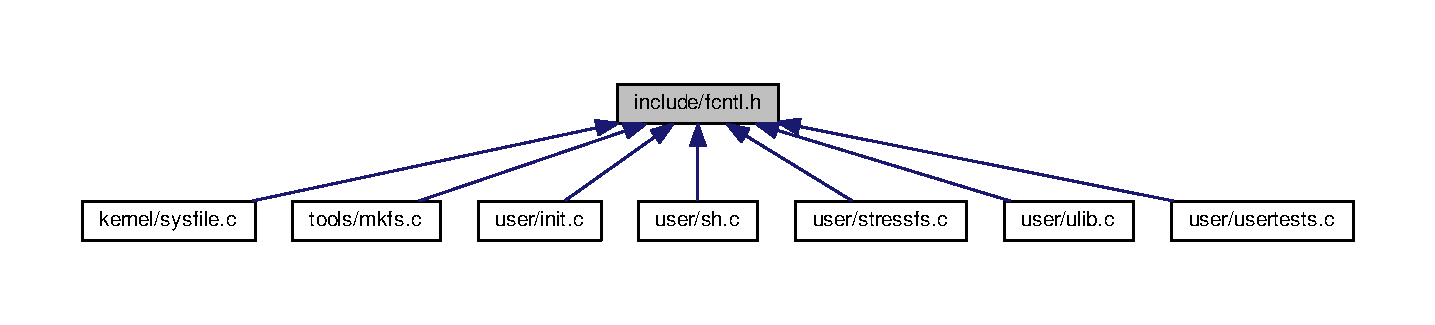
\includegraphics[width=350pt]{fcntl_8h__dep__incl}
\end{center}
\end{figure}
\subsection*{Macros}
\begin{DoxyCompactItemize}
\item 
\#define \hyperlink{fcntl_8h_a7a68c9ffaac7dbcd652225dd7c06a54b}{O\-\_\-\-R\-D\-O\-N\-L\-Y}~0x000
\item 
\#define \hyperlink{fcntl_8h_a11b644a8526139c4cc1850dac1271ced}{O\-\_\-\-W\-R\-O\-N\-L\-Y}~0x001
\item 
\#define \hyperlink{fcntl_8h_abb0586253488ee61072b73557eeb873b}{O\-\_\-\-R\-D\-W\-R}~0x002
\item 
\#define \hyperlink{fcntl_8h_ab40a23079c3b9a7e25ffdc8108c7fb02}{O\-\_\-\-C\-R\-E\-A\-T\-E}~0x200
\end{DoxyCompactItemize}


\subsection{Macro Definition Documentation}
\hypertarget{fcntl_8h_ab40a23079c3b9a7e25ffdc8108c7fb02}{\index{fcntl.\-h@{fcntl.\-h}!O\-\_\-\-C\-R\-E\-A\-T\-E@{O\-\_\-\-C\-R\-E\-A\-T\-E}}
\index{O\-\_\-\-C\-R\-E\-A\-T\-E@{O\-\_\-\-C\-R\-E\-A\-T\-E}!fcntl.h@{fcntl.\-h}}
\subsubsection[{O\-\_\-\-C\-R\-E\-A\-T\-E}]{\setlength{\rightskip}{0pt plus 5cm}\#define O\-\_\-\-C\-R\-E\-A\-T\-E~0x200}}\label{fcntl_8h_ab40a23079c3b9a7e25ffdc8108c7fb02}


Definition at line 9 of file fcntl.\-h.

\hypertarget{fcntl_8h_a7a68c9ffaac7dbcd652225dd7c06a54b}{\index{fcntl.\-h@{fcntl.\-h}!O\-\_\-\-R\-D\-O\-N\-L\-Y@{O\-\_\-\-R\-D\-O\-N\-L\-Y}}
\index{O\-\_\-\-R\-D\-O\-N\-L\-Y@{O\-\_\-\-R\-D\-O\-N\-L\-Y}!fcntl.h@{fcntl.\-h}}
\subsubsection[{O\-\_\-\-R\-D\-O\-N\-L\-Y}]{\setlength{\rightskip}{0pt plus 5cm}\#define O\-\_\-\-R\-D\-O\-N\-L\-Y~0x000}}\label{fcntl_8h_a7a68c9ffaac7dbcd652225dd7c06a54b}


Definition at line 6 of file fcntl.\-h.

\hypertarget{fcntl_8h_abb0586253488ee61072b73557eeb873b}{\index{fcntl.\-h@{fcntl.\-h}!O\-\_\-\-R\-D\-W\-R@{O\-\_\-\-R\-D\-W\-R}}
\index{O\-\_\-\-R\-D\-W\-R@{O\-\_\-\-R\-D\-W\-R}!fcntl.h@{fcntl.\-h}}
\subsubsection[{O\-\_\-\-R\-D\-W\-R}]{\setlength{\rightskip}{0pt plus 5cm}\#define O\-\_\-\-R\-D\-W\-R~0x002}}\label{fcntl_8h_abb0586253488ee61072b73557eeb873b}


Definition at line 8 of file fcntl.\-h.

\hypertarget{fcntl_8h_a11b644a8526139c4cc1850dac1271ced}{\index{fcntl.\-h@{fcntl.\-h}!O\-\_\-\-W\-R\-O\-N\-L\-Y@{O\-\_\-\-W\-R\-O\-N\-L\-Y}}
\index{O\-\_\-\-W\-R\-O\-N\-L\-Y@{O\-\_\-\-W\-R\-O\-N\-L\-Y}!fcntl.h@{fcntl.\-h}}
\subsubsection[{O\-\_\-\-W\-R\-O\-N\-L\-Y}]{\setlength{\rightskip}{0pt plus 5cm}\#define O\-\_\-\-W\-R\-O\-N\-L\-Y~0x001}}\label{fcntl_8h_a11b644a8526139c4cc1850dac1271ced}


Definition at line 7 of file fcntl.\-h.


\hypertarget{fs_8h}{\section{include/fs.h File Reference}
\label{fs_8h}\index{include/fs.\-h@{include/fs.\-h}}
}
This graph shows which files directly or indirectly include this file\-:
\nopagebreak
\begin{figure}[H]
\begin{center}
\leavevmode
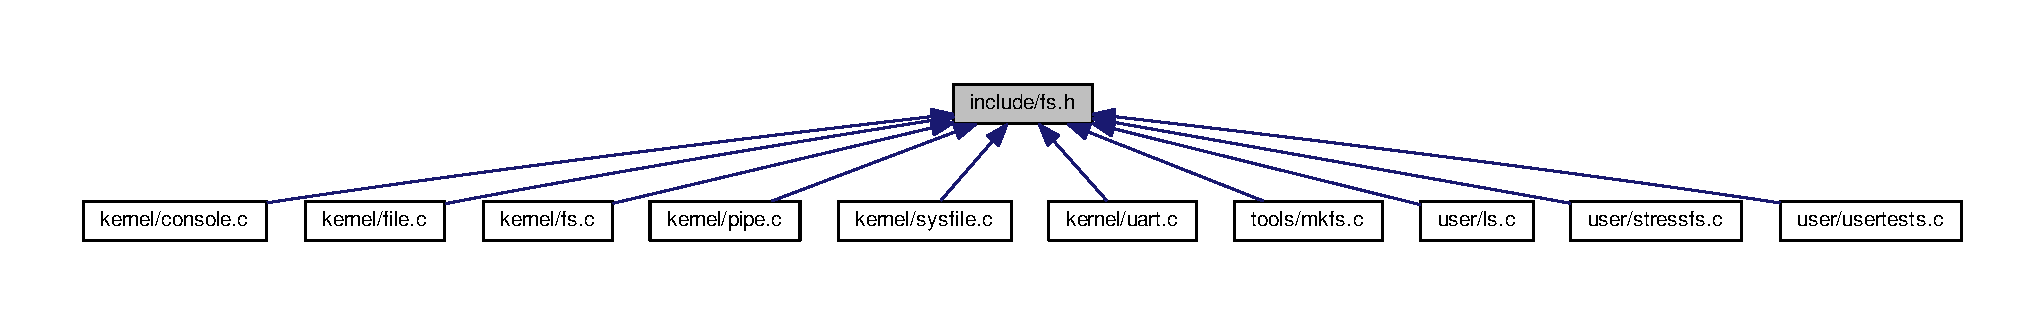
\includegraphics[width=350pt]{fs_8h__dep__incl}
\end{center}
\end{figure}
\subsection*{Data Structures}
\begin{DoxyCompactItemize}
\item 
struct \hyperlink{structsuperblock}{superblock}
\item 
struct \hyperlink{structdinode}{dinode}
\item 
struct \hyperlink{structdirent}{dirent}
\end{DoxyCompactItemize}
\subsection*{Macros}
\begin{DoxyCompactItemize}
\item 
\#define \hyperlink{fs_8h_a22c8ea96d09283ed6496347806cc72a0}{R\-O\-O\-T\-I\-N\-O}~1
\item 
\#define \hyperlink{fs_8h_a403cf3149c084cea115b85c90721039a}{B\-S\-I\-Z\-E}~512
\item 
\#define \hyperlink{fs_8h_acd38e9532d4b3623f844b93c012a8e06}{N\-D\-I\-R\-E\-C\-T}~12
\item 
\#define \hyperlink{fs_8h_a6d24f098ea2928d61ff80b123d761715}{N\-I\-N\-D\-I\-R\-E\-C\-T}~(\hyperlink{fs_8h_a403cf3149c084cea115b85c90721039a}{B\-S\-I\-Z\-E} / sizeof(\hyperlink{types_8h_a91ad9478d81a7aaf2593e8d9c3d06a14}{uint}))
\item 
\#define \hyperlink{fs_8h_a714b2485a6dd312e37226e1f833728a9}{M\-A\-X\-F\-I\-L\-E}~(\hyperlink{fs_8h_acd38e9532d4b3623f844b93c012a8e06}{N\-D\-I\-R\-E\-C\-T} + \hyperlink{fs_8h_a6d24f098ea2928d61ff80b123d761715}{N\-I\-N\-D\-I\-R\-E\-C\-T})
\item 
\#define \hyperlink{fs_8h_aadb6c866a6d0a173f5f0a6ed9c7e0228}{I\-P\-B}~(\hyperlink{fs_8h_a403cf3149c084cea115b85c90721039a}{B\-S\-I\-Z\-E} / sizeof(struct \hyperlink{structdinode}{dinode}))
\item 
\#define \hyperlink{fs_8h_ab114c389e176f9583562c70112425a44}{I\-B\-L\-O\-C\-K}(i)~((i) / \hyperlink{fs_8h_aadb6c866a6d0a173f5f0a6ed9c7e0228}{I\-P\-B} + 2)
\item 
\#define \hyperlink{fs_8h_a3c88fd21abb83ef11461ce750c466828}{B\-P\-B}~(\hyperlink{fs_8h_a403cf3149c084cea115b85c90721039a}{B\-S\-I\-Z\-E}$\ast$8)
\item 
\#define \hyperlink{fs_8h_a3a09a26794f37ae657225b8f4444f368}{B\-B\-L\-O\-C\-K}(b, \hyperlink{mkfs_8c_a2df6f8ae5d8798691d40217c434098e5}{ninodes})~(b/\hyperlink{fs_8h_a3c88fd21abb83ef11461ce750c466828}{B\-P\-B} + (\hyperlink{mkfs_8c_a2df6f8ae5d8798691d40217c434098e5}{ninodes})/\hyperlink{fs_8h_aadb6c866a6d0a173f5f0a6ed9c7e0228}{I\-P\-B} + 3)
\item 
\#define \hyperlink{fs_8h_a48246fb9e5cb7f6a71ebc9ebc2f06562}{D\-I\-R\-S\-I\-Z}~14
\end{DoxyCompactItemize}


\subsection{Macro Definition Documentation}
\hypertarget{fs_8h_a3a09a26794f37ae657225b8f4444f368}{\index{fs.\-h@{fs.\-h}!B\-B\-L\-O\-C\-K@{B\-B\-L\-O\-C\-K}}
\index{B\-B\-L\-O\-C\-K@{B\-B\-L\-O\-C\-K}!fs.h@{fs.\-h}}
\subsubsection[{B\-B\-L\-O\-C\-K}]{\setlength{\rightskip}{0pt plus 5cm}\#define B\-B\-L\-O\-C\-K(
\begin{DoxyParamCaption}
\item[{}]{b, }
\item[{}]{{\bf ninodes}}
\end{DoxyParamCaption}
)~(b/{\bf B\-P\-B} + ({\bf ninodes})/{\bf I\-P\-B} + 3)}}\label{fs_8h_a3a09a26794f37ae657225b8f4444f368}


Definition at line 45 of file fs.\-h.

\hypertarget{fs_8h_a3c88fd21abb83ef11461ce750c466828}{\index{fs.\-h@{fs.\-h}!B\-P\-B@{B\-P\-B}}
\index{B\-P\-B@{B\-P\-B}!fs.h@{fs.\-h}}
\subsubsection[{B\-P\-B}]{\setlength{\rightskip}{0pt plus 5cm}\#define B\-P\-B~({\bf B\-S\-I\-Z\-E}$\ast$8)}}\label{fs_8h_a3c88fd21abb83ef11461ce750c466828}


Definition at line 42 of file fs.\-h.

\hypertarget{fs_8h_a403cf3149c084cea115b85c90721039a}{\index{fs.\-h@{fs.\-h}!B\-S\-I\-Z\-E@{B\-S\-I\-Z\-E}}
\index{B\-S\-I\-Z\-E@{B\-S\-I\-Z\-E}!fs.h@{fs.\-h}}
\subsubsection[{B\-S\-I\-Z\-E}]{\setlength{\rightskip}{0pt plus 5cm}\#define B\-S\-I\-Z\-E~512}}\label{fs_8h_a403cf3149c084cea115b85c90721039a}


Definition at line 12 of file fs.\-h.

\hypertarget{fs_8h_a48246fb9e5cb7f6a71ebc9ebc2f06562}{\index{fs.\-h@{fs.\-h}!D\-I\-R\-S\-I\-Z@{D\-I\-R\-S\-I\-Z}}
\index{D\-I\-R\-S\-I\-Z@{D\-I\-R\-S\-I\-Z}!fs.h@{fs.\-h}}
\subsubsection[{D\-I\-R\-S\-I\-Z}]{\setlength{\rightskip}{0pt plus 5cm}\#define D\-I\-R\-S\-I\-Z~14}}\label{fs_8h_a48246fb9e5cb7f6a71ebc9ebc2f06562}


Definition at line 48 of file fs.\-h.

\hypertarget{fs_8h_ab114c389e176f9583562c70112425a44}{\index{fs.\-h@{fs.\-h}!I\-B\-L\-O\-C\-K@{I\-B\-L\-O\-C\-K}}
\index{I\-B\-L\-O\-C\-K@{I\-B\-L\-O\-C\-K}!fs.h@{fs.\-h}}
\subsubsection[{I\-B\-L\-O\-C\-K}]{\setlength{\rightskip}{0pt plus 5cm}\#define I\-B\-L\-O\-C\-K(
\begin{DoxyParamCaption}
\item[{}]{i}
\end{DoxyParamCaption}
)~((i) / {\bf I\-P\-B} + 2)}}\label{fs_8h_ab114c389e176f9583562c70112425a44}


Definition at line 39 of file fs.\-h.

\hypertarget{fs_8h_aadb6c866a6d0a173f5f0a6ed9c7e0228}{\index{fs.\-h@{fs.\-h}!I\-P\-B@{I\-P\-B}}
\index{I\-P\-B@{I\-P\-B}!fs.h@{fs.\-h}}
\subsubsection[{I\-P\-B}]{\setlength{\rightskip}{0pt plus 5cm}\#define I\-P\-B~({\bf B\-S\-I\-Z\-E} / sizeof(struct {\bf dinode}))}}\label{fs_8h_aadb6c866a6d0a173f5f0a6ed9c7e0228}


Definition at line 36 of file fs.\-h.

\hypertarget{fs_8h_a714b2485a6dd312e37226e1f833728a9}{\index{fs.\-h@{fs.\-h}!M\-A\-X\-F\-I\-L\-E@{M\-A\-X\-F\-I\-L\-E}}
\index{M\-A\-X\-F\-I\-L\-E@{M\-A\-X\-F\-I\-L\-E}!fs.h@{fs.\-h}}
\subsubsection[{M\-A\-X\-F\-I\-L\-E}]{\setlength{\rightskip}{0pt plus 5cm}\#define M\-A\-X\-F\-I\-L\-E~({\bf N\-D\-I\-R\-E\-C\-T} + {\bf N\-I\-N\-D\-I\-R\-E\-C\-T})}}\label{fs_8h_a714b2485a6dd312e37226e1f833728a9}


Definition at line 23 of file fs.\-h.

\hypertarget{fs_8h_acd38e9532d4b3623f844b93c012a8e06}{\index{fs.\-h@{fs.\-h}!N\-D\-I\-R\-E\-C\-T@{N\-D\-I\-R\-E\-C\-T}}
\index{N\-D\-I\-R\-E\-C\-T@{N\-D\-I\-R\-E\-C\-T}!fs.h@{fs.\-h}}
\subsubsection[{N\-D\-I\-R\-E\-C\-T}]{\setlength{\rightskip}{0pt plus 5cm}\#define N\-D\-I\-R\-E\-C\-T~12}}\label{fs_8h_acd38e9532d4b3623f844b93c012a8e06}


Definition at line 21 of file fs.\-h.

\hypertarget{fs_8h_a6d24f098ea2928d61ff80b123d761715}{\index{fs.\-h@{fs.\-h}!N\-I\-N\-D\-I\-R\-E\-C\-T@{N\-I\-N\-D\-I\-R\-E\-C\-T}}
\index{N\-I\-N\-D\-I\-R\-E\-C\-T@{N\-I\-N\-D\-I\-R\-E\-C\-T}!fs.h@{fs.\-h}}
\subsubsection[{N\-I\-N\-D\-I\-R\-E\-C\-T}]{\setlength{\rightskip}{0pt plus 5cm}\#define N\-I\-N\-D\-I\-R\-E\-C\-T~({\bf B\-S\-I\-Z\-E} / sizeof({\bf uint}))}}\label{fs_8h_a6d24f098ea2928d61ff80b123d761715}


Definition at line 22 of file fs.\-h.

\hypertarget{fs_8h_a22c8ea96d09283ed6496347806cc72a0}{\index{fs.\-h@{fs.\-h}!R\-O\-O\-T\-I\-N\-O@{R\-O\-O\-T\-I\-N\-O}}
\index{R\-O\-O\-T\-I\-N\-O@{R\-O\-O\-T\-I\-N\-O}!fs.h@{fs.\-h}}
\subsubsection[{R\-O\-O\-T\-I\-N\-O}]{\setlength{\rightskip}{0pt plus 5cm}\#define R\-O\-O\-T\-I\-N\-O~1}}\label{fs_8h_a22c8ea96d09283ed6496347806cc72a0}


Definition at line 11 of file fs.\-h.


\hypertarget{param_8h}{\section{include/param.h File Reference}
\label{param_8h}\index{include/param.\-h@{include/param.\-h}}
}
This graph shows which files directly or indirectly include this file\-:
\nopagebreak
\begin{figure}[H]
\begin{center}
\leavevmode
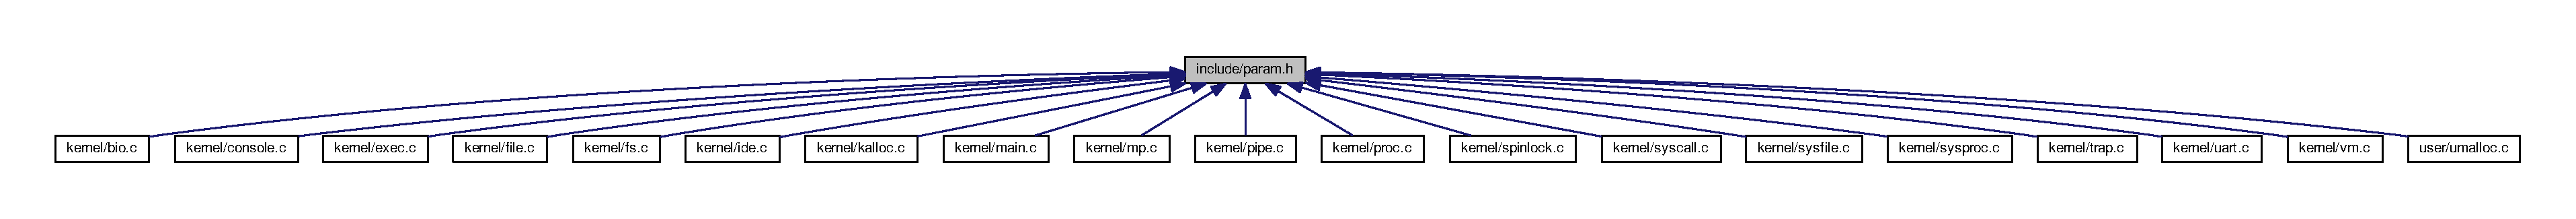
\includegraphics[width=350pt]{param_8h__dep__incl}
\end{center}
\end{figure}
\subsection*{Macros}
\begin{DoxyCompactItemize}
\item 
\#define \hyperlink{param_8h_a810c5b751df5bb30588613ed91095129}{N\-P\-R\-O\-C}~64
\item 
\#define \hyperlink{param_8h_a7735dc19a8cdc3fcafd4241184be4b41}{K\-S\-T\-A\-C\-K\-S\-I\-Z\-E}~4096
\item 
\#define \hyperlink{param_8h_a2c4561c4c17cde39101c4e7a40d4492a}{N\-C\-P\-U}~8
\item 
\#define \hyperlink{param_8h_a80bacbaea8dd6aecf216d85d981bcb21}{N\-O\-F\-I\-L\-E}~16
\item 
\#define \hyperlink{param_8h_a8485f4e81de2537e6a0935626167a775}{N\-F\-I\-L\-E}~100
\item 
\#define \hyperlink{param_8h_ad51e2f8dffd163c263ec676a268d0f0a}{N\-B\-U\-F}~10
\item 
\#define \hyperlink{param_8h_adabafa10c7951be7c875cd2ee212be85}{N\-I\-N\-O\-D\-E}~50
\item 
\#define \hyperlink{param_8h_aa564a41c8409694da49b0badf2bb2853}{N\-D\-E\-V}~10
\item 
\#define \hyperlink{param_8h_ae9ce6b24fe2aae59ff60b469c35febbc}{R\-O\-O\-T\-D\-E\-V}~1
\item 
\#define \hyperlink{param_8h_a0034755b81481716eb7afd61c2b0eee3}{U\-S\-E\-R\-T\-O\-P}~0x\-A0000
\item 
\#define \hyperlink{param_8h_ad3c557a115f7d82d9ef849846779531c}{P\-H\-Y\-S\-T\-O\-P}~0x1000000
\item 
\#define \hyperlink{param_8h_a4c171d1ccc50f0b6ce7ad2f475eeba32}{M\-A\-X\-A\-R\-G}~32
\end{DoxyCompactItemize}


\subsection{Macro Definition Documentation}
\hypertarget{param_8h_a7735dc19a8cdc3fcafd4241184be4b41}{\index{param.\-h@{param.\-h}!K\-S\-T\-A\-C\-K\-S\-I\-Z\-E@{K\-S\-T\-A\-C\-K\-S\-I\-Z\-E}}
\index{K\-S\-T\-A\-C\-K\-S\-I\-Z\-E@{K\-S\-T\-A\-C\-K\-S\-I\-Z\-E}!param.h@{param.\-h}}
\subsubsection[{K\-S\-T\-A\-C\-K\-S\-I\-Z\-E}]{\setlength{\rightskip}{0pt plus 5cm}\#define K\-S\-T\-A\-C\-K\-S\-I\-Z\-E~4096}}\label{param_8h_a7735dc19a8cdc3fcafd4241184be4b41}


Definition at line 7 of file param.\-h.

\hypertarget{param_8h_a4c171d1ccc50f0b6ce7ad2f475eeba32}{\index{param.\-h@{param.\-h}!M\-A\-X\-A\-R\-G@{M\-A\-X\-A\-R\-G}}
\index{M\-A\-X\-A\-R\-G@{M\-A\-X\-A\-R\-G}!param.h@{param.\-h}}
\subsubsection[{M\-A\-X\-A\-R\-G}]{\setlength{\rightskip}{0pt plus 5cm}\#define M\-A\-X\-A\-R\-G~32}}\label{param_8h_a4c171d1ccc50f0b6ce7ad2f475eeba32}


Definition at line 17 of file param.\-h.

\hypertarget{param_8h_ad51e2f8dffd163c263ec676a268d0f0a}{\index{param.\-h@{param.\-h}!N\-B\-U\-F@{N\-B\-U\-F}}
\index{N\-B\-U\-F@{N\-B\-U\-F}!param.h@{param.\-h}}
\subsubsection[{N\-B\-U\-F}]{\setlength{\rightskip}{0pt plus 5cm}\#define N\-B\-U\-F~10}}\label{param_8h_ad51e2f8dffd163c263ec676a268d0f0a}


Definition at line 11 of file param.\-h.

\hypertarget{param_8h_a2c4561c4c17cde39101c4e7a40d4492a}{\index{param.\-h@{param.\-h}!N\-C\-P\-U@{N\-C\-P\-U}}
\index{N\-C\-P\-U@{N\-C\-P\-U}!param.h@{param.\-h}}
\subsubsection[{N\-C\-P\-U}]{\setlength{\rightskip}{0pt plus 5cm}\#define N\-C\-P\-U~8}}\label{param_8h_a2c4561c4c17cde39101c4e7a40d4492a}


Definition at line 8 of file param.\-h.

\hypertarget{param_8h_aa564a41c8409694da49b0badf2bb2853}{\index{param.\-h@{param.\-h}!N\-D\-E\-V@{N\-D\-E\-V}}
\index{N\-D\-E\-V@{N\-D\-E\-V}!param.h@{param.\-h}}
\subsubsection[{N\-D\-E\-V}]{\setlength{\rightskip}{0pt plus 5cm}\#define N\-D\-E\-V~10}}\label{param_8h_aa564a41c8409694da49b0badf2bb2853}


Definition at line 13 of file param.\-h.

\hypertarget{param_8h_a8485f4e81de2537e6a0935626167a775}{\index{param.\-h@{param.\-h}!N\-F\-I\-L\-E@{N\-F\-I\-L\-E}}
\index{N\-F\-I\-L\-E@{N\-F\-I\-L\-E}!param.h@{param.\-h}}
\subsubsection[{N\-F\-I\-L\-E}]{\setlength{\rightskip}{0pt plus 5cm}\#define N\-F\-I\-L\-E~100}}\label{param_8h_a8485f4e81de2537e6a0935626167a775}


Definition at line 10 of file param.\-h.

\hypertarget{param_8h_adabafa10c7951be7c875cd2ee212be85}{\index{param.\-h@{param.\-h}!N\-I\-N\-O\-D\-E@{N\-I\-N\-O\-D\-E}}
\index{N\-I\-N\-O\-D\-E@{N\-I\-N\-O\-D\-E}!param.h@{param.\-h}}
\subsubsection[{N\-I\-N\-O\-D\-E}]{\setlength{\rightskip}{0pt plus 5cm}\#define N\-I\-N\-O\-D\-E~50}}\label{param_8h_adabafa10c7951be7c875cd2ee212be85}


Definition at line 12 of file param.\-h.

\hypertarget{param_8h_a80bacbaea8dd6aecf216d85d981bcb21}{\index{param.\-h@{param.\-h}!N\-O\-F\-I\-L\-E@{N\-O\-F\-I\-L\-E}}
\index{N\-O\-F\-I\-L\-E@{N\-O\-F\-I\-L\-E}!param.h@{param.\-h}}
\subsubsection[{N\-O\-F\-I\-L\-E}]{\setlength{\rightskip}{0pt plus 5cm}\#define N\-O\-F\-I\-L\-E~16}}\label{param_8h_a80bacbaea8dd6aecf216d85d981bcb21}


Definition at line 9 of file param.\-h.

\hypertarget{param_8h_a810c5b751df5bb30588613ed91095129}{\index{param.\-h@{param.\-h}!N\-P\-R\-O\-C@{N\-P\-R\-O\-C}}
\index{N\-P\-R\-O\-C@{N\-P\-R\-O\-C}!param.h@{param.\-h}}
\subsubsection[{N\-P\-R\-O\-C}]{\setlength{\rightskip}{0pt plus 5cm}\#define N\-P\-R\-O\-C~64}}\label{param_8h_a810c5b751df5bb30588613ed91095129}


Definition at line 6 of file param.\-h.

\hypertarget{param_8h_ad3c557a115f7d82d9ef849846779531c}{\index{param.\-h@{param.\-h}!P\-H\-Y\-S\-T\-O\-P@{P\-H\-Y\-S\-T\-O\-P}}
\index{P\-H\-Y\-S\-T\-O\-P@{P\-H\-Y\-S\-T\-O\-P}!param.h@{param.\-h}}
\subsubsection[{P\-H\-Y\-S\-T\-O\-P}]{\setlength{\rightskip}{0pt plus 5cm}\#define P\-H\-Y\-S\-T\-O\-P~0x1000000}}\label{param_8h_ad3c557a115f7d82d9ef849846779531c}


Definition at line 16 of file param.\-h.

\hypertarget{param_8h_ae9ce6b24fe2aae59ff60b469c35febbc}{\index{param.\-h@{param.\-h}!R\-O\-O\-T\-D\-E\-V@{R\-O\-O\-T\-D\-E\-V}}
\index{R\-O\-O\-T\-D\-E\-V@{R\-O\-O\-T\-D\-E\-V}!param.h@{param.\-h}}
\subsubsection[{R\-O\-O\-T\-D\-E\-V}]{\setlength{\rightskip}{0pt plus 5cm}\#define R\-O\-O\-T\-D\-E\-V~1}}\label{param_8h_ae9ce6b24fe2aae59ff60b469c35febbc}


Definition at line 14 of file param.\-h.

\hypertarget{param_8h_a0034755b81481716eb7afd61c2b0eee3}{\index{param.\-h@{param.\-h}!U\-S\-E\-R\-T\-O\-P@{U\-S\-E\-R\-T\-O\-P}}
\index{U\-S\-E\-R\-T\-O\-P@{U\-S\-E\-R\-T\-O\-P}!param.h@{param.\-h}}
\subsubsection[{U\-S\-E\-R\-T\-O\-P}]{\setlength{\rightskip}{0pt plus 5cm}\#define U\-S\-E\-R\-T\-O\-P~0x\-A0000}}\label{param_8h_a0034755b81481716eb7afd61c2b0eee3}


Definition at line 15 of file param.\-h.


\hypertarget{stat_8h}{\section{include/stat.h File Reference}
\label{stat_8h}\index{include/stat.\-h@{include/stat.\-h}}
}
This graph shows which files directly or indirectly include this file\-:
\nopagebreak
\begin{figure}[H]
\begin{center}
\leavevmode
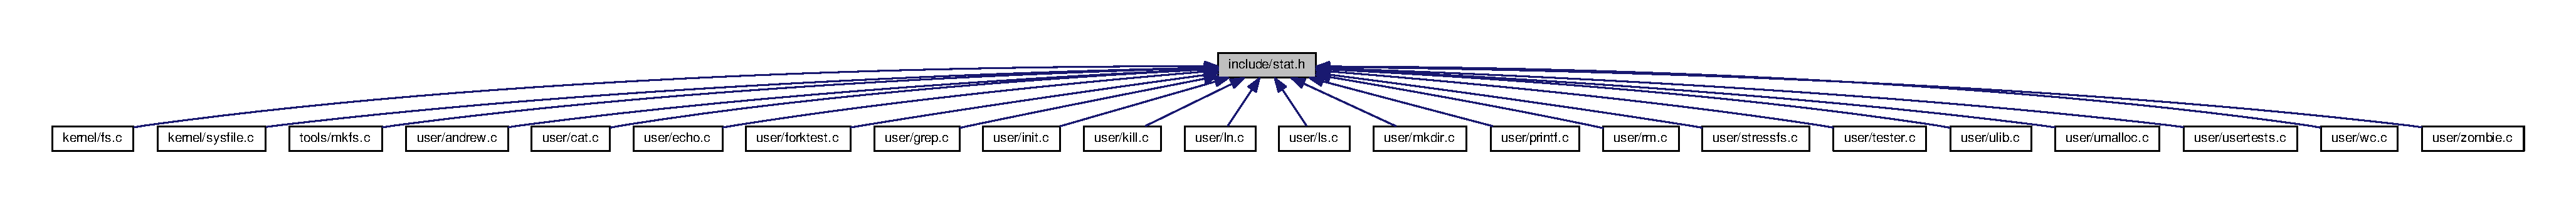
\includegraphics[width=350pt]{stat_8h__dep__incl}
\end{center}
\end{figure}
\subsection*{Data Structures}
\begin{DoxyCompactItemize}
\item 
struct \hyperlink{structstat}{stat}
\end{DoxyCompactItemize}
\subsection*{Macros}
\begin{DoxyCompactItemize}
\item 
\#define \hyperlink{stat_8h_a91136bcd71a9f499304f5d7e7e9d6376}{T\-\_\-\-D\-I\-R}~1
\item 
\#define \hyperlink{stat_8h_a0a8afbed81f5fb3930e9d153fbd51737}{T\-\_\-\-F\-I\-L\-E}~2
\item 
\#define \hyperlink{stat_8h_a62b045a3e4fdf204bdddda0f3fc3d8c4}{T\-\_\-\-D\-E\-V}~3
\end{DoxyCompactItemize}


\subsection{Macro Definition Documentation}
\hypertarget{stat_8h_a62b045a3e4fdf204bdddda0f3fc3d8c4}{\index{stat.\-h@{stat.\-h}!T\-\_\-\-D\-E\-V@{T\-\_\-\-D\-E\-V}}
\index{T\-\_\-\-D\-E\-V@{T\-\_\-\-D\-E\-V}!stat.h@{stat.\-h}}
\subsubsection[{T\-\_\-\-D\-E\-V}]{\setlength{\rightskip}{0pt plus 5cm}\#define T\-\_\-\-D\-E\-V~3}}\label{stat_8h_a62b045a3e4fdf204bdddda0f3fc3d8c4}


Definition at line 8 of file stat.\-h.

\hypertarget{stat_8h_a91136bcd71a9f499304f5d7e7e9d6376}{\index{stat.\-h@{stat.\-h}!T\-\_\-\-D\-I\-R@{T\-\_\-\-D\-I\-R}}
\index{T\-\_\-\-D\-I\-R@{T\-\_\-\-D\-I\-R}!stat.h@{stat.\-h}}
\subsubsection[{T\-\_\-\-D\-I\-R}]{\setlength{\rightskip}{0pt plus 5cm}\#define T\-\_\-\-D\-I\-R~1}}\label{stat_8h_a91136bcd71a9f499304f5d7e7e9d6376}


Definition at line 6 of file stat.\-h.

\hypertarget{stat_8h_a0a8afbed81f5fb3930e9d153fbd51737}{\index{stat.\-h@{stat.\-h}!T\-\_\-\-F\-I\-L\-E@{T\-\_\-\-F\-I\-L\-E}}
\index{T\-\_\-\-F\-I\-L\-E@{T\-\_\-\-F\-I\-L\-E}!stat.h@{stat.\-h}}
\subsubsection[{T\-\_\-\-F\-I\-L\-E}]{\setlength{\rightskip}{0pt plus 5cm}\#define T\-\_\-\-F\-I\-L\-E~2}}\label{stat_8h_a0a8afbed81f5fb3930e9d153fbd51737}


Definition at line 7 of file stat.\-h.


\hypertarget{syscall_8h}{\section{include/syscall.h File Reference}
\label{syscall_8h}\index{include/syscall.\-h@{include/syscall.\-h}}
}
This graph shows which files directly or indirectly include this file\-:
\nopagebreak
\begin{figure}[H]
\begin{center}
\leavevmode
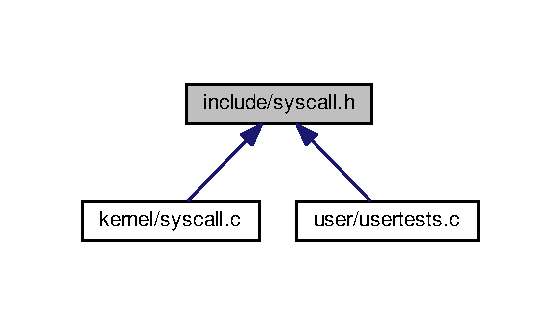
\includegraphics[width=269pt]{syscall_8h__dep__incl}
\end{center}
\end{figure}
\subsection*{Macros}
\begin{DoxyCompactItemize}
\item 
\#define \hyperlink{syscall_8h_a5eba4bd9e19de29f726910510e067d58}{S\-Y\-S\-\_\-fork}~1
\item 
\#define \hyperlink{syscall_8h_a9ffbbdd04d43fb4c0d05d4363d351772}{S\-Y\-S\-\_\-exit}~2
\item 
\#define \hyperlink{syscall_8h_ad8fac614fe5ff393700eba18c0a1e75a}{S\-Y\-S\-\_\-wait}~3
\item 
\#define \hyperlink{syscall_8h_a780e0cccccb5dc0b1a6145c878c5004d}{S\-Y\-S\-\_\-pipe}~4
\item 
\#define \hyperlink{syscall_8h_aa7425a6f80dc9c0ec789079cb6547542}{S\-Y\-S\-\_\-write}~5
\item 
\#define \hyperlink{syscall_8h_a4481bc3f0d65944cd6a9ecd6c5b93a55}{S\-Y\-S\-\_\-read}~6
\item 
\#define \hyperlink{syscall_8h_a8ac7ddcf0e4789f3e705f35b8da40af3}{S\-Y\-S\-\_\-close}~7
\item 
\#define \hyperlink{syscall_8h_ae72be7145975bab983df852500f507f4}{S\-Y\-S\-\_\-kill}~8
\item 
\#define \hyperlink{syscall_8h_a3672b4a5863177cfdf4989e1f3a634b5}{S\-Y\-S\-\_\-exec}~9
\item 
\#define \hyperlink{syscall_8h_a3ba1dfe32baa7a51d8d45fd412d08b91}{S\-Y\-S\-\_\-open}~10
\item 
\#define \hyperlink{syscall_8h_a8da465de7045beb2e558bd601e946c1e}{S\-Y\-S\-\_\-mknod}~11
\item 
\#define \hyperlink{syscall_8h_aa968942341544d4bb806d11c7763e227}{S\-Y\-S\-\_\-unlink}~12
\item 
\#define \hyperlink{syscall_8h_a71105a873ad172a54a16aa2f2d85534a}{S\-Y\-S\-\_\-fstat}~13
\item 
\#define \hyperlink{syscall_8h_a83209641ae7dbc27802761fde434ae5b}{S\-Y\-S\-\_\-link}~14
\item 
\#define \hyperlink{syscall_8h_a0b150013ad6fdc06e94a89c44cc4e780}{S\-Y\-S\-\_\-mkdir}~15
\item 
\#define \hyperlink{syscall_8h_a02542ea0a822502c309e22863d71b849}{S\-Y\-S\-\_\-chdir}~16
\item 
\#define \hyperlink{syscall_8h_a6e98a8f905993a259782ac57a85dbcfc}{S\-Y\-S\-\_\-dup}~17
\item 
\#define \hyperlink{syscall_8h_a7e0844c7709356d697013151cf51c69e}{S\-Y\-S\-\_\-getpid}~18
\item 
\#define \hyperlink{syscall_8h_acceb23729a731ccd9c3ebd6f887b7256}{S\-Y\-S\-\_\-sbrk}~19
\item 
\#define \hyperlink{syscall_8h_a77eac7fe66c659f7731cda964a7ce3dc}{S\-Y\-S\-\_\-sleep}~20
\item 
\#define \hyperlink{syscall_8h_aafb554720ef5628c963c542258b1f639}{S\-Y\-S\-\_\-uptime}~21
\end{DoxyCompactItemize}


\subsection{Macro Definition Documentation}
\hypertarget{syscall_8h_a02542ea0a822502c309e22863d71b849}{\index{syscall.\-h@{syscall.\-h}!S\-Y\-S\-\_\-chdir@{S\-Y\-S\-\_\-chdir}}
\index{S\-Y\-S\-\_\-chdir@{S\-Y\-S\-\_\-chdir}!syscall.h@{syscall.\-h}}
\subsubsection[{S\-Y\-S\-\_\-chdir}]{\setlength{\rightskip}{0pt plus 5cm}\#define S\-Y\-S\-\_\-chdir~16}}\label{syscall_8h_a02542ea0a822502c309e22863d71b849}


Definition at line 20 of file syscall.\-h.

\hypertarget{syscall_8h_a8ac7ddcf0e4789f3e705f35b8da40af3}{\index{syscall.\-h@{syscall.\-h}!S\-Y\-S\-\_\-close@{S\-Y\-S\-\_\-close}}
\index{S\-Y\-S\-\_\-close@{S\-Y\-S\-\_\-close}!syscall.h@{syscall.\-h}}
\subsubsection[{S\-Y\-S\-\_\-close}]{\setlength{\rightskip}{0pt plus 5cm}\#define S\-Y\-S\-\_\-close~7}}\label{syscall_8h_a8ac7ddcf0e4789f3e705f35b8da40af3}


Definition at line 11 of file syscall.\-h.

\hypertarget{syscall_8h_a6e98a8f905993a259782ac57a85dbcfc}{\index{syscall.\-h@{syscall.\-h}!S\-Y\-S\-\_\-dup@{S\-Y\-S\-\_\-dup}}
\index{S\-Y\-S\-\_\-dup@{S\-Y\-S\-\_\-dup}!syscall.h@{syscall.\-h}}
\subsubsection[{S\-Y\-S\-\_\-dup}]{\setlength{\rightskip}{0pt plus 5cm}\#define S\-Y\-S\-\_\-dup~17}}\label{syscall_8h_a6e98a8f905993a259782ac57a85dbcfc}


Definition at line 21 of file syscall.\-h.

\hypertarget{syscall_8h_a3672b4a5863177cfdf4989e1f3a634b5}{\index{syscall.\-h@{syscall.\-h}!S\-Y\-S\-\_\-exec@{S\-Y\-S\-\_\-exec}}
\index{S\-Y\-S\-\_\-exec@{S\-Y\-S\-\_\-exec}!syscall.h@{syscall.\-h}}
\subsubsection[{S\-Y\-S\-\_\-exec}]{\setlength{\rightskip}{0pt plus 5cm}\#define S\-Y\-S\-\_\-exec~9}}\label{syscall_8h_a3672b4a5863177cfdf4989e1f3a634b5}


Definition at line 13 of file syscall.\-h.

\hypertarget{syscall_8h_a9ffbbdd04d43fb4c0d05d4363d351772}{\index{syscall.\-h@{syscall.\-h}!S\-Y\-S\-\_\-exit@{S\-Y\-S\-\_\-exit}}
\index{S\-Y\-S\-\_\-exit@{S\-Y\-S\-\_\-exit}!syscall.h@{syscall.\-h}}
\subsubsection[{S\-Y\-S\-\_\-exit}]{\setlength{\rightskip}{0pt plus 5cm}\#define S\-Y\-S\-\_\-exit~2}}\label{syscall_8h_a9ffbbdd04d43fb4c0d05d4363d351772}


Definition at line 6 of file syscall.\-h.

\hypertarget{syscall_8h_a5eba4bd9e19de29f726910510e067d58}{\index{syscall.\-h@{syscall.\-h}!S\-Y\-S\-\_\-fork@{S\-Y\-S\-\_\-fork}}
\index{S\-Y\-S\-\_\-fork@{S\-Y\-S\-\_\-fork}!syscall.h@{syscall.\-h}}
\subsubsection[{S\-Y\-S\-\_\-fork}]{\setlength{\rightskip}{0pt plus 5cm}\#define S\-Y\-S\-\_\-fork~1}}\label{syscall_8h_a5eba4bd9e19de29f726910510e067d58}


Definition at line 5 of file syscall.\-h.

\hypertarget{syscall_8h_a71105a873ad172a54a16aa2f2d85534a}{\index{syscall.\-h@{syscall.\-h}!S\-Y\-S\-\_\-fstat@{S\-Y\-S\-\_\-fstat}}
\index{S\-Y\-S\-\_\-fstat@{S\-Y\-S\-\_\-fstat}!syscall.h@{syscall.\-h}}
\subsubsection[{S\-Y\-S\-\_\-fstat}]{\setlength{\rightskip}{0pt plus 5cm}\#define S\-Y\-S\-\_\-fstat~13}}\label{syscall_8h_a71105a873ad172a54a16aa2f2d85534a}


Definition at line 17 of file syscall.\-h.

\hypertarget{syscall_8h_a7e0844c7709356d697013151cf51c69e}{\index{syscall.\-h@{syscall.\-h}!S\-Y\-S\-\_\-getpid@{S\-Y\-S\-\_\-getpid}}
\index{S\-Y\-S\-\_\-getpid@{S\-Y\-S\-\_\-getpid}!syscall.h@{syscall.\-h}}
\subsubsection[{S\-Y\-S\-\_\-getpid}]{\setlength{\rightskip}{0pt plus 5cm}\#define S\-Y\-S\-\_\-getpid~18}}\label{syscall_8h_a7e0844c7709356d697013151cf51c69e}


Definition at line 22 of file syscall.\-h.

\hypertarget{syscall_8h_ae72be7145975bab983df852500f507f4}{\index{syscall.\-h@{syscall.\-h}!S\-Y\-S\-\_\-kill@{S\-Y\-S\-\_\-kill}}
\index{S\-Y\-S\-\_\-kill@{S\-Y\-S\-\_\-kill}!syscall.h@{syscall.\-h}}
\subsubsection[{S\-Y\-S\-\_\-kill}]{\setlength{\rightskip}{0pt plus 5cm}\#define S\-Y\-S\-\_\-kill~8}}\label{syscall_8h_ae72be7145975bab983df852500f507f4}


Definition at line 12 of file syscall.\-h.

\hypertarget{syscall_8h_a83209641ae7dbc27802761fde434ae5b}{\index{syscall.\-h@{syscall.\-h}!S\-Y\-S\-\_\-link@{S\-Y\-S\-\_\-link}}
\index{S\-Y\-S\-\_\-link@{S\-Y\-S\-\_\-link}!syscall.h@{syscall.\-h}}
\subsubsection[{S\-Y\-S\-\_\-link}]{\setlength{\rightskip}{0pt plus 5cm}\#define S\-Y\-S\-\_\-link~14}}\label{syscall_8h_a83209641ae7dbc27802761fde434ae5b}


Definition at line 18 of file syscall.\-h.

\hypertarget{syscall_8h_a0b150013ad6fdc06e94a89c44cc4e780}{\index{syscall.\-h@{syscall.\-h}!S\-Y\-S\-\_\-mkdir@{S\-Y\-S\-\_\-mkdir}}
\index{S\-Y\-S\-\_\-mkdir@{S\-Y\-S\-\_\-mkdir}!syscall.h@{syscall.\-h}}
\subsubsection[{S\-Y\-S\-\_\-mkdir}]{\setlength{\rightskip}{0pt plus 5cm}\#define S\-Y\-S\-\_\-mkdir~15}}\label{syscall_8h_a0b150013ad6fdc06e94a89c44cc4e780}


Definition at line 19 of file syscall.\-h.

\hypertarget{syscall_8h_a8da465de7045beb2e558bd601e946c1e}{\index{syscall.\-h@{syscall.\-h}!S\-Y\-S\-\_\-mknod@{S\-Y\-S\-\_\-mknod}}
\index{S\-Y\-S\-\_\-mknod@{S\-Y\-S\-\_\-mknod}!syscall.h@{syscall.\-h}}
\subsubsection[{S\-Y\-S\-\_\-mknod}]{\setlength{\rightskip}{0pt plus 5cm}\#define S\-Y\-S\-\_\-mknod~11}}\label{syscall_8h_a8da465de7045beb2e558bd601e946c1e}


Definition at line 15 of file syscall.\-h.

\hypertarget{syscall_8h_a3ba1dfe32baa7a51d8d45fd412d08b91}{\index{syscall.\-h@{syscall.\-h}!S\-Y\-S\-\_\-open@{S\-Y\-S\-\_\-open}}
\index{S\-Y\-S\-\_\-open@{S\-Y\-S\-\_\-open}!syscall.h@{syscall.\-h}}
\subsubsection[{S\-Y\-S\-\_\-open}]{\setlength{\rightskip}{0pt plus 5cm}\#define S\-Y\-S\-\_\-open~10}}\label{syscall_8h_a3ba1dfe32baa7a51d8d45fd412d08b91}


Definition at line 14 of file syscall.\-h.

\hypertarget{syscall_8h_a780e0cccccb5dc0b1a6145c878c5004d}{\index{syscall.\-h@{syscall.\-h}!S\-Y\-S\-\_\-pipe@{S\-Y\-S\-\_\-pipe}}
\index{S\-Y\-S\-\_\-pipe@{S\-Y\-S\-\_\-pipe}!syscall.h@{syscall.\-h}}
\subsubsection[{S\-Y\-S\-\_\-pipe}]{\setlength{\rightskip}{0pt plus 5cm}\#define S\-Y\-S\-\_\-pipe~4}}\label{syscall_8h_a780e0cccccb5dc0b1a6145c878c5004d}


Definition at line 8 of file syscall.\-h.

\hypertarget{syscall_8h_a4481bc3f0d65944cd6a9ecd6c5b93a55}{\index{syscall.\-h@{syscall.\-h}!S\-Y\-S\-\_\-read@{S\-Y\-S\-\_\-read}}
\index{S\-Y\-S\-\_\-read@{S\-Y\-S\-\_\-read}!syscall.h@{syscall.\-h}}
\subsubsection[{S\-Y\-S\-\_\-read}]{\setlength{\rightskip}{0pt plus 5cm}\#define S\-Y\-S\-\_\-read~6}}\label{syscall_8h_a4481bc3f0d65944cd6a9ecd6c5b93a55}


Definition at line 10 of file syscall.\-h.

\hypertarget{syscall_8h_acceb23729a731ccd9c3ebd6f887b7256}{\index{syscall.\-h@{syscall.\-h}!S\-Y\-S\-\_\-sbrk@{S\-Y\-S\-\_\-sbrk}}
\index{S\-Y\-S\-\_\-sbrk@{S\-Y\-S\-\_\-sbrk}!syscall.h@{syscall.\-h}}
\subsubsection[{S\-Y\-S\-\_\-sbrk}]{\setlength{\rightskip}{0pt plus 5cm}\#define S\-Y\-S\-\_\-sbrk~19}}\label{syscall_8h_acceb23729a731ccd9c3ebd6f887b7256}


Definition at line 23 of file syscall.\-h.

\hypertarget{syscall_8h_a77eac7fe66c659f7731cda964a7ce3dc}{\index{syscall.\-h@{syscall.\-h}!S\-Y\-S\-\_\-sleep@{S\-Y\-S\-\_\-sleep}}
\index{S\-Y\-S\-\_\-sleep@{S\-Y\-S\-\_\-sleep}!syscall.h@{syscall.\-h}}
\subsubsection[{S\-Y\-S\-\_\-sleep}]{\setlength{\rightskip}{0pt plus 5cm}\#define S\-Y\-S\-\_\-sleep~20}}\label{syscall_8h_a77eac7fe66c659f7731cda964a7ce3dc}


Definition at line 24 of file syscall.\-h.

\hypertarget{syscall_8h_aa968942341544d4bb806d11c7763e227}{\index{syscall.\-h@{syscall.\-h}!S\-Y\-S\-\_\-unlink@{S\-Y\-S\-\_\-unlink}}
\index{S\-Y\-S\-\_\-unlink@{S\-Y\-S\-\_\-unlink}!syscall.h@{syscall.\-h}}
\subsubsection[{S\-Y\-S\-\_\-unlink}]{\setlength{\rightskip}{0pt plus 5cm}\#define S\-Y\-S\-\_\-unlink~12}}\label{syscall_8h_aa968942341544d4bb806d11c7763e227}


Definition at line 16 of file syscall.\-h.

\hypertarget{syscall_8h_aafb554720ef5628c963c542258b1f639}{\index{syscall.\-h@{syscall.\-h}!S\-Y\-S\-\_\-uptime@{S\-Y\-S\-\_\-uptime}}
\index{S\-Y\-S\-\_\-uptime@{S\-Y\-S\-\_\-uptime}!syscall.h@{syscall.\-h}}
\subsubsection[{S\-Y\-S\-\_\-uptime}]{\setlength{\rightskip}{0pt plus 5cm}\#define S\-Y\-S\-\_\-uptime~21}}\label{syscall_8h_aafb554720ef5628c963c542258b1f639}


Definition at line 25 of file syscall.\-h.

\hypertarget{syscall_8h_ad8fac614fe5ff393700eba18c0a1e75a}{\index{syscall.\-h@{syscall.\-h}!S\-Y\-S\-\_\-wait@{S\-Y\-S\-\_\-wait}}
\index{S\-Y\-S\-\_\-wait@{S\-Y\-S\-\_\-wait}!syscall.h@{syscall.\-h}}
\subsubsection[{S\-Y\-S\-\_\-wait}]{\setlength{\rightskip}{0pt plus 5cm}\#define S\-Y\-S\-\_\-wait~3}}\label{syscall_8h_ad8fac614fe5ff393700eba18c0a1e75a}


Definition at line 7 of file syscall.\-h.

\hypertarget{syscall_8h_aa7425a6f80dc9c0ec789079cb6547542}{\index{syscall.\-h@{syscall.\-h}!S\-Y\-S\-\_\-write@{S\-Y\-S\-\_\-write}}
\index{S\-Y\-S\-\_\-write@{S\-Y\-S\-\_\-write}!syscall.h@{syscall.\-h}}
\subsubsection[{S\-Y\-S\-\_\-write}]{\setlength{\rightskip}{0pt plus 5cm}\#define S\-Y\-S\-\_\-write~5}}\label{syscall_8h_aa7425a6f80dc9c0ec789079cb6547542}


Definition at line 9 of file syscall.\-h.


\hypertarget{traps_8h}{\section{include/traps.h File Reference}
\label{traps_8h}\index{include/traps.\-h@{include/traps.\-h}}
}
This graph shows which files directly or indirectly include this file\-:
\nopagebreak
\begin{figure}[H]
\begin{center}
\leavevmode
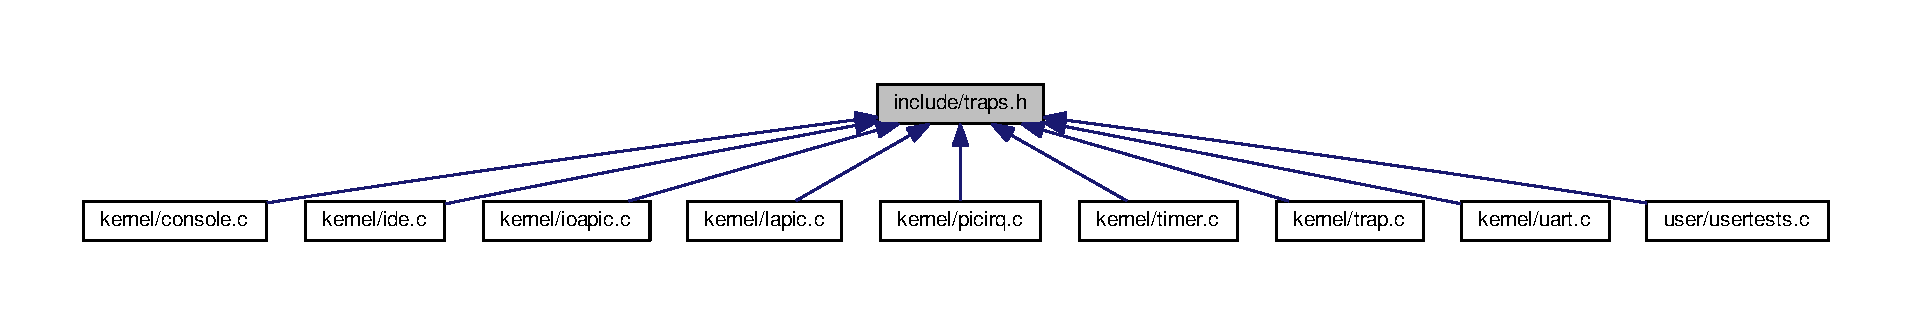
\includegraphics[width=350pt]{traps_8h__dep__incl}
\end{center}
\end{figure}
\subsection*{Macros}
\begin{DoxyCompactItemize}
\item 
\#define \hyperlink{traps_8h_aafec4ddec2a31119ce77162e2d4e126d}{T\-\_\-\-D\-I\-V\-I\-D\-E}~0
\item 
\#define \hyperlink{traps_8h_a7adfcee96fd3df5bc6308209e6fd8947}{T\-\_\-\-D\-E\-B\-U\-G}~1
\item 
\#define \hyperlink{traps_8h_a5549435e3ba47c1e8c2ee1ebbcde9e3c}{T\-\_\-\-N\-M\-I}~2
\item 
\#define \hyperlink{traps_8h_aeb503241653717f4d1d117b6f718fd17}{T\-\_\-\-B\-R\-K\-P\-T}~3
\item 
\#define \hyperlink{traps_8h_aa2d9567ea3f81683de5ccfacac0ee866}{T\-\_\-\-O\-F\-L\-O\-W}~4
\item 
\#define \hyperlink{traps_8h_ac00f437e67ad81b01ae4cc85fc75d4e2}{T\-\_\-\-B\-O\-U\-N\-D}~5
\item 
\#define \hyperlink{traps_8h_ab508bbd71b1eaa5278660be9fcd503a6}{T\-\_\-\-I\-L\-L\-O\-P}~6
\item 
\#define \hyperlink{traps_8h_aef6db5115b3223f8b9b97ec9cfa1d161}{T\-\_\-\-D\-E\-V\-I\-C\-E}~7
\item 
\#define \hyperlink{traps_8h_af1e4d5a54ee4b09367a99565acc33172}{T\-\_\-\-D\-B\-L\-F\-L\-T}~8
\item 
\#define \hyperlink{traps_8h_a547922760445e2906d9168a65d9bb132}{T\-\_\-\-T\-S\-S}~10
\item 
\#define \hyperlink{traps_8h_ad57a595242a4f6a42978dabaa6113ec0}{T\-\_\-\-S\-E\-G\-N\-P}~11
\item 
\#define \hyperlink{traps_8h_acf4cab67d7c76dc6b37ef3a037394d09}{T\-\_\-\-S\-T\-A\-C\-K}~12
\item 
\#define \hyperlink{traps_8h_a62141642981612f78963d6fa5a7f600a}{T\-\_\-\-G\-P\-F\-L\-T}~13
\item 
\#define \hyperlink{traps_8h_a79fafc536ca51352802d69fe3118eead}{T\-\_\-\-P\-G\-F\-L\-T}~14
\item 
\#define \hyperlink{traps_8h_a883155e087e0e436a6e2d734b5bd247b}{T\-\_\-\-F\-P\-E\-R\-R}~16
\item 
\#define \hyperlink{traps_8h_a04b077da4e7bcdaa52e9900e3ac2ad46}{T\-\_\-\-A\-L\-I\-G\-N}~17
\item 
\#define \hyperlink{traps_8h_a39704806098b0fdee2ad18a46c87b5a4}{T\-\_\-\-M\-C\-H\-K}~18
\item 
\#define \hyperlink{traps_8h_a009bee02b7ee62856b8662d16d12dea3}{T\-\_\-\-S\-I\-M\-D\-E\-R\-R}~19
\item 
\#define \hyperlink{traps_8h_a6914c7173b6fe6d04e78d0876e39d95e}{T\-\_\-\-S\-Y\-S\-C\-A\-L\-L}~64
\item 
\#define \hyperlink{traps_8h_a9b10f19a4f29fd2599888400adc48b0e}{T\-\_\-\-D\-E\-F\-A\-U\-L\-T}~500
\item 
\#define \hyperlink{traps_8h_a17129100154901eb81be6e438843a0e1}{T\-\_\-\-I\-R\-Q0}~32
\item 
\#define \hyperlink{traps_8h_a85fc66e3edd4ed6a4db6e455feaba8ca}{I\-R\-Q\-\_\-\-T\-I\-M\-E\-R}~0
\item 
\#define \hyperlink{traps_8h_a0b7569cda71298859ffb6ea55c03a36a}{I\-R\-Q\-\_\-\-K\-B\-D}~1
\item 
\#define \hyperlink{traps_8h_a603b478f70a928f442e33fefba73494a}{I\-R\-Q\-\_\-\-C\-O\-M1}~4
\item 
\#define \hyperlink{traps_8h_ae17548e9192fbdecfb02247721aaf2df}{I\-R\-Q\-\_\-\-I\-D\-E}~14
\item 
\#define \hyperlink{traps_8h_a7546e682900c4558b1f8c4f0633bc7b9}{I\-R\-Q\-\_\-\-E\-R\-R\-O\-R}~19
\item 
\#define \hyperlink{traps_8h_a0e95f09d5e5653670eede10844d73875}{I\-R\-Q\-\_\-\-S\-P\-U\-R\-I\-O\-U\-S}~31
\end{DoxyCompactItemize}


\subsection{Macro Definition Documentation}
\hypertarget{traps_8h_a603b478f70a928f442e33fefba73494a}{\index{traps.\-h@{traps.\-h}!I\-R\-Q\-\_\-\-C\-O\-M1@{I\-R\-Q\-\_\-\-C\-O\-M1}}
\index{I\-R\-Q\-\_\-\-C\-O\-M1@{I\-R\-Q\-\_\-\-C\-O\-M1}!traps.h@{traps.\-h}}
\subsubsection[{I\-R\-Q\-\_\-\-C\-O\-M1}]{\setlength{\rightskip}{0pt plus 5cm}\#define I\-R\-Q\-\_\-\-C\-O\-M1~4}}\label{traps_8h_a603b478f70a928f442e33fefba73494a}


Definition at line 37 of file traps.\-h.

\hypertarget{traps_8h_a7546e682900c4558b1f8c4f0633bc7b9}{\index{traps.\-h@{traps.\-h}!I\-R\-Q\-\_\-\-E\-R\-R\-O\-R@{I\-R\-Q\-\_\-\-E\-R\-R\-O\-R}}
\index{I\-R\-Q\-\_\-\-E\-R\-R\-O\-R@{I\-R\-Q\-\_\-\-E\-R\-R\-O\-R}!traps.h@{traps.\-h}}
\subsubsection[{I\-R\-Q\-\_\-\-E\-R\-R\-O\-R}]{\setlength{\rightskip}{0pt plus 5cm}\#define I\-R\-Q\-\_\-\-E\-R\-R\-O\-R~19}}\label{traps_8h_a7546e682900c4558b1f8c4f0633bc7b9}


Definition at line 39 of file traps.\-h.

\hypertarget{traps_8h_ae17548e9192fbdecfb02247721aaf2df}{\index{traps.\-h@{traps.\-h}!I\-R\-Q\-\_\-\-I\-D\-E@{I\-R\-Q\-\_\-\-I\-D\-E}}
\index{I\-R\-Q\-\_\-\-I\-D\-E@{I\-R\-Q\-\_\-\-I\-D\-E}!traps.h@{traps.\-h}}
\subsubsection[{I\-R\-Q\-\_\-\-I\-D\-E}]{\setlength{\rightskip}{0pt plus 5cm}\#define I\-R\-Q\-\_\-\-I\-D\-E~14}}\label{traps_8h_ae17548e9192fbdecfb02247721aaf2df}


Definition at line 38 of file traps.\-h.

\hypertarget{traps_8h_a0b7569cda71298859ffb6ea55c03a36a}{\index{traps.\-h@{traps.\-h}!I\-R\-Q\-\_\-\-K\-B\-D@{I\-R\-Q\-\_\-\-K\-B\-D}}
\index{I\-R\-Q\-\_\-\-K\-B\-D@{I\-R\-Q\-\_\-\-K\-B\-D}!traps.h@{traps.\-h}}
\subsubsection[{I\-R\-Q\-\_\-\-K\-B\-D}]{\setlength{\rightskip}{0pt plus 5cm}\#define I\-R\-Q\-\_\-\-K\-B\-D~1}}\label{traps_8h_a0b7569cda71298859ffb6ea55c03a36a}


Definition at line 36 of file traps.\-h.

\hypertarget{traps_8h_a0e95f09d5e5653670eede10844d73875}{\index{traps.\-h@{traps.\-h}!I\-R\-Q\-\_\-\-S\-P\-U\-R\-I\-O\-U\-S@{I\-R\-Q\-\_\-\-S\-P\-U\-R\-I\-O\-U\-S}}
\index{I\-R\-Q\-\_\-\-S\-P\-U\-R\-I\-O\-U\-S@{I\-R\-Q\-\_\-\-S\-P\-U\-R\-I\-O\-U\-S}!traps.h@{traps.\-h}}
\subsubsection[{I\-R\-Q\-\_\-\-S\-P\-U\-R\-I\-O\-U\-S}]{\setlength{\rightskip}{0pt plus 5cm}\#define I\-R\-Q\-\_\-\-S\-P\-U\-R\-I\-O\-U\-S~31}}\label{traps_8h_a0e95f09d5e5653670eede10844d73875}


Definition at line 40 of file traps.\-h.

\hypertarget{traps_8h_a85fc66e3edd4ed6a4db6e455feaba8ca}{\index{traps.\-h@{traps.\-h}!I\-R\-Q\-\_\-\-T\-I\-M\-E\-R@{I\-R\-Q\-\_\-\-T\-I\-M\-E\-R}}
\index{I\-R\-Q\-\_\-\-T\-I\-M\-E\-R@{I\-R\-Q\-\_\-\-T\-I\-M\-E\-R}!traps.h@{traps.\-h}}
\subsubsection[{I\-R\-Q\-\_\-\-T\-I\-M\-E\-R}]{\setlength{\rightskip}{0pt plus 5cm}\#define I\-R\-Q\-\_\-\-T\-I\-M\-E\-R~0}}\label{traps_8h_a85fc66e3edd4ed6a4db6e455feaba8ca}


Definition at line 35 of file traps.\-h.

\hypertarget{traps_8h_a04b077da4e7bcdaa52e9900e3ac2ad46}{\index{traps.\-h@{traps.\-h}!T\-\_\-\-A\-L\-I\-G\-N@{T\-\_\-\-A\-L\-I\-G\-N}}
\index{T\-\_\-\-A\-L\-I\-G\-N@{T\-\_\-\-A\-L\-I\-G\-N}!traps.h@{traps.\-h}}
\subsubsection[{T\-\_\-\-A\-L\-I\-G\-N}]{\setlength{\rightskip}{0pt plus 5cm}\#define T\-\_\-\-A\-L\-I\-G\-N~17}}\label{traps_8h_a04b077da4e7bcdaa52e9900e3ac2ad46}


Definition at line 24 of file traps.\-h.

\hypertarget{traps_8h_ac00f437e67ad81b01ae4cc85fc75d4e2}{\index{traps.\-h@{traps.\-h}!T\-\_\-\-B\-O\-U\-N\-D@{T\-\_\-\-B\-O\-U\-N\-D}}
\index{T\-\_\-\-B\-O\-U\-N\-D@{T\-\_\-\-B\-O\-U\-N\-D}!traps.h@{traps.\-h}}
\subsubsection[{T\-\_\-\-B\-O\-U\-N\-D}]{\setlength{\rightskip}{0pt plus 5cm}\#define T\-\_\-\-B\-O\-U\-N\-D~5}}\label{traps_8h_ac00f437e67ad81b01ae4cc85fc75d4e2}


Definition at line 12 of file traps.\-h.

\hypertarget{traps_8h_aeb503241653717f4d1d117b6f718fd17}{\index{traps.\-h@{traps.\-h}!T\-\_\-\-B\-R\-K\-P\-T@{T\-\_\-\-B\-R\-K\-P\-T}}
\index{T\-\_\-\-B\-R\-K\-P\-T@{T\-\_\-\-B\-R\-K\-P\-T}!traps.h@{traps.\-h}}
\subsubsection[{T\-\_\-\-B\-R\-K\-P\-T}]{\setlength{\rightskip}{0pt plus 5cm}\#define T\-\_\-\-B\-R\-K\-P\-T~3}}\label{traps_8h_aeb503241653717f4d1d117b6f718fd17}


Definition at line 10 of file traps.\-h.

\hypertarget{traps_8h_af1e4d5a54ee4b09367a99565acc33172}{\index{traps.\-h@{traps.\-h}!T\-\_\-\-D\-B\-L\-F\-L\-T@{T\-\_\-\-D\-B\-L\-F\-L\-T}}
\index{T\-\_\-\-D\-B\-L\-F\-L\-T@{T\-\_\-\-D\-B\-L\-F\-L\-T}!traps.h@{traps.\-h}}
\subsubsection[{T\-\_\-\-D\-B\-L\-F\-L\-T}]{\setlength{\rightskip}{0pt plus 5cm}\#define T\-\_\-\-D\-B\-L\-F\-L\-T~8}}\label{traps_8h_af1e4d5a54ee4b09367a99565acc33172}


Definition at line 15 of file traps.\-h.

\hypertarget{traps_8h_a7adfcee96fd3df5bc6308209e6fd8947}{\index{traps.\-h@{traps.\-h}!T\-\_\-\-D\-E\-B\-U\-G@{T\-\_\-\-D\-E\-B\-U\-G}}
\index{T\-\_\-\-D\-E\-B\-U\-G@{T\-\_\-\-D\-E\-B\-U\-G}!traps.h@{traps.\-h}}
\subsubsection[{T\-\_\-\-D\-E\-B\-U\-G}]{\setlength{\rightskip}{0pt plus 5cm}\#define T\-\_\-\-D\-E\-B\-U\-G~1}}\label{traps_8h_a7adfcee96fd3df5bc6308209e6fd8947}


Definition at line 8 of file traps.\-h.

\hypertarget{traps_8h_a9b10f19a4f29fd2599888400adc48b0e}{\index{traps.\-h@{traps.\-h}!T\-\_\-\-D\-E\-F\-A\-U\-L\-T@{T\-\_\-\-D\-E\-F\-A\-U\-L\-T}}
\index{T\-\_\-\-D\-E\-F\-A\-U\-L\-T@{T\-\_\-\-D\-E\-F\-A\-U\-L\-T}!traps.h@{traps.\-h}}
\subsubsection[{T\-\_\-\-D\-E\-F\-A\-U\-L\-T}]{\setlength{\rightskip}{0pt plus 5cm}\#define T\-\_\-\-D\-E\-F\-A\-U\-L\-T~500}}\label{traps_8h_a9b10f19a4f29fd2599888400adc48b0e}


Definition at line 31 of file traps.\-h.

\hypertarget{traps_8h_aef6db5115b3223f8b9b97ec9cfa1d161}{\index{traps.\-h@{traps.\-h}!T\-\_\-\-D\-E\-V\-I\-C\-E@{T\-\_\-\-D\-E\-V\-I\-C\-E}}
\index{T\-\_\-\-D\-E\-V\-I\-C\-E@{T\-\_\-\-D\-E\-V\-I\-C\-E}!traps.h@{traps.\-h}}
\subsubsection[{T\-\_\-\-D\-E\-V\-I\-C\-E}]{\setlength{\rightskip}{0pt plus 5cm}\#define T\-\_\-\-D\-E\-V\-I\-C\-E~7}}\label{traps_8h_aef6db5115b3223f8b9b97ec9cfa1d161}


Definition at line 14 of file traps.\-h.

\hypertarget{traps_8h_aafec4ddec2a31119ce77162e2d4e126d}{\index{traps.\-h@{traps.\-h}!T\-\_\-\-D\-I\-V\-I\-D\-E@{T\-\_\-\-D\-I\-V\-I\-D\-E}}
\index{T\-\_\-\-D\-I\-V\-I\-D\-E@{T\-\_\-\-D\-I\-V\-I\-D\-E}!traps.h@{traps.\-h}}
\subsubsection[{T\-\_\-\-D\-I\-V\-I\-D\-E}]{\setlength{\rightskip}{0pt plus 5cm}\#define T\-\_\-\-D\-I\-V\-I\-D\-E~0}}\label{traps_8h_aafec4ddec2a31119ce77162e2d4e126d}


Definition at line 7 of file traps.\-h.

\hypertarget{traps_8h_a883155e087e0e436a6e2d734b5bd247b}{\index{traps.\-h@{traps.\-h}!T\-\_\-\-F\-P\-E\-R\-R@{T\-\_\-\-F\-P\-E\-R\-R}}
\index{T\-\_\-\-F\-P\-E\-R\-R@{T\-\_\-\-F\-P\-E\-R\-R}!traps.h@{traps.\-h}}
\subsubsection[{T\-\_\-\-F\-P\-E\-R\-R}]{\setlength{\rightskip}{0pt plus 5cm}\#define T\-\_\-\-F\-P\-E\-R\-R~16}}\label{traps_8h_a883155e087e0e436a6e2d734b5bd247b}


Definition at line 23 of file traps.\-h.

\hypertarget{traps_8h_a62141642981612f78963d6fa5a7f600a}{\index{traps.\-h@{traps.\-h}!T\-\_\-\-G\-P\-F\-L\-T@{T\-\_\-\-G\-P\-F\-L\-T}}
\index{T\-\_\-\-G\-P\-F\-L\-T@{T\-\_\-\-G\-P\-F\-L\-T}!traps.h@{traps.\-h}}
\subsubsection[{T\-\_\-\-G\-P\-F\-L\-T}]{\setlength{\rightskip}{0pt plus 5cm}\#define T\-\_\-\-G\-P\-F\-L\-T~13}}\label{traps_8h_a62141642981612f78963d6fa5a7f600a}


Definition at line 20 of file traps.\-h.

\hypertarget{traps_8h_ab508bbd71b1eaa5278660be9fcd503a6}{\index{traps.\-h@{traps.\-h}!T\-\_\-\-I\-L\-L\-O\-P@{T\-\_\-\-I\-L\-L\-O\-P}}
\index{T\-\_\-\-I\-L\-L\-O\-P@{T\-\_\-\-I\-L\-L\-O\-P}!traps.h@{traps.\-h}}
\subsubsection[{T\-\_\-\-I\-L\-L\-O\-P}]{\setlength{\rightskip}{0pt plus 5cm}\#define T\-\_\-\-I\-L\-L\-O\-P~6}}\label{traps_8h_ab508bbd71b1eaa5278660be9fcd503a6}


Definition at line 13 of file traps.\-h.

\hypertarget{traps_8h_a17129100154901eb81be6e438843a0e1}{\index{traps.\-h@{traps.\-h}!T\-\_\-\-I\-R\-Q0@{T\-\_\-\-I\-R\-Q0}}
\index{T\-\_\-\-I\-R\-Q0@{T\-\_\-\-I\-R\-Q0}!traps.h@{traps.\-h}}
\subsubsection[{T\-\_\-\-I\-R\-Q0}]{\setlength{\rightskip}{0pt plus 5cm}\#define T\-\_\-\-I\-R\-Q0~32}}\label{traps_8h_a17129100154901eb81be6e438843a0e1}


Definition at line 33 of file traps.\-h.

\hypertarget{traps_8h_a39704806098b0fdee2ad18a46c87b5a4}{\index{traps.\-h@{traps.\-h}!T\-\_\-\-M\-C\-H\-K@{T\-\_\-\-M\-C\-H\-K}}
\index{T\-\_\-\-M\-C\-H\-K@{T\-\_\-\-M\-C\-H\-K}!traps.h@{traps.\-h}}
\subsubsection[{T\-\_\-\-M\-C\-H\-K}]{\setlength{\rightskip}{0pt plus 5cm}\#define T\-\_\-\-M\-C\-H\-K~18}}\label{traps_8h_a39704806098b0fdee2ad18a46c87b5a4}


Definition at line 25 of file traps.\-h.

\hypertarget{traps_8h_a5549435e3ba47c1e8c2ee1ebbcde9e3c}{\index{traps.\-h@{traps.\-h}!T\-\_\-\-N\-M\-I@{T\-\_\-\-N\-M\-I}}
\index{T\-\_\-\-N\-M\-I@{T\-\_\-\-N\-M\-I}!traps.h@{traps.\-h}}
\subsubsection[{T\-\_\-\-N\-M\-I}]{\setlength{\rightskip}{0pt plus 5cm}\#define T\-\_\-\-N\-M\-I~2}}\label{traps_8h_a5549435e3ba47c1e8c2ee1ebbcde9e3c}


Definition at line 9 of file traps.\-h.

\hypertarget{traps_8h_aa2d9567ea3f81683de5ccfacac0ee866}{\index{traps.\-h@{traps.\-h}!T\-\_\-\-O\-F\-L\-O\-W@{T\-\_\-\-O\-F\-L\-O\-W}}
\index{T\-\_\-\-O\-F\-L\-O\-W@{T\-\_\-\-O\-F\-L\-O\-W}!traps.h@{traps.\-h}}
\subsubsection[{T\-\_\-\-O\-F\-L\-O\-W}]{\setlength{\rightskip}{0pt plus 5cm}\#define T\-\_\-\-O\-F\-L\-O\-W~4}}\label{traps_8h_aa2d9567ea3f81683de5ccfacac0ee866}


Definition at line 11 of file traps.\-h.

\hypertarget{traps_8h_a79fafc536ca51352802d69fe3118eead}{\index{traps.\-h@{traps.\-h}!T\-\_\-\-P\-G\-F\-L\-T@{T\-\_\-\-P\-G\-F\-L\-T}}
\index{T\-\_\-\-P\-G\-F\-L\-T@{T\-\_\-\-P\-G\-F\-L\-T}!traps.h@{traps.\-h}}
\subsubsection[{T\-\_\-\-P\-G\-F\-L\-T}]{\setlength{\rightskip}{0pt plus 5cm}\#define T\-\_\-\-P\-G\-F\-L\-T~14}}\label{traps_8h_a79fafc536ca51352802d69fe3118eead}


Definition at line 21 of file traps.\-h.

\hypertarget{traps_8h_ad57a595242a4f6a42978dabaa6113ec0}{\index{traps.\-h@{traps.\-h}!T\-\_\-\-S\-E\-G\-N\-P@{T\-\_\-\-S\-E\-G\-N\-P}}
\index{T\-\_\-\-S\-E\-G\-N\-P@{T\-\_\-\-S\-E\-G\-N\-P}!traps.h@{traps.\-h}}
\subsubsection[{T\-\_\-\-S\-E\-G\-N\-P}]{\setlength{\rightskip}{0pt plus 5cm}\#define T\-\_\-\-S\-E\-G\-N\-P~11}}\label{traps_8h_ad57a595242a4f6a42978dabaa6113ec0}


Definition at line 18 of file traps.\-h.

\hypertarget{traps_8h_a009bee02b7ee62856b8662d16d12dea3}{\index{traps.\-h@{traps.\-h}!T\-\_\-\-S\-I\-M\-D\-E\-R\-R@{T\-\_\-\-S\-I\-M\-D\-E\-R\-R}}
\index{T\-\_\-\-S\-I\-M\-D\-E\-R\-R@{T\-\_\-\-S\-I\-M\-D\-E\-R\-R}!traps.h@{traps.\-h}}
\subsubsection[{T\-\_\-\-S\-I\-M\-D\-E\-R\-R}]{\setlength{\rightskip}{0pt plus 5cm}\#define T\-\_\-\-S\-I\-M\-D\-E\-R\-R~19}}\label{traps_8h_a009bee02b7ee62856b8662d16d12dea3}


Definition at line 26 of file traps.\-h.

\hypertarget{traps_8h_acf4cab67d7c76dc6b37ef3a037394d09}{\index{traps.\-h@{traps.\-h}!T\-\_\-\-S\-T\-A\-C\-K@{T\-\_\-\-S\-T\-A\-C\-K}}
\index{T\-\_\-\-S\-T\-A\-C\-K@{T\-\_\-\-S\-T\-A\-C\-K}!traps.h@{traps.\-h}}
\subsubsection[{T\-\_\-\-S\-T\-A\-C\-K}]{\setlength{\rightskip}{0pt plus 5cm}\#define T\-\_\-\-S\-T\-A\-C\-K~12}}\label{traps_8h_acf4cab67d7c76dc6b37ef3a037394d09}


Definition at line 19 of file traps.\-h.

\hypertarget{traps_8h_a6914c7173b6fe6d04e78d0876e39d95e}{\index{traps.\-h@{traps.\-h}!T\-\_\-\-S\-Y\-S\-C\-A\-L\-L@{T\-\_\-\-S\-Y\-S\-C\-A\-L\-L}}
\index{T\-\_\-\-S\-Y\-S\-C\-A\-L\-L@{T\-\_\-\-S\-Y\-S\-C\-A\-L\-L}!traps.h@{traps.\-h}}
\subsubsection[{T\-\_\-\-S\-Y\-S\-C\-A\-L\-L}]{\setlength{\rightskip}{0pt plus 5cm}\#define T\-\_\-\-S\-Y\-S\-C\-A\-L\-L~64}}\label{traps_8h_a6914c7173b6fe6d04e78d0876e39d95e}


Definition at line 30 of file traps.\-h.

\hypertarget{traps_8h_a547922760445e2906d9168a65d9bb132}{\index{traps.\-h@{traps.\-h}!T\-\_\-\-T\-S\-S@{T\-\_\-\-T\-S\-S}}
\index{T\-\_\-\-T\-S\-S@{T\-\_\-\-T\-S\-S}!traps.h@{traps.\-h}}
\subsubsection[{T\-\_\-\-T\-S\-S}]{\setlength{\rightskip}{0pt plus 5cm}\#define T\-\_\-\-T\-S\-S~10}}\label{traps_8h_a547922760445e2906d9168a65d9bb132}


Definition at line 17 of file traps.\-h.


\hypertarget{types_8h}{\section{include/types.h File Reference}
\label{types_8h}\index{include/types.\-h@{include/types.\-h}}
}
This graph shows which files directly or indirectly include this file\-:
\nopagebreak
\begin{figure}[H]
\begin{center}
\leavevmode
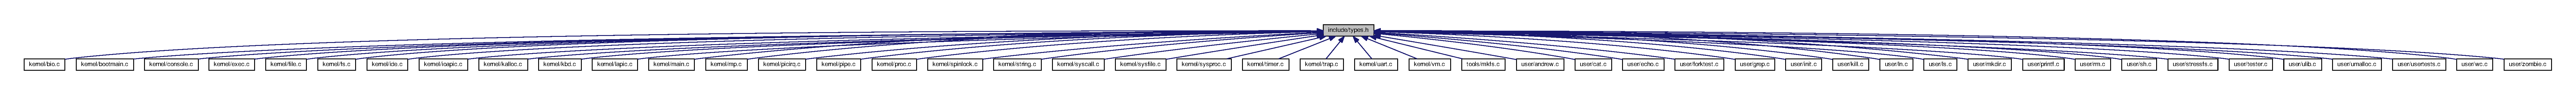
\includegraphics[width=350pt]{types_8h__dep__incl}
\end{center}
\end{figure}
\subsection*{Macros}
\begin{DoxyCompactItemize}
\item 
\#define \hyperlink{types_8h_a070d2ce7b6bb7e5c05602aa8c308d0c4}{N\-U\-L\-L}~(0)
\end{DoxyCompactItemize}
\subsection*{Typedefs}
\begin{DoxyCompactItemize}
\item 
typedef unsigned int \hyperlink{types_8h_a91ad9478d81a7aaf2593e8d9c3d06a14}{uint}
\item 
typedef unsigned short \hyperlink{types_8h_ab95f123a6c9bcfee6a343170ef8c5f69}{ushort}
\item 
typedef unsigned char \hyperlink{types_8h_a65f85814a8290f9797005d3b28e7e5fc}{uchar}
\item 
typedef \hyperlink{types_8h_a91ad9478d81a7aaf2593e8d9c3d06a14}{uint} \hyperlink{types_8h_ac131849542282b2c95dfeaf1f26dc010}{pde\-\_\-t}
\end{DoxyCompactItemize}


\subsection{Macro Definition Documentation}
\hypertarget{types_8h_a070d2ce7b6bb7e5c05602aa8c308d0c4}{\index{types.\-h@{types.\-h}!N\-U\-L\-L@{N\-U\-L\-L}}
\index{N\-U\-L\-L@{N\-U\-L\-L}!types.h@{types.\-h}}
\subsubsection[{N\-U\-L\-L}]{\setlength{\rightskip}{0pt plus 5cm}\#define N\-U\-L\-L~(0)}}\label{types_8h_a070d2ce7b6bb7e5c05602aa8c308d0c4}


Definition at line 11 of file types.\-h.



\subsection{Typedef Documentation}
\hypertarget{types_8h_ac131849542282b2c95dfeaf1f26dc010}{\index{types.\-h@{types.\-h}!pde\-\_\-t@{pde\-\_\-t}}
\index{pde\-\_\-t@{pde\-\_\-t}!types.h@{types.\-h}}
\subsubsection[{pde\-\_\-t}]{\setlength{\rightskip}{0pt plus 5cm}typedef {\bf uint} {\bf pde\-\_\-t}}}\label{types_8h_ac131849542282b2c95dfeaf1f26dc010}


Definition at line 9 of file types.\-h.

\hypertarget{types_8h_a65f85814a8290f9797005d3b28e7e5fc}{\index{types.\-h@{types.\-h}!uchar@{uchar}}
\index{uchar@{uchar}!types.h@{types.\-h}}
\subsubsection[{uchar}]{\setlength{\rightskip}{0pt plus 5cm}typedef unsigned char {\bf uchar}}}\label{types_8h_a65f85814a8290f9797005d3b28e7e5fc}


Definition at line 8 of file types.\-h.

\hypertarget{types_8h_a91ad9478d81a7aaf2593e8d9c3d06a14}{\index{types.\-h@{types.\-h}!uint@{uint}}
\index{uint@{uint}!types.h@{types.\-h}}
\subsubsection[{uint}]{\setlength{\rightskip}{0pt plus 5cm}typedef unsigned int {\bf uint}}}\label{types_8h_a91ad9478d81a7aaf2593e8d9c3d06a14}


Definition at line 6 of file types.\-h.

\hypertarget{types_8h_ab95f123a6c9bcfee6a343170ef8c5f69}{\index{types.\-h@{types.\-h}!ushort@{ushort}}
\index{ushort@{ushort}!types.h@{types.\-h}}
\subsubsection[{ushort}]{\setlength{\rightskip}{0pt plus 5cm}typedef unsigned short {\bf ushort}}}\label{types_8h_ab95f123a6c9bcfee6a343170ef8c5f69}


Definition at line 7 of file types.\-h.


\hypertarget{x86_8h}{\section{include/x86.h File Reference}
\label{x86_8h}\index{include/x86.\-h@{include/x86.\-h}}
}
This graph shows which files directly or indirectly include this file\-:
\nopagebreak
\begin{figure}[H]
\begin{center}
\leavevmode
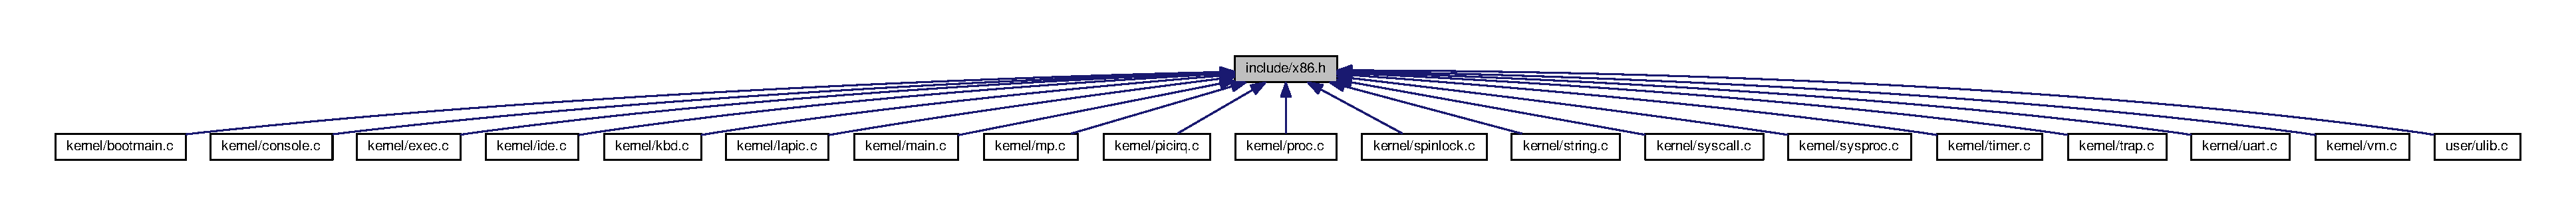
\includegraphics[width=350pt]{x86_8h__dep__incl}
\end{center}
\end{figure}
\subsection*{Data Structures}
\begin{DoxyCompactItemize}
\item 
struct \hyperlink{structtrapframe}{trapframe}
\end{DoxyCompactItemize}

\hypertarget{asm_8h}{\section{kernel/asm.h File Reference}
\label{asm_8h}\index{kernel/asm.\-h@{kernel/asm.\-h}}
}
\subsection*{Macros}
\begin{DoxyCompactItemize}
\item 
\#define \hyperlink{asm_8h_a0281b83dd2d5c19c39be963761f26e4f}{S\-E\-G\-\_\-\-N\-U\-L\-L\-A\-S\-M}
\item 
\#define \hyperlink{asm_8h_a56761ae3b4f4c70da4f433b9867e4e87}{S\-E\-G\-\_\-\-A\-S\-M}(type, base, lim)
\item 
\#define \hyperlink{asm_8h_af30c683a434e0712fd83781307239cb9}{S\-T\-A\-\_\-\-X}~0x8
\item 
\#define \hyperlink{asm_8h_ad6f4adbc6fea020a7d9d18a5f709843e}{S\-T\-A\-\_\-\-E}~0x4
\item 
\#define \hyperlink{asm_8h_ab4829c3150ed67ae0f00a103fb448a2f}{S\-T\-A\-\_\-\-C}~0x4
\item 
\#define \hyperlink{asm_8h_a9321b5b232838b8b230c6b681be9a882}{S\-T\-A\-\_\-\-W}~0x2
\item 
\#define \hyperlink{asm_8h_a6545a48f34a3fae1b04cf265f13bc8f3}{S\-T\-A\-\_\-\-R}~0x2
\item 
\#define \hyperlink{asm_8h_a18eb795a2eb72794f4de5b8087731607}{S\-T\-A\-\_\-\-A}~0x1
\end{DoxyCompactItemize}


\subsection{Macro Definition Documentation}
\hypertarget{asm_8h_a56761ae3b4f4c70da4f433b9867e4e87}{\index{asm.\-h@{asm.\-h}!S\-E\-G\-\_\-\-A\-S\-M@{S\-E\-G\-\_\-\-A\-S\-M}}
\index{S\-E\-G\-\_\-\-A\-S\-M@{S\-E\-G\-\_\-\-A\-S\-M}!asm.h@{asm.\-h}}
\subsubsection[{S\-E\-G\-\_\-\-A\-S\-M}]{\setlength{\rightskip}{0pt plus 5cm}\#define S\-E\-G\-\_\-\-A\-S\-M(
\begin{DoxyParamCaption}
\item[{}]{type, }
\item[{}]{base, }
\item[{}]{lim}
\end{DoxyParamCaption}
)}}\label{asm_8h_a56761ae3b4f4c70da4f433b9867e4e87}
{\bfseries Value\-:}
\begin{DoxyCode}
.word (((lim) >> 12) & 0xffff), ((base) & 0xffff);      \(\backslash\)
        .byte (((base) >> 16) & 0xff), (0x90 | (type)),         \(\backslash\)
                (0xC0 | (((lim) >> 28) & 0xf)), (((base) >> 24) & 0xff)
\end{DoxyCode}


Definition at line 11 of file asm.\-h.

\hypertarget{asm_8h_a0281b83dd2d5c19c39be963761f26e4f}{\index{asm.\-h@{asm.\-h}!S\-E\-G\-\_\-\-N\-U\-L\-L\-A\-S\-M@{S\-E\-G\-\_\-\-N\-U\-L\-L\-A\-S\-M}}
\index{S\-E\-G\-\_\-\-N\-U\-L\-L\-A\-S\-M@{S\-E\-G\-\_\-\-N\-U\-L\-L\-A\-S\-M}!asm.h@{asm.\-h}}
\subsubsection[{S\-E\-G\-\_\-\-N\-U\-L\-L\-A\-S\-M}]{\setlength{\rightskip}{0pt plus 5cm}\#define S\-E\-G\-\_\-\-N\-U\-L\-L\-A\-S\-M}}\label{asm_8h_a0281b83dd2d5c19c39be963761f26e4f}
{\bfseries Value\-:}
\begin{DoxyCode}
.word 0, 0;                                             \(\backslash\)
        .byte 0, 0, 0, 0
\end{DoxyCode}


Definition at line 5 of file asm.\-h.

\hypertarget{asm_8h_a18eb795a2eb72794f4de5b8087731607}{\index{asm.\-h@{asm.\-h}!S\-T\-A\-\_\-\-A@{S\-T\-A\-\_\-\-A}}
\index{S\-T\-A\-\_\-\-A@{S\-T\-A\-\_\-\-A}!asm.h@{asm.\-h}}
\subsubsection[{S\-T\-A\-\_\-\-A}]{\setlength{\rightskip}{0pt plus 5cm}\#define S\-T\-A\-\_\-\-A~0x1}}\label{asm_8h_a18eb795a2eb72794f4de5b8087731607}


Definition at line 21 of file asm.\-h.

\hypertarget{asm_8h_ab4829c3150ed67ae0f00a103fb448a2f}{\index{asm.\-h@{asm.\-h}!S\-T\-A\-\_\-\-C@{S\-T\-A\-\_\-\-C}}
\index{S\-T\-A\-\_\-\-C@{S\-T\-A\-\_\-\-C}!asm.h@{asm.\-h}}
\subsubsection[{S\-T\-A\-\_\-\-C}]{\setlength{\rightskip}{0pt plus 5cm}\#define S\-T\-A\-\_\-\-C~0x4}}\label{asm_8h_ab4829c3150ed67ae0f00a103fb448a2f}


Definition at line 18 of file asm.\-h.

\hypertarget{asm_8h_ad6f4adbc6fea020a7d9d18a5f709843e}{\index{asm.\-h@{asm.\-h}!S\-T\-A\-\_\-\-E@{S\-T\-A\-\_\-\-E}}
\index{S\-T\-A\-\_\-\-E@{S\-T\-A\-\_\-\-E}!asm.h@{asm.\-h}}
\subsubsection[{S\-T\-A\-\_\-\-E}]{\setlength{\rightskip}{0pt plus 5cm}\#define S\-T\-A\-\_\-\-E~0x4}}\label{asm_8h_ad6f4adbc6fea020a7d9d18a5f709843e}


Definition at line 17 of file asm.\-h.

\hypertarget{asm_8h_a6545a48f34a3fae1b04cf265f13bc8f3}{\index{asm.\-h@{asm.\-h}!S\-T\-A\-\_\-\-R@{S\-T\-A\-\_\-\-R}}
\index{S\-T\-A\-\_\-\-R@{S\-T\-A\-\_\-\-R}!asm.h@{asm.\-h}}
\subsubsection[{S\-T\-A\-\_\-\-R}]{\setlength{\rightskip}{0pt plus 5cm}\#define S\-T\-A\-\_\-\-R~0x2}}\label{asm_8h_a6545a48f34a3fae1b04cf265f13bc8f3}


Definition at line 20 of file asm.\-h.

\hypertarget{asm_8h_a9321b5b232838b8b230c6b681be9a882}{\index{asm.\-h@{asm.\-h}!S\-T\-A\-\_\-\-W@{S\-T\-A\-\_\-\-W}}
\index{S\-T\-A\-\_\-\-W@{S\-T\-A\-\_\-\-W}!asm.h@{asm.\-h}}
\subsubsection[{S\-T\-A\-\_\-\-W}]{\setlength{\rightskip}{0pt plus 5cm}\#define S\-T\-A\-\_\-\-W~0x2}}\label{asm_8h_a9321b5b232838b8b230c6b681be9a882}


Definition at line 19 of file asm.\-h.

\hypertarget{asm_8h_af30c683a434e0712fd83781307239cb9}{\index{asm.\-h@{asm.\-h}!S\-T\-A\-\_\-\-X@{S\-T\-A\-\_\-\-X}}
\index{S\-T\-A\-\_\-\-X@{S\-T\-A\-\_\-\-X}!asm.h@{asm.\-h}}
\subsubsection[{S\-T\-A\-\_\-\-X}]{\setlength{\rightskip}{0pt plus 5cm}\#define S\-T\-A\-\_\-\-X~0x8}}\label{asm_8h_af30c683a434e0712fd83781307239cb9}


Definition at line 16 of file asm.\-h.


\hypertarget{bio_8c}{\section{kernel/bio.c File Reference}
\label{bio_8c}\index{kernel/bio.\-c@{kernel/bio.\-c}}
}
{\ttfamily \#include \char`\"{}types.\-h\char`\"{}}\\*
{\ttfamily \#include \char`\"{}defs.\-h\char`\"{}}\\*
{\ttfamily \#include \char`\"{}param.\-h\char`\"{}}\\*
{\ttfamily \#include \char`\"{}spinlock.\-h\char`\"{}}\\*
{\ttfamily \#include \char`\"{}buf.\-h\char`\"{}}\\*
Include dependency graph for bio.\-c\-:
\nopagebreak
\begin{figure}[H]
\begin{center}
\leavevmode
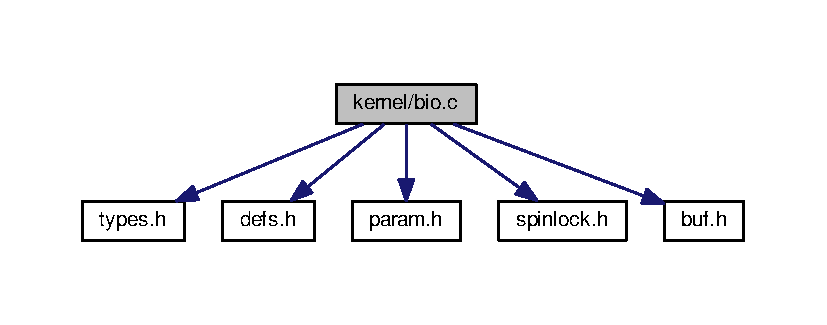
\includegraphics[width=350pt]{bio_8c__incl}
\end{center}
\end{figure}
\subsection*{Functions}
\begin{DoxyCompactItemize}
\item 
void \hyperlink{bio_8c_a53cca0ddc98c5f1de37124eca2575a59}{binit} (void)
\item 
struct \hyperlink{structbuf}{buf} $\ast$ \hyperlink{bio_8c_ac09898fdd6868e88ff35f498fa6ef52f}{bread} (\hyperlink{types_8h_a91ad9478d81a7aaf2593e8d9c3d06a14}{uint} dev, \hyperlink{types_8h_a91ad9478d81a7aaf2593e8d9c3d06a14}{uint} sector)
\item 
void \hyperlink{bio_8c_a63c899c13b176ddf80064d32225e1298}{bwrite} (struct \hyperlink{structbuf}{buf} $\ast$b)
\item 
void \hyperlink{bio_8c_ab5335aeb503731104314321a78a6d727}{brelse} (struct \hyperlink{structbuf}{buf} $\ast$b)
\end{DoxyCompactItemize}
\subsection*{Variables}
\begin{DoxyCompactItemize}
\item 
\begin{tabbing}
xx\=xx\=xx\=xx\=xx\=xx\=xx\=xx\=xx\=\kill
struct \{\\
\>struct \hyperlink{structspinlock}{spinlock} \hyperlink{bio_8c_ab28e82cd5dda7d960095706a3ea20572}{lock}\\
\>struct \hyperlink{structbuf}{buf} \hyperlink{bio_8c_a72ee90c61d41547b10a533c219e081c6}{buf} \mbox{[}\hyperlink{param_8h_ad51e2f8dffd163c263ec676a268d0f0a}{NBUF}\mbox{]}\\
\>struct \hyperlink{structbuf}{buf} \hyperlink{bio_8c_aa6e692c16f1b909f5cb2a1832cf43430}{head}\\
\} \hyperlink{bio_8c_a8c840c340a1233a78bdb2af607bbbcfc}{bcache}\\

\end{tabbing}\end{DoxyCompactItemize}


\subsection{Function Documentation}
\hypertarget{bio_8c_a53cca0ddc98c5f1de37124eca2575a59}{\index{bio.\-c@{bio.\-c}!binit@{binit}}
\index{binit@{binit}!bio.c@{bio.\-c}}
\subsubsection[{binit}]{\setlength{\rightskip}{0pt plus 5cm}void binit (
\begin{DoxyParamCaption}
\item[{void}]{}
\end{DoxyParamCaption}
)}}\label{bio_8c_a53cca0ddc98c5f1de37124eca2575a59}


Definition at line 40 of file bio.\-c.

\hypertarget{bio_8c_ac09898fdd6868e88ff35f498fa6ef52f}{\index{bio.\-c@{bio.\-c}!bread@{bread}}
\index{bread@{bread}!bio.c@{bio.\-c}}
\subsubsection[{bread}]{\setlength{\rightskip}{0pt plus 5cm}struct {\bf buf}$\ast$ bread (
\begin{DoxyParamCaption}
\item[{{\bf uint}}]{dev, }
\item[{{\bf uint}}]{sector}
\end{DoxyParamCaption}
)}}\label{bio_8c_ac09898fdd6868e88ff35f498fa6ef52f}


Definition at line 97 of file bio.\-c.

\hypertarget{bio_8c_ab5335aeb503731104314321a78a6d727}{\index{bio.\-c@{bio.\-c}!brelse@{brelse}}
\index{brelse@{brelse}!bio.c@{bio.\-c}}
\subsubsection[{brelse}]{\setlength{\rightskip}{0pt plus 5cm}void brelse (
\begin{DoxyParamCaption}
\item[{struct {\bf buf} $\ast$}]{b}
\end{DoxyParamCaption}
)}}\label{bio_8c_ab5335aeb503731104314321a78a6d727}


Definition at line 119 of file bio.\-c.

\hypertarget{bio_8c_a63c899c13b176ddf80064d32225e1298}{\index{bio.\-c@{bio.\-c}!bwrite@{bwrite}}
\index{bwrite@{bwrite}!bio.c@{bio.\-c}}
\subsubsection[{bwrite}]{\setlength{\rightskip}{0pt plus 5cm}void bwrite (
\begin{DoxyParamCaption}
\item[{struct {\bf buf} $\ast$}]{b}
\end{DoxyParamCaption}
)}}\label{bio_8c_a63c899c13b176ddf80064d32225e1298}


Definition at line 109 of file bio.\-c.



\subsection{Variable Documentation}
\hypertarget{bio_8c_a8c840c340a1233a78bdb2af607bbbcfc}{\index{bio.\-c@{bio.\-c}!bcache@{bcache}}
\index{bcache@{bcache}!bio.c@{bio.\-c}}
\subsubsection[{bcache}]{\setlength{\rightskip}{0pt plus 5cm}struct \{ ... \}   bcache}}\label{bio_8c_a8c840c340a1233a78bdb2af607bbbcfc}
\hypertarget{bio_8c_a72ee90c61d41547b10a533c219e081c6}{\index{bio.\-c@{bio.\-c}!buf@{buf}}
\index{buf@{buf}!bio.c@{bio.\-c}}
\subsubsection[{buf}]{\setlength{\rightskip}{0pt plus 5cm}struct {\bf buf} {\bf buf}\mbox{[}{\bf N\-B\-U\-F}\mbox{]}}}\label{bio_8c_a72ee90c61d41547b10a533c219e081c6}


Definition at line 32 of file bio.\-c.

\hypertarget{bio_8c_aa6e692c16f1b909f5cb2a1832cf43430}{\index{bio.\-c@{bio.\-c}!head@{head}}
\index{head@{head}!bio.c@{bio.\-c}}
\subsubsection[{head}]{\setlength{\rightskip}{0pt plus 5cm}struct {\bf buf} head}}\label{bio_8c_aa6e692c16f1b909f5cb2a1832cf43430}


Definition at line 36 of file bio.\-c.

\hypertarget{bio_8c_ab28e82cd5dda7d960095706a3ea20572}{\index{bio.\-c@{bio.\-c}!lock@{lock}}
\index{lock@{lock}!bio.c@{bio.\-c}}
\subsubsection[{lock}]{\setlength{\rightskip}{0pt plus 5cm}struct {\bf spinlock} lock}}\label{bio_8c_ab28e82cd5dda7d960095706a3ea20572}


Definition at line 31 of file bio.\-c.


\hypertarget{bio_8d}{\section{kernel/bio.d File Reference}
\label{bio_8d}\index{kernel/bio.\-d@{kernel/bio.\-d}}
}

\hypertarget{bootasm_8d}{\section{kernel/bootasm.d File Reference}
\label{bootasm_8d}\index{kernel/bootasm.\-d@{kernel/bootasm.\-d}}
}

\hypertarget{bootmain_8c}{\section{kernel/bootmain.c File Reference}
\label{bootmain_8c}\index{kernel/bootmain.\-c@{kernel/bootmain.\-c}}
}
{\ttfamily \#include \char`\"{}types.\-h\char`\"{}}\\*
{\ttfamily \#include \char`\"{}elf.\-h\char`\"{}}\\*
{\ttfamily \#include \char`\"{}x86.\-h\char`\"{}}\\*
Include dependency graph for bootmain.\-c\-:
\nopagebreak
\begin{figure}[H]
\begin{center}
\leavevmode
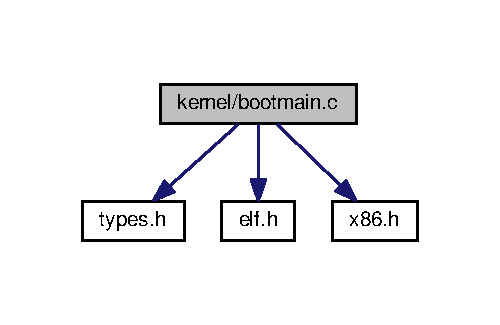
\includegraphics[width=240pt]{bootmain_8c__incl}
\end{center}
\end{figure}
\subsection*{Macros}
\begin{DoxyCompactItemize}
\item 
\#define \hyperlink{bootmain_8c_af69dd8b281718a66b3e7a65250d24419}{S\-E\-C\-T\-S\-I\-Z\-E}~512
\end{DoxyCompactItemize}
\subsection*{Functions}
\begin{DoxyCompactItemize}
\item 
void \hyperlink{bootmain_8c_af8097ce47ae21ccad1b0afd6f48ef62c}{readseg} (\hyperlink{types_8h_a65f85814a8290f9797005d3b28e7e5fc}{uchar} $\ast$, \hyperlink{types_8h_a91ad9478d81a7aaf2593e8d9c3d06a14}{uint}, \hyperlink{types_8h_a91ad9478d81a7aaf2593e8d9c3d06a14}{uint})
\item 
void \hyperlink{bootmain_8c_a0d198d492591e1b70a8a12109408a7e4}{bootmain} (void)
\item 
void \hyperlink{bootmain_8c_a63222d4a07c38c198de5bd116a001935}{waitdisk} (void)
\item 
void \hyperlink{bootmain_8c_ae7ef59ffa082283b72c54e43b7a16351}{readsect} (void $\ast$dst, \hyperlink{types_8h_a91ad9478d81a7aaf2593e8d9c3d06a14}{uint} offset)
\end{DoxyCompactItemize}


\subsection{Macro Definition Documentation}
\hypertarget{bootmain_8c_af69dd8b281718a66b3e7a65250d24419}{\index{bootmain.\-c@{bootmain.\-c}!S\-E\-C\-T\-S\-I\-Z\-E@{S\-E\-C\-T\-S\-I\-Z\-E}}
\index{S\-E\-C\-T\-S\-I\-Z\-E@{S\-E\-C\-T\-S\-I\-Z\-E}!bootmain.c@{bootmain.\-c}}
\subsubsection[{S\-E\-C\-T\-S\-I\-Z\-E}]{\setlength{\rightskip}{0pt plus 5cm}\#define S\-E\-C\-T\-S\-I\-Z\-E~512}}\label{bootmain_8c_af69dd8b281718a66b3e7a65250d24419}


Definition at line 12 of file bootmain.\-c.



\subsection{Function Documentation}
\hypertarget{bootmain_8c_a0d198d492591e1b70a8a12109408a7e4}{\index{bootmain.\-c@{bootmain.\-c}!bootmain@{bootmain}}
\index{bootmain@{bootmain}!bootmain.c@{bootmain.\-c}}
\subsubsection[{bootmain}]{\setlength{\rightskip}{0pt plus 5cm}void bootmain (
\begin{DoxyParamCaption}
\item[{void}]{}
\end{DoxyParamCaption}
)}}\label{bootmain_8c_a0d198d492591e1b70a8a12109408a7e4}


Definition at line 17 of file bootmain.\-c.

\hypertarget{bootmain_8c_ae7ef59ffa082283b72c54e43b7a16351}{\index{bootmain.\-c@{bootmain.\-c}!readsect@{readsect}}
\index{readsect@{readsect}!bootmain.c@{bootmain.\-c}}
\subsubsection[{readsect}]{\setlength{\rightskip}{0pt plus 5cm}void readsect (
\begin{DoxyParamCaption}
\item[{void $\ast$}]{dst, }
\item[{{\bf uint}}]{offset}
\end{DoxyParamCaption}
)}}\label{bootmain_8c_ae7ef59ffa082283b72c54e43b7a16351}


Definition at line 59 of file bootmain.\-c.

\hypertarget{bootmain_8c_af8097ce47ae21ccad1b0afd6f48ef62c}{\index{bootmain.\-c@{bootmain.\-c}!readseg@{readseg}}
\index{readseg@{readseg}!bootmain.c@{bootmain.\-c}}
\subsubsection[{readseg}]{\setlength{\rightskip}{0pt plus 5cm}void readseg (
\begin{DoxyParamCaption}
\item[{{\bf uchar} $\ast$}]{va, }
\item[{{\bf uint}}]{count, }
\item[{{\bf uint}}]{offset}
\end{DoxyParamCaption}
)}}\label{bootmain_8c_af8097ce47ae21ccad1b0afd6f48ef62c}


Definition at line 78 of file bootmain.\-c.

\hypertarget{bootmain_8c_a63222d4a07c38c198de5bd116a001935}{\index{bootmain.\-c@{bootmain.\-c}!waitdisk@{waitdisk}}
\index{waitdisk@{waitdisk}!bootmain.c@{bootmain.\-c}}
\subsubsection[{waitdisk}]{\setlength{\rightskip}{0pt plus 5cm}void waitdisk (
\begin{DoxyParamCaption}
\item[{void}]{}
\end{DoxyParamCaption}
)}}\label{bootmain_8c_a63222d4a07c38c198de5bd116a001935}


Definition at line 50 of file bootmain.\-c.


\hypertarget{bootmain_8d}{\section{kernel/bootmain.d File Reference}
\label{bootmain_8d}\index{kernel/bootmain.\-d@{kernel/bootmain.\-d}}
}

\hypertarget{bootother_8d}{\section{kernel/bootother.d File Reference}
\label{bootother_8d}\index{kernel/bootother.\-d@{kernel/bootother.\-d}}
}

\hypertarget{buf_8h}{\section{kernel/buf.h File Reference}
\label{buf_8h}\index{kernel/buf.\-h@{kernel/buf.\-h}}
}
This graph shows which files directly or indirectly include this file\-:
\nopagebreak
\begin{figure}[H]
\begin{center}
\leavevmode
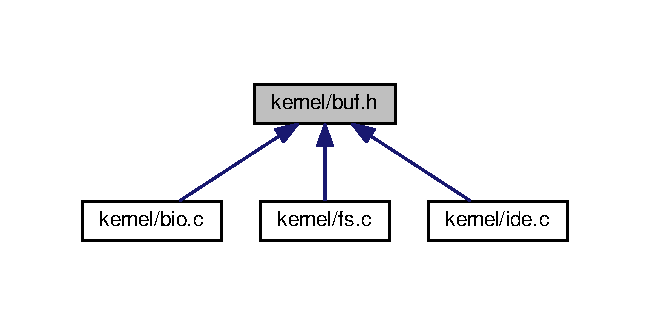
\includegraphics[width=312pt]{buf_8h__dep__incl}
\end{center}
\end{figure}
\subsection*{Data Structures}
\begin{DoxyCompactItemize}
\item 
struct \hyperlink{structbuf}{buf}
\end{DoxyCompactItemize}
\subsection*{Macros}
\begin{DoxyCompactItemize}
\item 
\#define \hyperlink{buf_8h_abd2b4f84a360399fba6535a0d5f33298}{B\-\_\-\-B\-U\-S\-Y}~0x1
\item 
\#define \hyperlink{buf_8h_afab4199c0d27da71061f1c0cd5b51520}{B\-\_\-\-V\-A\-L\-I\-D}~0x2
\item 
\#define \hyperlink{buf_8h_adc32011df267adb9740bcd0abf0f0663}{B\-\_\-\-D\-I\-R\-T\-Y}~0x4
\end{DoxyCompactItemize}


\subsection{Macro Definition Documentation}
\hypertarget{buf_8h_abd2b4f84a360399fba6535a0d5f33298}{\index{buf.\-h@{buf.\-h}!B\-\_\-\-B\-U\-S\-Y@{B\-\_\-\-B\-U\-S\-Y}}
\index{B\-\_\-\-B\-U\-S\-Y@{B\-\_\-\-B\-U\-S\-Y}!buf.h@{buf.\-h}}
\subsubsection[{B\-\_\-\-B\-U\-S\-Y}]{\setlength{\rightskip}{0pt plus 5cm}\#define B\-\_\-\-B\-U\-S\-Y~0x1}}\label{buf_8h_abd2b4f84a360399fba6535a0d5f33298}


Definition at line 13 of file buf.\-h.

\hypertarget{buf_8h_adc32011df267adb9740bcd0abf0f0663}{\index{buf.\-h@{buf.\-h}!B\-\_\-\-D\-I\-R\-T\-Y@{B\-\_\-\-D\-I\-R\-T\-Y}}
\index{B\-\_\-\-D\-I\-R\-T\-Y@{B\-\_\-\-D\-I\-R\-T\-Y}!buf.h@{buf.\-h}}
\subsubsection[{B\-\_\-\-D\-I\-R\-T\-Y}]{\setlength{\rightskip}{0pt plus 5cm}\#define B\-\_\-\-D\-I\-R\-T\-Y~0x4}}\label{buf_8h_adc32011df267adb9740bcd0abf0f0663}


Definition at line 15 of file buf.\-h.

\hypertarget{buf_8h_afab4199c0d27da71061f1c0cd5b51520}{\index{buf.\-h@{buf.\-h}!B\-\_\-\-V\-A\-L\-I\-D@{B\-\_\-\-V\-A\-L\-I\-D}}
\index{B\-\_\-\-V\-A\-L\-I\-D@{B\-\_\-\-V\-A\-L\-I\-D}!buf.h@{buf.\-h}}
\subsubsection[{B\-\_\-\-V\-A\-L\-I\-D}]{\setlength{\rightskip}{0pt plus 5cm}\#define B\-\_\-\-V\-A\-L\-I\-D~0x2}}\label{buf_8h_afab4199c0d27da71061f1c0cd5b51520}


Definition at line 14 of file buf.\-h.


\hypertarget{console_8c}{\section{kernel/console.c File Reference}
\label{console_8c}\index{kernel/console.\-c@{kernel/console.\-c}}
}
{\ttfamily \#include \char`\"{}types.\-h\char`\"{}}\\*
{\ttfamily \#include \char`\"{}defs.\-h\char`\"{}}\\*
{\ttfamily \#include \char`\"{}param.\-h\char`\"{}}\\*
{\ttfamily \#include \char`\"{}traps.\-h\char`\"{}}\\*
{\ttfamily \#include \char`\"{}spinlock.\-h\char`\"{}}\\*
{\ttfamily \#include \char`\"{}fs.\-h\char`\"{}}\\*
{\ttfamily \#include \char`\"{}file.\-h\char`\"{}}\\*
{\ttfamily \#include \char`\"{}mmu.\-h\char`\"{}}\\*
{\ttfamily \#include \char`\"{}proc.\-h\char`\"{}}\\*
{\ttfamily \#include \char`\"{}x86.\-h\char`\"{}}\\*
Include dependency graph for console.\-c\-:
\nopagebreak
\begin{figure}[H]
\begin{center}
\leavevmode
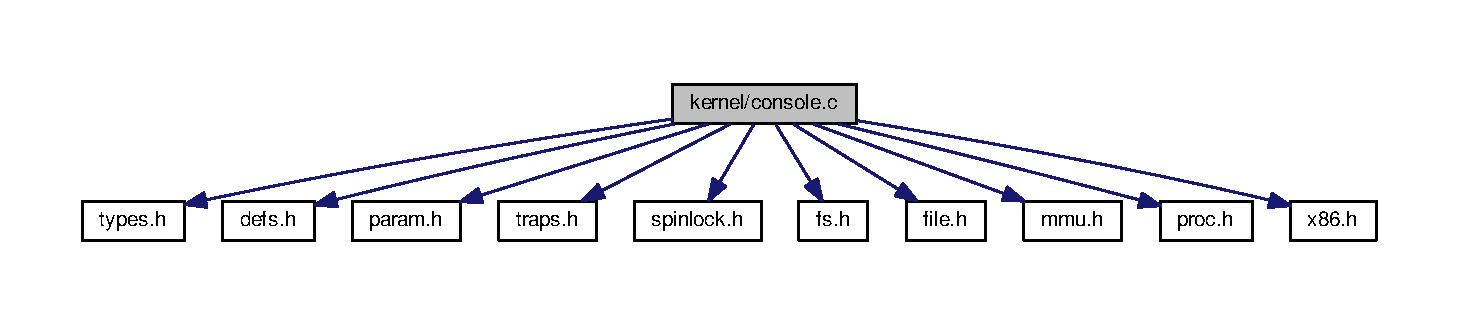
\includegraphics[width=350pt]{console_8c__incl}
\end{center}
\end{figure}
\subsection*{Macros}
\begin{DoxyCompactItemize}
\item 
\#define \hyperlink{console_8c_a629568514359445d2fbda71d70eeb1ce}{B\-A\-C\-K\-S\-P\-A\-C\-E}~0x100
\item 
\#define \hyperlink{console_8c_a2e3959df0a0c54f50f20d4776b14487f}{C\-R\-T\-P\-O\-R\-T}~0x3d4
\item 
\#define \hyperlink{console_8c_a5d85434f2a29f6c3048aeac34d0ce41d}{I\-N\-P\-U\-T\-\_\-\-B\-U\-F}~128
\item 
\#define \hyperlink{console_8c_ac54ae397901fe700628cafadea3c5208}{C}(x)~((x)-\/'@')
\end{DoxyCompactItemize}
\subsection*{Functions}
\begin{DoxyCompactItemize}
\item 
void \hyperlink{console_8c_a90f0742d846503e4ed1804f1df421ec6}{cprintf} (char $\ast$fmt,...)
\item 
void \hyperlink{console_8c_a95c0aca5d6d7487933984f08b189917a}{panic} (char $\ast$s)
\item 
void \hyperlink{console_8c_aad3d6ca39f23bb6d2686d2967e415193}{consoleintr} (int($\ast$getc)(void))
\item 
int \hyperlink{console_8c_a28ac85a90987662e306ca8efbfe16074}{consoleread} (struct \hyperlink{structinode}{inode} $\ast$ip, char $\ast$dst, int n)
\item 
int \hyperlink{console_8c_a6af7eb39268127d389792cec37785666}{consolewrite} (struct \hyperlink{structinode}{inode} $\ast$ip, char $\ast$\hyperlink{structbuf}{buf}, int n)
\item 
void \hyperlink{console_8c_ab508ff0f4db26fe35cd25fa648f9ee75}{consoleinit} (void)
\end{DoxyCompactItemize}
\subsection*{Variables}
\begin{DoxyCompactItemize}
\item 
\begin{tabbing}
xx\=xx\=xx\=xx\=xx\=xx\=xx\=xx\=xx\=\kill
struct \{\\
\>struct \hyperlink{structspinlock}{spinlock} \hyperlink{console_8c_ab28e82cd5dda7d960095706a3ea20572}{lock}\\
\>char \hyperlink{console_8c_aa427837782b05b05204809dfba33c8f5}{buf} \mbox{[}\hyperlink{console_8c_a5d85434f2a29f6c3048aeac34d0ce41d}{INPUT\_BUF}\mbox{]}\\
\>\hyperlink{types_8h_a91ad9478d81a7aaf2593e8d9c3d06a14}{uint} \hyperlink{console_8c_af10fa12dd785c91e29528fbdc50cf9af}{r}\\
\>\hyperlink{types_8h_a91ad9478d81a7aaf2593e8d9c3d06a14}{uint} \hyperlink{console_8c_afdeff54db9a334718662b709641fdfe1}{w}\\
\>\hyperlink{types_8h_a91ad9478d81a7aaf2593e8d9c3d06a14}{uint} \hyperlink{console_8c_ab56fa7c992b725d84916b987c3d532ea}{e}\\
\} \hyperlink{console_8c_a41db130acd332cdb95756628cfb2e48b}{input}\\

\end{tabbing}\end{DoxyCompactItemize}


\subsection{Macro Definition Documentation}
\hypertarget{console_8c_a629568514359445d2fbda71d70eeb1ce}{\index{console.\-c@{console.\-c}!B\-A\-C\-K\-S\-P\-A\-C\-E@{B\-A\-C\-K\-S\-P\-A\-C\-E}}
\index{B\-A\-C\-K\-S\-P\-A\-C\-E@{B\-A\-C\-K\-S\-P\-A\-C\-E}!console.c@{console.\-c}}
\subsubsection[{B\-A\-C\-K\-S\-P\-A\-C\-E}]{\setlength{\rightskip}{0pt plus 5cm}\#define B\-A\-C\-K\-S\-P\-A\-C\-E~0x100}}\label{console_8c_a629568514359445d2fbda71d70eeb1ce}


Definition at line 119 of file console.\-c.

\hypertarget{console_8c_ac54ae397901fe700628cafadea3c5208}{\index{console.\-c@{console.\-c}!C@{C}}
\index{C@{C}!console.c@{console.\-c}}
\subsubsection[{C}]{\setlength{\rightskip}{0pt plus 5cm}\#define C(
\begin{DoxyParamCaption}
\item[{}]{x}
\end{DoxyParamCaption}
)~((x)-\/'@')}}\label{console_8c_ac54ae397901fe700628cafadea3c5208}


Definition at line 179 of file console.\-c.

\hypertarget{console_8c_a2e3959df0a0c54f50f20d4776b14487f}{\index{console.\-c@{console.\-c}!C\-R\-T\-P\-O\-R\-T@{C\-R\-T\-P\-O\-R\-T}}
\index{C\-R\-T\-P\-O\-R\-T@{C\-R\-T\-P\-O\-R\-T}!console.c@{console.\-c}}
\subsubsection[{C\-R\-T\-P\-O\-R\-T}]{\setlength{\rightskip}{0pt plus 5cm}\#define C\-R\-T\-P\-O\-R\-T~0x3d4}}\label{console_8c_a2e3959df0a0c54f50f20d4776b14487f}


Definition at line 120 of file console.\-c.

\hypertarget{console_8c_a5d85434f2a29f6c3048aeac34d0ce41d}{\index{console.\-c@{console.\-c}!I\-N\-P\-U\-T\-\_\-\-B\-U\-F@{I\-N\-P\-U\-T\-\_\-\-B\-U\-F}}
\index{I\-N\-P\-U\-T\-\_\-\-B\-U\-F@{I\-N\-P\-U\-T\-\_\-\-B\-U\-F}!console.c@{console.\-c}}
\subsubsection[{I\-N\-P\-U\-T\-\_\-\-B\-U\-F}]{\setlength{\rightskip}{0pt plus 5cm}\#define I\-N\-P\-U\-T\-\_\-\-B\-U\-F~128}}\label{console_8c_a5d85434f2a29f6c3048aeac34d0ce41d}


Definition at line 170 of file console.\-c.



\subsection{Function Documentation}
\hypertarget{console_8c_ab508ff0f4db26fe35cd25fa648f9ee75}{\index{console.\-c@{console.\-c}!consoleinit@{consoleinit}}
\index{consoleinit@{consoleinit}!console.c@{console.\-c}}
\subsubsection[{consoleinit}]{\setlength{\rightskip}{0pt plus 5cm}void consoleinit (
\begin{DoxyParamCaption}
\item[{void}]{}
\end{DoxyParamCaption}
)}}\label{console_8c_ab508ff0f4db26fe35cd25fa648f9ee75}


Definition at line 275 of file console.\-c.

\hypertarget{console_8c_aad3d6ca39f23bb6d2686d2967e415193}{\index{console.\-c@{console.\-c}!consoleintr@{consoleintr}}
\index{consoleintr@{consoleintr}!console.c@{console.\-c}}
\subsubsection[{consoleintr}]{\setlength{\rightskip}{0pt plus 5cm}void consoleintr (
\begin{DoxyParamCaption}
\item[{int($\ast$)(void)}]{getc}
\end{DoxyParamCaption}
)}}\label{console_8c_aad3d6ca39f23bb6d2686d2967e415193}


Definition at line 182 of file console.\-c.

\hypertarget{console_8c_a28ac85a90987662e306ca8efbfe16074}{\index{console.\-c@{console.\-c}!consoleread@{consoleread}}
\index{consoleread@{consoleread}!console.c@{console.\-c}}
\subsubsection[{consoleread}]{\setlength{\rightskip}{0pt plus 5cm}int consoleread (
\begin{DoxyParamCaption}
\item[{struct {\bf inode} $\ast$}]{ip, }
\item[{char $\ast$}]{dst, }
\item[{int}]{n}
\end{DoxyParamCaption}
)}}\label{console_8c_a28ac85a90987662e306ca8efbfe16074}


Definition at line 222 of file console.\-c.

\hypertarget{console_8c_a6af7eb39268127d389792cec37785666}{\index{console.\-c@{console.\-c}!consolewrite@{consolewrite}}
\index{consolewrite@{consolewrite}!console.c@{console.\-c}}
\subsubsection[{consolewrite}]{\setlength{\rightskip}{0pt plus 5cm}int consolewrite (
\begin{DoxyParamCaption}
\item[{struct {\bf inode} $\ast$}]{ip, }
\item[{char $\ast$}]{buf, }
\item[{int}]{n}
\end{DoxyParamCaption}
)}}\label{console_8c_a6af7eb39268127d389792cec37785666}


Definition at line 260 of file console.\-c.

\hypertarget{console_8c_a90f0742d846503e4ed1804f1df421ec6}{\index{console.\-c@{console.\-c}!cprintf@{cprintf}}
\index{cprintf@{cprintf}!console.c@{console.\-c}}
\subsubsection[{cprintf}]{\setlength{\rightskip}{0pt plus 5cm}void cprintf (
\begin{DoxyParamCaption}
\item[{char $\ast$}]{fmt, }
\item[{}]{...}
\end{DoxyParamCaption}
)}}\label{console_8c_a90f0742d846503e4ed1804f1df421ec6}


Definition at line 52 of file console.\-c.

\hypertarget{console_8c_a95c0aca5d6d7487933984f08b189917a}{\index{console.\-c@{console.\-c}!panic@{panic}}
\index{panic@{panic}!console.c@{console.\-c}}
\subsubsection[{panic}]{\setlength{\rightskip}{0pt plus 5cm}void panic (
\begin{DoxyParamCaption}
\item[{char $\ast$}]{s}
\end{DoxyParamCaption}
)}}\label{console_8c_a95c0aca5d6d7487933984f08b189917a}


Definition at line 101 of file console.\-c.



\subsection{Variable Documentation}
\hypertarget{console_8c_aa427837782b05b05204809dfba33c8f5}{\index{console.\-c@{console.\-c}!buf@{buf}}
\index{buf@{buf}!console.c@{console.\-c}}
\subsubsection[{buf}]{\setlength{\rightskip}{0pt plus 5cm}char {\bf buf}\mbox{[}{\bf I\-N\-P\-U\-T\-\_\-\-B\-U\-F}\mbox{]}}}\label{console_8c_aa427837782b05b05204809dfba33c8f5}


Definition at line 173 of file console.\-c.

\hypertarget{console_8c_ab56fa7c992b725d84916b987c3d532ea}{\index{console.\-c@{console.\-c}!e@{e}}
\index{e@{e}!console.c@{console.\-c}}
\subsubsection[{e}]{\setlength{\rightskip}{0pt plus 5cm}{\bf uint} e}}\label{console_8c_ab56fa7c992b725d84916b987c3d532ea}


Definition at line 176 of file console.\-c.

\hypertarget{console_8c_a41db130acd332cdb95756628cfb2e48b}{\index{console.\-c@{console.\-c}!input@{input}}
\index{input@{input}!console.c@{console.\-c}}
\subsubsection[{input}]{\setlength{\rightskip}{0pt plus 5cm}struct \{ ... \}   input}}\label{console_8c_a41db130acd332cdb95756628cfb2e48b}
\hypertarget{console_8c_ab28e82cd5dda7d960095706a3ea20572}{\index{console.\-c@{console.\-c}!lock@{lock}}
\index{lock@{lock}!console.c@{console.\-c}}
\subsubsection[{lock}]{\setlength{\rightskip}{0pt plus 5cm}struct {\bf spinlock} lock}}\label{console_8c_ab28e82cd5dda7d960095706a3ea20572}


Definition at line 21 of file console.\-c.

\hypertarget{console_8c_ae51110da3bc13ef49e32d1e2cda5d55c}{\index{console.\-c@{console.\-c}!locking@{locking}}
\index{locking@{locking}!console.c@{console.\-c}}
\subsubsection[{locking}]{\setlength{\rightskip}{0pt plus 5cm}int locking}}\label{console_8c_ae51110da3bc13ef49e32d1e2cda5d55c}


Definition at line 22 of file console.\-c.

\hypertarget{console_8c_af10fa12dd785c91e29528fbdc50cf9af}{\index{console.\-c@{console.\-c}!r@{r}}
\index{r@{r}!console.c@{console.\-c}}
\subsubsection[{r}]{\setlength{\rightskip}{0pt plus 5cm}{\bf uint} r}}\label{console_8c_af10fa12dd785c91e29528fbdc50cf9af}


Definition at line 174 of file console.\-c.

\hypertarget{console_8c_afdeff54db9a334718662b709641fdfe1}{\index{console.\-c@{console.\-c}!w@{w}}
\index{w@{w}!console.c@{console.\-c}}
\subsubsection[{w}]{\setlength{\rightskip}{0pt plus 5cm}{\bf uint} w}}\label{console_8c_afdeff54db9a334718662b709641fdfe1}


Definition at line 175 of file console.\-c.


\hypertarget{console_8d}{\section{kernel/console.d File Reference}
\label{console_8d}\index{kernel/console.\-d@{kernel/console.\-d}}
}

\hypertarget{data_8d}{\section{kernel/data.d File Reference}
\label{data_8d}\index{kernel/data.\-d@{kernel/data.\-d}}
}

\hypertarget{defs_8h}{\section{kernel/defs.h File Reference}
\label{defs_8h}\index{kernel/defs.\-h@{kernel/defs.\-h}}
}
This graph shows which files directly or indirectly include this file\-:
\nopagebreak
\begin{figure}[H]
\begin{center}
\leavevmode
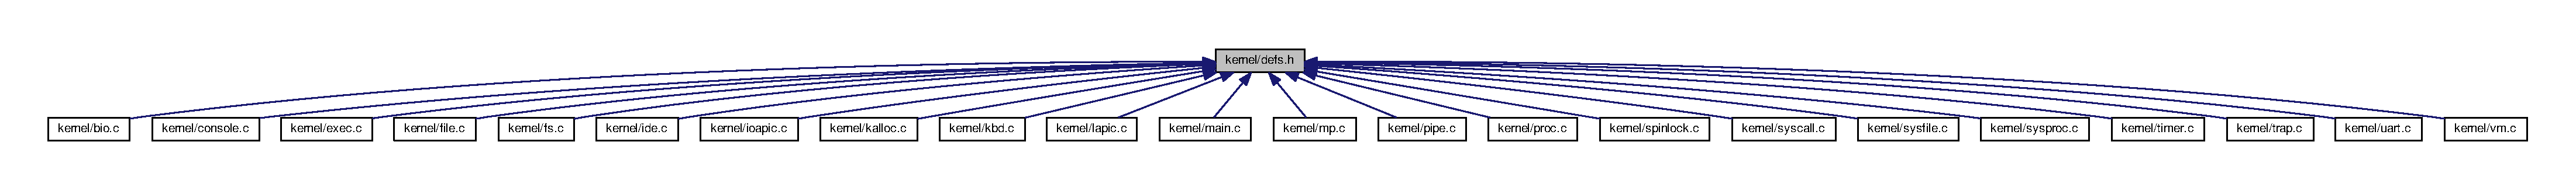
\includegraphics[width=350pt]{defs_8h__dep__incl}
\end{center}
\end{figure}
\subsection*{Macros}
\begin{DoxyCompactItemize}
\item 
\#define \hyperlink{defs_8h_afacd331296c10f360da7640e0d68429f}{N\-E\-L\-E\-M}(x)~(sizeof(x)/sizeof((x)\mbox{[}0\mbox{]}))
\end{DoxyCompactItemize}
\subsection*{Functions}
\begin{DoxyCompactItemize}
\item 
void \hyperlink{defs_8h_a53cca0ddc98c5f1de37124eca2575a59}{binit} (void)
\item 
struct \hyperlink{structbuf}{buf} $\ast$ \hyperlink{defs_8h_a90c72cf2140fdf1612484117327220af}{bread} (\hyperlink{types_8h_a91ad9478d81a7aaf2593e8d9c3d06a14}{uint}, \hyperlink{types_8h_a91ad9478d81a7aaf2593e8d9c3d06a14}{uint})
\item 
void \hyperlink{defs_8h_aa31ec2f79e0456737a9680270bc1841b}{brelse} (struct \hyperlink{structbuf}{buf} $\ast$)
\item 
void \hyperlink{defs_8h_a1bfd775f14ad3dfee354ee3897ecd28d}{bwrite} (struct \hyperlink{structbuf}{buf} $\ast$)
\item 
void \hyperlink{defs_8h_ab508ff0f4db26fe35cd25fa648f9ee75}{consoleinit} (void)
\item 
void \hyperlink{defs_8h_abeb2bc020e7332bcde1d7beab08582d3}{cprintf} (char $\ast$,...)
\item 
void \hyperlink{defs_8h_a9ec968a6fc407075634fe0e82a9c6862}{consoleintr} (int($\ast$)(void))
\item 
void \hyperlink{defs_8h_a45323e3f295a0d9b90929cc30a24e2aa}{panic} (char $\ast$) \-\_\-\-\_\-attribute\-\_\-\-\_\-((noreturn))
\item 
int \hyperlink{defs_8h_aa7b4aae4a12acd187e23396214aeca47}{exec} (char $\ast$, char $\ast$$\ast$)
\item 
struct \hyperlink{structfile}{file} $\ast$ \hyperlink{defs_8h_a69d3d2dd94efa1f1ff8d0143f4d9b786}{filealloc} (void)
\item 
void \hyperlink{defs_8h_ac865ee0b2d70f753d61d1fefef9de0f6}{fileclose} (struct \hyperlink{structfile}{file} $\ast$)
\item 
struct \hyperlink{structfile}{file} $\ast$ \hyperlink{defs_8h_a1063546fe0d5f45fe1a38a9b4f6b5783}{filedup} (struct \hyperlink{structfile}{file} $\ast$)
\item 
void \hyperlink{defs_8h_a66bb5a4b304ea0f851dd999fc8195fa4}{fileinit} (void)
\item 
int \hyperlink{defs_8h_a6bd1db179155944c9d1fbc89d8b7b162}{fileread} (struct \hyperlink{structfile}{file} $\ast$, char $\ast$, int n)
\item 
int \hyperlink{defs_8h_ac4979f97957194db01001985b1bfa84e}{filestat} (struct \hyperlink{structfile}{file} $\ast$, struct \hyperlink{structstat}{stat} $\ast$)
\item 
int \hyperlink{defs_8h_a90e8980df48fa900fc33de53448a2e18}{filewrite} (struct \hyperlink{structfile}{file} $\ast$, char $\ast$, int n)
\item 
int \hyperlink{defs_8h_ae4ccea0aa02557162963e597737f665a}{dirlink} (struct \hyperlink{structinode}{inode} $\ast$, char $\ast$, \hyperlink{types_8h_a91ad9478d81a7aaf2593e8d9c3d06a14}{uint})
\item 
struct \hyperlink{structinode}{inode} $\ast$ \hyperlink{defs_8h_a91ded9e61402d5e0d9f16b2a8cbff5c3}{dirlookup} (struct \hyperlink{structinode}{inode} $\ast$, char $\ast$, \hyperlink{types_8h_a91ad9478d81a7aaf2593e8d9c3d06a14}{uint} $\ast$)
\item 
struct \hyperlink{structinode}{inode} $\ast$ \hyperlink{defs_8h_ab4d7f391ca5219199e1b7502ac12ea85}{ialloc} (\hyperlink{types_8h_a91ad9478d81a7aaf2593e8d9c3d06a14}{uint}, short)
\item 
struct \hyperlink{structinode}{inode} $\ast$ \hyperlink{defs_8h_acdd1de79a331b8922c483434d257731d}{idup} (struct \hyperlink{structinode}{inode} $\ast$)
\item 
void \hyperlink{defs_8h_a508e2b44186d5b3997a1564fe5a6c2d9}{iinit} (void)
\item 
void \hyperlink{defs_8h_a29a4d743d41fe659f74b0a57fdc25012}{ilock} (struct \hyperlink{structinode}{inode} $\ast$)
\item 
void \hyperlink{defs_8h_a29530a0afdfe924818d8c70b6724528d}{iput} (struct \hyperlink{structinode}{inode} $\ast$)
\item 
void \hyperlink{defs_8h_af301c10ad8ced77a5dfb2de3a64c666c}{iunlock} (struct \hyperlink{structinode}{inode} $\ast$)
\item 
void \hyperlink{defs_8h_adff5bb5a1eeaf921853ec06479f8c49b}{iunlockput} (struct \hyperlink{structinode}{inode} $\ast$)
\item 
void \hyperlink{defs_8h_a2ee6784c123b2a2656d88b5b357f2253}{iupdate} (struct \hyperlink{structinode}{inode} $\ast$)
\item 
int \hyperlink{defs_8h_a0206c4090dc4bdfd8481e38057d5b2af}{namecmp} (const char $\ast$, const char $\ast$)
\item 
struct \hyperlink{structinode}{inode} $\ast$ \hyperlink{defs_8h_a29aa723e0b59f069c9eba588fdeb7e5a}{namei} (char $\ast$)
\item 
struct \hyperlink{structinode}{inode} $\ast$ \hyperlink{defs_8h_a02a47e8fb060db0a29727f29879024cc}{nameiparent} (char $\ast$, char $\ast$)
\item 
int \hyperlink{defs_8h_a2415273b06f31f0f2587b7325588a7e4}{readi} (struct \hyperlink{structinode}{inode} $\ast$, char $\ast$, \hyperlink{types_8h_a91ad9478d81a7aaf2593e8d9c3d06a14}{uint}, \hyperlink{types_8h_a91ad9478d81a7aaf2593e8d9c3d06a14}{uint})
\item 
void \hyperlink{defs_8h_a528f45ea5530504abc7113acc2154348}{stati} (struct \hyperlink{structinode}{inode} $\ast$, struct \hyperlink{structstat}{stat} $\ast$)
\item 
int \hyperlink{defs_8h_a515876d4653cefef4732806ef7f2833f}{writei} (struct \hyperlink{structinode}{inode} $\ast$, char $\ast$, \hyperlink{types_8h_a91ad9478d81a7aaf2593e8d9c3d06a14}{uint}, \hyperlink{types_8h_a91ad9478d81a7aaf2593e8d9c3d06a14}{uint})
\item 
void \hyperlink{defs_8h_aefb190a6104cb58c0bc1f8fec88d1307}{ideinit} (void)
\item 
void \hyperlink{defs_8h_a709693afdb9b89d848e684e7acde1f8f}{ideintr} (void)
\item 
void \hyperlink{defs_8h_a70985c3f5b2fb79737457b5c88f5327a}{iderw} (struct \hyperlink{structbuf}{buf} $\ast$)
\item 
void \hyperlink{defs_8h_a63da75c0c2f0b051f2c790aea2116b63}{ioapicenable} (int irq, int \hyperlink{structcpu}{cpu})
\item 
void \hyperlink{defs_8h_abce023b98422f397abdb425b20c8ceec}{ioapicinit} (void)
\item 
char $\ast$ \hyperlink{defs_8h_a3af104ba40b66dcec8363ac5a70907ed}{kalloc} (void)
\item 
void \hyperlink{defs_8h_ae79d6a7d0901b7c081cfded3f916d5bd}{kfree} (char $\ast$)
\item 
void \hyperlink{defs_8h_a71d803d14f0e1b0682e2c20e7c2a7f7a}{kinit} (void)
\item 
void \hyperlink{defs_8h_af3d6113fa152781400e1e0e728c55e54}{kbdintr} (void)
\item 
int \hyperlink{defs_8h_ad07bc98847d46ba9772ab5ad4f52e6ec}{cpunum} (void)
\item 
void \hyperlink{defs_8h_a42fdd0783bbeb7cdc646d360191cdcac}{lapiceoi} (void)
\item 
void \hyperlink{defs_8h_a9521a8e26830a9ffa06a61552be790fc}{lapicinit} (int)
\item 
void \hyperlink{defs_8h_ae46b07b96e4429fa85738ac2fe1768a0}{lapicstartap} (\hyperlink{types_8h_a65f85814a8290f9797005d3b28e7e5fc}{uchar}, \hyperlink{types_8h_a91ad9478d81a7aaf2593e8d9c3d06a14}{uint})
\item 
void \hyperlink{defs_8h_ada0e72e8d0a1a48090829fd03a0b76ba}{microdelay} (int)
\item 
int \hyperlink{defs_8h_a0685a063c0d98b393f61e6c2cb5cdcba}{mpbcpu} (void)
\item 
void \hyperlink{defs_8h_a2fd0b66a17c5347541448ef906b7b2a2}{mpinit} (void)
\item 
void \hyperlink{defs_8h_a73044ad32e2f94263c0ecb42ee4d468f}{mpstartthem} (void)
\item 
void \hyperlink{defs_8h_a71fd35cd05f30866ae0ba1486415e786}{picenable} (int)
\item 
void \hyperlink{defs_8h_a8f19f54755d7fdec01e537228b10fbf6}{picinit} (void)
\item 
int \hyperlink{defs_8h_a3de41eab56ff42bea4d1ae78bbd1e472}{pipealloc} (struct \hyperlink{structfile}{file} $\ast$$\ast$, struct \hyperlink{structfile}{file} $\ast$$\ast$)
\item 
void \hyperlink{defs_8h_af6220973e389c74782d76ae641a5e7db}{pipeclose} (struct \hyperlink{structpipe}{pipe} $\ast$, int)
\item 
int \hyperlink{defs_8h_acd589a0d0d6d34b446baf33755eef519}{piperead} (struct \hyperlink{structpipe}{pipe} $\ast$, char $\ast$, int)
\item 
int \hyperlink{defs_8h_ae63b0db4ca2cbb2025b89d977c6535b1}{pipewrite} (struct \hyperlink{structpipe}{pipe} $\ast$, char $\ast$, int)
\item 
struct \hyperlink{structproc}{proc} $\ast$ \hyperlink{defs_8h_a2b76f111c757e3801c083cfede17070d}{copyproc} (struct \hyperlink{structproc}{proc} $\ast$)
\item 
void \hyperlink{defs_8h_aaf98ef7cdde3a0dfb2e49919de3298b1}{exit} (void)
\item 
int \hyperlink{defs_8h_acd2e1ded4bb6fce4500438bf928330f4}{fork} (void)
\item 
int \hyperlink{defs_8h_acb02e9289fb8a1017c3455b137a9bccd}{growproc} (int)
\item 
int \hyperlink{defs_8h_ab893e9671d6bfe2b2604002a50639f21}{kill} (int)
\item 
void \hyperlink{defs_8h_a9d293f913985937ee7a266fe5ddbfc77}{pinit} (void)
\item 
void \hyperlink{defs_8h_a7f185044294ebb57521c73f723990164}{procdump} (void)
\item 
void \hyperlink{defs_8h_a9596021487afc9231319f22b71e4cb42}{scheduler} (void) \-\_\-\-\_\-attribute\-\_\-\-\_\-((noreturn))
\item 
void \hyperlink{defs_8h_ad788da91743c333b5bed7c4a0dd12365}{sched} (void)
\item 
void \hyperlink{defs_8h_aca4a88f06b3ebbcc04330f7ae06c8507}{sleep} (void $\ast$, struct \hyperlink{structspinlock}{spinlock} $\ast$)
\item 
void \hyperlink{defs_8h_a81c8a6a0cae413bc81aa223f7f7b7205}{userinit} (void)
\item 
int \hyperlink{defs_8h_af6f31822f7e737b4e414bdac1ccb59a4}{wait} (void)
\item 
void \hyperlink{defs_8h_a245b56417239f499389b2e806bd99254}{wakeup} (void $\ast$)
\item 
void \hyperlink{defs_8h_a7cb51f5c2b5cad3766f19eb69c92793b}{yield} (void)
\item 
void \hyperlink{defs_8h_a1d9e7047d3dfb57809a2541d8387705e}{swtch} (struct \hyperlink{structcontext}{context} $\ast$$\ast$, struct \hyperlink{structcontext}{context} $\ast$)
\item 
void \hyperlink{defs_8h_afe4ef8638f1ecb962a6e67fb086ee3b8}{acquire} (struct \hyperlink{structspinlock}{spinlock} $\ast$)
\item 
void \hyperlink{defs_8h_a4105de9e2969515d6c6c795c4386f69f}{getcallerpcs} (void $\ast$, \hyperlink{types_8h_a91ad9478d81a7aaf2593e8d9c3d06a14}{uint} $\ast$)
\item 
int \hyperlink{defs_8h_ac44b13cc76bf4040e3baf34df75ff230}{holding} (struct \hyperlink{structspinlock}{spinlock} $\ast$)
\item 
void \hyperlink{defs_8h_ab56d728e6966819a0260c358d3ac3419}{initlock} (struct \hyperlink{structspinlock}{spinlock} $\ast$, char $\ast$)
\item 
void \hyperlink{defs_8h_a4f8616948f3dbce65671f666eed1d669}{release} (struct \hyperlink{structspinlock}{spinlock} $\ast$)
\item 
void \hyperlink{defs_8h_a206b749d1b7768dadce61cbcde7e0f1c}{pushcli} (void)
\item 
void \hyperlink{defs_8h_ae3424f669269fef400ce29c3aeb43fdb}{popcli} (void)
\item 
int \hyperlink{defs_8h_acdb4d3f48d2fb0a834722b1107d2b284}{memcmp} (const void $\ast$, const void $\ast$, \hyperlink{types_8h_a91ad9478d81a7aaf2593e8d9c3d06a14}{uint})
\item 
void $\ast$ \hyperlink{defs_8h_aa9c8577c0e9d233f85892ec2d9bfe212}{memmove} (void $\ast$, const void $\ast$, \hyperlink{types_8h_a91ad9478d81a7aaf2593e8d9c3d06a14}{uint})
\item 
void $\ast$ \hyperlink{defs_8h_a9d55c9f035076ed1a90b6452770d0b62}{memset} (void $\ast$, int, \hyperlink{types_8h_a91ad9478d81a7aaf2593e8d9c3d06a14}{uint})
\item 
char $\ast$ \hyperlink{defs_8h_a3e26eb6d2dbf34cf09486f4c0295ae3f}{safestrcpy} (char $\ast$, const char $\ast$, int)
\item 
int \hyperlink{defs_8h_a5e5172aa1be36b8210c6dfd86800b44c}{strlen} (const char $\ast$)
\item 
int \hyperlink{defs_8h_a27e878168063a98eae64b4273dcf33cc}{strncmp} (const char $\ast$, const char $\ast$, \hyperlink{types_8h_a91ad9478d81a7aaf2593e8d9c3d06a14}{uint})
\item 
char $\ast$ \hyperlink{defs_8h_afcc0bb831ec06288e3a951e09e8d5b7d}{strncpy} (char $\ast$, const char $\ast$, int)
\item 
int \hyperlink{defs_8h_a75bc8d8c7ea0b4b39d4f470e18e0dba7}{argint} (int, int $\ast$)
\item 
int \hyperlink{defs_8h_a05c7464938c27eb91540c06ec6137f26}{argptr} (int, char $\ast$$\ast$, int)
\item 
int \hyperlink{defs_8h_afc00cb2e6a06b1021f3d82fa4d0eff07}{argstr} (int, char $\ast$$\ast$)
\item 
int \hyperlink{defs_8h_a76e6b18b3993e69a3b4ab5ce4c36257f}{fetchint} (struct \hyperlink{structproc}{proc} $\ast$, \hyperlink{types_8h_a91ad9478d81a7aaf2593e8d9c3d06a14}{uint}, int $\ast$)
\item 
int \hyperlink{defs_8h_af531662ef5c81351f2b3052825d2f206}{fetchstr} (struct \hyperlink{structproc}{proc} $\ast$, \hyperlink{types_8h_a91ad9478d81a7aaf2593e8d9c3d06a14}{uint}, char $\ast$$\ast$)
\item 
void \hyperlink{defs_8h_acd6bcafe6626fe8e7d00cacdbc3cc4f1}{syscall} (void)
\item 
void \hyperlink{defs_8h_a49af4bce992b520d5032364d0a4eb8ee}{timerinit} (void)
\item 
void \hyperlink{defs_8h_a9b6e7f6c302700cb54216ad22cbc1591}{idtinit} (void)
\item 
void \hyperlink{defs_8h_a9e7167b8e20e217c4af4e757f612ba6a}{tvinit} (void)
\item 
void \hyperlink{defs_8h_a79fa7b73d0d61fdd15d30768a395437d}{uartinit} (void)
\item 
void \hyperlink{defs_8h_aa64047002b0e84e2611ebf7dc46b7c99}{uartintr} (void)
\item 
void \hyperlink{defs_8h_a571626618a1f05ff6854802e936845d6}{uartputc} (int)
\item 
void \hyperlink{defs_8h_aaf5b2814a1dbf3ef0803dff58e0a76dc}{seginit} (void)
\item 
void \hyperlink{defs_8h_a893bf6891e427f310b43981bf8e737ea}{kvmalloc} (void)
\item 
void \hyperlink{defs_8h_a29a329af50004b3156504840ac815c7c}{vmenable} (void)
\item 
\hyperlink{types_8h_ac131849542282b2c95dfeaf1f26dc010}{pde\-\_\-t} $\ast$ \hyperlink{defs_8h_aa7dbd3b5c70eb93e0e7fb8331202821d}{setupkvm} (void)
\item 
char $\ast$ \hyperlink{defs_8h_adcf8d57f1ee45c47df3f63a950f53143}{uva2ka} (\hyperlink{types_8h_ac131849542282b2c95dfeaf1f26dc010}{pde\-\_\-t} $\ast$, char $\ast$)
\item 
int \hyperlink{defs_8h_a67f50b6f85756f02b5acdcb084d51b9f}{allocuvm} (\hyperlink{types_8h_ac131849542282b2c95dfeaf1f26dc010}{pde\-\_\-t} $\ast$, \hyperlink{types_8h_a91ad9478d81a7aaf2593e8d9c3d06a14}{uint}, \hyperlink{types_8h_a91ad9478d81a7aaf2593e8d9c3d06a14}{uint})
\item 
int \hyperlink{defs_8h_ac45969a8875b6dc87245e0a642aa2d8d}{deallocuvm} (\hyperlink{types_8h_ac131849542282b2c95dfeaf1f26dc010}{pde\-\_\-t} $\ast$, \hyperlink{types_8h_a91ad9478d81a7aaf2593e8d9c3d06a14}{uint}, \hyperlink{types_8h_a91ad9478d81a7aaf2593e8d9c3d06a14}{uint})
\item 
void \hyperlink{defs_8h_af24cf1756e19afd8be8c95d02262cf3a}{freevm} (\hyperlink{types_8h_ac131849542282b2c95dfeaf1f26dc010}{pde\-\_\-t} $\ast$)
\item 
void \hyperlink{defs_8h_a7b3410bde4005e848e1748f2b0f0a084}{inituvm} (\hyperlink{types_8h_ac131849542282b2c95dfeaf1f26dc010}{pde\-\_\-t} $\ast$, char $\ast$, \hyperlink{types_8h_a91ad9478d81a7aaf2593e8d9c3d06a14}{uint})
\item 
int \hyperlink{defs_8h_a8a149272578e00e0ce70480004640679}{loaduvm} (\hyperlink{types_8h_ac131849542282b2c95dfeaf1f26dc010}{pde\-\_\-t} $\ast$, char $\ast$, struct \hyperlink{structinode}{inode} $\ast$, \hyperlink{types_8h_a91ad9478d81a7aaf2593e8d9c3d06a14}{uint}, \hyperlink{types_8h_a91ad9478d81a7aaf2593e8d9c3d06a14}{uint})
\item 
\hyperlink{types_8h_ac131849542282b2c95dfeaf1f26dc010}{pde\-\_\-t} $\ast$ \hyperlink{defs_8h_aaa9d4abe019ce435b9a3296be3a2e214}{copyuvm} (\hyperlink{types_8h_ac131849542282b2c95dfeaf1f26dc010}{pde\-\_\-t} $\ast$, \hyperlink{types_8h_a91ad9478d81a7aaf2593e8d9c3d06a14}{uint})
\item 
void \hyperlink{defs_8h_ad43d81fa3edec39a200abd0853bc84b1}{switchuvm} (struct \hyperlink{structproc}{proc} $\ast$)
\item 
void \hyperlink{defs_8h_a02ca0670bc1fe12e38453082631ff360}{switchkvm} (void)
\item 
int \hyperlink{defs_8h_a11f5ff2e5bcd16968a88fcbb30db5a10}{copyout} (\hyperlink{types_8h_ac131849542282b2c95dfeaf1f26dc010}{pde\-\_\-t} $\ast$, \hyperlink{types_8h_a91ad9478d81a7aaf2593e8d9c3d06a14}{uint}, void $\ast$, \hyperlink{types_8h_a91ad9478d81a7aaf2593e8d9c3d06a14}{uint})
\end{DoxyCompactItemize}
\subsection*{Variables}
\begin{DoxyCompactItemize}
\item 
\hyperlink{types_8h_a65f85814a8290f9797005d3b28e7e5fc}{uchar} \hyperlink{defs_8h_a619ae379337e3cb2397ee0b6b4fd8d6b}{ioapicid}
\item 
volatile \hyperlink{types_8h_a91ad9478d81a7aaf2593e8d9c3d06a14}{uint} $\ast$ \hyperlink{defs_8h_a4029f3e2439d5912f93543b8addd10ec}{lapic}
\item 
int \hyperlink{defs_8h_a46b52bd30030451d1b65291b77ba05d5}{ismp}
\item 
\hyperlink{types_8h_a91ad9478d81a7aaf2593e8d9c3d06a14}{uint} \hyperlink{defs_8h_a7fcd6915876e066781399d7b00f1b1f0}{ticks}
\item 
struct \hyperlink{structspinlock}{spinlock} \hyperlink{defs_8h_a094a4703b62095e2fa469fab3ffea5c7}{tickslock}
\end{DoxyCompactItemize}


\subsection{Macro Definition Documentation}
\hypertarget{defs_8h_afacd331296c10f360da7640e0d68429f}{\index{defs.\-h@{defs.\-h}!N\-E\-L\-E\-M@{N\-E\-L\-E\-M}}
\index{N\-E\-L\-E\-M@{N\-E\-L\-E\-M}!defs.h@{defs.\-h}}
\subsubsection[{N\-E\-L\-E\-M}]{\setlength{\rightskip}{0pt plus 5cm}\#define N\-E\-L\-E\-M(
\begin{DoxyParamCaption}
\item[{}]{x}
\end{DoxyParamCaption}
)~(sizeof(x)/sizeof((x)\mbox{[}0\mbox{]}))}}\label{defs_8h_afacd331296c10f360da7640e0d68429f}


Definition at line 173 of file defs.\-h.



\subsection{Function Documentation}
\hypertarget{defs_8h_afe4ef8638f1ecb962a6e67fb086ee3b8}{\index{defs.\-h@{defs.\-h}!acquire@{acquire}}
\index{acquire@{acquire}!defs.h@{defs.\-h}}
\subsubsection[{acquire}]{\setlength{\rightskip}{0pt plus 5cm}void acquire (
\begin{DoxyParamCaption}
\item[{struct {\bf spinlock} $\ast$}]{}
\end{DoxyParamCaption}
)}}\label{defs_8h_afe4ef8638f1ecb962a6e67fb086ee3b8}


Definition at line 24 of file spinlock.\-c.

\hypertarget{defs_8h_a67f50b6f85756f02b5acdcb084d51b9f}{\index{defs.\-h@{defs.\-h}!allocuvm@{allocuvm}}
\index{allocuvm@{allocuvm}!defs.h@{defs.\-h}}
\subsubsection[{allocuvm}]{\setlength{\rightskip}{0pt plus 5cm}int allocuvm (
\begin{DoxyParamCaption}
\item[{{\bf pde\-\_\-t} $\ast$}]{, }
\item[{{\bf uint}}]{, }
\item[{{\bf uint}}]{}
\end{DoxyParamCaption}
)}}\label{defs_8h_a67f50b6f85756f02b5acdcb084d51b9f}


Definition at line 229 of file vm.\-c.

\hypertarget{defs_8h_a75bc8d8c7ea0b4b39d4f470e18e0dba7}{\index{defs.\-h@{defs.\-h}!argint@{argint}}
\index{argint@{argint}!defs.h@{defs.\-h}}
\subsubsection[{argint}]{\setlength{\rightskip}{0pt plus 5cm}int argint (
\begin{DoxyParamCaption}
\item[{int}]{, }
\item[{int $\ast$}]{}
\end{DoxyParamCaption}
)}}\label{defs_8h_a75bc8d8c7ea0b4b39d4f470e18e0dba7}


Definition at line 46 of file syscall.\-c.

\hypertarget{defs_8h_a05c7464938c27eb91540c06ec6137f26}{\index{defs.\-h@{defs.\-h}!argptr@{argptr}}
\index{argptr@{argptr}!defs.h@{defs.\-h}}
\subsubsection[{argptr}]{\setlength{\rightskip}{0pt plus 5cm}int argptr (
\begin{DoxyParamCaption}
\item[{int}]{, }
\item[{char $\ast$$\ast$}]{, }
\item[{int}]{}
\end{DoxyParamCaption}
)}}\label{defs_8h_a05c7464938c27eb91540c06ec6137f26}


Definition at line 55 of file syscall.\-c.

\hypertarget{defs_8h_afc00cb2e6a06b1021f3d82fa4d0eff07}{\index{defs.\-h@{defs.\-h}!argstr@{argstr}}
\index{argstr@{argstr}!defs.h@{defs.\-h}}
\subsubsection[{argstr}]{\setlength{\rightskip}{0pt plus 5cm}int argstr (
\begin{DoxyParamCaption}
\item[{int}]{, }
\item[{char $\ast$$\ast$}]{}
\end{DoxyParamCaption}
)}}\label{defs_8h_afc00cb2e6a06b1021f3d82fa4d0eff07}


Definition at line 72 of file syscall.\-c.

\hypertarget{defs_8h_a53cca0ddc98c5f1de37124eca2575a59}{\index{defs.\-h@{defs.\-h}!binit@{binit}}
\index{binit@{binit}!defs.h@{defs.\-h}}
\subsubsection[{binit}]{\setlength{\rightskip}{0pt plus 5cm}void binit (
\begin{DoxyParamCaption}
\item[{void}]{}
\end{DoxyParamCaption}
)}}\label{defs_8h_a53cca0ddc98c5f1de37124eca2575a59}


Definition at line 40 of file bio.\-c.

\hypertarget{defs_8h_a90c72cf2140fdf1612484117327220af}{\index{defs.\-h@{defs.\-h}!bread@{bread}}
\index{bread@{bread}!defs.h@{defs.\-h}}
\subsubsection[{bread}]{\setlength{\rightskip}{0pt plus 5cm}struct {\bf buf}$\ast$ bread (
\begin{DoxyParamCaption}
\item[{{\bf uint}}]{, }
\item[{{\bf uint}}]{}
\end{DoxyParamCaption}
)}}\label{defs_8h_a90c72cf2140fdf1612484117327220af}


Definition at line 97 of file bio.\-c.

\hypertarget{defs_8h_aa31ec2f79e0456737a9680270bc1841b}{\index{defs.\-h@{defs.\-h}!brelse@{brelse}}
\index{brelse@{brelse}!defs.h@{defs.\-h}}
\subsubsection[{brelse}]{\setlength{\rightskip}{0pt plus 5cm}void brelse (
\begin{DoxyParamCaption}
\item[{struct {\bf buf} $\ast$}]{}
\end{DoxyParamCaption}
)}}\label{defs_8h_aa31ec2f79e0456737a9680270bc1841b}


Definition at line 119 of file bio.\-c.

\hypertarget{defs_8h_a1bfd775f14ad3dfee354ee3897ecd28d}{\index{defs.\-h@{defs.\-h}!bwrite@{bwrite}}
\index{bwrite@{bwrite}!defs.h@{defs.\-h}}
\subsubsection[{bwrite}]{\setlength{\rightskip}{0pt plus 5cm}void bwrite (
\begin{DoxyParamCaption}
\item[{struct {\bf buf} $\ast$}]{}
\end{DoxyParamCaption}
)}}\label{defs_8h_a1bfd775f14ad3dfee354ee3897ecd28d}


Definition at line 109 of file bio.\-c.

\hypertarget{defs_8h_ab508ff0f4db26fe35cd25fa648f9ee75}{\index{defs.\-h@{defs.\-h}!consoleinit@{consoleinit}}
\index{consoleinit@{consoleinit}!defs.h@{defs.\-h}}
\subsubsection[{consoleinit}]{\setlength{\rightskip}{0pt plus 5cm}void consoleinit (
\begin{DoxyParamCaption}
\item[{void}]{}
\end{DoxyParamCaption}
)}}\label{defs_8h_ab508ff0f4db26fe35cd25fa648f9ee75}


Definition at line 275 of file console.\-c.

\hypertarget{defs_8h_a9ec968a6fc407075634fe0e82a9c6862}{\index{defs.\-h@{defs.\-h}!consoleintr@{consoleintr}}
\index{consoleintr@{consoleintr}!defs.h@{defs.\-h}}
\subsubsection[{consoleintr}]{\setlength{\rightskip}{0pt plus 5cm}void consoleintr (
\begin{DoxyParamCaption}
\item[{int($\ast$)(void)}]{}
\end{DoxyParamCaption}
)}}\label{defs_8h_a9ec968a6fc407075634fe0e82a9c6862}


Definition at line 182 of file console.\-c.

\hypertarget{defs_8h_a11f5ff2e5bcd16968a88fcbb30db5a10}{\index{defs.\-h@{defs.\-h}!copyout@{copyout}}
\index{copyout@{copyout}!defs.h@{defs.\-h}}
\subsubsection[{copyout}]{\setlength{\rightskip}{0pt plus 5cm}int copyout (
\begin{DoxyParamCaption}
\item[{{\bf pde\-\_\-t} $\ast$}]{, }
\item[{{\bf uint}}]{, }
\item[{void $\ast$}]{, }
\item[{{\bf uint}}]{}
\end{DoxyParamCaption}
)}}\label{defs_8h_a11f5ff2e5bcd16968a88fcbb30db5a10}


Definition at line 346 of file vm.\-c.

\hypertarget{defs_8h_a2b76f111c757e3801c083cfede17070d}{\index{defs.\-h@{defs.\-h}!copyproc@{copyproc}}
\index{copyproc@{copyproc}!defs.h@{defs.\-h}}
\subsubsection[{copyproc}]{\setlength{\rightskip}{0pt plus 5cm}struct {\bf proc}$\ast$ copyproc (
\begin{DoxyParamCaption}
\item[{struct {\bf proc} $\ast$}]{}
\end{DoxyParamCaption}
)}}\label{defs_8h_a2b76f111c757e3801c083cfede17070d}
\hypertarget{defs_8h_aaa9d4abe019ce435b9a3296be3a2e214}{\index{defs.\-h@{defs.\-h}!copyuvm@{copyuvm}}
\index{copyuvm@{copyuvm}!defs.h@{defs.\-h}}
\subsubsection[{copyuvm}]{\setlength{\rightskip}{0pt plus 5cm}{\bf pde\-\_\-t}$\ast$ copyuvm (
\begin{DoxyParamCaption}
\item[{{\bf pde\-\_\-t} $\ast$}]{, }
\item[{{\bf uint}}]{}
\end{DoxyParamCaption}
)}}\label{defs_8h_aaa9d4abe019ce435b9a3296be3a2e214}


Definition at line 300 of file vm.\-c.

\hypertarget{defs_8h_abeb2bc020e7332bcde1d7beab08582d3}{\index{defs.\-h@{defs.\-h}!cprintf@{cprintf}}
\index{cprintf@{cprintf}!defs.h@{defs.\-h}}
\subsubsection[{cprintf}]{\setlength{\rightskip}{0pt plus 5cm}void cprintf (
\begin{DoxyParamCaption}
\item[{char $\ast$}]{, }
\item[{}]{...}
\end{DoxyParamCaption}
)}}\label{defs_8h_abeb2bc020e7332bcde1d7beab08582d3}


Definition at line 52 of file console.\-c.

\hypertarget{defs_8h_ad07bc98847d46ba9772ab5ad4f52e6ec}{\index{defs.\-h@{defs.\-h}!cpunum@{cpunum}}
\index{cpunum@{cpunum}!defs.h@{defs.\-h}}
\subsubsection[{cpunum}]{\setlength{\rightskip}{0pt plus 5cm}int cpunum (
\begin{DoxyParamCaption}
\item[{void}]{}
\end{DoxyParamCaption}
)}}\label{defs_8h_ad07bc98847d46ba9772ab5ad4f52e6ec}


Definition at line 98 of file lapic.\-c.

\hypertarget{defs_8h_ac45969a8875b6dc87245e0a642aa2d8d}{\index{defs.\-h@{defs.\-h}!deallocuvm@{deallocuvm}}
\index{deallocuvm@{deallocuvm}!defs.h@{defs.\-h}}
\subsubsection[{deallocuvm}]{\setlength{\rightskip}{0pt plus 5cm}int deallocuvm (
\begin{DoxyParamCaption}
\item[{{\bf pde\-\_\-t} $\ast$}]{, }
\item[{{\bf uint}}]{, }
\item[{{\bf uint}}]{}
\end{DoxyParamCaption}
)}}\label{defs_8h_ac45969a8875b6dc87245e0a642aa2d8d}


Definition at line 258 of file vm.\-c.

\hypertarget{defs_8h_ae4ccea0aa02557162963e597737f665a}{\index{defs.\-h@{defs.\-h}!dirlink@{dirlink}}
\index{dirlink@{dirlink}!defs.h@{defs.\-h}}
\subsubsection[{dirlink}]{\setlength{\rightskip}{0pt plus 5cm}int dirlink (
\begin{DoxyParamCaption}
\item[{struct {\bf inode} $\ast$}]{, }
\item[{char $\ast$}]{, }
\item[{{\bf uint}}]{}
\end{DoxyParamCaption}
)}}\label{defs_8h_ae4ccea0aa02557162963e597737f665a}


Definition at line 497 of file fs.\-c.

\hypertarget{defs_8h_a91ded9e61402d5e0d9f16b2a8cbff5c3}{\index{defs.\-h@{defs.\-h}!dirlookup@{dirlookup}}
\index{dirlookup@{dirlookup}!defs.h@{defs.\-h}}
\subsubsection[{dirlookup}]{\setlength{\rightskip}{0pt plus 5cm}struct {\bf inode}$\ast$ dirlookup (
\begin{DoxyParamCaption}
\item[{struct {\bf inode} $\ast$}]{, }
\item[{char $\ast$}]{, }
\item[{{\bf uint} $\ast$}]{}
\end{DoxyParamCaption}
)}}\label{defs_8h_a91ded9e61402d5e0d9f16b2a8cbff5c3}


Definition at line 465 of file fs.\-c.

\hypertarget{defs_8h_aa7b4aae4a12acd187e23396214aeca47}{\index{defs.\-h@{defs.\-h}!exec@{exec}}
\index{exec@{exec}!defs.h@{defs.\-h}}
\subsubsection[{exec}]{\setlength{\rightskip}{0pt plus 5cm}int exec (
\begin{DoxyParamCaption}
\item[{char $\ast$}]{, }
\item[{char $\ast$$\ast$}]{}
\end{DoxyParamCaption}
)}}\label{defs_8h_aa7b4aae4a12acd187e23396214aeca47}


Definition at line 10 of file exec.\-c.

\hypertarget{defs_8h_aaf98ef7cdde3a0dfb2e49919de3298b1}{\index{defs.\-h@{defs.\-h}!exit@{exit}}
\index{exit@{exit}!defs.h@{defs.\-h}}
\subsubsection[{exit}]{\setlength{\rightskip}{0pt plus 5cm}void exit (
\begin{DoxyParamCaption}
\item[{void}]{}
\end{DoxyParamCaption}
)}}\label{defs_8h_aaf98ef7cdde3a0dfb2e49919de3298b1}


Definition at line 166 of file proc.\-c.

\hypertarget{defs_8h_a76e6b18b3993e69a3b4ab5ce4c36257f}{\index{defs.\-h@{defs.\-h}!fetchint@{fetchint}}
\index{fetchint@{fetchint}!defs.h@{defs.\-h}}
\subsubsection[{fetchint}]{\setlength{\rightskip}{0pt plus 5cm}int fetchint (
\begin{DoxyParamCaption}
\item[{struct {\bf proc} $\ast$}]{, }
\item[{{\bf uint}}]{, }
\item[{int $\ast$}]{}
\end{DoxyParamCaption}
)}}\label{defs_8h_a76e6b18b3993e69a3b4ab5ce4c36257f}


Definition at line 18 of file syscall.\-c.

\hypertarget{defs_8h_af531662ef5c81351f2b3052825d2f206}{\index{defs.\-h@{defs.\-h}!fetchstr@{fetchstr}}
\index{fetchstr@{fetchstr}!defs.h@{defs.\-h}}
\subsubsection[{fetchstr}]{\setlength{\rightskip}{0pt plus 5cm}int fetchstr (
\begin{DoxyParamCaption}
\item[{struct {\bf proc} $\ast$}]{, }
\item[{{\bf uint}}]{, }
\item[{char $\ast$$\ast$}]{}
\end{DoxyParamCaption}
)}}\label{defs_8h_af531662ef5c81351f2b3052825d2f206}


Definition at line 30 of file syscall.\-c.

\hypertarget{defs_8h_a69d3d2dd94efa1f1ff8d0143f4d9b786}{\index{defs.\-h@{defs.\-h}!filealloc@{filealloc}}
\index{filealloc@{filealloc}!defs.h@{defs.\-h}}
\subsubsection[{filealloc}]{\setlength{\rightskip}{0pt plus 5cm}struct {\bf file}$\ast$ filealloc (
\begin{DoxyParamCaption}
\item[{void}]{}
\end{DoxyParamCaption}
)}}\label{defs_8h_a69d3d2dd94efa1f1ff8d0143f4d9b786}


Definition at line 22 of file file.\-c.

\hypertarget{defs_8h_ac865ee0b2d70f753d61d1fefef9de0f6}{\index{defs.\-h@{defs.\-h}!fileclose@{fileclose}}
\index{fileclose@{fileclose}!defs.h@{defs.\-h}}
\subsubsection[{fileclose}]{\setlength{\rightskip}{0pt plus 5cm}void fileclose (
\begin{DoxyParamCaption}
\item[{struct {\bf file} $\ast$}]{}
\end{DoxyParamCaption}
)}}\label{defs_8h_ac865ee0b2d70f753d61d1fefef9de0f6}


Definition at line 52 of file file.\-c.

\hypertarget{defs_8h_a1063546fe0d5f45fe1a38a9b4f6b5783}{\index{defs.\-h@{defs.\-h}!filedup@{filedup}}
\index{filedup@{filedup}!defs.h@{defs.\-h}}
\subsubsection[{filedup}]{\setlength{\rightskip}{0pt plus 5cm}struct {\bf file}$\ast$ filedup (
\begin{DoxyParamCaption}
\item[{struct {\bf file} $\ast$}]{}
\end{DoxyParamCaption}
)}}\label{defs_8h_a1063546fe0d5f45fe1a38a9b4f6b5783}


Definition at line 40 of file file.\-c.

\hypertarget{defs_8h_a66bb5a4b304ea0f851dd999fc8195fa4}{\index{defs.\-h@{defs.\-h}!fileinit@{fileinit}}
\index{fileinit@{fileinit}!defs.h@{defs.\-h}}
\subsubsection[{fileinit}]{\setlength{\rightskip}{0pt plus 5cm}void fileinit (
\begin{DoxyParamCaption}
\item[{void}]{}
\end{DoxyParamCaption}
)}}\label{defs_8h_a66bb5a4b304ea0f851dd999fc8195fa4}


Definition at line 15 of file file.\-c.

\hypertarget{defs_8h_a6bd1db179155944c9d1fbc89d8b7b162}{\index{defs.\-h@{defs.\-h}!fileread@{fileread}}
\index{fileread@{fileread}!defs.h@{defs.\-h}}
\subsubsection[{fileread}]{\setlength{\rightskip}{0pt plus 5cm}int fileread (
\begin{DoxyParamCaption}
\item[{struct {\bf file} $\ast$}]{, }
\item[{char $\ast$}]{, }
\item[{int}]{n}
\end{DoxyParamCaption}
)}}\label{defs_8h_a6bd1db179155944c9d1fbc89d8b7b162}


Definition at line 89 of file file.\-c.

\hypertarget{defs_8h_ac4979f97957194db01001985b1bfa84e}{\index{defs.\-h@{defs.\-h}!filestat@{filestat}}
\index{filestat@{filestat}!defs.h@{defs.\-h}}
\subsubsection[{filestat}]{\setlength{\rightskip}{0pt plus 5cm}int filestat (
\begin{DoxyParamCaption}
\item[{struct {\bf file} $\ast$}]{, }
\item[{struct {\bf stat} $\ast$}]{}
\end{DoxyParamCaption}
)}}\label{defs_8h_ac4979f97957194db01001985b1bfa84e}


Definition at line 76 of file file.\-c.

\hypertarget{defs_8h_a90e8980df48fa900fc33de53448a2e18}{\index{defs.\-h@{defs.\-h}!filewrite@{filewrite}}
\index{filewrite@{filewrite}!defs.h@{defs.\-h}}
\subsubsection[{filewrite}]{\setlength{\rightskip}{0pt plus 5cm}int filewrite (
\begin{DoxyParamCaption}
\item[{struct {\bf file} $\ast$}]{, }
\item[{char $\ast$}]{, }
\item[{int}]{n}
\end{DoxyParamCaption}
)}}\label{defs_8h_a90e8980df48fa900fc33de53448a2e18}


Definition at line 109 of file file.\-c.

\hypertarget{defs_8h_acd2e1ded4bb6fce4500438bf928330f4}{\index{defs.\-h@{defs.\-h}!fork@{fork}}
\index{fork@{fork}!defs.h@{defs.\-h}}
\subsubsection[{fork}]{\setlength{\rightskip}{0pt plus 5cm}int fork (
\begin{DoxyParamCaption}
\item[{void}]{}
\end{DoxyParamCaption}
)}}\label{defs_8h_acd2e1ded4bb6fce4500438bf928330f4}


Definition at line 128 of file proc.\-c.

\hypertarget{defs_8h_af24cf1756e19afd8be8c95d02262cf3a}{\index{defs.\-h@{defs.\-h}!freevm@{freevm}}
\index{freevm@{freevm}!defs.h@{defs.\-h}}
\subsubsection[{freevm}]{\setlength{\rightskip}{0pt plus 5cm}void freevm (
\begin{DoxyParamCaption}
\item[{{\bf pde\-\_\-t} $\ast$}]{}
\end{DoxyParamCaption}
)}}\label{defs_8h_af24cf1756e19afd8be8c95d02262cf3a}


Definition at line 283 of file vm.\-c.

\hypertarget{defs_8h_a4105de9e2969515d6c6c795c4386f69f}{\index{defs.\-h@{defs.\-h}!getcallerpcs@{getcallerpcs}}
\index{getcallerpcs@{getcallerpcs}!defs.h@{defs.\-h}}
\subsubsection[{getcallerpcs}]{\setlength{\rightskip}{0pt plus 5cm}void getcallerpcs (
\begin{DoxyParamCaption}
\item[{void $\ast$}]{, }
\item[{{\bf uint} $\ast$}]{}
\end{DoxyParamCaption}
)}}\label{defs_8h_a4105de9e2969515d6c6c795c4386f69f}
\hypertarget{defs_8h_acb02e9289fb8a1017c3455b137a9bccd}{\index{defs.\-h@{defs.\-h}!growproc@{growproc}}
\index{growproc@{growproc}!defs.h@{defs.\-h}}
\subsubsection[{growproc}]{\setlength{\rightskip}{0pt plus 5cm}int growproc (
\begin{DoxyParamCaption}
\item[{int}]{}
\end{DoxyParamCaption}
)}}\label{defs_8h_acb02e9289fb8a1017c3455b137a9bccd}


Definition at line 107 of file proc.\-c.

\hypertarget{defs_8h_ac44b13cc76bf4040e3baf34df75ff230}{\index{defs.\-h@{defs.\-h}!holding@{holding}}
\index{holding@{holding}!defs.h@{defs.\-h}}
\subsubsection[{holding}]{\setlength{\rightskip}{0pt plus 5cm}int holding (
\begin{DoxyParamCaption}
\item[{struct {\bf spinlock} $\ast$}]{}
\end{DoxyParamCaption}
)}}\label{defs_8h_ac44b13cc76bf4040e3baf34df75ff230}


Definition at line 85 of file spinlock.\-c.

\hypertarget{defs_8h_ab4d7f391ca5219199e1b7502ac12ea85}{\index{defs.\-h@{defs.\-h}!ialloc@{ialloc}}
\index{ialloc@{ialloc}!defs.h@{defs.\-h}}
\subsubsection[{ialloc}]{\setlength{\rightskip}{0pt plus 5cm}struct {\bf inode}$\ast$ ialloc (
\begin{DoxyParamCaption}
\item[{{\bf uint}}]{, }
\item[{short}]{}
\end{DoxyParamCaption}
)}}\label{defs_8h_ab4d7f391ca5219199e1b7502ac12ea85}


Definition at line 147 of file fs.\-c.

\hypertarget{defs_8h_aefb190a6104cb58c0bc1f8fec88d1307}{\index{defs.\-h@{defs.\-h}!ideinit@{ideinit}}
\index{ideinit@{ideinit}!defs.h@{defs.\-h}}
\subsubsection[{ideinit}]{\setlength{\rightskip}{0pt plus 5cm}void ideinit (
\begin{DoxyParamCaption}
\item[{void}]{}
\end{DoxyParamCaption}
)}}\label{defs_8h_aefb190a6104cb58c0bc1f8fec88d1307}


Definition at line 45 of file ide.\-c.

\hypertarget{defs_8h_a709693afdb9b89d848e684e7acde1f8f}{\index{defs.\-h@{defs.\-h}!ideintr@{ideintr}}
\index{ideintr@{ideintr}!defs.h@{defs.\-h}}
\subsubsection[{ideintr}]{\setlength{\rightskip}{0pt plus 5cm}void ideintr (
\begin{DoxyParamCaption}
\item[{void}]{}
\end{DoxyParamCaption}
)}}\label{defs_8h_a709693afdb9b89d848e684e7acde1f8f}


Definition at line 91 of file ide.\-c.

\hypertarget{defs_8h_a70985c3f5b2fb79737457b5c88f5327a}{\index{defs.\-h@{defs.\-h}!iderw@{iderw}}
\index{iderw@{iderw}!defs.h@{defs.\-h}}
\subsubsection[{iderw}]{\setlength{\rightskip}{0pt plus 5cm}void iderw (
\begin{DoxyParamCaption}
\item[{struct {\bf buf} $\ast$}]{}
\end{DoxyParamCaption}
)}}\label{defs_8h_a70985c3f5b2fb79737457b5c88f5327a}


Definition at line 124 of file ide.\-c.

\hypertarget{defs_8h_a9b6e7f6c302700cb54216ad22cbc1591}{\index{defs.\-h@{defs.\-h}!idtinit@{idtinit}}
\index{idtinit@{idtinit}!defs.h@{defs.\-h}}
\subsubsection[{idtinit}]{\setlength{\rightskip}{0pt plus 5cm}void idtinit (
\begin{DoxyParamCaption}
\item[{void}]{}
\end{DoxyParamCaption}
)}}\label{defs_8h_a9b6e7f6c302700cb54216ad22cbc1591}


Definition at line 29 of file trap.\-c.

\hypertarget{defs_8h_acdd1de79a331b8922c483434d257731d}{\index{defs.\-h@{defs.\-h}!idup@{idup}}
\index{idup@{idup}!defs.h@{defs.\-h}}
\subsubsection[{idup}]{\setlength{\rightskip}{0pt plus 5cm}struct {\bf inode}$\ast$ idup (
\begin{DoxyParamCaption}
\item[{struct {\bf inode} $\ast$}]{}
\end{DoxyParamCaption}
)}}\label{defs_8h_acdd1de79a331b8922c483434d257731d}


Definition at line 227 of file fs.\-c.

\hypertarget{defs_8h_a508e2b44186d5b3997a1564fe5a6c2d9}{\index{defs.\-h@{defs.\-h}!iinit@{iinit}}
\index{iinit@{iinit}!defs.h@{defs.\-h}}
\subsubsection[{iinit}]{\setlength{\rightskip}{0pt plus 5cm}void iinit (
\begin{DoxyParamCaption}
\item[{void}]{}
\end{DoxyParamCaption}
)}}\label{defs_8h_a508e2b44186d5b3997a1564fe5a6c2d9}


Definition at line 138 of file fs.\-c.

\hypertarget{defs_8h_a29a4d743d41fe659f74b0a57fdc25012}{\index{defs.\-h@{defs.\-h}!ilock@{ilock}}
\index{ilock@{ilock}!defs.h@{defs.\-h}}
\subsubsection[{ilock}]{\setlength{\rightskip}{0pt plus 5cm}void ilock (
\begin{DoxyParamCaption}
\item[{struct {\bf inode} $\ast$}]{}
\end{DoxyParamCaption}
)}}\label{defs_8h_a29a4d743d41fe659f74b0a57fdc25012}


Definition at line 237 of file fs.\-c.

\hypertarget{defs_8h_ab56d728e6966819a0260c358d3ac3419}{\index{defs.\-h@{defs.\-h}!initlock@{initlock}}
\index{initlock@{initlock}!defs.h@{defs.\-h}}
\subsubsection[{initlock}]{\setlength{\rightskip}{0pt plus 5cm}void initlock (
\begin{DoxyParamCaption}
\item[{struct {\bf spinlock} $\ast$}]{, }
\item[{char $\ast$}]{}
\end{DoxyParamCaption}
)}}\label{defs_8h_ab56d728e6966819a0260c358d3ac3419}


Definition at line 12 of file spinlock.\-c.

\hypertarget{defs_8h_a7b3410bde4005e848e1748f2b0f0a084}{\index{defs.\-h@{defs.\-h}!inituvm@{inituvm}}
\index{inituvm@{inituvm}!defs.h@{defs.\-h}}
\subsubsection[{inituvm}]{\setlength{\rightskip}{0pt plus 5cm}void inituvm (
\begin{DoxyParamCaption}
\item[{{\bf pde\-\_\-t} $\ast$}]{, }
\item[{char $\ast$}]{, }
\item[{{\bf uint}}]{}
\end{DoxyParamCaption}
)}}\label{defs_8h_a7b3410bde4005e848e1748f2b0f0a084}


Definition at line 190 of file vm.\-c.

\hypertarget{defs_8h_a63da75c0c2f0b051f2c790aea2116b63}{\index{defs.\-h@{defs.\-h}!ioapicenable@{ioapicenable}}
\index{ioapicenable@{ioapicenable}!defs.h@{defs.\-h}}
\subsubsection[{ioapicenable}]{\setlength{\rightskip}{0pt plus 5cm}void ioapicenable (
\begin{DoxyParamCaption}
\item[{int}]{irq, }
\item[{int}]{cpu}
\end{DoxyParamCaption}
)}}\label{defs_8h_a63da75c0c2f0b051f2c790aea2116b63}


Definition at line 71 of file ioapic.\-c.

\hypertarget{defs_8h_abce023b98422f397abdb425b20c8ceec}{\index{defs.\-h@{defs.\-h}!ioapicinit@{ioapicinit}}
\index{ioapicinit@{ioapicinit}!defs.h@{defs.\-h}}
\subsubsection[{ioapicinit}]{\setlength{\rightskip}{0pt plus 5cm}void ioapicinit (
\begin{DoxyParamCaption}
\item[{void}]{}
\end{DoxyParamCaption}
)}}\label{defs_8h_abce023b98422f397abdb425b20c8ceec}


Definition at line 49 of file ioapic.\-c.

\hypertarget{defs_8h_a29530a0afdfe924818d8c70b6724528d}{\index{defs.\-h@{defs.\-h}!iput@{iput}}
\index{iput@{iput}!defs.h@{defs.\-h}}
\subsubsection[{iput}]{\setlength{\rightskip}{0pt plus 5cm}void iput (
\begin{DoxyParamCaption}
\item[{struct {\bf inode} $\ast$}]{}
\end{DoxyParamCaption}
)}}\label{defs_8h_a29530a0afdfe924818d8c70b6724528d}


Definition at line 282 of file fs.\-c.

\hypertarget{defs_8h_af301c10ad8ced77a5dfb2de3a64c666c}{\index{defs.\-h@{defs.\-h}!iunlock@{iunlock}}
\index{iunlock@{iunlock}!defs.h@{defs.\-h}}
\subsubsection[{iunlock}]{\setlength{\rightskip}{0pt plus 5cm}void iunlock (
\begin{DoxyParamCaption}
\item[{struct {\bf inode} $\ast$}]{}
\end{DoxyParamCaption}
)}}\label{defs_8h_af301c10ad8ced77a5dfb2de3a64c666c}


Definition at line 269 of file fs.\-c.

\hypertarget{defs_8h_adff5bb5a1eeaf921853ec06479f8c49b}{\index{defs.\-h@{defs.\-h}!iunlockput@{iunlockput}}
\index{iunlockput@{iunlockput}!defs.h@{defs.\-h}}
\subsubsection[{iunlockput}]{\setlength{\rightskip}{0pt plus 5cm}void iunlockput (
\begin{DoxyParamCaption}
\item[{struct {\bf inode} $\ast$}]{}
\end{DoxyParamCaption}
)}}\label{defs_8h_adff5bb5a1eeaf921853ec06479f8c49b}


Definition at line 304 of file fs.\-c.

\hypertarget{defs_8h_a2ee6784c123b2a2656d88b5b357f2253}{\index{defs.\-h@{defs.\-h}!iupdate@{iupdate}}
\index{iupdate@{iupdate}!defs.h@{defs.\-h}}
\subsubsection[{iupdate}]{\setlength{\rightskip}{0pt plus 5cm}void iupdate (
\begin{DoxyParamCaption}
\item[{struct {\bf inode} $\ast$}]{}
\end{DoxyParamCaption}
)}}\label{defs_8h_a2ee6784c123b2a2656d88b5b357f2253}


Definition at line 172 of file fs.\-c.

\hypertarget{defs_8h_a3af104ba40b66dcec8363ac5a70907ed}{\index{defs.\-h@{defs.\-h}!kalloc@{kalloc}}
\index{kalloc@{kalloc}!defs.h@{defs.\-h}}
\subsubsection[{kalloc}]{\setlength{\rightskip}{0pt plus 5cm}char$\ast$ kalloc (
\begin{DoxyParamCaption}
\item[{void}]{}
\end{DoxyParamCaption}
)}}\label{defs_8h_a3af104ba40b66dcec8363ac5a70907ed}


Definition at line 60 of file kalloc.\-c.

\hypertarget{defs_8h_af3d6113fa152781400e1e0e728c55e54}{\index{defs.\-h@{defs.\-h}!kbdintr@{kbdintr}}
\index{kbdintr@{kbdintr}!defs.h@{defs.\-h}}
\subsubsection[{kbdintr}]{\setlength{\rightskip}{0pt plus 5cm}void kbdintr (
\begin{DoxyParamCaption}
\item[{void}]{}
\end{DoxyParamCaption}
)}}\label{defs_8h_af3d6113fa152781400e1e0e728c55e54}


Definition at line 47 of file kbd.\-c.

\hypertarget{defs_8h_ae79d6a7d0901b7c081cfded3f916d5bd}{\index{defs.\-h@{defs.\-h}!kfree@{kfree}}
\index{kfree@{kfree}!defs.h@{defs.\-h}}
\subsubsection[{kfree}]{\setlength{\rightskip}{0pt plus 5cm}void kfree (
\begin{DoxyParamCaption}
\item[{char $\ast$}]{}
\end{DoxyParamCaption}
)}}\label{defs_8h_ae79d6a7d0901b7c081cfded3f916d5bd}


Definition at line 39 of file kalloc.\-c.

\hypertarget{defs_8h_ab893e9671d6bfe2b2604002a50639f21}{\index{defs.\-h@{defs.\-h}!kill@{kill}}
\index{kill@{kill}!defs.h@{defs.\-h}}
\subsubsection[{kill}]{\setlength{\rightskip}{0pt plus 5cm}int kill (
\begin{DoxyParamCaption}
\item[{int}]{}
\end{DoxyParamCaption}
)}}\label{defs_8h_ab893e9671d6bfe2b2604002a50639f21}


Definition at line 391 of file proc.\-c.

\hypertarget{defs_8h_a71d803d14f0e1b0682e2c20e7c2a7f7a}{\index{defs.\-h@{defs.\-h}!kinit@{kinit}}
\index{kinit@{kinit}!defs.h@{defs.\-h}}
\subsubsection[{kinit}]{\setlength{\rightskip}{0pt plus 5cm}void kinit (
\begin{DoxyParamCaption}
\item[{void}]{}
\end{DoxyParamCaption}
)}}\label{defs_8h_a71d803d14f0e1b0682e2c20e7c2a7f7a}


Definition at line 24 of file kalloc.\-c.

\hypertarget{defs_8h_a893bf6891e427f310b43981bf8e737ea}{\index{defs.\-h@{defs.\-h}!kvmalloc@{kvmalloc}}
\index{kvmalloc@{kvmalloc}!defs.h@{defs.\-h}}
\subsubsection[{kvmalloc}]{\setlength{\rightskip}{0pt plus 5cm}void kvmalloc (
\begin{DoxyParamCaption}
\item[{void}]{}
\end{DoxyParamCaption}
)}}\label{defs_8h_a893bf6891e427f310b43981bf8e737ea}


Definition at line 16 of file vm.\-c.

\hypertarget{defs_8h_a42fdd0783bbeb7cdc646d360191cdcac}{\index{defs.\-h@{defs.\-h}!lapiceoi@{lapiceoi}}
\index{lapiceoi@{lapiceoi}!defs.h@{defs.\-h}}
\subsubsection[{lapiceoi}]{\setlength{\rightskip}{0pt plus 5cm}void lapiceoi (
\begin{DoxyParamCaption}
\item[{void}]{}
\end{DoxyParamCaption}
)}}\label{defs_8h_a42fdd0783bbeb7cdc646d360191cdcac}


Definition at line 119 of file lapic.\-c.

\hypertarget{defs_8h_a9521a8e26830a9ffa06a61552be790fc}{\index{defs.\-h@{defs.\-h}!lapicinit@{lapicinit}}
\index{lapicinit@{lapicinit}!defs.h@{defs.\-h}}
\subsubsection[{lapicinit}]{\setlength{\rightskip}{0pt plus 5cm}void lapicinit (
\begin{DoxyParamCaption}
\item[{int}]{}
\end{DoxyParamCaption}
)}}\label{defs_8h_a9521a8e26830a9ffa06a61552be790fc}


Definition at line 51 of file lapic.\-c.

\hypertarget{defs_8h_ae46b07b96e4429fa85738ac2fe1768a0}{\index{defs.\-h@{defs.\-h}!lapicstartap@{lapicstartap}}
\index{lapicstartap@{lapicstartap}!defs.h@{defs.\-h}}
\subsubsection[{lapicstartap}]{\setlength{\rightskip}{0pt plus 5cm}void lapicstartap (
\begin{DoxyParamCaption}
\item[{{\bf uchar}}]{, }
\item[{{\bf uint}}]{}
\end{DoxyParamCaption}
)}}\label{defs_8h_ae46b07b96e4429fa85738ac2fe1768a0}


Definition at line 137 of file lapic.\-c.

\hypertarget{defs_8h_a8a149272578e00e0ce70480004640679}{\index{defs.\-h@{defs.\-h}!loaduvm@{loaduvm}}
\index{loaduvm@{loaduvm}!defs.h@{defs.\-h}}
\subsubsection[{loaduvm}]{\setlength{\rightskip}{0pt plus 5cm}int loaduvm (
\begin{DoxyParamCaption}
\item[{{\bf pde\-\_\-t} $\ast$}]{, }
\item[{char $\ast$}]{, }
\item[{struct {\bf inode} $\ast$}]{, }
\item[{{\bf uint}}]{, }
\item[{{\bf uint}}]{}
\end{DoxyParamCaption}
)}}\label{defs_8h_a8a149272578e00e0ce70480004640679}


Definition at line 205 of file vm.\-c.

\hypertarget{defs_8h_acdb4d3f48d2fb0a834722b1107d2b284}{\index{defs.\-h@{defs.\-h}!memcmp@{memcmp}}
\index{memcmp@{memcmp}!defs.h@{defs.\-h}}
\subsubsection[{memcmp}]{\setlength{\rightskip}{0pt plus 5cm}int memcmp (
\begin{DoxyParamCaption}
\item[{const void $\ast$}]{, }
\item[{const void $\ast$}]{, }
\item[{{\bf uint}}]{}
\end{DoxyParamCaption}
)}}\label{defs_8h_acdb4d3f48d2fb0a834722b1107d2b284}


Definition at line 12 of file string.\-c.

\hypertarget{defs_8h_aa9c8577c0e9d233f85892ec2d9bfe212}{\index{defs.\-h@{defs.\-h}!memmove@{memmove}}
\index{memmove@{memmove}!defs.h@{defs.\-h}}
\subsubsection[{memmove}]{\setlength{\rightskip}{0pt plus 5cm}void$\ast$ memmove (
\begin{DoxyParamCaption}
\item[{void $\ast$}]{, }
\item[{const void $\ast$}]{, }
\item[{{\bf uint}}]{}
\end{DoxyParamCaption}
)}}\label{defs_8h_aa9c8577c0e9d233f85892ec2d9bfe212}


Definition at line 28 of file string.\-c.

\hypertarget{defs_8h_a9d55c9f035076ed1a90b6452770d0b62}{\index{defs.\-h@{defs.\-h}!memset@{memset}}
\index{memset@{memset}!defs.h@{defs.\-h}}
\subsubsection[{memset}]{\setlength{\rightskip}{0pt plus 5cm}void$\ast$ memset (
\begin{DoxyParamCaption}
\item[{void $\ast$}]{, }
\item[{int}]{, }
\item[{{\bf uint}}]{}
\end{DoxyParamCaption}
)}}\label{defs_8h_a9d55c9f035076ed1a90b6452770d0b62}


Definition at line 5 of file string.\-c.

\hypertarget{defs_8h_ada0e72e8d0a1a48090829fd03a0b76ba}{\index{defs.\-h@{defs.\-h}!microdelay@{microdelay}}
\index{microdelay@{microdelay}!defs.h@{defs.\-h}}
\subsubsection[{microdelay}]{\setlength{\rightskip}{0pt plus 5cm}void microdelay (
\begin{DoxyParamCaption}
\item[{int}]{}
\end{DoxyParamCaption}
)}}\label{defs_8h_ada0e72e8d0a1a48090829fd03a0b76ba}


Definition at line 128 of file lapic.\-c.

\hypertarget{defs_8h_a0685a063c0d98b393f61e6c2cb5cdcba}{\index{defs.\-h@{defs.\-h}!mpbcpu@{mpbcpu}}
\index{mpbcpu@{mpbcpu}!defs.h@{defs.\-h}}
\subsubsection[{mpbcpu}]{\setlength{\rightskip}{0pt plus 5cm}int mpbcpu (
\begin{DoxyParamCaption}
\item[{void}]{}
\end{DoxyParamCaption}
)}}\label{defs_8h_a0685a063c0d98b393f61e6c2cb5cdcba}


Definition at line 20 of file mp.\-c.

\hypertarget{defs_8h_a2fd0b66a17c5347541448ef906b7b2a2}{\index{defs.\-h@{defs.\-h}!mpinit@{mpinit}}
\index{mpinit@{mpinit}!defs.h@{defs.\-h}}
\subsubsection[{mpinit}]{\setlength{\rightskip}{0pt plus 5cm}void mpinit (
\begin{DoxyParamCaption}
\item[{void}]{}
\end{DoxyParamCaption}
)}}\label{defs_8h_a2fd0b66a17c5347541448ef906b7b2a2}


Definition at line 98 of file mp.\-c.

\hypertarget{defs_8h_a73044ad32e2f94263c0ecb42ee4d468f}{\index{defs.\-h@{defs.\-h}!mpstartthem@{mpstartthem}}
\index{mpstartthem@{mpstartthem}!defs.h@{defs.\-h}}
\subsubsection[{mpstartthem}]{\setlength{\rightskip}{0pt plus 5cm}void mpstartthem (
\begin{DoxyParamCaption}
\item[{void}]{}
\end{DoxyParamCaption}
)}}\label{defs_8h_a73044ad32e2f94263c0ecb42ee4d468f}
\hypertarget{defs_8h_a0206c4090dc4bdfd8481e38057d5b2af}{\index{defs.\-h@{defs.\-h}!namecmp@{namecmp}}
\index{namecmp@{namecmp}!defs.h@{defs.\-h}}
\subsubsection[{namecmp}]{\setlength{\rightskip}{0pt plus 5cm}int namecmp (
\begin{DoxyParamCaption}
\item[{const char $\ast$}]{, }
\item[{const char $\ast$}]{}
\end{DoxyParamCaption}
)}}\label{defs_8h_a0206c4090dc4bdfd8481e38057d5b2af}


Definition at line 456 of file fs.\-c.

\hypertarget{defs_8h_a29aa723e0b59f069c9eba588fdeb7e5a}{\index{defs.\-h@{defs.\-h}!namei@{namei}}
\index{namei@{namei}!defs.h@{defs.\-h}}
\subsubsection[{namei}]{\setlength{\rightskip}{0pt plus 5cm}struct {\bf inode}$\ast$ namei (
\begin{DoxyParamCaption}
\item[{char $\ast$}]{}
\end{DoxyParamCaption}
)}}\label{defs_8h_a29aa723e0b59f069c9eba588fdeb7e5a}


Definition at line 603 of file fs.\-c.

\hypertarget{defs_8h_a02a47e8fb060db0a29727f29879024cc}{\index{defs.\-h@{defs.\-h}!nameiparent@{nameiparent}}
\index{nameiparent@{nameiparent}!defs.h@{defs.\-h}}
\subsubsection[{nameiparent}]{\setlength{\rightskip}{0pt plus 5cm}struct {\bf inode}$\ast$ nameiparent (
\begin{DoxyParamCaption}
\item[{char $\ast$}]{, }
\item[{char $\ast$}]{}
\end{DoxyParamCaption}
)}}\label{defs_8h_a02a47e8fb060db0a29727f29879024cc}


Definition at line 610 of file fs.\-c.

\hypertarget{defs_8h_a45323e3f295a0d9b90929cc30a24e2aa}{\index{defs.\-h@{defs.\-h}!panic@{panic}}
\index{panic@{panic}!defs.h@{defs.\-h}}
\subsubsection[{panic}]{\setlength{\rightskip}{0pt plus 5cm}void panic (
\begin{DoxyParamCaption}
\item[{char $\ast$}]{}
\end{DoxyParamCaption}
)}}\label{defs_8h_a45323e3f295a0d9b90929cc30a24e2aa}


Definition at line 101 of file console.\-c.

\hypertarget{defs_8h_a71fd35cd05f30866ae0ba1486415e786}{\index{defs.\-h@{defs.\-h}!picenable@{picenable}}
\index{picenable@{picenable}!defs.h@{defs.\-h}}
\subsubsection[{picenable}]{\setlength{\rightskip}{0pt plus 5cm}void picenable (
\begin{DoxyParamCaption}
\item[{int}]{}
\end{DoxyParamCaption}
)}}\label{defs_8h_a71fd35cd05f30866ae0ba1486415e786}


Definition at line 26 of file picirq.\-c.

\hypertarget{defs_8h_a8f19f54755d7fdec01e537228b10fbf6}{\index{defs.\-h@{defs.\-h}!picinit@{picinit}}
\index{picinit@{picinit}!defs.h@{defs.\-h}}
\subsubsection[{picinit}]{\setlength{\rightskip}{0pt plus 5cm}void picinit (
\begin{DoxyParamCaption}
\item[{void}]{}
\end{DoxyParamCaption}
)}}\label{defs_8h_a8f19f54755d7fdec01e537228b10fbf6}


Definition at line 33 of file picirq.\-c.

\hypertarget{defs_8h_a9d293f913985937ee7a266fe5ddbfc77}{\index{defs.\-h@{defs.\-h}!pinit@{pinit}}
\index{pinit@{pinit}!defs.h@{defs.\-h}}
\subsubsection[{pinit}]{\setlength{\rightskip}{0pt plus 5cm}void pinit (
\begin{DoxyParamCaption}
\item[{void}]{}
\end{DoxyParamCaption}
)}}\label{defs_8h_a9d293f913985937ee7a266fe5ddbfc77}


Definition at line 23 of file proc.\-c.

\hypertarget{defs_8h_a3de41eab56ff42bea4d1ae78bbd1e472}{\index{defs.\-h@{defs.\-h}!pipealloc@{pipealloc}}
\index{pipealloc@{pipealloc}!defs.h@{defs.\-h}}
\subsubsection[{pipealloc}]{\setlength{\rightskip}{0pt plus 5cm}int pipealloc (
\begin{DoxyParamCaption}
\item[{struct {\bf file} $\ast$$\ast$}]{, }
\item[{struct {\bf file} $\ast$$\ast$}]{}
\end{DoxyParamCaption}
)}}\label{defs_8h_a3de41eab56ff42bea4d1ae78bbd1e472}


Definition at line 22 of file pipe.\-c.

\hypertarget{defs_8h_af6220973e389c74782d76ae641a5e7db}{\index{defs.\-h@{defs.\-h}!pipeclose@{pipeclose}}
\index{pipeclose@{pipeclose}!defs.h@{defs.\-h}}
\subsubsection[{pipeclose}]{\setlength{\rightskip}{0pt plus 5cm}void pipeclose (
\begin{DoxyParamCaption}
\item[{struct {\bf pipe} $\ast$}]{, }
\item[{int}]{}
\end{DoxyParamCaption}
)}}\label{defs_8h_af6220973e389c74782d76ae641a5e7db}


Definition at line 58 of file pipe.\-c.

\hypertarget{defs_8h_acd589a0d0d6d34b446baf33755eef519}{\index{defs.\-h@{defs.\-h}!piperead@{piperead}}
\index{piperead@{piperead}!defs.h@{defs.\-h}}
\subsubsection[{piperead}]{\setlength{\rightskip}{0pt plus 5cm}int piperead (
\begin{DoxyParamCaption}
\item[{struct {\bf pipe} $\ast$}]{, }
\item[{char $\ast$}]{, }
\item[{int}]{}
\end{DoxyParamCaption}
)}}\label{defs_8h_acd589a0d0d6d34b446baf33755eef519}


Definition at line 98 of file pipe.\-c.

\hypertarget{defs_8h_ae63b0db4ca2cbb2025b89d977c6535b1}{\index{defs.\-h@{defs.\-h}!pipewrite@{pipewrite}}
\index{pipewrite@{pipewrite}!defs.h@{defs.\-h}}
\subsubsection[{pipewrite}]{\setlength{\rightskip}{0pt plus 5cm}int pipewrite (
\begin{DoxyParamCaption}
\item[{struct {\bf pipe} $\ast$}]{, }
\item[{char $\ast$}]{, }
\item[{int}]{}
\end{DoxyParamCaption}
)}}\label{defs_8h_ae63b0db4ca2cbb2025b89d977c6535b1}


Definition at line 76 of file pipe.\-c.

\hypertarget{defs_8h_ae3424f669269fef400ce29c3aeb43fdb}{\index{defs.\-h@{defs.\-h}!popcli@{popcli}}
\index{popcli@{popcli}!defs.h@{defs.\-h}}
\subsubsection[{popcli}]{\setlength{\rightskip}{0pt plus 5cm}void popcli (
\begin{DoxyParamCaption}
\item[{void}]{}
\end{DoxyParamCaption}
)}}\label{defs_8h_ae3424f669269fef400ce29c3aeb43fdb}


Definition at line 107 of file spinlock.\-c.

\hypertarget{defs_8h_a7f185044294ebb57521c73f723990164}{\index{defs.\-h@{defs.\-h}!procdump@{procdump}}
\index{procdump@{procdump}!defs.h@{defs.\-h}}
\subsubsection[{procdump}]{\setlength{\rightskip}{0pt plus 5cm}void procdump (
\begin{DoxyParamCaption}
\item[{void}]{}
\end{DoxyParamCaption}
)}}\label{defs_8h_a7f185044294ebb57521c73f723990164}


Definition at line 414 of file proc.\-c.

\hypertarget{defs_8h_a206b749d1b7768dadce61cbcde7e0f1c}{\index{defs.\-h@{defs.\-h}!pushcli@{pushcli}}
\index{pushcli@{pushcli}!defs.h@{defs.\-h}}
\subsubsection[{pushcli}]{\setlength{\rightskip}{0pt plus 5cm}void pushcli (
\begin{DoxyParamCaption}
\item[{void}]{}
\end{DoxyParamCaption}
)}}\label{defs_8h_a206b749d1b7768dadce61cbcde7e0f1c}


Definition at line 96 of file spinlock.\-c.

\hypertarget{defs_8h_a2415273b06f31f0f2587b7325588a7e4}{\index{defs.\-h@{defs.\-h}!readi@{readi}}
\index{readi@{readi}!defs.h@{defs.\-h}}
\subsubsection[{readi}]{\setlength{\rightskip}{0pt plus 5cm}int readi (
\begin{DoxyParamCaption}
\item[{struct {\bf inode} $\ast$}]{, }
\item[{char $\ast$}]{, }
\item[{{\bf uint}}]{, }
\item[{{\bf uint}}]{}
\end{DoxyParamCaption}
)}}\label{defs_8h_a2415273b06f31f0f2587b7325588a7e4}


Definition at line 395 of file fs.\-c.

\hypertarget{defs_8h_a4f8616948f3dbce65671f666eed1d669}{\index{defs.\-h@{defs.\-h}!release@{release}}
\index{release@{release}!defs.h@{defs.\-h}}
\subsubsection[{release}]{\setlength{\rightskip}{0pt plus 5cm}void release (
\begin{DoxyParamCaption}
\item[{struct {\bf spinlock} $\ast$}]{}
\end{DoxyParamCaption}
)}}\label{defs_8h_a4f8616948f3dbce65671f666eed1d669}


Definition at line 43 of file spinlock.\-c.

\hypertarget{defs_8h_a3e26eb6d2dbf34cf09486f4c0295ae3f}{\index{defs.\-h@{defs.\-h}!safestrcpy@{safestrcpy}}
\index{safestrcpy@{safestrcpy}!defs.h@{defs.\-h}}
\subsubsection[{safestrcpy}]{\setlength{\rightskip}{0pt plus 5cm}char$\ast$ safestrcpy (
\begin{DoxyParamCaption}
\item[{char $\ast$}]{, }
\item[{const char $\ast$}]{, }
\item[{int}]{}
\end{DoxyParamCaption}
)}}\label{defs_8h_a3e26eb6d2dbf34cf09486f4c0295ae3f}


Definition at line 79 of file string.\-c.

\hypertarget{defs_8h_ad788da91743c333b5bed7c4a0dd12365}{\index{defs.\-h@{defs.\-h}!sched@{sched}}
\index{sched@{sched}!defs.h@{defs.\-h}}
\subsubsection[{sched}]{\setlength{\rightskip}{0pt plus 5cm}void sched (
\begin{DoxyParamCaption}
\item[{void}]{}
\end{DoxyParamCaption}
)}}\label{defs_8h_ad788da91743c333b5bed7c4a0dd12365}


Definition at line 291 of file proc.\-c.

\hypertarget{defs_8h_a9596021487afc9231319f22b71e4cb42}{\index{defs.\-h@{defs.\-h}!scheduler@{scheduler}}
\index{scheduler@{scheduler}!defs.h@{defs.\-h}}
\subsubsection[{scheduler}]{\setlength{\rightskip}{0pt plus 5cm}void scheduler (
\begin{DoxyParamCaption}
\item[{void}]{}
\end{DoxyParamCaption}
)}}\label{defs_8h_a9596021487afc9231319f22b71e4cb42}


Definition at line 256 of file proc.\-c.

\hypertarget{defs_8h_aaf5b2814a1dbf3ef0803dff58e0a76dc}{\index{defs.\-h@{defs.\-h}!seginit@{seginit}}
\index{seginit@{seginit}!defs.h@{defs.\-h}}
\subsubsection[{seginit}]{\setlength{\rightskip}{0pt plus 5cm}void seginit (
\begin{DoxyParamCaption}
\item[{void}]{}
\end{DoxyParamCaption}
)}}\label{defs_8h_aaf5b2814a1dbf3ef0803dff58e0a76dc}


Definition at line 24 of file vm.\-c.

\hypertarget{defs_8h_aa7dbd3b5c70eb93e0e7fb8331202821d}{\index{defs.\-h@{defs.\-h}!setupkvm@{setupkvm}}
\index{setupkvm@{setupkvm}!defs.h@{defs.\-h}}
\subsubsection[{setupkvm}]{\setlength{\rightskip}{0pt plus 5cm}{\bf pde\-\_\-t}$\ast$ setupkvm (
\begin{DoxyParamCaption}
\item[{void}]{}
\end{DoxyParamCaption}
)}}\label{defs_8h_aa7dbd3b5c70eb93e0e7fb8331202821d}


Definition at line 135 of file vm.\-c.

\hypertarget{defs_8h_aca4a88f06b3ebbcc04330f7ae06c8507}{\index{defs.\-h@{defs.\-h}!sleep@{sleep}}
\index{sleep@{sleep}!defs.h@{defs.\-h}}
\subsubsection[{sleep}]{\setlength{\rightskip}{0pt plus 5cm}void sleep (
\begin{DoxyParamCaption}
\item[{void $\ast$}]{, }
\item[{struct {\bf spinlock} $\ast$}]{}
\end{DoxyParamCaption}
)}}\label{defs_8h_aca4a88f06b3ebbcc04330f7ae06c8507}


Definition at line 332 of file proc.\-c.

\hypertarget{defs_8h_a528f45ea5530504abc7113acc2154348}{\index{defs.\-h@{defs.\-h}!stati@{stati}}
\index{stati@{stati}!defs.h@{defs.\-h}}
\subsubsection[{stati}]{\setlength{\rightskip}{0pt plus 5cm}void stati (
\begin{DoxyParamCaption}
\item[{struct {\bf inode} $\ast$}]{, }
\item[{struct {\bf stat} $\ast$}]{}
\end{DoxyParamCaption}
)}}\label{defs_8h_a528f45ea5530504abc7113acc2154348}


Definition at line 384 of file fs.\-c.

\hypertarget{defs_8h_a5e5172aa1be36b8210c6dfd86800b44c}{\index{defs.\-h@{defs.\-h}!strlen@{strlen}}
\index{strlen@{strlen}!defs.h@{defs.\-h}}
\subsubsection[{strlen}]{\setlength{\rightskip}{0pt plus 5cm}int strlen (
\begin{DoxyParamCaption}
\item[{const char $\ast$}]{}
\end{DoxyParamCaption}
)}}\label{defs_8h_a5e5172aa1be36b8210c6dfd86800b44c}


Definition at line 93 of file string.\-c.

\hypertarget{defs_8h_a27e878168063a98eae64b4273dcf33cc}{\index{defs.\-h@{defs.\-h}!strncmp@{strncmp}}
\index{strncmp@{strncmp}!defs.h@{defs.\-h}}
\subsubsection[{strncmp}]{\setlength{\rightskip}{0pt plus 5cm}int strncmp (
\begin{DoxyParamCaption}
\item[{const char $\ast$}]{, }
\item[{const char $\ast$}]{, }
\item[{{\bf uint}}]{}
\end{DoxyParamCaption}
)}}\label{defs_8h_a27e878168063a98eae64b4273dcf33cc}


Definition at line 55 of file string.\-c.

\hypertarget{defs_8h_afcc0bb831ec06288e3a951e09e8d5b7d}{\index{defs.\-h@{defs.\-h}!strncpy@{strncpy}}
\index{strncpy@{strncpy}!defs.h@{defs.\-h}}
\subsubsection[{strncpy}]{\setlength{\rightskip}{0pt plus 5cm}char$\ast$ strncpy (
\begin{DoxyParamCaption}
\item[{char $\ast$}]{, }
\item[{const char $\ast$}]{, }
\item[{int}]{}
\end{DoxyParamCaption}
)}}\label{defs_8h_afcc0bb831ec06288e3a951e09e8d5b7d}


Definition at line 65 of file string.\-c.

\hypertarget{defs_8h_a02ca0670bc1fe12e38453082631ff360}{\index{defs.\-h@{defs.\-h}!switchkvm@{switchkvm}}
\index{switchkvm@{switchkvm}!defs.h@{defs.\-h}}
\subsubsection[{switchkvm}]{\setlength{\rightskip}{0pt plus 5cm}void switchkvm (
\begin{DoxyParamCaption}
\item[{void}]{}
\end{DoxyParamCaption}
)}}\label{defs_8h_a02ca0670bc1fe12e38453082631ff360}


Definition at line 166 of file vm.\-c.

\hypertarget{defs_8h_ad43d81fa3edec39a200abd0853bc84b1}{\index{defs.\-h@{defs.\-h}!switchuvm@{switchuvm}}
\index{switchuvm@{switchuvm}!defs.h@{defs.\-h}}
\subsubsection[{switchuvm}]{\setlength{\rightskip}{0pt plus 5cm}void switchuvm (
\begin{DoxyParamCaption}
\item[{struct {\bf proc} $\ast$}]{}
\end{DoxyParamCaption}
)}}\label{defs_8h_ad43d81fa3edec39a200abd0853bc84b1}


Definition at line 173 of file vm.\-c.

\hypertarget{defs_8h_a1d9e7047d3dfb57809a2541d8387705e}{\index{defs.\-h@{defs.\-h}!swtch@{swtch}}
\index{swtch@{swtch}!defs.h@{defs.\-h}}
\subsubsection[{swtch}]{\setlength{\rightskip}{0pt plus 5cm}void swtch (
\begin{DoxyParamCaption}
\item[{struct {\bf context} $\ast$$\ast$}]{, }
\item[{struct {\bf context} $\ast$}]{}
\end{DoxyParamCaption}
)}}\label{defs_8h_a1d9e7047d3dfb57809a2541d8387705e}
\hypertarget{defs_8h_acd6bcafe6626fe8e7d00cacdbc3cc4f1}{\index{defs.\-h@{defs.\-h}!syscall@{syscall}}
\index{syscall@{syscall}!defs.h@{defs.\-h}}
\subsubsection[{syscall}]{\setlength{\rightskip}{0pt plus 5cm}void syscall (
\begin{DoxyParamCaption}
\item[{void}]{}
\end{DoxyParamCaption}
)}}\label{defs_8h_acd6bcafe6626fe8e7d00cacdbc3cc4f1}


Definition at line 111 of file syscall.\-c.

\hypertarget{defs_8h_a49af4bce992b520d5032364d0a4eb8ee}{\index{defs.\-h@{defs.\-h}!timerinit@{timerinit}}
\index{timerinit@{timerinit}!defs.h@{defs.\-h}}
\subsubsection[{timerinit}]{\setlength{\rightskip}{0pt plus 5cm}void timerinit (
\begin{DoxyParamCaption}
\item[{void}]{}
\end{DoxyParamCaption}
)}}\label{defs_8h_a49af4bce992b520d5032364d0a4eb8ee}


Definition at line 25 of file timer.\-c.

\hypertarget{defs_8h_a9e7167b8e20e217c4af4e757f612ba6a}{\index{defs.\-h@{defs.\-h}!tvinit@{tvinit}}
\index{tvinit@{tvinit}!defs.h@{defs.\-h}}
\subsubsection[{tvinit}]{\setlength{\rightskip}{0pt plus 5cm}void tvinit (
\begin{DoxyParamCaption}
\item[{void}]{}
\end{DoxyParamCaption}
)}}\label{defs_8h_a9e7167b8e20e217c4af4e757f612ba6a}


Definition at line 17 of file trap.\-c.

\hypertarget{defs_8h_a79fa7b73d0d61fdd15d30768a395437d}{\index{defs.\-h@{defs.\-h}!uartinit@{uartinit}}
\index{uartinit@{uartinit}!defs.h@{defs.\-h}}
\subsubsection[{uartinit}]{\setlength{\rightskip}{0pt plus 5cm}void uartinit (
\begin{DoxyParamCaption}
\item[{void}]{}
\end{DoxyParamCaption}
)}}\label{defs_8h_a79fa7b73d0d61fdd15d30768a395437d}


Definition at line 19 of file uart.\-c.

\hypertarget{defs_8h_aa64047002b0e84e2611ebf7dc46b7c99}{\index{defs.\-h@{defs.\-h}!uartintr@{uartintr}}
\index{uartintr@{uartintr}!defs.h@{defs.\-h}}
\subsubsection[{uartintr}]{\setlength{\rightskip}{0pt plus 5cm}void uartintr (
\begin{DoxyParamCaption}
\item[{void}]{}
\end{DoxyParamCaption}
)}}\label{defs_8h_aa64047002b0e84e2611ebf7dc46b7c99}


Definition at line 74 of file uart.\-c.

\hypertarget{defs_8h_a571626618a1f05ff6854802e936845d6}{\index{defs.\-h@{defs.\-h}!uartputc@{uartputc}}
\index{uartputc@{uartputc}!defs.h@{defs.\-h}}
\subsubsection[{uartputc}]{\setlength{\rightskip}{0pt plus 5cm}void uartputc (
\begin{DoxyParamCaption}
\item[{int}]{}
\end{DoxyParamCaption}
)}}\label{defs_8h_a571626618a1f05ff6854802e936845d6}


Definition at line 52 of file uart.\-c.

\hypertarget{defs_8h_a81c8a6a0cae413bc81aa223f7f7b7205}{\index{defs.\-h@{defs.\-h}!userinit@{userinit}}
\index{userinit@{userinit}!defs.h@{defs.\-h}}
\subsubsection[{userinit}]{\setlength{\rightskip}{0pt plus 5cm}void userinit (
\begin{DoxyParamCaption}
\item[{void}]{}
\end{DoxyParamCaption}
)}}\label{defs_8h_a81c8a6a0cae413bc81aa223f7f7b7205}


Definition at line 76 of file proc.\-c.

\hypertarget{defs_8h_adcf8d57f1ee45c47df3f63a950f53143}{\index{defs.\-h@{defs.\-h}!uva2ka@{uva2ka}}
\index{uva2ka@{uva2ka}!defs.h@{defs.\-h}}
\subsubsection[{uva2ka}]{\setlength{\rightskip}{0pt plus 5cm}char$\ast$ uva2ka (
\begin{DoxyParamCaption}
\item[{{\bf pde\-\_\-t} $\ast$}]{, }
\item[{char $\ast$}]{}
\end{DoxyParamCaption}
)}}\label{defs_8h_adcf8d57f1ee45c47df3f63a950f53143}


Definition at line 330 of file vm.\-c.

\hypertarget{defs_8h_a29a329af50004b3156504840ac815c7c}{\index{defs.\-h@{defs.\-h}!vmenable@{vmenable}}
\index{vmenable@{vmenable}!defs.h@{defs.\-h}}
\subsubsection[{vmenable}]{\setlength{\rightskip}{0pt plus 5cm}void vmenable (
\begin{DoxyParamCaption}
\item[{void}]{}
\end{DoxyParamCaption}
)}}\label{defs_8h_a29a329af50004b3156504840ac815c7c}


Definition at line 153 of file vm.\-c.

\hypertarget{defs_8h_af6f31822f7e737b4e414bdac1ccb59a4}{\index{defs.\-h@{defs.\-h}!wait@{wait}}
\index{wait@{wait}!defs.h@{defs.\-h}}
\subsubsection[{wait}]{\setlength{\rightskip}{0pt plus 5cm}int wait (
\begin{DoxyParamCaption}
\item[{void}]{}
\end{DoxyParamCaption}
)}}\label{defs_8h_af6f31822f7e737b4e414bdac1ccb59a4}


Definition at line 208 of file proc.\-c.

\hypertarget{defs_8h_a245b56417239f499389b2e806bd99254}{\index{defs.\-h@{defs.\-h}!wakeup@{wakeup}}
\index{wakeup@{wakeup}!defs.h@{defs.\-h}}
\subsubsection[{wakeup}]{\setlength{\rightskip}{0pt plus 5cm}void wakeup (
\begin{DoxyParamCaption}
\item[{void $\ast$}]{}
\end{DoxyParamCaption}
)}}\label{defs_8h_a245b56417239f499389b2e806bd99254}


Definition at line 380 of file proc.\-c.

\hypertarget{defs_8h_a515876d4653cefef4732806ef7f2833f}{\index{defs.\-h@{defs.\-h}!writei@{writei}}
\index{writei@{writei}!defs.h@{defs.\-h}}
\subsubsection[{writei}]{\setlength{\rightskip}{0pt plus 5cm}int writei (
\begin{DoxyParamCaption}
\item[{struct {\bf inode} $\ast$}]{, }
\item[{char $\ast$}]{, }
\item[{{\bf uint}}]{, }
\item[{{\bf uint}}]{}
\end{DoxyParamCaption}
)}}\label{defs_8h_a515876d4653cefef4732806ef7f2833f}


Definition at line 422 of file fs.\-c.

\hypertarget{defs_8h_a7cb51f5c2b5cad3766f19eb69c92793b}{\index{defs.\-h@{defs.\-h}!yield@{yield}}
\index{yield@{yield}!defs.h@{defs.\-h}}
\subsubsection[{yield}]{\setlength{\rightskip}{0pt plus 5cm}void yield (
\begin{DoxyParamCaption}
\item[{void}]{}
\end{DoxyParamCaption}
)}}\label{defs_8h_a7cb51f5c2b5cad3766f19eb69c92793b}


Definition at line 310 of file proc.\-c.



\subsection{Variable Documentation}
\hypertarget{defs_8h_a619ae379337e3cb2397ee0b6b4fd8d6b}{\index{defs.\-h@{defs.\-h}!ioapicid@{ioapicid}}
\index{ioapicid@{ioapicid}!defs.h@{defs.\-h}}
\subsubsection[{ioapicid}]{\setlength{\rightskip}{0pt plus 5cm}{\bf uchar} ioapicid}}\label{defs_8h_a619ae379337e3cb2397ee0b6b4fd8d6b}


Definition at line 17 of file mp.\-c.

\hypertarget{defs_8h_a46b52bd30030451d1b65291b77ba05d5}{\index{defs.\-h@{defs.\-h}!ismp@{ismp}}
\index{ismp@{ismp}!defs.h@{defs.\-h}}
\subsubsection[{ismp}]{\setlength{\rightskip}{0pt plus 5cm}int ismp}}\label{defs_8h_a46b52bd30030451d1b65291b77ba05d5}


Definition at line 15 of file mp.\-c.

\hypertarget{defs_8h_a4029f3e2439d5912f93543b8addd10ec}{\index{defs.\-h@{defs.\-h}!lapic@{lapic}}
\index{lapic@{lapic}!defs.h@{defs.\-h}}
\subsubsection[{lapic}]{\setlength{\rightskip}{0pt plus 5cm}volatile {\bf uint}$\ast$ lapic}}\label{defs_8h_a4029f3e2439d5912f93543b8addd10ec}


Definition at line 41 of file lapic.\-c.

\hypertarget{defs_8h_a7fcd6915876e066781399d7b00f1b1f0}{\index{defs.\-h@{defs.\-h}!ticks@{ticks}}
\index{ticks@{ticks}!defs.h@{defs.\-h}}
\subsubsection[{ticks}]{\setlength{\rightskip}{0pt plus 5cm}{\bf uint} ticks}}\label{defs_8h_a7fcd6915876e066781399d7b00f1b1f0}


Definition at line 14 of file trap.\-c.

\hypertarget{defs_8h_a094a4703b62095e2fa469fab3ffea5c7}{\index{defs.\-h@{defs.\-h}!tickslock@{tickslock}}
\index{tickslock@{tickslock}!defs.h@{defs.\-h}}
\subsubsection[{tickslock}]{\setlength{\rightskip}{0pt plus 5cm}struct {\bf spinlock} tickslock}}\label{defs_8h_a094a4703b62095e2fa469fab3ffea5c7}


Definition at line 13 of file trap.\-c.


\hypertarget{elf_8h}{\section{kernel/elf.h File Reference}
\label{elf_8h}\index{kernel/elf.\-h@{kernel/elf.\-h}}
}
This graph shows which files directly or indirectly include this file\-:
\nopagebreak
\begin{figure}[H]
\begin{center}
\leavevmode
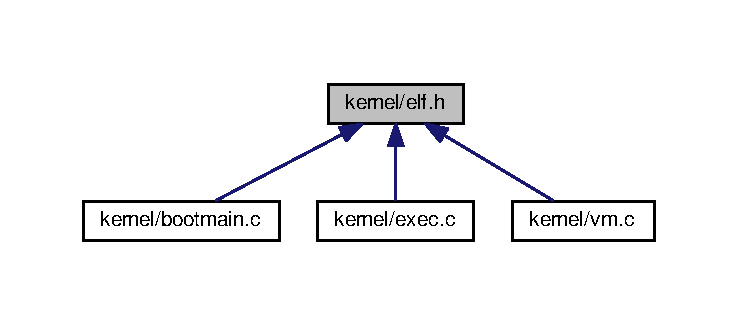
\includegraphics[width=350pt]{elf_8h__dep__incl}
\end{center}
\end{figure}
\subsection*{Data Structures}
\begin{DoxyCompactItemize}
\item 
struct \hyperlink{structelfhdr}{elfhdr}
\item 
struct \hyperlink{structproghdr}{proghdr}
\end{DoxyCompactItemize}
\subsection*{Macros}
\begin{DoxyCompactItemize}
\item 
\#define \hyperlink{elf_8h_abb1c2e5626667aacc7b3efd269a6c0eb}{E\-L\-F\-\_\-\-M\-A\-G\-I\-C}~0x464\-C457\-F\-U
\item 
\#define \hyperlink{elf_8h_a6a45c035b7a2930e62ac97a6bd8121e9}{E\-L\-F\-\_\-\-P\-R\-O\-G\-\_\-\-L\-O\-A\-D}~1
\item 
\#define \hyperlink{elf_8h_ac9608330ae745d90d7b59374fe827538}{E\-L\-F\-\_\-\-P\-R\-O\-G\-\_\-\-F\-L\-A\-G\-\_\-\-E\-X\-E\-C}~1
\item 
\#define \hyperlink{elf_8h_a18b2debb63e51b9f66a702e3625a8622}{E\-L\-F\-\_\-\-P\-R\-O\-G\-\_\-\-F\-L\-A\-G\-\_\-\-W\-R\-I\-T\-E}~2
\item 
\#define \hyperlink{elf_8h_a63df5e8bbab03913953e0042936f32c6}{E\-L\-F\-\_\-\-P\-R\-O\-G\-\_\-\-F\-L\-A\-G\-\_\-\-R\-E\-A\-D}~4
\end{DoxyCompactItemize}


\subsection{Macro Definition Documentation}
\hypertarget{elf_8h_abb1c2e5626667aacc7b3efd269a6c0eb}{\index{elf.\-h@{elf.\-h}!E\-L\-F\-\_\-\-M\-A\-G\-I\-C@{E\-L\-F\-\_\-\-M\-A\-G\-I\-C}}
\index{E\-L\-F\-\_\-\-M\-A\-G\-I\-C@{E\-L\-F\-\_\-\-M\-A\-G\-I\-C}!elf.h@{elf.\-h}}
\subsubsection[{E\-L\-F\-\_\-\-M\-A\-G\-I\-C}]{\setlength{\rightskip}{0pt plus 5cm}\#define E\-L\-F\-\_\-\-M\-A\-G\-I\-C~0x464\-C457\-F\-U}}\label{elf_8h_abb1c2e5626667aacc7b3efd269a6c0eb}


Definition at line 5 of file elf.\-h.

\hypertarget{elf_8h_ac9608330ae745d90d7b59374fe827538}{\index{elf.\-h@{elf.\-h}!E\-L\-F\-\_\-\-P\-R\-O\-G\-\_\-\-F\-L\-A\-G\-\_\-\-E\-X\-E\-C@{E\-L\-F\-\_\-\-P\-R\-O\-G\-\_\-\-F\-L\-A\-G\-\_\-\-E\-X\-E\-C}}
\index{E\-L\-F\-\_\-\-P\-R\-O\-G\-\_\-\-F\-L\-A\-G\-\_\-\-E\-X\-E\-C@{E\-L\-F\-\_\-\-P\-R\-O\-G\-\_\-\-F\-L\-A\-G\-\_\-\-E\-X\-E\-C}!elf.h@{elf.\-h}}
\subsubsection[{E\-L\-F\-\_\-\-P\-R\-O\-G\-\_\-\-F\-L\-A\-G\-\_\-\-E\-X\-E\-C}]{\setlength{\rightskip}{0pt plus 5cm}\#define E\-L\-F\-\_\-\-P\-R\-O\-G\-\_\-\-F\-L\-A\-G\-\_\-\-E\-X\-E\-C~1}}\label{elf_8h_ac9608330ae745d90d7b59374fe827538}


Definition at line 42 of file elf.\-h.

\hypertarget{elf_8h_a63df5e8bbab03913953e0042936f32c6}{\index{elf.\-h@{elf.\-h}!E\-L\-F\-\_\-\-P\-R\-O\-G\-\_\-\-F\-L\-A\-G\-\_\-\-R\-E\-A\-D@{E\-L\-F\-\_\-\-P\-R\-O\-G\-\_\-\-F\-L\-A\-G\-\_\-\-R\-E\-A\-D}}
\index{E\-L\-F\-\_\-\-P\-R\-O\-G\-\_\-\-F\-L\-A\-G\-\_\-\-R\-E\-A\-D@{E\-L\-F\-\_\-\-P\-R\-O\-G\-\_\-\-F\-L\-A\-G\-\_\-\-R\-E\-A\-D}!elf.h@{elf.\-h}}
\subsubsection[{E\-L\-F\-\_\-\-P\-R\-O\-G\-\_\-\-F\-L\-A\-G\-\_\-\-R\-E\-A\-D}]{\setlength{\rightskip}{0pt plus 5cm}\#define E\-L\-F\-\_\-\-P\-R\-O\-G\-\_\-\-F\-L\-A\-G\-\_\-\-R\-E\-A\-D~4}}\label{elf_8h_a63df5e8bbab03913953e0042936f32c6}


Definition at line 44 of file elf.\-h.

\hypertarget{elf_8h_a18b2debb63e51b9f66a702e3625a8622}{\index{elf.\-h@{elf.\-h}!E\-L\-F\-\_\-\-P\-R\-O\-G\-\_\-\-F\-L\-A\-G\-\_\-\-W\-R\-I\-T\-E@{E\-L\-F\-\_\-\-P\-R\-O\-G\-\_\-\-F\-L\-A\-G\-\_\-\-W\-R\-I\-T\-E}}
\index{E\-L\-F\-\_\-\-P\-R\-O\-G\-\_\-\-F\-L\-A\-G\-\_\-\-W\-R\-I\-T\-E@{E\-L\-F\-\_\-\-P\-R\-O\-G\-\_\-\-F\-L\-A\-G\-\_\-\-W\-R\-I\-T\-E}!elf.h@{elf.\-h}}
\subsubsection[{E\-L\-F\-\_\-\-P\-R\-O\-G\-\_\-\-F\-L\-A\-G\-\_\-\-W\-R\-I\-T\-E}]{\setlength{\rightskip}{0pt plus 5cm}\#define E\-L\-F\-\_\-\-P\-R\-O\-G\-\_\-\-F\-L\-A\-G\-\_\-\-W\-R\-I\-T\-E~2}}\label{elf_8h_a18b2debb63e51b9f66a702e3625a8622}


Definition at line 43 of file elf.\-h.

\hypertarget{elf_8h_a6a45c035b7a2930e62ac97a6bd8121e9}{\index{elf.\-h@{elf.\-h}!E\-L\-F\-\_\-\-P\-R\-O\-G\-\_\-\-L\-O\-A\-D@{E\-L\-F\-\_\-\-P\-R\-O\-G\-\_\-\-L\-O\-A\-D}}
\index{E\-L\-F\-\_\-\-P\-R\-O\-G\-\_\-\-L\-O\-A\-D@{E\-L\-F\-\_\-\-P\-R\-O\-G\-\_\-\-L\-O\-A\-D}!elf.h@{elf.\-h}}
\subsubsection[{E\-L\-F\-\_\-\-P\-R\-O\-G\-\_\-\-L\-O\-A\-D}]{\setlength{\rightskip}{0pt plus 5cm}\#define E\-L\-F\-\_\-\-P\-R\-O\-G\-\_\-\-L\-O\-A\-D~1}}\label{elf_8h_a6a45c035b7a2930e62ac97a6bd8121e9}


Definition at line 39 of file elf.\-h.


\hypertarget{exec_8c}{\section{kernel/exec.c File Reference}
\label{exec_8c}\index{kernel/exec.\-c@{kernel/exec.\-c}}
}
{\ttfamily \#include \char`\"{}types.\-h\char`\"{}}\\*
{\ttfamily \#include \char`\"{}param.\-h\char`\"{}}\\*
{\ttfamily \#include \char`\"{}mmu.\-h\char`\"{}}\\*
{\ttfamily \#include \char`\"{}proc.\-h\char`\"{}}\\*
{\ttfamily \#include \char`\"{}defs.\-h\char`\"{}}\\*
{\ttfamily \#include \char`\"{}x86.\-h\char`\"{}}\\*
{\ttfamily \#include \char`\"{}elf.\-h\char`\"{}}\\*
Include dependency graph for exec.\-c\-:
\nopagebreak
\begin{figure}[H]
\begin{center}
\leavevmode
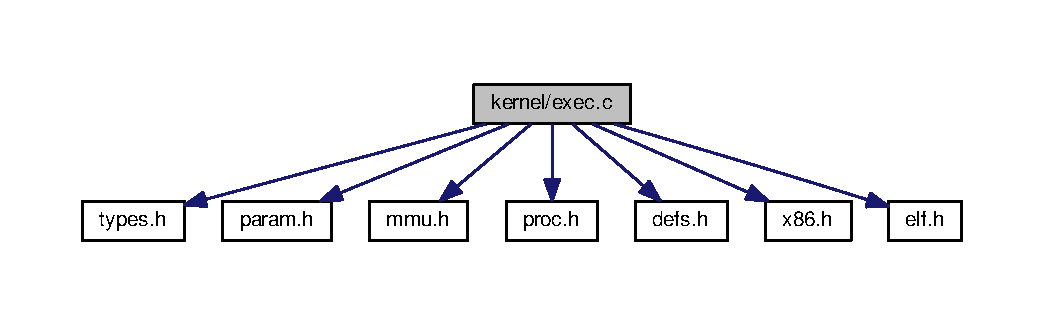
\includegraphics[width=350pt]{exec_8c__incl}
\end{center}
\end{figure}
\subsection*{Functions}
\begin{DoxyCompactItemize}
\item 
int \hyperlink{exec_8c_ace32454ed0d37834dcb1cb4f8b727e6e}{exec} (char $\ast$path, char $\ast$$\ast$\hyperlink{init_8c_abd1a2cf54950f450187ef24c1cdcac0c}{argv})
\end{DoxyCompactItemize}


\subsection{Function Documentation}
\hypertarget{exec_8c_ace32454ed0d37834dcb1cb4f8b727e6e}{\index{exec.\-c@{exec.\-c}!exec@{exec}}
\index{exec@{exec}!exec.c@{exec.\-c}}
\subsubsection[{exec}]{\setlength{\rightskip}{0pt plus 5cm}int exec (
\begin{DoxyParamCaption}
\item[{char $\ast$}]{path, }
\item[{char $\ast$$\ast$}]{argv}
\end{DoxyParamCaption}
)}}\label{exec_8c_ace32454ed0d37834dcb1cb4f8b727e6e}


Definition at line 10 of file exec.\-c.


\hypertarget{exec_8d}{\section{kernel/exec.d File Reference}
\label{exec_8d}\index{kernel/exec.\-d@{kernel/exec.\-d}}
}

\hypertarget{file_8c}{\section{kernel/file.c File Reference}
\label{file_8c}\index{kernel/file.\-c@{kernel/file.\-c}}
}
{\ttfamily \#include \char`\"{}types.\-h\char`\"{}}\\*
{\ttfamily \#include \char`\"{}defs.\-h\char`\"{}}\\*
{\ttfamily \#include \char`\"{}param.\-h\char`\"{}}\\*
{\ttfamily \#include \char`\"{}fs.\-h\char`\"{}}\\*
{\ttfamily \#include \char`\"{}file.\-h\char`\"{}}\\*
{\ttfamily \#include \char`\"{}spinlock.\-h\char`\"{}}\\*
Include dependency graph for file.\-c\-:
\nopagebreak
\begin{figure}[H]
\begin{center}
\leavevmode
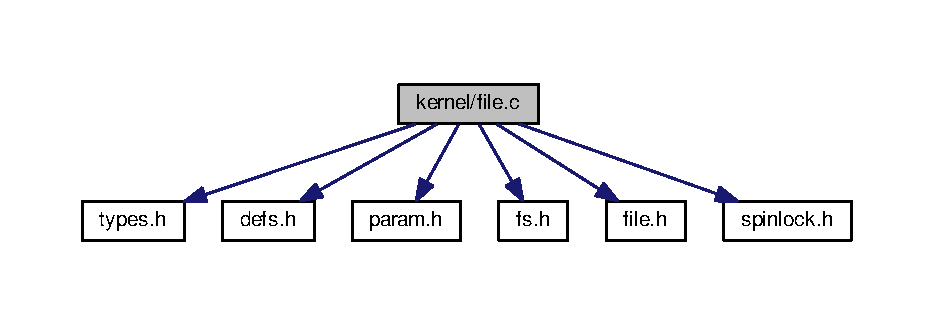
\includegraphics[width=350pt]{file_8c__incl}
\end{center}
\end{figure}
\subsection*{Functions}
\begin{DoxyCompactItemize}
\item 
void \hyperlink{file_8c_a66bb5a4b304ea0f851dd999fc8195fa4}{fileinit} (void)
\item 
struct \hyperlink{structfile}{file} $\ast$ \hyperlink{file_8c_a69d3d2dd94efa1f1ff8d0143f4d9b786}{filealloc} (void)
\item 
struct \hyperlink{structfile}{file} $\ast$ \hyperlink{file_8c_a014992e93368bee9318b5e1ff575cb91}{filedup} (struct \hyperlink{structfile}{file} $\ast$f)
\item 
void \hyperlink{file_8c_ae557c81ab89c24219146144bb6adaa2c}{fileclose} (struct \hyperlink{structfile}{file} $\ast$f)
\item 
int \hyperlink{file_8c_afff8e849fa54dea2a5a27dbb97474607}{filestat} (struct \hyperlink{structfile}{file} $\ast$f, struct \hyperlink{structstat}{stat} $\ast$st)
\item 
int \hyperlink{file_8c_a1dc8c87c7e48bdaaf98e9c7047928f29}{fileread} (struct \hyperlink{structfile}{file} $\ast$f, char $\ast$addr, int n)
\item 
int \hyperlink{file_8c_ab8de757a0a9f58dcc6511ea5e46ebb88}{filewrite} (struct \hyperlink{structfile}{file} $\ast$f, char $\ast$addr, int n)
\end{DoxyCompactItemize}
\subsection*{Variables}
\begin{DoxyCompactItemize}
\item 
struct \hyperlink{structdevsw}{devsw} \hyperlink{file_8c_aadbb32b41c0d0e9c19d6d8fa3a0a6502}{devsw} \mbox{[}\hyperlink{param_8h_aa564a41c8409694da49b0badf2bb2853}{N\-D\-E\-V}\mbox{]}
\item 
\begin{tabbing}
xx\=xx\=xx\=xx\=xx\=xx\=xx\=xx\=xx\=\kill
struct \{\\
\>struct \hyperlink{structspinlock}{spinlock} \hyperlink{file_8c_ab28e82cd5dda7d960095706a3ea20572}{lock}\\
\>struct \hyperlink{structfile}{file} \hyperlink{file_8c_a7cfa5243b3d349a415c7500c962fe9a5}{file} \mbox{[}\hyperlink{param_8h_a8485f4e81de2537e6a0935626167a775}{NFILE}\mbox{]}\\
\} \hyperlink{file_8c_a5e3713b2e8d8fca04c15e52b9a315620}{ftable}\\

\end{tabbing}\end{DoxyCompactItemize}


\subsection{Function Documentation}
\hypertarget{file_8c_a69d3d2dd94efa1f1ff8d0143f4d9b786}{\index{file.\-c@{file.\-c}!filealloc@{filealloc}}
\index{filealloc@{filealloc}!file.c@{file.\-c}}
\subsubsection[{filealloc}]{\setlength{\rightskip}{0pt plus 5cm}struct {\bf file}$\ast$ filealloc (
\begin{DoxyParamCaption}
\item[{void}]{}
\end{DoxyParamCaption}
)}}\label{file_8c_a69d3d2dd94efa1f1ff8d0143f4d9b786}


Definition at line 22 of file file.\-c.

\hypertarget{file_8c_ae557c81ab89c24219146144bb6adaa2c}{\index{file.\-c@{file.\-c}!fileclose@{fileclose}}
\index{fileclose@{fileclose}!file.c@{file.\-c}}
\subsubsection[{fileclose}]{\setlength{\rightskip}{0pt plus 5cm}void fileclose (
\begin{DoxyParamCaption}
\item[{struct {\bf file} $\ast$}]{f}
\end{DoxyParamCaption}
)}}\label{file_8c_ae557c81ab89c24219146144bb6adaa2c}


Definition at line 52 of file file.\-c.

\hypertarget{file_8c_a014992e93368bee9318b5e1ff575cb91}{\index{file.\-c@{file.\-c}!filedup@{filedup}}
\index{filedup@{filedup}!file.c@{file.\-c}}
\subsubsection[{filedup}]{\setlength{\rightskip}{0pt plus 5cm}struct {\bf file}$\ast$ filedup (
\begin{DoxyParamCaption}
\item[{struct {\bf file} $\ast$}]{f}
\end{DoxyParamCaption}
)}}\label{file_8c_a014992e93368bee9318b5e1ff575cb91}


Definition at line 40 of file file.\-c.

\hypertarget{file_8c_a66bb5a4b304ea0f851dd999fc8195fa4}{\index{file.\-c@{file.\-c}!fileinit@{fileinit}}
\index{fileinit@{fileinit}!file.c@{file.\-c}}
\subsubsection[{fileinit}]{\setlength{\rightskip}{0pt plus 5cm}void fileinit (
\begin{DoxyParamCaption}
\item[{void}]{}
\end{DoxyParamCaption}
)}}\label{file_8c_a66bb5a4b304ea0f851dd999fc8195fa4}


Definition at line 15 of file file.\-c.

\hypertarget{file_8c_a1dc8c87c7e48bdaaf98e9c7047928f29}{\index{file.\-c@{file.\-c}!fileread@{fileread}}
\index{fileread@{fileread}!file.c@{file.\-c}}
\subsubsection[{fileread}]{\setlength{\rightskip}{0pt plus 5cm}int fileread (
\begin{DoxyParamCaption}
\item[{struct {\bf file} $\ast$}]{f, }
\item[{char $\ast$}]{addr, }
\item[{int}]{n}
\end{DoxyParamCaption}
)}}\label{file_8c_a1dc8c87c7e48bdaaf98e9c7047928f29}


Definition at line 89 of file file.\-c.

\hypertarget{file_8c_afff8e849fa54dea2a5a27dbb97474607}{\index{file.\-c@{file.\-c}!filestat@{filestat}}
\index{filestat@{filestat}!file.c@{file.\-c}}
\subsubsection[{filestat}]{\setlength{\rightskip}{0pt plus 5cm}int filestat (
\begin{DoxyParamCaption}
\item[{struct {\bf file} $\ast$}]{f, }
\item[{struct {\bf stat} $\ast$}]{st}
\end{DoxyParamCaption}
)}}\label{file_8c_afff8e849fa54dea2a5a27dbb97474607}


Definition at line 76 of file file.\-c.

\hypertarget{file_8c_ab8de757a0a9f58dcc6511ea5e46ebb88}{\index{file.\-c@{file.\-c}!filewrite@{filewrite}}
\index{filewrite@{filewrite}!file.c@{file.\-c}}
\subsubsection[{filewrite}]{\setlength{\rightskip}{0pt plus 5cm}int filewrite (
\begin{DoxyParamCaption}
\item[{struct {\bf file} $\ast$}]{f, }
\item[{char $\ast$}]{addr, }
\item[{int}]{n}
\end{DoxyParamCaption}
)}}\label{file_8c_ab8de757a0a9f58dcc6511ea5e46ebb88}


Definition at line 109 of file file.\-c.



\subsection{Variable Documentation}
\hypertarget{file_8c_aadbb32b41c0d0e9c19d6d8fa3a0a6502}{\index{file.\-c@{file.\-c}!devsw@{devsw}}
\index{devsw@{devsw}!file.c@{file.\-c}}
\subsubsection[{devsw}]{\setlength{\rightskip}{0pt plus 5cm}struct {\bf devsw} {\bf devsw}\mbox{[}{\bf N\-D\-E\-V}\mbox{]}}}\label{file_8c_aadbb32b41c0d0e9c19d6d8fa3a0a6502}


Definition at line 8 of file file.\-c.

\hypertarget{file_8c_a7cfa5243b3d349a415c7500c962fe9a5}{\index{file.\-c@{file.\-c}!file@{file}}
\index{file@{file}!file.c@{file.\-c}}
\subsubsection[{file}]{\setlength{\rightskip}{0pt plus 5cm}struct {\bf file} {\bf file}\mbox{[}{\bf N\-F\-I\-L\-E}\mbox{]}}}\label{file_8c_a7cfa5243b3d349a415c7500c962fe9a5}


Definition at line 11 of file file.\-c.

\hypertarget{file_8c_a5e3713b2e8d8fca04c15e52b9a315620}{\index{file.\-c@{file.\-c}!ftable@{ftable}}
\index{ftable@{ftable}!file.c@{file.\-c}}
\subsubsection[{ftable}]{\setlength{\rightskip}{0pt plus 5cm}struct \{ ... \}   ftable}}\label{file_8c_a5e3713b2e8d8fca04c15e52b9a315620}
\hypertarget{file_8c_ab28e82cd5dda7d960095706a3ea20572}{\index{file.\-c@{file.\-c}!lock@{lock}}
\index{lock@{lock}!file.c@{file.\-c}}
\subsubsection[{lock}]{\setlength{\rightskip}{0pt plus 5cm}struct {\bf spinlock} lock}}\label{file_8c_ab28e82cd5dda7d960095706a3ea20572}


Definition at line 10 of file file.\-c.


\hypertarget{file_8d}{\section{kernel/file.d File Reference}
\label{file_8d}\index{kernel/file.\-d@{kernel/file.\-d}}
}

\hypertarget{file_8h}{\section{kernel/file.h File Reference}
\label{file_8h}\index{kernel/file.\-h@{kernel/file.\-h}}
}
This graph shows which files directly or indirectly include this file\-:
\nopagebreak
\begin{figure}[H]
\begin{center}
\leavevmode
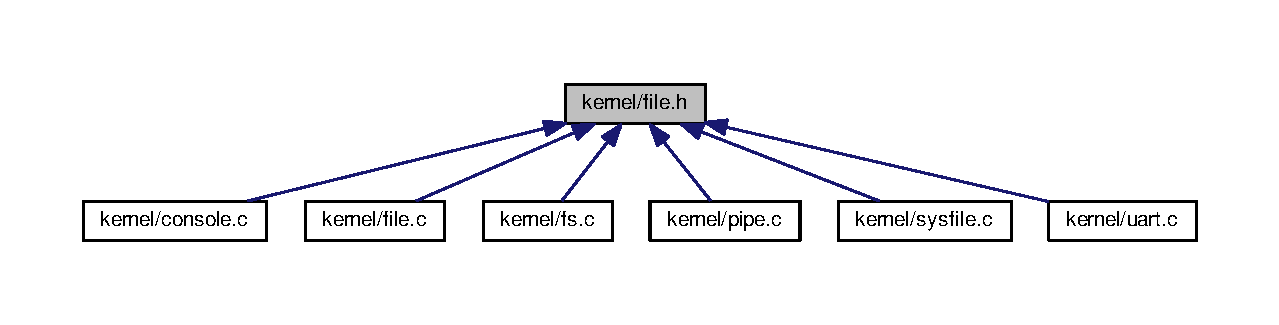
\includegraphics[width=350pt]{file_8h__dep__incl}
\end{center}
\end{figure}
\subsection*{Data Structures}
\begin{DoxyCompactItemize}
\item 
struct \hyperlink{structfile}{file}
\item 
struct \hyperlink{structinode}{inode}
\item 
struct \hyperlink{structdevsw}{devsw}
\end{DoxyCompactItemize}
\subsection*{Macros}
\begin{DoxyCompactItemize}
\item 
\#define \hyperlink{file_8h_af4d394409b02e4e177134601f77f98af}{I\-\_\-\-B\-U\-S\-Y}~0x1
\item 
\#define \hyperlink{file_8h_a986f408af8aa8e86ef5ab55463305483}{I\-\_\-\-V\-A\-L\-I\-D}~0x2
\item 
\#define \hyperlink{file_8h_a6c17169f464fb1a2995dbe06faa47a5f}{C\-O\-N\-S\-O\-L\-E}~1
\end{DoxyCompactItemize}
\subsection*{Variables}
\begin{DoxyCompactItemize}
\item 
struct \hyperlink{structdevsw}{devsw} \hyperlink{file_8h_aef498b4c2cbc1a4286c67ff5f20afec9}{devsw} \mbox{[}$\,$\mbox{]}
\end{DoxyCompactItemize}


\subsection{Macro Definition Documentation}
\hypertarget{file_8h_a6c17169f464fb1a2995dbe06faa47a5f}{\index{file.\-h@{file.\-h}!C\-O\-N\-S\-O\-L\-E@{C\-O\-N\-S\-O\-L\-E}}
\index{C\-O\-N\-S\-O\-L\-E@{C\-O\-N\-S\-O\-L\-E}!file.h@{file.\-h}}
\subsubsection[{C\-O\-N\-S\-O\-L\-E}]{\setlength{\rightskip}{0pt plus 5cm}\#define C\-O\-N\-S\-O\-L\-E~1}}\label{file_8h_a6c17169f464fb1a2995dbe06faa47a5f}


Definition at line 43 of file file.\-h.

\hypertarget{file_8h_af4d394409b02e4e177134601f77f98af}{\index{file.\-h@{file.\-h}!I\-\_\-\-B\-U\-S\-Y@{I\-\_\-\-B\-U\-S\-Y}}
\index{I\-\_\-\-B\-U\-S\-Y@{I\-\_\-\-B\-U\-S\-Y}!file.h@{file.\-h}}
\subsubsection[{I\-\_\-\-B\-U\-S\-Y}]{\setlength{\rightskip}{0pt plus 5cm}\#define I\-\_\-\-B\-U\-S\-Y~0x1}}\label{file_8h_af4d394409b02e4e177134601f77f98af}


Definition at line 30 of file file.\-h.

\hypertarget{file_8h_a986f408af8aa8e86ef5ab55463305483}{\index{file.\-h@{file.\-h}!I\-\_\-\-V\-A\-L\-I\-D@{I\-\_\-\-V\-A\-L\-I\-D}}
\index{I\-\_\-\-V\-A\-L\-I\-D@{I\-\_\-\-V\-A\-L\-I\-D}!file.h@{file.\-h}}
\subsubsection[{I\-\_\-\-V\-A\-L\-I\-D}]{\setlength{\rightskip}{0pt plus 5cm}\#define I\-\_\-\-V\-A\-L\-I\-D~0x2}}\label{file_8h_a986f408af8aa8e86ef5ab55463305483}


Definition at line 31 of file file.\-h.



\subsection{Variable Documentation}
\hypertarget{file_8h_aef498b4c2cbc1a4286c67ff5f20afec9}{\index{file.\-h@{file.\-h}!devsw@{devsw}}
\index{devsw@{devsw}!file.h@{file.\-h}}
\subsubsection[{devsw}]{\setlength{\rightskip}{0pt plus 5cm}struct {\bf devsw} {\bf devsw}\mbox{[}$\,$\mbox{]}}}\label{file_8h_aef498b4c2cbc1a4286c67ff5f20afec9}


Definition at line 8 of file file.\-c.


\hypertarget{fs_8c}{\section{kernel/fs.c File Reference}
\label{fs_8c}\index{kernel/fs.\-c@{kernel/fs.\-c}}
}
{\ttfamily \#include \char`\"{}types.\-h\char`\"{}}\\*
{\ttfamily \#include \char`\"{}defs.\-h\char`\"{}}\\*
{\ttfamily \#include \char`\"{}param.\-h\char`\"{}}\\*
{\ttfamily \#include \char`\"{}stat.\-h\char`\"{}}\\*
{\ttfamily \#include \char`\"{}mmu.\-h\char`\"{}}\\*
{\ttfamily \#include \char`\"{}proc.\-h\char`\"{}}\\*
{\ttfamily \#include \char`\"{}spinlock.\-h\char`\"{}}\\*
{\ttfamily \#include \char`\"{}buf.\-h\char`\"{}}\\*
{\ttfamily \#include \char`\"{}fs.\-h\char`\"{}}\\*
{\ttfamily \#include \char`\"{}file.\-h\char`\"{}}\\*
Include dependency graph for fs.\-c\-:
\nopagebreak
\begin{figure}[H]
\begin{center}
\leavevmode
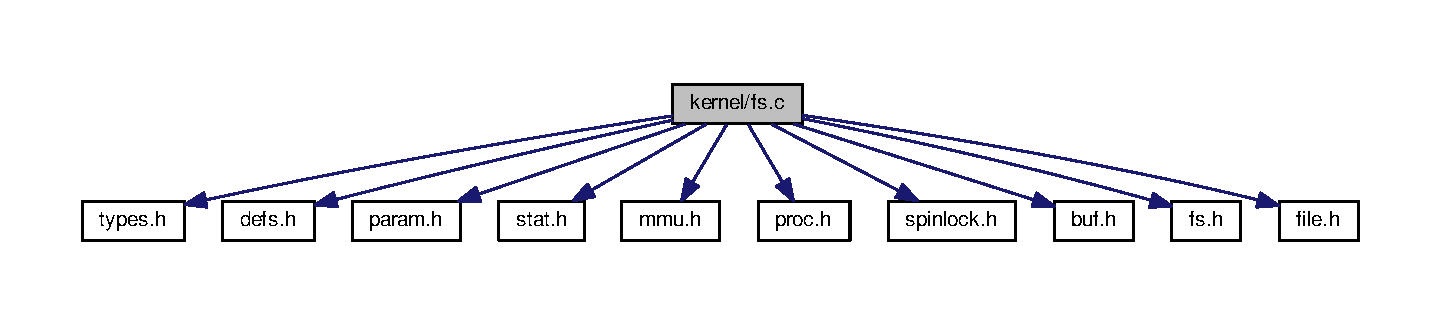
\includegraphics[width=350pt]{fs_8c__incl}
\end{center}
\end{figure}
\subsection*{Macros}
\begin{DoxyCompactItemize}
\item 
\#define \hyperlink{fs_8c_ac6afabdc09a49a433ee19d8a9486056d}{min}(a, b)~((a) $<$ (b) ? (a) \-: (b))
\end{DoxyCompactItemize}
\subsection*{Functions}
\begin{DoxyCompactItemize}
\item 
void \hyperlink{fs_8c_a508e2b44186d5b3997a1564fe5a6c2d9}{iinit} (void)
\item 
struct \hyperlink{structinode}{inode} $\ast$ \hyperlink{fs_8c_adb360ce0b70a32d19d089fba4cd91293}{ialloc} (\hyperlink{types_8h_a91ad9478d81a7aaf2593e8d9c3d06a14}{uint} dev, short type)
\item 
void \hyperlink{fs_8c_a7220afa8e5f4bea540eb95879ea7df6e}{iupdate} (struct \hyperlink{structinode}{inode} $\ast$ip)
\item 
struct \hyperlink{structinode}{inode} $\ast$ \hyperlink{fs_8c_a6b41577cc09b2a009be8f84bfb500079}{idup} (struct \hyperlink{structinode}{inode} $\ast$ip)
\item 
void \hyperlink{fs_8c_aed28187406d84a3aa71f10c6235a03ec}{ilock} (struct \hyperlink{structinode}{inode} $\ast$ip)
\item 
void \hyperlink{fs_8c_ae4e29916219b9293b37f9c34220694fe}{iunlock} (struct \hyperlink{structinode}{inode} $\ast$ip)
\item 
void \hyperlink{fs_8c_ab3c447f135c68e4c3c1f8d5866f6e77b}{iput} (struct \hyperlink{structinode}{inode} $\ast$ip)
\item 
void \hyperlink{fs_8c_a207b3008bae35596c55ec7c4fc6875eb}{iunlockput} (struct \hyperlink{structinode}{inode} $\ast$ip)
\item 
void \hyperlink{fs_8c_a4ccff0bd4d9802e709d0af8d71a59861}{stati} (struct \hyperlink{structinode}{inode} $\ast$ip, struct \hyperlink{structstat}{stat} $\ast$st)
\item 
int \hyperlink{fs_8c_a3aba1fa9f6789d09356aec5b96d91fa8}{readi} (struct \hyperlink{structinode}{inode} $\ast$ip, char $\ast$dst, \hyperlink{types_8h_a91ad9478d81a7aaf2593e8d9c3d06a14}{uint} off, \hyperlink{types_8h_a91ad9478d81a7aaf2593e8d9c3d06a14}{uint} n)
\item 
int \hyperlink{fs_8c_a15858f4d8a4cc1def3d84d03c312836b}{writei} (struct \hyperlink{structinode}{inode} $\ast$ip, char $\ast$src, \hyperlink{types_8h_a91ad9478d81a7aaf2593e8d9c3d06a14}{uint} off, \hyperlink{types_8h_a91ad9478d81a7aaf2593e8d9c3d06a14}{uint} n)
\item 
int \hyperlink{fs_8c_ae74f6e5b19a4e7f3e72807ee67141819}{namecmp} (const char $\ast$s, const char $\ast$t)
\item 
struct \hyperlink{structinode}{inode} $\ast$ \hyperlink{fs_8c_aa182c62fade7a0bae9408830d5e06d4f}{dirlookup} (struct \hyperlink{structinode}{inode} $\ast$dp, char $\ast$\hyperlink{usertests_8c_aee754febd402311e2a552cb0d6ab6629}{name}, \hyperlink{types_8h_a91ad9478d81a7aaf2593e8d9c3d06a14}{uint} $\ast$poff)
\item 
int \hyperlink{fs_8c_a69a135a0e8a06d9f306d77ebc0c1f7a0}{dirlink} (struct \hyperlink{structinode}{inode} $\ast$dp, char $\ast$\hyperlink{usertests_8c_aee754febd402311e2a552cb0d6ab6629}{name}, \hyperlink{types_8h_a91ad9478d81a7aaf2593e8d9c3d06a14}{uint} inum)
\item 
struct \hyperlink{structinode}{inode} $\ast$ \hyperlink{fs_8c_a9baba030d5bc6e9e20cf8b7d181edf35}{namei} (char $\ast$path)
\item 
struct \hyperlink{structinode}{inode} $\ast$ \hyperlink{fs_8c_a5a987ca4f8ffd579b96a8b9a60e61a7c}{nameiparent} (char $\ast$path, char $\ast$\hyperlink{usertests_8c_aee754febd402311e2a552cb0d6ab6629}{name})
\end{DoxyCompactItemize}
\subsection*{Variables}
\begin{DoxyCompactItemize}
\item 
\begin{tabbing}
xx\=xx\=xx\=xx\=xx\=xx\=xx\=xx\=xx\=\kill
struct \{\\
\>struct \hyperlink{structspinlock}{spinlock} \hyperlink{fs_8c_ab28e82cd5dda7d960095706a3ea20572}{lock}\\
\>struct \hyperlink{structinode}{inode} \hyperlink{fs_8c_a6baaf26dd83b71b8d684c5d54a709e31}{inode} \mbox{[}\hyperlink{param_8h_adabafa10c7951be7c875cd2ee212be85}{NINODE}\mbox{]}\\
\} \hyperlink{fs_8c_a1fbfdebf96af7ed1f992e387cba059b3}{icache}\\

\end{tabbing}\end{DoxyCompactItemize}


\subsection{Macro Definition Documentation}
\hypertarget{fs_8c_ac6afabdc09a49a433ee19d8a9486056d}{\index{fs.\-c@{fs.\-c}!min@{min}}
\index{min@{min}!fs.c@{fs.\-c}}
\subsubsection[{min}]{\setlength{\rightskip}{0pt plus 5cm}\#define min(
\begin{DoxyParamCaption}
\item[{}]{a, }
\item[{}]{b}
\end{DoxyParamCaption}
)~((a) $<$ (b) ? (a) \-: (b))}}\label{fs_8c_ac6afabdc09a49a433ee19d8a9486056d}


Definition at line 24 of file fs.\-c.



\subsection{Function Documentation}
\hypertarget{fs_8c_a69a135a0e8a06d9f306d77ebc0c1f7a0}{\index{fs.\-c@{fs.\-c}!dirlink@{dirlink}}
\index{dirlink@{dirlink}!fs.c@{fs.\-c}}
\subsubsection[{dirlink}]{\setlength{\rightskip}{0pt plus 5cm}int dirlink (
\begin{DoxyParamCaption}
\item[{struct {\bf inode} $\ast$}]{dp, }
\item[{char $\ast$}]{name, }
\item[{{\bf uint}}]{inum}
\end{DoxyParamCaption}
)}}\label{fs_8c_a69a135a0e8a06d9f306d77ebc0c1f7a0}


Definition at line 497 of file fs.\-c.

\hypertarget{fs_8c_aa182c62fade7a0bae9408830d5e06d4f}{\index{fs.\-c@{fs.\-c}!dirlookup@{dirlookup}}
\index{dirlookup@{dirlookup}!fs.c@{fs.\-c}}
\subsubsection[{dirlookup}]{\setlength{\rightskip}{0pt plus 5cm}struct {\bf inode}$\ast$ dirlookup (
\begin{DoxyParamCaption}
\item[{struct {\bf inode} $\ast$}]{dp, }
\item[{char $\ast$}]{name, }
\item[{{\bf uint} $\ast$}]{poff}
\end{DoxyParamCaption}
)}}\label{fs_8c_aa182c62fade7a0bae9408830d5e06d4f}


Definition at line 465 of file fs.\-c.

\hypertarget{fs_8c_adb360ce0b70a32d19d089fba4cd91293}{\index{fs.\-c@{fs.\-c}!ialloc@{ialloc}}
\index{ialloc@{ialloc}!fs.c@{fs.\-c}}
\subsubsection[{ialloc}]{\setlength{\rightskip}{0pt plus 5cm}struct {\bf inode}$\ast$ ialloc (
\begin{DoxyParamCaption}
\item[{{\bf uint}}]{dev, }
\item[{short}]{type}
\end{DoxyParamCaption}
)}}\label{fs_8c_adb360ce0b70a32d19d089fba4cd91293}


Definition at line 147 of file fs.\-c.

\hypertarget{fs_8c_a6b41577cc09b2a009be8f84bfb500079}{\index{fs.\-c@{fs.\-c}!idup@{idup}}
\index{idup@{idup}!fs.c@{fs.\-c}}
\subsubsection[{idup}]{\setlength{\rightskip}{0pt plus 5cm}struct {\bf inode}$\ast$ idup (
\begin{DoxyParamCaption}
\item[{struct {\bf inode} $\ast$}]{ip}
\end{DoxyParamCaption}
)}}\label{fs_8c_a6b41577cc09b2a009be8f84bfb500079}


Definition at line 227 of file fs.\-c.

\hypertarget{fs_8c_a508e2b44186d5b3997a1564fe5a6c2d9}{\index{fs.\-c@{fs.\-c}!iinit@{iinit}}
\index{iinit@{iinit}!fs.c@{fs.\-c}}
\subsubsection[{iinit}]{\setlength{\rightskip}{0pt plus 5cm}void iinit (
\begin{DoxyParamCaption}
\item[{void}]{}
\end{DoxyParamCaption}
)}}\label{fs_8c_a508e2b44186d5b3997a1564fe5a6c2d9}


Definition at line 138 of file fs.\-c.

\hypertarget{fs_8c_aed28187406d84a3aa71f10c6235a03ec}{\index{fs.\-c@{fs.\-c}!ilock@{ilock}}
\index{ilock@{ilock}!fs.c@{fs.\-c}}
\subsubsection[{ilock}]{\setlength{\rightskip}{0pt plus 5cm}void ilock (
\begin{DoxyParamCaption}
\item[{struct {\bf inode} $\ast$}]{ip}
\end{DoxyParamCaption}
)}}\label{fs_8c_aed28187406d84a3aa71f10c6235a03ec}


Definition at line 237 of file fs.\-c.

\hypertarget{fs_8c_ab3c447f135c68e4c3c1f8d5866f6e77b}{\index{fs.\-c@{fs.\-c}!iput@{iput}}
\index{iput@{iput}!fs.c@{fs.\-c}}
\subsubsection[{iput}]{\setlength{\rightskip}{0pt plus 5cm}void iput (
\begin{DoxyParamCaption}
\item[{struct {\bf inode} $\ast$}]{ip}
\end{DoxyParamCaption}
)}}\label{fs_8c_ab3c447f135c68e4c3c1f8d5866f6e77b}


Definition at line 282 of file fs.\-c.

\hypertarget{fs_8c_ae4e29916219b9293b37f9c34220694fe}{\index{fs.\-c@{fs.\-c}!iunlock@{iunlock}}
\index{iunlock@{iunlock}!fs.c@{fs.\-c}}
\subsubsection[{iunlock}]{\setlength{\rightskip}{0pt plus 5cm}void iunlock (
\begin{DoxyParamCaption}
\item[{struct {\bf inode} $\ast$}]{ip}
\end{DoxyParamCaption}
)}}\label{fs_8c_ae4e29916219b9293b37f9c34220694fe}


Definition at line 269 of file fs.\-c.

\hypertarget{fs_8c_a207b3008bae35596c55ec7c4fc6875eb}{\index{fs.\-c@{fs.\-c}!iunlockput@{iunlockput}}
\index{iunlockput@{iunlockput}!fs.c@{fs.\-c}}
\subsubsection[{iunlockput}]{\setlength{\rightskip}{0pt plus 5cm}void iunlockput (
\begin{DoxyParamCaption}
\item[{struct {\bf inode} $\ast$}]{ip}
\end{DoxyParamCaption}
)}}\label{fs_8c_a207b3008bae35596c55ec7c4fc6875eb}


Definition at line 304 of file fs.\-c.

\hypertarget{fs_8c_a7220afa8e5f4bea540eb95879ea7df6e}{\index{fs.\-c@{fs.\-c}!iupdate@{iupdate}}
\index{iupdate@{iupdate}!fs.c@{fs.\-c}}
\subsubsection[{iupdate}]{\setlength{\rightskip}{0pt plus 5cm}void iupdate (
\begin{DoxyParamCaption}
\item[{struct {\bf inode} $\ast$}]{ip}
\end{DoxyParamCaption}
)}}\label{fs_8c_a7220afa8e5f4bea540eb95879ea7df6e}


Definition at line 172 of file fs.\-c.

\hypertarget{fs_8c_ae74f6e5b19a4e7f3e72807ee67141819}{\index{fs.\-c@{fs.\-c}!namecmp@{namecmp}}
\index{namecmp@{namecmp}!fs.c@{fs.\-c}}
\subsubsection[{namecmp}]{\setlength{\rightskip}{0pt plus 5cm}int namecmp (
\begin{DoxyParamCaption}
\item[{const char $\ast$}]{s, }
\item[{const char $\ast$}]{t}
\end{DoxyParamCaption}
)}}\label{fs_8c_ae74f6e5b19a4e7f3e72807ee67141819}


Definition at line 456 of file fs.\-c.

\hypertarget{fs_8c_a9baba030d5bc6e9e20cf8b7d181edf35}{\index{fs.\-c@{fs.\-c}!namei@{namei}}
\index{namei@{namei}!fs.c@{fs.\-c}}
\subsubsection[{namei}]{\setlength{\rightskip}{0pt plus 5cm}struct {\bf inode}$\ast$ namei (
\begin{DoxyParamCaption}
\item[{char $\ast$}]{path}
\end{DoxyParamCaption}
)}}\label{fs_8c_a9baba030d5bc6e9e20cf8b7d181edf35}


Definition at line 603 of file fs.\-c.

\hypertarget{fs_8c_a5a987ca4f8ffd579b96a8b9a60e61a7c}{\index{fs.\-c@{fs.\-c}!nameiparent@{nameiparent}}
\index{nameiparent@{nameiparent}!fs.c@{fs.\-c}}
\subsubsection[{nameiparent}]{\setlength{\rightskip}{0pt plus 5cm}struct {\bf inode}$\ast$ nameiparent (
\begin{DoxyParamCaption}
\item[{char $\ast$}]{path, }
\item[{char $\ast$}]{name}
\end{DoxyParamCaption}
)}}\label{fs_8c_a5a987ca4f8ffd579b96a8b9a60e61a7c}


Definition at line 610 of file fs.\-c.

\hypertarget{fs_8c_a3aba1fa9f6789d09356aec5b96d91fa8}{\index{fs.\-c@{fs.\-c}!readi@{readi}}
\index{readi@{readi}!fs.c@{fs.\-c}}
\subsubsection[{readi}]{\setlength{\rightskip}{0pt plus 5cm}int readi (
\begin{DoxyParamCaption}
\item[{struct {\bf inode} $\ast$}]{ip, }
\item[{char $\ast$}]{dst, }
\item[{{\bf uint}}]{off, }
\item[{{\bf uint}}]{n}
\end{DoxyParamCaption}
)}}\label{fs_8c_a3aba1fa9f6789d09356aec5b96d91fa8}


Definition at line 395 of file fs.\-c.

\hypertarget{fs_8c_a4ccff0bd4d9802e709d0af8d71a59861}{\index{fs.\-c@{fs.\-c}!stati@{stati}}
\index{stati@{stati}!fs.c@{fs.\-c}}
\subsubsection[{stati}]{\setlength{\rightskip}{0pt plus 5cm}void stati (
\begin{DoxyParamCaption}
\item[{struct {\bf inode} $\ast$}]{ip, }
\item[{struct {\bf stat} $\ast$}]{st}
\end{DoxyParamCaption}
)}}\label{fs_8c_a4ccff0bd4d9802e709d0af8d71a59861}


Definition at line 384 of file fs.\-c.

\hypertarget{fs_8c_a15858f4d8a4cc1def3d84d03c312836b}{\index{fs.\-c@{fs.\-c}!writei@{writei}}
\index{writei@{writei}!fs.c@{fs.\-c}}
\subsubsection[{writei}]{\setlength{\rightskip}{0pt plus 5cm}int writei (
\begin{DoxyParamCaption}
\item[{struct {\bf inode} $\ast$}]{ip, }
\item[{char $\ast$}]{src, }
\item[{{\bf uint}}]{off, }
\item[{{\bf uint}}]{n}
\end{DoxyParamCaption}
)}}\label{fs_8c_a15858f4d8a4cc1def3d84d03c312836b}


Definition at line 422 of file fs.\-c.



\subsection{Variable Documentation}
\hypertarget{fs_8c_a1fbfdebf96af7ed1f992e387cba059b3}{\index{fs.\-c@{fs.\-c}!icache@{icache}}
\index{icache@{icache}!fs.c@{fs.\-c}}
\subsubsection[{icache}]{\setlength{\rightskip}{0pt plus 5cm}struct \{ ... \}   icache}}\label{fs_8c_a1fbfdebf96af7ed1f992e387cba059b3}
\hypertarget{fs_8c_a6baaf26dd83b71b8d684c5d54a709e31}{\index{fs.\-c@{fs.\-c}!inode@{inode}}
\index{inode@{inode}!fs.c@{fs.\-c}}
\subsubsection[{inode}]{\setlength{\rightskip}{0pt plus 5cm}struct {\bf inode} {\bf inode}\mbox{[}{\bf N\-I\-N\-O\-D\-E}\mbox{]}}}\label{fs_8c_a6baaf26dd83b71b8d684c5d54a709e31}


Definition at line 134 of file fs.\-c.

\hypertarget{fs_8c_ab28e82cd5dda7d960095706a3ea20572}{\index{fs.\-c@{fs.\-c}!lock@{lock}}
\index{lock@{lock}!fs.c@{fs.\-c}}
\subsubsection[{lock}]{\setlength{\rightskip}{0pt plus 5cm}struct {\bf spinlock} lock}}\label{fs_8c_ab28e82cd5dda7d960095706a3ea20572}


Definition at line 133 of file fs.\-c.


\hypertarget{fs_8d}{\section{kernel/fs.d File Reference}
\label{fs_8d}\index{kernel/fs.\-d@{kernel/fs.\-d}}
}

\hypertarget{ide_8c}{\section{kernel/ide.c File Reference}
\label{ide_8c}\index{kernel/ide.\-c@{kernel/ide.\-c}}
}
{\ttfamily \#include \char`\"{}types.\-h\char`\"{}}\\*
{\ttfamily \#include \char`\"{}defs.\-h\char`\"{}}\\*
{\ttfamily \#include \char`\"{}param.\-h\char`\"{}}\\*
{\ttfamily \#include \char`\"{}mmu.\-h\char`\"{}}\\*
{\ttfamily \#include \char`\"{}proc.\-h\char`\"{}}\\*
{\ttfamily \#include \char`\"{}x86.\-h\char`\"{}}\\*
{\ttfamily \#include \char`\"{}traps.\-h\char`\"{}}\\*
{\ttfamily \#include \char`\"{}spinlock.\-h\char`\"{}}\\*
{\ttfamily \#include \char`\"{}buf.\-h\char`\"{}}\\*
Include dependency graph for ide.\-c\-:
\nopagebreak
\begin{figure}[H]
\begin{center}
\leavevmode
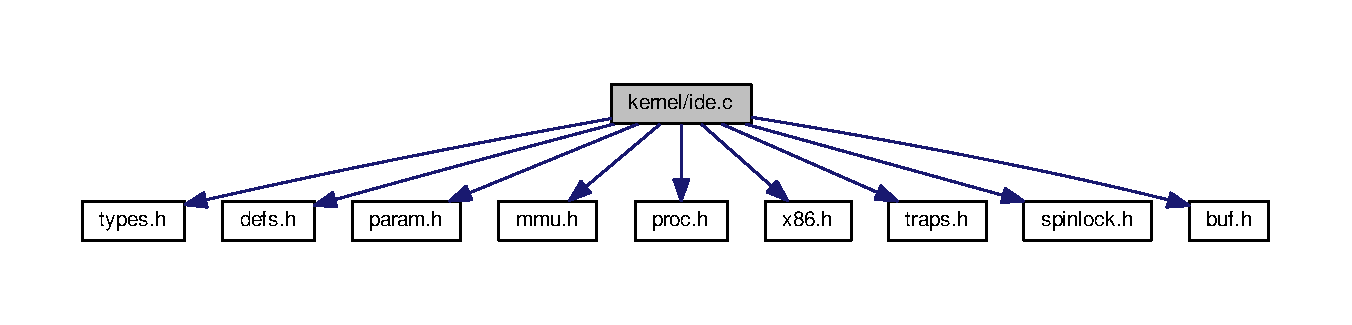
\includegraphics[width=350pt]{ide_8c__incl}
\end{center}
\end{figure}
\subsection*{Macros}
\begin{DoxyCompactItemize}
\item 
\#define \hyperlink{ide_8c_aebe5f7f39eb6d658f4a430936dc1dfc2}{I\-D\-E\-\_\-\-B\-S\-Y}~0x80
\item 
\#define \hyperlink{ide_8c_a46b51ed8423e20960b46bd4451aad66b}{I\-D\-E\-\_\-\-D\-R\-D\-Y}~0x40
\item 
\#define \hyperlink{ide_8c_a8856c5f8e07087f4cc462dc093539f75}{I\-D\-E\-\_\-\-D\-F}~0x20
\item 
\#define \hyperlink{ide_8c_ae27406a5efbf146eebd69751e36b1d14}{I\-D\-E\-\_\-\-E\-R\-R}~0x01
\item 
\#define \hyperlink{ide_8c_ae117ee5b71546241f52d9088c0fffadc}{I\-D\-E\-\_\-\-C\-M\-D\-\_\-\-R\-E\-A\-D}~0x20
\item 
\#define \hyperlink{ide_8c_ae7cbfd899670e7987022c3bb639e568d}{I\-D\-E\-\_\-\-C\-M\-D\-\_\-\-W\-R\-I\-T\-E}~0x30
\end{DoxyCompactItemize}
\subsection*{Functions}
\begin{DoxyCompactItemize}
\item 
void \hyperlink{ide_8c_aefb190a6104cb58c0bc1f8fec88d1307}{ideinit} (void)
\item 
void \hyperlink{ide_8c_a709693afdb9b89d848e684e7acde1f8f}{ideintr} (void)
\item 
void \hyperlink{ide_8c_a7f36b008f02088c86f76e98e05b55af5}{iderw} (struct \hyperlink{structbuf}{buf} $\ast$b)
\end{DoxyCompactItemize}


\subsection{Macro Definition Documentation}
\hypertarget{ide_8c_aebe5f7f39eb6d658f4a430936dc1dfc2}{\index{ide.\-c@{ide.\-c}!I\-D\-E\-\_\-\-B\-S\-Y@{I\-D\-E\-\_\-\-B\-S\-Y}}
\index{I\-D\-E\-\_\-\-B\-S\-Y@{I\-D\-E\-\_\-\-B\-S\-Y}!ide.c@{ide.\-c}}
\subsubsection[{I\-D\-E\-\_\-\-B\-S\-Y}]{\setlength{\rightskip}{0pt plus 5cm}\#define I\-D\-E\-\_\-\-B\-S\-Y~0x80}}\label{ide_8c_aebe5f7f39eb6d658f4a430936dc1dfc2}


Definition at line 13 of file ide.\-c.

\hypertarget{ide_8c_ae117ee5b71546241f52d9088c0fffadc}{\index{ide.\-c@{ide.\-c}!I\-D\-E\-\_\-\-C\-M\-D\-\_\-\-R\-E\-A\-D@{I\-D\-E\-\_\-\-C\-M\-D\-\_\-\-R\-E\-A\-D}}
\index{I\-D\-E\-\_\-\-C\-M\-D\-\_\-\-R\-E\-A\-D@{I\-D\-E\-\_\-\-C\-M\-D\-\_\-\-R\-E\-A\-D}!ide.c@{ide.\-c}}
\subsubsection[{I\-D\-E\-\_\-\-C\-M\-D\-\_\-\-R\-E\-A\-D}]{\setlength{\rightskip}{0pt plus 5cm}\#define I\-D\-E\-\_\-\-C\-M\-D\-\_\-\-R\-E\-A\-D~0x20}}\label{ide_8c_ae117ee5b71546241f52d9088c0fffadc}


Definition at line 18 of file ide.\-c.

\hypertarget{ide_8c_ae7cbfd899670e7987022c3bb639e568d}{\index{ide.\-c@{ide.\-c}!I\-D\-E\-\_\-\-C\-M\-D\-\_\-\-W\-R\-I\-T\-E@{I\-D\-E\-\_\-\-C\-M\-D\-\_\-\-W\-R\-I\-T\-E}}
\index{I\-D\-E\-\_\-\-C\-M\-D\-\_\-\-W\-R\-I\-T\-E@{I\-D\-E\-\_\-\-C\-M\-D\-\_\-\-W\-R\-I\-T\-E}!ide.c@{ide.\-c}}
\subsubsection[{I\-D\-E\-\_\-\-C\-M\-D\-\_\-\-W\-R\-I\-T\-E}]{\setlength{\rightskip}{0pt plus 5cm}\#define I\-D\-E\-\_\-\-C\-M\-D\-\_\-\-W\-R\-I\-T\-E~0x30}}\label{ide_8c_ae7cbfd899670e7987022c3bb639e568d}


Definition at line 19 of file ide.\-c.

\hypertarget{ide_8c_a8856c5f8e07087f4cc462dc093539f75}{\index{ide.\-c@{ide.\-c}!I\-D\-E\-\_\-\-D\-F@{I\-D\-E\-\_\-\-D\-F}}
\index{I\-D\-E\-\_\-\-D\-F@{I\-D\-E\-\_\-\-D\-F}!ide.c@{ide.\-c}}
\subsubsection[{I\-D\-E\-\_\-\-D\-F}]{\setlength{\rightskip}{0pt plus 5cm}\#define I\-D\-E\-\_\-\-D\-F~0x20}}\label{ide_8c_a8856c5f8e07087f4cc462dc093539f75}


Definition at line 15 of file ide.\-c.

\hypertarget{ide_8c_a46b51ed8423e20960b46bd4451aad66b}{\index{ide.\-c@{ide.\-c}!I\-D\-E\-\_\-\-D\-R\-D\-Y@{I\-D\-E\-\_\-\-D\-R\-D\-Y}}
\index{I\-D\-E\-\_\-\-D\-R\-D\-Y@{I\-D\-E\-\_\-\-D\-R\-D\-Y}!ide.c@{ide.\-c}}
\subsubsection[{I\-D\-E\-\_\-\-D\-R\-D\-Y}]{\setlength{\rightskip}{0pt plus 5cm}\#define I\-D\-E\-\_\-\-D\-R\-D\-Y~0x40}}\label{ide_8c_a46b51ed8423e20960b46bd4451aad66b}


Definition at line 14 of file ide.\-c.

\hypertarget{ide_8c_ae27406a5efbf146eebd69751e36b1d14}{\index{ide.\-c@{ide.\-c}!I\-D\-E\-\_\-\-E\-R\-R@{I\-D\-E\-\_\-\-E\-R\-R}}
\index{I\-D\-E\-\_\-\-E\-R\-R@{I\-D\-E\-\_\-\-E\-R\-R}!ide.c@{ide.\-c}}
\subsubsection[{I\-D\-E\-\_\-\-E\-R\-R}]{\setlength{\rightskip}{0pt plus 5cm}\#define I\-D\-E\-\_\-\-E\-R\-R~0x01}}\label{ide_8c_ae27406a5efbf146eebd69751e36b1d14}


Definition at line 16 of file ide.\-c.



\subsection{Function Documentation}
\hypertarget{ide_8c_aefb190a6104cb58c0bc1f8fec88d1307}{\index{ide.\-c@{ide.\-c}!ideinit@{ideinit}}
\index{ideinit@{ideinit}!ide.c@{ide.\-c}}
\subsubsection[{ideinit}]{\setlength{\rightskip}{0pt plus 5cm}void ideinit (
\begin{DoxyParamCaption}
\item[{void}]{}
\end{DoxyParamCaption}
)}}\label{ide_8c_aefb190a6104cb58c0bc1f8fec88d1307}


Definition at line 45 of file ide.\-c.

\hypertarget{ide_8c_a709693afdb9b89d848e684e7acde1f8f}{\index{ide.\-c@{ide.\-c}!ideintr@{ideintr}}
\index{ideintr@{ideintr}!ide.c@{ide.\-c}}
\subsubsection[{ideintr}]{\setlength{\rightskip}{0pt plus 5cm}void ideintr (
\begin{DoxyParamCaption}
\item[{void}]{}
\end{DoxyParamCaption}
)}}\label{ide_8c_a709693afdb9b89d848e684e7acde1f8f}


Definition at line 91 of file ide.\-c.

\hypertarget{ide_8c_a7f36b008f02088c86f76e98e05b55af5}{\index{ide.\-c@{ide.\-c}!iderw@{iderw}}
\index{iderw@{iderw}!ide.c@{ide.\-c}}
\subsubsection[{iderw}]{\setlength{\rightskip}{0pt plus 5cm}void iderw (
\begin{DoxyParamCaption}
\item[{struct {\bf buf} $\ast$}]{b}
\end{DoxyParamCaption}
)}}\label{ide_8c_a7f36b008f02088c86f76e98e05b55af5}


Definition at line 124 of file ide.\-c.


\hypertarget{ide_8d}{\section{kernel/ide.d File Reference}
\label{ide_8d}\index{kernel/ide.\-d@{kernel/ide.\-d}}
}

\hypertarget{initcode_8d}{\section{kernel/initcode.d File Reference}
\label{initcode_8d}\index{kernel/initcode.\-d@{kernel/initcode.\-d}}
}

\hypertarget{ioapic_8c}{\section{kernel/ioapic.c File Reference}
\label{ioapic_8c}\index{kernel/ioapic.\-c@{kernel/ioapic.\-c}}
}
{\ttfamily \#include \char`\"{}types.\-h\char`\"{}}\\*
{\ttfamily \#include \char`\"{}defs.\-h\char`\"{}}\\*
{\ttfamily \#include \char`\"{}traps.\-h\char`\"{}}\\*
Include dependency graph for ioapic.\-c\-:
\nopagebreak
\begin{figure}[H]
\begin{center}
\leavevmode
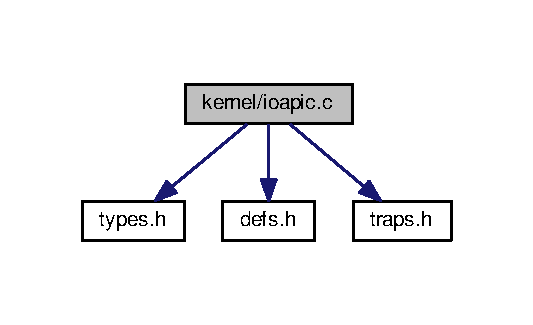
\includegraphics[width=256pt]{ioapic_8c__incl}
\end{center}
\end{figure}
\subsection*{Data Structures}
\begin{DoxyCompactItemize}
\item 
struct \hyperlink{structioapic}{ioapic}
\end{DoxyCompactItemize}
\subsection*{Macros}
\begin{DoxyCompactItemize}
\item 
\#define \hyperlink{ioapic_8c_a7d40119d2e49f7d8ae65520ccad99a1e}{I\-O\-A\-P\-I\-C}~0x\-F\-E\-C00000
\item 
\#define \hyperlink{ioapic_8c_a91339a8293cb53b81407c016bc41e2b1}{R\-E\-G\-\_\-\-I\-D}~0x00
\item 
\#define \hyperlink{ioapic_8c_ac56cc95ec46071699b119b24d6d808f9}{R\-E\-G\-\_\-\-V\-E\-R}~0x01
\item 
\#define \hyperlink{ioapic_8c_ad31b206e97e5e8cc5c70f8713669b27f}{R\-E\-G\-\_\-\-T\-A\-B\-L\-E}~0x10
\item 
\#define \hyperlink{ioapic_8c_ab26e186261a82b907e024126fafbff1f}{I\-N\-T\-\_\-\-D\-I\-S\-A\-B\-L\-E\-D}~0x00010000
\item 
\#define \hyperlink{ioapic_8c_aed01298d37e73ed9737c8a6b70e67caa}{I\-N\-T\-\_\-\-L\-E\-V\-E\-L}~0x00008000
\item 
\#define \hyperlink{ioapic_8c_a516778548109f98ff313d8753d030d37}{I\-N\-T\-\_\-\-A\-C\-T\-I\-V\-E\-L\-O\-W}~0x00002000
\item 
\#define \hyperlink{ioapic_8c_a7e41b4c95cc235d58d7a45411541f9de}{I\-N\-T\-\_\-\-L\-O\-G\-I\-C\-A\-L}~0x00000800
\end{DoxyCompactItemize}
\subsection*{Functions}
\begin{DoxyCompactItemize}
\item 
void \hyperlink{ioapic_8c_abce023b98422f397abdb425b20c8ceec}{ioapicinit} (void)
\item 
void \hyperlink{ioapic_8c_a9688537a0879e9e2ac5a90184e2ef987}{ioapicenable} (int irq, int \hyperlink{lapic_8c_ad07bc98847d46ba9772ab5ad4f52e6ec}{cpunum})
\end{DoxyCompactItemize}
\subsection*{Variables}
\begin{DoxyCompactItemize}
\item 
volatile struct \hyperlink{structioapic}{ioapic} $\ast$ \hyperlink{ioapic_8c_a61d7da24dba0ce35323deb8bb6cf6f91}{ioapic}
\end{DoxyCompactItemize}


\subsection{Macro Definition Documentation}
\hypertarget{ioapic_8c_a516778548109f98ff313d8753d030d37}{\index{ioapic.\-c@{ioapic.\-c}!I\-N\-T\-\_\-\-A\-C\-T\-I\-V\-E\-L\-O\-W@{I\-N\-T\-\_\-\-A\-C\-T\-I\-V\-E\-L\-O\-W}}
\index{I\-N\-T\-\_\-\-A\-C\-T\-I\-V\-E\-L\-O\-W@{I\-N\-T\-\_\-\-A\-C\-T\-I\-V\-E\-L\-O\-W}!ioapic.c@{ioapic.\-c}}
\subsubsection[{I\-N\-T\-\_\-\-A\-C\-T\-I\-V\-E\-L\-O\-W}]{\setlength{\rightskip}{0pt plus 5cm}\#define I\-N\-T\-\_\-\-A\-C\-T\-I\-V\-E\-L\-O\-W~0x00002000}}\label{ioapic_8c_a516778548109f98ff313d8753d030d37}


Definition at line 22 of file ioapic.\-c.

\hypertarget{ioapic_8c_ab26e186261a82b907e024126fafbff1f}{\index{ioapic.\-c@{ioapic.\-c}!I\-N\-T\-\_\-\-D\-I\-S\-A\-B\-L\-E\-D@{I\-N\-T\-\_\-\-D\-I\-S\-A\-B\-L\-E\-D}}
\index{I\-N\-T\-\_\-\-D\-I\-S\-A\-B\-L\-E\-D@{I\-N\-T\-\_\-\-D\-I\-S\-A\-B\-L\-E\-D}!ioapic.c@{ioapic.\-c}}
\subsubsection[{I\-N\-T\-\_\-\-D\-I\-S\-A\-B\-L\-E\-D}]{\setlength{\rightskip}{0pt plus 5cm}\#define I\-N\-T\-\_\-\-D\-I\-S\-A\-B\-L\-E\-D~0x00010000}}\label{ioapic_8c_ab26e186261a82b907e024126fafbff1f}


Definition at line 20 of file ioapic.\-c.

\hypertarget{ioapic_8c_aed01298d37e73ed9737c8a6b70e67caa}{\index{ioapic.\-c@{ioapic.\-c}!I\-N\-T\-\_\-\-L\-E\-V\-E\-L@{I\-N\-T\-\_\-\-L\-E\-V\-E\-L}}
\index{I\-N\-T\-\_\-\-L\-E\-V\-E\-L@{I\-N\-T\-\_\-\-L\-E\-V\-E\-L}!ioapic.c@{ioapic.\-c}}
\subsubsection[{I\-N\-T\-\_\-\-L\-E\-V\-E\-L}]{\setlength{\rightskip}{0pt plus 5cm}\#define I\-N\-T\-\_\-\-L\-E\-V\-E\-L~0x00008000}}\label{ioapic_8c_aed01298d37e73ed9737c8a6b70e67caa}


Definition at line 21 of file ioapic.\-c.

\hypertarget{ioapic_8c_a7e41b4c95cc235d58d7a45411541f9de}{\index{ioapic.\-c@{ioapic.\-c}!I\-N\-T\-\_\-\-L\-O\-G\-I\-C\-A\-L@{I\-N\-T\-\_\-\-L\-O\-G\-I\-C\-A\-L}}
\index{I\-N\-T\-\_\-\-L\-O\-G\-I\-C\-A\-L@{I\-N\-T\-\_\-\-L\-O\-G\-I\-C\-A\-L}!ioapic.c@{ioapic.\-c}}
\subsubsection[{I\-N\-T\-\_\-\-L\-O\-G\-I\-C\-A\-L}]{\setlength{\rightskip}{0pt plus 5cm}\#define I\-N\-T\-\_\-\-L\-O\-G\-I\-C\-A\-L~0x00000800}}\label{ioapic_8c_a7e41b4c95cc235d58d7a45411541f9de}


Definition at line 23 of file ioapic.\-c.

\hypertarget{ioapic_8c_a7d40119d2e49f7d8ae65520ccad99a1e}{\index{ioapic.\-c@{ioapic.\-c}!I\-O\-A\-P\-I\-C@{I\-O\-A\-P\-I\-C}}
\index{I\-O\-A\-P\-I\-C@{I\-O\-A\-P\-I\-C}!ioapic.c@{ioapic.\-c}}
\subsubsection[{I\-O\-A\-P\-I\-C}]{\setlength{\rightskip}{0pt plus 5cm}\#define I\-O\-A\-P\-I\-C~0x\-F\-E\-C00000}}\label{ioapic_8c_a7d40119d2e49f7d8ae65520ccad99a1e}


Definition at line 9 of file ioapic.\-c.

\hypertarget{ioapic_8c_a91339a8293cb53b81407c016bc41e2b1}{\index{ioapic.\-c@{ioapic.\-c}!R\-E\-G\-\_\-\-I\-D@{R\-E\-G\-\_\-\-I\-D}}
\index{R\-E\-G\-\_\-\-I\-D@{R\-E\-G\-\_\-\-I\-D}!ioapic.c@{ioapic.\-c}}
\subsubsection[{R\-E\-G\-\_\-\-I\-D}]{\setlength{\rightskip}{0pt plus 5cm}\#define R\-E\-G\-\_\-\-I\-D~0x00}}\label{ioapic_8c_a91339a8293cb53b81407c016bc41e2b1}


Definition at line 11 of file ioapic.\-c.

\hypertarget{ioapic_8c_ad31b206e97e5e8cc5c70f8713669b27f}{\index{ioapic.\-c@{ioapic.\-c}!R\-E\-G\-\_\-\-T\-A\-B\-L\-E@{R\-E\-G\-\_\-\-T\-A\-B\-L\-E}}
\index{R\-E\-G\-\_\-\-T\-A\-B\-L\-E@{R\-E\-G\-\_\-\-T\-A\-B\-L\-E}!ioapic.c@{ioapic.\-c}}
\subsubsection[{R\-E\-G\-\_\-\-T\-A\-B\-L\-E}]{\setlength{\rightskip}{0pt plus 5cm}\#define R\-E\-G\-\_\-\-T\-A\-B\-L\-E~0x10}}\label{ioapic_8c_ad31b206e97e5e8cc5c70f8713669b27f}


Definition at line 13 of file ioapic.\-c.

\hypertarget{ioapic_8c_ac56cc95ec46071699b119b24d6d808f9}{\index{ioapic.\-c@{ioapic.\-c}!R\-E\-G\-\_\-\-V\-E\-R@{R\-E\-G\-\_\-\-V\-E\-R}}
\index{R\-E\-G\-\_\-\-V\-E\-R@{R\-E\-G\-\_\-\-V\-E\-R}!ioapic.c@{ioapic.\-c}}
\subsubsection[{R\-E\-G\-\_\-\-V\-E\-R}]{\setlength{\rightskip}{0pt plus 5cm}\#define R\-E\-G\-\_\-\-V\-E\-R~0x01}}\label{ioapic_8c_ac56cc95ec46071699b119b24d6d808f9}


Definition at line 12 of file ioapic.\-c.



\subsection{Function Documentation}
\hypertarget{ioapic_8c_a9688537a0879e9e2ac5a90184e2ef987}{\index{ioapic.\-c@{ioapic.\-c}!ioapicenable@{ioapicenable}}
\index{ioapicenable@{ioapicenable}!ioapic.c@{ioapic.\-c}}
\subsubsection[{ioapicenable}]{\setlength{\rightskip}{0pt plus 5cm}void ioapicenable (
\begin{DoxyParamCaption}
\item[{int}]{irq, }
\item[{int}]{cpunum}
\end{DoxyParamCaption}
)}}\label{ioapic_8c_a9688537a0879e9e2ac5a90184e2ef987}


Definition at line 71 of file ioapic.\-c.

\hypertarget{ioapic_8c_abce023b98422f397abdb425b20c8ceec}{\index{ioapic.\-c@{ioapic.\-c}!ioapicinit@{ioapicinit}}
\index{ioapicinit@{ioapicinit}!ioapic.c@{ioapic.\-c}}
\subsubsection[{ioapicinit}]{\setlength{\rightskip}{0pt plus 5cm}void ioapicinit (
\begin{DoxyParamCaption}
\item[{void}]{}
\end{DoxyParamCaption}
)}}\label{ioapic_8c_abce023b98422f397abdb425b20c8ceec}


Definition at line 49 of file ioapic.\-c.



\subsection{Variable Documentation}
\hypertarget{ioapic_8c_a61d7da24dba0ce35323deb8bb6cf6f91}{\index{ioapic.\-c@{ioapic.\-c}!ioapic@{ioapic}}
\index{ioapic@{ioapic}!ioapic.c@{ioapic.\-c}}
\subsubsection[{ioapic}]{\setlength{\rightskip}{0pt plus 5cm}volatile struct {\bf ioapic}$\ast$ {\bf ioapic}}}\label{ioapic_8c_a61d7da24dba0ce35323deb8bb6cf6f91}


Definition at line 25 of file ioapic.\-c.


\hypertarget{ioapic_8d}{\section{kernel/ioapic.d File Reference}
\label{ioapic_8d}\index{kernel/ioapic.\-d@{kernel/ioapic.\-d}}
}

\hypertarget{kalloc_8c}{\section{kernel/kalloc.c File Reference}
\label{kalloc_8c}\index{kernel/kalloc.\-c@{kernel/kalloc.\-c}}
}
{\ttfamily \#include \char`\"{}types.\-h\char`\"{}}\\*
{\ttfamily \#include \char`\"{}defs.\-h\char`\"{}}\\*
{\ttfamily \#include \char`\"{}param.\-h\char`\"{}}\\*
{\ttfamily \#include \char`\"{}mmu.\-h\char`\"{}}\\*
{\ttfamily \#include \char`\"{}spinlock.\-h\char`\"{}}\\*
Include dependency graph for kalloc.\-c\-:
\nopagebreak
\begin{figure}[H]
\begin{center}
\leavevmode
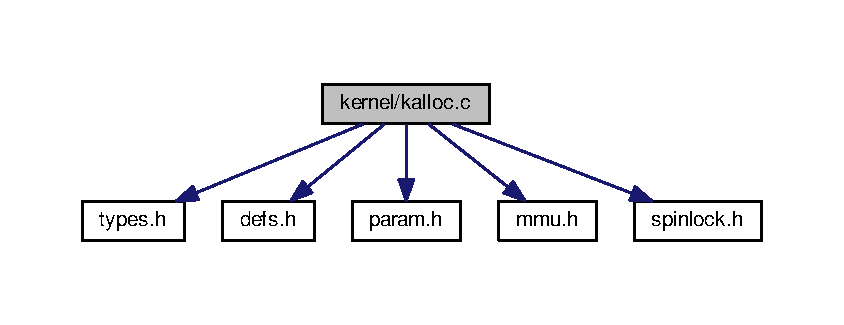
\includegraphics[width=350pt]{kalloc_8c__incl}
\end{center}
\end{figure}
\subsection*{Data Structures}
\begin{DoxyCompactItemize}
\item 
struct \hyperlink{structrun}{run}
\end{DoxyCompactItemize}
\subsection*{Functions}
\begin{DoxyCompactItemize}
\item 
void \hyperlink{kalloc_8c_a71d803d14f0e1b0682e2c20e7c2a7f7a}{kinit} (void)
\item 
void \hyperlink{kalloc_8c_aced59ecf8411235f6dffc065236711a5}{kfree} (char $\ast$v)
\item 
char $\ast$ \hyperlink{kalloc_8c_a3af104ba40b66dcec8363ac5a70907ed}{kalloc} (void)
\end{DoxyCompactItemize}
\subsection*{Variables}
\begin{DoxyCompactItemize}
\item 
\begin{tabbing}
xx\=xx\=xx\=xx\=xx\=xx\=xx\=xx\=xx\=\kill
struct \{\\
\>struct \hyperlink{structspinlock}{spinlock} \hyperlink{kalloc_8c_ab28e82cd5dda7d960095706a3ea20572}{lock}\\
\>struct \hyperlink{structrun}{run} $\ast$ \hyperlink{kalloc_8c_a25f1f0e27ad1cafebbde0b8b7455afb4}{freelist}\\
\} \hyperlink{kalloc_8c_a2954ba14fcdb793e2e0ca451af37607f}{kmem}\\

\end{tabbing}\item 
char \hyperlink{kalloc_8c_af4f810c521bcfd87215d3007005a8325}{end} \mbox{[}$\,$\mbox{]}
\end{DoxyCompactItemize}


\subsection{Function Documentation}
\hypertarget{kalloc_8c_a3af104ba40b66dcec8363ac5a70907ed}{\index{kalloc.\-c@{kalloc.\-c}!kalloc@{kalloc}}
\index{kalloc@{kalloc}!kalloc.c@{kalloc.\-c}}
\subsubsection[{kalloc}]{\setlength{\rightskip}{0pt plus 5cm}char$\ast$ kalloc (
\begin{DoxyParamCaption}
\item[{void}]{}
\end{DoxyParamCaption}
)}}\label{kalloc_8c_a3af104ba40b66dcec8363ac5a70907ed}


Definition at line 60 of file kalloc.\-c.

\hypertarget{kalloc_8c_aced59ecf8411235f6dffc065236711a5}{\index{kalloc.\-c@{kalloc.\-c}!kfree@{kfree}}
\index{kfree@{kfree}!kalloc.c@{kalloc.\-c}}
\subsubsection[{kfree}]{\setlength{\rightskip}{0pt plus 5cm}void kfree (
\begin{DoxyParamCaption}
\item[{char $\ast$}]{v}
\end{DoxyParamCaption}
)}}\label{kalloc_8c_aced59ecf8411235f6dffc065236711a5}


Definition at line 39 of file kalloc.\-c.

\hypertarget{kalloc_8c_a71d803d14f0e1b0682e2c20e7c2a7f7a}{\index{kalloc.\-c@{kalloc.\-c}!kinit@{kinit}}
\index{kinit@{kinit}!kalloc.c@{kalloc.\-c}}
\subsubsection[{kinit}]{\setlength{\rightskip}{0pt plus 5cm}void kinit (
\begin{DoxyParamCaption}
\item[{void}]{}
\end{DoxyParamCaption}
)}}\label{kalloc_8c_a71d803d14f0e1b0682e2c20e7c2a7f7a}


Definition at line 24 of file kalloc.\-c.



\subsection{Variable Documentation}
\hypertarget{kalloc_8c_af4f810c521bcfd87215d3007005a8325}{\index{kalloc.\-c@{kalloc.\-c}!end@{end}}
\index{end@{end}!kalloc.c@{kalloc.\-c}}
\subsubsection[{end}]{\setlength{\rightskip}{0pt plus 5cm}char end\mbox{[}$\,$\mbox{]}}}\label{kalloc_8c_af4f810c521bcfd87215d3007005a8325}
\hypertarget{kalloc_8c_a25f1f0e27ad1cafebbde0b8b7455afb4}{\index{kalloc.\-c@{kalloc.\-c}!freelist@{freelist}}
\index{freelist@{freelist}!kalloc.c@{kalloc.\-c}}
\subsubsection[{freelist}]{\setlength{\rightskip}{0pt plus 5cm}struct {\bf run}$\ast$ freelist}}\label{kalloc_8c_a25f1f0e27ad1cafebbde0b8b7455afb4}


Definition at line 17 of file kalloc.\-c.

\hypertarget{kalloc_8c_a2954ba14fcdb793e2e0ca451af37607f}{\index{kalloc.\-c@{kalloc.\-c}!kmem@{kmem}}
\index{kmem@{kmem}!kalloc.c@{kalloc.\-c}}
\subsubsection[{kmem}]{\setlength{\rightskip}{0pt plus 5cm}struct \{ ... \}   kmem}}\label{kalloc_8c_a2954ba14fcdb793e2e0ca451af37607f}
\hypertarget{kalloc_8c_ab28e82cd5dda7d960095706a3ea20572}{\index{kalloc.\-c@{kalloc.\-c}!lock@{lock}}
\index{lock@{lock}!kalloc.c@{kalloc.\-c}}
\subsubsection[{lock}]{\setlength{\rightskip}{0pt plus 5cm}struct {\bf spinlock} lock}}\label{kalloc_8c_ab28e82cd5dda7d960095706a3ea20572}


Definition at line 16 of file kalloc.\-c.


\hypertarget{kalloc_8d}{\section{kernel/kalloc.d File Reference}
\label{kalloc_8d}\index{kernel/kalloc.\-d@{kernel/kalloc.\-d}}
}

\hypertarget{kbd_8c}{\section{kernel/kbd.c File Reference}
\label{kbd_8c}\index{kernel/kbd.\-c@{kernel/kbd.\-c}}
}
{\ttfamily \#include \char`\"{}types.\-h\char`\"{}}\\*
{\ttfamily \#include \char`\"{}x86.\-h\char`\"{}}\\*
{\ttfamily \#include \char`\"{}defs.\-h\char`\"{}}\\*
{\ttfamily \#include \char`\"{}kbd.\-h\char`\"{}}\\*
Include dependency graph for kbd.\-c\-:
\nopagebreak
\begin{figure}[H]
\begin{center}
\leavevmode
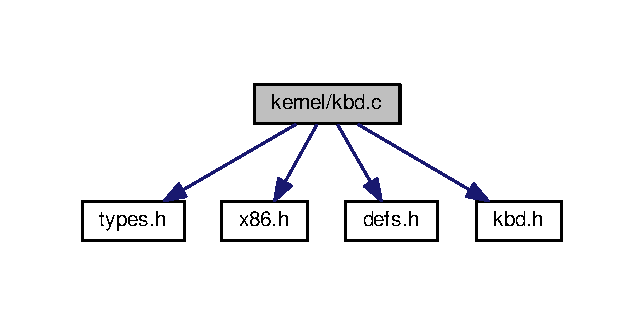
\includegraphics[width=309pt]{kbd_8c__incl}
\end{center}
\end{figure}
\subsection*{Functions}
\begin{DoxyCompactItemize}
\item 
int \hyperlink{kbd_8c_ae0e5224d52563340db794138daec14ca}{kbdgetc} (void)
\item 
void \hyperlink{kbd_8c_af3d6113fa152781400e1e0e728c55e54}{kbdintr} (void)
\end{DoxyCompactItemize}


\subsection{Function Documentation}
\hypertarget{kbd_8c_ae0e5224d52563340db794138daec14ca}{\index{kbd.\-c@{kbd.\-c}!kbdgetc@{kbdgetc}}
\index{kbdgetc@{kbdgetc}!kbd.c@{kbd.\-c}}
\subsubsection[{kbdgetc}]{\setlength{\rightskip}{0pt plus 5cm}int kbdgetc (
\begin{DoxyParamCaption}
\item[{void}]{}
\end{DoxyParamCaption}
)}}\label{kbd_8c_ae0e5224d52563340db794138daec14ca}


Definition at line 7 of file kbd.\-c.

\hypertarget{kbd_8c_af3d6113fa152781400e1e0e728c55e54}{\index{kbd.\-c@{kbd.\-c}!kbdintr@{kbdintr}}
\index{kbdintr@{kbdintr}!kbd.c@{kbd.\-c}}
\subsubsection[{kbdintr}]{\setlength{\rightskip}{0pt plus 5cm}void kbdintr (
\begin{DoxyParamCaption}
\item[{void}]{}
\end{DoxyParamCaption}
)}}\label{kbd_8c_af3d6113fa152781400e1e0e728c55e54}


Definition at line 47 of file kbd.\-c.


\hypertarget{kbd_8d}{\section{kernel/kbd.d File Reference}
\label{kbd_8d}\index{kernel/kbd.\-d@{kernel/kbd.\-d}}
}

\hypertarget{kbd_8h}{\section{kernel/kbd.h File Reference}
\label{kbd_8h}\index{kernel/kbd.\-h@{kernel/kbd.\-h}}
}
This graph shows which files directly or indirectly include this file\-:
\nopagebreak
\begin{figure}[H]
\begin{center}
\leavevmode
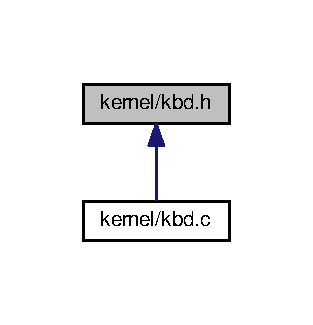
\includegraphics[width=150pt]{kbd_8h__dep__incl}
\end{center}
\end{figure}
\subsection*{Macros}
\begin{DoxyCompactItemize}
\item 
\#define \hyperlink{kbd_8h_a1e08ef54d0e877b370fbcc693b3e5aec}{K\-B\-S\-T\-A\-T\-P}~0x64
\item 
\#define \hyperlink{kbd_8h_a18012677006211070f49c39e758c1e18}{K\-B\-S\-\_\-\-D\-I\-B}~0x01
\item 
\#define \hyperlink{kbd_8h_ae4a1cdd6f51065e61bc7e61b491ab508}{K\-B\-D\-A\-T\-A\-P}~0x60
\item 
\#define \hyperlink{kbd_8h_a996bde01ecac342918f0a2c4e7ce7bd5}{N\-O}~0
\item 
\#define \hyperlink{kbd_8h_ac179eef68bcc694aa0ef8dd1eb09950b}{S\-H\-I\-F\-T}~(1$<$$<$0)
\item 
\#define \hyperlink{kbd_8h_ac16e9c5c93955f2c396aaa9829b72323}{C\-T\-L}~(1$<$$<$1)
\item 
\#define \hyperlink{kbd_8h_a9d8a33b1a8b82b9913a0ba70438d45be}{A\-L\-T}~(1$<$$<$2)
\item 
\#define \hyperlink{kbd_8h_ad36c01c5d7b1fc13a22426a497ac1b8b}{C\-A\-P\-S\-L\-O\-C\-K}~(1$<$$<$3)
\item 
\#define \hyperlink{kbd_8h_a67aa85b3ef56be57b97e084f52621d4f}{N\-U\-M\-L\-O\-C\-K}~(1$<$$<$4)
\item 
\#define \hyperlink{kbd_8h_a1cb9c7b41422a2c83136cecfe2a059d3}{S\-C\-R\-O\-L\-L\-L\-O\-C\-K}~(1$<$$<$5)
\item 
\#define \hyperlink{kbd_8h_a888d30b7a32808c7cdf95bfa59bf13b4}{E0\-E\-S\-C}~(1$<$$<$6)
\item 
\#define \hyperlink{kbd_8h_af6806366178266b3eaf1fb16f991cbee}{K\-E\-Y\-\_\-\-H\-O\-M\-E}~0x\-E0
\item 
\#define \hyperlink{kbd_8h_a912861b945e779c29f718cdcd62be10c}{K\-E\-Y\-\_\-\-E\-N\-D}~0x\-E1
\item 
\#define \hyperlink{kbd_8h_afa086fc916a81e7fd348ec00cf786916}{K\-E\-Y\-\_\-\-U\-P}~0x\-E2
\item 
\#define \hyperlink{kbd_8h_a69aff5c97fd814c5f29fca79bdcda9be}{K\-E\-Y\-\_\-\-D\-N}~0x\-E3
\item 
\#define \hyperlink{kbd_8h_afe0182b9752acbeff23e5b01e63ffe9c}{K\-E\-Y\-\_\-\-L\-F}~0x\-E4
\item 
\#define \hyperlink{kbd_8h_ab787b56ca072749c919b02381f66d271}{K\-E\-Y\-\_\-\-R\-T}~0x\-E5
\item 
\#define \hyperlink{kbd_8h_ac35c65d4a20c05b2cc7e1f3e40e13e79}{K\-E\-Y\-\_\-\-P\-G\-U\-P}~0x\-E6
\item 
\#define \hyperlink{kbd_8h_a84a56bcd66075dce29dd77873006f33c}{K\-E\-Y\-\_\-\-P\-G\-D\-N}~0x\-E7
\item 
\#define \hyperlink{kbd_8h_a4ea8f40f4220377b764d1b3b14807f2b}{K\-E\-Y\-\_\-\-I\-N\-S}~0x\-E8
\item 
\#define \hyperlink{kbd_8h_ad06e66a899b065c65c2363233d8ebce2}{K\-E\-Y\-\_\-\-D\-E\-L}~0x\-E9
\item 
\#define \hyperlink{kbd_8h_ac54ae397901fe700628cafadea3c5208}{C}(x)~(x -\/ '@')
\end{DoxyCompactItemize}


\subsection{Macro Definition Documentation}
\hypertarget{kbd_8h_a9d8a33b1a8b82b9913a0ba70438d45be}{\index{kbd.\-h@{kbd.\-h}!A\-L\-T@{A\-L\-T}}
\index{A\-L\-T@{A\-L\-T}!kbd.h@{kbd.\-h}}
\subsubsection[{A\-L\-T}]{\setlength{\rightskip}{0pt plus 5cm}\#define A\-L\-T~(1$<$$<$2)}}\label{kbd_8h_a9d8a33b1a8b82b9913a0ba70438d45be}


Definition at line 13 of file kbd.\-h.

\hypertarget{kbd_8h_ac54ae397901fe700628cafadea3c5208}{\index{kbd.\-h@{kbd.\-h}!C@{C}}
\index{C@{C}!kbd.h@{kbd.\-h}}
\subsubsection[{C}]{\setlength{\rightskip}{0pt plus 5cm}\#define C(
\begin{DoxyParamCaption}
\item[{}]{x}
\end{DoxyParamCaption}
)~(x -\/ '@')}}\label{kbd_8h_ac54ae397901fe700628cafadea3c5208}


Definition at line 34 of file kbd.\-h.

\hypertarget{kbd_8h_ad36c01c5d7b1fc13a22426a497ac1b8b}{\index{kbd.\-h@{kbd.\-h}!C\-A\-P\-S\-L\-O\-C\-K@{C\-A\-P\-S\-L\-O\-C\-K}}
\index{C\-A\-P\-S\-L\-O\-C\-K@{C\-A\-P\-S\-L\-O\-C\-K}!kbd.h@{kbd.\-h}}
\subsubsection[{C\-A\-P\-S\-L\-O\-C\-K}]{\setlength{\rightskip}{0pt plus 5cm}\#define C\-A\-P\-S\-L\-O\-C\-K~(1$<$$<$3)}}\label{kbd_8h_ad36c01c5d7b1fc13a22426a497ac1b8b}


Definition at line 15 of file kbd.\-h.

\hypertarget{kbd_8h_ac16e9c5c93955f2c396aaa9829b72323}{\index{kbd.\-h@{kbd.\-h}!C\-T\-L@{C\-T\-L}}
\index{C\-T\-L@{C\-T\-L}!kbd.h@{kbd.\-h}}
\subsubsection[{C\-T\-L}]{\setlength{\rightskip}{0pt plus 5cm}\#define C\-T\-L~(1$<$$<$1)}}\label{kbd_8h_ac16e9c5c93955f2c396aaa9829b72323}


Definition at line 12 of file kbd.\-h.

\hypertarget{kbd_8h_a888d30b7a32808c7cdf95bfa59bf13b4}{\index{kbd.\-h@{kbd.\-h}!E0\-E\-S\-C@{E0\-E\-S\-C}}
\index{E0\-E\-S\-C@{E0\-E\-S\-C}!kbd.h@{kbd.\-h}}
\subsubsection[{E0\-E\-S\-C}]{\setlength{\rightskip}{0pt plus 5cm}\#define E0\-E\-S\-C~(1$<$$<$6)}}\label{kbd_8h_a888d30b7a32808c7cdf95bfa59bf13b4}


Definition at line 19 of file kbd.\-h.

\hypertarget{kbd_8h_ae4a1cdd6f51065e61bc7e61b491ab508}{\index{kbd.\-h@{kbd.\-h}!K\-B\-D\-A\-T\-A\-P@{K\-B\-D\-A\-T\-A\-P}}
\index{K\-B\-D\-A\-T\-A\-P@{K\-B\-D\-A\-T\-A\-P}!kbd.h@{kbd.\-h}}
\subsubsection[{K\-B\-D\-A\-T\-A\-P}]{\setlength{\rightskip}{0pt plus 5cm}\#define K\-B\-D\-A\-T\-A\-P~0x60}}\label{kbd_8h_ae4a1cdd6f51065e61bc7e61b491ab508}


Definition at line 7 of file kbd.\-h.

\hypertarget{kbd_8h_a18012677006211070f49c39e758c1e18}{\index{kbd.\-h@{kbd.\-h}!K\-B\-S\-\_\-\-D\-I\-B@{K\-B\-S\-\_\-\-D\-I\-B}}
\index{K\-B\-S\-\_\-\-D\-I\-B@{K\-B\-S\-\_\-\-D\-I\-B}!kbd.h@{kbd.\-h}}
\subsubsection[{K\-B\-S\-\_\-\-D\-I\-B}]{\setlength{\rightskip}{0pt plus 5cm}\#define K\-B\-S\-\_\-\-D\-I\-B~0x01}}\label{kbd_8h_a18012677006211070f49c39e758c1e18}


Definition at line 6 of file kbd.\-h.

\hypertarget{kbd_8h_a1e08ef54d0e877b370fbcc693b3e5aec}{\index{kbd.\-h@{kbd.\-h}!K\-B\-S\-T\-A\-T\-P@{K\-B\-S\-T\-A\-T\-P}}
\index{K\-B\-S\-T\-A\-T\-P@{K\-B\-S\-T\-A\-T\-P}!kbd.h@{kbd.\-h}}
\subsubsection[{K\-B\-S\-T\-A\-T\-P}]{\setlength{\rightskip}{0pt plus 5cm}\#define K\-B\-S\-T\-A\-T\-P~0x64}}\label{kbd_8h_a1e08ef54d0e877b370fbcc693b3e5aec}


Definition at line 5 of file kbd.\-h.

\hypertarget{kbd_8h_ad06e66a899b065c65c2363233d8ebce2}{\index{kbd.\-h@{kbd.\-h}!K\-E\-Y\-\_\-\-D\-E\-L@{K\-E\-Y\-\_\-\-D\-E\-L}}
\index{K\-E\-Y\-\_\-\-D\-E\-L@{K\-E\-Y\-\_\-\-D\-E\-L}!kbd.h@{kbd.\-h}}
\subsubsection[{K\-E\-Y\-\_\-\-D\-E\-L}]{\setlength{\rightskip}{0pt plus 5cm}\#define K\-E\-Y\-\_\-\-D\-E\-L~0x\-E9}}\label{kbd_8h_ad06e66a899b065c65c2363233d8ebce2}


Definition at line 31 of file kbd.\-h.

\hypertarget{kbd_8h_a69aff5c97fd814c5f29fca79bdcda9be}{\index{kbd.\-h@{kbd.\-h}!K\-E\-Y\-\_\-\-D\-N@{K\-E\-Y\-\_\-\-D\-N}}
\index{K\-E\-Y\-\_\-\-D\-N@{K\-E\-Y\-\_\-\-D\-N}!kbd.h@{kbd.\-h}}
\subsubsection[{K\-E\-Y\-\_\-\-D\-N}]{\setlength{\rightskip}{0pt plus 5cm}\#define K\-E\-Y\-\_\-\-D\-N~0x\-E3}}\label{kbd_8h_a69aff5c97fd814c5f29fca79bdcda9be}


Definition at line 25 of file kbd.\-h.

\hypertarget{kbd_8h_a912861b945e779c29f718cdcd62be10c}{\index{kbd.\-h@{kbd.\-h}!K\-E\-Y\-\_\-\-E\-N\-D@{K\-E\-Y\-\_\-\-E\-N\-D}}
\index{K\-E\-Y\-\_\-\-E\-N\-D@{K\-E\-Y\-\_\-\-E\-N\-D}!kbd.h@{kbd.\-h}}
\subsubsection[{K\-E\-Y\-\_\-\-E\-N\-D}]{\setlength{\rightskip}{0pt plus 5cm}\#define K\-E\-Y\-\_\-\-E\-N\-D~0x\-E1}}\label{kbd_8h_a912861b945e779c29f718cdcd62be10c}


Definition at line 23 of file kbd.\-h.

\hypertarget{kbd_8h_af6806366178266b3eaf1fb16f991cbee}{\index{kbd.\-h@{kbd.\-h}!K\-E\-Y\-\_\-\-H\-O\-M\-E@{K\-E\-Y\-\_\-\-H\-O\-M\-E}}
\index{K\-E\-Y\-\_\-\-H\-O\-M\-E@{K\-E\-Y\-\_\-\-H\-O\-M\-E}!kbd.h@{kbd.\-h}}
\subsubsection[{K\-E\-Y\-\_\-\-H\-O\-M\-E}]{\setlength{\rightskip}{0pt plus 5cm}\#define K\-E\-Y\-\_\-\-H\-O\-M\-E~0x\-E0}}\label{kbd_8h_af6806366178266b3eaf1fb16f991cbee}


Definition at line 22 of file kbd.\-h.

\hypertarget{kbd_8h_a4ea8f40f4220377b764d1b3b14807f2b}{\index{kbd.\-h@{kbd.\-h}!K\-E\-Y\-\_\-\-I\-N\-S@{K\-E\-Y\-\_\-\-I\-N\-S}}
\index{K\-E\-Y\-\_\-\-I\-N\-S@{K\-E\-Y\-\_\-\-I\-N\-S}!kbd.h@{kbd.\-h}}
\subsubsection[{K\-E\-Y\-\_\-\-I\-N\-S}]{\setlength{\rightskip}{0pt plus 5cm}\#define K\-E\-Y\-\_\-\-I\-N\-S~0x\-E8}}\label{kbd_8h_a4ea8f40f4220377b764d1b3b14807f2b}


Definition at line 30 of file kbd.\-h.

\hypertarget{kbd_8h_afe0182b9752acbeff23e5b01e63ffe9c}{\index{kbd.\-h@{kbd.\-h}!K\-E\-Y\-\_\-\-L\-F@{K\-E\-Y\-\_\-\-L\-F}}
\index{K\-E\-Y\-\_\-\-L\-F@{K\-E\-Y\-\_\-\-L\-F}!kbd.h@{kbd.\-h}}
\subsubsection[{K\-E\-Y\-\_\-\-L\-F}]{\setlength{\rightskip}{0pt plus 5cm}\#define K\-E\-Y\-\_\-\-L\-F~0x\-E4}}\label{kbd_8h_afe0182b9752acbeff23e5b01e63ffe9c}


Definition at line 26 of file kbd.\-h.

\hypertarget{kbd_8h_a84a56bcd66075dce29dd77873006f33c}{\index{kbd.\-h@{kbd.\-h}!K\-E\-Y\-\_\-\-P\-G\-D\-N@{K\-E\-Y\-\_\-\-P\-G\-D\-N}}
\index{K\-E\-Y\-\_\-\-P\-G\-D\-N@{K\-E\-Y\-\_\-\-P\-G\-D\-N}!kbd.h@{kbd.\-h}}
\subsubsection[{K\-E\-Y\-\_\-\-P\-G\-D\-N}]{\setlength{\rightskip}{0pt plus 5cm}\#define K\-E\-Y\-\_\-\-P\-G\-D\-N~0x\-E7}}\label{kbd_8h_a84a56bcd66075dce29dd77873006f33c}


Definition at line 29 of file kbd.\-h.

\hypertarget{kbd_8h_ac35c65d4a20c05b2cc7e1f3e40e13e79}{\index{kbd.\-h@{kbd.\-h}!K\-E\-Y\-\_\-\-P\-G\-U\-P@{K\-E\-Y\-\_\-\-P\-G\-U\-P}}
\index{K\-E\-Y\-\_\-\-P\-G\-U\-P@{K\-E\-Y\-\_\-\-P\-G\-U\-P}!kbd.h@{kbd.\-h}}
\subsubsection[{K\-E\-Y\-\_\-\-P\-G\-U\-P}]{\setlength{\rightskip}{0pt plus 5cm}\#define K\-E\-Y\-\_\-\-P\-G\-U\-P~0x\-E6}}\label{kbd_8h_ac35c65d4a20c05b2cc7e1f3e40e13e79}


Definition at line 28 of file kbd.\-h.

\hypertarget{kbd_8h_ab787b56ca072749c919b02381f66d271}{\index{kbd.\-h@{kbd.\-h}!K\-E\-Y\-\_\-\-R\-T@{K\-E\-Y\-\_\-\-R\-T}}
\index{K\-E\-Y\-\_\-\-R\-T@{K\-E\-Y\-\_\-\-R\-T}!kbd.h@{kbd.\-h}}
\subsubsection[{K\-E\-Y\-\_\-\-R\-T}]{\setlength{\rightskip}{0pt plus 5cm}\#define K\-E\-Y\-\_\-\-R\-T~0x\-E5}}\label{kbd_8h_ab787b56ca072749c919b02381f66d271}


Definition at line 27 of file kbd.\-h.

\hypertarget{kbd_8h_afa086fc916a81e7fd348ec00cf786916}{\index{kbd.\-h@{kbd.\-h}!K\-E\-Y\-\_\-\-U\-P@{K\-E\-Y\-\_\-\-U\-P}}
\index{K\-E\-Y\-\_\-\-U\-P@{K\-E\-Y\-\_\-\-U\-P}!kbd.h@{kbd.\-h}}
\subsubsection[{K\-E\-Y\-\_\-\-U\-P}]{\setlength{\rightskip}{0pt plus 5cm}\#define K\-E\-Y\-\_\-\-U\-P~0x\-E2}}\label{kbd_8h_afa086fc916a81e7fd348ec00cf786916}


Definition at line 24 of file kbd.\-h.

\hypertarget{kbd_8h_a996bde01ecac342918f0a2c4e7ce7bd5}{\index{kbd.\-h@{kbd.\-h}!N\-O@{N\-O}}
\index{N\-O@{N\-O}!kbd.h@{kbd.\-h}}
\subsubsection[{N\-O}]{\setlength{\rightskip}{0pt plus 5cm}\#define N\-O~0}}\label{kbd_8h_a996bde01ecac342918f0a2c4e7ce7bd5}


Definition at line 9 of file kbd.\-h.

\hypertarget{kbd_8h_a67aa85b3ef56be57b97e084f52621d4f}{\index{kbd.\-h@{kbd.\-h}!N\-U\-M\-L\-O\-C\-K@{N\-U\-M\-L\-O\-C\-K}}
\index{N\-U\-M\-L\-O\-C\-K@{N\-U\-M\-L\-O\-C\-K}!kbd.h@{kbd.\-h}}
\subsubsection[{N\-U\-M\-L\-O\-C\-K}]{\setlength{\rightskip}{0pt plus 5cm}\#define N\-U\-M\-L\-O\-C\-K~(1$<$$<$4)}}\label{kbd_8h_a67aa85b3ef56be57b97e084f52621d4f}


Definition at line 16 of file kbd.\-h.

\hypertarget{kbd_8h_a1cb9c7b41422a2c83136cecfe2a059d3}{\index{kbd.\-h@{kbd.\-h}!S\-C\-R\-O\-L\-L\-L\-O\-C\-K@{S\-C\-R\-O\-L\-L\-L\-O\-C\-K}}
\index{S\-C\-R\-O\-L\-L\-L\-O\-C\-K@{S\-C\-R\-O\-L\-L\-L\-O\-C\-K}!kbd.h@{kbd.\-h}}
\subsubsection[{S\-C\-R\-O\-L\-L\-L\-O\-C\-K}]{\setlength{\rightskip}{0pt plus 5cm}\#define S\-C\-R\-O\-L\-L\-L\-O\-C\-K~(1$<$$<$5)}}\label{kbd_8h_a1cb9c7b41422a2c83136cecfe2a059d3}


Definition at line 17 of file kbd.\-h.

\hypertarget{kbd_8h_ac179eef68bcc694aa0ef8dd1eb09950b}{\index{kbd.\-h@{kbd.\-h}!S\-H\-I\-F\-T@{S\-H\-I\-F\-T}}
\index{S\-H\-I\-F\-T@{S\-H\-I\-F\-T}!kbd.h@{kbd.\-h}}
\subsubsection[{S\-H\-I\-F\-T}]{\setlength{\rightskip}{0pt plus 5cm}\#define S\-H\-I\-F\-T~(1$<$$<$0)}}\label{kbd_8h_ac179eef68bcc694aa0ef8dd1eb09950b}


Definition at line 11 of file kbd.\-h.


\hypertarget{lapic_8c}{\section{kernel/lapic.c File Reference}
\label{lapic_8c}\index{kernel/lapic.\-c@{kernel/lapic.\-c}}
}
{\ttfamily \#include \char`\"{}types.\-h\char`\"{}}\\*
{\ttfamily \#include \char`\"{}defs.\-h\char`\"{}}\\*
{\ttfamily \#include \char`\"{}traps.\-h\char`\"{}}\\*
{\ttfamily \#include \char`\"{}mmu.\-h\char`\"{}}\\*
{\ttfamily \#include \char`\"{}x86.\-h\char`\"{}}\\*
Include dependency graph for lapic.\-c\-:
\nopagebreak
\begin{figure}[H]
\begin{center}
\leavevmode
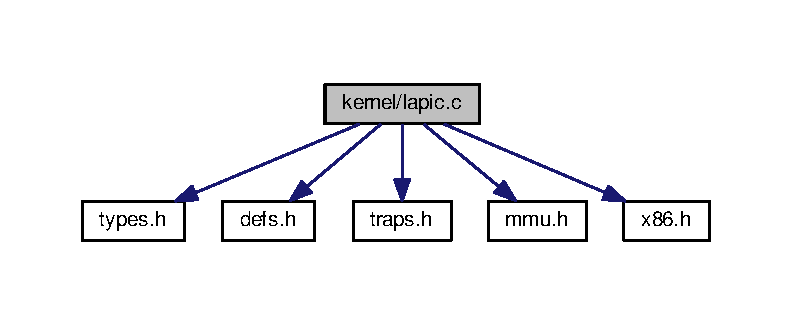
\includegraphics[width=350pt]{lapic_8c__incl}
\end{center}
\end{figure}
\subsection*{Macros}
\begin{DoxyCompactItemize}
\item 
\#define \hyperlink{lapic_8c_a77ceac8d6af195fe72f95f6afd87c45e}{I\-D}~(0x0020/4)
\item 
\#define \hyperlink{lapic_8c_a98ed931f97fef7e06e3ea441d0326c67}{V\-E\-R}~(0x0030/4)
\item 
\#define \hyperlink{lapic_8c_a0d378efcaaff1100c96bff8856bfc036}{T\-P\-R}~(0x0080/4)
\item 
\#define \hyperlink{lapic_8c_a04c9015da7e7ea45f3b80793809e2d7b}{E\-O\-I}~(0x00\-B0/4)
\item 
\#define \hyperlink{lapic_8c_a062fc16f4eacb723c76e2c87c8495412}{S\-V\-R}~(0x00\-F0/4)
\item 
\#define \hyperlink{lapic_8c_a514ad415fb6125ba296793df7d1a468a}{E\-N\-A\-B\-L\-E}~0x00000100
\item 
\#define \hyperlink{lapic_8c_ae4ad5e3805ffa2cbe03b65421edd8f99}{E\-S\-R}~(0x0280/4)
\item 
\#define \hyperlink{lapic_8c_ae6db3be23c343c0823604670010635f7}{I\-C\-R\-L\-O}~(0x0300/4)
\item 
\#define \hyperlink{lapic_8c_ab5889105dcd019008c9448dff61323f6}{I\-N\-I\-T}~0x00000500
\item 
\#define \hyperlink{lapic_8c_ad0dd8aa1d9d769cf15609ca108af4af9}{S\-T\-A\-R\-T\-U\-P}~0x00000600
\item 
\#define \hyperlink{lapic_8c_a5f0b856b460d14d6fac161e35cfdb9d1}{D\-E\-L\-I\-V\-S}~0x00001000
\item 
\#define \hyperlink{lapic_8c_af343b20373ba49a92fce523e948f2ab3}{A\-S\-S\-E\-R\-T}~0x00004000
\item 
\#define \hyperlink{lapic_8c_a8b48e10f84b81902cf66c89ac52649b7}{D\-E\-A\-S\-S\-E\-R\-T}~0x00000000
\item 
\#define \hyperlink{lapic_8c_a73f717b7aae31163c2a85f67883bf0ed}{L\-E\-V\-E\-L}~0x00008000
\item 
\#define \hyperlink{lapic_8c_adc4a14c073a7427003796cbd9d435758}{B\-C\-A\-S\-T}~0x00080000
\item 
\#define \hyperlink{lapic_8c_ab5be0aaddb58ffb9cb20c12530d66316}{B\-U\-S\-Y}~0x00001000
\item 
\#define \hyperlink{lapic_8c_a20207ffc8e6f0bdcefb5c42a5b5c3fb8}{F\-I\-X\-E\-D}~0x00000000
\item 
\#define \hyperlink{lapic_8c_a9382474befd66e12c502eb221e4f9a0d}{I\-C\-R\-H\-I}~(0x0310/4)
\item 
\#define \hyperlink{lapic_8c_a599217205dc3092c26567a2bd868ef3a}{T\-I\-M\-E\-R}~(0x0320/4)
\item 
\#define \hyperlink{lapic_8c_a1964818ccd90a6173ea48cecb652feeb}{X1}~0x0000000\-B
\item 
\#define \hyperlink{lapic_8c_af36821ad7b93ab31dcfaaa25e134fdf0}{P\-E\-R\-I\-O\-D\-I\-C}~0x00020000
\item 
\#define \hyperlink{lapic_8c_a5c989e3931132d4a4aca9cacfcb8b075}{P\-C\-I\-N\-T}~(0x0340/4)
\item 
\#define \hyperlink{lapic_8c_acec8cff36b5e5b2b4bda262480db2af2}{L\-I\-N\-T0}~(0x0350/4)
\item 
\#define \hyperlink{lapic_8c_a19035d504c49cf257ef4dc27cd3eb668}{L\-I\-N\-T1}~(0x0360/4)
\item 
\#define \hyperlink{lapic_8c_a8fe83ac76edc595f6b98cd4a4127aed5}{E\-R\-R\-O\-R}~(0x0370/4)
\item 
\#define \hyperlink{lapic_8c_a8fe9c058dcb81f528134d37e741182a3}{M\-A\-S\-K\-E\-D}~0x00010000
\item 
\#define \hyperlink{lapic_8c_af1d7a14061b402e4718eff6d9ef7ada4}{T\-I\-C\-R}~(0x0380/4)
\item 
\#define \hyperlink{lapic_8c_a1a73e99a3dd2d2d7dc6bbf084638e044}{T\-C\-C\-R}~(0x0390/4)
\item 
\#define \hyperlink{lapic_8c_a11b0b699f28c2043fcd6da289fff7375}{T\-D\-C\-R}~(0x03\-E0/4)
\item 
\#define \hyperlink{lapic_8c_a76c0053c859f3f56cf5cb1e2c5df5dd9}{I\-O\-\_\-\-R\-T\-C}~0x70
\end{DoxyCompactItemize}
\subsection*{Functions}
\begin{DoxyCompactItemize}
\item 
void \hyperlink{lapic_8c_abd5f53c2ab772d7cd392bf54122b3b9a}{lapicinit} (int c)
\item 
int \hyperlink{lapic_8c_ad07bc98847d46ba9772ab5ad4f52e6ec}{cpunum} (void)
\item 
void \hyperlink{lapic_8c_a42fdd0783bbeb7cdc646d360191cdcac}{lapiceoi} (void)
\item 
void \hyperlink{lapic_8c_ae0ac6441d1d76d8ef821cdbbc6b6fc2f}{microdelay} (int us)
\item 
void \hyperlink{lapic_8c_a54df00c792282426648d2876835958fa}{lapicstartap} (\hyperlink{types_8h_a65f85814a8290f9797005d3b28e7e5fc}{uchar} apicid, \hyperlink{types_8h_a91ad9478d81a7aaf2593e8d9c3d06a14}{uint} addr)
\end{DoxyCompactItemize}
\subsection*{Variables}
\begin{DoxyCompactItemize}
\item 
volatile \hyperlink{types_8h_a91ad9478d81a7aaf2593e8d9c3d06a14}{uint} $\ast$ \hyperlink{lapic_8c_a4029f3e2439d5912f93543b8addd10ec}{lapic}
\end{DoxyCompactItemize}


\subsection{Macro Definition Documentation}
\hypertarget{lapic_8c_af343b20373ba49a92fce523e948f2ab3}{\index{lapic.\-c@{lapic.\-c}!A\-S\-S\-E\-R\-T@{A\-S\-S\-E\-R\-T}}
\index{A\-S\-S\-E\-R\-T@{A\-S\-S\-E\-R\-T}!lapic.c@{lapic.\-c}}
\subsubsection[{A\-S\-S\-E\-R\-T}]{\setlength{\rightskip}{0pt plus 5cm}\#define A\-S\-S\-E\-R\-T~0x00004000}}\label{lapic_8c_af343b20373ba49a92fce523e948f2ab3}


Definition at line 22 of file lapic.\-c.

\hypertarget{lapic_8c_adc4a14c073a7427003796cbd9d435758}{\index{lapic.\-c@{lapic.\-c}!B\-C\-A\-S\-T@{B\-C\-A\-S\-T}}
\index{B\-C\-A\-S\-T@{B\-C\-A\-S\-T}!lapic.c@{lapic.\-c}}
\subsubsection[{B\-C\-A\-S\-T}]{\setlength{\rightskip}{0pt plus 5cm}\#define B\-C\-A\-S\-T~0x00080000}}\label{lapic_8c_adc4a14c073a7427003796cbd9d435758}


Definition at line 25 of file lapic.\-c.

\hypertarget{lapic_8c_ab5be0aaddb58ffb9cb20c12530d66316}{\index{lapic.\-c@{lapic.\-c}!B\-U\-S\-Y@{B\-U\-S\-Y}}
\index{B\-U\-S\-Y@{B\-U\-S\-Y}!lapic.c@{lapic.\-c}}
\subsubsection[{B\-U\-S\-Y}]{\setlength{\rightskip}{0pt plus 5cm}\#define B\-U\-S\-Y~0x00001000}}\label{lapic_8c_ab5be0aaddb58ffb9cb20c12530d66316}


Definition at line 26 of file lapic.\-c.

\hypertarget{lapic_8c_a8b48e10f84b81902cf66c89ac52649b7}{\index{lapic.\-c@{lapic.\-c}!D\-E\-A\-S\-S\-E\-R\-T@{D\-E\-A\-S\-S\-E\-R\-T}}
\index{D\-E\-A\-S\-S\-E\-R\-T@{D\-E\-A\-S\-S\-E\-R\-T}!lapic.c@{lapic.\-c}}
\subsubsection[{D\-E\-A\-S\-S\-E\-R\-T}]{\setlength{\rightskip}{0pt plus 5cm}\#define D\-E\-A\-S\-S\-E\-R\-T~0x00000000}}\label{lapic_8c_a8b48e10f84b81902cf66c89ac52649b7}


Definition at line 23 of file lapic.\-c.

\hypertarget{lapic_8c_a5f0b856b460d14d6fac161e35cfdb9d1}{\index{lapic.\-c@{lapic.\-c}!D\-E\-L\-I\-V\-S@{D\-E\-L\-I\-V\-S}}
\index{D\-E\-L\-I\-V\-S@{D\-E\-L\-I\-V\-S}!lapic.c@{lapic.\-c}}
\subsubsection[{D\-E\-L\-I\-V\-S}]{\setlength{\rightskip}{0pt plus 5cm}\#define D\-E\-L\-I\-V\-S~0x00001000}}\label{lapic_8c_a5f0b856b460d14d6fac161e35cfdb9d1}


Definition at line 21 of file lapic.\-c.

\hypertarget{lapic_8c_a514ad415fb6125ba296793df7d1a468a}{\index{lapic.\-c@{lapic.\-c}!E\-N\-A\-B\-L\-E@{E\-N\-A\-B\-L\-E}}
\index{E\-N\-A\-B\-L\-E@{E\-N\-A\-B\-L\-E}!lapic.c@{lapic.\-c}}
\subsubsection[{E\-N\-A\-B\-L\-E}]{\setlength{\rightskip}{0pt plus 5cm}\#define E\-N\-A\-B\-L\-E~0x00000100}}\label{lapic_8c_a514ad415fb6125ba296793df7d1a468a}


Definition at line 16 of file lapic.\-c.

\hypertarget{lapic_8c_a04c9015da7e7ea45f3b80793809e2d7b}{\index{lapic.\-c@{lapic.\-c}!E\-O\-I@{E\-O\-I}}
\index{E\-O\-I@{E\-O\-I}!lapic.c@{lapic.\-c}}
\subsubsection[{E\-O\-I}]{\setlength{\rightskip}{0pt plus 5cm}\#define E\-O\-I~(0x00\-B0/4)}}\label{lapic_8c_a04c9015da7e7ea45f3b80793809e2d7b}


Definition at line 14 of file lapic.\-c.

\hypertarget{lapic_8c_a8fe83ac76edc595f6b98cd4a4127aed5}{\index{lapic.\-c@{lapic.\-c}!E\-R\-R\-O\-R@{E\-R\-R\-O\-R}}
\index{E\-R\-R\-O\-R@{E\-R\-R\-O\-R}!lapic.c@{lapic.\-c}}
\subsubsection[{E\-R\-R\-O\-R}]{\setlength{\rightskip}{0pt plus 5cm}\#define E\-R\-R\-O\-R~(0x0370/4)}}\label{lapic_8c_a8fe83ac76edc595f6b98cd4a4127aed5}


Definition at line 35 of file lapic.\-c.

\hypertarget{lapic_8c_ae4ad5e3805ffa2cbe03b65421edd8f99}{\index{lapic.\-c@{lapic.\-c}!E\-S\-R@{E\-S\-R}}
\index{E\-S\-R@{E\-S\-R}!lapic.c@{lapic.\-c}}
\subsubsection[{E\-S\-R}]{\setlength{\rightskip}{0pt plus 5cm}\#define E\-S\-R~(0x0280/4)}}\label{lapic_8c_ae4ad5e3805ffa2cbe03b65421edd8f99}


Definition at line 17 of file lapic.\-c.

\hypertarget{lapic_8c_a20207ffc8e6f0bdcefb5c42a5b5c3fb8}{\index{lapic.\-c@{lapic.\-c}!F\-I\-X\-E\-D@{F\-I\-X\-E\-D}}
\index{F\-I\-X\-E\-D@{F\-I\-X\-E\-D}!lapic.c@{lapic.\-c}}
\subsubsection[{F\-I\-X\-E\-D}]{\setlength{\rightskip}{0pt plus 5cm}\#define F\-I\-X\-E\-D~0x00000000}}\label{lapic_8c_a20207ffc8e6f0bdcefb5c42a5b5c3fb8}


Definition at line 27 of file lapic.\-c.

\hypertarget{lapic_8c_a9382474befd66e12c502eb221e4f9a0d}{\index{lapic.\-c@{lapic.\-c}!I\-C\-R\-H\-I@{I\-C\-R\-H\-I}}
\index{I\-C\-R\-H\-I@{I\-C\-R\-H\-I}!lapic.c@{lapic.\-c}}
\subsubsection[{I\-C\-R\-H\-I}]{\setlength{\rightskip}{0pt plus 5cm}\#define I\-C\-R\-H\-I~(0x0310/4)}}\label{lapic_8c_a9382474befd66e12c502eb221e4f9a0d}


Definition at line 28 of file lapic.\-c.

\hypertarget{lapic_8c_ae6db3be23c343c0823604670010635f7}{\index{lapic.\-c@{lapic.\-c}!I\-C\-R\-L\-O@{I\-C\-R\-L\-O}}
\index{I\-C\-R\-L\-O@{I\-C\-R\-L\-O}!lapic.c@{lapic.\-c}}
\subsubsection[{I\-C\-R\-L\-O}]{\setlength{\rightskip}{0pt plus 5cm}\#define I\-C\-R\-L\-O~(0x0300/4)}}\label{lapic_8c_ae6db3be23c343c0823604670010635f7}


Definition at line 18 of file lapic.\-c.

\hypertarget{lapic_8c_a77ceac8d6af195fe72f95f6afd87c45e}{\index{lapic.\-c@{lapic.\-c}!I\-D@{I\-D}}
\index{I\-D@{I\-D}!lapic.c@{lapic.\-c}}
\subsubsection[{I\-D}]{\setlength{\rightskip}{0pt plus 5cm}\#define I\-D~(0x0020/4)}}\label{lapic_8c_a77ceac8d6af195fe72f95f6afd87c45e}


Definition at line 11 of file lapic.\-c.

\hypertarget{lapic_8c_ab5889105dcd019008c9448dff61323f6}{\index{lapic.\-c@{lapic.\-c}!I\-N\-I\-T@{I\-N\-I\-T}}
\index{I\-N\-I\-T@{I\-N\-I\-T}!lapic.c@{lapic.\-c}}
\subsubsection[{I\-N\-I\-T}]{\setlength{\rightskip}{0pt plus 5cm}\#define I\-N\-I\-T~0x00000500}}\label{lapic_8c_ab5889105dcd019008c9448dff61323f6}


Definition at line 19 of file lapic.\-c.

\hypertarget{lapic_8c_a76c0053c859f3f56cf5cb1e2c5df5dd9}{\index{lapic.\-c@{lapic.\-c}!I\-O\-\_\-\-R\-T\-C@{I\-O\-\_\-\-R\-T\-C}}
\index{I\-O\-\_\-\-R\-T\-C@{I\-O\-\_\-\-R\-T\-C}!lapic.c@{lapic.\-c}}
\subsubsection[{I\-O\-\_\-\-R\-T\-C}]{\setlength{\rightskip}{0pt plus 5cm}\#define I\-O\-\_\-\-R\-T\-C~0x70}}\label{lapic_8c_a76c0053c859f3f56cf5cb1e2c5df5dd9}


Definition at line 132 of file lapic.\-c.

\hypertarget{lapic_8c_a73f717b7aae31163c2a85f67883bf0ed}{\index{lapic.\-c@{lapic.\-c}!L\-E\-V\-E\-L@{L\-E\-V\-E\-L}}
\index{L\-E\-V\-E\-L@{L\-E\-V\-E\-L}!lapic.c@{lapic.\-c}}
\subsubsection[{L\-E\-V\-E\-L}]{\setlength{\rightskip}{0pt plus 5cm}\#define L\-E\-V\-E\-L~0x00008000}}\label{lapic_8c_a73f717b7aae31163c2a85f67883bf0ed}


Definition at line 24 of file lapic.\-c.

\hypertarget{lapic_8c_acec8cff36b5e5b2b4bda262480db2af2}{\index{lapic.\-c@{lapic.\-c}!L\-I\-N\-T0@{L\-I\-N\-T0}}
\index{L\-I\-N\-T0@{L\-I\-N\-T0}!lapic.c@{lapic.\-c}}
\subsubsection[{L\-I\-N\-T0}]{\setlength{\rightskip}{0pt plus 5cm}\#define L\-I\-N\-T0~(0x0350/4)}}\label{lapic_8c_acec8cff36b5e5b2b4bda262480db2af2}


Definition at line 33 of file lapic.\-c.

\hypertarget{lapic_8c_a19035d504c49cf257ef4dc27cd3eb668}{\index{lapic.\-c@{lapic.\-c}!L\-I\-N\-T1@{L\-I\-N\-T1}}
\index{L\-I\-N\-T1@{L\-I\-N\-T1}!lapic.c@{lapic.\-c}}
\subsubsection[{L\-I\-N\-T1}]{\setlength{\rightskip}{0pt plus 5cm}\#define L\-I\-N\-T1~(0x0360/4)}}\label{lapic_8c_a19035d504c49cf257ef4dc27cd3eb668}


Definition at line 34 of file lapic.\-c.

\hypertarget{lapic_8c_a8fe9c058dcb81f528134d37e741182a3}{\index{lapic.\-c@{lapic.\-c}!M\-A\-S\-K\-E\-D@{M\-A\-S\-K\-E\-D}}
\index{M\-A\-S\-K\-E\-D@{M\-A\-S\-K\-E\-D}!lapic.c@{lapic.\-c}}
\subsubsection[{M\-A\-S\-K\-E\-D}]{\setlength{\rightskip}{0pt plus 5cm}\#define M\-A\-S\-K\-E\-D~0x00010000}}\label{lapic_8c_a8fe9c058dcb81f528134d37e741182a3}


Definition at line 36 of file lapic.\-c.

\hypertarget{lapic_8c_a5c989e3931132d4a4aca9cacfcb8b075}{\index{lapic.\-c@{lapic.\-c}!P\-C\-I\-N\-T@{P\-C\-I\-N\-T}}
\index{P\-C\-I\-N\-T@{P\-C\-I\-N\-T}!lapic.c@{lapic.\-c}}
\subsubsection[{P\-C\-I\-N\-T}]{\setlength{\rightskip}{0pt plus 5cm}\#define P\-C\-I\-N\-T~(0x0340/4)}}\label{lapic_8c_a5c989e3931132d4a4aca9cacfcb8b075}


Definition at line 32 of file lapic.\-c.

\hypertarget{lapic_8c_af36821ad7b93ab31dcfaaa25e134fdf0}{\index{lapic.\-c@{lapic.\-c}!P\-E\-R\-I\-O\-D\-I\-C@{P\-E\-R\-I\-O\-D\-I\-C}}
\index{P\-E\-R\-I\-O\-D\-I\-C@{P\-E\-R\-I\-O\-D\-I\-C}!lapic.c@{lapic.\-c}}
\subsubsection[{P\-E\-R\-I\-O\-D\-I\-C}]{\setlength{\rightskip}{0pt plus 5cm}\#define P\-E\-R\-I\-O\-D\-I\-C~0x00020000}}\label{lapic_8c_af36821ad7b93ab31dcfaaa25e134fdf0}


Definition at line 31 of file lapic.\-c.

\hypertarget{lapic_8c_ad0dd8aa1d9d769cf15609ca108af4af9}{\index{lapic.\-c@{lapic.\-c}!S\-T\-A\-R\-T\-U\-P@{S\-T\-A\-R\-T\-U\-P}}
\index{S\-T\-A\-R\-T\-U\-P@{S\-T\-A\-R\-T\-U\-P}!lapic.c@{lapic.\-c}}
\subsubsection[{S\-T\-A\-R\-T\-U\-P}]{\setlength{\rightskip}{0pt plus 5cm}\#define S\-T\-A\-R\-T\-U\-P~0x00000600}}\label{lapic_8c_ad0dd8aa1d9d769cf15609ca108af4af9}


Definition at line 20 of file lapic.\-c.

\hypertarget{lapic_8c_a062fc16f4eacb723c76e2c87c8495412}{\index{lapic.\-c@{lapic.\-c}!S\-V\-R@{S\-V\-R}}
\index{S\-V\-R@{S\-V\-R}!lapic.c@{lapic.\-c}}
\subsubsection[{S\-V\-R}]{\setlength{\rightskip}{0pt plus 5cm}\#define S\-V\-R~(0x00\-F0/4)}}\label{lapic_8c_a062fc16f4eacb723c76e2c87c8495412}


Definition at line 15 of file lapic.\-c.

\hypertarget{lapic_8c_a1a73e99a3dd2d2d7dc6bbf084638e044}{\index{lapic.\-c@{lapic.\-c}!T\-C\-C\-R@{T\-C\-C\-R}}
\index{T\-C\-C\-R@{T\-C\-C\-R}!lapic.c@{lapic.\-c}}
\subsubsection[{T\-C\-C\-R}]{\setlength{\rightskip}{0pt plus 5cm}\#define T\-C\-C\-R~(0x0390/4)}}\label{lapic_8c_a1a73e99a3dd2d2d7dc6bbf084638e044}


Definition at line 38 of file lapic.\-c.

\hypertarget{lapic_8c_a11b0b699f28c2043fcd6da289fff7375}{\index{lapic.\-c@{lapic.\-c}!T\-D\-C\-R@{T\-D\-C\-R}}
\index{T\-D\-C\-R@{T\-D\-C\-R}!lapic.c@{lapic.\-c}}
\subsubsection[{T\-D\-C\-R}]{\setlength{\rightskip}{0pt plus 5cm}\#define T\-D\-C\-R~(0x03\-E0/4)}}\label{lapic_8c_a11b0b699f28c2043fcd6da289fff7375}


Definition at line 39 of file lapic.\-c.

\hypertarget{lapic_8c_af1d7a14061b402e4718eff6d9ef7ada4}{\index{lapic.\-c@{lapic.\-c}!T\-I\-C\-R@{T\-I\-C\-R}}
\index{T\-I\-C\-R@{T\-I\-C\-R}!lapic.c@{lapic.\-c}}
\subsubsection[{T\-I\-C\-R}]{\setlength{\rightskip}{0pt plus 5cm}\#define T\-I\-C\-R~(0x0380/4)}}\label{lapic_8c_af1d7a14061b402e4718eff6d9ef7ada4}


Definition at line 37 of file lapic.\-c.

\hypertarget{lapic_8c_a599217205dc3092c26567a2bd868ef3a}{\index{lapic.\-c@{lapic.\-c}!T\-I\-M\-E\-R@{T\-I\-M\-E\-R}}
\index{T\-I\-M\-E\-R@{T\-I\-M\-E\-R}!lapic.c@{lapic.\-c}}
\subsubsection[{T\-I\-M\-E\-R}]{\setlength{\rightskip}{0pt plus 5cm}\#define T\-I\-M\-E\-R~(0x0320/4)}}\label{lapic_8c_a599217205dc3092c26567a2bd868ef3a}


Definition at line 29 of file lapic.\-c.

\hypertarget{lapic_8c_a0d378efcaaff1100c96bff8856bfc036}{\index{lapic.\-c@{lapic.\-c}!T\-P\-R@{T\-P\-R}}
\index{T\-P\-R@{T\-P\-R}!lapic.c@{lapic.\-c}}
\subsubsection[{T\-P\-R}]{\setlength{\rightskip}{0pt plus 5cm}\#define T\-P\-R~(0x0080/4)}}\label{lapic_8c_a0d378efcaaff1100c96bff8856bfc036}


Definition at line 13 of file lapic.\-c.

\hypertarget{lapic_8c_a98ed931f97fef7e06e3ea441d0326c67}{\index{lapic.\-c@{lapic.\-c}!V\-E\-R@{V\-E\-R}}
\index{V\-E\-R@{V\-E\-R}!lapic.c@{lapic.\-c}}
\subsubsection[{V\-E\-R}]{\setlength{\rightskip}{0pt plus 5cm}\#define V\-E\-R~(0x0030/4)}}\label{lapic_8c_a98ed931f97fef7e06e3ea441d0326c67}


Definition at line 12 of file lapic.\-c.

\hypertarget{lapic_8c_a1964818ccd90a6173ea48cecb652feeb}{\index{lapic.\-c@{lapic.\-c}!X1@{X1}}
\index{X1@{X1}!lapic.c@{lapic.\-c}}
\subsubsection[{X1}]{\setlength{\rightskip}{0pt plus 5cm}\#define X1~0x0000000\-B}}\label{lapic_8c_a1964818ccd90a6173ea48cecb652feeb}


Definition at line 30 of file lapic.\-c.



\subsection{Function Documentation}
\hypertarget{lapic_8c_ad07bc98847d46ba9772ab5ad4f52e6ec}{\index{lapic.\-c@{lapic.\-c}!cpunum@{cpunum}}
\index{cpunum@{cpunum}!lapic.c@{lapic.\-c}}
\subsubsection[{cpunum}]{\setlength{\rightskip}{0pt plus 5cm}int cpunum (
\begin{DoxyParamCaption}
\item[{void}]{}
\end{DoxyParamCaption}
)}}\label{lapic_8c_ad07bc98847d46ba9772ab5ad4f52e6ec}


Definition at line 98 of file lapic.\-c.

\hypertarget{lapic_8c_a42fdd0783bbeb7cdc646d360191cdcac}{\index{lapic.\-c@{lapic.\-c}!lapiceoi@{lapiceoi}}
\index{lapiceoi@{lapiceoi}!lapic.c@{lapic.\-c}}
\subsubsection[{lapiceoi}]{\setlength{\rightskip}{0pt plus 5cm}void lapiceoi (
\begin{DoxyParamCaption}
\item[{void}]{}
\end{DoxyParamCaption}
)}}\label{lapic_8c_a42fdd0783bbeb7cdc646d360191cdcac}


Definition at line 119 of file lapic.\-c.

\hypertarget{lapic_8c_abd5f53c2ab772d7cd392bf54122b3b9a}{\index{lapic.\-c@{lapic.\-c}!lapicinit@{lapicinit}}
\index{lapicinit@{lapicinit}!lapic.c@{lapic.\-c}}
\subsubsection[{lapicinit}]{\setlength{\rightskip}{0pt plus 5cm}void lapicinit (
\begin{DoxyParamCaption}
\item[{int}]{c}
\end{DoxyParamCaption}
)}}\label{lapic_8c_abd5f53c2ab772d7cd392bf54122b3b9a}


Definition at line 51 of file lapic.\-c.

\hypertarget{lapic_8c_a54df00c792282426648d2876835958fa}{\index{lapic.\-c@{lapic.\-c}!lapicstartap@{lapicstartap}}
\index{lapicstartap@{lapicstartap}!lapic.c@{lapic.\-c}}
\subsubsection[{lapicstartap}]{\setlength{\rightskip}{0pt plus 5cm}void lapicstartap (
\begin{DoxyParamCaption}
\item[{{\bf uchar}}]{apicid, }
\item[{{\bf uint}}]{addr}
\end{DoxyParamCaption}
)}}\label{lapic_8c_a54df00c792282426648d2876835958fa}


Definition at line 137 of file lapic.\-c.

\hypertarget{lapic_8c_ae0ac6441d1d76d8ef821cdbbc6b6fc2f}{\index{lapic.\-c@{lapic.\-c}!microdelay@{microdelay}}
\index{microdelay@{microdelay}!lapic.c@{lapic.\-c}}
\subsubsection[{microdelay}]{\setlength{\rightskip}{0pt plus 5cm}void microdelay (
\begin{DoxyParamCaption}
\item[{int}]{us}
\end{DoxyParamCaption}
)}}\label{lapic_8c_ae0ac6441d1d76d8ef821cdbbc6b6fc2f}


Definition at line 128 of file lapic.\-c.



\subsection{Variable Documentation}
\hypertarget{lapic_8c_a4029f3e2439d5912f93543b8addd10ec}{\index{lapic.\-c@{lapic.\-c}!lapic@{lapic}}
\index{lapic@{lapic}!lapic.c@{lapic.\-c}}
\subsubsection[{lapic}]{\setlength{\rightskip}{0pt plus 5cm}volatile {\bf uint}$\ast$ lapic}}\label{lapic_8c_a4029f3e2439d5912f93543b8addd10ec}


Definition at line 41 of file lapic.\-c.


\hypertarget{lapic_8d}{\section{kernel/lapic.d File Reference}
\label{lapic_8d}\index{kernel/lapic.\-d@{kernel/lapic.\-d}}
}

\hypertarget{main_8c}{\section{kernel/main.c File Reference}
\label{main_8c}\index{kernel/main.\-c@{kernel/main.\-c}}
}
{\ttfamily \#include \char`\"{}types.\-h\char`\"{}}\\*
{\ttfamily \#include \char`\"{}defs.\-h\char`\"{}}\\*
{\ttfamily \#include \char`\"{}param.\-h\char`\"{}}\\*
{\ttfamily \#include \char`\"{}mmu.\-h\char`\"{}}\\*
{\ttfamily \#include \char`\"{}proc.\-h\char`\"{}}\\*
{\ttfamily \#include \char`\"{}x86.\-h\char`\"{}}\\*
Include dependency graph for main.\-c\-:
\nopagebreak
\begin{figure}[H]
\begin{center}
\leavevmode
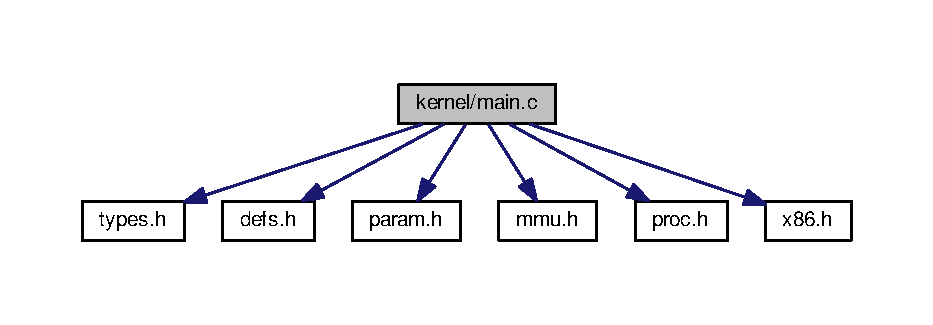
\includegraphics[width=350pt]{main_8c__incl}
\end{center}
\end{figure}
\subsection*{Functions}
\begin{DoxyCompactItemize}
\item 
void \hyperlink{main_8c_af3e715d75d66cf9f5df78656b5d2c87f}{jmpkstack} (void)
\item 
void \hyperlink{main_8c_a3a5428e8e62665a0567edb001a99a4be}{mainc} (void)
\end{DoxyCompactItemize}


\subsection{Function Documentation}
\hypertarget{main_8c_af3e715d75d66cf9f5df78656b5d2c87f}{\index{main.\-c@{main.\-c}!jmpkstack@{jmpkstack}}
\index{jmpkstack@{jmpkstack}!main.c@{main.\-c}}
\subsubsection[{jmpkstack}]{\setlength{\rightskip}{0pt plus 5cm}void jmpkstack (
\begin{DoxyParamCaption}
\item[{void}]{}
\end{DoxyParamCaption}
)}}\label{main_8c_af3e715d75d66cf9f5df78656b5d2c87f}


Definition at line 10 of file main.\-c.

\hypertarget{main_8c_a3a5428e8e62665a0567edb001a99a4be}{\index{main.\-c@{main.\-c}!mainc@{mainc}}
\index{mainc@{mainc}!main.c@{main.\-c}}
\subsubsection[{mainc}]{\setlength{\rightskip}{0pt plus 5cm}void mainc (
\begin{DoxyParamCaption}
\item[{void}]{}
\end{DoxyParamCaption}
)}}\label{main_8c_a3a5428e8e62665a0567edb001a99a4be}


Definition at line 43 of file main.\-c.


\hypertarget{main_8d}{\section{kernel/main.d File Reference}
\label{main_8d}\index{kernel/main.\-d@{kernel/main.\-d}}
}

\hypertarget{mmu_8h}{\section{kernel/mmu.h File Reference}
\label{mmu_8h}\index{kernel/mmu.\-h@{kernel/mmu.\-h}}
}
This graph shows which files directly or indirectly include this file\-:
\nopagebreak
\begin{figure}[H]
\begin{center}
\leavevmode
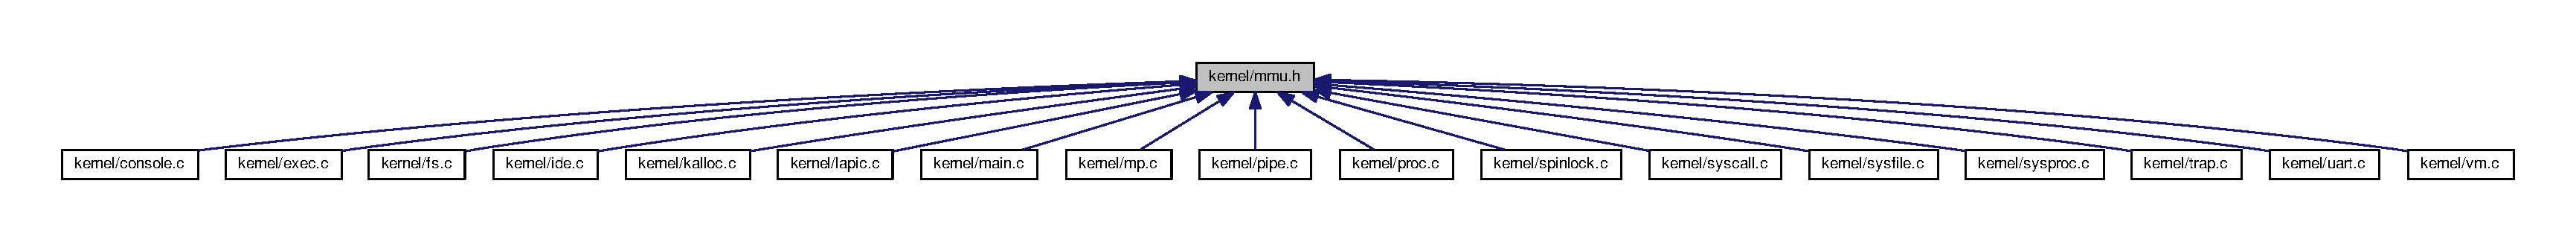
\includegraphics[width=350pt]{mmu_8h__dep__incl}
\end{center}
\end{figure}
\subsection*{Data Structures}
\begin{DoxyCompactItemize}
\item 
struct \hyperlink{structsegdesc}{segdesc}
\item 
struct \hyperlink{structtaskstate}{taskstate}
\item 
struct \hyperlink{structgatedesc}{gatedesc}
\end{DoxyCompactItemize}
\subsection*{Macros}
\begin{DoxyCompactItemize}
\item 
\#define \hyperlink{mmu_8h_a1d4cd77f3325c9f7f53fb7c0f5e49009}{F\-L\-\_\-\-C\-F}~0x00000001
\item 
\#define \hyperlink{mmu_8h_a1f1a4ea59207cc41d72dada6a4b0691c}{F\-L\-\_\-\-P\-F}~0x00000004
\item 
\#define \hyperlink{mmu_8h_a4927c16122d3d544048432ad6f90b689}{F\-L\-\_\-\-A\-F}~0x00000010
\item 
\#define \hyperlink{mmu_8h_a66e0b71057f84fa675ccc3bc22c73be9}{F\-L\-\_\-\-Z\-F}~0x00000040
\item 
\#define \hyperlink{mmu_8h_a6619f7a7aff26d04b23afcbc6660a58e}{F\-L\-\_\-\-S\-F}~0x00000080
\item 
\#define \hyperlink{mmu_8h_abd949387acf746559a2287f6e404235c}{F\-L\-\_\-\-T\-F}~0x00000100
\item 
\#define \hyperlink{mmu_8h_ab481068357bb42797aafe91864a2d085}{F\-L\-\_\-\-I\-F}~0x00000200
\item 
\#define \hyperlink{mmu_8h_afa5551d2e2438dc958983396a1f580d3}{F\-L\-\_\-\-D\-F}~0x00000400
\item 
\#define \hyperlink{mmu_8h_a94b53adb28e5c5d73f529569d58da643}{F\-L\-\_\-\-O\-F}~0x00000800
\item 
\#define \hyperlink{mmu_8h_a36ddfe6c6974596cd642138eee7dbe98}{F\-L\-\_\-\-I\-O\-P\-L\-\_\-\-M\-A\-S\-K}~0x00003000
\item 
\#define \hyperlink{mmu_8h_a3ed6d494edfe9cd89957726da3c20c2f}{F\-L\-\_\-\-I\-O\-P\-L\-\_\-0}~0x00000000
\item 
\#define \hyperlink{mmu_8h_acecae3043c790b6ed399d9a864c81595}{F\-L\-\_\-\-I\-O\-P\-L\-\_\-1}~0x00001000
\item 
\#define \hyperlink{mmu_8h_a4838447d144140d70f49776a3ca493de}{F\-L\-\_\-\-I\-O\-P\-L\-\_\-2}~0x00002000
\item 
\#define \hyperlink{mmu_8h_a65d57b1678c33e6c39cadb64457b36db}{F\-L\-\_\-\-I\-O\-P\-L\-\_\-3}~0x00003000
\item 
\#define \hyperlink{mmu_8h_ad5c3f2f9272df4c9d57a9487c4e1b50b}{F\-L\-\_\-\-N\-T}~0x00004000
\item 
\#define \hyperlink{mmu_8h_ade9786a06c1f327c37e1fe9ca3bc32b9}{F\-L\-\_\-\-R\-F}~0x00010000
\item 
\#define \hyperlink{mmu_8h_af7c82bf7715d78873a56ed04dfa9bd97}{F\-L\-\_\-\-V\-M}~0x00020000
\item 
\#define \hyperlink{mmu_8h_a9c71ec24fe8944c57bd3712b87644294}{F\-L\-\_\-\-A\-C}~0x00040000
\item 
\#define \hyperlink{mmu_8h_a5a8a6171bb4d6954ea080ebccf18fcf9}{F\-L\-\_\-\-V\-I\-F}~0x00080000
\item 
\#define \hyperlink{mmu_8h_ab5d8e8ca1f8cf4a7908f316435e25bb9}{F\-L\-\_\-\-V\-I\-P}~0x00100000
\item 
\#define \hyperlink{mmu_8h_a23f8f7b48086df377376e84d0bf65009}{F\-L\-\_\-\-I\-D}~0x00200000
\item 
\#define \hyperlink{mmu_8h_aa899fa0a2a7dd414343fb2fada767622}{C\-R0\-\_\-\-P\-E}~0x00000001
\item 
\#define \hyperlink{mmu_8h_a301019ca375756ccb75c7f207473e02d}{C\-R0\-\_\-\-M\-P}~0x00000002
\item 
\#define \hyperlink{mmu_8h_a39a8caf6348b3eae36171b43146025f6}{C\-R0\-\_\-\-E\-M}~0x00000004
\item 
\#define \hyperlink{mmu_8h_af9f6d1ac01fd24519da378e16b91b023}{C\-R0\-\_\-\-T\-S}~0x00000008
\item 
\#define \hyperlink{mmu_8h_ad13fdf98c38ada8515b3d490feba86e7}{C\-R0\-\_\-\-E\-T}~0x00000010
\item 
\#define \hyperlink{mmu_8h_a219c459acf834242afdd99cda9c6a42c}{C\-R0\-\_\-\-N\-E}~0x00000020
\item 
\#define \hyperlink{mmu_8h_a2897f244bf55b3cf87c13869db57f6c8}{C\-R0\-\_\-\-W\-P}~0x00010000
\item 
\#define \hyperlink{mmu_8h_a88b8c1f08a286fdaf7b58e10e4223771}{C\-R0\-\_\-\-A\-M}~0x00040000
\item 
\#define \hyperlink{mmu_8h_a0e3e94dacd9aafa4721822a934c10d9e}{C\-R0\-\_\-\-N\-W}~0x20000000
\item 
\#define \hyperlink{mmu_8h_ae2abb4033838584afd1413b3fcfe3e20}{C\-R0\-\_\-\-C\-D}~0x40000000
\item 
\#define \hyperlink{mmu_8h_a4f3b70ba40d96e55cae6026acc12cfed}{C\-R0\-\_\-\-P\-G}~0x80000000
\item 
\#define \hyperlink{mmu_8h_a1594ac4688d9f212e835fd38ff63e83f}{S\-E\-G}(type, base, lim, dpl)
\item 
\#define \hyperlink{mmu_8h_abe69a1dd6290e2be017d58309495adb7}{S\-E\-G16}(type, base, lim, dpl)
\item 
\#define \hyperlink{mmu_8h_a060d4d4e32af81cab881fe77e58d7b78}{D\-P\-L\-\_\-\-U\-S\-E\-R}~0x3
\item 
\#define \hyperlink{mmu_8h_af30c683a434e0712fd83781307239cb9}{S\-T\-A\-\_\-\-X}~0x8
\item 
\#define \hyperlink{mmu_8h_ad6f4adbc6fea020a7d9d18a5f709843e}{S\-T\-A\-\_\-\-E}~0x4
\item 
\#define \hyperlink{mmu_8h_ab4829c3150ed67ae0f00a103fb448a2f}{S\-T\-A\-\_\-\-C}~0x4
\item 
\#define \hyperlink{mmu_8h_a9321b5b232838b8b230c6b681be9a882}{S\-T\-A\-\_\-\-W}~0x2
\item 
\#define \hyperlink{mmu_8h_a6545a48f34a3fae1b04cf265f13bc8f3}{S\-T\-A\-\_\-\-R}~0x2
\item 
\#define \hyperlink{mmu_8h_a18eb795a2eb72794f4de5b8087731607}{S\-T\-A\-\_\-\-A}~0x1
\item 
\#define \hyperlink{mmu_8h_a92f6e9c3a88bc7b119e356214afb18d0}{S\-T\-S\-\_\-\-T16\-A}~0x1
\item 
\#define \hyperlink{mmu_8h_af82429cbe13d9fc970aa92082aa2b24f}{S\-T\-S\-\_\-\-L\-D\-T}~0x2
\item 
\#define \hyperlink{mmu_8h_a24f6ddb5ba92dab5a68f7f2cded0bb3a}{S\-T\-S\-\_\-\-T16\-B}~0x3
\item 
\#define \hyperlink{mmu_8h_a892428e720dfa978188d79cdd0380630}{S\-T\-S\-\_\-\-C\-G16}~0x4
\item 
\#define \hyperlink{mmu_8h_a52ec5ba90269a2040fc29d6a11e5c14c}{S\-T\-S\-\_\-\-T\-G}~0x5
\item 
\#define \hyperlink{mmu_8h_a8543847c09da13a951ab3009e49df956}{S\-T\-S\-\_\-\-I\-G16}~0x6
\item 
\#define \hyperlink{mmu_8h_a16d083797e265f35ef2a8edade986463}{S\-T\-S\-\_\-\-T\-G16}~0x7
\item 
\#define \hyperlink{mmu_8h_a1b27d53cef04c198f3b048345d28016c}{S\-T\-S\-\_\-\-T32\-A}~0x9
\item 
\#define \hyperlink{mmu_8h_af656e12a5bedfa79c0c3e02a3f01bab6}{S\-T\-S\-\_\-\-T32\-B}~0x\-B
\item 
\#define \hyperlink{mmu_8h_aa7e0b3f01699a15c5c49c54de3750107}{S\-T\-S\-\_\-\-C\-G32}~0x\-C
\item 
\#define \hyperlink{mmu_8h_a14b54d1a503921b0c10993cdc6ff197b}{S\-T\-S\-\_\-\-I\-G32}~0x\-E
\item 
\#define \hyperlink{mmu_8h_a734d7f1a24c70d7b410cf3a7cbe00093}{S\-T\-S\-\_\-\-T\-G32}~0x\-F
\item 
\#define \hyperlink{mmu_8h_a1b00ddfafd303030fd16bee16a42a2ce}{P\-D\-X}(la)~(((\hyperlink{types_8h_a91ad9478d81a7aaf2593e8d9c3d06a14}{uint})(la) $>$$>$ \hyperlink{mmu_8h_a6d2227e0acbc6e206494b5e50f0c5297}{P\-D\-X\-S\-H\-I\-F\-T}) \& 0x3\-F\-F)
\item 
\#define \hyperlink{mmu_8h_ac744451cc21b0b24f37dd8f0d51b43fc}{P\-T\-X}(la)~(((\hyperlink{types_8h_a91ad9478d81a7aaf2593e8d9c3d06a14}{uint})(la) $>$$>$ \hyperlink{mmu_8h_a4424facfb4be6b056c05ec638d6347de}{P\-T\-X\-S\-H\-I\-F\-T}) \& 0x3\-F\-F)
\item 
\#define \hyperlink{mmu_8h_a2e162e8ad6bc81877dd299db9fc87664}{P\-G\-A\-D\-D\-R}(d, t, o)~((\hyperlink{types_8h_a91ad9478d81a7aaf2593e8d9c3d06a14}{uint})((d) $<$$<$ \hyperlink{mmu_8h_a6d2227e0acbc6e206494b5e50f0c5297}{P\-D\-X\-S\-H\-I\-F\-T} $\vert$ (t) $<$$<$ \hyperlink{mmu_8h_a4424facfb4be6b056c05ec638d6347de}{P\-T\-X\-S\-H\-I\-F\-T} $\vert$ (o)))
\item 
\#define \hyperlink{mmu_8h_a3b7982928c5178b9244b2b6289ef3832}{P\-A\-D\-D\-R}(a)~((\hyperlink{types_8h_a91ad9478d81a7aaf2593e8d9c3d06a14}{uint})(a))
\item 
\#define \hyperlink{mmu_8h_af60ee3ecbf249497d0378c97201edfe8}{N\-P\-D\-E\-N\-T\-R\-I\-E\-S}~1024
\item 
\#define \hyperlink{mmu_8h_a6318b16289e829d7f9719134ba08704f}{N\-P\-T\-E\-N\-T\-R\-I\-E\-S}~1024
\item 
\#define \hyperlink{mmu_8h_a5f96cb6ae6670e023c407cc2f77e1704}{P\-G\-S\-I\-Z\-E}~4096
\item 
\#define \hyperlink{mmu_8h_a20d0b7c5f64f21a3fdc19cf44afe8ff2}{P\-G\-S\-H\-I\-F\-T}~12
\item 
\#define \hyperlink{mmu_8h_a4424facfb4be6b056c05ec638d6347de}{P\-T\-X\-S\-H\-I\-F\-T}~12
\item 
\#define \hyperlink{mmu_8h_a6d2227e0acbc6e206494b5e50f0c5297}{P\-D\-X\-S\-H\-I\-F\-T}~22
\item 
\#define \hyperlink{mmu_8h_affa8cdfbd1c15dafc9f3af3a7b641f80}{P\-G\-R\-O\-U\-N\-D\-U\-P}(sz)~(((sz)+\hyperlink{mmu_8h_a5f96cb6ae6670e023c407cc2f77e1704}{P\-G\-S\-I\-Z\-E}-\/1) \& $\sim$(\hyperlink{mmu_8h_a5f96cb6ae6670e023c407cc2f77e1704}{P\-G\-S\-I\-Z\-E}-\/1))
\item 
\#define \hyperlink{mmu_8h_a687e91750055553dd2788386c6a512fb}{P\-G\-R\-O\-U\-N\-D\-D\-O\-W\-N}(a)~((char$\ast$)((((unsigned int)(a)) \& $\sim$(\hyperlink{mmu_8h_a5f96cb6ae6670e023c407cc2f77e1704}{P\-G\-S\-I\-Z\-E}-\/1))))
\item 
\#define \hyperlink{mmu_8h_a89bd860de64c44cd8ebaca8dc311b5ac}{P\-T\-E\-\_\-\-P}~0x001
\item 
\#define \hyperlink{mmu_8h_a058fcbcc3e1eab2c09c68b3e5221c545}{P\-T\-E\-\_\-\-W}~0x002
\item 
\#define \hyperlink{mmu_8h_adced9836a1dc98d72849361e6ab03cda}{P\-T\-E\-\_\-\-U}~0x004
\item 
\#define \hyperlink{mmu_8h_a72dca8a3a88d5e77c35551286cc25f23}{P\-T\-E\-\_\-\-P\-W\-T}~0x008
\item 
\#define \hyperlink{mmu_8h_a120b9b6cd80216401185944eabc566c3}{P\-T\-E\-\_\-\-P\-C\-D}~0x010
\item 
\#define \hyperlink{mmu_8h_af2d908a8af1d94a6aaf803ab40fe0951}{P\-T\-E\-\_\-\-A}~0x020
\item 
\#define \hyperlink{mmu_8h_ae80b38f12787d02087c4575c48c36d88}{P\-T\-E\-\_\-\-D}~0x040
\item 
\#define \hyperlink{mmu_8h_ab499d5acd1363559590a7cfdcfadab46}{P\-T\-E\-\_\-\-P\-S}~0x080
\item 
\#define \hyperlink{mmu_8h_a2d7d0587af7c630f79199d1ecc048aef}{P\-T\-E\-\_\-\-M\-B\-Z}~0x180
\item 
\#define \hyperlink{mmu_8h_a74b24f9b091875a5313370892e3f37a5}{P\-T\-E\-\_\-\-A\-D\-D\-R}(pte)~((\hyperlink{types_8h_a91ad9478d81a7aaf2593e8d9c3d06a14}{uint})(pte) \& $\sim$0x\-F\-F\-F)
\item 
\#define \hyperlink{mmu_8h_a23e7ddf0a414b66cf9badd182edf1eca}{S\-E\-T\-G\-A\-T\-E}(gate, istrap, sel, off, d)
\end{DoxyCompactItemize}
\subsection*{Typedefs}
\begin{DoxyCompactItemize}
\item 
typedef \hyperlink{types_8h_a91ad9478d81a7aaf2593e8d9c3d06a14}{uint} \hyperlink{mmu_8h_ab23e75f764f8314a83eaff23508c2ae5}{pte\-\_\-t}
\end{DoxyCompactItemize}


\subsection{Macro Definition Documentation}
\hypertarget{mmu_8h_a88b8c1f08a286fdaf7b58e10e4223771}{\index{mmu.\-h@{mmu.\-h}!C\-R0\-\_\-\-A\-M@{C\-R0\-\_\-\-A\-M}}
\index{C\-R0\-\_\-\-A\-M@{C\-R0\-\_\-\-A\-M}!mmu.h@{mmu.\-h}}
\subsubsection[{C\-R0\-\_\-\-A\-M}]{\setlength{\rightskip}{0pt plus 5cm}\#define C\-R0\-\_\-\-A\-M~0x00040000}}\label{mmu_8h_a88b8c1f08a286fdaf7b58e10e4223771}


Definition at line 37 of file mmu.\-h.

\hypertarget{mmu_8h_ae2abb4033838584afd1413b3fcfe3e20}{\index{mmu.\-h@{mmu.\-h}!C\-R0\-\_\-\-C\-D@{C\-R0\-\_\-\-C\-D}}
\index{C\-R0\-\_\-\-C\-D@{C\-R0\-\_\-\-C\-D}!mmu.h@{mmu.\-h}}
\subsubsection[{C\-R0\-\_\-\-C\-D}]{\setlength{\rightskip}{0pt plus 5cm}\#define C\-R0\-\_\-\-C\-D~0x40000000}}\label{mmu_8h_ae2abb4033838584afd1413b3fcfe3e20}


Definition at line 39 of file mmu.\-h.

\hypertarget{mmu_8h_a39a8caf6348b3eae36171b43146025f6}{\index{mmu.\-h@{mmu.\-h}!C\-R0\-\_\-\-E\-M@{C\-R0\-\_\-\-E\-M}}
\index{C\-R0\-\_\-\-E\-M@{C\-R0\-\_\-\-E\-M}!mmu.h@{mmu.\-h}}
\subsubsection[{C\-R0\-\_\-\-E\-M}]{\setlength{\rightskip}{0pt plus 5cm}\#define C\-R0\-\_\-\-E\-M~0x00000004}}\label{mmu_8h_a39a8caf6348b3eae36171b43146025f6}


Definition at line 32 of file mmu.\-h.

\hypertarget{mmu_8h_ad13fdf98c38ada8515b3d490feba86e7}{\index{mmu.\-h@{mmu.\-h}!C\-R0\-\_\-\-E\-T@{C\-R0\-\_\-\-E\-T}}
\index{C\-R0\-\_\-\-E\-T@{C\-R0\-\_\-\-E\-T}!mmu.h@{mmu.\-h}}
\subsubsection[{C\-R0\-\_\-\-E\-T}]{\setlength{\rightskip}{0pt plus 5cm}\#define C\-R0\-\_\-\-E\-T~0x00000010}}\label{mmu_8h_ad13fdf98c38ada8515b3d490feba86e7}


Definition at line 34 of file mmu.\-h.

\hypertarget{mmu_8h_a301019ca375756ccb75c7f207473e02d}{\index{mmu.\-h@{mmu.\-h}!C\-R0\-\_\-\-M\-P@{C\-R0\-\_\-\-M\-P}}
\index{C\-R0\-\_\-\-M\-P@{C\-R0\-\_\-\-M\-P}!mmu.h@{mmu.\-h}}
\subsubsection[{C\-R0\-\_\-\-M\-P}]{\setlength{\rightskip}{0pt plus 5cm}\#define C\-R0\-\_\-\-M\-P~0x00000002}}\label{mmu_8h_a301019ca375756ccb75c7f207473e02d}


Definition at line 31 of file mmu.\-h.

\hypertarget{mmu_8h_a219c459acf834242afdd99cda9c6a42c}{\index{mmu.\-h@{mmu.\-h}!C\-R0\-\_\-\-N\-E@{C\-R0\-\_\-\-N\-E}}
\index{C\-R0\-\_\-\-N\-E@{C\-R0\-\_\-\-N\-E}!mmu.h@{mmu.\-h}}
\subsubsection[{C\-R0\-\_\-\-N\-E}]{\setlength{\rightskip}{0pt plus 5cm}\#define C\-R0\-\_\-\-N\-E~0x00000020}}\label{mmu_8h_a219c459acf834242afdd99cda9c6a42c}


Definition at line 35 of file mmu.\-h.

\hypertarget{mmu_8h_a0e3e94dacd9aafa4721822a934c10d9e}{\index{mmu.\-h@{mmu.\-h}!C\-R0\-\_\-\-N\-W@{C\-R0\-\_\-\-N\-W}}
\index{C\-R0\-\_\-\-N\-W@{C\-R0\-\_\-\-N\-W}!mmu.h@{mmu.\-h}}
\subsubsection[{C\-R0\-\_\-\-N\-W}]{\setlength{\rightskip}{0pt plus 5cm}\#define C\-R0\-\_\-\-N\-W~0x20000000}}\label{mmu_8h_a0e3e94dacd9aafa4721822a934c10d9e}


Definition at line 38 of file mmu.\-h.

\hypertarget{mmu_8h_aa899fa0a2a7dd414343fb2fada767622}{\index{mmu.\-h@{mmu.\-h}!C\-R0\-\_\-\-P\-E@{C\-R0\-\_\-\-P\-E}}
\index{C\-R0\-\_\-\-P\-E@{C\-R0\-\_\-\-P\-E}!mmu.h@{mmu.\-h}}
\subsubsection[{C\-R0\-\_\-\-P\-E}]{\setlength{\rightskip}{0pt plus 5cm}\#define C\-R0\-\_\-\-P\-E~0x00000001}}\label{mmu_8h_aa899fa0a2a7dd414343fb2fada767622}


Definition at line 30 of file mmu.\-h.

\hypertarget{mmu_8h_a4f3b70ba40d96e55cae6026acc12cfed}{\index{mmu.\-h@{mmu.\-h}!C\-R0\-\_\-\-P\-G@{C\-R0\-\_\-\-P\-G}}
\index{C\-R0\-\_\-\-P\-G@{C\-R0\-\_\-\-P\-G}!mmu.h@{mmu.\-h}}
\subsubsection[{C\-R0\-\_\-\-P\-G}]{\setlength{\rightskip}{0pt plus 5cm}\#define C\-R0\-\_\-\-P\-G~0x80000000}}\label{mmu_8h_a4f3b70ba40d96e55cae6026acc12cfed}


Definition at line 40 of file mmu.\-h.

\hypertarget{mmu_8h_af9f6d1ac01fd24519da378e16b91b023}{\index{mmu.\-h@{mmu.\-h}!C\-R0\-\_\-\-T\-S@{C\-R0\-\_\-\-T\-S}}
\index{C\-R0\-\_\-\-T\-S@{C\-R0\-\_\-\-T\-S}!mmu.h@{mmu.\-h}}
\subsubsection[{C\-R0\-\_\-\-T\-S}]{\setlength{\rightskip}{0pt plus 5cm}\#define C\-R0\-\_\-\-T\-S~0x00000008}}\label{mmu_8h_af9f6d1ac01fd24519da378e16b91b023}


Definition at line 33 of file mmu.\-h.

\hypertarget{mmu_8h_a2897f244bf55b3cf87c13869db57f6c8}{\index{mmu.\-h@{mmu.\-h}!C\-R0\-\_\-\-W\-P@{C\-R0\-\_\-\-W\-P}}
\index{C\-R0\-\_\-\-W\-P@{C\-R0\-\_\-\-W\-P}!mmu.h@{mmu.\-h}}
\subsubsection[{C\-R0\-\_\-\-W\-P}]{\setlength{\rightskip}{0pt plus 5cm}\#define C\-R0\-\_\-\-W\-P~0x00010000}}\label{mmu_8h_a2897f244bf55b3cf87c13869db57f6c8}


Definition at line 36 of file mmu.\-h.

\hypertarget{mmu_8h_a060d4d4e32af81cab881fe77e58d7b78}{\index{mmu.\-h@{mmu.\-h}!D\-P\-L\-\_\-\-U\-S\-E\-R@{D\-P\-L\-\_\-\-U\-S\-E\-R}}
\index{D\-P\-L\-\_\-\-U\-S\-E\-R@{D\-P\-L\-\_\-\-U\-S\-E\-R}!mmu.h@{mmu.\-h}}
\subsubsection[{D\-P\-L\-\_\-\-U\-S\-E\-R}]{\setlength{\rightskip}{0pt plus 5cm}\#define D\-P\-L\-\_\-\-U\-S\-E\-R~0x3}}\label{mmu_8h_a060d4d4e32af81cab881fe77e58d7b78}


Definition at line 69 of file mmu.\-h.

\hypertarget{mmu_8h_a9c71ec24fe8944c57bd3712b87644294}{\index{mmu.\-h@{mmu.\-h}!F\-L\-\_\-\-A\-C@{F\-L\-\_\-\-A\-C}}
\index{F\-L\-\_\-\-A\-C@{F\-L\-\_\-\-A\-C}!mmu.h@{mmu.\-h}}
\subsubsection[{F\-L\-\_\-\-A\-C}]{\setlength{\rightskip}{0pt plus 5cm}\#define F\-L\-\_\-\-A\-C~0x00040000}}\label{mmu_8h_a9c71ec24fe8944c57bd3712b87644294}


Definition at line 24 of file mmu.\-h.

\hypertarget{mmu_8h_a4927c16122d3d544048432ad6f90b689}{\index{mmu.\-h@{mmu.\-h}!F\-L\-\_\-\-A\-F@{F\-L\-\_\-\-A\-F}}
\index{F\-L\-\_\-\-A\-F@{F\-L\-\_\-\-A\-F}!mmu.h@{mmu.\-h}}
\subsubsection[{F\-L\-\_\-\-A\-F}]{\setlength{\rightskip}{0pt plus 5cm}\#define F\-L\-\_\-\-A\-F~0x00000010}}\label{mmu_8h_a4927c16122d3d544048432ad6f90b689}


Definition at line 9 of file mmu.\-h.

\hypertarget{mmu_8h_a1d4cd77f3325c9f7f53fb7c0f5e49009}{\index{mmu.\-h@{mmu.\-h}!F\-L\-\_\-\-C\-F@{F\-L\-\_\-\-C\-F}}
\index{F\-L\-\_\-\-C\-F@{F\-L\-\_\-\-C\-F}!mmu.h@{mmu.\-h}}
\subsubsection[{F\-L\-\_\-\-C\-F}]{\setlength{\rightskip}{0pt plus 5cm}\#define F\-L\-\_\-\-C\-F~0x00000001}}\label{mmu_8h_a1d4cd77f3325c9f7f53fb7c0f5e49009}


Definition at line 7 of file mmu.\-h.

\hypertarget{mmu_8h_afa5551d2e2438dc958983396a1f580d3}{\index{mmu.\-h@{mmu.\-h}!F\-L\-\_\-\-D\-F@{F\-L\-\_\-\-D\-F}}
\index{F\-L\-\_\-\-D\-F@{F\-L\-\_\-\-D\-F}!mmu.h@{mmu.\-h}}
\subsubsection[{F\-L\-\_\-\-D\-F}]{\setlength{\rightskip}{0pt plus 5cm}\#define F\-L\-\_\-\-D\-F~0x00000400}}\label{mmu_8h_afa5551d2e2438dc958983396a1f580d3}


Definition at line 14 of file mmu.\-h.

\hypertarget{mmu_8h_a23f8f7b48086df377376e84d0bf65009}{\index{mmu.\-h@{mmu.\-h}!F\-L\-\_\-\-I\-D@{F\-L\-\_\-\-I\-D}}
\index{F\-L\-\_\-\-I\-D@{F\-L\-\_\-\-I\-D}!mmu.h@{mmu.\-h}}
\subsubsection[{F\-L\-\_\-\-I\-D}]{\setlength{\rightskip}{0pt plus 5cm}\#define F\-L\-\_\-\-I\-D~0x00200000}}\label{mmu_8h_a23f8f7b48086df377376e84d0bf65009}


Definition at line 27 of file mmu.\-h.

\hypertarget{mmu_8h_ab481068357bb42797aafe91864a2d085}{\index{mmu.\-h@{mmu.\-h}!F\-L\-\_\-\-I\-F@{F\-L\-\_\-\-I\-F}}
\index{F\-L\-\_\-\-I\-F@{F\-L\-\_\-\-I\-F}!mmu.h@{mmu.\-h}}
\subsubsection[{F\-L\-\_\-\-I\-F}]{\setlength{\rightskip}{0pt plus 5cm}\#define F\-L\-\_\-\-I\-F~0x00000200}}\label{mmu_8h_ab481068357bb42797aafe91864a2d085}


Definition at line 13 of file mmu.\-h.

\hypertarget{mmu_8h_a3ed6d494edfe9cd89957726da3c20c2f}{\index{mmu.\-h@{mmu.\-h}!F\-L\-\_\-\-I\-O\-P\-L\-\_\-0@{F\-L\-\_\-\-I\-O\-P\-L\-\_\-0}}
\index{F\-L\-\_\-\-I\-O\-P\-L\-\_\-0@{F\-L\-\_\-\-I\-O\-P\-L\-\_\-0}!mmu.h@{mmu.\-h}}
\subsubsection[{F\-L\-\_\-\-I\-O\-P\-L\-\_\-0}]{\setlength{\rightskip}{0pt plus 5cm}\#define F\-L\-\_\-\-I\-O\-P\-L\-\_\-0~0x00000000}}\label{mmu_8h_a3ed6d494edfe9cd89957726da3c20c2f}


Definition at line 17 of file mmu.\-h.

\hypertarget{mmu_8h_acecae3043c790b6ed399d9a864c81595}{\index{mmu.\-h@{mmu.\-h}!F\-L\-\_\-\-I\-O\-P\-L\-\_\-1@{F\-L\-\_\-\-I\-O\-P\-L\-\_\-1}}
\index{F\-L\-\_\-\-I\-O\-P\-L\-\_\-1@{F\-L\-\_\-\-I\-O\-P\-L\-\_\-1}!mmu.h@{mmu.\-h}}
\subsubsection[{F\-L\-\_\-\-I\-O\-P\-L\-\_\-1}]{\setlength{\rightskip}{0pt plus 5cm}\#define F\-L\-\_\-\-I\-O\-P\-L\-\_\-1~0x00001000}}\label{mmu_8h_acecae3043c790b6ed399d9a864c81595}


Definition at line 18 of file mmu.\-h.

\hypertarget{mmu_8h_a4838447d144140d70f49776a3ca493de}{\index{mmu.\-h@{mmu.\-h}!F\-L\-\_\-\-I\-O\-P\-L\-\_\-2@{F\-L\-\_\-\-I\-O\-P\-L\-\_\-2}}
\index{F\-L\-\_\-\-I\-O\-P\-L\-\_\-2@{F\-L\-\_\-\-I\-O\-P\-L\-\_\-2}!mmu.h@{mmu.\-h}}
\subsubsection[{F\-L\-\_\-\-I\-O\-P\-L\-\_\-2}]{\setlength{\rightskip}{0pt plus 5cm}\#define F\-L\-\_\-\-I\-O\-P\-L\-\_\-2~0x00002000}}\label{mmu_8h_a4838447d144140d70f49776a3ca493de}


Definition at line 19 of file mmu.\-h.

\hypertarget{mmu_8h_a65d57b1678c33e6c39cadb64457b36db}{\index{mmu.\-h@{mmu.\-h}!F\-L\-\_\-\-I\-O\-P\-L\-\_\-3@{F\-L\-\_\-\-I\-O\-P\-L\-\_\-3}}
\index{F\-L\-\_\-\-I\-O\-P\-L\-\_\-3@{F\-L\-\_\-\-I\-O\-P\-L\-\_\-3}!mmu.h@{mmu.\-h}}
\subsubsection[{F\-L\-\_\-\-I\-O\-P\-L\-\_\-3}]{\setlength{\rightskip}{0pt plus 5cm}\#define F\-L\-\_\-\-I\-O\-P\-L\-\_\-3~0x00003000}}\label{mmu_8h_a65d57b1678c33e6c39cadb64457b36db}


Definition at line 20 of file mmu.\-h.

\hypertarget{mmu_8h_a36ddfe6c6974596cd642138eee7dbe98}{\index{mmu.\-h@{mmu.\-h}!F\-L\-\_\-\-I\-O\-P\-L\-\_\-\-M\-A\-S\-K@{F\-L\-\_\-\-I\-O\-P\-L\-\_\-\-M\-A\-S\-K}}
\index{F\-L\-\_\-\-I\-O\-P\-L\-\_\-\-M\-A\-S\-K@{F\-L\-\_\-\-I\-O\-P\-L\-\_\-\-M\-A\-S\-K}!mmu.h@{mmu.\-h}}
\subsubsection[{F\-L\-\_\-\-I\-O\-P\-L\-\_\-\-M\-A\-S\-K}]{\setlength{\rightskip}{0pt plus 5cm}\#define F\-L\-\_\-\-I\-O\-P\-L\-\_\-\-M\-A\-S\-K~0x00003000}}\label{mmu_8h_a36ddfe6c6974596cd642138eee7dbe98}


Definition at line 16 of file mmu.\-h.

\hypertarget{mmu_8h_ad5c3f2f9272df4c9d57a9487c4e1b50b}{\index{mmu.\-h@{mmu.\-h}!F\-L\-\_\-\-N\-T@{F\-L\-\_\-\-N\-T}}
\index{F\-L\-\_\-\-N\-T@{F\-L\-\_\-\-N\-T}!mmu.h@{mmu.\-h}}
\subsubsection[{F\-L\-\_\-\-N\-T}]{\setlength{\rightskip}{0pt plus 5cm}\#define F\-L\-\_\-\-N\-T~0x00004000}}\label{mmu_8h_ad5c3f2f9272df4c9d57a9487c4e1b50b}


Definition at line 21 of file mmu.\-h.

\hypertarget{mmu_8h_a94b53adb28e5c5d73f529569d58da643}{\index{mmu.\-h@{mmu.\-h}!F\-L\-\_\-\-O\-F@{F\-L\-\_\-\-O\-F}}
\index{F\-L\-\_\-\-O\-F@{F\-L\-\_\-\-O\-F}!mmu.h@{mmu.\-h}}
\subsubsection[{F\-L\-\_\-\-O\-F}]{\setlength{\rightskip}{0pt plus 5cm}\#define F\-L\-\_\-\-O\-F~0x00000800}}\label{mmu_8h_a94b53adb28e5c5d73f529569d58da643}


Definition at line 15 of file mmu.\-h.

\hypertarget{mmu_8h_a1f1a4ea59207cc41d72dada6a4b0691c}{\index{mmu.\-h@{mmu.\-h}!F\-L\-\_\-\-P\-F@{F\-L\-\_\-\-P\-F}}
\index{F\-L\-\_\-\-P\-F@{F\-L\-\_\-\-P\-F}!mmu.h@{mmu.\-h}}
\subsubsection[{F\-L\-\_\-\-P\-F}]{\setlength{\rightskip}{0pt plus 5cm}\#define F\-L\-\_\-\-P\-F~0x00000004}}\label{mmu_8h_a1f1a4ea59207cc41d72dada6a4b0691c}


Definition at line 8 of file mmu.\-h.

\hypertarget{mmu_8h_ade9786a06c1f327c37e1fe9ca3bc32b9}{\index{mmu.\-h@{mmu.\-h}!F\-L\-\_\-\-R\-F@{F\-L\-\_\-\-R\-F}}
\index{F\-L\-\_\-\-R\-F@{F\-L\-\_\-\-R\-F}!mmu.h@{mmu.\-h}}
\subsubsection[{F\-L\-\_\-\-R\-F}]{\setlength{\rightskip}{0pt plus 5cm}\#define F\-L\-\_\-\-R\-F~0x00010000}}\label{mmu_8h_ade9786a06c1f327c37e1fe9ca3bc32b9}


Definition at line 22 of file mmu.\-h.

\hypertarget{mmu_8h_a6619f7a7aff26d04b23afcbc6660a58e}{\index{mmu.\-h@{mmu.\-h}!F\-L\-\_\-\-S\-F@{F\-L\-\_\-\-S\-F}}
\index{F\-L\-\_\-\-S\-F@{F\-L\-\_\-\-S\-F}!mmu.h@{mmu.\-h}}
\subsubsection[{F\-L\-\_\-\-S\-F}]{\setlength{\rightskip}{0pt plus 5cm}\#define F\-L\-\_\-\-S\-F~0x00000080}}\label{mmu_8h_a6619f7a7aff26d04b23afcbc6660a58e}


Definition at line 11 of file mmu.\-h.

\hypertarget{mmu_8h_abd949387acf746559a2287f6e404235c}{\index{mmu.\-h@{mmu.\-h}!F\-L\-\_\-\-T\-F@{F\-L\-\_\-\-T\-F}}
\index{F\-L\-\_\-\-T\-F@{F\-L\-\_\-\-T\-F}!mmu.h@{mmu.\-h}}
\subsubsection[{F\-L\-\_\-\-T\-F}]{\setlength{\rightskip}{0pt plus 5cm}\#define F\-L\-\_\-\-T\-F~0x00000100}}\label{mmu_8h_abd949387acf746559a2287f6e404235c}


Definition at line 12 of file mmu.\-h.

\hypertarget{mmu_8h_a5a8a6171bb4d6954ea080ebccf18fcf9}{\index{mmu.\-h@{mmu.\-h}!F\-L\-\_\-\-V\-I\-F@{F\-L\-\_\-\-V\-I\-F}}
\index{F\-L\-\_\-\-V\-I\-F@{F\-L\-\_\-\-V\-I\-F}!mmu.h@{mmu.\-h}}
\subsubsection[{F\-L\-\_\-\-V\-I\-F}]{\setlength{\rightskip}{0pt plus 5cm}\#define F\-L\-\_\-\-V\-I\-F~0x00080000}}\label{mmu_8h_a5a8a6171bb4d6954ea080ebccf18fcf9}


Definition at line 25 of file mmu.\-h.

\hypertarget{mmu_8h_ab5d8e8ca1f8cf4a7908f316435e25bb9}{\index{mmu.\-h@{mmu.\-h}!F\-L\-\_\-\-V\-I\-P@{F\-L\-\_\-\-V\-I\-P}}
\index{F\-L\-\_\-\-V\-I\-P@{F\-L\-\_\-\-V\-I\-P}!mmu.h@{mmu.\-h}}
\subsubsection[{F\-L\-\_\-\-V\-I\-P}]{\setlength{\rightskip}{0pt plus 5cm}\#define F\-L\-\_\-\-V\-I\-P~0x00100000}}\label{mmu_8h_ab5d8e8ca1f8cf4a7908f316435e25bb9}


Definition at line 26 of file mmu.\-h.

\hypertarget{mmu_8h_af7c82bf7715d78873a56ed04dfa9bd97}{\index{mmu.\-h@{mmu.\-h}!F\-L\-\_\-\-V\-M@{F\-L\-\_\-\-V\-M}}
\index{F\-L\-\_\-\-V\-M@{F\-L\-\_\-\-V\-M}!mmu.h@{mmu.\-h}}
\subsubsection[{F\-L\-\_\-\-V\-M}]{\setlength{\rightskip}{0pt plus 5cm}\#define F\-L\-\_\-\-V\-M~0x00020000}}\label{mmu_8h_af7c82bf7715d78873a56ed04dfa9bd97}


Definition at line 23 of file mmu.\-h.

\hypertarget{mmu_8h_a66e0b71057f84fa675ccc3bc22c73be9}{\index{mmu.\-h@{mmu.\-h}!F\-L\-\_\-\-Z\-F@{F\-L\-\_\-\-Z\-F}}
\index{F\-L\-\_\-\-Z\-F@{F\-L\-\_\-\-Z\-F}!mmu.h@{mmu.\-h}}
\subsubsection[{F\-L\-\_\-\-Z\-F}]{\setlength{\rightskip}{0pt plus 5cm}\#define F\-L\-\_\-\-Z\-F~0x00000040}}\label{mmu_8h_a66e0b71057f84fa675ccc3bc22c73be9}


Definition at line 10 of file mmu.\-h.

\hypertarget{mmu_8h_af60ee3ecbf249497d0378c97201edfe8}{\index{mmu.\-h@{mmu.\-h}!N\-P\-D\-E\-N\-T\-R\-I\-E\-S@{N\-P\-D\-E\-N\-T\-R\-I\-E\-S}}
\index{N\-P\-D\-E\-N\-T\-R\-I\-E\-S@{N\-P\-D\-E\-N\-T\-R\-I\-E\-S}!mmu.h@{mmu.\-h}}
\subsubsection[{N\-P\-D\-E\-N\-T\-R\-I\-E\-S}]{\setlength{\rightskip}{0pt plus 5cm}\#define N\-P\-D\-E\-N\-T\-R\-I\-E\-S~1024}}\label{mmu_8h_af60ee3ecbf249497d0378c97201edfe8}


Definition at line 116 of file mmu.\-h.

\hypertarget{mmu_8h_a6318b16289e829d7f9719134ba08704f}{\index{mmu.\-h@{mmu.\-h}!N\-P\-T\-E\-N\-T\-R\-I\-E\-S@{N\-P\-T\-E\-N\-T\-R\-I\-E\-S}}
\index{N\-P\-T\-E\-N\-T\-R\-I\-E\-S@{N\-P\-T\-E\-N\-T\-R\-I\-E\-S}!mmu.h@{mmu.\-h}}
\subsubsection[{N\-P\-T\-E\-N\-T\-R\-I\-E\-S}]{\setlength{\rightskip}{0pt plus 5cm}\#define N\-P\-T\-E\-N\-T\-R\-I\-E\-S~1024}}\label{mmu_8h_a6318b16289e829d7f9719134ba08704f}


Definition at line 117 of file mmu.\-h.

\hypertarget{mmu_8h_a3b7982928c5178b9244b2b6289ef3832}{\index{mmu.\-h@{mmu.\-h}!P\-A\-D\-D\-R@{P\-A\-D\-D\-R}}
\index{P\-A\-D\-D\-R@{P\-A\-D\-D\-R}!mmu.h@{mmu.\-h}}
\subsubsection[{P\-A\-D\-D\-R}]{\setlength{\rightskip}{0pt plus 5cm}\#define P\-A\-D\-D\-R(
\begin{DoxyParamCaption}
\item[{}]{a}
\end{DoxyParamCaption}
)~(({\bf uint})(a))}}\label{mmu_8h_a3b7982928c5178b9244b2b6289ef3832}


Definition at line 113 of file mmu.\-h.

\hypertarget{mmu_8h_a1b00ddfafd303030fd16bee16a42a2ce}{\index{mmu.\-h@{mmu.\-h}!P\-D\-X@{P\-D\-X}}
\index{P\-D\-X@{P\-D\-X}!mmu.h@{mmu.\-h}}
\subsubsection[{P\-D\-X}]{\setlength{\rightskip}{0pt plus 5cm}\#define P\-D\-X(
\begin{DoxyParamCaption}
\item[{}]{la}
\end{DoxyParamCaption}
)~((({\bf uint})(la) $>$$>$ {\bf P\-D\-X\-S\-H\-I\-F\-T}) \& 0x3\-F\-F)}}\label{mmu_8h_a1b00ddfafd303030fd16bee16a42a2ce}


Definition at line 102 of file mmu.\-h.

\hypertarget{mmu_8h_a6d2227e0acbc6e206494b5e50f0c5297}{\index{mmu.\-h@{mmu.\-h}!P\-D\-X\-S\-H\-I\-F\-T@{P\-D\-X\-S\-H\-I\-F\-T}}
\index{P\-D\-X\-S\-H\-I\-F\-T@{P\-D\-X\-S\-H\-I\-F\-T}!mmu.h@{mmu.\-h}}
\subsubsection[{P\-D\-X\-S\-H\-I\-F\-T}]{\setlength{\rightskip}{0pt plus 5cm}\#define P\-D\-X\-S\-H\-I\-F\-T~22}}\label{mmu_8h_a6d2227e0acbc6e206494b5e50f0c5297}


Definition at line 123 of file mmu.\-h.

\hypertarget{mmu_8h_a2e162e8ad6bc81877dd299db9fc87664}{\index{mmu.\-h@{mmu.\-h}!P\-G\-A\-D\-D\-R@{P\-G\-A\-D\-D\-R}}
\index{P\-G\-A\-D\-D\-R@{P\-G\-A\-D\-D\-R}!mmu.h@{mmu.\-h}}
\subsubsection[{P\-G\-A\-D\-D\-R}]{\setlength{\rightskip}{0pt plus 5cm}\#define P\-G\-A\-D\-D\-R(
\begin{DoxyParamCaption}
\item[{}]{d, }
\item[{}]{t, }
\item[{}]{o}
\end{DoxyParamCaption}
)~(({\bf uint})((d) $<$$<$ {\bf P\-D\-X\-S\-H\-I\-F\-T} $\vert$ (t) $<$$<$ {\bf P\-T\-X\-S\-H\-I\-F\-T} $\vert$ (o)))}}\label{mmu_8h_a2e162e8ad6bc81877dd299db9fc87664}


Definition at line 108 of file mmu.\-h.

\hypertarget{mmu_8h_a687e91750055553dd2788386c6a512fb}{\index{mmu.\-h@{mmu.\-h}!P\-G\-R\-O\-U\-N\-D\-D\-O\-W\-N@{P\-G\-R\-O\-U\-N\-D\-D\-O\-W\-N}}
\index{P\-G\-R\-O\-U\-N\-D\-D\-O\-W\-N@{P\-G\-R\-O\-U\-N\-D\-D\-O\-W\-N}!mmu.h@{mmu.\-h}}
\subsubsection[{P\-G\-R\-O\-U\-N\-D\-D\-O\-W\-N}]{\setlength{\rightskip}{0pt plus 5cm}\#define P\-G\-R\-O\-U\-N\-D\-D\-O\-W\-N(
\begin{DoxyParamCaption}
\item[{}]{a}
\end{DoxyParamCaption}
)~((char$\ast$)((((unsigned int)(a)) \& $\sim$({\bf P\-G\-S\-I\-Z\-E}-\/1))))}}\label{mmu_8h_a687e91750055553dd2788386c6a512fb}


Definition at line 126 of file mmu.\-h.

\hypertarget{mmu_8h_affa8cdfbd1c15dafc9f3af3a7b641f80}{\index{mmu.\-h@{mmu.\-h}!P\-G\-R\-O\-U\-N\-D\-U\-P@{P\-G\-R\-O\-U\-N\-D\-U\-P}}
\index{P\-G\-R\-O\-U\-N\-D\-U\-P@{P\-G\-R\-O\-U\-N\-D\-U\-P}!mmu.h@{mmu.\-h}}
\subsubsection[{P\-G\-R\-O\-U\-N\-D\-U\-P}]{\setlength{\rightskip}{0pt plus 5cm}\#define P\-G\-R\-O\-U\-N\-D\-U\-P(
\begin{DoxyParamCaption}
\item[{}]{sz}
\end{DoxyParamCaption}
)~(((sz)+{\bf P\-G\-S\-I\-Z\-E}-\/1) \& $\sim$({\bf P\-G\-S\-I\-Z\-E}-\/1))}}\label{mmu_8h_affa8cdfbd1c15dafc9f3af3a7b641f80}


Definition at line 125 of file mmu.\-h.

\hypertarget{mmu_8h_a20d0b7c5f64f21a3fdc19cf44afe8ff2}{\index{mmu.\-h@{mmu.\-h}!P\-G\-S\-H\-I\-F\-T@{P\-G\-S\-H\-I\-F\-T}}
\index{P\-G\-S\-H\-I\-F\-T@{P\-G\-S\-H\-I\-F\-T}!mmu.h@{mmu.\-h}}
\subsubsection[{P\-G\-S\-H\-I\-F\-T}]{\setlength{\rightskip}{0pt plus 5cm}\#define P\-G\-S\-H\-I\-F\-T~12}}\label{mmu_8h_a20d0b7c5f64f21a3fdc19cf44afe8ff2}


Definition at line 120 of file mmu.\-h.

\hypertarget{mmu_8h_a5f96cb6ae6670e023c407cc2f77e1704}{\index{mmu.\-h@{mmu.\-h}!P\-G\-S\-I\-Z\-E@{P\-G\-S\-I\-Z\-E}}
\index{P\-G\-S\-I\-Z\-E@{P\-G\-S\-I\-Z\-E}!mmu.h@{mmu.\-h}}
\subsubsection[{P\-G\-S\-I\-Z\-E}]{\setlength{\rightskip}{0pt plus 5cm}\#define P\-G\-S\-I\-Z\-E~4096}}\label{mmu_8h_a5f96cb6ae6670e023c407cc2f77e1704}


Definition at line 119 of file mmu.\-h.

\hypertarget{mmu_8h_af2d908a8af1d94a6aaf803ab40fe0951}{\index{mmu.\-h@{mmu.\-h}!P\-T\-E\-\_\-\-A@{P\-T\-E\-\_\-\-A}}
\index{P\-T\-E\-\_\-\-A@{P\-T\-E\-\_\-\-A}!mmu.h@{mmu.\-h}}
\subsubsection[{P\-T\-E\-\_\-\-A}]{\setlength{\rightskip}{0pt plus 5cm}\#define P\-T\-E\-\_\-\-A~0x020}}\label{mmu_8h_af2d908a8af1d94a6aaf803ab40fe0951}


Definition at line 134 of file mmu.\-h.

\hypertarget{mmu_8h_a74b24f9b091875a5313370892e3f37a5}{\index{mmu.\-h@{mmu.\-h}!P\-T\-E\-\_\-\-A\-D\-D\-R@{P\-T\-E\-\_\-\-A\-D\-D\-R}}
\index{P\-T\-E\-\_\-\-A\-D\-D\-R@{P\-T\-E\-\_\-\-A\-D\-D\-R}!mmu.h@{mmu.\-h}}
\subsubsection[{P\-T\-E\-\_\-\-A\-D\-D\-R}]{\setlength{\rightskip}{0pt plus 5cm}\#define P\-T\-E\-\_\-\-A\-D\-D\-R(
\begin{DoxyParamCaption}
\item[{}]{pte}
\end{DoxyParamCaption}
)~(({\bf uint})(pte) \& $\sim$0x\-F\-F\-F)}}\label{mmu_8h_a74b24f9b091875a5313370892e3f37a5}


Definition at line 140 of file mmu.\-h.

\hypertarget{mmu_8h_ae80b38f12787d02087c4575c48c36d88}{\index{mmu.\-h@{mmu.\-h}!P\-T\-E\-\_\-\-D@{P\-T\-E\-\_\-\-D}}
\index{P\-T\-E\-\_\-\-D@{P\-T\-E\-\_\-\-D}!mmu.h@{mmu.\-h}}
\subsubsection[{P\-T\-E\-\_\-\-D}]{\setlength{\rightskip}{0pt plus 5cm}\#define P\-T\-E\-\_\-\-D~0x040}}\label{mmu_8h_ae80b38f12787d02087c4575c48c36d88}


Definition at line 135 of file mmu.\-h.

\hypertarget{mmu_8h_a2d7d0587af7c630f79199d1ecc048aef}{\index{mmu.\-h@{mmu.\-h}!P\-T\-E\-\_\-\-M\-B\-Z@{P\-T\-E\-\_\-\-M\-B\-Z}}
\index{P\-T\-E\-\_\-\-M\-B\-Z@{P\-T\-E\-\_\-\-M\-B\-Z}!mmu.h@{mmu.\-h}}
\subsubsection[{P\-T\-E\-\_\-\-M\-B\-Z}]{\setlength{\rightskip}{0pt plus 5cm}\#define P\-T\-E\-\_\-\-M\-B\-Z~0x180}}\label{mmu_8h_a2d7d0587af7c630f79199d1ecc048aef}


Definition at line 137 of file mmu.\-h.

\hypertarget{mmu_8h_a89bd860de64c44cd8ebaca8dc311b5ac}{\index{mmu.\-h@{mmu.\-h}!P\-T\-E\-\_\-\-P@{P\-T\-E\-\_\-\-P}}
\index{P\-T\-E\-\_\-\-P@{P\-T\-E\-\_\-\-P}!mmu.h@{mmu.\-h}}
\subsubsection[{P\-T\-E\-\_\-\-P}]{\setlength{\rightskip}{0pt plus 5cm}\#define P\-T\-E\-\_\-\-P~0x001}}\label{mmu_8h_a89bd860de64c44cd8ebaca8dc311b5ac}


Definition at line 129 of file mmu.\-h.

\hypertarget{mmu_8h_a120b9b6cd80216401185944eabc566c3}{\index{mmu.\-h@{mmu.\-h}!P\-T\-E\-\_\-\-P\-C\-D@{P\-T\-E\-\_\-\-P\-C\-D}}
\index{P\-T\-E\-\_\-\-P\-C\-D@{P\-T\-E\-\_\-\-P\-C\-D}!mmu.h@{mmu.\-h}}
\subsubsection[{P\-T\-E\-\_\-\-P\-C\-D}]{\setlength{\rightskip}{0pt plus 5cm}\#define P\-T\-E\-\_\-\-P\-C\-D~0x010}}\label{mmu_8h_a120b9b6cd80216401185944eabc566c3}


Definition at line 133 of file mmu.\-h.

\hypertarget{mmu_8h_ab499d5acd1363559590a7cfdcfadab46}{\index{mmu.\-h@{mmu.\-h}!P\-T\-E\-\_\-\-P\-S@{P\-T\-E\-\_\-\-P\-S}}
\index{P\-T\-E\-\_\-\-P\-S@{P\-T\-E\-\_\-\-P\-S}!mmu.h@{mmu.\-h}}
\subsubsection[{P\-T\-E\-\_\-\-P\-S}]{\setlength{\rightskip}{0pt plus 5cm}\#define P\-T\-E\-\_\-\-P\-S~0x080}}\label{mmu_8h_ab499d5acd1363559590a7cfdcfadab46}


Definition at line 136 of file mmu.\-h.

\hypertarget{mmu_8h_a72dca8a3a88d5e77c35551286cc25f23}{\index{mmu.\-h@{mmu.\-h}!P\-T\-E\-\_\-\-P\-W\-T@{P\-T\-E\-\_\-\-P\-W\-T}}
\index{P\-T\-E\-\_\-\-P\-W\-T@{P\-T\-E\-\_\-\-P\-W\-T}!mmu.h@{mmu.\-h}}
\subsubsection[{P\-T\-E\-\_\-\-P\-W\-T}]{\setlength{\rightskip}{0pt plus 5cm}\#define P\-T\-E\-\_\-\-P\-W\-T~0x008}}\label{mmu_8h_a72dca8a3a88d5e77c35551286cc25f23}


Definition at line 132 of file mmu.\-h.

\hypertarget{mmu_8h_adced9836a1dc98d72849361e6ab03cda}{\index{mmu.\-h@{mmu.\-h}!P\-T\-E\-\_\-\-U@{P\-T\-E\-\_\-\-U}}
\index{P\-T\-E\-\_\-\-U@{P\-T\-E\-\_\-\-U}!mmu.h@{mmu.\-h}}
\subsubsection[{P\-T\-E\-\_\-\-U}]{\setlength{\rightskip}{0pt plus 5cm}\#define P\-T\-E\-\_\-\-U~0x004}}\label{mmu_8h_adced9836a1dc98d72849361e6ab03cda}


Definition at line 131 of file mmu.\-h.

\hypertarget{mmu_8h_a058fcbcc3e1eab2c09c68b3e5221c545}{\index{mmu.\-h@{mmu.\-h}!P\-T\-E\-\_\-\-W@{P\-T\-E\-\_\-\-W}}
\index{P\-T\-E\-\_\-\-W@{P\-T\-E\-\_\-\-W}!mmu.h@{mmu.\-h}}
\subsubsection[{P\-T\-E\-\_\-\-W}]{\setlength{\rightskip}{0pt plus 5cm}\#define P\-T\-E\-\_\-\-W~0x002}}\label{mmu_8h_a058fcbcc3e1eab2c09c68b3e5221c545}


Definition at line 130 of file mmu.\-h.

\hypertarget{mmu_8h_ac744451cc21b0b24f37dd8f0d51b43fc}{\index{mmu.\-h@{mmu.\-h}!P\-T\-X@{P\-T\-X}}
\index{P\-T\-X@{P\-T\-X}!mmu.h@{mmu.\-h}}
\subsubsection[{P\-T\-X}]{\setlength{\rightskip}{0pt plus 5cm}\#define P\-T\-X(
\begin{DoxyParamCaption}
\item[{}]{la}
\end{DoxyParamCaption}
)~((({\bf uint})(la) $>$$>$ {\bf P\-T\-X\-S\-H\-I\-F\-T}) \& 0x3\-F\-F)}}\label{mmu_8h_ac744451cc21b0b24f37dd8f0d51b43fc}


Definition at line 105 of file mmu.\-h.

\hypertarget{mmu_8h_a4424facfb4be6b056c05ec638d6347de}{\index{mmu.\-h@{mmu.\-h}!P\-T\-X\-S\-H\-I\-F\-T@{P\-T\-X\-S\-H\-I\-F\-T}}
\index{P\-T\-X\-S\-H\-I\-F\-T@{P\-T\-X\-S\-H\-I\-F\-T}!mmu.h@{mmu.\-h}}
\subsubsection[{P\-T\-X\-S\-H\-I\-F\-T}]{\setlength{\rightskip}{0pt plus 5cm}\#define P\-T\-X\-S\-H\-I\-F\-T~12}}\label{mmu_8h_a4424facfb4be6b056c05ec638d6347de}


Definition at line 122 of file mmu.\-h.

\hypertarget{mmu_8h_a1594ac4688d9f212e835fd38ff63e83f}{\index{mmu.\-h@{mmu.\-h}!S\-E\-G@{S\-E\-G}}
\index{S\-E\-G@{S\-E\-G}!mmu.h@{mmu.\-h}}
\subsubsection[{S\-E\-G}]{\setlength{\rightskip}{0pt plus 5cm}\#define S\-E\-G(
\begin{DoxyParamCaption}
\item[{}]{type, }
\item[{}]{base, }
\item[{}]{lim, }
\item[{}]{dpl}
\end{DoxyParamCaption}
)}}\label{mmu_8h_a1594ac4688d9f212e835fd38ff63e83f}
{\bfseries Value\-:}
\begin{DoxyCode}
(\textcolor{keyword}{struct }\hyperlink{structsegdesc}{segdesc})    \(\backslash\)
\{ ((lim) >> 12) & 0xffff, (\hyperlink{types_8h_a91ad9478d81a7aaf2593e8d9c3d06a14}{uint})(base) & 0xffff,      \(\backslash\)
  ((\hyperlink{types_8h_a91ad9478d81a7aaf2593e8d9c3d06a14}{uint})(base) >> 16) & 0xff, \hyperlink{structsegdesc_a4e4020c6e82bee6562d5bc3c1657cafe}{type}, 1, \hyperlink{structsegdesc_af007c16108fee6bd537fac7128283b6e}{dpl}, 1,       \(\backslash\)
  (\hyperlink{types_8h_a91ad9478d81a7aaf2593e8d9c3d06a14}{uint})(lim) >> 28, 0, 0, 1, 1, (\hyperlink{types_8h_a91ad9478d81a7aaf2593e8d9c3d06a14}{uint})(base) >> 24 \}
\end{DoxyCode}


Definition at line 60 of file mmu.\-h.

\hypertarget{mmu_8h_abe69a1dd6290e2be017d58309495adb7}{\index{mmu.\-h@{mmu.\-h}!S\-E\-G16@{S\-E\-G16}}
\index{S\-E\-G16@{S\-E\-G16}!mmu.h@{mmu.\-h}}
\subsubsection[{S\-E\-G16}]{\setlength{\rightskip}{0pt plus 5cm}\#define S\-E\-G16(
\begin{DoxyParamCaption}
\item[{}]{type, }
\item[{}]{base, }
\item[{}]{lim, }
\item[{}]{dpl}
\end{DoxyParamCaption}
)}}\label{mmu_8h_abe69a1dd6290e2be017d58309495adb7}
{\bfseries Value\-:}
\begin{DoxyCode}
(\textcolor{keyword}{struct }\hyperlink{structsegdesc}{segdesc})  \(\backslash\)
\{ (lim) & 0xffff, (\hyperlink{types_8h_a91ad9478d81a7aaf2593e8d9c3d06a14}{uint})(base) & 0xffff,              \(\backslash\)
  ((\hyperlink{types_8h_a91ad9478d81a7aaf2593e8d9c3d06a14}{uint})(base) >> 16) & 0xff, \hyperlink{structsegdesc_a4e4020c6e82bee6562d5bc3c1657cafe}{type}, 1, \hyperlink{structsegdesc_af007c16108fee6bd537fac7128283b6e}{dpl}, 1,       \(\backslash\)
  (\hyperlink{types_8h_a91ad9478d81a7aaf2593e8d9c3d06a14}{uint})(lim) >> 16, 0, 0, 1, 0, (\hyperlink{types_8h_a91ad9478d81a7aaf2593e8d9c3d06a14}{uint})(base) >> 24 \}
\end{DoxyCode}


Definition at line 64 of file mmu.\-h.

\hypertarget{mmu_8h_a23e7ddf0a414b66cf9badd182edf1eca}{\index{mmu.\-h@{mmu.\-h}!S\-E\-T\-G\-A\-T\-E@{S\-E\-T\-G\-A\-T\-E}}
\index{S\-E\-T\-G\-A\-T\-E@{S\-E\-T\-G\-A\-T\-E}!mmu.h@{mmu.\-h}}
\subsubsection[{S\-E\-T\-G\-A\-T\-E}]{\setlength{\rightskip}{0pt plus 5cm}\#define S\-E\-T\-G\-A\-T\-E(
\begin{DoxyParamCaption}
\item[{}]{gate, }
\item[{}]{istrap, }
\item[{}]{sel, }
\item[{}]{off, }
\item[{}]{d}
\end{DoxyParamCaption}
)}}\label{mmu_8h_a23e7ddf0a414b66cf9badd182edf1eca}
{\bfseries Value\-:}
\begin{DoxyCode}
\{                                                         \(\backslash\)
  (gate).off\_15\_0 = (\hyperlink{types_8h_a91ad9478d81a7aaf2593e8d9c3d06a14}{uint})(off) & 0xffff;                \(\backslash\)
  (gate).cs = (sel);                                      \(\backslash\)
  (gate).args = 0;                                        \(\backslash\)
  (gate).rsv1 = 0;                                        \(\backslash\)
  (gate).type = (istrap) ? \hyperlink{mmu_8h_a734d7f1a24c70d7b410cf3a7cbe00093}{STS\_TG32} : \hyperlink{mmu_8h_a14b54d1a503921b0c10993cdc6ff197b}{STS\_IG32};           \(\backslash\)
  (gate).s = 0;                                           \(\backslash\)
  (gate).dpl = (d);                                       \(\backslash\)
  (gate).p = 1;                                           \(\backslash\)
  (gate).off\_31\_16 = (\hyperlink{types_8h_a91ad9478d81a7aaf2593e8d9c3d06a14}{uint})(off) >> 16;                  \(\backslash\)
\}
\end{DoxyCode}


Definition at line 206 of file mmu.\-h.

\hypertarget{mmu_8h_a18eb795a2eb72794f4de5b8087731607}{\index{mmu.\-h@{mmu.\-h}!S\-T\-A\-\_\-\-A@{S\-T\-A\-\_\-\-A}}
\index{S\-T\-A\-\_\-\-A@{S\-T\-A\-\_\-\-A}!mmu.h@{mmu.\-h}}
\subsubsection[{S\-T\-A\-\_\-\-A}]{\setlength{\rightskip}{0pt plus 5cm}\#define S\-T\-A\-\_\-\-A~0x1}}\label{mmu_8h_a18eb795a2eb72794f4de5b8087731607}


Definition at line 77 of file mmu.\-h.

\hypertarget{mmu_8h_ab4829c3150ed67ae0f00a103fb448a2f}{\index{mmu.\-h@{mmu.\-h}!S\-T\-A\-\_\-\-C@{S\-T\-A\-\_\-\-C}}
\index{S\-T\-A\-\_\-\-C@{S\-T\-A\-\_\-\-C}!mmu.h@{mmu.\-h}}
\subsubsection[{S\-T\-A\-\_\-\-C}]{\setlength{\rightskip}{0pt plus 5cm}\#define S\-T\-A\-\_\-\-C~0x4}}\label{mmu_8h_ab4829c3150ed67ae0f00a103fb448a2f}


Definition at line 74 of file mmu.\-h.

\hypertarget{mmu_8h_ad6f4adbc6fea020a7d9d18a5f709843e}{\index{mmu.\-h@{mmu.\-h}!S\-T\-A\-\_\-\-E@{S\-T\-A\-\_\-\-E}}
\index{S\-T\-A\-\_\-\-E@{S\-T\-A\-\_\-\-E}!mmu.h@{mmu.\-h}}
\subsubsection[{S\-T\-A\-\_\-\-E}]{\setlength{\rightskip}{0pt plus 5cm}\#define S\-T\-A\-\_\-\-E~0x4}}\label{mmu_8h_ad6f4adbc6fea020a7d9d18a5f709843e}


Definition at line 73 of file mmu.\-h.

\hypertarget{mmu_8h_a6545a48f34a3fae1b04cf265f13bc8f3}{\index{mmu.\-h@{mmu.\-h}!S\-T\-A\-\_\-\-R@{S\-T\-A\-\_\-\-R}}
\index{S\-T\-A\-\_\-\-R@{S\-T\-A\-\_\-\-R}!mmu.h@{mmu.\-h}}
\subsubsection[{S\-T\-A\-\_\-\-R}]{\setlength{\rightskip}{0pt plus 5cm}\#define S\-T\-A\-\_\-\-R~0x2}}\label{mmu_8h_a6545a48f34a3fae1b04cf265f13bc8f3}


Definition at line 76 of file mmu.\-h.

\hypertarget{mmu_8h_a9321b5b232838b8b230c6b681be9a882}{\index{mmu.\-h@{mmu.\-h}!S\-T\-A\-\_\-\-W@{S\-T\-A\-\_\-\-W}}
\index{S\-T\-A\-\_\-\-W@{S\-T\-A\-\_\-\-W}!mmu.h@{mmu.\-h}}
\subsubsection[{S\-T\-A\-\_\-\-W}]{\setlength{\rightskip}{0pt plus 5cm}\#define S\-T\-A\-\_\-\-W~0x2}}\label{mmu_8h_a9321b5b232838b8b230c6b681be9a882}


Definition at line 75 of file mmu.\-h.

\hypertarget{mmu_8h_af30c683a434e0712fd83781307239cb9}{\index{mmu.\-h@{mmu.\-h}!S\-T\-A\-\_\-\-X@{S\-T\-A\-\_\-\-X}}
\index{S\-T\-A\-\_\-\-X@{S\-T\-A\-\_\-\-X}!mmu.h@{mmu.\-h}}
\subsubsection[{S\-T\-A\-\_\-\-X}]{\setlength{\rightskip}{0pt plus 5cm}\#define S\-T\-A\-\_\-\-X~0x8}}\label{mmu_8h_af30c683a434e0712fd83781307239cb9}


Definition at line 72 of file mmu.\-h.

\hypertarget{mmu_8h_a892428e720dfa978188d79cdd0380630}{\index{mmu.\-h@{mmu.\-h}!S\-T\-S\-\_\-\-C\-G16@{S\-T\-S\-\_\-\-C\-G16}}
\index{S\-T\-S\-\_\-\-C\-G16@{S\-T\-S\-\_\-\-C\-G16}!mmu.h@{mmu.\-h}}
\subsubsection[{S\-T\-S\-\_\-\-C\-G16}]{\setlength{\rightskip}{0pt plus 5cm}\#define S\-T\-S\-\_\-\-C\-G16~0x4}}\label{mmu_8h_a892428e720dfa978188d79cdd0380630}


Definition at line 83 of file mmu.\-h.

\hypertarget{mmu_8h_aa7e0b3f01699a15c5c49c54de3750107}{\index{mmu.\-h@{mmu.\-h}!S\-T\-S\-\_\-\-C\-G32@{S\-T\-S\-\_\-\-C\-G32}}
\index{S\-T\-S\-\_\-\-C\-G32@{S\-T\-S\-\_\-\-C\-G32}!mmu.h@{mmu.\-h}}
\subsubsection[{S\-T\-S\-\_\-\-C\-G32}]{\setlength{\rightskip}{0pt plus 5cm}\#define S\-T\-S\-\_\-\-C\-G32~0x\-C}}\label{mmu_8h_aa7e0b3f01699a15c5c49c54de3750107}


Definition at line 89 of file mmu.\-h.

\hypertarget{mmu_8h_a8543847c09da13a951ab3009e49df956}{\index{mmu.\-h@{mmu.\-h}!S\-T\-S\-\_\-\-I\-G16@{S\-T\-S\-\_\-\-I\-G16}}
\index{S\-T\-S\-\_\-\-I\-G16@{S\-T\-S\-\_\-\-I\-G16}!mmu.h@{mmu.\-h}}
\subsubsection[{S\-T\-S\-\_\-\-I\-G16}]{\setlength{\rightskip}{0pt plus 5cm}\#define S\-T\-S\-\_\-\-I\-G16~0x6}}\label{mmu_8h_a8543847c09da13a951ab3009e49df956}


Definition at line 85 of file mmu.\-h.

\hypertarget{mmu_8h_a14b54d1a503921b0c10993cdc6ff197b}{\index{mmu.\-h@{mmu.\-h}!S\-T\-S\-\_\-\-I\-G32@{S\-T\-S\-\_\-\-I\-G32}}
\index{S\-T\-S\-\_\-\-I\-G32@{S\-T\-S\-\_\-\-I\-G32}!mmu.h@{mmu.\-h}}
\subsubsection[{S\-T\-S\-\_\-\-I\-G32}]{\setlength{\rightskip}{0pt plus 5cm}\#define S\-T\-S\-\_\-\-I\-G32~0x\-E}}\label{mmu_8h_a14b54d1a503921b0c10993cdc6ff197b}


Definition at line 90 of file mmu.\-h.

\hypertarget{mmu_8h_af82429cbe13d9fc970aa92082aa2b24f}{\index{mmu.\-h@{mmu.\-h}!S\-T\-S\-\_\-\-L\-D\-T@{S\-T\-S\-\_\-\-L\-D\-T}}
\index{S\-T\-S\-\_\-\-L\-D\-T@{S\-T\-S\-\_\-\-L\-D\-T}!mmu.h@{mmu.\-h}}
\subsubsection[{S\-T\-S\-\_\-\-L\-D\-T}]{\setlength{\rightskip}{0pt plus 5cm}\#define S\-T\-S\-\_\-\-L\-D\-T~0x2}}\label{mmu_8h_af82429cbe13d9fc970aa92082aa2b24f}


Definition at line 81 of file mmu.\-h.

\hypertarget{mmu_8h_a92f6e9c3a88bc7b119e356214afb18d0}{\index{mmu.\-h@{mmu.\-h}!S\-T\-S\-\_\-\-T16\-A@{S\-T\-S\-\_\-\-T16\-A}}
\index{S\-T\-S\-\_\-\-T16\-A@{S\-T\-S\-\_\-\-T16\-A}!mmu.h@{mmu.\-h}}
\subsubsection[{S\-T\-S\-\_\-\-T16\-A}]{\setlength{\rightskip}{0pt plus 5cm}\#define S\-T\-S\-\_\-\-T16\-A~0x1}}\label{mmu_8h_a92f6e9c3a88bc7b119e356214afb18d0}


Definition at line 80 of file mmu.\-h.

\hypertarget{mmu_8h_a24f6ddb5ba92dab5a68f7f2cded0bb3a}{\index{mmu.\-h@{mmu.\-h}!S\-T\-S\-\_\-\-T16\-B@{S\-T\-S\-\_\-\-T16\-B}}
\index{S\-T\-S\-\_\-\-T16\-B@{S\-T\-S\-\_\-\-T16\-B}!mmu.h@{mmu.\-h}}
\subsubsection[{S\-T\-S\-\_\-\-T16\-B}]{\setlength{\rightskip}{0pt plus 5cm}\#define S\-T\-S\-\_\-\-T16\-B~0x3}}\label{mmu_8h_a24f6ddb5ba92dab5a68f7f2cded0bb3a}


Definition at line 82 of file mmu.\-h.

\hypertarget{mmu_8h_a1b27d53cef04c198f3b048345d28016c}{\index{mmu.\-h@{mmu.\-h}!S\-T\-S\-\_\-\-T32\-A@{S\-T\-S\-\_\-\-T32\-A}}
\index{S\-T\-S\-\_\-\-T32\-A@{S\-T\-S\-\_\-\-T32\-A}!mmu.h@{mmu.\-h}}
\subsubsection[{S\-T\-S\-\_\-\-T32\-A}]{\setlength{\rightskip}{0pt plus 5cm}\#define S\-T\-S\-\_\-\-T32\-A~0x9}}\label{mmu_8h_a1b27d53cef04c198f3b048345d28016c}


Definition at line 87 of file mmu.\-h.

\hypertarget{mmu_8h_af656e12a5bedfa79c0c3e02a3f01bab6}{\index{mmu.\-h@{mmu.\-h}!S\-T\-S\-\_\-\-T32\-B@{S\-T\-S\-\_\-\-T32\-B}}
\index{S\-T\-S\-\_\-\-T32\-B@{S\-T\-S\-\_\-\-T32\-B}!mmu.h@{mmu.\-h}}
\subsubsection[{S\-T\-S\-\_\-\-T32\-B}]{\setlength{\rightskip}{0pt plus 5cm}\#define S\-T\-S\-\_\-\-T32\-B~0x\-B}}\label{mmu_8h_af656e12a5bedfa79c0c3e02a3f01bab6}


Definition at line 88 of file mmu.\-h.

\hypertarget{mmu_8h_a52ec5ba90269a2040fc29d6a11e5c14c}{\index{mmu.\-h@{mmu.\-h}!S\-T\-S\-\_\-\-T\-G@{S\-T\-S\-\_\-\-T\-G}}
\index{S\-T\-S\-\_\-\-T\-G@{S\-T\-S\-\_\-\-T\-G}!mmu.h@{mmu.\-h}}
\subsubsection[{S\-T\-S\-\_\-\-T\-G}]{\setlength{\rightskip}{0pt plus 5cm}\#define S\-T\-S\-\_\-\-T\-G~0x5}}\label{mmu_8h_a52ec5ba90269a2040fc29d6a11e5c14c}


Definition at line 84 of file mmu.\-h.

\hypertarget{mmu_8h_a16d083797e265f35ef2a8edade986463}{\index{mmu.\-h@{mmu.\-h}!S\-T\-S\-\_\-\-T\-G16@{S\-T\-S\-\_\-\-T\-G16}}
\index{S\-T\-S\-\_\-\-T\-G16@{S\-T\-S\-\_\-\-T\-G16}!mmu.h@{mmu.\-h}}
\subsubsection[{S\-T\-S\-\_\-\-T\-G16}]{\setlength{\rightskip}{0pt plus 5cm}\#define S\-T\-S\-\_\-\-T\-G16~0x7}}\label{mmu_8h_a16d083797e265f35ef2a8edade986463}


Definition at line 86 of file mmu.\-h.

\hypertarget{mmu_8h_a734d7f1a24c70d7b410cf3a7cbe00093}{\index{mmu.\-h@{mmu.\-h}!S\-T\-S\-\_\-\-T\-G32@{S\-T\-S\-\_\-\-T\-G32}}
\index{S\-T\-S\-\_\-\-T\-G32@{S\-T\-S\-\_\-\-T\-G32}!mmu.h@{mmu.\-h}}
\subsubsection[{S\-T\-S\-\_\-\-T\-G32}]{\setlength{\rightskip}{0pt plus 5cm}\#define S\-T\-S\-\_\-\-T\-G32~0x\-F}}\label{mmu_8h_a734d7f1a24c70d7b410cf3a7cbe00093}


Definition at line 91 of file mmu.\-h.



\subsection{Typedef Documentation}
\hypertarget{mmu_8h_ab23e75f764f8314a83eaff23508c2ae5}{\index{mmu.\-h@{mmu.\-h}!pte\-\_\-t@{pte\-\_\-t}}
\index{pte\-\_\-t@{pte\-\_\-t}!mmu.h@{mmu.\-h}}
\subsubsection[{pte\-\_\-t}]{\setlength{\rightskip}{0pt plus 5cm}typedef {\bf uint} {\bf pte\-\_\-t}}}\label{mmu_8h_ab23e75f764f8314a83eaff23508c2ae5}


Definition at line 142 of file mmu.\-h.


\hypertarget{mp_8c}{\section{kernel/mp.c File Reference}
\label{mp_8c}\index{kernel/mp.\-c@{kernel/mp.\-c}}
}
{\ttfamily \#include \char`\"{}types.\-h\char`\"{}}\\*
{\ttfamily \#include \char`\"{}defs.\-h\char`\"{}}\\*
{\ttfamily \#include \char`\"{}param.\-h\char`\"{}}\\*
{\ttfamily \#include \char`\"{}mp.\-h\char`\"{}}\\*
{\ttfamily \#include \char`\"{}x86.\-h\char`\"{}}\\*
{\ttfamily \#include \char`\"{}mmu.\-h\char`\"{}}\\*
{\ttfamily \#include \char`\"{}proc.\-h\char`\"{}}\\*
Include dependency graph for mp.\-c\-:
\nopagebreak
\begin{figure}[H]
\begin{center}
\leavevmode
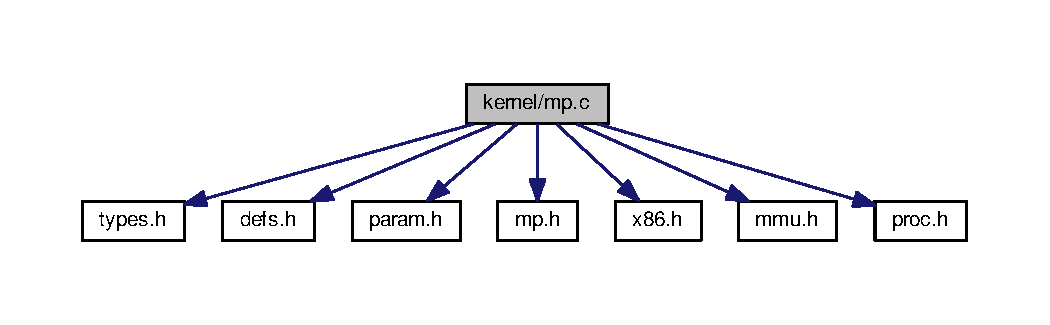
\includegraphics[width=350pt]{mp_8c__incl}
\end{center}
\end{figure}
\subsection*{Functions}
\begin{DoxyCompactItemize}
\item 
int \hyperlink{mp_8c_a0685a063c0d98b393f61e6c2cb5cdcba}{mpbcpu} (void)
\item 
void \hyperlink{mp_8c_a2fd0b66a17c5347541448ef906b7b2a2}{mpinit} (void)
\end{DoxyCompactItemize}
\subsection*{Variables}
\begin{DoxyCompactItemize}
\item 
struct \hyperlink{structcpu}{cpu} \hyperlink{mp_8c_a6d2633e73724907b582dfe6938ed7bb9}{cpus} \mbox{[}\hyperlink{param_8h_a2c4561c4c17cde39101c4e7a40d4492a}{N\-C\-P\-U}\mbox{]}
\item 
int \hyperlink{mp_8c_a46b52bd30030451d1b65291b77ba05d5}{ismp}
\item 
int \hyperlink{mp_8c_a6201a0661c3d5b88df5f63529298eb48}{ncpu}
\item 
\hyperlink{types_8h_a65f85814a8290f9797005d3b28e7e5fc}{uchar} \hyperlink{mp_8c_a619ae379337e3cb2397ee0b6b4fd8d6b}{ioapicid}
\end{DoxyCompactItemize}


\subsection{Function Documentation}
\hypertarget{mp_8c_a0685a063c0d98b393f61e6c2cb5cdcba}{\index{mp.\-c@{mp.\-c}!mpbcpu@{mpbcpu}}
\index{mpbcpu@{mpbcpu}!mp.c@{mp.\-c}}
\subsubsection[{mpbcpu}]{\setlength{\rightskip}{0pt plus 5cm}int mpbcpu (
\begin{DoxyParamCaption}
\item[{void}]{}
\end{DoxyParamCaption}
)}}\label{mp_8c_a0685a063c0d98b393f61e6c2cb5cdcba}


Definition at line 20 of file mp.\-c.

\hypertarget{mp_8c_a2fd0b66a17c5347541448ef906b7b2a2}{\index{mp.\-c@{mp.\-c}!mpinit@{mpinit}}
\index{mpinit@{mpinit}!mp.c@{mp.\-c}}
\subsubsection[{mpinit}]{\setlength{\rightskip}{0pt plus 5cm}void mpinit (
\begin{DoxyParamCaption}
\item[{void}]{}
\end{DoxyParamCaption}
)}}\label{mp_8c_a2fd0b66a17c5347541448ef906b7b2a2}


Definition at line 98 of file mp.\-c.



\subsection{Variable Documentation}
\hypertarget{mp_8c_a6d2633e73724907b582dfe6938ed7bb9}{\index{mp.\-c@{mp.\-c}!cpus@{cpus}}
\index{cpus@{cpus}!mp.c@{mp.\-c}}
\subsubsection[{cpus}]{\setlength{\rightskip}{0pt plus 5cm}struct {\bf cpu} cpus\mbox{[}{\bf N\-C\-P\-U}\mbox{]}}}\label{mp_8c_a6d2633e73724907b582dfe6938ed7bb9}


Definition at line 13 of file mp.\-c.

\hypertarget{mp_8c_a619ae379337e3cb2397ee0b6b4fd8d6b}{\index{mp.\-c@{mp.\-c}!ioapicid@{ioapicid}}
\index{ioapicid@{ioapicid}!mp.c@{mp.\-c}}
\subsubsection[{ioapicid}]{\setlength{\rightskip}{0pt plus 5cm}{\bf uchar} ioapicid}}\label{mp_8c_a619ae379337e3cb2397ee0b6b4fd8d6b}


Definition at line 17 of file mp.\-c.

\hypertarget{mp_8c_a46b52bd30030451d1b65291b77ba05d5}{\index{mp.\-c@{mp.\-c}!ismp@{ismp}}
\index{ismp@{ismp}!mp.c@{mp.\-c}}
\subsubsection[{ismp}]{\setlength{\rightskip}{0pt plus 5cm}int ismp}}\label{mp_8c_a46b52bd30030451d1b65291b77ba05d5}


Definition at line 15 of file mp.\-c.

\hypertarget{mp_8c_a6201a0661c3d5b88df5f63529298eb48}{\index{mp.\-c@{mp.\-c}!ncpu@{ncpu}}
\index{ncpu@{ncpu}!mp.c@{mp.\-c}}
\subsubsection[{ncpu}]{\setlength{\rightskip}{0pt plus 5cm}int ncpu}}\label{mp_8c_a6201a0661c3d5b88df5f63529298eb48}


Definition at line 16 of file mp.\-c.


\hypertarget{mp_8d}{\section{kernel/mp.d File Reference}
\label{mp_8d}\index{kernel/mp.\-d@{kernel/mp.\-d}}
}

\hypertarget{mp_8h}{\section{kernel/mp.h File Reference}
\label{mp_8h}\index{kernel/mp.\-h@{kernel/mp.\-h}}
}
This graph shows which files directly or indirectly include this file\-:
\nopagebreak
\begin{figure}[H]
\begin{center}
\leavevmode
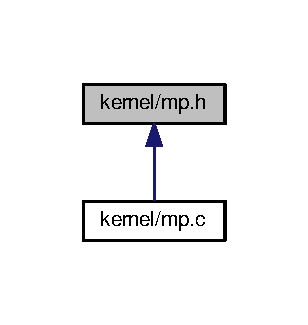
\includegraphics[width=148pt]{mp_8h__dep__incl}
\end{center}
\end{figure}
\subsection*{Data Structures}
\begin{DoxyCompactItemize}
\item 
struct \hyperlink{structmp}{mp}
\item 
struct \hyperlink{structmpconf}{mpconf}
\item 
struct \hyperlink{structmpproc}{mpproc}
\item 
struct \hyperlink{structmpioapic}{mpioapic}
\end{DoxyCompactItemize}
\subsection*{Macros}
\begin{DoxyCompactItemize}
\item 
\#define \hyperlink{mp_8h_ac167849b287b4ba22d110a1253bdd56d}{M\-P\-B\-O\-O\-T}~0x02
\item 
\#define \hyperlink{mp_8h_a0dd89a9c5a25d2d9f9a7fe57beb69597}{M\-P\-P\-R\-O\-C}~0x00
\item 
\#define \hyperlink{mp_8h_a10d8190eb1ea465310862131da282a09}{M\-P\-B\-U\-S}~0x01
\item 
\#define \hyperlink{mp_8h_a6d6b1d8666df6dc57974e608dda01edc}{M\-P\-I\-O\-A\-P\-I\-C}~0x02
\item 
\#define \hyperlink{mp_8h_a613c0cd2bca1e5a30eb1ffc7857d4d61}{M\-P\-I\-O\-I\-N\-T\-R}~0x03
\item 
\#define \hyperlink{mp_8h_a993af198877b836f019baaa9f12c7c30}{M\-P\-L\-I\-N\-T\-R}~0x04
\end{DoxyCompactItemize}


\subsection{Macro Definition Documentation}
\hypertarget{mp_8h_ac167849b287b4ba22d110a1253bdd56d}{\index{mp.\-h@{mp.\-h}!M\-P\-B\-O\-O\-T@{M\-P\-B\-O\-O\-T}}
\index{M\-P\-B\-O\-O\-T@{M\-P\-B\-O\-O\-T}!mp.h@{mp.\-h}}
\subsubsection[{M\-P\-B\-O\-O\-T}]{\setlength{\rightskip}{0pt plus 5cm}\#define M\-P\-B\-O\-O\-T~0x02}}\label{mp_8h_ac167849b287b4ba22d110a1253bdd56d}


Definition at line 36 of file mp.\-h.

\hypertarget{mp_8h_a10d8190eb1ea465310862131da282a09}{\index{mp.\-h@{mp.\-h}!M\-P\-B\-U\-S@{M\-P\-B\-U\-S}}
\index{M\-P\-B\-U\-S@{M\-P\-B\-U\-S}!mp.h@{mp.\-h}}
\subsubsection[{M\-P\-B\-U\-S}]{\setlength{\rightskip}{0pt plus 5cm}\#define M\-P\-B\-U\-S~0x01}}\label{mp_8h_a10d8190eb1ea465310862131da282a09}


Definition at line 52 of file mp.\-h.

\hypertarget{mp_8h_a6d6b1d8666df6dc57974e608dda01edc}{\index{mp.\-h@{mp.\-h}!M\-P\-I\-O\-A\-P\-I\-C@{M\-P\-I\-O\-A\-P\-I\-C}}
\index{M\-P\-I\-O\-A\-P\-I\-C@{M\-P\-I\-O\-A\-P\-I\-C}!mp.h@{mp.\-h}}
\subsubsection[{M\-P\-I\-O\-A\-P\-I\-C}]{\setlength{\rightskip}{0pt plus 5cm}\#define M\-P\-I\-O\-A\-P\-I\-C~0x02}}\label{mp_8h_a6d6b1d8666df6dc57974e608dda01edc}


Definition at line 53 of file mp.\-h.

\hypertarget{mp_8h_a613c0cd2bca1e5a30eb1ffc7857d4d61}{\index{mp.\-h@{mp.\-h}!M\-P\-I\-O\-I\-N\-T\-R@{M\-P\-I\-O\-I\-N\-T\-R}}
\index{M\-P\-I\-O\-I\-N\-T\-R@{M\-P\-I\-O\-I\-N\-T\-R}!mp.h@{mp.\-h}}
\subsubsection[{M\-P\-I\-O\-I\-N\-T\-R}]{\setlength{\rightskip}{0pt plus 5cm}\#define M\-P\-I\-O\-I\-N\-T\-R~0x03}}\label{mp_8h_a613c0cd2bca1e5a30eb1ffc7857d4d61}


Definition at line 54 of file mp.\-h.

\hypertarget{mp_8h_a993af198877b836f019baaa9f12c7c30}{\index{mp.\-h@{mp.\-h}!M\-P\-L\-I\-N\-T\-R@{M\-P\-L\-I\-N\-T\-R}}
\index{M\-P\-L\-I\-N\-T\-R@{M\-P\-L\-I\-N\-T\-R}!mp.h@{mp.\-h}}
\subsubsection[{M\-P\-L\-I\-N\-T\-R}]{\setlength{\rightskip}{0pt plus 5cm}\#define M\-P\-L\-I\-N\-T\-R~0x04}}\label{mp_8h_a993af198877b836f019baaa9f12c7c30}


Definition at line 55 of file mp.\-h.

\hypertarget{mp_8h_a0dd89a9c5a25d2d9f9a7fe57beb69597}{\index{mp.\-h@{mp.\-h}!M\-P\-P\-R\-O\-C@{M\-P\-P\-R\-O\-C}}
\index{M\-P\-P\-R\-O\-C@{M\-P\-P\-R\-O\-C}!mp.h@{mp.\-h}}
\subsubsection[{M\-P\-P\-R\-O\-C}]{\setlength{\rightskip}{0pt plus 5cm}\#define M\-P\-P\-R\-O\-C~0x00}}\label{mp_8h_a0dd89a9c5a25d2d9f9a7fe57beb69597}


Definition at line 51 of file mp.\-h.


\hypertarget{multiboot_8d}{\section{kernel/multiboot.d File Reference}
\label{multiboot_8d}\index{kernel/multiboot.\-d@{kernel/multiboot.\-d}}
}

\hypertarget{picirq_8c}{\section{kernel/picirq.c File Reference}
\label{picirq_8c}\index{kernel/picirq.\-c@{kernel/picirq.\-c}}
}
{\ttfamily \#include \char`\"{}types.\-h\char`\"{}}\\*
{\ttfamily \#include \char`\"{}x86.\-h\char`\"{}}\\*
{\ttfamily \#include \char`\"{}traps.\-h\char`\"{}}\\*
Include dependency graph for picirq.\-c\-:
\nopagebreak
\begin{figure}[H]
\begin{center}
\leavevmode
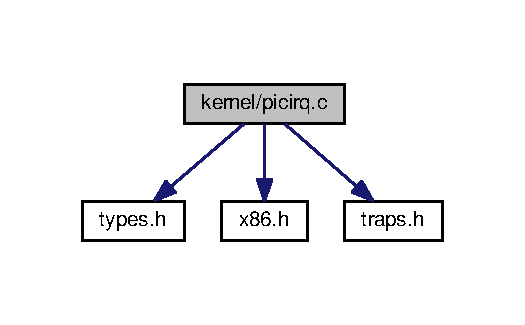
\includegraphics[width=252pt]{picirq_8c__incl}
\end{center}
\end{figure}
\subsection*{Macros}
\begin{DoxyCompactItemize}
\item 
\#define \hyperlink{picirq_8c_ad24a6214d0f5bb9bf67a8ac744907aa0}{I\-O\-\_\-\-P\-I\-C1}~0x20
\item 
\#define \hyperlink{picirq_8c_ab858a4b80bd8950398355e678c578d7d}{I\-O\-\_\-\-P\-I\-C2}~0x\-A0
\item 
\#define \hyperlink{picirq_8c_a6bd5318c8fa68a8ab5deb13d7ae4a6a7}{I\-R\-Q\-\_\-\-S\-L\-A\-V\-E}~2
\end{DoxyCompactItemize}
\subsection*{Functions}
\begin{DoxyCompactItemize}
\item 
void \hyperlink{picirq_8c_a8b8ecfe7680bc233db7c8695f2c16086}{picenable} (int irq)
\item 
void \hyperlink{picirq_8c_a8f19f54755d7fdec01e537228b10fbf6}{picinit} (void)
\end{DoxyCompactItemize}


\subsection{Macro Definition Documentation}
\hypertarget{picirq_8c_ad24a6214d0f5bb9bf67a8ac744907aa0}{\index{picirq.\-c@{picirq.\-c}!I\-O\-\_\-\-P\-I\-C1@{I\-O\-\_\-\-P\-I\-C1}}
\index{I\-O\-\_\-\-P\-I\-C1@{I\-O\-\_\-\-P\-I\-C1}!picirq.c@{picirq.\-c}}
\subsubsection[{I\-O\-\_\-\-P\-I\-C1}]{\setlength{\rightskip}{0pt plus 5cm}\#define I\-O\-\_\-\-P\-I\-C1~0x20}}\label{picirq_8c_ad24a6214d0f5bb9bf67a8ac744907aa0}


Definition at line 8 of file picirq.\-c.

\hypertarget{picirq_8c_ab858a4b80bd8950398355e678c578d7d}{\index{picirq.\-c@{picirq.\-c}!I\-O\-\_\-\-P\-I\-C2@{I\-O\-\_\-\-P\-I\-C2}}
\index{I\-O\-\_\-\-P\-I\-C2@{I\-O\-\_\-\-P\-I\-C2}!picirq.c@{picirq.\-c}}
\subsubsection[{I\-O\-\_\-\-P\-I\-C2}]{\setlength{\rightskip}{0pt plus 5cm}\#define I\-O\-\_\-\-P\-I\-C2~0x\-A0}}\label{picirq_8c_ab858a4b80bd8950398355e678c578d7d}


Definition at line 9 of file picirq.\-c.

\hypertarget{picirq_8c_a6bd5318c8fa68a8ab5deb13d7ae4a6a7}{\index{picirq.\-c@{picirq.\-c}!I\-R\-Q\-\_\-\-S\-L\-A\-V\-E@{I\-R\-Q\-\_\-\-S\-L\-A\-V\-E}}
\index{I\-R\-Q\-\_\-\-S\-L\-A\-V\-E@{I\-R\-Q\-\_\-\-S\-L\-A\-V\-E}!picirq.c@{picirq.\-c}}
\subsubsection[{I\-R\-Q\-\_\-\-S\-L\-A\-V\-E}]{\setlength{\rightskip}{0pt plus 5cm}\#define I\-R\-Q\-\_\-\-S\-L\-A\-V\-E~2}}\label{picirq_8c_a6bd5318c8fa68a8ab5deb13d7ae4a6a7}


Definition at line 11 of file picirq.\-c.



\subsection{Function Documentation}
\hypertarget{picirq_8c_a8b8ecfe7680bc233db7c8695f2c16086}{\index{picirq.\-c@{picirq.\-c}!picenable@{picenable}}
\index{picenable@{picenable}!picirq.c@{picirq.\-c}}
\subsubsection[{picenable}]{\setlength{\rightskip}{0pt plus 5cm}void picenable (
\begin{DoxyParamCaption}
\item[{int}]{irq}
\end{DoxyParamCaption}
)}}\label{picirq_8c_a8b8ecfe7680bc233db7c8695f2c16086}


Definition at line 26 of file picirq.\-c.

\hypertarget{picirq_8c_a8f19f54755d7fdec01e537228b10fbf6}{\index{picirq.\-c@{picirq.\-c}!picinit@{picinit}}
\index{picinit@{picinit}!picirq.c@{picirq.\-c}}
\subsubsection[{picinit}]{\setlength{\rightskip}{0pt plus 5cm}void picinit (
\begin{DoxyParamCaption}
\item[{void}]{}
\end{DoxyParamCaption}
)}}\label{picirq_8c_a8f19f54755d7fdec01e537228b10fbf6}


Definition at line 33 of file picirq.\-c.


\hypertarget{picirq_8d}{\section{kernel/picirq.d File Reference}
\label{picirq_8d}\index{kernel/picirq.\-d@{kernel/picirq.\-d}}
}

\hypertarget{pipe_8c}{\section{kernel/pipe.c File Reference}
\label{pipe_8c}\index{kernel/pipe.\-c@{kernel/pipe.\-c}}
}
{\ttfamily \#include \char`\"{}types.\-h\char`\"{}}\\*
{\ttfamily \#include \char`\"{}defs.\-h\char`\"{}}\\*
{\ttfamily \#include \char`\"{}param.\-h\char`\"{}}\\*
{\ttfamily \#include \char`\"{}mmu.\-h\char`\"{}}\\*
{\ttfamily \#include \char`\"{}proc.\-h\char`\"{}}\\*
{\ttfamily \#include \char`\"{}fs.\-h\char`\"{}}\\*
{\ttfamily \#include \char`\"{}file.\-h\char`\"{}}\\*
{\ttfamily \#include \char`\"{}spinlock.\-h\char`\"{}}\\*
Include dependency graph for pipe.\-c\-:
\nopagebreak
\begin{figure}[H]
\begin{center}
\leavevmode
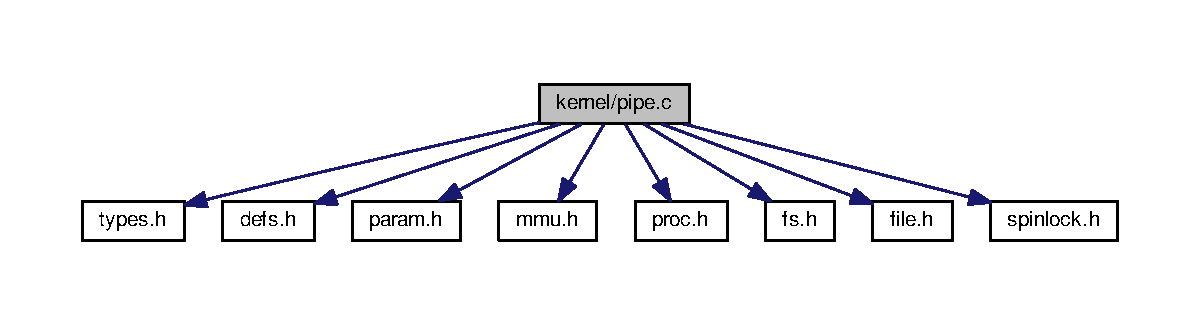
\includegraphics[width=350pt]{pipe_8c__incl}
\end{center}
\end{figure}
\subsection*{Data Structures}
\begin{DoxyCompactItemize}
\item 
struct \hyperlink{structpipe}{pipe}
\end{DoxyCompactItemize}
\subsection*{Macros}
\begin{DoxyCompactItemize}
\item 
\#define \hyperlink{pipe_8c_ad3dc9214a710d7a6c516cbaa2a12a1de}{P\-I\-P\-E\-S\-I\-Z\-E}~512
\end{DoxyCompactItemize}
\subsection*{Functions}
\begin{DoxyCompactItemize}
\item 
int \hyperlink{pipe_8c_a9d6f0c526148e6002b6776619c7563e6}{pipealloc} (struct \hyperlink{structfile}{file} $\ast$$\ast$f0, struct \hyperlink{structfile}{file} $\ast$$\ast$f1)
\item 
void \hyperlink{pipe_8c_a48642f54734698f6f881ee07723292cb}{pipeclose} (struct \hyperlink{structpipe}{pipe} $\ast$p, int writable)
\item 
int \hyperlink{pipe_8c_acfca0fab7d2c0c0dcc56359c8febe14a}{pipewrite} (struct \hyperlink{structpipe}{pipe} $\ast$p, char $\ast$addr, int n)
\item 
int \hyperlink{pipe_8c_ad4cce6144039b615d139f8660c60293a}{piperead} (struct \hyperlink{structpipe}{pipe} $\ast$p, char $\ast$addr, int n)
\end{DoxyCompactItemize}


\subsection{Macro Definition Documentation}
\hypertarget{pipe_8c_ad3dc9214a710d7a6c516cbaa2a12a1de}{\index{pipe.\-c@{pipe.\-c}!P\-I\-P\-E\-S\-I\-Z\-E@{P\-I\-P\-E\-S\-I\-Z\-E}}
\index{P\-I\-P\-E\-S\-I\-Z\-E@{P\-I\-P\-E\-S\-I\-Z\-E}!pipe.c@{pipe.\-c}}
\subsubsection[{P\-I\-P\-E\-S\-I\-Z\-E}]{\setlength{\rightskip}{0pt plus 5cm}\#define P\-I\-P\-E\-S\-I\-Z\-E~512}}\label{pipe_8c_ad3dc9214a710d7a6c516cbaa2a12a1de}


Definition at line 10 of file pipe.\-c.



\subsection{Function Documentation}
\hypertarget{pipe_8c_a9d6f0c526148e6002b6776619c7563e6}{\index{pipe.\-c@{pipe.\-c}!pipealloc@{pipealloc}}
\index{pipealloc@{pipealloc}!pipe.c@{pipe.\-c}}
\subsubsection[{pipealloc}]{\setlength{\rightskip}{0pt plus 5cm}int pipealloc (
\begin{DoxyParamCaption}
\item[{struct {\bf file} $\ast$$\ast$}]{f0, }
\item[{struct {\bf file} $\ast$$\ast$}]{f1}
\end{DoxyParamCaption}
)}}\label{pipe_8c_a9d6f0c526148e6002b6776619c7563e6}


Definition at line 22 of file pipe.\-c.

\hypertarget{pipe_8c_a48642f54734698f6f881ee07723292cb}{\index{pipe.\-c@{pipe.\-c}!pipeclose@{pipeclose}}
\index{pipeclose@{pipeclose}!pipe.c@{pipe.\-c}}
\subsubsection[{pipeclose}]{\setlength{\rightskip}{0pt plus 5cm}void pipeclose (
\begin{DoxyParamCaption}
\item[{struct {\bf pipe} $\ast$}]{p, }
\item[{int}]{writable}
\end{DoxyParamCaption}
)}}\label{pipe_8c_a48642f54734698f6f881ee07723292cb}


Definition at line 58 of file pipe.\-c.

\hypertarget{pipe_8c_ad4cce6144039b615d139f8660c60293a}{\index{pipe.\-c@{pipe.\-c}!piperead@{piperead}}
\index{piperead@{piperead}!pipe.c@{pipe.\-c}}
\subsubsection[{piperead}]{\setlength{\rightskip}{0pt plus 5cm}int piperead (
\begin{DoxyParamCaption}
\item[{struct {\bf pipe} $\ast$}]{p, }
\item[{char $\ast$}]{addr, }
\item[{int}]{n}
\end{DoxyParamCaption}
)}}\label{pipe_8c_ad4cce6144039b615d139f8660c60293a}


Definition at line 98 of file pipe.\-c.

\hypertarget{pipe_8c_acfca0fab7d2c0c0dcc56359c8febe14a}{\index{pipe.\-c@{pipe.\-c}!pipewrite@{pipewrite}}
\index{pipewrite@{pipewrite}!pipe.c@{pipe.\-c}}
\subsubsection[{pipewrite}]{\setlength{\rightskip}{0pt plus 5cm}int pipewrite (
\begin{DoxyParamCaption}
\item[{struct {\bf pipe} $\ast$}]{p, }
\item[{char $\ast$}]{addr, }
\item[{int}]{n}
\end{DoxyParamCaption}
)}}\label{pipe_8c_acfca0fab7d2c0c0dcc56359c8febe14a}


Definition at line 76 of file pipe.\-c.


\hypertarget{pipe_8d}{\section{kernel/pipe.d File Reference}
\label{pipe_8d}\index{kernel/pipe.\-d@{kernel/pipe.\-d}}
}

\hypertarget{proc_8c}{\section{kernel/proc.c File Reference}
\label{proc_8c}\index{kernel/proc.\-c@{kernel/proc.\-c}}
}
{\ttfamily \#include \char`\"{}types.\-h\char`\"{}}\\*
{\ttfamily \#include \char`\"{}defs.\-h\char`\"{}}\\*
{\ttfamily \#include \char`\"{}param.\-h\char`\"{}}\\*
{\ttfamily \#include \char`\"{}mmu.\-h\char`\"{}}\\*
{\ttfamily \#include \char`\"{}x86.\-h\char`\"{}}\\*
{\ttfamily \#include \char`\"{}proc.\-h\char`\"{}}\\*
{\ttfamily \#include \char`\"{}spinlock.\-h\char`\"{}}\\*
Include dependency graph for proc.\-c\-:
\nopagebreak
\begin{figure}[H]
\begin{center}
\leavevmode
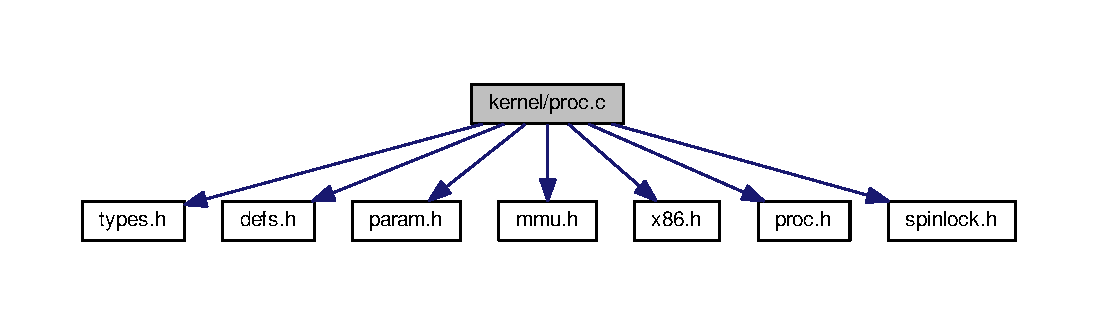
\includegraphics[width=350pt]{proc_8c__incl}
\end{center}
\end{figure}
\subsection*{Functions}
\begin{DoxyCompactItemize}
\item 
void \hyperlink{proc_8c_a11c5d62d28e8121e75235d361158156e}{forkret} (void)
\item 
void \hyperlink{proc_8c_a6c085102b25a17b9a1a78db5a8be16f9}{trapret} (void)
\item 
void \hyperlink{proc_8c_a9d293f913985937ee7a266fe5ddbfc77}{pinit} (void)
\item 
void \hyperlink{proc_8c_a81c8a6a0cae413bc81aa223f7f7b7205}{userinit} (void)
\item 
int \hyperlink{proc_8c_a9c16214741f4fcd088e5eea468709328}{growproc} (int n)
\item 
int \hyperlink{proc_8c_acd2e1ded4bb6fce4500438bf928330f4}{fork} (void)
\item 
void \hyperlink{proc_8c_aaf98ef7cdde3a0dfb2e49919de3298b1}{exit} (void)
\item 
int \hyperlink{proc_8c_af6f31822f7e737b4e414bdac1ccb59a4}{wait} (void)
\item 
void \hyperlink{proc_8c_a9fa00b0be5d3c4781048861e2506eb63}{scheduler} (void)
\item 
void \hyperlink{proc_8c_ad788da91743c333b5bed7c4a0dd12365}{sched} (void)
\item 
void \hyperlink{proc_8c_a7cb51f5c2b5cad3766f19eb69c92793b}{yield} (void)
\item 
void \hyperlink{proc_8c_ae70cc0370342e46f6db3bec367232457}{sleep} (void $\ast$chan, struct \hyperlink{structspinlock}{spinlock} $\ast$lk)
\item 
void \hyperlink{proc_8c_a4a34d9f03e436cfa09b88f735f6ee952}{wakeup} (void $\ast$chan)
\item 
int \hyperlink{proc_8c_a650cf0caaaa8b75f653c1c92818d03a4}{kill} (int pid)
\item 
void \hyperlink{proc_8c_a7f185044294ebb57521c73f723990164}{procdump} (void)
\end{DoxyCompactItemize}
\subsection*{Variables}
\begin{DoxyCompactItemize}
\item 
\begin{tabbing}
xx\=xx\=xx\=xx\=xx\=xx\=xx\=xx\=xx\=\kill
struct \{\\
\>struct \hyperlink{structspinlock}{spinlock} \hyperlink{proc_8c_ab28e82cd5dda7d960095706a3ea20572}{lock}\\
\>struct \hyperlink{structproc}{proc} \hyperlink{proc_8c_a5780b0050ca664736fd1cc9696624ce5}{proc} \mbox{[}\hyperlink{param_8h_a810c5b751df5bb30588613ed91095129}{NPROC}\mbox{]}\\
\} \hyperlink{proc_8c_af119fb7b095a8f6bff7e3d805371826f}{ptable}\\

\end{tabbing}\item 
int \hyperlink{proc_8c_aec016216766697de7529c7b9cb5beda9}{nextpid} = 1
\end{DoxyCompactItemize}


\subsection{Function Documentation}
\hypertarget{proc_8c_aaf98ef7cdde3a0dfb2e49919de3298b1}{\index{proc.\-c@{proc.\-c}!exit@{exit}}
\index{exit@{exit}!proc.c@{proc.\-c}}
\subsubsection[{exit}]{\setlength{\rightskip}{0pt plus 5cm}void exit (
\begin{DoxyParamCaption}
\item[{void}]{}
\end{DoxyParamCaption}
)}}\label{proc_8c_aaf98ef7cdde3a0dfb2e49919de3298b1}


Definition at line 166 of file proc.\-c.

\hypertarget{proc_8c_acd2e1ded4bb6fce4500438bf928330f4}{\index{proc.\-c@{proc.\-c}!fork@{fork}}
\index{fork@{fork}!proc.c@{proc.\-c}}
\subsubsection[{fork}]{\setlength{\rightskip}{0pt plus 5cm}int fork (
\begin{DoxyParamCaption}
\item[{void}]{}
\end{DoxyParamCaption}
)}}\label{proc_8c_acd2e1ded4bb6fce4500438bf928330f4}


Definition at line 128 of file proc.\-c.

\hypertarget{proc_8c_a11c5d62d28e8121e75235d361158156e}{\index{proc.\-c@{proc.\-c}!forkret@{forkret}}
\index{forkret@{forkret}!proc.c@{proc.\-c}}
\subsubsection[{forkret}]{\setlength{\rightskip}{0pt plus 5cm}void forkret (
\begin{DoxyParamCaption}
\item[{void}]{}
\end{DoxyParamCaption}
)}}\label{proc_8c_a11c5d62d28e8121e75235d361158156e}


Definition at line 321 of file proc.\-c.

\hypertarget{proc_8c_a9c16214741f4fcd088e5eea468709328}{\index{proc.\-c@{proc.\-c}!growproc@{growproc}}
\index{growproc@{growproc}!proc.c@{proc.\-c}}
\subsubsection[{growproc}]{\setlength{\rightskip}{0pt plus 5cm}int growproc (
\begin{DoxyParamCaption}
\item[{int}]{n}
\end{DoxyParamCaption}
)}}\label{proc_8c_a9c16214741f4fcd088e5eea468709328}


Definition at line 107 of file proc.\-c.

\hypertarget{proc_8c_a650cf0caaaa8b75f653c1c92818d03a4}{\index{proc.\-c@{proc.\-c}!kill@{kill}}
\index{kill@{kill}!proc.c@{proc.\-c}}
\subsubsection[{kill}]{\setlength{\rightskip}{0pt plus 5cm}int kill (
\begin{DoxyParamCaption}
\item[{int}]{pid}
\end{DoxyParamCaption}
)}}\label{proc_8c_a650cf0caaaa8b75f653c1c92818d03a4}


Definition at line 391 of file proc.\-c.

\hypertarget{proc_8c_a9d293f913985937ee7a266fe5ddbfc77}{\index{proc.\-c@{proc.\-c}!pinit@{pinit}}
\index{pinit@{pinit}!proc.c@{proc.\-c}}
\subsubsection[{pinit}]{\setlength{\rightskip}{0pt plus 5cm}void pinit (
\begin{DoxyParamCaption}
\item[{void}]{}
\end{DoxyParamCaption}
)}}\label{proc_8c_a9d293f913985937ee7a266fe5ddbfc77}


Definition at line 23 of file proc.\-c.

\hypertarget{proc_8c_a7f185044294ebb57521c73f723990164}{\index{proc.\-c@{proc.\-c}!procdump@{procdump}}
\index{procdump@{procdump}!proc.c@{proc.\-c}}
\subsubsection[{procdump}]{\setlength{\rightskip}{0pt plus 5cm}void procdump (
\begin{DoxyParamCaption}
\item[{void}]{}
\end{DoxyParamCaption}
)}}\label{proc_8c_a7f185044294ebb57521c73f723990164}


Definition at line 414 of file proc.\-c.

\hypertarget{proc_8c_ad788da91743c333b5bed7c4a0dd12365}{\index{proc.\-c@{proc.\-c}!sched@{sched}}
\index{sched@{sched}!proc.c@{proc.\-c}}
\subsubsection[{sched}]{\setlength{\rightskip}{0pt plus 5cm}void sched (
\begin{DoxyParamCaption}
\item[{void}]{}
\end{DoxyParamCaption}
)}}\label{proc_8c_ad788da91743c333b5bed7c4a0dd12365}


Definition at line 291 of file proc.\-c.

\hypertarget{proc_8c_a9fa00b0be5d3c4781048861e2506eb63}{\index{proc.\-c@{proc.\-c}!scheduler@{scheduler}}
\index{scheduler@{scheduler}!proc.c@{proc.\-c}}
\subsubsection[{scheduler}]{\setlength{\rightskip}{0pt plus 5cm}void scheduler (
\begin{DoxyParamCaption}
\item[{void}]{}
\end{DoxyParamCaption}
)}}\label{proc_8c_a9fa00b0be5d3c4781048861e2506eb63}


Definition at line 256 of file proc.\-c.

\hypertarget{proc_8c_ae70cc0370342e46f6db3bec367232457}{\index{proc.\-c@{proc.\-c}!sleep@{sleep}}
\index{sleep@{sleep}!proc.c@{proc.\-c}}
\subsubsection[{sleep}]{\setlength{\rightskip}{0pt plus 5cm}void sleep (
\begin{DoxyParamCaption}
\item[{void $\ast$}]{chan, }
\item[{struct {\bf spinlock} $\ast$}]{lk}
\end{DoxyParamCaption}
)}}\label{proc_8c_ae70cc0370342e46f6db3bec367232457}


Definition at line 332 of file proc.\-c.

\hypertarget{proc_8c_a6c085102b25a17b9a1a78db5a8be16f9}{\index{proc.\-c@{proc.\-c}!trapret@{trapret}}
\index{trapret@{trapret}!proc.c@{proc.\-c}}
\subsubsection[{trapret}]{\setlength{\rightskip}{0pt plus 5cm}void trapret (
\begin{DoxyParamCaption}
\item[{void}]{}
\end{DoxyParamCaption}
)}}\label{proc_8c_a6c085102b25a17b9a1a78db5a8be16f9}
\hypertarget{proc_8c_a81c8a6a0cae413bc81aa223f7f7b7205}{\index{proc.\-c@{proc.\-c}!userinit@{userinit}}
\index{userinit@{userinit}!proc.c@{proc.\-c}}
\subsubsection[{userinit}]{\setlength{\rightskip}{0pt plus 5cm}void userinit (
\begin{DoxyParamCaption}
\item[{void}]{}
\end{DoxyParamCaption}
)}}\label{proc_8c_a81c8a6a0cae413bc81aa223f7f7b7205}


Definition at line 76 of file proc.\-c.

\hypertarget{proc_8c_af6f31822f7e737b4e414bdac1ccb59a4}{\index{proc.\-c@{proc.\-c}!wait@{wait}}
\index{wait@{wait}!proc.c@{proc.\-c}}
\subsubsection[{wait}]{\setlength{\rightskip}{0pt plus 5cm}int wait (
\begin{DoxyParamCaption}
\item[{void}]{}
\end{DoxyParamCaption}
)}}\label{proc_8c_af6f31822f7e737b4e414bdac1ccb59a4}


Definition at line 208 of file proc.\-c.

\hypertarget{proc_8c_a4a34d9f03e436cfa09b88f735f6ee952}{\index{proc.\-c@{proc.\-c}!wakeup@{wakeup}}
\index{wakeup@{wakeup}!proc.c@{proc.\-c}}
\subsubsection[{wakeup}]{\setlength{\rightskip}{0pt plus 5cm}void wakeup (
\begin{DoxyParamCaption}
\item[{void $\ast$}]{chan}
\end{DoxyParamCaption}
)}}\label{proc_8c_a4a34d9f03e436cfa09b88f735f6ee952}


Definition at line 380 of file proc.\-c.

\hypertarget{proc_8c_a7cb51f5c2b5cad3766f19eb69c92793b}{\index{proc.\-c@{proc.\-c}!yield@{yield}}
\index{yield@{yield}!proc.c@{proc.\-c}}
\subsubsection[{yield}]{\setlength{\rightskip}{0pt plus 5cm}void yield (
\begin{DoxyParamCaption}
\item[{void}]{}
\end{DoxyParamCaption}
)}}\label{proc_8c_a7cb51f5c2b5cad3766f19eb69c92793b}


Definition at line 310 of file proc.\-c.



\subsection{Variable Documentation}
\hypertarget{proc_8c_ab28e82cd5dda7d960095706a3ea20572}{\index{proc.\-c@{proc.\-c}!lock@{lock}}
\index{lock@{lock}!proc.c@{proc.\-c}}
\subsubsection[{lock}]{\setlength{\rightskip}{0pt plus 5cm}struct {\bf spinlock} lock}}\label{proc_8c_ab28e82cd5dda7d960095706a3ea20572}


Definition at line 10 of file proc.\-c.

\hypertarget{proc_8c_aec016216766697de7529c7b9cb5beda9}{\index{proc.\-c@{proc.\-c}!nextpid@{nextpid}}
\index{nextpid@{nextpid}!proc.c@{proc.\-c}}
\subsubsection[{nextpid}]{\setlength{\rightskip}{0pt plus 5cm}int nextpid = 1}}\label{proc_8c_aec016216766697de7529c7b9cb5beda9}


Definition at line 16 of file proc.\-c.

\hypertarget{proc_8c_a5780b0050ca664736fd1cc9696624ce5}{\index{proc.\-c@{proc.\-c}!proc@{proc}}
\index{proc@{proc}!proc.c@{proc.\-c}}
\subsubsection[{proc}]{\setlength{\rightskip}{0pt plus 5cm}struct {\bf proc} {\bf proc}\mbox{[}{\bf N\-P\-R\-O\-C}\mbox{]}}}\label{proc_8c_a5780b0050ca664736fd1cc9696624ce5}


Definition at line 11 of file proc.\-c.

\hypertarget{proc_8c_af119fb7b095a8f6bff7e3d805371826f}{\index{proc.\-c@{proc.\-c}!ptable@{ptable}}
\index{ptable@{ptable}!proc.c@{proc.\-c}}
\subsubsection[{ptable}]{\setlength{\rightskip}{0pt plus 5cm}struct \{ ... \}   ptable}}\label{proc_8c_af119fb7b095a8f6bff7e3d805371826f}

\hypertarget{proc_8d}{\section{kernel/proc.d File Reference}
\label{proc_8d}\index{kernel/proc.\-d@{kernel/proc.\-d}}
}

\hypertarget{proc_8h}{\section{kernel/proc.h File Reference}
\label{proc_8h}\index{kernel/proc.\-h@{kernel/proc.\-h}}
}
This graph shows which files directly or indirectly include this file\-:
\nopagebreak
\begin{figure}[H]
\begin{center}
\leavevmode
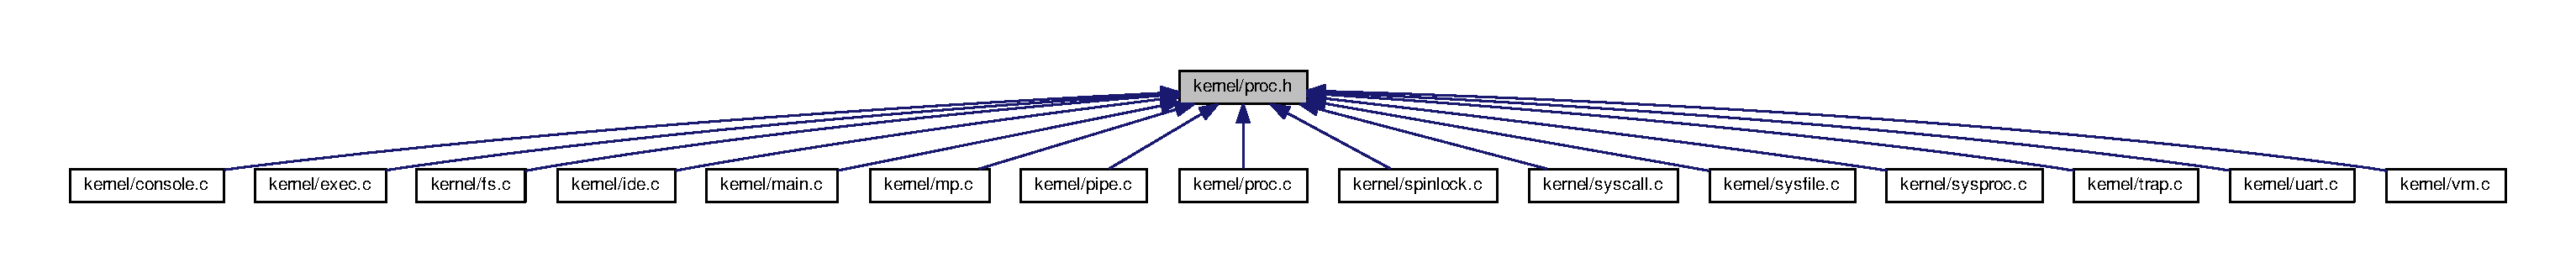
\includegraphics[width=350pt]{proc_8h__dep__incl}
\end{center}
\end{figure}
\subsection*{Data Structures}
\begin{DoxyCompactItemize}
\item 
struct \hyperlink{structcpu}{cpu}
\item 
struct \hyperlink{structcontext}{context}
\item 
struct \hyperlink{structproc}{proc}
\end{DoxyCompactItemize}
\subsection*{Macros}
\begin{DoxyCompactItemize}
\item 
\#define \hyperlink{proc_8h_a0d4e0c4c738af60d6092941469642429}{S\-E\-G\-\_\-\-K\-C\-O\-D\-E}~1
\item 
\#define \hyperlink{proc_8h_ad523d10217ef0ff5e75b7831f251d2b1}{S\-E\-G\-\_\-\-K\-D\-A\-T\-A}~2
\item 
\#define \hyperlink{proc_8h_a82120ac49072169c6f53657dc4b99e07}{S\-E\-G\-\_\-\-K\-C\-P\-U}~3
\item 
\#define \hyperlink{proc_8h_a85b694d969eb01e547197c21db219f4b}{S\-E\-G\-\_\-\-U\-C\-O\-D\-E}~4
\item 
\#define \hyperlink{proc_8h_aba0495696b4c656fda31704782648461}{S\-E\-G\-\_\-\-U\-D\-A\-T\-A}~5
\item 
\#define \hyperlink{proc_8h_a51332450caa8201ecc42fce428288e6f}{S\-E\-G\-\_\-\-T\-S\-S}~6
\item 
\#define \hyperlink{proc_8h_a2fca412c6ed6584438e96f43ccce030a}{N\-S\-E\-G\-S}~7
\end{DoxyCompactItemize}
\subsection*{Enumerations}
\begin{DoxyCompactItemize}
\item 
enum \hyperlink{proc_8h_aa1ced7d2b60040fded3fa873d0c03ba7}{procstate} \{ \\*
\hyperlink{proc_8h_aa1ced7d2b60040fded3fa873d0c03ba7aa09b651ef326a9d8efcee5cc5b720ab4}{U\-N\-U\-S\-E\-D}, 
\hyperlink{proc_8h_aa1ced7d2b60040fded3fa873d0c03ba7aaed0f3d976d25b54cb7c895ce591febb}{E\-M\-B\-R\-Y\-O}, 
\hyperlink{proc_8h_aa1ced7d2b60040fded3fa873d0c03ba7a488282601451a751e0f0e770b15d4235}{S\-L\-E\-E\-P\-I\-N\-G}, 
\hyperlink{proc_8h_aa1ced7d2b60040fded3fa873d0c03ba7a269b90433e40460a2c0044a0b3e15694}{R\-U\-N\-N\-A\-B\-L\-E}, 
\\*
\hyperlink{proc_8h_aa1ced7d2b60040fded3fa873d0c03ba7a1061be6c3fb88d32829cba6f6b2be304}{R\-U\-N\-N\-I\-N\-G}, 
\hyperlink{proc_8h_aa1ced7d2b60040fded3fa873d0c03ba7a5dfb36109b24f39d54d5c3f48f53def8}{Z\-O\-M\-B\-I\-E}
 \}
\end{DoxyCompactItemize}
\subsection*{Functions}
\begin{DoxyCompactItemize}
\item 
struct \hyperlink{structcpu}{cpu} $\ast$\hyperlink{structcpu}{cpu} \hyperlink{proc_8h_a878a634b88f305d27996e9c976dd76c3}{asm} (\char`\"{}\%gs\-:0\char`\"{})
\item 
struct \hyperlink{structproc}{proc} $\ast$\hyperlink{structproc}{proc} \hyperlink{proc_8h_a6424715dee020940c16737056af70edf}{asm} (\char`\"{}\%gs\-:4\char`\"{})
\end{DoxyCompactItemize}
\subsection*{Variables}
\begin{DoxyCompactItemize}
\item 
struct \hyperlink{structcpu}{cpu} \hyperlink{proc_8h_a6d2633e73724907b582dfe6938ed7bb9}{cpus} \mbox{[}\hyperlink{param_8h_a2c4561c4c17cde39101c4e7a40d4492a}{N\-C\-P\-U}\mbox{]}
\item 
int \hyperlink{proc_8h_a6201a0661c3d5b88df5f63529298eb48}{ncpu}
\end{DoxyCompactItemize}


\subsection{Macro Definition Documentation}
\hypertarget{proc_8h_a2fca412c6ed6584438e96f43ccce030a}{\index{proc.\-h@{proc.\-h}!N\-S\-E\-G\-S@{N\-S\-E\-G\-S}}
\index{N\-S\-E\-G\-S@{N\-S\-E\-G\-S}!proc.h@{proc.\-h}}
\subsubsection[{N\-S\-E\-G\-S}]{\setlength{\rightskip}{0pt plus 5cm}\#define N\-S\-E\-G\-S~7}}\label{proc_8h_a2fca412c6ed6584438e96f43ccce030a}


Definition at line 11 of file proc.\-h.

\hypertarget{proc_8h_a0d4e0c4c738af60d6092941469642429}{\index{proc.\-h@{proc.\-h}!S\-E\-G\-\_\-\-K\-C\-O\-D\-E@{S\-E\-G\-\_\-\-K\-C\-O\-D\-E}}
\index{S\-E\-G\-\_\-\-K\-C\-O\-D\-E@{S\-E\-G\-\_\-\-K\-C\-O\-D\-E}!proc.h@{proc.\-h}}
\subsubsection[{S\-E\-G\-\_\-\-K\-C\-O\-D\-E}]{\setlength{\rightskip}{0pt plus 5cm}\#define S\-E\-G\-\_\-\-K\-C\-O\-D\-E~1}}\label{proc_8h_a0d4e0c4c738af60d6092941469642429}


Definition at line 5 of file proc.\-h.

\hypertarget{proc_8h_a82120ac49072169c6f53657dc4b99e07}{\index{proc.\-h@{proc.\-h}!S\-E\-G\-\_\-\-K\-C\-P\-U@{S\-E\-G\-\_\-\-K\-C\-P\-U}}
\index{S\-E\-G\-\_\-\-K\-C\-P\-U@{S\-E\-G\-\_\-\-K\-C\-P\-U}!proc.h@{proc.\-h}}
\subsubsection[{S\-E\-G\-\_\-\-K\-C\-P\-U}]{\setlength{\rightskip}{0pt plus 5cm}\#define S\-E\-G\-\_\-\-K\-C\-P\-U~3}}\label{proc_8h_a82120ac49072169c6f53657dc4b99e07}


Definition at line 7 of file proc.\-h.

\hypertarget{proc_8h_ad523d10217ef0ff5e75b7831f251d2b1}{\index{proc.\-h@{proc.\-h}!S\-E\-G\-\_\-\-K\-D\-A\-T\-A@{S\-E\-G\-\_\-\-K\-D\-A\-T\-A}}
\index{S\-E\-G\-\_\-\-K\-D\-A\-T\-A@{S\-E\-G\-\_\-\-K\-D\-A\-T\-A}!proc.h@{proc.\-h}}
\subsubsection[{S\-E\-G\-\_\-\-K\-D\-A\-T\-A}]{\setlength{\rightskip}{0pt plus 5cm}\#define S\-E\-G\-\_\-\-K\-D\-A\-T\-A~2}}\label{proc_8h_ad523d10217ef0ff5e75b7831f251d2b1}


Definition at line 6 of file proc.\-h.

\hypertarget{proc_8h_a51332450caa8201ecc42fce428288e6f}{\index{proc.\-h@{proc.\-h}!S\-E\-G\-\_\-\-T\-S\-S@{S\-E\-G\-\_\-\-T\-S\-S}}
\index{S\-E\-G\-\_\-\-T\-S\-S@{S\-E\-G\-\_\-\-T\-S\-S}!proc.h@{proc.\-h}}
\subsubsection[{S\-E\-G\-\_\-\-T\-S\-S}]{\setlength{\rightskip}{0pt plus 5cm}\#define S\-E\-G\-\_\-\-T\-S\-S~6}}\label{proc_8h_a51332450caa8201ecc42fce428288e6f}


Definition at line 10 of file proc.\-h.

\hypertarget{proc_8h_a85b694d969eb01e547197c21db219f4b}{\index{proc.\-h@{proc.\-h}!S\-E\-G\-\_\-\-U\-C\-O\-D\-E@{S\-E\-G\-\_\-\-U\-C\-O\-D\-E}}
\index{S\-E\-G\-\_\-\-U\-C\-O\-D\-E@{S\-E\-G\-\_\-\-U\-C\-O\-D\-E}!proc.h@{proc.\-h}}
\subsubsection[{S\-E\-G\-\_\-\-U\-C\-O\-D\-E}]{\setlength{\rightskip}{0pt plus 5cm}\#define S\-E\-G\-\_\-\-U\-C\-O\-D\-E~4}}\label{proc_8h_a85b694d969eb01e547197c21db219f4b}


Definition at line 8 of file proc.\-h.

\hypertarget{proc_8h_aba0495696b4c656fda31704782648461}{\index{proc.\-h@{proc.\-h}!S\-E\-G\-\_\-\-U\-D\-A\-T\-A@{S\-E\-G\-\_\-\-U\-D\-A\-T\-A}}
\index{S\-E\-G\-\_\-\-U\-D\-A\-T\-A@{S\-E\-G\-\_\-\-U\-D\-A\-T\-A}!proc.h@{proc.\-h}}
\subsubsection[{S\-E\-G\-\_\-\-U\-D\-A\-T\-A}]{\setlength{\rightskip}{0pt plus 5cm}\#define S\-E\-G\-\_\-\-U\-D\-A\-T\-A~5}}\label{proc_8h_aba0495696b4c656fda31704782648461}


Definition at line 9 of file proc.\-h.



\subsection{Enumeration Type Documentation}
\hypertarget{proc_8h_aa1ced7d2b60040fded3fa873d0c03ba7}{\index{proc.\-h@{proc.\-h}!procstate@{procstate}}
\index{procstate@{procstate}!proc.h@{proc.\-h}}
\subsubsection[{procstate}]{\setlength{\rightskip}{0pt plus 5cm}enum {\bf procstate}}}\label{proc_8h_aa1ced7d2b60040fded3fa873d0c03ba7}
\begin{Desc}
\item[Enumerator]\par
\begin{description}
\index{U\-N\-U\-S\-E\-D@{U\-N\-U\-S\-E\-D}!proc.\-h@{proc.\-h}}\index{proc.\-h@{proc.\-h}!U\-N\-U\-S\-E\-D@{U\-N\-U\-S\-E\-D}}\item[{\em 
\hypertarget{proc_8h_aa1ced7d2b60040fded3fa873d0c03ba7aa09b651ef326a9d8efcee5cc5b720ab4}{U\-N\-U\-S\-E\-D}\label{proc_8h_aa1ced7d2b60040fded3fa873d0c03ba7aa09b651ef326a9d8efcee5cc5b720ab4}
}]\index{E\-M\-B\-R\-Y\-O@{E\-M\-B\-R\-Y\-O}!proc.\-h@{proc.\-h}}\index{proc.\-h@{proc.\-h}!E\-M\-B\-R\-Y\-O@{E\-M\-B\-R\-Y\-O}}\item[{\em 
\hypertarget{proc_8h_aa1ced7d2b60040fded3fa873d0c03ba7aaed0f3d976d25b54cb7c895ce591febb}{E\-M\-B\-R\-Y\-O}\label{proc_8h_aa1ced7d2b60040fded3fa873d0c03ba7aaed0f3d976d25b54cb7c895ce591febb}
}]\index{S\-L\-E\-E\-P\-I\-N\-G@{S\-L\-E\-E\-P\-I\-N\-G}!proc.\-h@{proc.\-h}}\index{proc.\-h@{proc.\-h}!S\-L\-E\-E\-P\-I\-N\-G@{S\-L\-E\-E\-P\-I\-N\-G}}\item[{\em 
\hypertarget{proc_8h_aa1ced7d2b60040fded3fa873d0c03ba7a488282601451a751e0f0e770b15d4235}{S\-L\-E\-E\-P\-I\-N\-G}\label{proc_8h_aa1ced7d2b60040fded3fa873d0c03ba7a488282601451a751e0f0e770b15d4235}
}]\index{R\-U\-N\-N\-A\-B\-L\-E@{R\-U\-N\-N\-A\-B\-L\-E}!proc.\-h@{proc.\-h}}\index{proc.\-h@{proc.\-h}!R\-U\-N\-N\-A\-B\-L\-E@{R\-U\-N\-N\-A\-B\-L\-E}}\item[{\em 
\hypertarget{proc_8h_aa1ced7d2b60040fded3fa873d0c03ba7a269b90433e40460a2c0044a0b3e15694}{R\-U\-N\-N\-A\-B\-L\-E}\label{proc_8h_aa1ced7d2b60040fded3fa873d0c03ba7a269b90433e40460a2c0044a0b3e15694}
}]\index{R\-U\-N\-N\-I\-N\-G@{R\-U\-N\-N\-I\-N\-G}!proc.\-h@{proc.\-h}}\index{proc.\-h@{proc.\-h}!R\-U\-N\-N\-I\-N\-G@{R\-U\-N\-N\-I\-N\-G}}\item[{\em 
\hypertarget{proc_8h_aa1ced7d2b60040fded3fa873d0c03ba7a1061be6c3fb88d32829cba6f6b2be304}{R\-U\-N\-N\-I\-N\-G}\label{proc_8h_aa1ced7d2b60040fded3fa873d0c03ba7a1061be6c3fb88d32829cba6f6b2be304}
}]\index{Z\-O\-M\-B\-I\-E@{Z\-O\-M\-B\-I\-E}!proc.\-h@{proc.\-h}}\index{proc.\-h@{proc.\-h}!Z\-O\-M\-B\-I\-E@{Z\-O\-M\-B\-I\-E}}\item[{\em 
\hypertarget{proc_8h_aa1ced7d2b60040fded3fa873d0c03ba7a5dfb36109b24f39d54d5c3f48f53def8}{Z\-O\-M\-B\-I\-E}\label{proc_8h_aa1ced7d2b60040fded3fa873d0c03ba7a5dfb36109b24f39d54d5c3f48f53def8}
}]\end{description}
\end{Desc}


Definition at line 60 of file proc.\-h.



\subsection{Function Documentation}
\hypertarget{proc_8h_a878a634b88f305d27996e9c976dd76c3}{\index{proc.\-h@{proc.\-h}!asm@{asm}}
\index{asm@{asm}!proc.h@{proc.\-h}}
\subsubsection[{asm}]{\setlength{\rightskip}{0pt plus 5cm}struct {\bf cpu}$\ast$ {\bf cpu} asm (
\begin{DoxyParamCaption}
\item[{\char`\"{}\%gs\-:0\char`\"{}}]{}
\end{DoxyParamCaption}
)}}\label{proc_8h_a878a634b88f305d27996e9c976dd76c3}
\hypertarget{proc_8h_a6424715dee020940c16737056af70edf}{\index{proc.\-h@{proc.\-h}!asm@{asm}}
\index{asm@{asm}!proc.h@{proc.\-h}}
\subsubsection[{asm}]{\setlength{\rightskip}{0pt plus 5cm}struct {\bf proc}$\ast$ {\bf proc} asm (
\begin{DoxyParamCaption}
\item[{\char`\"{}\%gs\-:4\char`\"{}}]{}
\end{DoxyParamCaption}
)}}\label{proc_8h_a6424715dee020940c16737056af70edf}


\subsection{Variable Documentation}
\hypertarget{proc_8h_a6d2633e73724907b582dfe6938ed7bb9}{\index{proc.\-h@{proc.\-h}!cpus@{cpus}}
\index{cpus@{cpus}!proc.h@{proc.\-h}}
\subsubsection[{cpus}]{\setlength{\rightskip}{0pt plus 5cm}struct {\bf cpu} cpus\mbox{[}{\bf N\-C\-P\-U}\mbox{]}}}\label{proc_8h_a6d2633e73724907b582dfe6938ed7bb9}


Definition at line 13 of file mp.\-c.

\hypertarget{proc_8h_a6201a0661c3d5b88df5f63529298eb48}{\index{proc.\-h@{proc.\-h}!ncpu@{ncpu}}
\index{ncpu@{ncpu}!proc.h@{proc.\-h}}
\subsubsection[{ncpu}]{\setlength{\rightskip}{0pt plus 5cm}int ncpu}}\label{proc_8h_a6201a0661c3d5b88df5f63529298eb48}


Definition at line 16 of file mp.\-c.


\hypertarget{spinlock_8c}{\section{kernel/spinlock.c File Reference}
\label{spinlock_8c}\index{kernel/spinlock.\-c@{kernel/spinlock.\-c}}
}
{\ttfamily \#include \char`\"{}types.\-h\char`\"{}}\\*
{\ttfamily \#include \char`\"{}defs.\-h\char`\"{}}\\*
{\ttfamily \#include \char`\"{}param.\-h\char`\"{}}\\*
{\ttfamily \#include \char`\"{}x86.\-h\char`\"{}}\\*
{\ttfamily \#include \char`\"{}mmu.\-h\char`\"{}}\\*
{\ttfamily \#include \char`\"{}proc.\-h\char`\"{}}\\*
{\ttfamily \#include \char`\"{}spinlock.\-h\char`\"{}}\\*
Include dependency graph for spinlock.\-c\-:
\nopagebreak
\begin{figure}[H]
\begin{center}
\leavevmode
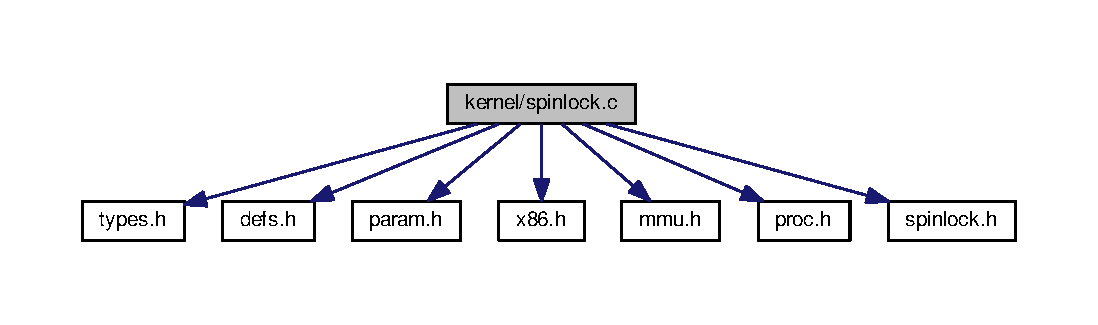
\includegraphics[width=350pt]{spinlock_8c__incl}
\end{center}
\end{figure}
\subsection*{Functions}
\begin{DoxyCompactItemize}
\item 
void \hyperlink{spinlock_8c_abda07b4a007b2e888d9d783920460b89}{initlock} (struct \hyperlink{structspinlock}{spinlock} $\ast$lk, char $\ast$\hyperlink{usertests_8c_aee754febd402311e2a552cb0d6ab6629}{name})
\item 
void \hyperlink{spinlock_8c_aed377f16a085b00de3a4b32392adbdfb}{acquire} (struct \hyperlink{structspinlock}{spinlock} $\ast$lk)
\item 
void \hyperlink{spinlock_8c_a1cee376aa9a00e754bf5481cd5f3d97b}{release} (struct \hyperlink{structspinlock}{spinlock} $\ast$lk)
\item 
void \hyperlink{spinlock_8c_a6ac35304ea80f01086b47edcc2328010}{getcallerpcs} (void $\ast$v, \hyperlink{types_8h_a91ad9478d81a7aaf2593e8d9c3d06a14}{uint} pcs\mbox{[}$\,$\mbox{]})
\item 
int \hyperlink{spinlock_8c_aea48df3e5cfb903179ad3dc78ab502d9}{holding} (struct \hyperlink{structspinlock}{spinlock} $\ast$\hyperlink{proc_8c_ab28e82cd5dda7d960095706a3ea20572}{lock})
\item 
void \hyperlink{spinlock_8c_a206b749d1b7768dadce61cbcde7e0f1c}{pushcli} (void)
\item 
void \hyperlink{spinlock_8c_ae3424f669269fef400ce29c3aeb43fdb}{popcli} (void)
\end{DoxyCompactItemize}


\subsection{Function Documentation}
\hypertarget{spinlock_8c_aed377f16a085b00de3a4b32392adbdfb}{\index{spinlock.\-c@{spinlock.\-c}!acquire@{acquire}}
\index{acquire@{acquire}!spinlock.c@{spinlock.\-c}}
\subsubsection[{acquire}]{\setlength{\rightskip}{0pt plus 5cm}void acquire (
\begin{DoxyParamCaption}
\item[{struct {\bf spinlock} $\ast$}]{lk}
\end{DoxyParamCaption}
)}}\label{spinlock_8c_aed377f16a085b00de3a4b32392adbdfb}


Definition at line 24 of file spinlock.\-c.

\hypertarget{spinlock_8c_a6ac35304ea80f01086b47edcc2328010}{\index{spinlock.\-c@{spinlock.\-c}!getcallerpcs@{getcallerpcs}}
\index{getcallerpcs@{getcallerpcs}!spinlock.c@{spinlock.\-c}}
\subsubsection[{getcallerpcs}]{\setlength{\rightskip}{0pt plus 5cm}void getcallerpcs (
\begin{DoxyParamCaption}
\item[{void $\ast$}]{v, }
\item[{{\bf uint}}]{pcs\mbox{[}$\,$\mbox{]}}
\end{DoxyParamCaption}
)}}\label{spinlock_8c_a6ac35304ea80f01086b47edcc2328010}


Definition at line 67 of file spinlock.\-c.

\hypertarget{spinlock_8c_aea48df3e5cfb903179ad3dc78ab502d9}{\index{spinlock.\-c@{spinlock.\-c}!holding@{holding}}
\index{holding@{holding}!spinlock.c@{spinlock.\-c}}
\subsubsection[{holding}]{\setlength{\rightskip}{0pt plus 5cm}int holding (
\begin{DoxyParamCaption}
\item[{struct {\bf spinlock} $\ast$}]{lock}
\end{DoxyParamCaption}
)}}\label{spinlock_8c_aea48df3e5cfb903179ad3dc78ab502d9}


Definition at line 85 of file spinlock.\-c.

\hypertarget{spinlock_8c_abda07b4a007b2e888d9d783920460b89}{\index{spinlock.\-c@{spinlock.\-c}!initlock@{initlock}}
\index{initlock@{initlock}!spinlock.c@{spinlock.\-c}}
\subsubsection[{initlock}]{\setlength{\rightskip}{0pt plus 5cm}void initlock (
\begin{DoxyParamCaption}
\item[{struct {\bf spinlock} $\ast$}]{lk, }
\item[{char $\ast$}]{name}
\end{DoxyParamCaption}
)}}\label{spinlock_8c_abda07b4a007b2e888d9d783920460b89}


Definition at line 12 of file spinlock.\-c.

\hypertarget{spinlock_8c_ae3424f669269fef400ce29c3aeb43fdb}{\index{spinlock.\-c@{spinlock.\-c}!popcli@{popcli}}
\index{popcli@{popcli}!spinlock.c@{spinlock.\-c}}
\subsubsection[{popcli}]{\setlength{\rightskip}{0pt plus 5cm}void popcli (
\begin{DoxyParamCaption}
\item[{void}]{}
\end{DoxyParamCaption}
)}}\label{spinlock_8c_ae3424f669269fef400ce29c3aeb43fdb}


Definition at line 107 of file spinlock.\-c.

\hypertarget{spinlock_8c_a206b749d1b7768dadce61cbcde7e0f1c}{\index{spinlock.\-c@{spinlock.\-c}!pushcli@{pushcli}}
\index{pushcli@{pushcli}!spinlock.c@{spinlock.\-c}}
\subsubsection[{pushcli}]{\setlength{\rightskip}{0pt plus 5cm}void pushcli (
\begin{DoxyParamCaption}
\item[{void}]{}
\end{DoxyParamCaption}
)}}\label{spinlock_8c_a206b749d1b7768dadce61cbcde7e0f1c}


Definition at line 96 of file spinlock.\-c.

\hypertarget{spinlock_8c_a1cee376aa9a00e754bf5481cd5f3d97b}{\index{spinlock.\-c@{spinlock.\-c}!release@{release}}
\index{release@{release}!spinlock.c@{spinlock.\-c}}
\subsubsection[{release}]{\setlength{\rightskip}{0pt plus 5cm}void release (
\begin{DoxyParamCaption}
\item[{struct {\bf spinlock} $\ast$}]{lk}
\end{DoxyParamCaption}
)}}\label{spinlock_8c_a1cee376aa9a00e754bf5481cd5f3d97b}


Definition at line 43 of file spinlock.\-c.


\hypertarget{spinlock_8d}{\section{kernel/spinlock.d File Reference}
\label{spinlock_8d}\index{kernel/spinlock.\-d@{kernel/spinlock.\-d}}
}

\hypertarget{spinlock_8h}{\section{kernel/spinlock.h File Reference}
\label{spinlock_8h}\index{kernel/spinlock.\-h@{kernel/spinlock.\-h}}
}
This graph shows which files directly or indirectly include this file\-:
\nopagebreak
\begin{figure}[H]
\begin{center}
\leavevmode
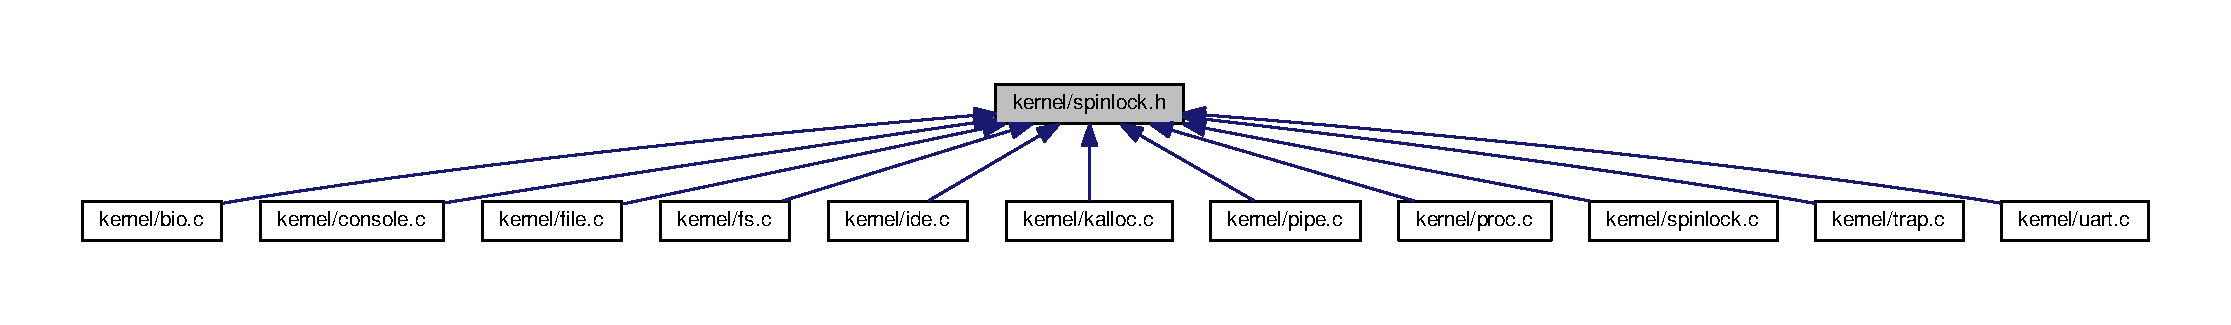
\includegraphics[width=350pt]{spinlock_8h__dep__incl}
\end{center}
\end{figure}
\subsection*{Data Structures}
\begin{DoxyCompactItemize}
\item 
struct \hyperlink{structspinlock}{spinlock}
\end{DoxyCompactItemize}

\hypertarget{string_8c}{\section{kernel/string.c File Reference}
\label{string_8c}\index{kernel/string.\-c@{kernel/string.\-c}}
}
{\ttfamily \#include \char`\"{}types.\-h\char`\"{}}\\*
{\ttfamily \#include \char`\"{}x86.\-h\char`\"{}}\\*
Include dependency graph for string.\-c\-:
\nopagebreak
\begin{figure}[H]
\begin{center}
\leavevmode
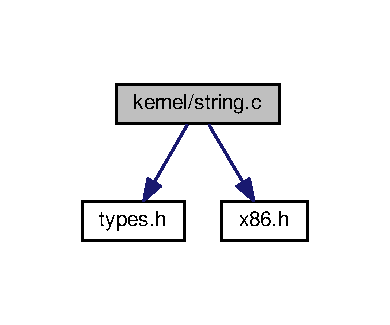
\includegraphics[width=187pt]{string_8c__incl}
\end{center}
\end{figure}
\subsection*{Functions}
\begin{DoxyCompactItemize}
\item 
void $\ast$ \hyperlink{string_8c_acbd02c899d9723092ddf5f8a4df32b33}{memset} (void $\ast$dst, int c, \hyperlink{types_8h_a91ad9478d81a7aaf2593e8d9c3d06a14}{uint} n)
\item 
int \hyperlink{string_8c_aa70027bbf4ef8a7388150c5b374f9b16}{memcmp} (const void $\ast$v1, const void $\ast$v2, \hyperlink{types_8h_a91ad9478d81a7aaf2593e8d9c3d06a14}{uint} n)
\item 
void $\ast$ \hyperlink{string_8c_a01f8724ac478257f6703f2a52c738323}{memmove} (void $\ast$dst, const void $\ast$src, \hyperlink{types_8h_a91ad9478d81a7aaf2593e8d9c3d06a14}{uint} n)
\item 
void $\ast$ \hyperlink{string_8c_ae3d71b1daca36f00293a5e21c342feb0}{memcpy} (void $\ast$dst, const void $\ast$src, \hyperlink{types_8h_a91ad9478d81a7aaf2593e8d9c3d06a14}{uint} n)
\item 
int \hyperlink{string_8c_a81b6f58fa9c826f064fb6844dda4c475}{strncmp} (const char $\ast$p, const char $\ast$q, \hyperlink{types_8h_a91ad9478d81a7aaf2593e8d9c3d06a14}{uint} n)
\item 
char $\ast$ \hyperlink{string_8c_a4ab1c467e4230b2b3bf6fc13ede30a57}{strncpy} (char $\ast$s, const char $\ast$t, int n)
\item 
char $\ast$ \hyperlink{string_8c_ad0571c1087565c892b1097c3ed677d61}{safestrcpy} (char $\ast$s, const char $\ast$t, int n)
\item 
int \hyperlink{string_8c_a2dee044e4e667b5b789b493abd21cfa4}{strlen} (const char $\ast$s)
\end{DoxyCompactItemize}


\subsection{Function Documentation}
\hypertarget{string_8c_aa70027bbf4ef8a7388150c5b374f9b16}{\index{string.\-c@{string.\-c}!memcmp@{memcmp}}
\index{memcmp@{memcmp}!string.c@{string.\-c}}
\subsubsection[{memcmp}]{\setlength{\rightskip}{0pt plus 5cm}int memcmp (
\begin{DoxyParamCaption}
\item[{const void $\ast$}]{v1, }
\item[{const void $\ast$}]{v2, }
\item[{{\bf uint}}]{n}
\end{DoxyParamCaption}
)}}\label{string_8c_aa70027bbf4ef8a7388150c5b374f9b16}


Definition at line 12 of file string.\-c.

\hypertarget{string_8c_ae3d71b1daca36f00293a5e21c342feb0}{\index{string.\-c@{string.\-c}!memcpy@{memcpy}}
\index{memcpy@{memcpy}!string.c@{string.\-c}}
\subsubsection[{memcpy}]{\setlength{\rightskip}{0pt plus 5cm}void$\ast$ memcpy (
\begin{DoxyParamCaption}
\item[{void $\ast$}]{dst, }
\item[{const void $\ast$}]{src, }
\item[{{\bf uint}}]{n}
\end{DoxyParamCaption}
)}}\label{string_8c_ae3d71b1daca36f00293a5e21c342feb0}


Definition at line 49 of file string.\-c.

\hypertarget{string_8c_a01f8724ac478257f6703f2a52c738323}{\index{string.\-c@{string.\-c}!memmove@{memmove}}
\index{memmove@{memmove}!string.c@{string.\-c}}
\subsubsection[{memmove}]{\setlength{\rightskip}{0pt plus 5cm}void$\ast$ memmove (
\begin{DoxyParamCaption}
\item[{void $\ast$}]{dst, }
\item[{const void $\ast$}]{src, }
\item[{{\bf uint}}]{n}
\end{DoxyParamCaption}
)}}\label{string_8c_a01f8724ac478257f6703f2a52c738323}


Definition at line 28 of file string.\-c.

\hypertarget{string_8c_acbd02c899d9723092ddf5f8a4df32b33}{\index{string.\-c@{string.\-c}!memset@{memset}}
\index{memset@{memset}!string.c@{string.\-c}}
\subsubsection[{memset}]{\setlength{\rightskip}{0pt plus 5cm}void$\ast$ memset (
\begin{DoxyParamCaption}
\item[{void $\ast$}]{dst, }
\item[{int}]{c, }
\item[{{\bf uint}}]{n}
\end{DoxyParamCaption}
)}}\label{string_8c_acbd02c899d9723092ddf5f8a4df32b33}


Definition at line 5 of file string.\-c.

\hypertarget{string_8c_ad0571c1087565c892b1097c3ed677d61}{\index{string.\-c@{string.\-c}!safestrcpy@{safestrcpy}}
\index{safestrcpy@{safestrcpy}!string.c@{string.\-c}}
\subsubsection[{safestrcpy}]{\setlength{\rightskip}{0pt plus 5cm}char$\ast$ safestrcpy (
\begin{DoxyParamCaption}
\item[{char $\ast$}]{s, }
\item[{const char $\ast$}]{t, }
\item[{int}]{n}
\end{DoxyParamCaption}
)}}\label{string_8c_ad0571c1087565c892b1097c3ed677d61}


Definition at line 79 of file string.\-c.

\hypertarget{string_8c_a2dee044e4e667b5b789b493abd21cfa4}{\index{string.\-c@{string.\-c}!strlen@{strlen}}
\index{strlen@{strlen}!string.c@{string.\-c}}
\subsubsection[{strlen}]{\setlength{\rightskip}{0pt plus 5cm}int strlen (
\begin{DoxyParamCaption}
\item[{const char $\ast$}]{s}
\end{DoxyParamCaption}
)}}\label{string_8c_a2dee044e4e667b5b789b493abd21cfa4}


Definition at line 93 of file string.\-c.

\hypertarget{string_8c_a81b6f58fa9c826f064fb6844dda4c475}{\index{string.\-c@{string.\-c}!strncmp@{strncmp}}
\index{strncmp@{strncmp}!string.c@{string.\-c}}
\subsubsection[{strncmp}]{\setlength{\rightskip}{0pt plus 5cm}int strncmp (
\begin{DoxyParamCaption}
\item[{const char $\ast$}]{p, }
\item[{const char $\ast$}]{q, }
\item[{{\bf uint}}]{n}
\end{DoxyParamCaption}
)}}\label{string_8c_a81b6f58fa9c826f064fb6844dda4c475}


Definition at line 55 of file string.\-c.

\hypertarget{string_8c_a4ab1c467e4230b2b3bf6fc13ede30a57}{\index{string.\-c@{string.\-c}!strncpy@{strncpy}}
\index{strncpy@{strncpy}!string.c@{string.\-c}}
\subsubsection[{strncpy}]{\setlength{\rightskip}{0pt plus 5cm}char$\ast$ strncpy (
\begin{DoxyParamCaption}
\item[{char $\ast$}]{s, }
\item[{const char $\ast$}]{t, }
\item[{int}]{n}
\end{DoxyParamCaption}
)}}\label{string_8c_a4ab1c467e4230b2b3bf6fc13ede30a57}


Definition at line 65 of file string.\-c.


\hypertarget{string_8d}{\section{kernel/string.d File Reference}
\label{string_8d}\index{kernel/string.\-d@{kernel/string.\-d}}
}

\hypertarget{swtch_8d}{\section{kernel/swtch.d File Reference}
\label{swtch_8d}\index{kernel/swtch.\-d@{kernel/swtch.\-d}}
}

\hypertarget{syscall_8c}{\section{kernel/syscall.c File Reference}
\label{syscall_8c}\index{kernel/syscall.\-c@{kernel/syscall.\-c}}
}
{\ttfamily \#include \char`\"{}types.\-h\char`\"{}}\\*
{\ttfamily \#include \char`\"{}defs.\-h\char`\"{}}\\*
{\ttfamily \#include \char`\"{}param.\-h\char`\"{}}\\*
{\ttfamily \#include \char`\"{}mmu.\-h\char`\"{}}\\*
{\ttfamily \#include \char`\"{}proc.\-h\char`\"{}}\\*
{\ttfamily \#include \char`\"{}x86.\-h\char`\"{}}\\*
{\ttfamily \#include \char`\"{}syscall.\-h\char`\"{}}\\*
{\ttfamily \#include \char`\"{}sysfunc.\-h\char`\"{}}\\*
Include dependency graph for syscall.\-c\-:
\nopagebreak
\begin{figure}[H]
\begin{center}
\leavevmode
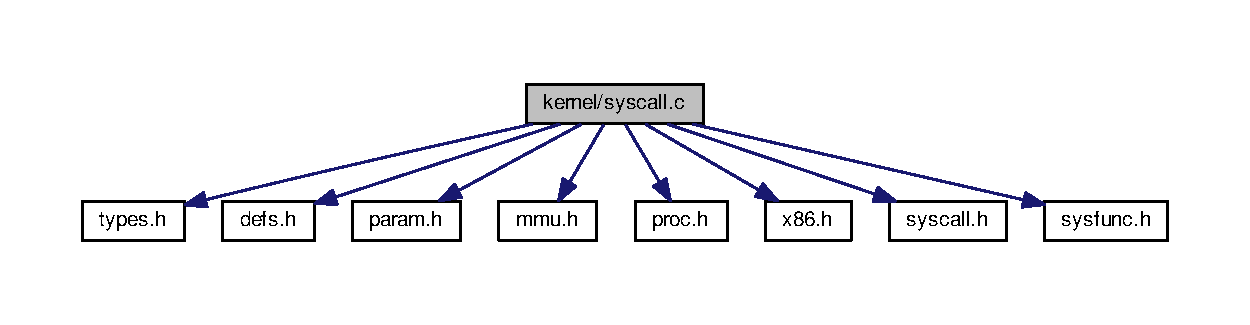
\includegraphics[width=350pt]{syscall_8c__incl}
\end{center}
\end{figure}
\subsection*{Functions}
\begin{DoxyCompactItemize}
\item 
int \hyperlink{syscall_8c_a68e387cd28d033ae0ae49e18ae587b95}{fetchint} (struct \hyperlink{structproc}{proc} $\ast$p, \hyperlink{types_8h_a91ad9478d81a7aaf2593e8d9c3d06a14}{uint} addr, int $\ast$ip)
\item 
int \hyperlink{syscall_8c_a02cf8a775688c8d936f5f6e19fe90f3a}{fetchstr} (struct \hyperlink{structproc}{proc} $\ast$p, \hyperlink{types_8h_a91ad9478d81a7aaf2593e8d9c3d06a14}{uint} addr, char $\ast$$\ast$pp)
\item 
int \hyperlink{syscall_8c_ade56ef2176f85cd61e7b91b400e7d4d3}{argint} (int n, int $\ast$ip)
\item 
int \hyperlink{syscall_8c_a6ade9205d1f46b759cf93b60513a3421}{argptr} (int n, char $\ast$$\ast$pp, int \hyperlink{mkfs_8c_a439227feff9d7f55384e8780cfc2eb82}{size})
\item 
int \hyperlink{syscall_8c_a662eedd65f3e2165093842b80e3bc024}{argstr} (int n, char $\ast$$\ast$pp)
\item 
void \hyperlink{syscall_8c_acd6bcafe6626fe8e7d00cacdbc3cc4f1}{syscall} (void)
\end{DoxyCompactItemize}


\subsection{Function Documentation}
\hypertarget{syscall_8c_ade56ef2176f85cd61e7b91b400e7d4d3}{\index{syscall.\-c@{syscall.\-c}!argint@{argint}}
\index{argint@{argint}!syscall.c@{syscall.\-c}}
\subsubsection[{argint}]{\setlength{\rightskip}{0pt plus 5cm}int argint (
\begin{DoxyParamCaption}
\item[{int}]{n, }
\item[{int $\ast$}]{ip}
\end{DoxyParamCaption}
)}}\label{syscall_8c_ade56ef2176f85cd61e7b91b400e7d4d3}


Definition at line 46 of file syscall.\-c.

\hypertarget{syscall_8c_a6ade9205d1f46b759cf93b60513a3421}{\index{syscall.\-c@{syscall.\-c}!argptr@{argptr}}
\index{argptr@{argptr}!syscall.c@{syscall.\-c}}
\subsubsection[{argptr}]{\setlength{\rightskip}{0pt plus 5cm}int argptr (
\begin{DoxyParamCaption}
\item[{int}]{n, }
\item[{char $\ast$$\ast$}]{pp, }
\item[{int}]{size}
\end{DoxyParamCaption}
)}}\label{syscall_8c_a6ade9205d1f46b759cf93b60513a3421}


Definition at line 55 of file syscall.\-c.

\hypertarget{syscall_8c_a662eedd65f3e2165093842b80e3bc024}{\index{syscall.\-c@{syscall.\-c}!argstr@{argstr}}
\index{argstr@{argstr}!syscall.c@{syscall.\-c}}
\subsubsection[{argstr}]{\setlength{\rightskip}{0pt plus 5cm}int argstr (
\begin{DoxyParamCaption}
\item[{int}]{n, }
\item[{char $\ast$$\ast$}]{pp}
\end{DoxyParamCaption}
)}}\label{syscall_8c_a662eedd65f3e2165093842b80e3bc024}


Definition at line 72 of file syscall.\-c.

\hypertarget{syscall_8c_a68e387cd28d033ae0ae49e18ae587b95}{\index{syscall.\-c@{syscall.\-c}!fetchint@{fetchint}}
\index{fetchint@{fetchint}!syscall.c@{syscall.\-c}}
\subsubsection[{fetchint}]{\setlength{\rightskip}{0pt plus 5cm}int fetchint (
\begin{DoxyParamCaption}
\item[{struct {\bf proc} $\ast$}]{p, }
\item[{{\bf uint}}]{addr, }
\item[{int $\ast$}]{ip}
\end{DoxyParamCaption}
)}}\label{syscall_8c_a68e387cd28d033ae0ae49e18ae587b95}


Definition at line 18 of file syscall.\-c.

\hypertarget{syscall_8c_a02cf8a775688c8d936f5f6e19fe90f3a}{\index{syscall.\-c@{syscall.\-c}!fetchstr@{fetchstr}}
\index{fetchstr@{fetchstr}!syscall.c@{syscall.\-c}}
\subsubsection[{fetchstr}]{\setlength{\rightskip}{0pt plus 5cm}int fetchstr (
\begin{DoxyParamCaption}
\item[{struct {\bf proc} $\ast$}]{p, }
\item[{{\bf uint}}]{addr, }
\item[{char $\ast$$\ast$}]{pp}
\end{DoxyParamCaption}
)}}\label{syscall_8c_a02cf8a775688c8d936f5f6e19fe90f3a}


Definition at line 30 of file syscall.\-c.

\hypertarget{syscall_8c_acd6bcafe6626fe8e7d00cacdbc3cc4f1}{\index{syscall.\-c@{syscall.\-c}!syscall@{syscall}}
\index{syscall@{syscall}!syscall.c@{syscall.\-c}}
\subsubsection[{syscall}]{\setlength{\rightskip}{0pt plus 5cm}void syscall (
\begin{DoxyParamCaption}
\item[{void}]{}
\end{DoxyParamCaption}
)}}\label{syscall_8c_acd6bcafe6626fe8e7d00cacdbc3cc4f1}


Definition at line 111 of file syscall.\-c.


\hypertarget{syscall_8d}{\section{kernel/syscall.d File Reference}
\label{syscall_8d}\index{kernel/syscall.\-d@{kernel/syscall.\-d}}
}

\hypertarget{sysfile_8c}{\section{kernel/sysfile.c File Reference}
\label{sysfile_8c}\index{kernel/sysfile.\-c@{kernel/sysfile.\-c}}
}
{\ttfamily \#include \char`\"{}types.\-h\char`\"{}}\\*
{\ttfamily \#include \char`\"{}defs.\-h\char`\"{}}\\*
{\ttfamily \#include \char`\"{}param.\-h\char`\"{}}\\*
{\ttfamily \#include \char`\"{}stat.\-h\char`\"{}}\\*
{\ttfamily \#include \char`\"{}mmu.\-h\char`\"{}}\\*
{\ttfamily \#include \char`\"{}proc.\-h\char`\"{}}\\*
{\ttfamily \#include \char`\"{}fs.\-h\char`\"{}}\\*
{\ttfamily \#include \char`\"{}file.\-h\char`\"{}}\\*
{\ttfamily \#include \char`\"{}fcntl.\-h\char`\"{}}\\*
{\ttfamily \#include \char`\"{}sysfunc.\-h\char`\"{}}\\*
Include dependency graph for sysfile.\-c\-:
\nopagebreak
\begin{figure}[H]
\begin{center}
\leavevmode
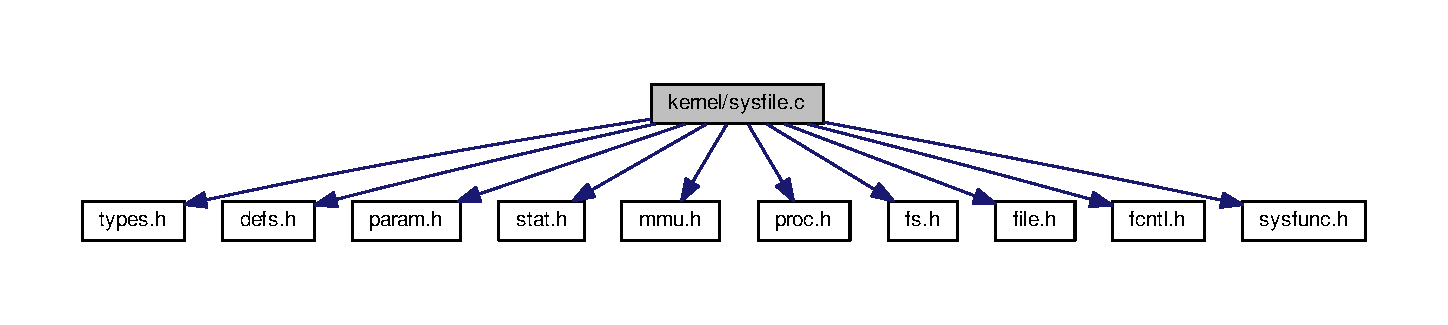
\includegraphics[width=350pt]{sysfile_8c__incl}
\end{center}
\end{figure}
\subsection*{Functions}
\begin{DoxyCompactItemize}
\item 
int \hyperlink{sysfile_8c_a8f8b9e2d98e8b444f23a39ae8992feff}{sys\-\_\-dup} (void)
\item 
int \hyperlink{sysfile_8c_a54bf714d9e898cbdcbc061b280bbfae0}{sys\-\_\-read} (void)
\item 
int \hyperlink{sysfile_8c_a687d939a9e4792af15db96f2c2f34378}{sys\-\_\-write} (void)
\item 
int \hyperlink{sysfile_8c_a32945488fd39bc405757177b37cd2250}{sys\-\_\-close} (void)
\item 
int \hyperlink{sysfile_8c_ac243c8f20f5fb2e3e257b5007af2c204}{sys\-\_\-fstat} (void)
\item 
int \hyperlink{sysfile_8c_a759600870314007ac558871239122fb7}{sys\-\_\-link} (void)
\item 
int \hyperlink{sysfile_8c_ae1e58ee11d41f643929520d8c1640da7}{sys\-\_\-unlink} (void)
\item 
int \hyperlink{sysfile_8c_a74e45efc661ca17c068bc283b3842e6d}{sys\-\_\-open} (void)
\item 
int \hyperlink{sysfile_8c_a057e5bce2de7a87ebfd2dc33967bca4a}{sys\-\_\-mkdir} (void)
\item 
int \hyperlink{sysfile_8c_a25697aa3d828b5878d38170d724adb27}{sys\-\_\-mknod} (void)
\item 
int \hyperlink{sysfile_8c_ad1c5f8693cb35b9605fee09eebdda640}{sys\-\_\-chdir} (void)
\item 
int \hyperlink{sysfile_8c_aeaa813ddeb6a5fac3c45714c7351c526}{sys\-\_\-exec} (void)
\item 
int \hyperlink{sysfile_8c_a9a70db941def46ec25939e6c2d30e399}{sys\-\_\-pipe} (void)
\end{DoxyCompactItemize}


\subsection{Function Documentation}
\hypertarget{sysfile_8c_ad1c5f8693cb35b9605fee09eebdda640}{\index{sysfile.\-c@{sysfile.\-c}!sys\-\_\-chdir@{sys\-\_\-chdir}}
\index{sys\-\_\-chdir@{sys\-\_\-chdir}!sysfile.c@{sysfile.\-c}}
\subsubsection[{sys\-\_\-chdir}]{\setlength{\rightskip}{0pt plus 5cm}int sys\-\_\-chdir (
\begin{DoxyParamCaption}
\item[{void}]{}
\end{DoxyParamCaption}
)}}\label{sysfile_8c_ad1c5f8693cb35b9605fee09eebdda640}


Definition at line 326 of file sysfile.\-c.

\hypertarget{sysfile_8c_a32945488fd39bc405757177b37cd2250}{\index{sysfile.\-c@{sysfile.\-c}!sys\-\_\-close@{sys\-\_\-close}}
\index{sys\-\_\-close@{sys\-\_\-close}!sysfile.c@{sysfile.\-c}}
\subsubsection[{sys\-\_\-close}]{\setlength{\rightskip}{0pt plus 5cm}int sys\-\_\-close (
\begin{DoxyParamCaption}
\item[{void}]{}
\end{DoxyParamCaption}
)}}\label{sysfile_8c_a32945488fd39bc405757177b37cd2250}


Definition at line 86 of file sysfile.\-c.

\hypertarget{sysfile_8c_a8f8b9e2d98e8b444f23a39ae8992feff}{\index{sysfile.\-c@{sysfile.\-c}!sys\-\_\-dup@{sys\-\_\-dup}}
\index{sys\-\_\-dup@{sys\-\_\-dup}!sysfile.c@{sysfile.\-c}}
\subsubsection[{sys\-\_\-dup}]{\setlength{\rightskip}{0pt plus 5cm}int sys\-\_\-dup (
\begin{DoxyParamCaption}
\item[{void}]{}
\end{DoxyParamCaption}
)}}\label{sysfile_8c_a8f8b9e2d98e8b444f23a39ae8992feff}


Definition at line 48 of file sysfile.\-c.

\hypertarget{sysfile_8c_aeaa813ddeb6a5fac3c45714c7351c526}{\index{sysfile.\-c@{sysfile.\-c}!sys\-\_\-exec@{sys\-\_\-exec}}
\index{sys\-\_\-exec@{sys\-\_\-exec}!sysfile.c@{sysfile.\-c}}
\subsubsection[{sys\-\_\-exec}]{\setlength{\rightskip}{0pt plus 5cm}int sys\-\_\-exec (
\begin{DoxyParamCaption}
\item[{void}]{}
\end{DoxyParamCaption}
)}}\label{sysfile_8c_aeaa813ddeb6a5fac3c45714c7351c526}


Definition at line 345 of file sysfile.\-c.

\hypertarget{sysfile_8c_ac243c8f20f5fb2e3e257b5007af2c204}{\index{sysfile.\-c@{sysfile.\-c}!sys\-\_\-fstat@{sys\-\_\-fstat}}
\index{sys\-\_\-fstat@{sys\-\_\-fstat}!sysfile.c@{sysfile.\-c}}
\subsubsection[{sys\-\_\-fstat}]{\setlength{\rightskip}{0pt plus 5cm}int sys\-\_\-fstat (
\begin{DoxyParamCaption}
\item[{void}]{}
\end{DoxyParamCaption}
)}}\label{sysfile_8c_ac243c8f20f5fb2e3e257b5007af2c204}


Definition at line 99 of file sysfile.\-c.

\hypertarget{sysfile_8c_a759600870314007ac558871239122fb7}{\index{sysfile.\-c@{sysfile.\-c}!sys\-\_\-link@{sys\-\_\-link}}
\index{sys\-\_\-link@{sys\-\_\-link}!sysfile.c@{sysfile.\-c}}
\subsubsection[{sys\-\_\-link}]{\setlength{\rightskip}{0pt plus 5cm}int sys\-\_\-link (
\begin{DoxyParamCaption}
\item[{void}]{}
\end{DoxyParamCaption}
)}}\label{sysfile_8c_a759600870314007ac558871239122fb7}


Definition at line 111 of file sysfile.\-c.

\hypertarget{sysfile_8c_a057e5bce2de7a87ebfd2dc33967bca4a}{\index{sysfile.\-c@{sysfile.\-c}!sys\-\_\-mkdir@{sys\-\_\-mkdir}}
\index{sys\-\_\-mkdir@{sys\-\_\-mkdir}!sysfile.c@{sysfile.\-c}}
\subsubsection[{sys\-\_\-mkdir}]{\setlength{\rightskip}{0pt plus 5cm}int sys\-\_\-mkdir (
\begin{DoxyParamCaption}
\item[{void}]{}
\end{DoxyParamCaption}
)}}\label{sysfile_8c_a057e5bce2de7a87ebfd2dc33967bca4a}


Definition at line 297 of file sysfile.\-c.

\hypertarget{sysfile_8c_a25697aa3d828b5878d38170d724adb27}{\index{sysfile.\-c@{sysfile.\-c}!sys\-\_\-mknod@{sys\-\_\-mknod}}
\index{sys\-\_\-mknod@{sys\-\_\-mknod}!sysfile.c@{sysfile.\-c}}
\subsubsection[{sys\-\_\-mknod}]{\setlength{\rightskip}{0pt plus 5cm}int sys\-\_\-mknod (
\begin{DoxyParamCaption}
\item[{void}]{}
\end{DoxyParamCaption}
)}}\label{sysfile_8c_a25697aa3d828b5878d38170d724adb27}


Definition at line 309 of file sysfile.\-c.

\hypertarget{sysfile_8c_a74e45efc661ca17c068bc283b3842e6d}{\index{sysfile.\-c@{sysfile.\-c}!sys\-\_\-open@{sys\-\_\-open}}
\index{sys\-\_\-open@{sys\-\_\-open}!sysfile.c@{sysfile.\-c}}
\subsubsection[{sys\-\_\-open}]{\setlength{\rightskip}{0pt plus 5cm}int sys\-\_\-open (
\begin{DoxyParamCaption}
\item[{void}]{}
\end{DoxyParamCaption}
)}}\label{sysfile_8c_a74e45efc661ca17c068bc283b3842e6d}


Definition at line 258 of file sysfile.\-c.

\hypertarget{sysfile_8c_a9a70db941def46ec25939e6c2d30e399}{\index{sysfile.\-c@{sysfile.\-c}!sys\-\_\-pipe@{sys\-\_\-pipe}}
\index{sys\-\_\-pipe@{sys\-\_\-pipe}!sysfile.c@{sysfile.\-c}}
\subsubsection[{sys\-\_\-pipe}]{\setlength{\rightskip}{0pt plus 5cm}int sys\-\_\-pipe (
\begin{DoxyParamCaption}
\item[{void}]{}
\end{DoxyParamCaption}
)}}\label{sysfile_8c_a9a70db941def46ec25939e6c2d30e399}


Definition at line 371 of file sysfile.\-c.

\hypertarget{sysfile_8c_a54bf714d9e898cbdcbc061b280bbfae0}{\index{sysfile.\-c@{sysfile.\-c}!sys\-\_\-read@{sys\-\_\-read}}
\index{sys\-\_\-read@{sys\-\_\-read}!sysfile.c@{sysfile.\-c}}
\subsubsection[{sys\-\_\-read}]{\setlength{\rightskip}{0pt plus 5cm}int sys\-\_\-read (
\begin{DoxyParamCaption}
\item[{void}]{}
\end{DoxyParamCaption}
)}}\label{sysfile_8c_a54bf714d9e898cbdcbc061b280bbfae0}


Definition at line 62 of file sysfile.\-c.

\hypertarget{sysfile_8c_ae1e58ee11d41f643929520d8c1640da7}{\index{sysfile.\-c@{sysfile.\-c}!sys\-\_\-unlink@{sys\-\_\-unlink}}
\index{sys\-\_\-unlink@{sys\-\_\-unlink}!sysfile.c@{sysfile.\-c}}
\subsubsection[{sys\-\_\-unlink}]{\setlength{\rightskip}{0pt plus 5cm}int sys\-\_\-unlink (
\begin{DoxyParamCaption}
\item[{void}]{}
\end{DoxyParamCaption}
)}}\label{sysfile_8c_ae1e58ee11d41f643929520d8c1640da7}


Definition at line 165 of file sysfile.\-c.

\hypertarget{sysfile_8c_a687d939a9e4792af15db96f2c2f34378}{\index{sysfile.\-c@{sysfile.\-c}!sys\-\_\-write@{sys\-\_\-write}}
\index{sys\-\_\-write@{sys\-\_\-write}!sysfile.c@{sysfile.\-c}}
\subsubsection[{sys\-\_\-write}]{\setlength{\rightskip}{0pt plus 5cm}int sys\-\_\-write (
\begin{DoxyParamCaption}
\item[{void}]{}
\end{DoxyParamCaption}
)}}\label{sysfile_8c_a687d939a9e4792af15db96f2c2f34378}


Definition at line 74 of file sysfile.\-c.


\hypertarget{sysfile_8d}{\section{kernel/sysfile.d File Reference}
\label{sysfile_8d}\index{kernel/sysfile.\-d@{kernel/sysfile.\-d}}
}

\hypertarget{sysfunc_8h}{\section{kernel/sysfunc.h File Reference}
\label{sysfunc_8h}\index{kernel/sysfunc.\-h@{kernel/sysfunc.\-h}}
}
This graph shows which files directly or indirectly include this file\-:
\nopagebreak
\begin{figure}[H]
\begin{center}
\leavevmode
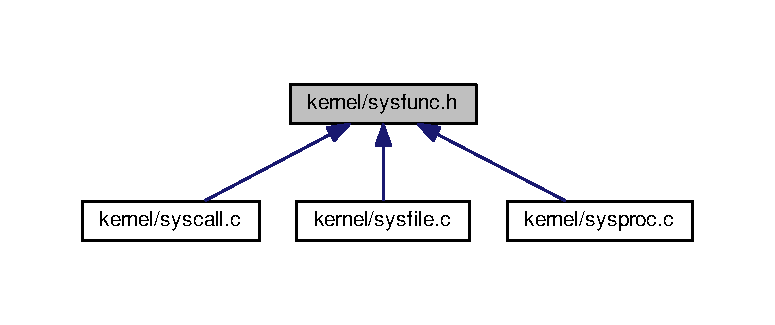
\includegraphics[width=350pt]{sysfunc_8h__dep__incl}
\end{center}
\end{figure}
\subsection*{Functions}
\begin{DoxyCompactItemize}
\item 
int \hyperlink{sysfunc_8h_ad1c5f8693cb35b9605fee09eebdda640}{sys\-\_\-chdir} (void)
\item 
int \hyperlink{sysfunc_8h_a32945488fd39bc405757177b37cd2250}{sys\-\_\-close} (void)
\item 
int \hyperlink{sysfunc_8h_a8f8b9e2d98e8b444f23a39ae8992feff}{sys\-\_\-dup} (void)
\item 
int \hyperlink{sysfunc_8h_aeaa813ddeb6a5fac3c45714c7351c526}{sys\-\_\-exec} (void)
\item 
int \hyperlink{sysfunc_8h_aee72faa31a0c32b410aba558ef1d59f2}{sys\-\_\-exit} (void)
\item 
int \hyperlink{sysfunc_8h_a3b05102e512b34446a54334f916ba5cd}{sys\-\_\-fork} (void)
\item 
int \hyperlink{sysfunc_8h_ac243c8f20f5fb2e3e257b5007af2c204}{sys\-\_\-fstat} (void)
\item 
int \hyperlink{sysfunc_8h_ac81965412a0725574b8c72afda11243e}{sys\-\_\-getpid} (void)
\item 
int \hyperlink{sysfunc_8h_ad766b54842470b464a6497bb5c514e59}{sys\-\_\-kill} (void)
\item 
int \hyperlink{sysfunc_8h_a759600870314007ac558871239122fb7}{sys\-\_\-link} (void)
\item 
int \hyperlink{sysfunc_8h_a057e5bce2de7a87ebfd2dc33967bca4a}{sys\-\_\-mkdir} (void)
\item 
int \hyperlink{sysfunc_8h_a25697aa3d828b5878d38170d724adb27}{sys\-\_\-mknod} (void)
\item 
int \hyperlink{sysfunc_8h_a74e45efc661ca17c068bc283b3842e6d}{sys\-\_\-open} (void)
\item 
int \hyperlink{sysfunc_8h_a9a70db941def46ec25939e6c2d30e399}{sys\-\_\-pipe} (void)
\item 
int \hyperlink{sysfunc_8h_a54bf714d9e898cbdcbc061b280bbfae0}{sys\-\_\-read} (void)
\item 
int \hyperlink{sysfunc_8h_ab21d46be776cf6075a997af525a1a628}{sys\-\_\-sbrk} (void)
\item 
int \hyperlink{sysfunc_8h_a59778ec9bfa6b6f2100b43fbba000573}{sys\-\_\-sleep} (void)
\item 
int \hyperlink{sysfunc_8h_ae1e58ee11d41f643929520d8c1640da7}{sys\-\_\-unlink} (void)
\item 
int \hyperlink{sysfunc_8h_ad202e06addda05ba6fe60f05d3f61913}{sys\-\_\-wait} (void)
\item 
int \hyperlink{sysfunc_8h_a687d939a9e4792af15db96f2c2f34378}{sys\-\_\-write} (void)
\item 
int \hyperlink{sysfunc_8h_aaf8553903ba8f2776247679d4db0d121}{sys\-\_\-uptime} (void)
\end{DoxyCompactItemize}


\subsection{Function Documentation}
\hypertarget{sysfunc_8h_ad1c5f8693cb35b9605fee09eebdda640}{\index{sysfunc.\-h@{sysfunc.\-h}!sys\-\_\-chdir@{sys\-\_\-chdir}}
\index{sys\-\_\-chdir@{sys\-\_\-chdir}!sysfunc.h@{sysfunc.\-h}}
\subsubsection[{sys\-\_\-chdir}]{\setlength{\rightskip}{0pt plus 5cm}int sys\-\_\-chdir (
\begin{DoxyParamCaption}
\item[{void}]{}
\end{DoxyParamCaption}
)}}\label{sysfunc_8h_ad1c5f8693cb35b9605fee09eebdda640}


Definition at line 326 of file sysfile.\-c.

\hypertarget{sysfunc_8h_a32945488fd39bc405757177b37cd2250}{\index{sysfunc.\-h@{sysfunc.\-h}!sys\-\_\-close@{sys\-\_\-close}}
\index{sys\-\_\-close@{sys\-\_\-close}!sysfunc.h@{sysfunc.\-h}}
\subsubsection[{sys\-\_\-close}]{\setlength{\rightskip}{0pt plus 5cm}int sys\-\_\-close (
\begin{DoxyParamCaption}
\item[{void}]{}
\end{DoxyParamCaption}
)}}\label{sysfunc_8h_a32945488fd39bc405757177b37cd2250}


Definition at line 86 of file sysfile.\-c.

\hypertarget{sysfunc_8h_a8f8b9e2d98e8b444f23a39ae8992feff}{\index{sysfunc.\-h@{sysfunc.\-h}!sys\-\_\-dup@{sys\-\_\-dup}}
\index{sys\-\_\-dup@{sys\-\_\-dup}!sysfunc.h@{sysfunc.\-h}}
\subsubsection[{sys\-\_\-dup}]{\setlength{\rightskip}{0pt plus 5cm}int sys\-\_\-dup (
\begin{DoxyParamCaption}
\item[{void}]{}
\end{DoxyParamCaption}
)}}\label{sysfunc_8h_a8f8b9e2d98e8b444f23a39ae8992feff}


Definition at line 48 of file sysfile.\-c.

\hypertarget{sysfunc_8h_aeaa813ddeb6a5fac3c45714c7351c526}{\index{sysfunc.\-h@{sysfunc.\-h}!sys\-\_\-exec@{sys\-\_\-exec}}
\index{sys\-\_\-exec@{sys\-\_\-exec}!sysfunc.h@{sysfunc.\-h}}
\subsubsection[{sys\-\_\-exec}]{\setlength{\rightskip}{0pt plus 5cm}int sys\-\_\-exec (
\begin{DoxyParamCaption}
\item[{void}]{}
\end{DoxyParamCaption}
)}}\label{sysfunc_8h_aeaa813ddeb6a5fac3c45714c7351c526}


Definition at line 345 of file sysfile.\-c.

\hypertarget{sysfunc_8h_aee72faa31a0c32b410aba558ef1d59f2}{\index{sysfunc.\-h@{sysfunc.\-h}!sys\-\_\-exit@{sys\-\_\-exit}}
\index{sys\-\_\-exit@{sys\-\_\-exit}!sysfunc.h@{sysfunc.\-h}}
\subsubsection[{sys\-\_\-exit}]{\setlength{\rightskip}{0pt plus 5cm}int sys\-\_\-exit (
\begin{DoxyParamCaption}
\item[{void}]{}
\end{DoxyParamCaption}
)}}\label{sysfunc_8h_aee72faa31a0c32b410aba558ef1d59f2}


Definition at line 16 of file sysproc.\-c.

\hypertarget{sysfunc_8h_a3b05102e512b34446a54334f916ba5cd}{\index{sysfunc.\-h@{sysfunc.\-h}!sys\-\_\-fork@{sys\-\_\-fork}}
\index{sys\-\_\-fork@{sys\-\_\-fork}!sysfunc.h@{sysfunc.\-h}}
\subsubsection[{sys\-\_\-fork}]{\setlength{\rightskip}{0pt plus 5cm}int sys\-\_\-fork (
\begin{DoxyParamCaption}
\item[{void}]{}
\end{DoxyParamCaption}
)}}\label{sysfunc_8h_a3b05102e512b34446a54334f916ba5cd}


Definition at line 10 of file sysproc.\-c.

\hypertarget{sysfunc_8h_ac243c8f20f5fb2e3e257b5007af2c204}{\index{sysfunc.\-h@{sysfunc.\-h}!sys\-\_\-fstat@{sys\-\_\-fstat}}
\index{sys\-\_\-fstat@{sys\-\_\-fstat}!sysfunc.h@{sysfunc.\-h}}
\subsubsection[{sys\-\_\-fstat}]{\setlength{\rightskip}{0pt plus 5cm}int sys\-\_\-fstat (
\begin{DoxyParamCaption}
\item[{void}]{}
\end{DoxyParamCaption}
)}}\label{sysfunc_8h_ac243c8f20f5fb2e3e257b5007af2c204}


Definition at line 99 of file sysfile.\-c.

\hypertarget{sysfunc_8h_ac81965412a0725574b8c72afda11243e}{\index{sysfunc.\-h@{sysfunc.\-h}!sys\-\_\-getpid@{sys\-\_\-getpid}}
\index{sys\-\_\-getpid@{sys\-\_\-getpid}!sysfunc.h@{sysfunc.\-h}}
\subsubsection[{sys\-\_\-getpid}]{\setlength{\rightskip}{0pt plus 5cm}int sys\-\_\-getpid (
\begin{DoxyParamCaption}
\item[{void}]{}
\end{DoxyParamCaption}
)}}\label{sysfunc_8h_ac81965412a0725574b8c72afda11243e}


Definition at line 39 of file sysproc.\-c.

\hypertarget{sysfunc_8h_ad766b54842470b464a6497bb5c514e59}{\index{sysfunc.\-h@{sysfunc.\-h}!sys\-\_\-kill@{sys\-\_\-kill}}
\index{sys\-\_\-kill@{sys\-\_\-kill}!sysfunc.h@{sysfunc.\-h}}
\subsubsection[{sys\-\_\-kill}]{\setlength{\rightskip}{0pt plus 5cm}int sys\-\_\-kill (
\begin{DoxyParamCaption}
\item[{void}]{}
\end{DoxyParamCaption}
)}}\label{sysfunc_8h_ad766b54842470b464a6497bb5c514e59}


Definition at line 29 of file sysproc.\-c.

\hypertarget{sysfunc_8h_a759600870314007ac558871239122fb7}{\index{sysfunc.\-h@{sysfunc.\-h}!sys\-\_\-link@{sys\-\_\-link}}
\index{sys\-\_\-link@{sys\-\_\-link}!sysfunc.h@{sysfunc.\-h}}
\subsubsection[{sys\-\_\-link}]{\setlength{\rightskip}{0pt plus 5cm}int sys\-\_\-link (
\begin{DoxyParamCaption}
\item[{void}]{}
\end{DoxyParamCaption}
)}}\label{sysfunc_8h_a759600870314007ac558871239122fb7}


Definition at line 111 of file sysfile.\-c.

\hypertarget{sysfunc_8h_a057e5bce2de7a87ebfd2dc33967bca4a}{\index{sysfunc.\-h@{sysfunc.\-h}!sys\-\_\-mkdir@{sys\-\_\-mkdir}}
\index{sys\-\_\-mkdir@{sys\-\_\-mkdir}!sysfunc.h@{sysfunc.\-h}}
\subsubsection[{sys\-\_\-mkdir}]{\setlength{\rightskip}{0pt plus 5cm}int sys\-\_\-mkdir (
\begin{DoxyParamCaption}
\item[{void}]{}
\end{DoxyParamCaption}
)}}\label{sysfunc_8h_a057e5bce2de7a87ebfd2dc33967bca4a}


Definition at line 297 of file sysfile.\-c.

\hypertarget{sysfunc_8h_a25697aa3d828b5878d38170d724adb27}{\index{sysfunc.\-h@{sysfunc.\-h}!sys\-\_\-mknod@{sys\-\_\-mknod}}
\index{sys\-\_\-mknod@{sys\-\_\-mknod}!sysfunc.h@{sysfunc.\-h}}
\subsubsection[{sys\-\_\-mknod}]{\setlength{\rightskip}{0pt plus 5cm}int sys\-\_\-mknod (
\begin{DoxyParamCaption}
\item[{void}]{}
\end{DoxyParamCaption}
)}}\label{sysfunc_8h_a25697aa3d828b5878d38170d724adb27}


Definition at line 309 of file sysfile.\-c.

\hypertarget{sysfunc_8h_a74e45efc661ca17c068bc283b3842e6d}{\index{sysfunc.\-h@{sysfunc.\-h}!sys\-\_\-open@{sys\-\_\-open}}
\index{sys\-\_\-open@{sys\-\_\-open}!sysfunc.h@{sysfunc.\-h}}
\subsubsection[{sys\-\_\-open}]{\setlength{\rightskip}{0pt plus 5cm}int sys\-\_\-open (
\begin{DoxyParamCaption}
\item[{void}]{}
\end{DoxyParamCaption}
)}}\label{sysfunc_8h_a74e45efc661ca17c068bc283b3842e6d}


Definition at line 258 of file sysfile.\-c.

\hypertarget{sysfunc_8h_a9a70db941def46ec25939e6c2d30e399}{\index{sysfunc.\-h@{sysfunc.\-h}!sys\-\_\-pipe@{sys\-\_\-pipe}}
\index{sys\-\_\-pipe@{sys\-\_\-pipe}!sysfunc.h@{sysfunc.\-h}}
\subsubsection[{sys\-\_\-pipe}]{\setlength{\rightskip}{0pt plus 5cm}int sys\-\_\-pipe (
\begin{DoxyParamCaption}
\item[{void}]{}
\end{DoxyParamCaption}
)}}\label{sysfunc_8h_a9a70db941def46ec25939e6c2d30e399}


Definition at line 371 of file sysfile.\-c.

\hypertarget{sysfunc_8h_a54bf714d9e898cbdcbc061b280bbfae0}{\index{sysfunc.\-h@{sysfunc.\-h}!sys\-\_\-read@{sys\-\_\-read}}
\index{sys\-\_\-read@{sys\-\_\-read}!sysfunc.h@{sysfunc.\-h}}
\subsubsection[{sys\-\_\-read}]{\setlength{\rightskip}{0pt plus 5cm}int sys\-\_\-read (
\begin{DoxyParamCaption}
\item[{void}]{}
\end{DoxyParamCaption}
)}}\label{sysfunc_8h_a54bf714d9e898cbdcbc061b280bbfae0}


Definition at line 62 of file sysfile.\-c.

\hypertarget{sysfunc_8h_ab21d46be776cf6075a997af525a1a628}{\index{sysfunc.\-h@{sysfunc.\-h}!sys\-\_\-sbrk@{sys\-\_\-sbrk}}
\index{sys\-\_\-sbrk@{sys\-\_\-sbrk}!sysfunc.h@{sysfunc.\-h}}
\subsubsection[{sys\-\_\-sbrk}]{\setlength{\rightskip}{0pt plus 5cm}int sys\-\_\-sbrk (
\begin{DoxyParamCaption}
\item[{void}]{}
\end{DoxyParamCaption}
)}}\label{sysfunc_8h_ab21d46be776cf6075a997af525a1a628}


Definition at line 45 of file sysproc.\-c.

\hypertarget{sysfunc_8h_a59778ec9bfa6b6f2100b43fbba000573}{\index{sysfunc.\-h@{sysfunc.\-h}!sys\-\_\-sleep@{sys\-\_\-sleep}}
\index{sys\-\_\-sleep@{sys\-\_\-sleep}!sysfunc.h@{sysfunc.\-h}}
\subsubsection[{sys\-\_\-sleep}]{\setlength{\rightskip}{0pt plus 5cm}int sys\-\_\-sleep (
\begin{DoxyParamCaption}
\item[{void}]{}
\end{DoxyParamCaption}
)}}\label{sysfunc_8h_a59778ec9bfa6b6f2100b43fbba000573}


Definition at line 59 of file sysproc.\-c.

\hypertarget{sysfunc_8h_ae1e58ee11d41f643929520d8c1640da7}{\index{sysfunc.\-h@{sysfunc.\-h}!sys\-\_\-unlink@{sys\-\_\-unlink}}
\index{sys\-\_\-unlink@{sys\-\_\-unlink}!sysfunc.h@{sysfunc.\-h}}
\subsubsection[{sys\-\_\-unlink}]{\setlength{\rightskip}{0pt plus 5cm}int sys\-\_\-unlink (
\begin{DoxyParamCaption}
\item[{void}]{}
\end{DoxyParamCaption}
)}}\label{sysfunc_8h_ae1e58ee11d41f643929520d8c1640da7}


Definition at line 165 of file sysfile.\-c.

\hypertarget{sysfunc_8h_aaf8553903ba8f2776247679d4db0d121}{\index{sysfunc.\-h@{sysfunc.\-h}!sys\-\_\-uptime@{sys\-\_\-uptime}}
\index{sys\-\_\-uptime@{sys\-\_\-uptime}!sysfunc.h@{sysfunc.\-h}}
\subsubsection[{sys\-\_\-uptime}]{\setlength{\rightskip}{0pt plus 5cm}int sys\-\_\-uptime (
\begin{DoxyParamCaption}
\item[{void}]{}
\end{DoxyParamCaption}
)}}\label{sysfunc_8h_aaf8553903ba8f2776247679d4db0d121}


Definition at line 82 of file sysproc.\-c.

\hypertarget{sysfunc_8h_ad202e06addda05ba6fe60f05d3f61913}{\index{sysfunc.\-h@{sysfunc.\-h}!sys\-\_\-wait@{sys\-\_\-wait}}
\index{sys\-\_\-wait@{sys\-\_\-wait}!sysfunc.h@{sysfunc.\-h}}
\subsubsection[{sys\-\_\-wait}]{\setlength{\rightskip}{0pt plus 5cm}int sys\-\_\-wait (
\begin{DoxyParamCaption}
\item[{void}]{}
\end{DoxyParamCaption}
)}}\label{sysfunc_8h_ad202e06addda05ba6fe60f05d3f61913}


Definition at line 23 of file sysproc.\-c.

\hypertarget{sysfunc_8h_a687d939a9e4792af15db96f2c2f34378}{\index{sysfunc.\-h@{sysfunc.\-h}!sys\-\_\-write@{sys\-\_\-write}}
\index{sys\-\_\-write@{sys\-\_\-write}!sysfunc.h@{sysfunc.\-h}}
\subsubsection[{sys\-\_\-write}]{\setlength{\rightskip}{0pt plus 5cm}int sys\-\_\-write (
\begin{DoxyParamCaption}
\item[{void}]{}
\end{DoxyParamCaption}
)}}\label{sysfunc_8h_a687d939a9e4792af15db96f2c2f34378}


Definition at line 74 of file sysfile.\-c.


\hypertarget{sysproc_8c}{\section{kernel/sysproc.c File Reference}
\label{sysproc_8c}\index{kernel/sysproc.\-c@{kernel/sysproc.\-c}}
}
{\ttfamily \#include \char`\"{}types.\-h\char`\"{}}\\*
{\ttfamily \#include \char`\"{}x86.\-h\char`\"{}}\\*
{\ttfamily \#include \char`\"{}defs.\-h\char`\"{}}\\*
{\ttfamily \#include \char`\"{}param.\-h\char`\"{}}\\*
{\ttfamily \#include \char`\"{}mmu.\-h\char`\"{}}\\*
{\ttfamily \#include \char`\"{}proc.\-h\char`\"{}}\\*
{\ttfamily \#include \char`\"{}sysfunc.\-h\char`\"{}}\\*
Include dependency graph for sysproc.\-c\-:
\nopagebreak
\begin{figure}[H]
\begin{center}
\leavevmode
\includegraphics[width=350pt]{sysproc_8c__incl}
\end{center}
\end{figure}
\subsection*{Functions}
\begin{DoxyCompactItemize}
\item 
int \hyperlink{sysproc_8c_a3b05102e512b34446a54334f916ba5cd}{sys\-\_\-fork} (void)
\item 
int \hyperlink{sysproc_8c_aee72faa31a0c32b410aba558ef1d59f2}{sys\-\_\-exit} (void)
\item 
int \hyperlink{sysproc_8c_ad202e06addda05ba6fe60f05d3f61913}{sys\-\_\-wait} (void)
\item 
int \hyperlink{sysproc_8c_ad766b54842470b464a6497bb5c514e59}{sys\-\_\-kill} (void)
\item 
int \hyperlink{sysproc_8c_ac81965412a0725574b8c72afda11243e}{sys\-\_\-getpid} (void)
\item 
int \hyperlink{sysproc_8c_ab21d46be776cf6075a997af525a1a628}{sys\-\_\-sbrk} (void)
\item 
int \hyperlink{sysproc_8c_a59778ec9bfa6b6f2100b43fbba000573}{sys\-\_\-sleep} (void)
\item 
int \hyperlink{sysproc_8c_aaf8553903ba8f2776247679d4db0d121}{sys\-\_\-uptime} (void)
\end{DoxyCompactItemize}


\subsection{Function Documentation}
\hypertarget{sysproc_8c_aee72faa31a0c32b410aba558ef1d59f2}{\index{sysproc.\-c@{sysproc.\-c}!sys\-\_\-exit@{sys\-\_\-exit}}
\index{sys\-\_\-exit@{sys\-\_\-exit}!sysproc.c@{sysproc.\-c}}
\subsubsection[{sys\-\_\-exit}]{\setlength{\rightskip}{0pt plus 5cm}int sys\-\_\-exit (
\begin{DoxyParamCaption}
\item[{void}]{}
\end{DoxyParamCaption}
)}}\label{sysproc_8c_aee72faa31a0c32b410aba558ef1d59f2}


Definition at line 16 of file sysproc.\-c.

\hypertarget{sysproc_8c_a3b05102e512b34446a54334f916ba5cd}{\index{sysproc.\-c@{sysproc.\-c}!sys\-\_\-fork@{sys\-\_\-fork}}
\index{sys\-\_\-fork@{sys\-\_\-fork}!sysproc.c@{sysproc.\-c}}
\subsubsection[{sys\-\_\-fork}]{\setlength{\rightskip}{0pt plus 5cm}int sys\-\_\-fork (
\begin{DoxyParamCaption}
\item[{void}]{}
\end{DoxyParamCaption}
)}}\label{sysproc_8c_a3b05102e512b34446a54334f916ba5cd}


Definition at line 10 of file sysproc.\-c.

\hypertarget{sysproc_8c_ac81965412a0725574b8c72afda11243e}{\index{sysproc.\-c@{sysproc.\-c}!sys\-\_\-getpid@{sys\-\_\-getpid}}
\index{sys\-\_\-getpid@{sys\-\_\-getpid}!sysproc.c@{sysproc.\-c}}
\subsubsection[{sys\-\_\-getpid}]{\setlength{\rightskip}{0pt plus 5cm}int sys\-\_\-getpid (
\begin{DoxyParamCaption}
\item[{void}]{}
\end{DoxyParamCaption}
)}}\label{sysproc_8c_ac81965412a0725574b8c72afda11243e}


Definition at line 39 of file sysproc.\-c.

\hypertarget{sysproc_8c_ad766b54842470b464a6497bb5c514e59}{\index{sysproc.\-c@{sysproc.\-c}!sys\-\_\-kill@{sys\-\_\-kill}}
\index{sys\-\_\-kill@{sys\-\_\-kill}!sysproc.c@{sysproc.\-c}}
\subsubsection[{sys\-\_\-kill}]{\setlength{\rightskip}{0pt plus 5cm}int sys\-\_\-kill (
\begin{DoxyParamCaption}
\item[{void}]{}
\end{DoxyParamCaption}
)}}\label{sysproc_8c_ad766b54842470b464a6497bb5c514e59}


Definition at line 29 of file sysproc.\-c.

\hypertarget{sysproc_8c_ab21d46be776cf6075a997af525a1a628}{\index{sysproc.\-c@{sysproc.\-c}!sys\-\_\-sbrk@{sys\-\_\-sbrk}}
\index{sys\-\_\-sbrk@{sys\-\_\-sbrk}!sysproc.c@{sysproc.\-c}}
\subsubsection[{sys\-\_\-sbrk}]{\setlength{\rightskip}{0pt plus 5cm}int sys\-\_\-sbrk (
\begin{DoxyParamCaption}
\item[{void}]{}
\end{DoxyParamCaption}
)}}\label{sysproc_8c_ab21d46be776cf6075a997af525a1a628}


Definition at line 45 of file sysproc.\-c.

\hypertarget{sysproc_8c_a59778ec9bfa6b6f2100b43fbba000573}{\index{sysproc.\-c@{sysproc.\-c}!sys\-\_\-sleep@{sys\-\_\-sleep}}
\index{sys\-\_\-sleep@{sys\-\_\-sleep}!sysproc.c@{sysproc.\-c}}
\subsubsection[{sys\-\_\-sleep}]{\setlength{\rightskip}{0pt plus 5cm}int sys\-\_\-sleep (
\begin{DoxyParamCaption}
\item[{void}]{}
\end{DoxyParamCaption}
)}}\label{sysproc_8c_a59778ec9bfa6b6f2100b43fbba000573}


Definition at line 59 of file sysproc.\-c.

\hypertarget{sysproc_8c_aaf8553903ba8f2776247679d4db0d121}{\index{sysproc.\-c@{sysproc.\-c}!sys\-\_\-uptime@{sys\-\_\-uptime}}
\index{sys\-\_\-uptime@{sys\-\_\-uptime}!sysproc.c@{sysproc.\-c}}
\subsubsection[{sys\-\_\-uptime}]{\setlength{\rightskip}{0pt plus 5cm}int sys\-\_\-uptime (
\begin{DoxyParamCaption}
\item[{void}]{}
\end{DoxyParamCaption}
)}}\label{sysproc_8c_aaf8553903ba8f2776247679d4db0d121}


Definition at line 82 of file sysproc.\-c.

\hypertarget{sysproc_8c_ad202e06addda05ba6fe60f05d3f61913}{\index{sysproc.\-c@{sysproc.\-c}!sys\-\_\-wait@{sys\-\_\-wait}}
\index{sys\-\_\-wait@{sys\-\_\-wait}!sysproc.c@{sysproc.\-c}}
\subsubsection[{sys\-\_\-wait}]{\setlength{\rightskip}{0pt plus 5cm}int sys\-\_\-wait (
\begin{DoxyParamCaption}
\item[{void}]{}
\end{DoxyParamCaption}
)}}\label{sysproc_8c_ad202e06addda05ba6fe60f05d3f61913}


Definition at line 23 of file sysproc.\-c.


\hypertarget{sysproc_8d}{\section{kernel/sysproc.d File Reference}
\label{sysproc_8d}\index{kernel/sysproc.\-d@{kernel/sysproc.\-d}}
}

\hypertarget{timer_8c}{\section{kernel/timer.c File Reference}
\label{timer_8c}\index{kernel/timer.\-c@{kernel/timer.\-c}}
}
{\ttfamily \#include \char`\"{}types.\-h\char`\"{}}\\*
{\ttfamily \#include \char`\"{}defs.\-h\char`\"{}}\\*
{\ttfamily \#include \char`\"{}traps.\-h\char`\"{}}\\*
{\ttfamily \#include \char`\"{}x86.\-h\char`\"{}}\\*
Include dependency graph for timer.\-c\-:
\nopagebreak
\begin{figure}[H]
\begin{center}
\leavevmode
\includegraphics[width=315pt]{timer_8c__incl}
\end{center}
\end{figure}
\subsection*{Macros}
\begin{DoxyCompactItemize}
\item 
\#define \hyperlink{timer_8c_a95b5a23b2d1437404a4a197c0917dd86}{I\-O\-\_\-\-T\-I\-M\-E\-R1}~0x040
\item 
\#define \hyperlink{timer_8c_acf926951944b6cf370b7229ebd50dd8b}{T\-I\-M\-E\-R\-\_\-\-F\-R\-E\-Q}~1193182
\item 
\#define \hyperlink{timer_8c_a542df7535b53d76e88bf65fb562b1c5a}{T\-I\-M\-E\-R\-\_\-\-D\-I\-V}(x)~((\hyperlink{timer_8c_acf926951944b6cf370b7229ebd50dd8b}{T\-I\-M\-E\-R\-\_\-\-F\-R\-E\-Q}+(x)/2)/(x))
\item 
\#define \hyperlink{timer_8c_af2a9f923fe45bcba36e26b19886d9d81}{T\-I\-M\-E\-R\-\_\-\-M\-O\-D\-E}~(\hyperlink{timer_8c_a95b5a23b2d1437404a4a197c0917dd86}{I\-O\-\_\-\-T\-I\-M\-E\-R1} + 3)
\item 
\#define \hyperlink{timer_8c_a6a4822642d40c248435692324a818010}{T\-I\-M\-E\-R\-\_\-\-S\-E\-L0}~0x00
\item 
\#define \hyperlink{timer_8c_ad9659e4ad696f017ad5002e4d4e9d176}{T\-I\-M\-E\-R\-\_\-\-R\-A\-T\-E\-G\-E\-N}~0x04
\item 
\#define \hyperlink{timer_8c_a8625ef46b29b0eb120042695f9610c87}{T\-I\-M\-E\-R\-\_\-16\-B\-I\-T}~0x30
\end{DoxyCompactItemize}
\subsection*{Functions}
\begin{DoxyCompactItemize}
\item 
void \hyperlink{timer_8c_a49af4bce992b520d5032364d0a4eb8ee}{timerinit} (void)
\end{DoxyCompactItemize}


\subsection{Macro Definition Documentation}
\hypertarget{timer_8c_a95b5a23b2d1437404a4a197c0917dd86}{\index{timer.\-c@{timer.\-c}!I\-O\-\_\-\-T\-I\-M\-E\-R1@{I\-O\-\_\-\-T\-I\-M\-E\-R1}}
\index{I\-O\-\_\-\-T\-I\-M\-E\-R1@{I\-O\-\_\-\-T\-I\-M\-E\-R1}!timer.c@{timer.\-c}}
\subsubsection[{I\-O\-\_\-\-T\-I\-M\-E\-R1}]{\setlength{\rightskip}{0pt plus 5cm}\#define I\-O\-\_\-\-T\-I\-M\-E\-R1~0x040}}\label{timer_8c_a95b5a23b2d1437404a4a197c0917dd86}


Definition at line 10 of file timer.\-c.

\hypertarget{timer_8c_a8625ef46b29b0eb120042695f9610c87}{\index{timer.\-c@{timer.\-c}!T\-I\-M\-E\-R\-\_\-16\-B\-I\-T@{T\-I\-M\-E\-R\-\_\-16\-B\-I\-T}}
\index{T\-I\-M\-E\-R\-\_\-16\-B\-I\-T@{T\-I\-M\-E\-R\-\_\-16\-B\-I\-T}!timer.c@{timer.\-c}}
\subsubsection[{T\-I\-M\-E\-R\-\_\-16\-B\-I\-T}]{\setlength{\rightskip}{0pt plus 5cm}\#define T\-I\-M\-E\-R\-\_\-16\-B\-I\-T~0x30}}\label{timer_8c_a8625ef46b29b0eb120042695f9610c87}


Definition at line 22 of file timer.\-c.

\hypertarget{timer_8c_a542df7535b53d76e88bf65fb562b1c5a}{\index{timer.\-c@{timer.\-c}!T\-I\-M\-E\-R\-\_\-\-D\-I\-V@{T\-I\-M\-E\-R\-\_\-\-D\-I\-V}}
\index{T\-I\-M\-E\-R\-\_\-\-D\-I\-V@{T\-I\-M\-E\-R\-\_\-\-D\-I\-V}!timer.c@{timer.\-c}}
\subsubsection[{T\-I\-M\-E\-R\-\_\-\-D\-I\-V}]{\setlength{\rightskip}{0pt plus 5cm}\#define T\-I\-M\-E\-R\-\_\-\-D\-I\-V(
\begin{DoxyParamCaption}
\item[{}]{x}
\end{DoxyParamCaption}
)~(({\bf T\-I\-M\-E\-R\-\_\-\-F\-R\-E\-Q}+(x)/2)/(x))}}\label{timer_8c_a542df7535b53d76e88bf65fb562b1c5a}


Definition at line 17 of file timer.\-c.

\hypertarget{timer_8c_acf926951944b6cf370b7229ebd50dd8b}{\index{timer.\-c@{timer.\-c}!T\-I\-M\-E\-R\-\_\-\-F\-R\-E\-Q@{T\-I\-M\-E\-R\-\_\-\-F\-R\-E\-Q}}
\index{T\-I\-M\-E\-R\-\_\-\-F\-R\-E\-Q@{T\-I\-M\-E\-R\-\_\-\-F\-R\-E\-Q}!timer.c@{timer.\-c}}
\subsubsection[{T\-I\-M\-E\-R\-\_\-\-F\-R\-E\-Q}]{\setlength{\rightskip}{0pt plus 5cm}\#define T\-I\-M\-E\-R\-\_\-\-F\-R\-E\-Q~1193182}}\label{timer_8c_acf926951944b6cf370b7229ebd50dd8b}


Definition at line 16 of file timer.\-c.

\hypertarget{timer_8c_af2a9f923fe45bcba36e26b19886d9d81}{\index{timer.\-c@{timer.\-c}!T\-I\-M\-E\-R\-\_\-\-M\-O\-D\-E@{T\-I\-M\-E\-R\-\_\-\-M\-O\-D\-E}}
\index{T\-I\-M\-E\-R\-\_\-\-M\-O\-D\-E@{T\-I\-M\-E\-R\-\_\-\-M\-O\-D\-E}!timer.c@{timer.\-c}}
\subsubsection[{T\-I\-M\-E\-R\-\_\-\-M\-O\-D\-E}]{\setlength{\rightskip}{0pt plus 5cm}\#define T\-I\-M\-E\-R\-\_\-\-M\-O\-D\-E~({\bf I\-O\-\_\-\-T\-I\-M\-E\-R1} + 3)}}\label{timer_8c_af2a9f923fe45bcba36e26b19886d9d81}


Definition at line 19 of file timer.\-c.

\hypertarget{timer_8c_ad9659e4ad696f017ad5002e4d4e9d176}{\index{timer.\-c@{timer.\-c}!T\-I\-M\-E\-R\-\_\-\-R\-A\-T\-E\-G\-E\-N@{T\-I\-M\-E\-R\-\_\-\-R\-A\-T\-E\-G\-E\-N}}
\index{T\-I\-M\-E\-R\-\_\-\-R\-A\-T\-E\-G\-E\-N@{T\-I\-M\-E\-R\-\_\-\-R\-A\-T\-E\-G\-E\-N}!timer.c@{timer.\-c}}
\subsubsection[{T\-I\-M\-E\-R\-\_\-\-R\-A\-T\-E\-G\-E\-N}]{\setlength{\rightskip}{0pt plus 5cm}\#define T\-I\-M\-E\-R\-\_\-\-R\-A\-T\-E\-G\-E\-N~0x04}}\label{timer_8c_ad9659e4ad696f017ad5002e4d4e9d176}


Definition at line 21 of file timer.\-c.

\hypertarget{timer_8c_a6a4822642d40c248435692324a818010}{\index{timer.\-c@{timer.\-c}!T\-I\-M\-E\-R\-\_\-\-S\-E\-L0@{T\-I\-M\-E\-R\-\_\-\-S\-E\-L0}}
\index{T\-I\-M\-E\-R\-\_\-\-S\-E\-L0@{T\-I\-M\-E\-R\-\_\-\-S\-E\-L0}!timer.c@{timer.\-c}}
\subsubsection[{T\-I\-M\-E\-R\-\_\-\-S\-E\-L0}]{\setlength{\rightskip}{0pt plus 5cm}\#define T\-I\-M\-E\-R\-\_\-\-S\-E\-L0~0x00}}\label{timer_8c_a6a4822642d40c248435692324a818010}


Definition at line 20 of file timer.\-c.



\subsection{Function Documentation}
\hypertarget{timer_8c_a49af4bce992b520d5032364d0a4eb8ee}{\index{timer.\-c@{timer.\-c}!timerinit@{timerinit}}
\index{timerinit@{timerinit}!timer.c@{timer.\-c}}
\subsubsection[{timerinit}]{\setlength{\rightskip}{0pt plus 5cm}void timerinit (
\begin{DoxyParamCaption}
\item[{void}]{}
\end{DoxyParamCaption}
)}}\label{timer_8c_a49af4bce992b520d5032364d0a4eb8ee}


Definition at line 25 of file timer.\-c.


\hypertarget{timer_8d}{\section{kernel/timer.d File Reference}
\label{timer_8d}\index{kernel/timer.\-d@{kernel/timer.\-d}}
}

\hypertarget{trap_8c}{\section{kernel/trap.c File Reference}
\label{trap_8c}\index{kernel/trap.\-c@{kernel/trap.\-c}}
}
{\ttfamily \#include \char`\"{}types.\-h\char`\"{}}\\*
{\ttfamily \#include \char`\"{}defs.\-h\char`\"{}}\\*
{\ttfamily \#include \char`\"{}param.\-h\char`\"{}}\\*
{\ttfamily \#include \char`\"{}mmu.\-h\char`\"{}}\\*
{\ttfamily \#include \char`\"{}proc.\-h\char`\"{}}\\*
{\ttfamily \#include \char`\"{}x86.\-h\char`\"{}}\\*
{\ttfamily \#include \char`\"{}traps.\-h\char`\"{}}\\*
{\ttfamily \#include \char`\"{}spinlock.\-h\char`\"{}}\\*
Include dependency graph for trap.\-c\-:
\nopagebreak
\begin{figure}[H]
\begin{center}
\leavevmode
\includegraphics[width=350pt]{trap_8c__incl}
\end{center}
\end{figure}
\subsection*{Functions}
\begin{DoxyCompactItemize}
\item 
void \hyperlink{trap_8c_a9e7167b8e20e217c4af4e757f612ba6a}{tvinit} (void)
\item 
void \hyperlink{trap_8c_a9b6e7f6c302700cb54216ad22cbc1591}{idtinit} (void)
\item 
void \hyperlink{trap_8c_a372d166e36c086c91e5f5d81e5fead3a}{trap} (struct \hyperlink{structtrapframe}{trapframe} $\ast$tf)
\end{DoxyCompactItemize}
\subsection*{Variables}
\begin{DoxyCompactItemize}
\item 
struct \hyperlink{structgatedesc}{gatedesc} \hyperlink{trap_8c_a3facbc1e1e6618fb238fc124bd9aa827}{idt} \mbox{[}256\mbox{]}
\item 
\hyperlink{types_8h_a91ad9478d81a7aaf2593e8d9c3d06a14}{uint} \hyperlink{trap_8c_a3e6e0e8b5ba8014e09de2d9aa3740486}{vectors} \mbox{[}$\,$\mbox{]}
\item 
struct \hyperlink{structspinlock}{spinlock} \hyperlink{trap_8c_a094a4703b62095e2fa469fab3ffea5c7}{tickslock}
\item 
\hyperlink{types_8h_a91ad9478d81a7aaf2593e8d9c3d06a14}{uint} \hyperlink{trap_8c_a7fcd6915876e066781399d7b00f1b1f0}{ticks}
\end{DoxyCompactItemize}


\subsection{Function Documentation}
\hypertarget{trap_8c_a9b6e7f6c302700cb54216ad22cbc1591}{\index{trap.\-c@{trap.\-c}!idtinit@{idtinit}}
\index{idtinit@{idtinit}!trap.c@{trap.\-c}}
\subsubsection[{idtinit}]{\setlength{\rightskip}{0pt plus 5cm}void idtinit (
\begin{DoxyParamCaption}
\item[{void}]{}
\end{DoxyParamCaption}
)}}\label{trap_8c_a9b6e7f6c302700cb54216ad22cbc1591}


Definition at line 29 of file trap.\-c.

\hypertarget{trap_8c_a372d166e36c086c91e5f5d81e5fead3a}{\index{trap.\-c@{trap.\-c}!trap@{trap}}
\index{trap@{trap}!trap.c@{trap.\-c}}
\subsubsection[{trap}]{\setlength{\rightskip}{0pt plus 5cm}void trap (
\begin{DoxyParamCaption}
\item[{struct {\bf trapframe} $\ast$}]{tf}
\end{DoxyParamCaption}
)}}\label{trap_8c_a372d166e36c086c91e5f5d81e5fead3a}


Definition at line 35 of file trap.\-c.

\hypertarget{trap_8c_a9e7167b8e20e217c4af4e757f612ba6a}{\index{trap.\-c@{trap.\-c}!tvinit@{tvinit}}
\index{tvinit@{tvinit}!trap.c@{trap.\-c}}
\subsubsection[{tvinit}]{\setlength{\rightskip}{0pt plus 5cm}void tvinit (
\begin{DoxyParamCaption}
\item[{void}]{}
\end{DoxyParamCaption}
)}}\label{trap_8c_a9e7167b8e20e217c4af4e757f612ba6a}


Definition at line 17 of file trap.\-c.



\subsection{Variable Documentation}
\hypertarget{trap_8c_a3facbc1e1e6618fb238fc124bd9aa827}{\index{trap.\-c@{trap.\-c}!idt@{idt}}
\index{idt@{idt}!trap.c@{trap.\-c}}
\subsubsection[{idt}]{\setlength{\rightskip}{0pt plus 5cm}struct {\bf gatedesc} idt\mbox{[}256\mbox{]}}}\label{trap_8c_a3facbc1e1e6618fb238fc124bd9aa827}


Definition at line 11 of file trap.\-c.

\hypertarget{trap_8c_a7fcd6915876e066781399d7b00f1b1f0}{\index{trap.\-c@{trap.\-c}!ticks@{ticks}}
\index{ticks@{ticks}!trap.c@{trap.\-c}}
\subsubsection[{ticks}]{\setlength{\rightskip}{0pt plus 5cm}{\bf uint} ticks}}\label{trap_8c_a7fcd6915876e066781399d7b00f1b1f0}


Definition at line 14 of file trap.\-c.

\hypertarget{trap_8c_a094a4703b62095e2fa469fab3ffea5c7}{\index{trap.\-c@{trap.\-c}!tickslock@{tickslock}}
\index{tickslock@{tickslock}!trap.c@{trap.\-c}}
\subsubsection[{tickslock}]{\setlength{\rightskip}{0pt plus 5cm}struct {\bf spinlock} tickslock}}\label{trap_8c_a094a4703b62095e2fa469fab3ffea5c7}


Definition at line 13 of file trap.\-c.

\hypertarget{trap_8c_a3e6e0e8b5ba8014e09de2d9aa3740486}{\index{trap.\-c@{trap.\-c}!vectors@{vectors}}
\index{vectors@{vectors}!trap.c@{trap.\-c}}
\subsubsection[{vectors}]{\setlength{\rightskip}{0pt plus 5cm}{\bf uint} vectors\mbox{[}$\,$\mbox{]}}}\label{trap_8c_a3e6e0e8b5ba8014e09de2d9aa3740486}

\hypertarget{trap_8d}{\section{kernel/trap.d File Reference}
\label{trap_8d}\index{kernel/trap.\-d@{kernel/trap.\-d}}
}

\hypertarget{trapasm_8d}{\section{kernel/trapasm.d File Reference}
\label{trapasm_8d}\index{kernel/trapasm.\-d@{kernel/trapasm.\-d}}
}

\hypertarget{uart_8c}{\section{kernel/uart.c File Reference}
\label{uart_8c}\index{kernel/uart.\-c@{kernel/uart.\-c}}
}
{\ttfamily \#include \char`\"{}types.\-h\char`\"{}}\\*
{\ttfamily \#include \char`\"{}defs.\-h\char`\"{}}\\*
{\ttfamily \#include \char`\"{}param.\-h\char`\"{}}\\*
{\ttfamily \#include \char`\"{}traps.\-h\char`\"{}}\\*
{\ttfamily \#include \char`\"{}spinlock.\-h\char`\"{}}\\*
{\ttfamily \#include \char`\"{}fs.\-h\char`\"{}}\\*
{\ttfamily \#include \char`\"{}file.\-h\char`\"{}}\\*
{\ttfamily \#include \char`\"{}mmu.\-h\char`\"{}}\\*
{\ttfamily \#include \char`\"{}proc.\-h\char`\"{}}\\*
{\ttfamily \#include \char`\"{}x86.\-h\char`\"{}}\\*
Include dependency graph for uart.\-c\-:
\nopagebreak
\begin{figure}[H]
\begin{center}
\leavevmode
\includegraphics[width=350pt]{uart_8c__incl}
\end{center}
\end{figure}
\subsection*{Macros}
\begin{DoxyCompactItemize}
\item 
\#define \hyperlink{uart_8c_a00dbb3ab1c59e14699be9393693e2248}{C\-O\-M1}~0x3f8
\end{DoxyCompactItemize}
\subsection*{Functions}
\begin{DoxyCompactItemize}
\item 
void \hyperlink{uart_8c_a79fa7b73d0d61fdd15d30768a395437d}{uartinit} (void)
\item 
void \hyperlink{uart_8c_a55840fa098ac21df6535d6ac91956d07}{uartputc} (int c)
\item 
void \hyperlink{uart_8c_aa64047002b0e84e2611ebf7dc46b7c99}{uartintr} (void)
\end{DoxyCompactItemize}


\subsection{Macro Definition Documentation}
\hypertarget{uart_8c_a00dbb3ab1c59e14699be9393693e2248}{\index{uart.\-c@{uart.\-c}!C\-O\-M1@{C\-O\-M1}}
\index{C\-O\-M1@{C\-O\-M1}!uart.c@{uart.\-c}}
\subsubsection[{C\-O\-M1}]{\setlength{\rightskip}{0pt plus 5cm}\#define C\-O\-M1~0x3f8}}\label{uart_8c_a00dbb3ab1c59e14699be9393693e2248}


Definition at line 14 of file uart.\-c.



\subsection{Function Documentation}
\hypertarget{uart_8c_a79fa7b73d0d61fdd15d30768a395437d}{\index{uart.\-c@{uart.\-c}!uartinit@{uartinit}}
\index{uartinit@{uartinit}!uart.c@{uart.\-c}}
\subsubsection[{uartinit}]{\setlength{\rightskip}{0pt plus 5cm}void uartinit (
\begin{DoxyParamCaption}
\item[{void}]{}
\end{DoxyParamCaption}
)}}\label{uart_8c_a79fa7b73d0d61fdd15d30768a395437d}


Definition at line 19 of file uart.\-c.

\hypertarget{uart_8c_aa64047002b0e84e2611ebf7dc46b7c99}{\index{uart.\-c@{uart.\-c}!uartintr@{uartintr}}
\index{uartintr@{uartintr}!uart.c@{uart.\-c}}
\subsubsection[{uartintr}]{\setlength{\rightskip}{0pt plus 5cm}void uartintr (
\begin{DoxyParamCaption}
\item[{void}]{}
\end{DoxyParamCaption}
)}}\label{uart_8c_aa64047002b0e84e2611ebf7dc46b7c99}


Definition at line 74 of file uart.\-c.

\hypertarget{uart_8c_a55840fa098ac21df6535d6ac91956d07}{\index{uart.\-c@{uart.\-c}!uartputc@{uartputc}}
\index{uartputc@{uartputc}!uart.c@{uart.\-c}}
\subsubsection[{uartputc}]{\setlength{\rightskip}{0pt plus 5cm}void uartputc (
\begin{DoxyParamCaption}
\item[{int}]{c}
\end{DoxyParamCaption}
)}}\label{uart_8c_a55840fa098ac21df6535d6ac91956d07}


Definition at line 52 of file uart.\-c.


\hypertarget{uart_8d}{\section{kernel/uart.d File Reference}
\label{uart_8d}\index{kernel/uart.\-d@{kernel/uart.\-d}}
}

\hypertarget{vectors_8d}{\section{kernel/vectors.d File Reference}
\label{vectors_8d}\index{kernel/vectors.\-d@{kernel/vectors.\-d}}
}

\hypertarget{vm_8c}{\section{kernel/vm.c File Reference}
\label{vm_8c}\index{kernel/vm.\-c@{kernel/vm.\-c}}
}
{\ttfamily \#include \char`\"{}param.\-h\char`\"{}}\\*
{\ttfamily \#include \char`\"{}types.\-h\char`\"{}}\\*
{\ttfamily \#include \char`\"{}defs.\-h\char`\"{}}\\*
{\ttfamily \#include \char`\"{}x86.\-h\char`\"{}}\\*
{\ttfamily \#include \char`\"{}mmu.\-h\char`\"{}}\\*
{\ttfamily \#include \char`\"{}proc.\-h\char`\"{}}\\*
{\ttfamily \#include \char`\"{}elf.\-h\char`\"{}}\\*
Include dependency graph for vm.\-c\-:
\nopagebreak
\begin{figure}[H]
\begin{center}
\leavevmode
\includegraphics[width=350pt]{vm_8c__incl}
\end{center}
\end{figure}
\subsection*{Data Structures}
\begin{DoxyCompactItemize}
\item 
struct {\bfseries kmap}
\end{DoxyCompactItemize}
\subsection*{Functions}
\begin{DoxyCompactItemize}
\item 
void \hyperlink{vm_8c_a893bf6891e427f310b43981bf8e737ea}{kvmalloc} (void)
\item 
void \hyperlink{vm_8c_aaf5b2814a1dbf3ef0803dff58e0a76dc}{seginit} (void)
\item 
\hyperlink{types_8h_ac131849542282b2c95dfeaf1f26dc010}{pde\-\_\-t} $\ast$ \hyperlink{vm_8c_aa7dbd3b5c70eb93e0e7fb8331202821d}{setupkvm} (void)
\item 
void \hyperlink{vm_8c_a29a329af50004b3156504840ac815c7c}{vmenable} (void)
\item 
void \hyperlink{vm_8c_a02ca0670bc1fe12e38453082631ff360}{switchkvm} (void)
\item 
void \hyperlink{vm_8c_a87c90f0ab2a1b11c2b55f4e483bb8493}{switchuvm} (struct \hyperlink{structproc}{proc} $\ast$p)
\item 
void \hyperlink{vm_8c_ac96c231d4053eaf4322c27d1f2cd9d49}{inituvm} (\hyperlink{types_8h_ac131849542282b2c95dfeaf1f26dc010}{pde\-\_\-t} $\ast$pgdir, char $\ast$init, \hyperlink{types_8h_a91ad9478d81a7aaf2593e8d9c3d06a14}{uint} sz)
\item 
int \hyperlink{vm_8c_a201acc8337a2893268b61ea5a1ee0d53}{loaduvm} (\hyperlink{types_8h_ac131849542282b2c95dfeaf1f26dc010}{pde\-\_\-t} $\ast$pgdir, char $\ast$addr, struct \hyperlink{structinode}{inode} $\ast$ip, \hyperlink{types_8h_a91ad9478d81a7aaf2593e8d9c3d06a14}{uint} offset, \hyperlink{types_8h_a91ad9478d81a7aaf2593e8d9c3d06a14}{uint} sz)
\item 
int \hyperlink{vm_8c_afea0f0a82a9f9c7aae26f90b5e0836c6}{allocuvm} (\hyperlink{types_8h_ac131849542282b2c95dfeaf1f26dc010}{pde\-\_\-t} $\ast$pgdir, \hyperlink{types_8h_a91ad9478d81a7aaf2593e8d9c3d06a14}{uint} oldsz, \hyperlink{types_8h_a91ad9478d81a7aaf2593e8d9c3d06a14}{uint} newsz)
\item 
int \hyperlink{vm_8c_a6d3019ea15a9bfdc5131ae97f3623c49}{deallocuvm} (\hyperlink{types_8h_ac131849542282b2c95dfeaf1f26dc010}{pde\-\_\-t} $\ast$pgdir, \hyperlink{types_8h_a91ad9478d81a7aaf2593e8d9c3d06a14}{uint} oldsz, \hyperlink{types_8h_a91ad9478d81a7aaf2593e8d9c3d06a14}{uint} newsz)
\item 
void \hyperlink{vm_8c_aa883924e2f068c520b695cdc168e1603}{freevm} (\hyperlink{types_8h_ac131849542282b2c95dfeaf1f26dc010}{pde\-\_\-t} $\ast$pgdir)
\item 
\hyperlink{types_8h_ac131849542282b2c95dfeaf1f26dc010}{pde\-\_\-t} $\ast$ \hyperlink{vm_8c_ad158860fa206e19f2370eeab852bca7c}{copyuvm} (\hyperlink{types_8h_ac131849542282b2c95dfeaf1f26dc010}{pde\-\_\-t} $\ast$pgdir, \hyperlink{types_8h_a91ad9478d81a7aaf2593e8d9c3d06a14}{uint} sz)
\item 
char $\ast$ \hyperlink{vm_8c_adefebae1abb3b54fd04d6d4858e7735b}{uva2ka} (\hyperlink{types_8h_ac131849542282b2c95dfeaf1f26dc010}{pde\-\_\-t} $\ast$pgdir, char $\ast$uva)
\item 
int \hyperlink{vm_8c_a532bc3f3e39942c20a471a11cff1a582}{copyout} (\hyperlink{types_8h_ac131849542282b2c95dfeaf1f26dc010}{pde\-\_\-t} $\ast$pgdir, \hyperlink{types_8h_a91ad9478d81a7aaf2593e8d9c3d06a14}{uint} va, void $\ast$p, \hyperlink{types_8h_a91ad9478d81a7aaf2593e8d9c3d06a14}{uint} len)
\end{DoxyCompactItemize}
\subsection*{Variables}
\begin{DoxyCompactItemize}
\item 
char \hyperlink{vm_8c_a923b2158227405b9f7a6eceb6c7104c8}{data} \mbox{[}$\,$\mbox{]}
\end{DoxyCompactItemize}


\subsection{Function Documentation}
\hypertarget{vm_8c_afea0f0a82a9f9c7aae26f90b5e0836c6}{\index{vm.\-c@{vm.\-c}!allocuvm@{allocuvm}}
\index{allocuvm@{allocuvm}!vm.c@{vm.\-c}}
\subsubsection[{allocuvm}]{\setlength{\rightskip}{0pt plus 5cm}int allocuvm (
\begin{DoxyParamCaption}
\item[{{\bf pde\-\_\-t} $\ast$}]{pgdir, }
\item[{{\bf uint}}]{oldsz, }
\item[{{\bf uint}}]{newsz}
\end{DoxyParamCaption}
)}}\label{vm_8c_afea0f0a82a9f9c7aae26f90b5e0836c6}


Definition at line 229 of file vm.\-c.

\hypertarget{vm_8c_a532bc3f3e39942c20a471a11cff1a582}{\index{vm.\-c@{vm.\-c}!copyout@{copyout}}
\index{copyout@{copyout}!vm.c@{vm.\-c}}
\subsubsection[{copyout}]{\setlength{\rightskip}{0pt plus 5cm}int copyout (
\begin{DoxyParamCaption}
\item[{{\bf pde\-\_\-t} $\ast$}]{pgdir, }
\item[{{\bf uint}}]{va, }
\item[{void $\ast$}]{p, }
\item[{{\bf uint}}]{len}
\end{DoxyParamCaption}
)}}\label{vm_8c_a532bc3f3e39942c20a471a11cff1a582}


Definition at line 346 of file vm.\-c.

\hypertarget{vm_8c_ad158860fa206e19f2370eeab852bca7c}{\index{vm.\-c@{vm.\-c}!copyuvm@{copyuvm}}
\index{copyuvm@{copyuvm}!vm.c@{vm.\-c}}
\subsubsection[{copyuvm}]{\setlength{\rightskip}{0pt plus 5cm}{\bf pde\-\_\-t}$\ast$ copyuvm (
\begin{DoxyParamCaption}
\item[{{\bf pde\-\_\-t} $\ast$}]{pgdir, }
\item[{{\bf uint}}]{sz}
\end{DoxyParamCaption}
)}}\label{vm_8c_ad158860fa206e19f2370eeab852bca7c}


Definition at line 300 of file vm.\-c.

\hypertarget{vm_8c_a6d3019ea15a9bfdc5131ae97f3623c49}{\index{vm.\-c@{vm.\-c}!deallocuvm@{deallocuvm}}
\index{deallocuvm@{deallocuvm}!vm.c@{vm.\-c}}
\subsubsection[{deallocuvm}]{\setlength{\rightskip}{0pt plus 5cm}int deallocuvm (
\begin{DoxyParamCaption}
\item[{{\bf pde\-\_\-t} $\ast$}]{pgdir, }
\item[{{\bf uint}}]{oldsz, }
\item[{{\bf uint}}]{newsz}
\end{DoxyParamCaption}
)}}\label{vm_8c_a6d3019ea15a9bfdc5131ae97f3623c49}


Definition at line 258 of file vm.\-c.

\hypertarget{vm_8c_aa883924e2f068c520b695cdc168e1603}{\index{vm.\-c@{vm.\-c}!freevm@{freevm}}
\index{freevm@{freevm}!vm.c@{vm.\-c}}
\subsubsection[{freevm}]{\setlength{\rightskip}{0pt plus 5cm}void freevm (
\begin{DoxyParamCaption}
\item[{{\bf pde\-\_\-t} $\ast$}]{pgdir}
\end{DoxyParamCaption}
)}}\label{vm_8c_aa883924e2f068c520b695cdc168e1603}


Definition at line 283 of file vm.\-c.

\hypertarget{vm_8c_ac96c231d4053eaf4322c27d1f2cd9d49}{\index{vm.\-c@{vm.\-c}!inituvm@{inituvm}}
\index{inituvm@{inituvm}!vm.c@{vm.\-c}}
\subsubsection[{inituvm}]{\setlength{\rightskip}{0pt plus 5cm}void inituvm (
\begin{DoxyParamCaption}
\item[{{\bf pde\-\_\-t} $\ast$}]{pgdir, }
\item[{char $\ast$}]{init, }
\item[{{\bf uint}}]{sz}
\end{DoxyParamCaption}
)}}\label{vm_8c_ac96c231d4053eaf4322c27d1f2cd9d49}


Definition at line 190 of file vm.\-c.

\hypertarget{vm_8c_a893bf6891e427f310b43981bf8e737ea}{\index{vm.\-c@{vm.\-c}!kvmalloc@{kvmalloc}}
\index{kvmalloc@{kvmalloc}!vm.c@{vm.\-c}}
\subsubsection[{kvmalloc}]{\setlength{\rightskip}{0pt plus 5cm}void kvmalloc (
\begin{DoxyParamCaption}
\item[{void}]{}
\end{DoxyParamCaption}
)}}\label{vm_8c_a893bf6891e427f310b43981bf8e737ea}


Definition at line 16 of file vm.\-c.

\hypertarget{vm_8c_a201acc8337a2893268b61ea5a1ee0d53}{\index{vm.\-c@{vm.\-c}!loaduvm@{loaduvm}}
\index{loaduvm@{loaduvm}!vm.c@{vm.\-c}}
\subsubsection[{loaduvm}]{\setlength{\rightskip}{0pt plus 5cm}int loaduvm (
\begin{DoxyParamCaption}
\item[{{\bf pde\-\_\-t} $\ast$}]{pgdir, }
\item[{char $\ast$}]{addr, }
\item[{struct {\bf inode} $\ast$}]{ip, }
\item[{{\bf uint}}]{offset, }
\item[{{\bf uint}}]{sz}
\end{DoxyParamCaption}
)}}\label{vm_8c_a201acc8337a2893268b61ea5a1ee0d53}


Definition at line 205 of file vm.\-c.

\hypertarget{vm_8c_aaf5b2814a1dbf3ef0803dff58e0a76dc}{\index{vm.\-c@{vm.\-c}!seginit@{seginit}}
\index{seginit@{seginit}!vm.c@{vm.\-c}}
\subsubsection[{seginit}]{\setlength{\rightskip}{0pt plus 5cm}void seginit (
\begin{DoxyParamCaption}
\item[{void}]{}
\end{DoxyParamCaption}
)}}\label{vm_8c_aaf5b2814a1dbf3ef0803dff58e0a76dc}


Definition at line 24 of file vm.\-c.

\hypertarget{vm_8c_aa7dbd3b5c70eb93e0e7fb8331202821d}{\index{vm.\-c@{vm.\-c}!setupkvm@{setupkvm}}
\index{setupkvm@{setupkvm}!vm.c@{vm.\-c}}
\subsubsection[{setupkvm}]{\setlength{\rightskip}{0pt plus 5cm}{\bf pde\-\_\-t}$\ast$ setupkvm (
\begin{DoxyParamCaption}
\item[{void}]{}
\end{DoxyParamCaption}
)}}\label{vm_8c_aa7dbd3b5c70eb93e0e7fb8331202821d}


Definition at line 135 of file vm.\-c.

\hypertarget{vm_8c_a02ca0670bc1fe12e38453082631ff360}{\index{vm.\-c@{vm.\-c}!switchkvm@{switchkvm}}
\index{switchkvm@{switchkvm}!vm.c@{vm.\-c}}
\subsubsection[{switchkvm}]{\setlength{\rightskip}{0pt plus 5cm}void switchkvm (
\begin{DoxyParamCaption}
\item[{void}]{}
\end{DoxyParamCaption}
)}}\label{vm_8c_a02ca0670bc1fe12e38453082631ff360}


Definition at line 166 of file vm.\-c.

\hypertarget{vm_8c_a87c90f0ab2a1b11c2b55f4e483bb8493}{\index{vm.\-c@{vm.\-c}!switchuvm@{switchuvm}}
\index{switchuvm@{switchuvm}!vm.c@{vm.\-c}}
\subsubsection[{switchuvm}]{\setlength{\rightskip}{0pt plus 5cm}void switchuvm (
\begin{DoxyParamCaption}
\item[{struct {\bf proc} $\ast$}]{p}
\end{DoxyParamCaption}
)}}\label{vm_8c_a87c90f0ab2a1b11c2b55f4e483bb8493}


Definition at line 173 of file vm.\-c.

\hypertarget{vm_8c_adefebae1abb3b54fd04d6d4858e7735b}{\index{vm.\-c@{vm.\-c}!uva2ka@{uva2ka}}
\index{uva2ka@{uva2ka}!vm.c@{vm.\-c}}
\subsubsection[{uva2ka}]{\setlength{\rightskip}{0pt plus 5cm}char$\ast$ uva2ka (
\begin{DoxyParamCaption}
\item[{{\bf pde\-\_\-t} $\ast$}]{pgdir, }
\item[{char $\ast$}]{uva}
\end{DoxyParamCaption}
)}}\label{vm_8c_adefebae1abb3b54fd04d6d4858e7735b}


Definition at line 330 of file vm.\-c.

\hypertarget{vm_8c_a29a329af50004b3156504840ac815c7c}{\index{vm.\-c@{vm.\-c}!vmenable@{vmenable}}
\index{vmenable@{vmenable}!vm.c@{vm.\-c}}
\subsubsection[{vmenable}]{\setlength{\rightskip}{0pt plus 5cm}void vmenable (
\begin{DoxyParamCaption}
\item[{void}]{}
\end{DoxyParamCaption}
)}}\label{vm_8c_a29a329af50004b3156504840ac815c7c}


Definition at line 153 of file vm.\-c.



\subsection{Variable Documentation}
\hypertarget{vm_8c_a923b2158227405b9f7a6eceb6c7104c8}{\index{vm.\-c@{vm.\-c}!data@{data}}
\index{data@{data}!vm.c@{vm.\-c}}
\subsubsection[{data}]{\setlength{\rightskip}{0pt plus 5cm}char data\mbox{[}$\,$\mbox{]}}}\label{vm_8c_a923b2158227405b9f7a6eceb6c7104c8}

\hypertarget{vm_8d}{\section{kernel/vm.d File Reference}
\label{vm_8d}\index{kernel/vm.\-d@{kernel/vm.\-d}}
}

\hypertarget{_r_e_a_d_m_e_8md}{\section{R\-E\-A\-D\-M\-E.\-md File Reference}
\label{_r_e_a_d_m_e_8md}\index{R\-E\-A\-D\-M\-E.\-md@{R\-E\-A\-D\-M\-E.\-md}}
}

\hypertarget{mkfs_8c}{\section{tools/mkfs.c File Reference}
\label{mkfs_8c}\index{tools/mkfs.\-c@{tools/mkfs.\-c}}
}
{\ttfamily \#include $<$stdio.\-h$>$}\\*
{\ttfamily \#include $<$sys/types.\-h$>$}\\*
{\ttfamily \#include $<$sys/stat.\-h$>$}\\*
{\ttfamily \#include $<$unistd.\-h$>$}\\*
{\ttfamily \#include $<$stdlib.\-h$>$}\\*
{\ttfamily \#include $<$string.\-h$>$}\\*
{\ttfamily \#include $<$fcntl.\-h$>$}\\*
{\ttfamily \#include $<$assert.\-h$>$}\\*
{\ttfamily \#include $<$dirent.\-h$>$}\\*
{\ttfamily \#include $<$stdbool.\-h$>$}\\*
{\ttfamily \#include \char`\"{}types.\-h\char`\"{}}\\*
{\ttfamily \#include \char`\"{}fs.\-h\char`\"{}}\\*
{\ttfamily \#include \char`\"{}stat.\-h\char`\"{}}\\*
Include dependency graph for mkfs.\-c\-:
\nopagebreak
\begin{figure}[H]
\begin{center}
\leavevmode
\includegraphics[width=350pt]{mkfs_8c__incl}
\end{center}
\end{figure}
\subsection*{Macros}
\begin{DoxyCompactItemize}
\item 
\#define \hyperlink{mkfs_8c_a149da0702b060478da4d59ffe807adac}{stat}~xv6\-\_\-stat
\item 
\#define \hyperlink{mkfs_8c_a89957e9be80ef12a50eb4eca72ecd888}{dirent}~xv6\-\_\-dirent
\item 
\#define \hyperlink{mkfs_8c_ad51ded0bbd705f02f73fc60c0b721ced}{B\-L\-O\-C\-K\-\_\-\-S\-I\-Z\-E}~(512)
\item 
\#define \hyperlink{mkfs_8c_ac6afabdc09a49a433ee19d8a9486056d}{min}(a, b)~((a) $<$ (b) ? (a) \-: (b))
\end{DoxyCompactItemize}
\subsection*{Functions}
\begin{DoxyCompactItemize}
\item 
void \hyperlink{mkfs_8c_a327cdfc7a74165d8922ec6c8ba256906}{balloc} (int)
\item 
void \hyperlink{mkfs_8c_ac62d827d836d1807e4d6f365f32348bb}{wsect} (\hyperlink{types_8h_a91ad9478d81a7aaf2593e8d9c3d06a14}{uint}, void $\ast$)
\item 
void \hyperlink{mkfs_8c_a2540c48cea7dc865909cfb3f8450a887}{winode} (\hyperlink{types_8h_a91ad9478d81a7aaf2593e8d9c3d06a14}{uint}, struct \hyperlink{structdinode}{dinode} $\ast$)
\item 
void \hyperlink{mkfs_8c_a3b6cb1258a963010211a8e5ddf99defe}{rinode} (\hyperlink{types_8h_a91ad9478d81a7aaf2593e8d9c3d06a14}{uint} inum, struct \hyperlink{structdinode}{dinode} $\ast$ip)
\item 
void \hyperlink{mkfs_8c_a22ea835ad23cd716a962f30e4882ee80}{rsect} (\hyperlink{types_8h_a91ad9478d81a7aaf2593e8d9c3d06a14}{uint} sec, void $\ast$\hyperlink{structbuf}{buf})
\item 
\hyperlink{types_8h_a91ad9478d81a7aaf2593e8d9c3d06a14}{uint} \hyperlink{mkfs_8c_a341af7faeda3d6fcb57a5a9fe3a0104a}{ialloc} (\hyperlink{types_8h_ab95f123a6c9bcfee6a343170ef8c5f69}{ushort} type)
\item 
void \hyperlink{mkfs_8c_a268b61616f575ff072f5bb34c83e02e9}{iappend} (\hyperlink{types_8h_a91ad9478d81a7aaf2593e8d9c3d06a14}{uint} inum, void $\ast$p, int n)
\item 
\hyperlink{types_8h_ab95f123a6c9bcfee6a343170ef8c5f69}{ushort} \hyperlink{mkfs_8c_ac6dbbb3aaeee7114cf795be284be08ce}{xshort} (\hyperlink{types_8h_ab95f123a6c9bcfee6a343170ef8c5f69}{ushort} x)
\item 
\hyperlink{types_8h_a91ad9478d81a7aaf2593e8d9c3d06a14}{uint} \hyperlink{mkfs_8c_a0cb088f1b4dabee9a6056b88a8f813ef}{xint} (\hyperlink{types_8h_a91ad9478d81a7aaf2593e8d9c3d06a14}{uint} x)
\item 
int \hyperlink{mkfs_8c_a59734ca282783f7b1f228e3b92850965}{mkfs} (int \hyperlink{mkfs_8c_a076c8e8b7f7acccc46cd356bd8776b26}{nblocks}, int \hyperlink{mkfs_8c_a2df6f8ae5d8798691d40217c434098e5}{ninodes}, int \hyperlink{mkfs_8c_a439227feff9d7f55384e8780cfc2eb82}{size})
\item 
int \hyperlink{mkfs_8c_a1cb4970907bf34dbcd0bf9b2a9b81af0}{add\-\_\-dir} (D\-I\-R $\ast$cur\-\_\-dir, int cur\-\_\-inode, int parent\-\_\-inode)
\item 
int \hyperlink{mkfs_8c_a0ddf1224851353fc92bfbff6f499fa97}{main} (int argc, char $\ast$\hyperlink{init_8c_abd1a2cf54950f450187ef24c1cdcac0c}{argv}\mbox{[}$\,$\mbox{]})
\item 
\hyperlink{types_8h_a91ad9478d81a7aaf2593e8d9c3d06a14}{uint} \hyperlink{mkfs_8c_ae71060354d8078db85fbc7b21ccb3292}{i2b} (\hyperlink{types_8h_a91ad9478d81a7aaf2593e8d9c3d06a14}{uint} inum)
\end{DoxyCompactItemize}
\subsection*{Variables}
\begin{DoxyCompactItemize}
\item 
int \hyperlink{mkfs_8c_a076c8e8b7f7acccc46cd356bd8776b26}{nblocks} = 995
\item 
int \hyperlink{mkfs_8c_a2df6f8ae5d8798691d40217c434098e5}{ninodes} = 200
\item 
int \hyperlink{mkfs_8c_a439227feff9d7f55384e8780cfc2eb82}{size} = 1024
\item 
int \hyperlink{mkfs_8c_a44f12de41bc5a5ada9e5fff19c18201c}{fsfd}
\item 
struct \hyperlink{structsuperblock}{superblock} \hyperlink{mkfs_8c_a0248d0bac625de5a1415f2f8c91f3343}{sb}
\item 
char \hyperlink{mkfs_8c_acfc6531cf5986cddcab420a16cc7f7ff}{zeroes} \mbox{[}512\mbox{]}
\item 
\hyperlink{types_8h_a91ad9478d81a7aaf2593e8d9c3d06a14}{uint} \hyperlink{mkfs_8c_a8d3a0b59d5f6e59c8b7c0bbdab41ab15}{freeblock}
\item 
\hyperlink{types_8h_a91ad9478d81a7aaf2593e8d9c3d06a14}{uint} \hyperlink{mkfs_8c_ac88cd5b9c7c3cdd1747427b705b3f3df}{usedblocks}
\item 
\hyperlink{types_8h_a91ad9478d81a7aaf2593e8d9c3d06a14}{uint} \hyperlink{mkfs_8c_a64107ad2f4fc60e3781593ebbea94582}{bitblocks}
\item 
\hyperlink{types_8h_a91ad9478d81a7aaf2593e8d9c3d06a14}{uint} \hyperlink{mkfs_8c_acee9059b25c8d81ef2b9cfedded17d48}{freeinode} = 1
\item 
\hyperlink{types_8h_a91ad9478d81a7aaf2593e8d9c3d06a14}{uint} \hyperlink{mkfs_8c_a3354962984da06bc4aae686a3ef3d702}{root\-\_\-inode}
\end{DoxyCompactItemize}


\subsection{Macro Definition Documentation}
\hypertarget{mkfs_8c_ad51ded0bbd705f02f73fc60c0b721ced}{\index{mkfs.\-c@{mkfs.\-c}!B\-L\-O\-C\-K\-\_\-\-S\-I\-Z\-E@{B\-L\-O\-C\-K\-\_\-\-S\-I\-Z\-E}}
\index{B\-L\-O\-C\-K\-\_\-\-S\-I\-Z\-E@{B\-L\-O\-C\-K\-\_\-\-S\-I\-Z\-E}!mkfs.c@{mkfs.\-c}}
\subsubsection[{B\-L\-O\-C\-K\-\_\-\-S\-I\-Z\-E}]{\setlength{\rightskip}{0pt plus 5cm}\#define B\-L\-O\-C\-K\-\_\-\-S\-I\-Z\-E~(512)}}\label{mkfs_8c_ad51ded0bbd705f02f73fc60c0b721ced}


Definition at line 20 of file mkfs.\-c.

\hypertarget{mkfs_8c_a89957e9be80ef12a50eb4eca72ecd888}{\index{mkfs.\-c@{mkfs.\-c}!dirent@{dirent}}
\index{dirent@{dirent}!mkfs.c@{mkfs.\-c}}
\subsubsection[{dirent}]{\setlength{\rightskip}{0pt plus 5cm}\#define {\bf dirent}~xv6\-\_\-dirent}}\label{mkfs_8c_a89957e9be80ef12a50eb4eca72ecd888}


Definition at line 13 of file mkfs.\-c.

\hypertarget{mkfs_8c_ac6afabdc09a49a433ee19d8a9486056d}{\index{mkfs.\-c@{mkfs.\-c}!min@{min}}
\index{min@{min}!mkfs.c@{mkfs.\-c}}
\subsubsection[{min}]{\setlength{\rightskip}{0pt plus 5cm}\#define min(
\begin{DoxyParamCaption}
\item[{}]{a, }
\item[{}]{b}
\end{DoxyParamCaption}
)~((a) $<$ (b) ? (a) \-: (b))}}\label{mkfs_8c_ac6afabdc09a49a433ee19d8a9486056d}


Definition at line 326 of file mkfs.\-c.

\hypertarget{mkfs_8c_a149da0702b060478da4d59ffe807adac}{\index{mkfs.\-c@{mkfs.\-c}!stat@{stat}}
\index{stat@{stat}!mkfs.c@{mkfs.\-c}}
\subsubsection[{stat}]{\setlength{\rightskip}{0pt plus 5cm}\#define {\bf stat}~xv6\-\_\-stat}}\label{mkfs_8c_a149da0702b060478da4d59ffe807adac}


Definition at line 12 of file mkfs.\-c.



\subsection{Function Documentation}
\hypertarget{mkfs_8c_a1cb4970907bf34dbcd0bf9b2a9b81af0}{\index{mkfs.\-c@{mkfs.\-c}!add\-\_\-dir@{add\-\_\-dir}}
\index{add\-\_\-dir@{add\-\_\-dir}!mkfs.c@{mkfs.\-c}}
\subsubsection[{add\-\_\-dir}]{\setlength{\rightskip}{0pt plus 5cm}int add\-\_\-dir (
\begin{DoxyParamCaption}
\item[{D\-I\-R $\ast$}]{cur\-\_\-dir, }
\item[{int}]{cur\-\_\-inode, }
\item[{int}]{parent\-\_\-inode}
\end{DoxyParamCaption}
)}}\label{mkfs_8c_a1cb4970907bf34dbcd0bf9b2a9b81af0}


Definition at line 98 of file mkfs.\-c.

\hypertarget{mkfs_8c_a327cdfc7a74165d8922ec6c8ba256906}{\index{mkfs.\-c@{mkfs.\-c}!balloc@{balloc}}
\index{balloc@{balloc}!mkfs.c@{mkfs.\-c}}
\subsubsection[{balloc}]{\setlength{\rightskip}{0pt plus 5cm}void balloc (
\begin{DoxyParamCaption}
\item[{int}]{used}
\end{DoxyParamCaption}
)}}\label{mkfs_8c_a327cdfc7a74165d8922ec6c8ba256906}


Definition at line 311 of file mkfs.\-c.

\hypertarget{mkfs_8c_ae71060354d8078db85fbc7b21ccb3292}{\index{mkfs.\-c@{mkfs.\-c}!i2b@{i2b}}
\index{i2b@{i2b}!mkfs.c@{mkfs.\-c}}
\subsubsection[{i2b}]{\setlength{\rightskip}{0pt plus 5cm}{\bf uint} i2b (
\begin{DoxyParamCaption}
\item[{{\bf uint}}]{inum}
\end{DoxyParamCaption}
)}}\label{mkfs_8c_ae71060354d8078db85fbc7b21ccb3292}


Definition at line 251 of file mkfs.\-c.

\hypertarget{mkfs_8c_a341af7faeda3d6fcb57a5a9fe3a0104a}{\index{mkfs.\-c@{mkfs.\-c}!ialloc@{ialloc}}
\index{ialloc@{ialloc}!mkfs.c@{mkfs.\-c}}
\subsubsection[{ialloc}]{\setlength{\rightskip}{0pt plus 5cm}{\bf uint} ialloc (
\begin{DoxyParamCaption}
\item[{{\bf ushort}}]{type}
\end{DoxyParamCaption}
)}}\label{mkfs_8c_a341af7faeda3d6fcb57a5a9fe3a0104a}


Definition at line 297 of file mkfs.\-c.

\hypertarget{mkfs_8c_a268b61616f575ff072f5bb34c83e02e9}{\index{mkfs.\-c@{mkfs.\-c}!iappend@{iappend}}
\index{iappend@{iappend}!mkfs.c@{mkfs.\-c}}
\subsubsection[{iappend}]{\setlength{\rightskip}{0pt plus 5cm}void iappend (
\begin{DoxyParamCaption}
\item[{{\bf uint}}]{inum, }
\item[{void $\ast$}]{p, }
\item[{int}]{n}
\end{DoxyParamCaption}
)}}\label{mkfs_8c_a268b61616f575ff072f5bb34c83e02e9}


Definition at line 329 of file mkfs.\-c.

\hypertarget{mkfs_8c_a0ddf1224851353fc92bfbff6f499fa97}{\index{mkfs.\-c@{mkfs.\-c}!main@{main}}
\index{main@{main}!mkfs.c@{mkfs.\-c}}
\subsubsection[{main}]{\setlength{\rightskip}{0pt plus 5cm}int main (
\begin{DoxyParamCaption}
\item[{int}]{argc, }
\item[{char $\ast$}]{argv\mbox{[}$\,$\mbox{]}}
\end{DoxyParamCaption}
)}}\label{mkfs_8c_a0ddf1224851353fc92bfbff6f499fa97}


Definition at line 201 of file mkfs.\-c.

\hypertarget{mkfs_8c_a59734ca282783f7b1f228e3b92850965}{\index{mkfs.\-c@{mkfs.\-c}!mkfs@{mkfs}}
\index{mkfs@{mkfs}!mkfs.c@{mkfs.\-c}}
\subsubsection[{mkfs}]{\setlength{\rightskip}{0pt plus 5cm}int mkfs (
\begin{DoxyParamCaption}
\item[{int}]{nblocks, }
\item[{int}]{ninodes, }
\item[{int}]{size}
\end{DoxyParamCaption}
)}}\label{mkfs_8c_a59734ca282783f7b1f228e3b92850965}


Definition at line 68 of file mkfs.\-c.

\hypertarget{mkfs_8c_a3b6cb1258a963010211a8e5ddf99defe}{\index{mkfs.\-c@{mkfs.\-c}!rinode@{rinode}}
\index{rinode@{rinode}!mkfs.c@{mkfs.\-c}}
\subsubsection[{rinode}]{\setlength{\rightskip}{0pt plus 5cm}void rinode (
\begin{DoxyParamCaption}
\item[{{\bf uint}}]{inum, }
\item[{struct {\bf dinode} $\ast$}]{ip}
\end{DoxyParamCaption}
)}}\label{mkfs_8c_a3b6cb1258a963010211a8e5ddf99defe}


Definition at line 271 of file mkfs.\-c.

\hypertarget{mkfs_8c_a22ea835ad23cd716a962f30e4882ee80}{\index{mkfs.\-c@{mkfs.\-c}!rsect@{rsect}}
\index{rsect@{rsect}!mkfs.c@{mkfs.\-c}}
\subsubsection[{rsect}]{\setlength{\rightskip}{0pt plus 5cm}void rsect (
\begin{DoxyParamCaption}
\item[{{\bf uint}}]{sec, }
\item[{void $\ast$}]{buf}
\end{DoxyParamCaption}
)}}\label{mkfs_8c_a22ea835ad23cd716a962f30e4882ee80}


Definition at line 284 of file mkfs.\-c.

\hypertarget{mkfs_8c_a2540c48cea7dc865909cfb3f8450a887}{\index{mkfs.\-c@{mkfs.\-c}!winode@{winode}}
\index{winode@{winode}!mkfs.c@{mkfs.\-c}}
\subsubsection[{winode}]{\setlength{\rightskip}{0pt plus 5cm}void winode (
\begin{DoxyParamCaption}
\item[{{\bf uint}}]{inum, }
\item[{struct {\bf dinode} $\ast$}]{ip}
\end{DoxyParamCaption}
)}}\label{mkfs_8c_a2540c48cea7dc865909cfb3f8450a887}


Definition at line 257 of file mkfs.\-c.

\hypertarget{mkfs_8c_ac62d827d836d1807e4d6f365f32348bb}{\index{mkfs.\-c@{mkfs.\-c}!wsect@{wsect}}
\index{wsect@{wsect}!mkfs.c@{mkfs.\-c}}
\subsubsection[{wsect}]{\setlength{\rightskip}{0pt plus 5cm}void wsect (
\begin{DoxyParamCaption}
\item[{{\bf uint}}]{sec, }
\item[{void $\ast$}]{buf}
\end{DoxyParamCaption}
)}}\label{mkfs_8c_ac62d827d836d1807e4d6f365f32348bb}


Definition at line 238 of file mkfs.\-c.

\hypertarget{mkfs_8c_a0cb088f1b4dabee9a6056b88a8f813ef}{\index{mkfs.\-c@{mkfs.\-c}!xint@{xint}}
\index{xint@{xint}!mkfs.c@{mkfs.\-c}}
\subsubsection[{xint}]{\setlength{\rightskip}{0pt plus 5cm}{\bf uint} xint (
\begin{DoxyParamCaption}
\item[{{\bf uint}}]{x}
\end{DoxyParamCaption}
)}}\label{mkfs_8c_a0cb088f1b4dabee9a6056b88a8f813ef}


Definition at line 55 of file mkfs.\-c.

\hypertarget{mkfs_8c_ac6dbbb3aaeee7114cf795be284be08ce}{\index{mkfs.\-c@{mkfs.\-c}!xshort@{xshort}}
\index{xshort@{xshort}!mkfs.c@{mkfs.\-c}}
\subsubsection[{xshort}]{\setlength{\rightskip}{0pt plus 5cm}{\bf ushort} xshort (
\begin{DoxyParamCaption}
\item[{{\bf ushort}}]{x}
\end{DoxyParamCaption}
)}}\label{mkfs_8c_ac6dbbb3aaeee7114cf795be284be08ce}


Definition at line 45 of file mkfs.\-c.



\subsection{Variable Documentation}
\hypertarget{mkfs_8c_a64107ad2f4fc60e3781593ebbea94582}{\index{mkfs.\-c@{mkfs.\-c}!bitblocks@{bitblocks}}
\index{bitblocks@{bitblocks}!mkfs.c@{mkfs.\-c}}
\subsubsection[{bitblocks}]{\setlength{\rightskip}{0pt plus 5cm}{\bf uint} bitblocks}}\label{mkfs_8c_a64107ad2f4fc60e3781593ebbea94582}


Definition at line 31 of file mkfs.\-c.

\hypertarget{mkfs_8c_a8d3a0b59d5f6e59c8b7c0bbdab41ab15}{\index{mkfs.\-c@{mkfs.\-c}!freeblock@{freeblock}}
\index{freeblock@{freeblock}!mkfs.c@{mkfs.\-c}}
\subsubsection[{freeblock}]{\setlength{\rightskip}{0pt plus 5cm}{\bf uint} freeblock}}\label{mkfs_8c_a8d3a0b59d5f6e59c8b7c0bbdab41ab15}


Definition at line 29 of file mkfs.\-c.

\hypertarget{mkfs_8c_acee9059b25c8d81ef2b9cfedded17d48}{\index{mkfs.\-c@{mkfs.\-c}!freeinode@{freeinode}}
\index{freeinode@{freeinode}!mkfs.c@{mkfs.\-c}}
\subsubsection[{freeinode}]{\setlength{\rightskip}{0pt plus 5cm}{\bf uint} freeinode = 1}}\label{mkfs_8c_acee9059b25c8d81ef2b9cfedded17d48}


Definition at line 32 of file mkfs.\-c.

\hypertarget{mkfs_8c_a44f12de41bc5a5ada9e5fff19c18201c}{\index{mkfs.\-c@{mkfs.\-c}!fsfd@{fsfd}}
\index{fsfd@{fsfd}!mkfs.c@{mkfs.\-c}}
\subsubsection[{fsfd}]{\setlength{\rightskip}{0pt plus 5cm}int fsfd}}\label{mkfs_8c_a44f12de41bc5a5ada9e5fff19c18201c}


Definition at line 26 of file mkfs.\-c.

\hypertarget{mkfs_8c_a076c8e8b7f7acccc46cd356bd8776b26}{\index{mkfs.\-c@{mkfs.\-c}!nblocks@{nblocks}}
\index{nblocks@{nblocks}!mkfs.c@{mkfs.\-c}}
\subsubsection[{nblocks}]{\setlength{\rightskip}{0pt plus 5cm}int nblocks = 995}}\label{mkfs_8c_a076c8e8b7f7acccc46cd356bd8776b26}


Definition at line 22 of file mkfs.\-c.

\hypertarget{mkfs_8c_a2df6f8ae5d8798691d40217c434098e5}{\index{mkfs.\-c@{mkfs.\-c}!ninodes@{ninodes}}
\index{ninodes@{ninodes}!mkfs.c@{mkfs.\-c}}
\subsubsection[{ninodes}]{\setlength{\rightskip}{0pt plus 5cm}int ninodes = 200}}\label{mkfs_8c_a2df6f8ae5d8798691d40217c434098e5}


Definition at line 23 of file mkfs.\-c.

\hypertarget{mkfs_8c_a3354962984da06bc4aae686a3ef3d702}{\index{mkfs.\-c@{mkfs.\-c}!root\-\_\-inode@{root\-\_\-inode}}
\index{root\-\_\-inode@{root\-\_\-inode}!mkfs.c@{mkfs.\-c}}
\subsubsection[{root\-\_\-inode}]{\setlength{\rightskip}{0pt plus 5cm}{\bf uint} root\-\_\-inode}}\label{mkfs_8c_a3354962984da06bc4aae686a3ef3d702}


Definition at line 33 of file mkfs.\-c.

\hypertarget{mkfs_8c_a0248d0bac625de5a1415f2f8c91f3343}{\index{mkfs.\-c@{mkfs.\-c}!sb@{sb}}
\index{sb@{sb}!mkfs.c@{mkfs.\-c}}
\subsubsection[{sb}]{\setlength{\rightskip}{0pt plus 5cm}struct {\bf superblock} sb}}\label{mkfs_8c_a0248d0bac625de5a1415f2f8c91f3343}


Definition at line 27 of file mkfs.\-c.

\hypertarget{mkfs_8c_a439227feff9d7f55384e8780cfc2eb82}{\index{mkfs.\-c@{mkfs.\-c}!size@{size}}
\index{size@{size}!mkfs.c@{mkfs.\-c}}
\subsubsection[{size}]{\setlength{\rightskip}{0pt plus 5cm}int size = 1024}}\label{mkfs_8c_a439227feff9d7f55384e8780cfc2eb82}


Definition at line 24 of file mkfs.\-c.

\hypertarget{mkfs_8c_ac88cd5b9c7c3cdd1747427b705b3f3df}{\index{mkfs.\-c@{mkfs.\-c}!usedblocks@{usedblocks}}
\index{usedblocks@{usedblocks}!mkfs.c@{mkfs.\-c}}
\subsubsection[{usedblocks}]{\setlength{\rightskip}{0pt plus 5cm}{\bf uint} usedblocks}}\label{mkfs_8c_ac88cd5b9c7c3cdd1747427b705b3f3df}


Definition at line 30 of file mkfs.\-c.

\hypertarget{mkfs_8c_acfc6531cf5986cddcab420a16cc7f7ff}{\index{mkfs.\-c@{mkfs.\-c}!zeroes@{zeroes}}
\index{zeroes@{zeroes}!mkfs.c@{mkfs.\-c}}
\subsubsection[{zeroes}]{\setlength{\rightskip}{0pt plus 5cm}char zeroes\mbox{[}512\mbox{]}}}\label{mkfs_8c_acfc6531cf5986cddcab420a16cc7f7ff}


Definition at line 28 of file mkfs.\-c.


\hypertarget{mkfs_8d}{\section{tools/mkfs.d File Reference}
\label{mkfs_8d}\index{tools/mkfs.\-d@{tools/mkfs.\-d}}
}

\hypertarget{andrew_8c}{\section{user/andrew.c File Reference}
\label{andrew_8c}\index{user/andrew.\-c@{user/andrew.\-c}}
}
{\ttfamily \#include \char`\"{}types.\-h\char`\"{}}\\*
{\ttfamily \#include \char`\"{}stat.\-h\char`\"{}}\\*
{\ttfamily \#include \char`\"{}user.\-h\char`\"{}}\\*
Include dependency graph for andrew.\-c\-:
\nopagebreak
\begin{figure}[H]
\begin{center}
\leavevmode
\includegraphics[width=250pt]{andrew_8c__incl}
\end{center}
\end{figure}
\subsection*{Functions}
\begin{DoxyCompactItemize}
\item 
int \hyperlink{andrew_8c_ae66f6b31b5ad750f1fe042a706a4e3d4}{main} ()
\end{DoxyCompactItemize}


\subsection{Function Documentation}
\hypertarget{andrew_8c_ae66f6b31b5ad750f1fe042a706a4e3d4}{\index{andrew.\-c@{andrew.\-c}!main@{main}}
\index{main@{main}!andrew.c@{andrew.\-c}}
\subsubsection[{main}]{\setlength{\rightskip}{0pt plus 5cm}int main (
\begin{DoxyParamCaption}
\item[{void}]{}
\end{DoxyParamCaption}
)}}\label{andrew_8c_ae66f6b31b5ad750f1fe042a706a4e3d4}


Definition at line 5 of file andrew.\-c.


\hypertarget{andrew_8d}{\section{user/andrew.d File Reference}
\label{andrew_8d}\index{user/andrew.\-d@{user/andrew.\-d}}
}

\hypertarget{cat_8c}{\section{user/cat.c File Reference}
\label{cat_8c}\index{user/cat.\-c@{user/cat.\-c}}
}
{\ttfamily \#include \char`\"{}types.\-h\char`\"{}}\\*
{\ttfamily \#include \char`\"{}stat.\-h\char`\"{}}\\*
{\ttfamily \#include \char`\"{}user.\-h\char`\"{}}\\*
Include dependency graph for cat.\-c\-:
\nopagebreak
\begin{figure}[H]
\begin{center}
\leavevmode
\includegraphics[width=250pt]{cat_8c__incl}
\end{center}
\end{figure}
\subsection*{Functions}
\begin{DoxyCompactItemize}
\item 
void \hyperlink{cat_8c_a90a33618884bcf5e892297879bc016ff}{cat} (int fd)
\item 
int \hyperlink{cat_8c_a0ddf1224851353fc92bfbff6f499fa97}{main} (int argc, char $\ast$\hyperlink{init_8c_abd1a2cf54950f450187ef24c1cdcac0c}{argv}\mbox{[}$\,$\mbox{]})
\end{DoxyCompactItemize}
\subsection*{Variables}
\begin{DoxyCompactItemize}
\item 
char \hyperlink{cat_8c_a78a05cf530dddc61e7a26aefe187bd31}{buf} \mbox{[}512\mbox{]}
\end{DoxyCompactItemize}


\subsection{Function Documentation}
\hypertarget{cat_8c_a90a33618884bcf5e892297879bc016ff}{\index{cat.\-c@{cat.\-c}!cat@{cat}}
\index{cat@{cat}!cat.c@{cat.\-c}}
\subsubsection[{cat}]{\setlength{\rightskip}{0pt plus 5cm}void cat (
\begin{DoxyParamCaption}
\item[{int}]{fd}
\end{DoxyParamCaption}
)}}\label{cat_8c_a90a33618884bcf5e892297879bc016ff}


Definition at line 8 of file cat.\-c.

\hypertarget{cat_8c_a0ddf1224851353fc92bfbff6f499fa97}{\index{cat.\-c@{cat.\-c}!main@{main}}
\index{main@{main}!cat.c@{cat.\-c}}
\subsubsection[{main}]{\setlength{\rightskip}{0pt plus 5cm}int main (
\begin{DoxyParamCaption}
\item[{int}]{argc, }
\item[{char $\ast$}]{argv\mbox{[}$\,$\mbox{]}}
\end{DoxyParamCaption}
)}}\label{cat_8c_a0ddf1224851353fc92bfbff6f499fa97}


Definition at line 21 of file cat.\-c.



\subsection{Variable Documentation}
\hypertarget{cat_8c_a78a05cf530dddc61e7a26aefe187bd31}{\index{cat.\-c@{cat.\-c}!buf@{buf}}
\index{buf@{buf}!cat.c@{cat.\-c}}
\subsubsection[{buf}]{\setlength{\rightskip}{0pt plus 5cm}char {\bf buf}\mbox{[}512\mbox{]}}}\label{cat_8c_a78a05cf530dddc61e7a26aefe187bd31}


Definition at line 5 of file cat.\-c.


\hypertarget{cat_8d}{\section{user/cat.d File Reference}
\label{cat_8d}\index{user/cat.\-d@{user/cat.\-d}}
}

\hypertarget{echo_8c}{\section{user/echo.c File Reference}
\label{echo_8c}\index{user/echo.\-c@{user/echo.\-c}}
}
{\ttfamily \#include \char`\"{}types.\-h\char`\"{}}\\*
{\ttfamily \#include \char`\"{}stat.\-h\char`\"{}}\\*
{\ttfamily \#include \char`\"{}user.\-h\char`\"{}}\\*
Include dependency graph for echo.\-c\-:
\nopagebreak
\begin{figure}[H]
\begin{center}
\leavevmode
\includegraphics[width=250pt]{echo_8c__incl}
\end{center}
\end{figure}
\subsection*{Functions}
\begin{DoxyCompactItemize}
\item 
int \hyperlink{echo_8c_a0ddf1224851353fc92bfbff6f499fa97}{main} (int argc, char $\ast$\hyperlink{init_8c_abd1a2cf54950f450187ef24c1cdcac0c}{argv}\mbox{[}$\,$\mbox{]})
\end{DoxyCompactItemize}


\subsection{Function Documentation}
\hypertarget{echo_8c_a0ddf1224851353fc92bfbff6f499fa97}{\index{echo.\-c@{echo.\-c}!main@{main}}
\index{main@{main}!echo.c@{echo.\-c}}
\subsubsection[{main}]{\setlength{\rightskip}{0pt plus 5cm}int main (
\begin{DoxyParamCaption}
\item[{int}]{argc, }
\item[{char $\ast$}]{argv\mbox{[}$\,$\mbox{]}}
\end{DoxyParamCaption}
)}}\label{echo_8c_a0ddf1224851353fc92bfbff6f499fa97}


Definition at line 6 of file echo.\-c.


\hypertarget{echo_8d}{\section{user/echo.d File Reference}
\label{echo_8d}\index{user/echo.\-d@{user/echo.\-d}}
}

\hypertarget{forktest_8c}{\section{user/forktest.c File Reference}
\label{forktest_8c}\index{user/forktest.\-c@{user/forktest.\-c}}
}
{\ttfamily \#include \char`\"{}types.\-h\char`\"{}}\\*
{\ttfamily \#include \char`\"{}stat.\-h\char`\"{}}\\*
{\ttfamily \#include \char`\"{}user.\-h\char`\"{}}\\*
Include dependency graph for forktest.\-c\-:
\nopagebreak
\begin{figure}[H]
\begin{center}
\leavevmode
\includegraphics[width=250pt]{forktest_8c__incl}
\end{center}
\end{figure}
\subsection*{Macros}
\begin{DoxyCompactItemize}
\item 
\#define \hyperlink{forktest_8c_a0240ac851181b84ac374872dc5434ee4}{N}~1000
\end{DoxyCompactItemize}
\subsection*{Functions}
\begin{DoxyCompactItemize}
\item 
void \hyperlink{forktest_8c_adbfa9d71a80aa41591bd81d89f505d1d}{printf} (int fd, char $\ast$s,...)
\item 
void \hyperlink{forktest_8c_a0ef8ccf57bc8c491407ec513b234f83c}{forktest} (void)
\item 
int \hyperlink{forktest_8c_a840291bc02cba5474a4cb46a9b9566fe}{main} (void)
\end{DoxyCompactItemize}


\subsection{Macro Definition Documentation}
\hypertarget{forktest_8c_a0240ac851181b84ac374872dc5434ee4}{\index{forktest.\-c@{forktest.\-c}!N@{N}}
\index{N@{N}!forktest.c@{forktest.\-c}}
\subsubsection[{N}]{\setlength{\rightskip}{0pt plus 5cm}\#define N~1000}}\label{forktest_8c_a0240ac851181b84ac374872dc5434ee4}


Definition at line 8 of file forktest.\-c.



\subsection{Function Documentation}
\hypertarget{forktest_8c_a0ef8ccf57bc8c491407ec513b234f83c}{\index{forktest.\-c@{forktest.\-c}!forktest@{forktest}}
\index{forktest@{forktest}!forktest.c@{forktest.\-c}}
\subsubsection[{forktest}]{\setlength{\rightskip}{0pt plus 5cm}void forktest (
\begin{DoxyParamCaption}
\item[{void}]{}
\end{DoxyParamCaption}
)}}\label{forktest_8c_a0ef8ccf57bc8c491407ec513b234f83c}


Definition at line 17 of file forktest.\-c.

\hypertarget{forktest_8c_a840291bc02cba5474a4cb46a9b9566fe}{\index{forktest.\-c@{forktest.\-c}!main@{main}}
\index{main@{main}!forktest.c@{forktest.\-c}}
\subsubsection[{main}]{\setlength{\rightskip}{0pt plus 5cm}int main (
\begin{DoxyParamCaption}
\item[{void}]{}
\end{DoxyParamCaption}
)}}\label{forktest_8c_a840291bc02cba5474a4cb46a9b9566fe}


Definition at line 52 of file forktest.\-c.

\hypertarget{forktest_8c_adbfa9d71a80aa41591bd81d89f505d1d}{\index{forktest.\-c@{forktest.\-c}!printf@{printf}}
\index{printf@{printf}!forktest.c@{forktest.\-c}}
\subsubsection[{printf}]{\setlength{\rightskip}{0pt plus 5cm}void printf (
\begin{DoxyParamCaption}
\item[{int}]{fd, }
\item[{char $\ast$}]{s, }
\item[{}]{...}
\end{DoxyParamCaption}
)}}\label{forktest_8c_adbfa9d71a80aa41591bd81d89f505d1d}


Definition at line 11 of file forktest.\-c.


\hypertarget{forktest_8d}{\section{user/forktest.d File Reference}
\label{forktest_8d}\index{user/forktest.\-d@{user/forktest.\-d}}
}

\hypertarget{grep_8c}{\section{user/grep.c File Reference}
\label{grep_8c}\index{user/grep.\-c@{user/grep.\-c}}
}
{\ttfamily \#include \char`\"{}types.\-h\char`\"{}}\\*
{\ttfamily \#include \char`\"{}stat.\-h\char`\"{}}\\*
{\ttfamily \#include \char`\"{}user.\-h\char`\"{}}\\*
Include dependency graph for grep.\-c\-:
\nopagebreak
\begin{figure}[H]
\begin{center}
\leavevmode
\includegraphics[width=250pt]{grep_8c__incl}
\end{center}
\end{figure}
\subsection*{Functions}
\begin{DoxyCompactItemize}
\item 
int \hyperlink{grep_8c_a21a26bd0e26e51f529e7fcc1f7ffbb0c}{match} (char $\ast$, char $\ast$)
\item 
void \hyperlink{grep_8c_aefb6587871b683544f860d4e2b518718}{grep} (char $\ast$pattern, int fd)
\item 
int \hyperlink{grep_8c_a0ddf1224851353fc92bfbff6f499fa97}{main} (int argc, char $\ast$\hyperlink{init_8c_abd1a2cf54950f450187ef24c1cdcac0c}{argv}\mbox{[}$\,$\mbox{]})
\item 
int \hyperlink{grep_8c_a179fc8565cee7d1e5c9cf742e61f78e4}{matchhere} (char $\ast$, char $\ast$)
\item 
int \hyperlink{grep_8c_a1775658a8b4077f2284310c5cdab3ef1}{matchstar} (int, char $\ast$, char $\ast$)
\end{DoxyCompactItemize}
\subsection*{Variables}
\begin{DoxyCompactItemize}
\item 
char \hyperlink{grep_8c_ac75fce8692fd1d41a8985f6aacc4a175}{buf} \mbox{[}1024\mbox{]}
\end{DoxyCompactItemize}


\subsection{Function Documentation}
\hypertarget{grep_8c_aefb6587871b683544f860d4e2b518718}{\index{grep.\-c@{grep.\-c}!grep@{grep}}
\index{grep@{grep}!grep.c@{grep.\-c}}
\subsubsection[{grep}]{\setlength{\rightskip}{0pt plus 5cm}void grep (
\begin{DoxyParamCaption}
\item[{char $\ast$}]{pattern, }
\item[{int}]{fd}
\end{DoxyParamCaption}
)}}\label{grep_8c_aefb6587871b683544f860d4e2b518718}


Definition at line 11 of file grep.\-c.

\hypertarget{grep_8c_a0ddf1224851353fc92bfbff6f499fa97}{\index{grep.\-c@{grep.\-c}!main@{main}}
\index{main@{main}!grep.c@{grep.\-c}}
\subsubsection[{main}]{\setlength{\rightskip}{0pt plus 5cm}int main (
\begin{DoxyParamCaption}
\item[{int}]{argc, }
\item[{char $\ast$}]{argv\mbox{[}$\,$\mbox{]}}
\end{DoxyParamCaption}
)}}\label{grep_8c_a0ddf1224851353fc92bfbff6f499fa97}


Definition at line 38 of file grep.\-c.

\hypertarget{grep_8c_a21a26bd0e26e51f529e7fcc1f7ffbb0c}{\index{grep.\-c@{grep.\-c}!match@{match}}
\index{match@{match}!grep.c@{grep.\-c}}
\subsubsection[{match}]{\setlength{\rightskip}{0pt plus 5cm}int match (
\begin{DoxyParamCaption}
\item[{char $\ast$}]{re, }
\item[{char $\ast$}]{text}
\end{DoxyParamCaption}
)}}\label{grep_8c_a21a26bd0e26e51f529e7fcc1f7ffbb0c}


Definition at line 72 of file grep.\-c.

\hypertarget{grep_8c_a179fc8565cee7d1e5c9cf742e61f78e4}{\index{grep.\-c@{grep.\-c}!matchhere@{matchhere}}
\index{matchhere@{matchhere}!grep.c@{grep.\-c}}
\subsubsection[{matchhere}]{\setlength{\rightskip}{0pt plus 5cm}int matchhere (
\begin{DoxyParamCaption}
\item[{char $\ast$}]{re, }
\item[{char $\ast$}]{text}
\end{DoxyParamCaption}
)}}\label{grep_8c_a179fc8565cee7d1e5c9cf742e61f78e4}


Definition at line 84 of file grep.\-c.

\hypertarget{grep_8c_a1775658a8b4077f2284310c5cdab3ef1}{\index{grep.\-c@{grep.\-c}!matchstar@{matchstar}}
\index{matchstar@{matchstar}!grep.c@{grep.\-c}}
\subsubsection[{matchstar}]{\setlength{\rightskip}{0pt plus 5cm}int matchstar (
\begin{DoxyParamCaption}
\item[{int}]{c, }
\item[{char $\ast$}]{re, }
\item[{char $\ast$}]{text}
\end{DoxyParamCaption}
)}}\label{grep_8c_a1775658a8b4077f2284310c5cdab3ef1}


Definition at line 98 of file grep.\-c.



\subsection{Variable Documentation}
\hypertarget{grep_8c_ac75fce8692fd1d41a8985f6aacc4a175}{\index{grep.\-c@{grep.\-c}!buf@{buf}}
\index{buf@{buf}!grep.c@{grep.\-c}}
\subsubsection[{buf}]{\setlength{\rightskip}{0pt plus 5cm}char {\bf buf}\mbox{[}1024\mbox{]}}}\label{grep_8c_ac75fce8692fd1d41a8985f6aacc4a175}


Definition at line 7 of file grep.\-c.


\hypertarget{grep_8d}{\section{user/grep.d File Reference}
\label{grep_8d}\index{user/grep.\-d@{user/grep.\-d}}
}

\hypertarget{init_8c}{\section{user/init.c File Reference}
\label{init_8c}\index{user/init.\-c@{user/init.\-c}}
}
{\ttfamily \#include \char`\"{}types.\-h\char`\"{}}\\*
{\ttfamily \#include \char`\"{}stat.\-h\char`\"{}}\\*
{\ttfamily \#include \char`\"{}user.\-h\char`\"{}}\\*
{\ttfamily \#include \char`\"{}fcntl.\-h\char`\"{}}\\*
Include dependency graph for init.\-c\-:
\nopagebreak
\begin{figure}[H]
\begin{center}
\leavevmode
\includegraphics[width=312pt]{init_8c__incl}
\end{center}
\end{figure}
\subsection*{Functions}
\begin{DoxyCompactItemize}
\item 
int \hyperlink{init_8c_a840291bc02cba5474a4cb46a9b9566fe}{main} (void)
\end{DoxyCompactItemize}
\subsection*{Variables}
\begin{DoxyCompactItemize}
\item 
char $\ast$ \hyperlink{init_8c_abd1a2cf54950f450187ef24c1cdcac0c}{argv} \mbox{[}$\,$\mbox{]} = \{ \char`\"{}sh\char`\"{}, 0 \}
\end{DoxyCompactItemize}


\subsection{Function Documentation}
\hypertarget{init_8c_a840291bc02cba5474a4cb46a9b9566fe}{\index{init.\-c@{init.\-c}!main@{main}}
\index{main@{main}!init.c@{init.\-c}}
\subsubsection[{main}]{\setlength{\rightskip}{0pt plus 5cm}int main (
\begin{DoxyParamCaption}
\item[{void}]{}
\end{DoxyParamCaption}
)}}\label{init_8c_a840291bc02cba5474a4cb46a9b9566fe}


Definition at line 11 of file init.\-c.



\subsection{Variable Documentation}
\hypertarget{init_8c_abd1a2cf54950f450187ef24c1cdcac0c}{\index{init.\-c@{init.\-c}!argv@{argv}}
\index{argv@{argv}!init.c@{init.\-c}}
\subsubsection[{argv}]{\setlength{\rightskip}{0pt plus 5cm}char$\ast$ argv\mbox{[}$\,$\mbox{]} = \{ \char`\"{}sh\char`\"{}, 0 \}}}\label{init_8c_abd1a2cf54950f450187ef24c1cdcac0c}


Definition at line 8 of file init.\-c.


\hypertarget{init_8d}{\section{user/init.d File Reference}
\label{init_8d}\index{user/init.\-d@{user/init.\-d}}
}

\hypertarget{kill_8c}{\section{user/kill.c File Reference}
\label{kill_8c}\index{user/kill.\-c@{user/kill.\-c}}
}
{\ttfamily \#include \char`\"{}types.\-h\char`\"{}}\\*
{\ttfamily \#include \char`\"{}stat.\-h\char`\"{}}\\*
{\ttfamily \#include \char`\"{}user.\-h\char`\"{}}\\*
Include dependency graph for kill.\-c\-:
\nopagebreak
\begin{figure}[H]
\begin{center}
\leavevmode
\includegraphics[width=250pt]{kill_8c__incl}
\end{center}
\end{figure}
\subsection*{Functions}
\begin{DoxyCompactItemize}
\item 
int \hyperlink{kill_8c_a3c04138a5bfe5d72780bb7e82a18e627}{main} (int argc, char $\ast$$\ast$\hyperlink{init_8c_abd1a2cf54950f450187ef24c1cdcac0c}{argv})
\end{DoxyCompactItemize}


\subsection{Function Documentation}
\hypertarget{kill_8c_a3c04138a5bfe5d72780bb7e82a18e627}{\index{kill.\-c@{kill.\-c}!main@{main}}
\index{main@{main}!kill.c@{kill.\-c}}
\subsubsection[{main}]{\setlength{\rightskip}{0pt plus 5cm}int main (
\begin{DoxyParamCaption}
\item[{int}]{argc, }
\item[{char $\ast$$\ast$}]{argv}
\end{DoxyParamCaption}
)}}\label{kill_8c_a3c04138a5bfe5d72780bb7e82a18e627}


Definition at line 6 of file kill.\-c.


\hypertarget{kill_8d}{\section{user/kill.d File Reference}
\label{kill_8d}\index{user/kill.\-d@{user/kill.\-d}}
}

\hypertarget{ln_8c}{\section{user/ln.c File Reference}
\label{ln_8c}\index{user/ln.\-c@{user/ln.\-c}}
}
{\ttfamily \#include \char`\"{}types.\-h\char`\"{}}\\*
{\ttfamily \#include \char`\"{}stat.\-h\char`\"{}}\\*
{\ttfamily \#include \char`\"{}user.\-h\char`\"{}}\\*
Include dependency graph for ln.\-c\-:
\nopagebreak
\begin{figure}[H]
\begin{center}
\leavevmode
\includegraphics[width=250pt]{ln_8c__incl}
\end{center}
\end{figure}
\subsection*{Functions}
\begin{DoxyCompactItemize}
\item 
int \hyperlink{ln_8c_a0ddf1224851353fc92bfbff6f499fa97}{main} (int argc, char $\ast$\hyperlink{init_8c_abd1a2cf54950f450187ef24c1cdcac0c}{argv}\mbox{[}$\,$\mbox{]})
\end{DoxyCompactItemize}


\subsection{Function Documentation}
\hypertarget{ln_8c_a0ddf1224851353fc92bfbff6f499fa97}{\index{ln.\-c@{ln.\-c}!main@{main}}
\index{main@{main}!ln.c@{ln.\-c}}
\subsubsection[{main}]{\setlength{\rightskip}{0pt plus 5cm}int main (
\begin{DoxyParamCaption}
\item[{int}]{argc, }
\item[{char $\ast$}]{argv\mbox{[}$\,$\mbox{]}}
\end{DoxyParamCaption}
)}}\label{ln_8c_a0ddf1224851353fc92bfbff6f499fa97}


Definition at line 6 of file ln.\-c.


\hypertarget{ln_8d}{\section{user/ln.d File Reference}
\label{ln_8d}\index{user/ln.\-d@{user/ln.\-d}}
}

\hypertarget{ls_8c}{\section{user/ls.c File Reference}
\label{ls_8c}\index{user/ls.\-c@{user/ls.\-c}}
}
{\ttfamily \#include \char`\"{}types.\-h\char`\"{}}\\*
{\ttfamily \#include \char`\"{}stat.\-h\char`\"{}}\\*
{\ttfamily \#include \char`\"{}user.\-h\char`\"{}}\\*
{\ttfamily \#include \char`\"{}fs.\-h\char`\"{}}\\*
Include dependency graph for ls.\-c\-:
\nopagebreak
\begin{figure}[H]
\begin{center}
\leavevmode
\includegraphics[width=301pt]{ls_8c__incl}
\end{center}
\end{figure}
\subsection*{Functions}
\begin{DoxyCompactItemize}
\item 
char $\ast$ \hyperlink{ls_8c_a955d63056d4df92f4e7f63a52762720d}{fmtname} (char $\ast$path)
\item 
void \hyperlink{ls_8c_a0dd2caa6531a27dcd755c46e814b63af}{ls} (char $\ast$path)
\item 
int \hyperlink{ls_8c_a0ddf1224851353fc92bfbff6f499fa97}{main} (int argc, char $\ast$\hyperlink{init_8c_abd1a2cf54950f450187ef24c1cdcac0c}{argv}\mbox{[}$\,$\mbox{]})
\end{DoxyCompactItemize}


\subsection{Function Documentation}
\hypertarget{ls_8c_a955d63056d4df92f4e7f63a52762720d}{\index{ls.\-c@{ls.\-c}!fmtname@{fmtname}}
\index{fmtname@{fmtname}!ls.c@{ls.\-c}}
\subsubsection[{fmtname}]{\setlength{\rightskip}{0pt plus 5cm}char$\ast$ fmtname (
\begin{DoxyParamCaption}
\item[{char $\ast$}]{path}
\end{DoxyParamCaption}
)}}\label{ls_8c_a955d63056d4df92f4e7f63a52762720d}


Definition at line 7 of file ls.\-c.

\hypertarget{ls_8c_a0dd2caa6531a27dcd755c46e814b63af}{\index{ls.\-c@{ls.\-c}!ls@{ls}}
\index{ls@{ls}!ls.c@{ls.\-c}}
\subsubsection[{ls}]{\setlength{\rightskip}{0pt plus 5cm}void ls (
\begin{DoxyParamCaption}
\item[{char $\ast$}]{path}
\end{DoxyParamCaption}
)}}\label{ls_8c_a0dd2caa6531a27dcd755c46e814b63af}


Definition at line 26 of file ls.\-c.

\hypertarget{ls_8c_a0ddf1224851353fc92bfbff6f499fa97}{\index{ls.\-c@{ls.\-c}!main@{main}}
\index{main@{main}!ls.c@{ls.\-c}}
\subsubsection[{main}]{\setlength{\rightskip}{0pt plus 5cm}int main (
\begin{DoxyParamCaption}
\item[{int}]{argc, }
\item[{char $\ast$}]{argv\mbox{[}$\,$\mbox{]}}
\end{DoxyParamCaption}
)}}\label{ls_8c_a0ddf1224851353fc92bfbff6f499fa97}


Definition at line 74 of file ls.\-c.


\hypertarget{ls_8d}{\section{user/ls.d File Reference}
\label{ls_8d}\index{user/ls.\-d@{user/ls.\-d}}
}

\hypertarget{mkdir_8c}{\section{user/mkdir.c File Reference}
\label{mkdir_8c}\index{user/mkdir.\-c@{user/mkdir.\-c}}
}
{\ttfamily \#include \char`\"{}types.\-h\char`\"{}}\\*
{\ttfamily \#include \char`\"{}stat.\-h\char`\"{}}\\*
{\ttfamily \#include \char`\"{}user.\-h\char`\"{}}\\*
Include dependency graph for mkdir.\-c\-:
\nopagebreak
\begin{figure}[H]
\begin{center}
\leavevmode
\includegraphics[width=250pt]{mkdir_8c__incl}
\end{center}
\end{figure}
\subsection*{Functions}
\begin{DoxyCompactItemize}
\item 
int \hyperlink{mkdir_8c_a0ddf1224851353fc92bfbff6f499fa97}{main} (int argc, char $\ast$\hyperlink{init_8c_abd1a2cf54950f450187ef24c1cdcac0c}{argv}\mbox{[}$\,$\mbox{]})
\end{DoxyCompactItemize}


\subsection{Function Documentation}
\hypertarget{mkdir_8c_a0ddf1224851353fc92bfbff6f499fa97}{\index{mkdir.\-c@{mkdir.\-c}!main@{main}}
\index{main@{main}!mkdir.c@{mkdir.\-c}}
\subsubsection[{main}]{\setlength{\rightskip}{0pt plus 5cm}int main (
\begin{DoxyParamCaption}
\item[{int}]{argc, }
\item[{char $\ast$}]{argv\mbox{[}$\,$\mbox{]}}
\end{DoxyParamCaption}
)}}\label{mkdir_8c_a0ddf1224851353fc92bfbff6f499fa97}


Definition at line 6 of file mkdir.\-c.


\hypertarget{mkdir_8d}{\section{user/mkdir.d File Reference}
\label{mkdir_8d}\index{user/mkdir.\-d@{user/mkdir.\-d}}
}

\hypertarget{printf_8c}{\section{user/printf.c File Reference}
\label{printf_8c}\index{user/printf.\-c@{user/printf.\-c}}
}
{\ttfamily \#include \char`\"{}types.\-h\char`\"{}}\\*
{\ttfamily \#include \char`\"{}stat.\-h\char`\"{}}\\*
{\ttfamily \#include \char`\"{}user.\-h\char`\"{}}\\*
Include dependency graph for printf.\-c\-:
\nopagebreak
\begin{figure}[H]
\begin{center}
\leavevmode
\includegraphics[width=250pt]{printf_8c__incl}
\end{center}
\end{figure}
\subsection*{Functions}
\begin{DoxyCompactItemize}
\item 
void \hyperlink{printf_8c_a54d5617df09edc59a2d975d53146e9db}{printf} (int fd, char $\ast$fmt,...)
\end{DoxyCompactItemize}


\subsection{Function Documentation}
\hypertarget{printf_8c_a54d5617df09edc59a2d975d53146e9db}{\index{printf.\-c@{printf.\-c}!printf@{printf}}
\index{printf@{printf}!printf.c@{printf.\-c}}
\subsubsection[{printf}]{\setlength{\rightskip}{0pt plus 5cm}void printf (
\begin{DoxyParamCaption}
\item[{int}]{fd, }
\item[{char $\ast$}]{fmt, }
\item[{}]{...}
\end{DoxyParamCaption}
)}}\label{printf_8c_a54d5617df09edc59a2d975d53146e9db}


Definition at line 40 of file printf.\-c.


\hypertarget{printf_8d}{\section{user/printf.d File Reference}
\label{printf_8d}\index{user/printf.\-d@{user/printf.\-d}}
}

\hypertarget{rm_8c}{\section{user/rm.c File Reference}
\label{rm_8c}\index{user/rm.\-c@{user/rm.\-c}}
}
{\ttfamily \#include \char`\"{}types.\-h\char`\"{}}\\*
{\ttfamily \#include \char`\"{}stat.\-h\char`\"{}}\\*
{\ttfamily \#include \char`\"{}user.\-h\char`\"{}}\\*
Include dependency graph for rm.\-c\-:
\nopagebreak
\begin{figure}[H]
\begin{center}
\leavevmode
\includegraphics[width=250pt]{rm_8c__incl}
\end{center}
\end{figure}
\subsection*{Functions}
\begin{DoxyCompactItemize}
\item 
int \hyperlink{rm_8c_a0ddf1224851353fc92bfbff6f499fa97}{main} (int argc, char $\ast$\hyperlink{init_8c_abd1a2cf54950f450187ef24c1cdcac0c}{argv}\mbox{[}$\,$\mbox{]})
\end{DoxyCompactItemize}


\subsection{Function Documentation}
\hypertarget{rm_8c_a0ddf1224851353fc92bfbff6f499fa97}{\index{rm.\-c@{rm.\-c}!main@{main}}
\index{main@{main}!rm.c@{rm.\-c}}
\subsubsection[{main}]{\setlength{\rightskip}{0pt plus 5cm}int main (
\begin{DoxyParamCaption}
\item[{int}]{argc, }
\item[{char $\ast$}]{argv\mbox{[}$\,$\mbox{]}}
\end{DoxyParamCaption}
)}}\label{rm_8c_a0ddf1224851353fc92bfbff6f499fa97}


Definition at line 6 of file rm.\-c.


\hypertarget{rm_8d}{\section{user/rm.d File Reference}
\label{rm_8d}\index{user/rm.\-d@{user/rm.\-d}}
}

\hypertarget{sh_8c}{\section{user/sh.c File Reference}
\label{sh_8c}\index{user/sh.\-c@{user/sh.\-c}}
}
{\ttfamily \#include \char`\"{}types.\-h\char`\"{}}\\*
{\ttfamily \#include \char`\"{}user.\-h\char`\"{}}\\*
{\ttfamily \#include \char`\"{}fcntl.\-h\char`\"{}}\\*
Include dependency graph for sh.\-c\-:
\nopagebreak
\begin{figure}[H]
\begin{center}
\leavevmode
\includegraphics[width=253pt]{sh_8c__incl}
\end{center}
\end{figure}
\subsection*{Data Structures}
\begin{DoxyCompactItemize}
\item 
struct \hyperlink{structcmd}{cmd}
\item 
struct \hyperlink{structexeccmd}{execcmd}
\item 
struct \hyperlink{structredircmd}{redircmd}
\item 
struct \hyperlink{structpipecmd}{pipecmd}
\item 
struct \hyperlink{structlistcmd}{listcmd}
\item 
struct \hyperlink{structbackcmd}{backcmd}
\end{DoxyCompactItemize}
\subsection*{Macros}
\begin{DoxyCompactItemize}
\item 
\#define \hyperlink{sh_8c_a7d636ac897898fcd988797e4ada044b9}{E\-X\-E\-C}~1
\item 
\#define \hyperlink{sh_8c_ae1749b6682612a761fc83e79c38386b1}{R\-E\-D\-I\-R}~2
\item 
\#define \hyperlink{sh_8c_a67bc87cdcc5724cf8e8e4ae278d0133f}{P\-I\-P\-E}~3
\item 
\#define \hyperlink{sh_8c_aed0a8f83088c41d721066cd5b3b9a00c}{L\-I\-S\-T}~4
\item 
\#define \hyperlink{sh_8c_ab303ee384877c80cb8855bf0113faf88}{B\-A\-C\-K}~5
\item 
\#define \hyperlink{sh_8c_a41101847771d39a4f0a7f9395061c629}{M\-A\-X\-A\-R\-G\-S}~10
\end{DoxyCompactItemize}
\subsection*{Functions}
\begin{DoxyCompactItemize}
\item 
int \hyperlink{sh_8c_a7ae98824a008ffbc5506060227b6faa0}{fork1} (void)
\item 
void \hyperlink{sh_8c_ada38fdb2913f040f6eeb6189eeb42d32}{panic} (char $\ast$)
\item 
struct \hyperlink{structcmd}{cmd} $\ast$ \hyperlink{sh_8c_ab08793db282d79295235e593dc4cac82}{parsecmd} (char $\ast$)
\item 
void \hyperlink{sh_8c_aedbeff6afe5d4e22330c7e6b5e6df893}{runcmd} (struct \hyperlink{structcmd}{cmd} $\ast$\hyperlink{structcmd}{cmd})
\item 
int \hyperlink{sh_8c_a0ee5a9418fea2f92036f5367a4101fe8}{getcmd} (char $\ast$\hyperlink{structbuf}{buf}, int nbuf)
\item 
int \hyperlink{sh_8c_a840291bc02cba5474a4cb46a9b9566fe}{main} (void)
\item 
struct \hyperlink{structcmd}{cmd} $\ast$ \hyperlink{sh_8c_a9fe29da0f831645fb645dca0df0fa6e0}{execcmd} (void)
\item 
struct \hyperlink{structcmd}{cmd} $\ast$ \hyperlink{sh_8c_ad6b34af843c5bc556aac1ad33d1e4517}{redircmd} (struct \hyperlink{structcmd}{cmd} $\ast$subcmd, char $\ast$\hyperlink{structfile}{file}, char $\ast$efile, int mode, int fd)
\item 
struct \hyperlink{structcmd}{cmd} $\ast$ \hyperlink{sh_8c_ac84beaa7dea2b72c5b2115aee36e3f9d}{pipecmd} (struct \hyperlink{structcmd}{cmd} $\ast$left, struct \hyperlink{structcmd}{cmd} $\ast$right)
\item 
struct \hyperlink{structcmd}{cmd} $\ast$ \hyperlink{sh_8c_a7baebb9c63e5150e27491823db9d1cdb}{listcmd} (struct \hyperlink{structcmd}{cmd} $\ast$left, struct \hyperlink{structcmd}{cmd} $\ast$right)
\item 
struct \hyperlink{structcmd}{cmd} $\ast$ \hyperlink{sh_8c_a8f1212e0b392bac41dcc6ff160b5dcdb}{backcmd} (struct \hyperlink{structcmd}{cmd} $\ast$subcmd)
\item 
int \hyperlink{sh_8c_aaf1dedac6db801eab8d23f2acb3b1272}{gettoken} (char $\ast$$\ast$ps, char $\ast$es, char $\ast$$\ast$q, char $\ast$$\ast$eq)
\item 
int \hyperlink{sh_8c_ae0a03d29adb5d9fa678bd53e749f1546}{peek} (char $\ast$$\ast$ps, char $\ast$es, char $\ast$toks)
\item 
struct \hyperlink{structcmd}{cmd} $\ast$ \hyperlink{sh_8c_a4593dc7728db0ff4bb5fb29c31ab8cba}{parseline} (char $\ast$$\ast$, char $\ast$)
\item 
struct \hyperlink{structcmd}{cmd} $\ast$ \hyperlink{sh_8c_a4789e9e629e810d291c1dd5ece4d3a71}{parsepipe} (char $\ast$$\ast$, char $\ast$)
\item 
struct \hyperlink{structcmd}{cmd} $\ast$ \hyperlink{sh_8c_add82543cc6953d0173086d06bfcf76c7}{parseexec} (char $\ast$$\ast$, char $\ast$)
\item 
struct \hyperlink{structcmd}{cmd} $\ast$ \hyperlink{sh_8c_a116fd6ef63a4f3a15340502d15ec1ce1}{nulterminate} (struct \hyperlink{structcmd}{cmd} $\ast$)
\item 
struct \hyperlink{structcmd}{cmd} $\ast$ \hyperlink{sh_8c_a1b8582f6a43b9f8874aae78e44a4a448}{parseredirs} (struct \hyperlink{structcmd}{cmd} $\ast$\hyperlink{structcmd}{cmd}, char $\ast$$\ast$ps, char $\ast$es)
\item 
struct \hyperlink{structcmd}{cmd} $\ast$ \hyperlink{sh_8c_a99d0a6cc8bd52b455b635ed26e4f149a}{parseblock} (char $\ast$$\ast$ps, char $\ast$es)
\end{DoxyCompactItemize}
\subsection*{Variables}
\begin{DoxyCompactItemize}
\item 
char \hyperlink{sh_8c_ab8474337bbc7c7d316b75b5c00d79947}{whitespace} \mbox{[}$\,$\mbox{]} = \char`\"{} \textbackslash{}t\textbackslash{}r\textbackslash{}n\textbackslash{}v\char`\"{}
\item 
char \hyperlink{sh_8c_ab385d981fc73a48a1b732173200f46e5}{symbols} \mbox{[}$\,$\mbox{]} = \char`\"{}$<$$\vert$$>$\&;()\char`\"{}
\end{DoxyCompactItemize}


\subsection{Macro Definition Documentation}
\hypertarget{sh_8c_ab303ee384877c80cb8855bf0113faf88}{\index{sh.\-c@{sh.\-c}!B\-A\-C\-K@{B\-A\-C\-K}}
\index{B\-A\-C\-K@{B\-A\-C\-K}!sh.c@{sh.\-c}}
\subsubsection[{B\-A\-C\-K}]{\setlength{\rightskip}{0pt plus 5cm}\#define B\-A\-C\-K~5}}\label{sh_8c_ab303ee384877c80cb8855bf0113faf88}


Definition at line 12 of file sh.\-c.

\hypertarget{sh_8c_a7d636ac897898fcd988797e4ada044b9}{\index{sh.\-c@{sh.\-c}!E\-X\-E\-C@{E\-X\-E\-C}}
\index{E\-X\-E\-C@{E\-X\-E\-C}!sh.c@{sh.\-c}}
\subsubsection[{E\-X\-E\-C}]{\setlength{\rightskip}{0pt plus 5cm}\#define E\-X\-E\-C~1}}\label{sh_8c_a7d636ac897898fcd988797e4ada044b9}


Definition at line 8 of file sh.\-c.

\hypertarget{sh_8c_aed0a8f83088c41d721066cd5b3b9a00c}{\index{sh.\-c@{sh.\-c}!L\-I\-S\-T@{L\-I\-S\-T}}
\index{L\-I\-S\-T@{L\-I\-S\-T}!sh.c@{sh.\-c}}
\subsubsection[{L\-I\-S\-T}]{\setlength{\rightskip}{0pt plus 5cm}\#define L\-I\-S\-T~4}}\label{sh_8c_aed0a8f83088c41d721066cd5b3b9a00c}


Definition at line 11 of file sh.\-c.

\hypertarget{sh_8c_a41101847771d39a4f0a7f9395061c629}{\index{sh.\-c@{sh.\-c}!M\-A\-X\-A\-R\-G\-S@{M\-A\-X\-A\-R\-G\-S}}
\index{M\-A\-X\-A\-R\-G\-S@{M\-A\-X\-A\-R\-G\-S}!sh.c@{sh.\-c}}
\subsubsection[{M\-A\-X\-A\-R\-G\-S}]{\setlength{\rightskip}{0pt plus 5cm}\#define M\-A\-X\-A\-R\-G\-S~10}}\label{sh_8c_a41101847771d39a4f0a7f9395061c629}


Definition at line 14 of file sh.\-c.

\hypertarget{sh_8c_a67bc87cdcc5724cf8e8e4ae278d0133f}{\index{sh.\-c@{sh.\-c}!P\-I\-P\-E@{P\-I\-P\-E}}
\index{P\-I\-P\-E@{P\-I\-P\-E}!sh.c@{sh.\-c}}
\subsubsection[{P\-I\-P\-E}]{\setlength{\rightskip}{0pt plus 5cm}\#define P\-I\-P\-E~3}}\label{sh_8c_a67bc87cdcc5724cf8e8e4ae278d0133f}


Definition at line 10 of file sh.\-c.

\hypertarget{sh_8c_ae1749b6682612a761fc83e79c38386b1}{\index{sh.\-c@{sh.\-c}!R\-E\-D\-I\-R@{R\-E\-D\-I\-R}}
\index{R\-E\-D\-I\-R@{R\-E\-D\-I\-R}!sh.c@{sh.\-c}}
\subsubsection[{R\-E\-D\-I\-R}]{\setlength{\rightskip}{0pt plus 5cm}\#define R\-E\-D\-I\-R~2}}\label{sh_8c_ae1749b6682612a761fc83e79c38386b1}


Definition at line 9 of file sh.\-c.



\subsection{Function Documentation}
\hypertarget{sh_8c_a8f1212e0b392bac41dcc6ff160b5dcdb}{\index{sh.\-c@{sh.\-c}!backcmd@{backcmd}}
\index{backcmd@{backcmd}!sh.c@{sh.\-c}}
\subsubsection[{backcmd}]{\setlength{\rightskip}{0pt plus 5cm}struct {\bf cmd}$\ast$ {\bf backcmd} (
\begin{DoxyParamCaption}
\item[{struct {\bf cmd} $\ast$}]{subcmd}
\end{DoxyParamCaption}
)}}\label{sh_8c_a8f1212e0b392bac41dcc6ff160b5dcdb}


Definition at line 249 of file sh.\-c.

\hypertarget{sh_8c_a9fe29da0f831645fb645dca0df0fa6e0}{\index{sh.\-c@{sh.\-c}!execcmd@{execcmd}}
\index{execcmd@{execcmd}!sh.c@{sh.\-c}}
\subsubsection[{execcmd}]{\setlength{\rightskip}{0pt plus 5cm}struct {\bf cmd}$\ast$ {\bf execcmd} (
\begin{DoxyParamCaption}
\item[{void}]{}
\end{DoxyParamCaption}
)}}\label{sh_8c_a9fe29da0f831645fb645dca0df0fa6e0}


Definition at line 196 of file sh.\-c.

\hypertarget{sh_8c_a7ae98824a008ffbc5506060227b6faa0}{\index{sh.\-c@{sh.\-c}!fork1@{fork1}}
\index{fork1@{fork1}!sh.c@{sh.\-c}}
\subsubsection[{fork1}]{\setlength{\rightskip}{0pt plus 5cm}int fork1 (
\begin{DoxyParamCaption}
\item[{void}]{}
\end{DoxyParamCaption}
)}}\label{sh_8c_a7ae98824a008ffbc5506060227b6faa0}


Definition at line 183 of file sh.\-c.

\hypertarget{sh_8c_a0ee5a9418fea2f92036f5367a4101fe8}{\index{sh.\-c@{sh.\-c}!getcmd@{getcmd}}
\index{getcmd@{getcmd}!sh.c@{sh.\-c}}
\subsubsection[{getcmd}]{\setlength{\rightskip}{0pt plus 5cm}int getcmd (
\begin{DoxyParamCaption}
\item[{char $\ast$}]{buf, }
\item[{int}]{nbuf}
\end{DoxyParamCaption}
)}}\label{sh_8c_a0ee5a9418fea2f92036f5367a4101fe8}


Definition at line 134 of file sh.\-c.

\hypertarget{sh_8c_aaf1dedac6db801eab8d23f2acb3b1272}{\index{sh.\-c@{sh.\-c}!gettoken@{gettoken}}
\index{gettoken@{gettoken}!sh.c@{sh.\-c}}
\subsubsection[{gettoken}]{\setlength{\rightskip}{0pt plus 5cm}int gettoken (
\begin{DoxyParamCaption}
\item[{char $\ast$$\ast$}]{ps, }
\item[{char $\ast$}]{es, }
\item[{char $\ast$$\ast$}]{q, }
\item[{char $\ast$$\ast$}]{eq}
\end{DoxyParamCaption}
)}}\label{sh_8c_aaf1dedac6db801eab8d23f2acb3b1272}


Definition at line 265 of file sh.\-c.

\hypertarget{sh_8c_a7baebb9c63e5150e27491823db9d1cdb}{\index{sh.\-c@{sh.\-c}!listcmd@{listcmd}}
\index{listcmd@{listcmd}!sh.c@{sh.\-c}}
\subsubsection[{listcmd}]{\setlength{\rightskip}{0pt plus 5cm}struct {\bf cmd}$\ast$ {\bf listcmd} (
\begin{DoxyParamCaption}
\item[{struct {\bf cmd} $\ast$}]{left, }
\item[{struct {\bf cmd} $\ast$}]{right}
\end{DoxyParamCaption}
)}}\label{sh_8c_a7baebb9c63e5150e27491823db9d1cdb}


Definition at line 236 of file sh.\-c.

\hypertarget{sh_8c_a840291bc02cba5474a4cb46a9b9566fe}{\index{sh.\-c@{sh.\-c}!main@{main}}
\index{main@{main}!sh.c@{sh.\-c}}
\subsubsection[{main}]{\setlength{\rightskip}{0pt plus 5cm}int main (
\begin{DoxyParamCaption}
\item[{void}]{}
\end{DoxyParamCaption}
)}}\label{sh_8c_a840291bc02cba5474a4cb46a9b9566fe}


Definition at line 145 of file sh.\-c.

\hypertarget{sh_8c_a116fd6ef63a4f3a15340502d15ec1ce1}{\index{sh.\-c@{sh.\-c}!nulterminate@{nulterminate}}
\index{nulterminate@{nulterminate}!sh.c@{sh.\-c}}
\subsubsection[{nulterminate}]{\setlength{\rightskip}{0pt plus 5cm}struct {\bf cmd} $\ast$ nulterminate (
\begin{DoxyParamCaption}
\item[{struct {\bf cmd} $\ast$}]{cmd}
\end{DoxyParamCaption}
)}}\label{sh_8c_a116fd6ef63a4f3a15340502d15ec1ce1}


Definition at line 449 of file sh.\-c.

\hypertarget{sh_8c_ada38fdb2913f040f6eeb6189eeb42d32}{\index{sh.\-c@{sh.\-c}!panic@{panic}}
\index{panic@{panic}!sh.c@{sh.\-c}}
\subsubsection[{panic}]{\setlength{\rightskip}{0pt plus 5cm}void panic (
\begin{DoxyParamCaption}
\item[{char $\ast$}]{s}
\end{DoxyParamCaption}
)}}\label{sh_8c_ada38fdb2913f040f6eeb6189eeb42d32}


Definition at line 176 of file sh.\-c.

\hypertarget{sh_8c_a99d0a6cc8bd52b455b635ed26e4f149a}{\index{sh.\-c@{sh.\-c}!parseblock@{parseblock}}
\index{parseblock@{parseblock}!sh.c@{sh.\-c}}
\subsubsection[{parseblock}]{\setlength{\rightskip}{0pt plus 5cm}struct {\bf cmd}$\ast$ parseblock (
\begin{DoxyParamCaption}
\item[{char $\ast$$\ast$}]{ps, }
\item[{char $\ast$}]{es}
\end{DoxyParamCaption}
)}}\label{sh_8c_a99d0a6cc8bd52b455b635ed26e4f149a}


Definition at line 399 of file sh.\-c.

\hypertarget{sh_8c_ab08793db282d79295235e593dc4cac82}{\index{sh.\-c@{sh.\-c}!parsecmd@{parsecmd}}
\index{parsecmd@{parsecmd}!sh.c@{sh.\-c}}
\subsubsection[{parsecmd}]{\setlength{\rightskip}{0pt plus 5cm}struct {\bf cmd} $\ast$ parsecmd (
\begin{DoxyParamCaption}
\item[{char $\ast$}]{s}
\end{DoxyParamCaption}
)}}\label{sh_8c_ab08793db282d79295235e593dc4cac82}


Definition at line 327 of file sh.\-c.

\hypertarget{sh_8c_add82543cc6953d0173086d06bfcf76c7}{\index{sh.\-c@{sh.\-c}!parseexec@{parseexec}}
\index{parseexec@{parseexec}!sh.c@{sh.\-c}}
\subsubsection[{parseexec}]{\setlength{\rightskip}{0pt plus 5cm}struct {\bf cmd} $\ast$ parseexec (
\begin{DoxyParamCaption}
\item[{char $\ast$$\ast$}]{ps, }
\item[{char $\ast$}]{es}
\end{DoxyParamCaption}
)}}\label{sh_8c_add82543cc6953d0173086d06bfcf76c7}


Definition at line 415 of file sh.\-c.

\hypertarget{sh_8c_a4593dc7728db0ff4bb5fb29c31ab8cba}{\index{sh.\-c@{sh.\-c}!parseline@{parseline}}
\index{parseline@{parseline}!sh.c@{sh.\-c}}
\subsubsection[{parseline}]{\setlength{\rightskip}{0pt plus 5cm}struct {\bf cmd} $\ast$ parseline (
\begin{DoxyParamCaption}
\item[{char $\ast$$\ast$}]{ps, }
\item[{char $\ast$}]{es}
\end{DoxyParamCaption}
)}}\label{sh_8c_a4593dc7728db0ff4bb5fb29c31ab8cba}


Definition at line 344 of file sh.\-c.

\hypertarget{sh_8c_a4789e9e629e810d291c1dd5ece4d3a71}{\index{sh.\-c@{sh.\-c}!parsepipe@{parsepipe}}
\index{parsepipe@{parsepipe}!sh.c@{sh.\-c}}
\subsubsection[{parsepipe}]{\setlength{\rightskip}{0pt plus 5cm}struct {\bf cmd} $\ast$ parsepipe (
\begin{DoxyParamCaption}
\item[{char $\ast$$\ast$}]{ps, }
\item[{char $\ast$}]{es}
\end{DoxyParamCaption}
)}}\label{sh_8c_a4789e9e629e810d291c1dd5ece4d3a71}


Definition at line 361 of file sh.\-c.

\hypertarget{sh_8c_a1b8582f6a43b9f8874aae78e44a4a448}{\index{sh.\-c@{sh.\-c}!parseredirs@{parseredirs}}
\index{parseredirs@{parseredirs}!sh.c@{sh.\-c}}
\subsubsection[{parseredirs}]{\setlength{\rightskip}{0pt plus 5cm}struct {\bf cmd}$\ast$ parseredirs (
\begin{DoxyParamCaption}
\item[{struct {\bf cmd} $\ast$}]{cmd, }
\item[{char $\ast$$\ast$}]{ps, }
\item[{char $\ast$}]{es}
\end{DoxyParamCaption}
)}}\label{sh_8c_a1b8582f6a43b9f8874aae78e44a4a448}


Definition at line 374 of file sh.\-c.

\hypertarget{sh_8c_ae0a03d29adb5d9fa678bd53e749f1546}{\index{sh.\-c@{sh.\-c}!peek@{peek}}
\index{peek@{peek}!sh.c@{sh.\-c}}
\subsubsection[{peek}]{\setlength{\rightskip}{0pt plus 5cm}int peek (
\begin{DoxyParamCaption}
\item[{char $\ast$$\ast$}]{ps, }
\item[{char $\ast$}]{es, }
\item[{char $\ast$}]{toks}
\end{DoxyParamCaption}
)}}\label{sh_8c_ae0a03d29adb5d9fa678bd53e749f1546}


Definition at line 310 of file sh.\-c.

\hypertarget{sh_8c_ac84beaa7dea2b72c5b2115aee36e3f9d}{\index{sh.\-c@{sh.\-c}!pipecmd@{pipecmd}}
\index{pipecmd@{pipecmd}!sh.c@{sh.\-c}}
\subsubsection[{pipecmd}]{\setlength{\rightskip}{0pt plus 5cm}struct {\bf cmd}$\ast$ {\bf pipecmd} (
\begin{DoxyParamCaption}
\item[{struct {\bf cmd} $\ast$}]{left, }
\item[{struct {\bf cmd} $\ast$}]{right}
\end{DoxyParamCaption}
)}}\label{sh_8c_ac84beaa7dea2b72c5b2115aee36e3f9d}


Definition at line 223 of file sh.\-c.

\hypertarget{sh_8c_ad6b34af843c5bc556aac1ad33d1e4517}{\index{sh.\-c@{sh.\-c}!redircmd@{redircmd}}
\index{redircmd@{redircmd}!sh.c@{sh.\-c}}
\subsubsection[{redircmd}]{\setlength{\rightskip}{0pt plus 5cm}struct {\bf cmd}$\ast$ {\bf redircmd} (
\begin{DoxyParamCaption}
\item[{struct {\bf cmd} $\ast$}]{subcmd, }
\item[{char $\ast$}]{file, }
\item[{char $\ast$}]{efile, }
\item[{int}]{mode, }
\item[{int}]{fd}
\end{DoxyParamCaption}
)}}\label{sh_8c_ad6b34af843c5bc556aac1ad33d1e4517}


Definition at line 207 of file sh.\-c.

\hypertarget{sh_8c_aedbeff6afe5d4e22330c7e6b5e6df893}{\index{sh.\-c@{sh.\-c}!runcmd@{runcmd}}
\index{runcmd@{runcmd}!sh.c@{sh.\-c}}
\subsubsection[{runcmd}]{\setlength{\rightskip}{0pt plus 5cm}void runcmd (
\begin{DoxyParamCaption}
\item[{struct {\bf cmd} $\ast$}]{cmd}
\end{DoxyParamCaption}
)}}\label{sh_8c_aedbeff6afe5d4e22330c7e6b5e6df893}


Definition at line 58 of file sh.\-c.



\subsection{Variable Documentation}
\hypertarget{sh_8c_ab385d981fc73a48a1b732173200f46e5}{\index{sh.\-c@{sh.\-c}!symbols@{symbols}}
\index{symbols@{symbols}!sh.c@{sh.\-c}}
\subsubsection[{symbols}]{\setlength{\rightskip}{0pt plus 5cm}char symbols\mbox{[}$\,$\mbox{]} = \char`\"{}$<$$\vert$$>$\&;()\char`\"{}}}\label{sh_8c_ab385d981fc73a48a1b732173200f46e5}


Definition at line 262 of file sh.\-c.

\hypertarget{sh_8c_ab8474337bbc7c7d316b75b5c00d79947}{\index{sh.\-c@{sh.\-c}!whitespace@{whitespace}}
\index{whitespace@{whitespace}!sh.c@{sh.\-c}}
\subsubsection[{whitespace}]{\setlength{\rightskip}{0pt plus 5cm}char whitespace\mbox{[}$\,$\mbox{]} = \char`\"{} \textbackslash{}t\textbackslash{}r\textbackslash{}n\textbackslash{}v\char`\"{}}}\label{sh_8c_ab8474337bbc7c7d316b75b5c00d79947}


Definition at line 261 of file sh.\-c.


\hypertarget{sh_8d}{\section{user/sh.d File Reference}
\label{sh_8d}\index{user/sh.\-d@{user/sh.\-d}}
}

\hypertarget{stressfs_8c}{\section{user/stressfs.c File Reference}
\label{stressfs_8c}\index{user/stressfs.\-c@{user/stressfs.\-c}}
}
{\ttfamily \#include \char`\"{}types.\-h\char`\"{}}\\*
{\ttfamily \#include \char`\"{}stat.\-h\char`\"{}}\\*
{\ttfamily \#include \char`\"{}user.\-h\char`\"{}}\\*
{\ttfamily \#include \char`\"{}fs.\-h\char`\"{}}\\*
{\ttfamily \#include \char`\"{}fcntl.\-h\char`\"{}}\\*
Include dependency graph for stressfs.\-c\-:
\nopagebreak
\begin{figure}[H]
\begin{center}
\leavevmode
\includegraphics[width=350pt]{stressfs_8c__incl}
\end{center}
\end{figure}
\subsection*{Functions}
\begin{DoxyCompactItemize}
\item 
int \hyperlink{stressfs_8c_a0ddf1224851353fc92bfbff6f499fa97}{main} (int argc, char $\ast$\hyperlink{init_8c_abd1a2cf54950f450187ef24c1cdcac0c}{argv}\mbox{[}$\,$\mbox{]})
\end{DoxyCompactItemize}


\subsection{Function Documentation}
\hypertarget{stressfs_8c_a0ddf1224851353fc92bfbff6f499fa97}{\index{stressfs.\-c@{stressfs.\-c}!main@{main}}
\index{main@{main}!stressfs.c@{stressfs.\-c}}
\subsubsection[{main}]{\setlength{\rightskip}{0pt plus 5cm}int main (
\begin{DoxyParamCaption}
\item[{int}]{argc, }
\item[{char $\ast$}]{argv\mbox{[}$\,$\mbox{]}}
\end{DoxyParamCaption}
)}}\label{stressfs_8c_a0ddf1224851353fc92bfbff6f499fa97}


Definition at line 15 of file stressfs.\-c.


\hypertarget{stressfs_8d}{\section{user/stressfs.d File Reference}
\label{stressfs_8d}\index{user/stressfs.\-d@{user/stressfs.\-d}}
}

\hypertarget{tester_8c}{\section{user/tester.c File Reference}
\label{tester_8c}\index{user/tester.\-c@{user/tester.\-c}}
}
{\ttfamily \#include \char`\"{}types.\-h\char`\"{}}\\*
{\ttfamily \#include \char`\"{}stat.\-h\char`\"{}}\\*
{\ttfamily \#include \char`\"{}user.\-h\char`\"{}}\\*
Include dependency graph for tester.\-c\-:
\nopagebreak
\begin{figure}[H]
\begin{center}
\leavevmode
\includegraphics[width=250pt]{tester_8c__incl}
\end{center}
\end{figure}
\subsection*{Functions}
\begin{DoxyCompactItemize}
\item 
int \hyperlink{tester_8c_a0ddf1224851353fc92bfbff6f499fa97}{main} (int argc, char $\ast$\hyperlink{init_8c_abd1a2cf54950f450187ef24c1cdcac0c}{argv}\mbox{[}$\,$\mbox{]})
\end{DoxyCompactItemize}


\subsection{Function Documentation}
\hypertarget{tester_8c_a0ddf1224851353fc92bfbff6f499fa97}{\index{tester.\-c@{tester.\-c}!main@{main}}
\index{main@{main}!tester.c@{tester.\-c}}
\subsubsection[{main}]{\setlength{\rightskip}{0pt plus 5cm}int main (
\begin{DoxyParamCaption}
\item[{int}]{argc, }
\item[{char $\ast$}]{argv\mbox{[}$\,$\mbox{]}}
\end{DoxyParamCaption}
)}}\label{tester_8c_a0ddf1224851353fc92bfbff6f499fa97}


Definition at line 9 of file tester.\-c.


\hypertarget{tester_8d}{\section{user/tester.d File Reference}
\label{tester_8d}\index{user/tester.\-d@{user/tester.\-d}}
}

\hypertarget{ulib_8c}{\section{user/ulib.c File Reference}
\label{ulib_8c}\index{user/ulib.\-c@{user/ulib.\-c}}
}
{\ttfamily \#include \char`\"{}types.\-h\char`\"{}}\\*
{\ttfamily \#include \char`\"{}stat.\-h\char`\"{}}\\*
{\ttfamily \#include \char`\"{}fcntl.\-h\char`\"{}}\\*
{\ttfamily \#include \char`\"{}user.\-h\char`\"{}}\\*
{\ttfamily \#include \char`\"{}x86.\-h\char`\"{}}\\*
Include dependency graph for ulib.\-c\-:
\nopagebreak
\begin{figure}[H]
\begin{center}
\leavevmode
\includegraphics[width=350pt]{ulib_8c__incl}
\end{center}
\end{figure}
\subsection*{Functions}
\begin{DoxyCompactItemize}
\item 
char $\ast$ \hyperlink{ulib_8c_a169c7307235282a3c53d4aaf311f8f64}{strcpy} (char $\ast$s, char $\ast$t)
\item 
int \hyperlink{ulib_8c_a20f61ccd139bc66f11fc83ff9d66d4cf}{strcmp} (const char $\ast$p, const char $\ast$q)
\item 
\hyperlink{types_8h_a91ad9478d81a7aaf2593e8d9c3d06a14}{uint} \hyperlink{ulib_8c_a380598cee3cfecc2da3fe6e8769746cc}{strlen} (char $\ast$s)
\item 
void $\ast$ \hyperlink{ulib_8c_acbd02c899d9723092ddf5f8a4df32b33}{memset} (void $\ast$dst, int c, \hyperlink{types_8h_a91ad9478d81a7aaf2593e8d9c3d06a14}{uint} n)
\item 
char $\ast$ \hyperlink{ulib_8c_aa409596a785c33c8fabee6d6464df3ff}{strchr} (const char $\ast$s, char c)
\item 
char $\ast$ \hyperlink{ulib_8c_a3702e71383a007c873d8e7b84dcbe62a}{gets} (char $\ast$\hyperlink{structbuf}{buf}, int max)
\item 
int \hyperlink{ulib_8c_a1e4d8285a07be2b1852c7b058349df66}{stat} (char $\ast$n, struct \hyperlink{structstat}{stat} $\ast$st)
\item 
int \hyperlink{ulib_8c_a30670a60464f77af17dfb353353d6df8}{atoi} (const char $\ast$s)
\item 
void $\ast$ \hyperlink{ulib_8c_a394751700923187382f8b6f3a2d31e3d}{memmove} (void $\ast$vdst, void $\ast$vsrc, int n)
\end{DoxyCompactItemize}


\subsection{Function Documentation}
\hypertarget{ulib_8c_a30670a60464f77af17dfb353353d6df8}{\index{ulib.\-c@{ulib.\-c}!atoi@{atoi}}
\index{atoi@{atoi}!ulib.c@{ulib.\-c}}
\subsubsection[{atoi}]{\setlength{\rightskip}{0pt plus 5cm}int atoi (
\begin{DoxyParamCaption}
\item[{const char $\ast$}]{s}
\end{DoxyParamCaption}
)}}\label{ulib_8c_a30670a60464f77af17dfb353353d6df8}


Definition at line 85 of file ulib.\-c.

\hypertarget{ulib_8c_a3702e71383a007c873d8e7b84dcbe62a}{\index{ulib.\-c@{ulib.\-c}!gets@{gets}}
\index{gets@{gets}!ulib.c@{ulib.\-c}}
\subsubsection[{gets}]{\setlength{\rightskip}{0pt plus 5cm}char$\ast$ gets (
\begin{DoxyParamCaption}
\item[{char $\ast$}]{buf, }
\item[{int}]{max}
\end{DoxyParamCaption}
)}}\label{ulib_8c_a3702e71383a007c873d8e7b84dcbe62a}


Definition at line 53 of file ulib.\-c.

\hypertarget{ulib_8c_a394751700923187382f8b6f3a2d31e3d}{\index{ulib.\-c@{ulib.\-c}!memmove@{memmove}}
\index{memmove@{memmove}!ulib.c@{ulib.\-c}}
\subsubsection[{memmove}]{\setlength{\rightskip}{0pt plus 5cm}void$\ast$ memmove (
\begin{DoxyParamCaption}
\item[{void $\ast$}]{vdst, }
\item[{void $\ast$}]{vsrc, }
\item[{int}]{n}
\end{DoxyParamCaption}
)}}\label{ulib_8c_a394751700923187382f8b6f3a2d31e3d}


Definition at line 96 of file ulib.\-c.

\hypertarget{ulib_8c_acbd02c899d9723092ddf5f8a4df32b33}{\index{ulib.\-c@{ulib.\-c}!memset@{memset}}
\index{memset@{memset}!ulib.c@{ulib.\-c}}
\subsubsection[{memset}]{\setlength{\rightskip}{0pt plus 5cm}void$\ast$ memset (
\begin{DoxyParamCaption}
\item[{void $\ast$}]{dst, }
\item[{int}]{c, }
\item[{{\bf uint}}]{n}
\end{DoxyParamCaption}
)}}\label{ulib_8c_acbd02c899d9723092ddf5f8a4df32b33}


Definition at line 37 of file ulib.\-c.

\hypertarget{ulib_8c_a1e4d8285a07be2b1852c7b058349df66}{\index{ulib.\-c@{ulib.\-c}!stat@{stat}}
\index{stat@{stat}!ulib.c@{ulib.\-c}}
\subsubsection[{stat}]{\setlength{\rightskip}{0pt plus 5cm}int {\bf stat} (
\begin{DoxyParamCaption}
\item[{char $\ast$}]{n, }
\item[{struct {\bf stat} $\ast$}]{st}
\end{DoxyParamCaption}
)}}\label{ulib_8c_a1e4d8285a07be2b1852c7b058349df66}


Definition at line 71 of file ulib.\-c.

\hypertarget{ulib_8c_aa409596a785c33c8fabee6d6464df3ff}{\index{ulib.\-c@{ulib.\-c}!strchr@{strchr}}
\index{strchr@{strchr}!ulib.c@{ulib.\-c}}
\subsubsection[{strchr}]{\setlength{\rightskip}{0pt plus 5cm}char$\ast$ strchr (
\begin{DoxyParamCaption}
\item[{const char $\ast$}]{s, }
\item[{char}]{c}
\end{DoxyParamCaption}
)}}\label{ulib_8c_aa409596a785c33c8fabee6d6464df3ff}


Definition at line 44 of file ulib.\-c.

\hypertarget{ulib_8c_a20f61ccd139bc66f11fc83ff9d66d4cf}{\index{ulib.\-c@{ulib.\-c}!strcmp@{strcmp}}
\index{strcmp@{strcmp}!ulib.c@{ulib.\-c}}
\subsubsection[{strcmp}]{\setlength{\rightskip}{0pt plus 5cm}int strcmp (
\begin{DoxyParamCaption}
\item[{const char $\ast$}]{p, }
\item[{const char $\ast$}]{q}
\end{DoxyParamCaption}
)}}\label{ulib_8c_a20f61ccd139bc66f11fc83ff9d66d4cf}


Definition at line 19 of file ulib.\-c.

\hypertarget{ulib_8c_a169c7307235282a3c53d4aaf311f8f64}{\index{ulib.\-c@{ulib.\-c}!strcpy@{strcpy}}
\index{strcpy@{strcpy}!ulib.c@{ulib.\-c}}
\subsubsection[{strcpy}]{\setlength{\rightskip}{0pt plus 5cm}char$\ast$ strcpy (
\begin{DoxyParamCaption}
\item[{char $\ast$}]{s, }
\item[{char $\ast$}]{t}
\end{DoxyParamCaption}
)}}\label{ulib_8c_a169c7307235282a3c53d4aaf311f8f64}


Definition at line 8 of file ulib.\-c.

\hypertarget{ulib_8c_a380598cee3cfecc2da3fe6e8769746cc}{\index{ulib.\-c@{ulib.\-c}!strlen@{strlen}}
\index{strlen@{strlen}!ulib.c@{ulib.\-c}}
\subsubsection[{strlen}]{\setlength{\rightskip}{0pt plus 5cm}{\bf uint} strlen (
\begin{DoxyParamCaption}
\item[{char $\ast$}]{s}
\end{DoxyParamCaption}
)}}\label{ulib_8c_a380598cee3cfecc2da3fe6e8769746cc}


Definition at line 27 of file ulib.\-c.


\hypertarget{ulib_8d}{\section{user/ulib.d File Reference}
\label{ulib_8d}\index{user/ulib.\-d@{user/ulib.\-d}}
}

\hypertarget{umalloc_8c}{\section{user/umalloc.c File Reference}
\label{umalloc_8c}\index{user/umalloc.\-c@{user/umalloc.\-c}}
}
{\ttfamily \#include \char`\"{}types.\-h\char`\"{}}\\*
{\ttfamily \#include \char`\"{}stat.\-h\char`\"{}}\\*
{\ttfamily \#include \char`\"{}user.\-h\char`\"{}}\\*
{\ttfamily \#include \char`\"{}param.\-h\char`\"{}}\\*
Include dependency graph for umalloc.\-c\-:
\nopagebreak
\begin{figure}[H]
\begin{center}
\leavevmode
\includegraphics[width=320pt]{umalloc_8c__incl}
\end{center}
\end{figure}
\subsection*{Data Structures}
\begin{DoxyCompactItemize}
\item 
union \hyperlink{unionheader}{header}
\end{DoxyCompactItemize}
\subsection*{Typedefs}
\begin{DoxyCompactItemize}
\item 
typedef long \hyperlink{umalloc_8c_aa508dd61e627680e57643837d292d89f}{Align}
\item 
typedef union \hyperlink{unionheader}{header} \hyperlink{umalloc_8c_a1a2bfaef0959ba21a357a6f8feaa477b}{Header}
\end{DoxyCompactItemize}
\subsection*{Functions}
\begin{DoxyCompactItemize}
\item 
void \hyperlink{umalloc_8c_adebb229f063e66907017098087cbe791}{free} (void $\ast$ap)
\item 
void $\ast$ \hyperlink{umalloc_8c_a94267ee40e0547410676894ab3f23c15}{malloc} (\hyperlink{types_8h_a91ad9478d81a7aaf2593e8d9c3d06a14}{uint} nbytes)
\end{DoxyCompactItemize}


\subsection{Typedef Documentation}
\hypertarget{umalloc_8c_aa508dd61e627680e57643837d292d89f}{\index{umalloc.\-c@{umalloc.\-c}!Align@{Align}}
\index{Align@{Align}!umalloc.c@{umalloc.\-c}}
\subsubsection[{Align}]{\setlength{\rightskip}{0pt plus 5cm}typedef long {\bf Align}}}\label{umalloc_8c_aa508dd61e627680e57643837d292d89f}


Definition at line 9 of file umalloc.\-c.

\hypertarget{umalloc_8c_a1a2bfaef0959ba21a357a6f8feaa477b}{\index{umalloc.\-c@{umalloc.\-c}!Header@{Header}}
\index{Header@{Header}!umalloc.c@{umalloc.\-c}}
\subsubsection[{Header}]{\setlength{\rightskip}{0pt plus 5cm}typedef union {\bf header} {\bf Header}}}\label{umalloc_8c_a1a2bfaef0959ba21a357a6f8feaa477b}


Definition at line 19 of file umalloc.\-c.



\subsection{Function Documentation}
\hypertarget{umalloc_8c_adebb229f063e66907017098087cbe791}{\index{umalloc.\-c@{umalloc.\-c}!free@{free}}
\index{free@{free}!umalloc.c@{umalloc.\-c}}
\subsubsection[{free}]{\setlength{\rightskip}{0pt plus 5cm}void free (
\begin{DoxyParamCaption}
\item[{void $\ast$}]{ap}
\end{DoxyParamCaption}
)}}\label{umalloc_8c_adebb229f063e66907017098087cbe791}


Definition at line 25 of file umalloc.\-c.

\hypertarget{umalloc_8c_a94267ee40e0547410676894ab3f23c15}{\index{umalloc.\-c@{umalloc.\-c}!malloc@{malloc}}
\index{malloc@{malloc}!umalloc.c@{umalloc.\-c}}
\subsubsection[{malloc}]{\setlength{\rightskip}{0pt plus 5cm}void$\ast$ malloc (
\begin{DoxyParamCaption}
\item[{{\bf uint}}]{nbytes}
\end{DoxyParamCaption}
)}}\label{umalloc_8c_a94267ee40e0547410676894ab3f23c15}


Definition at line 64 of file umalloc.\-c.


\hypertarget{umalloc_8d}{\section{user/umalloc.d File Reference}
\label{umalloc_8d}\index{user/umalloc.\-d@{user/umalloc.\-d}}
}

\hypertarget{user_8h}{\section{user/user.h File Reference}
\label{user_8h}\index{user/user.\-h@{user/user.\-h}}
}
This graph shows which files directly or indirectly include this file\-:
\nopagebreak
\begin{figure}[H]
\begin{center}
\leavevmode
\includegraphics[width=350pt]{user_8h__dep__incl}
\end{center}
\end{figure}
\subsection*{Functions}
\begin{DoxyCompactItemize}
\item 
int \hyperlink{user_8h_acd2e1ded4bb6fce4500438bf928330f4}{fork} (void)
\item 
int \hyperlink{user_8h_ab3db880e623854a39a18d618e360323d}{exit} (void) \-\_\-\-\_\-attribute\-\_\-\-\_\-((noreturn))
\item 
int \hyperlink{user_8h_af6f31822f7e737b4e414bdac1ccb59a4}{wait} (void)
\item 
int \hyperlink{user_8h_a3e511a43ff12776599312723e69df219}{pipe} (int $\ast$)
\item 
int \hyperlink{user_8h_a894862d36b7a203a88a0c1ab835b8230}{write} (int, void $\ast$, int)
\item 
int \hyperlink{user_8h_a2d73522d6354b8a141ecfaa9585a0c77}{read} (int, void $\ast$, int)
\item 
int \hyperlink{user_8h_ae152484c890a24e4d9b4980e7b965be0}{close} (int)
\item 
int \hyperlink{user_8h_ab893e9671d6bfe2b2604002a50639f21}{kill} (int)
\item 
int \hyperlink{user_8h_aa7b4aae4a12acd187e23396214aeca47}{exec} (char $\ast$, char $\ast$$\ast$)
\item 
int \hyperlink{user_8h_a2955ebac5bec99d94ed565e5404240da}{open} (char $\ast$, int)
\item 
int \hyperlink{user_8h_aeefc0cd49669f3c28005ca31db429829}{mknod} (char $\ast$, short, short)
\item 
int \hyperlink{user_8h_a65a95f51eb9a357f7bef0ebc501b1983}{unlink} (char $\ast$)
\item 
int \hyperlink{user_8h_a649aa32ddc94f9b64c3fa27dc9724459}{fstat} (int fd, struct \hyperlink{structstat}{stat} $\ast$)
\item 
int \hyperlink{user_8h_a61214ce61efc8c5c9171007c47c0f16b}{link} (char $\ast$, char $\ast$)
\item 
int \hyperlink{user_8h_a37cb3261a58deb6c34ceef90c2874157}{mkdir} (char $\ast$)
\item 
int \hyperlink{user_8h_abd9c122e4b77f6b137e3ced8b9d9b931}{chdir} (char $\ast$)
\item 
int \hyperlink{user_8h_a530ea95b243a1bf148adaf399e2a6292}{dup} (int)
\item 
int \hyperlink{user_8h_a939cb25a305fe68aad9b365077f1a8c7}{getpid} (void)
\item 
char $\ast$ \hyperlink{user_8h_ab93887b632d2111cb006eaa3018ccef7}{sbrk} (int)
\item 
int \hyperlink{user_8h_a4c9ea5126314b1eedbe1f6c94996878a}{sleep} (int)
\item 
int \hyperlink{user_8h_ab637d1dd2fecad1cb0c91a42597a8dbc}{uptime} (void)
\item 
int \hyperlink{user_8h_af64024a7b15af7af750aedf03b915367}{stat} (char $\ast$, struct \hyperlink{structstat}{stat} $\ast$)
\item 
char $\ast$ \hyperlink{user_8h_a142a2e8da2023db4c382bfb2d5c0318e}{strcpy} (char $\ast$, char $\ast$)
\item 
void $\ast$ \hyperlink{user_8h_a2d3fe6ea21c6be9686e54e697dd3e8c8}{memmove} (void $\ast$, void $\ast$, int)
\item 
char $\ast$ \hyperlink{user_8h_a590d52011eabccabedfa9e8e88e4f39f}{strchr} (const char $\ast$, char c)
\item 
int \hyperlink{user_8h_a21e4788b4a0ae39b11aa32e9a1079f98}{strcmp} (const char $\ast$, const char $\ast$)
\item 
void \hyperlink{user_8h_a91d1c331b690ee949e0b36a476b1e101}{printf} (int, char $\ast$,...)
\item 
char $\ast$ \hyperlink{user_8h_abab901a6ac270dc88187de0ea891a202}{gets} (char $\ast$, int max)
\item 
\hyperlink{types_8h_a91ad9478d81a7aaf2593e8d9c3d06a14}{uint} \hyperlink{user_8h_a99ac12f46a74690bab859ea047b949b5}{strlen} (char $\ast$)
\item 
void $\ast$ \hyperlink{user_8h_a9d55c9f035076ed1a90b6452770d0b62}{memset} (void $\ast$, int, \hyperlink{types_8h_a91ad9478d81a7aaf2593e8d9c3d06a14}{uint})
\item 
void $\ast$ \hyperlink{user_8h_a695dd0e01092a07da0d1d9f7a96d1f8b}{malloc} (\hyperlink{types_8h_a91ad9478d81a7aaf2593e8d9c3d06a14}{uint})
\item 
void \hyperlink{user_8h_af07d89f5ceaea0c7c8252cc41fd75f37}{free} (void $\ast$)
\item 
int \hyperlink{user_8h_a4e157d18591ba54c92e4da99a3d1ccae}{atoi} (const char $\ast$)
\end{DoxyCompactItemize}


\subsection{Function Documentation}
\hypertarget{user_8h_a4e157d18591ba54c92e4da99a3d1ccae}{\index{user.\-h@{user.\-h}!atoi@{atoi}}
\index{atoi@{atoi}!user.h@{user.\-h}}
\subsubsection[{atoi}]{\setlength{\rightskip}{0pt plus 5cm}int atoi (
\begin{DoxyParamCaption}
\item[{const char $\ast$}]{}
\end{DoxyParamCaption}
)}}\label{user_8h_a4e157d18591ba54c92e4da99a3d1ccae}


Definition at line 85 of file ulib.\-c.

\hypertarget{user_8h_abd9c122e4b77f6b137e3ced8b9d9b931}{\index{user.\-h@{user.\-h}!chdir@{chdir}}
\index{chdir@{chdir}!user.h@{user.\-h}}
\subsubsection[{chdir}]{\setlength{\rightskip}{0pt plus 5cm}int chdir (
\begin{DoxyParamCaption}
\item[{char $\ast$}]{}
\end{DoxyParamCaption}
)}}\label{user_8h_abd9c122e4b77f6b137e3ced8b9d9b931}
\hypertarget{user_8h_ae152484c890a24e4d9b4980e7b965be0}{\index{user.\-h@{user.\-h}!close@{close}}
\index{close@{close}!user.h@{user.\-h}}
\subsubsection[{close}]{\setlength{\rightskip}{0pt plus 5cm}int close (
\begin{DoxyParamCaption}
\item[{int}]{}
\end{DoxyParamCaption}
)}}\label{user_8h_ae152484c890a24e4d9b4980e7b965be0}
\hypertarget{user_8h_a530ea95b243a1bf148adaf399e2a6292}{\index{user.\-h@{user.\-h}!dup@{dup}}
\index{dup@{dup}!user.h@{user.\-h}}
\subsubsection[{dup}]{\setlength{\rightskip}{0pt plus 5cm}int dup (
\begin{DoxyParamCaption}
\item[{int}]{}
\end{DoxyParamCaption}
)}}\label{user_8h_a530ea95b243a1bf148adaf399e2a6292}
\hypertarget{user_8h_aa7b4aae4a12acd187e23396214aeca47}{\index{user.\-h@{user.\-h}!exec@{exec}}
\index{exec@{exec}!user.h@{user.\-h}}
\subsubsection[{exec}]{\setlength{\rightskip}{0pt plus 5cm}int exec (
\begin{DoxyParamCaption}
\item[{char $\ast$}]{, }
\item[{char $\ast$$\ast$}]{}
\end{DoxyParamCaption}
)}}\label{user_8h_aa7b4aae4a12acd187e23396214aeca47}


Definition at line 10 of file exec.\-c.

\hypertarget{user_8h_ab3db880e623854a39a18d618e360323d}{\index{user.\-h@{user.\-h}!exit@{exit}}
\index{exit@{exit}!user.h@{user.\-h}}
\subsubsection[{exit}]{\setlength{\rightskip}{0pt plus 5cm}int exit (
\begin{DoxyParamCaption}
\item[{void}]{}
\end{DoxyParamCaption}
)}}\label{user_8h_ab3db880e623854a39a18d618e360323d}


Definition at line 166 of file proc.\-c.

\hypertarget{user_8h_acd2e1ded4bb6fce4500438bf928330f4}{\index{user.\-h@{user.\-h}!fork@{fork}}
\index{fork@{fork}!user.h@{user.\-h}}
\subsubsection[{fork}]{\setlength{\rightskip}{0pt plus 5cm}int fork (
\begin{DoxyParamCaption}
\item[{void}]{}
\end{DoxyParamCaption}
)}}\label{user_8h_acd2e1ded4bb6fce4500438bf928330f4}


Definition at line 128 of file proc.\-c.

\hypertarget{user_8h_af07d89f5ceaea0c7c8252cc41fd75f37}{\index{user.\-h@{user.\-h}!free@{free}}
\index{free@{free}!user.h@{user.\-h}}
\subsubsection[{free}]{\setlength{\rightskip}{0pt plus 5cm}void free (
\begin{DoxyParamCaption}
\item[{void $\ast$}]{}
\end{DoxyParamCaption}
)}}\label{user_8h_af07d89f5ceaea0c7c8252cc41fd75f37}


Definition at line 25 of file umalloc.\-c.

\hypertarget{user_8h_a649aa32ddc94f9b64c3fa27dc9724459}{\index{user.\-h@{user.\-h}!fstat@{fstat}}
\index{fstat@{fstat}!user.h@{user.\-h}}
\subsubsection[{fstat}]{\setlength{\rightskip}{0pt plus 5cm}int fstat (
\begin{DoxyParamCaption}
\item[{int}]{fd, }
\item[{struct {\bf stat} $\ast$}]{}
\end{DoxyParamCaption}
)}}\label{user_8h_a649aa32ddc94f9b64c3fa27dc9724459}
\hypertarget{user_8h_a939cb25a305fe68aad9b365077f1a8c7}{\index{user.\-h@{user.\-h}!getpid@{getpid}}
\index{getpid@{getpid}!user.h@{user.\-h}}
\subsubsection[{getpid}]{\setlength{\rightskip}{0pt plus 5cm}int getpid (
\begin{DoxyParamCaption}
\item[{void}]{}
\end{DoxyParamCaption}
)}}\label{user_8h_a939cb25a305fe68aad9b365077f1a8c7}
\hypertarget{user_8h_abab901a6ac270dc88187de0ea891a202}{\index{user.\-h@{user.\-h}!gets@{gets}}
\index{gets@{gets}!user.h@{user.\-h}}
\subsubsection[{gets}]{\setlength{\rightskip}{0pt plus 5cm}char$\ast$ gets (
\begin{DoxyParamCaption}
\item[{char $\ast$}]{, }
\item[{int}]{max}
\end{DoxyParamCaption}
)}}\label{user_8h_abab901a6ac270dc88187de0ea891a202}


Definition at line 53 of file ulib.\-c.

\hypertarget{user_8h_ab893e9671d6bfe2b2604002a50639f21}{\index{user.\-h@{user.\-h}!kill@{kill}}
\index{kill@{kill}!user.h@{user.\-h}}
\subsubsection[{kill}]{\setlength{\rightskip}{0pt plus 5cm}int kill (
\begin{DoxyParamCaption}
\item[{int}]{}
\end{DoxyParamCaption}
)}}\label{user_8h_ab893e9671d6bfe2b2604002a50639f21}


Definition at line 391 of file proc.\-c.

\hypertarget{user_8h_a61214ce61efc8c5c9171007c47c0f16b}{\index{user.\-h@{user.\-h}!link@{link}}
\index{link@{link}!user.h@{user.\-h}}
\subsubsection[{link}]{\setlength{\rightskip}{0pt plus 5cm}int link (
\begin{DoxyParamCaption}
\item[{char $\ast$}]{, }
\item[{char $\ast$}]{}
\end{DoxyParamCaption}
)}}\label{user_8h_a61214ce61efc8c5c9171007c47c0f16b}
\hypertarget{user_8h_a695dd0e01092a07da0d1d9f7a96d1f8b}{\index{user.\-h@{user.\-h}!malloc@{malloc}}
\index{malloc@{malloc}!user.h@{user.\-h}}
\subsubsection[{malloc}]{\setlength{\rightskip}{0pt plus 5cm}void$\ast$ malloc (
\begin{DoxyParamCaption}
\item[{{\bf uint}}]{}
\end{DoxyParamCaption}
)}}\label{user_8h_a695dd0e01092a07da0d1d9f7a96d1f8b}


Definition at line 64 of file umalloc.\-c.

\hypertarget{user_8h_a2d3fe6ea21c6be9686e54e697dd3e8c8}{\index{user.\-h@{user.\-h}!memmove@{memmove}}
\index{memmove@{memmove}!user.h@{user.\-h}}
\subsubsection[{memmove}]{\setlength{\rightskip}{0pt plus 5cm}void$\ast$ memmove (
\begin{DoxyParamCaption}
\item[{void $\ast$}]{, }
\item[{void $\ast$}]{, }
\item[{int}]{}
\end{DoxyParamCaption}
)}}\label{user_8h_a2d3fe6ea21c6be9686e54e697dd3e8c8}


Definition at line 96 of file ulib.\-c.

\hypertarget{user_8h_a9d55c9f035076ed1a90b6452770d0b62}{\index{user.\-h@{user.\-h}!memset@{memset}}
\index{memset@{memset}!user.h@{user.\-h}}
\subsubsection[{memset}]{\setlength{\rightskip}{0pt plus 5cm}void$\ast$ memset (
\begin{DoxyParamCaption}
\item[{void $\ast$}]{, }
\item[{int}]{, }
\item[{{\bf uint}}]{}
\end{DoxyParamCaption}
)}}\label{user_8h_a9d55c9f035076ed1a90b6452770d0b62}


Definition at line 5 of file string.\-c.

\hypertarget{user_8h_a37cb3261a58deb6c34ceef90c2874157}{\index{user.\-h@{user.\-h}!mkdir@{mkdir}}
\index{mkdir@{mkdir}!user.h@{user.\-h}}
\subsubsection[{mkdir}]{\setlength{\rightskip}{0pt plus 5cm}int mkdir (
\begin{DoxyParamCaption}
\item[{char $\ast$}]{}
\end{DoxyParamCaption}
)}}\label{user_8h_a37cb3261a58deb6c34ceef90c2874157}
\hypertarget{user_8h_aeefc0cd49669f3c28005ca31db429829}{\index{user.\-h@{user.\-h}!mknod@{mknod}}
\index{mknod@{mknod}!user.h@{user.\-h}}
\subsubsection[{mknod}]{\setlength{\rightskip}{0pt plus 5cm}int mknod (
\begin{DoxyParamCaption}
\item[{char $\ast$}]{, }
\item[{short}]{, }
\item[{short}]{}
\end{DoxyParamCaption}
)}}\label{user_8h_aeefc0cd49669f3c28005ca31db429829}
\hypertarget{user_8h_a2955ebac5bec99d94ed565e5404240da}{\index{user.\-h@{user.\-h}!open@{open}}
\index{open@{open}!user.h@{user.\-h}}
\subsubsection[{open}]{\setlength{\rightskip}{0pt plus 5cm}int open (
\begin{DoxyParamCaption}
\item[{char $\ast$}]{, }
\item[{int}]{}
\end{DoxyParamCaption}
)}}\label{user_8h_a2955ebac5bec99d94ed565e5404240da}
\hypertarget{user_8h_a3e511a43ff12776599312723e69df219}{\index{user.\-h@{user.\-h}!pipe@{pipe}}
\index{pipe@{pipe}!user.h@{user.\-h}}
\subsubsection[{pipe}]{\setlength{\rightskip}{0pt plus 5cm}int {\bf pipe} (
\begin{DoxyParamCaption}
\item[{int $\ast$}]{}
\end{DoxyParamCaption}
)}}\label{user_8h_a3e511a43ff12776599312723e69df219}
\hypertarget{user_8h_a91d1c331b690ee949e0b36a476b1e101}{\index{user.\-h@{user.\-h}!printf@{printf}}
\index{printf@{printf}!user.h@{user.\-h}}
\subsubsection[{printf}]{\setlength{\rightskip}{0pt plus 5cm}void printf (
\begin{DoxyParamCaption}
\item[{int}]{, }
\item[{char $\ast$}]{, }
\item[{}]{...}
\end{DoxyParamCaption}
)}}\label{user_8h_a91d1c331b690ee949e0b36a476b1e101}


Definition at line 11 of file forktest.\-c.

\hypertarget{user_8h_a2d73522d6354b8a141ecfaa9585a0c77}{\index{user.\-h@{user.\-h}!read@{read}}
\index{read@{read}!user.h@{user.\-h}}
\subsubsection[{read}]{\setlength{\rightskip}{0pt plus 5cm}int read (
\begin{DoxyParamCaption}
\item[{int}]{, }
\item[{void $\ast$}]{, }
\item[{int}]{}
\end{DoxyParamCaption}
)}}\label{user_8h_a2d73522d6354b8a141ecfaa9585a0c77}
\hypertarget{user_8h_ab93887b632d2111cb006eaa3018ccef7}{\index{user.\-h@{user.\-h}!sbrk@{sbrk}}
\index{sbrk@{sbrk}!user.h@{user.\-h}}
\subsubsection[{sbrk}]{\setlength{\rightskip}{0pt plus 5cm}char$\ast$ sbrk (
\begin{DoxyParamCaption}
\item[{int}]{}
\end{DoxyParamCaption}
)}}\label{user_8h_ab93887b632d2111cb006eaa3018ccef7}
\hypertarget{user_8h_a4c9ea5126314b1eedbe1f6c94996878a}{\index{user.\-h@{user.\-h}!sleep@{sleep}}
\index{sleep@{sleep}!user.h@{user.\-h}}
\subsubsection[{sleep}]{\setlength{\rightskip}{0pt plus 5cm}int sleep (
\begin{DoxyParamCaption}
\item[{int}]{}
\end{DoxyParamCaption}
)}}\label{user_8h_a4c9ea5126314b1eedbe1f6c94996878a}
\hypertarget{user_8h_af64024a7b15af7af750aedf03b915367}{\index{user.\-h@{user.\-h}!stat@{stat}}
\index{stat@{stat}!user.h@{user.\-h}}
\subsubsection[{stat}]{\setlength{\rightskip}{0pt plus 5cm}int {\bf stat} (
\begin{DoxyParamCaption}
\item[{char $\ast$}]{, }
\item[{struct {\bf stat} $\ast$}]{}
\end{DoxyParamCaption}
)}}\label{user_8h_af64024a7b15af7af750aedf03b915367}


Definition at line 71 of file ulib.\-c.

\hypertarget{user_8h_a590d52011eabccabedfa9e8e88e4f39f}{\index{user.\-h@{user.\-h}!strchr@{strchr}}
\index{strchr@{strchr}!user.h@{user.\-h}}
\subsubsection[{strchr}]{\setlength{\rightskip}{0pt plus 5cm}char$\ast$ strchr (
\begin{DoxyParamCaption}
\item[{const char $\ast$}]{, }
\item[{char}]{c}
\end{DoxyParamCaption}
)}}\label{user_8h_a590d52011eabccabedfa9e8e88e4f39f}


Definition at line 44 of file ulib.\-c.

\hypertarget{user_8h_a21e4788b4a0ae39b11aa32e9a1079f98}{\index{user.\-h@{user.\-h}!strcmp@{strcmp}}
\index{strcmp@{strcmp}!user.h@{user.\-h}}
\subsubsection[{strcmp}]{\setlength{\rightskip}{0pt plus 5cm}int strcmp (
\begin{DoxyParamCaption}
\item[{const char $\ast$}]{, }
\item[{const char $\ast$}]{}
\end{DoxyParamCaption}
)}}\label{user_8h_a21e4788b4a0ae39b11aa32e9a1079f98}


Definition at line 19 of file ulib.\-c.

\hypertarget{user_8h_a142a2e8da2023db4c382bfb2d5c0318e}{\index{user.\-h@{user.\-h}!strcpy@{strcpy}}
\index{strcpy@{strcpy}!user.h@{user.\-h}}
\subsubsection[{strcpy}]{\setlength{\rightskip}{0pt plus 5cm}char$\ast$ strcpy (
\begin{DoxyParamCaption}
\item[{char $\ast$}]{, }
\item[{char $\ast$}]{}
\end{DoxyParamCaption}
)}}\label{user_8h_a142a2e8da2023db4c382bfb2d5c0318e}


Definition at line 8 of file ulib.\-c.

\hypertarget{user_8h_a99ac12f46a74690bab859ea047b949b5}{\index{user.\-h@{user.\-h}!strlen@{strlen}}
\index{strlen@{strlen}!user.h@{user.\-h}}
\subsubsection[{strlen}]{\setlength{\rightskip}{0pt plus 5cm}{\bf uint} strlen (
\begin{DoxyParamCaption}
\item[{char $\ast$}]{}
\end{DoxyParamCaption}
)}}\label{user_8h_a99ac12f46a74690bab859ea047b949b5}


Definition at line 27 of file ulib.\-c.

\hypertarget{user_8h_a65a95f51eb9a357f7bef0ebc501b1983}{\index{user.\-h@{user.\-h}!unlink@{unlink}}
\index{unlink@{unlink}!user.h@{user.\-h}}
\subsubsection[{unlink}]{\setlength{\rightskip}{0pt plus 5cm}int unlink (
\begin{DoxyParamCaption}
\item[{char $\ast$}]{}
\end{DoxyParamCaption}
)}}\label{user_8h_a65a95f51eb9a357f7bef0ebc501b1983}
\hypertarget{user_8h_ab637d1dd2fecad1cb0c91a42597a8dbc}{\index{user.\-h@{user.\-h}!uptime@{uptime}}
\index{uptime@{uptime}!user.h@{user.\-h}}
\subsubsection[{uptime}]{\setlength{\rightskip}{0pt plus 5cm}int uptime (
\begin{DoxyParamCaption}
\item[{void}]{}
\end{DoxyParamCaption}
)}}\label{user_8h_ab637d1dd2fecad1cb0c91a42597a8dbc}
\hypertarget{user_8h_af6f31822f7e737b4e414bdac1ccb59a4}{\index{user.\-h@{user.\-h}!wait@{wait}}
\index{wait@{wait}!user.h@{user.\-h}}
\subsubsection[{wait}]{\setlength{\rightskip}{0pt plus 5cm}int wait (
\begin{DoxyParamCaption}
\item[{void}]{}
\end{DoxyParamCaption}
)}}\label{user_8h_af6f31822f7e737b4e414bdac1ccb59a4}


Definition at line 208 of file proc.\-c.

\hypertarget{user_8h_a894862d36b7a203a88a0c1ab835b8230}{\index{user.\-h@{user.\-h}!write@{write}}
\index{write@{write}!user.h@{user.\-h}}
\subsubsection[{write}]{\setlength{\rightskip}{0pt plus 5cm}int write (
\begin{DoxyParamCaption}
\item[{int}]{, }
\item[{void $\ast$}]{, }
\item[{int}]{}
\end{DoxyParamCaption}
)}}\label{user_8h_a894862d36b7a203a88a0c1ab835b8230}

\hypertarget{usertests_8c}{\section{user/usertests.c File Reference}
\label{usertests_8c}\index{user/usertests.\-c@{user/usertests.\-c}}
}
{\ttfamily \#include \char`\"{}types.\-h\char`\"{}}\\*
{\ttfamily \#include \char`\"{}stat.\-h\char`\"{}}\\*
{\ttfamily \#include \char`\"{}user.\-h\char`\"{}}\\*
{\ttfamily \#include \char`\"{}fs.\-h\char`\"{}}\\*
{\ttfamily \#include \char`\"{}fcntl.\-h\char`\"{}}\\*
{\ttfamily \#include \char`\"{}syscall.\-h\char`\"{}}\\*
{\ttfamily \#include \char`\"{}traps.\-h\char`\"{}}\\*
Include dependency graph for usertests.\-c\-:
\nopagebreak
\begin{figure}[H]
\begin{center}
\leavevmode
\includegraphics[width=350pt]{usertests_8c__incl}
\end{center}
\end{figure}
\subsection*{Macros}
\begin{DoxyCompactItemize}
\item 
\#define \hyperlink{usertests_8c_a81cb74761d269ea2740e5df37fbf4847}{P\-A\-G\-E}~(4096)
\item 
\#define \hyperlink{usertests_8c_ad3130523871e7f564c84672d31ea8d0e}{M\-A\-X\-\_\-\-P\-R\-O\-C\-\_\-\-M\-E\-M}~(640 $\ast$ 1024)
\end{DoxyCompactItemize}
\subsection*{Functions}
\begin{DoxyCompactItemize}
\item 
void \hyperlink{usertests_8c_ae7c61791dd2cfb8ad59b4c6e87685c07}{opentest} (void)
\item 
void \hyperlink{usertests_8c_a3a007a46ea6310b39a233e45d439f11a}{writetest} (void)
\item 
void \hyperlink{usertests_8c_a48ac3cbd37dcf4c4e08b0572b3a0e9f3}{writetest1} (void)
\item 
void \hyperlink{usertests_8c_a6773439702f38f3835fb6195f77e001c}{createtest} (void)
\item 
void \hyperlink{usertests_8c_a8db9f9a2634bab29096bab0b8bc6945c}{dirtest} (void)
\item 
void \hyperlink{usertests_8c_a6f94e3b215d069b5419e87bafe80799a}{exectest} (void)
\item 
void \hyperlink{usertests_8c_a16ae754fb9c5622d44d0c3ce62ad7c49}{pipe1} (void)
\item 
void \hyperlink{usertests_8c_a026b8c4ab2cb9af17e1c20d533981604}{preempt} (void)
\item 
void \hyperlink{usertests_8c_a330ed2370fe27045b8bec1eb0bd7818f}{exitwait} (void)
\item 
void \hyperlink{usertests_8c_aa1c6e6e76813ccb29a29bb119dba668a}{mem} (void)
\item 
void \hyperlink{usertests_8c_a02e1ca3f4db5f4bf8a683a0b7c18cc43}{sharedfd} (void)
\item 
void \hyperlink{usertests_8c_a8e95e9dd1e63f525731823998600f095}{twofiles} (void)
\item 
void \hyperlink{usertests_8c_a425a0efe4f459decf4b5ea14517ab3cf}{createdelete} (void)
\item 
void \hyperlink{usertests_8c_a3331ced6fb67502a2e5277260d4f5aec}{unlinkread} (void)
\item 
void \hyperlink{usertests_8c_a4eeee588d4689a58fc140a7d5d7b0608}{linktest} (void)
\item 
void \hyperlink{usertests_8c_a5a12affe4fdfaa172d85da9a6adf98d2}{concreate} (void)
\item 
void \hyperlink{usertests_8c_aa0d46fcb43667c805b84ea7e1ff6100a}{bigdir} (void)
\item 
void \hyperlink{usertests_8c_a5d39024e15998d6a6865f4cd0f69738b}{subdir} (void)
\item 
void \hyperlink{usertests_8c_a86fe524d99d69c18a335512cf3405b31}{bigfile} (void)
\item 
void \hyperlink{usertests_8c_abf4af50e65630225208fef177e267efb}{fourteen} (void)
\item 
void \hyperlink{usertests_8c_a6b22568d42b584ed4b0dc4e2b0677013}{rmdot} (void)
\item 
void \hyperlink{usertests_8c_aedd6d3f148dd5c99b47900215c1ac43f}{dirfile} (void)
\item 
void \hyperlink{usertests_8c_a267227083b00d0cc3141b34f5152ae04}{iref} (void)
\item 
void \hyperlink{usertests_8c_a0ef8ccf57bc8c491407ec513b234f83c}{forktest} (void)
\item 
void \hyperlink{usertests_8c_a06636ed0cda58c748d68e82d33d1afce}{sbrktest} (void)
\item 
void \hyperlink{usertests_8c_a426d02dfb5155266933466f604bed0b2}{validateint} (int $\ast$p)
\item 
void \hyperlink{usertests_8c_a98d8496ecb698b9400831f2718d805c3}{validatetest} (void)
\item 
void \hyperlink{usertests_8c_a0b0ff95e564df3c3e8fc977226b75de7}{bsstest} (void)
\item 
void \hyperlink{usertests_8c_ac5b5d4517586be6396b4f3b37445945a}{bigargtest} (void)
\item 
int \hyperlink{usertests_8c_a0ddf1224851353fc92bfbff6f499fa97}{main} (int argc, char $\ast$\hyperlink{init_8c_abd1a2cf54950f450187ef24c1cdcac0c}{argv}\mbox{[}$\,$\mbox{]})
\end{DoxyCompactItemize}
\subsection*{Variables}
\begin{DoxyCompactItemize}
\item 
char \hyperlink{usertests_8c_afa7f21d204c1ed537d278a15d2749e98}{buf} \mbox{[}2048\mbox{]}
\item 
char \hyperlink{usertests_8c_aee754febd402311e2a552cb0d6ab6629}{name} \mbox{[}3\mbox{]}
\item 
char $\ast$ \hyperlink{usertests_8c_ac75529abacd59858a9ff6165253d14ca}{echoargv} \mbox{[}$\,$\mbox{]} = \{ \char`\"{}echo\char`\"{}, \char`\"{}A\-L\-L\char`\"{}, \char`\"{}T\-E\-S\-T\-S\char`\"{}, \char`\"{}P\-A\-S\-S\-E\-D\char`\"{}, 0 \}
\item 
int \hyperlink{usertests_8c_adc9da8a05ab98e52153fe99402f93613}{stdout} = 1
\item 
char \hyperlink{usertests_8c_a7def0d79bfddb934aaf3fe627c97daf3}{uninit} \mbox{[}10000\mbox{]}
\end{DoxyCompactItemize}


\subsection{Macro Definition Documentation}
\hypertarget{usertests_8c_ad3130523871e7f564c84672d31ea8d0e}{\index{usertests.\-c@{usertests.\-c}!M\-A\-X\-\_\-\-P\-R\-O\-C\-\_\-\-M\-E\-M@{M\-A\-X\-\_\-\-P\-R\-O\-C\-\_\-\-M\-E\-M}}
\index{M\-A\-X\-\_\-\-P\-R\-O\-C\-\_\-\-M\-E\-M@{M\-A\-X\-\_\-\-P\-R\-O\-C\-\_\-\-M\-E\-M}!usertests.c@{usertests.\-c}}
\subsubsection[{M\-A\-X\-\_\-\-P\-R\-O\-C\-\_\-\-M\-E\-M}]{\setlength{\rightskip}{0pt plus 5cm}\#define M\-A\-X\-\_\-\-P\-R\-O\-C\-\_\-\-M\-E\-M~(640 $\ast$ 1024)}}\label{usertests_8c_ad3130523871e7f564c84672d31ea8d0e}


Definition at line 10 of file usertests.\-c.

\hypertarget{usertests_8c_a81cb74761d269ea2740e5df37fbf4847}{\index{usertests.\-c@{usertests.\-c}!P\-A\-G\-E@{P\-A\-G\-E}}
\index{P\-A\-G\-E@{P\-A\-G\-E}!usertests.c@{usertests.\-c}}
\subsubsection[{P\-A\-G\-E}]{\setlength{\rightskip}{0pt plus 5cm}\#define P\-A\-G\-E~(4096)}}\label{usertests_8c_a81cb74761d269ea2740e5df37fbf4847}


Definition at line 9 of file usertests.\-c.



\subsection{Function Documentation}
\hypertarget{usertests_8c_ac5b5d4517586be6396b4f3b37445945a}{\index{usertests.\-c@{usertests.\-c}!bigargtest@{bigargtest}}
\index{bigargtest@{bigargtest}!usertests.c@{usertests.\-c}}
\subsubsection[{bigargtest}]{\setlength{\rightskip}{0pt plus 5cm}void bigargtest (
\begin{DoxyParamCaption}
\item[{void}]{}
\end{DoxyParamCaption}
)}}\label{usertests_8c_ac5b5d4517586be6396b4f3b37445945a}


Definition at line 1460 of file usertests.\-c.

\hypertarget{usertests_8c_aa0d46fcb43667c805b84ea7e1ff6100a}{\index{usertests.\-c@{usertests.\-c}!bigdir@{bigdir}}
\index{bigdir@{bigdir}!usertests.c@{usertests.\-c}}
\subsubsection[{bigdir}]{\setlength{\rightskip}{0pt plus 5cm}void bigdir (
\begin{DoxyParamCaption}
\item[{void}]{}
\end{DoxyParamCaption}
)}}\label{usertests_8c_aa0d46fcb43667c805b84ea7e1ff6100a}


Definition at line 749 of file usertests.\-c.

\hypertarget{usertests_8c_a86fe524d99d69c18a335512cf3405b31}{\index{usertests.\-c@{usertests.\-c}!bigfile@{bigfile}}
\index{bigfile@{bigfile}!usertests.c@{usertests.\-c}}
\subsubsection[{bigfile}]{\setlength{\rightskip}{0pt plus 5cm}void bigfile (
\begin{DoxyParamCaption}
\item[{void}]{}
\end{DoxyParamCaption}
)}}\label{usertests_8c_a86fe524d99d69c18a335512cf3405b31}


Definition at line 974 of file usertests.\-c.

\hypertarget{usertests_8c_a0b0ff95e564df3c3e8fc977226b75de7}{\index{usertests.\-c@{usertests.\-c}!bsstest@{bsstest}}
\index{bsstest@{bsstest}!usertests.c@{usertests.\-c}}
\subsubsection[{bsstest}]{\setlength{\rightskip}{0pt plus 5cm}void bsstest (
\begin{DoxyParamCaption}
\item[{void}]{}
\end{DoxyParamCaption}
)}}\label{usertests_8c_a0b0ff95e564df3c3e8fc977226b75de7}


Definition at line 1443 of file usertests.\-c.

\hypertarget{usertests_8c_a5a12affe4fdfaa172d85da9a6adf98d2}{\index{usertests.\-c@{usertests.\-c}!concreate@{concreate}}
\index{concreate@{concreate}!usertests.c@{usertests.\-c}}
\subsubsection[{concreate}]{\setlength{\rightskip}{0pt plus 5cm}void concreate (
\begin{DoxyParamCaption}
\item[{void}]{}
\end{DoxyParamCaption}
)}}\label{usertests_8c_a5a12affe4fdfaa172d85da9a6adf98d2}


Definition at line 662 of file usertests.\-c.

\hypertarget{usertests_8c_a425a0efe4f459decf4b5ea14517ab3cf}{\index{usertests.\-c@{usertests.\-c}!createdelete@{createdelete}}
\index{createdelete@{createdelete}!usertests.c@{usertests.\-c}}
\subsubsection[{createdelete}]{\setlength{\rightskip}{0pt plus 5cm}void createdelete (
\begin{DoxyParamCaption}
\item[{void}]{}
\end{DoxyParamCaption}
)}}\label{usertests_8c_a425a0efe4f459decf4b5ea14517ab3cf}


Definition at line 476 of file usertests.\-c.

\hypertarget{usertests_8c_a6773439702f38f3835fb6195f77e001c}{\index{usertests.\-c@{usertests.\-c}!createtest@{createtest}}
\index{createtest@{createtest}!usertests.c@{usertests.\-c}}
\subsubsection[{createtest}]{\setlength{\rightskip}{0pt plus 5cm}void createtest (
\begin{DoxyParamCaption}
\item[{void}]{}
\end{DoxyParamCaption}
)}}\label{usertests_8c_a6773439702f38f3835fb6195f77e001c}


Definition at line 146 of file usertests.\-c.

\hypertarget{usertests_8c_aedd6d3f148dd5c99b47900215c1ac43f}{\index{usertests.\-c@{usertests.\-c}!dirfile@{dirfile}}
\index{dirfile@{dirfile}!usertests.c@{usertests.\-c}}
\subsubsection[{dirfile}]{\setlength{\rightskip}{0pt plus 5cm}void dirfile (
\begin{DoxyParamCaption}
\item[{void}]{}
\end{DoxyParamCaption}
)}}\label{usertests_8c_aedd6d3f148dd5c99b47900215c1ac43f}


Definition at line 1110 of file usertests.\-c.

\hypertarget{usertests_8c_a8db9f9a2634bab29096bab0b8bc6945c}{\index{usertests.\-c@{usertests.\-c}!dirtest@{dirtest}}
\index{dirtest@{dirtest}!usertests.c@{usertests.\-c}}
\subsubsection[{dirtest}]{\setlength{\rightskip}{0pt plus 5cm}void dirtest (
\begin{DoxyParamCaption}
\item[{void}]{}
\end{DoxyParamCaption}
)}}\label{usertests_8c_a8db9f9a2634bab29096bab0b8bc6945c}


Definition at line 168 of file usertests.\-c.

\hypertarget{usertests_8c_a6f94e3b215d069b5419e87bafe80799a}{\index{usertests.\-c@{usertests.\-c}!exectest@{exectest}}
\index{exectest@{exectest}!usertests.c@{usertests.\-c}}
\subsubsection[{exectest}]{\setlength{\rightskip}{0pt plus 5cm}void exectest (
\begin{DoxyParamCaption}
\item[{void}]{}
\end{DoxyParamCaption}
)}}\label{usertests_8c_a6f94e3b215d069b5419e87bafe80799a}


Definition at line 195 of file usertests.\-c.

\hypertarget{usertests_8c_a330ed2370fe27045b8bec1eb0bd7818f}{\index{usertests.\-c@{usertests.\-c}!exitwait@{exitwait}}
\index{exitwait@{exitwait}!usertests.c@{usertests.\-c}}
\subsubsection[{exitwait}]{\setlength{\rightskip}{0pt plus 5cm}void exitwait (
\begin{DoxyParamCaption}
\item[{void}]{}
\end{DoxyParamCaption}
)}}\label{usertests_8c_a330ed2370fe27045b8bec1eb0bd7818f}


Definition at line 304 of file usertests.\-c.

\hypertarget{usertests_8c_a0ef8ccf57bc8c491407ec513b234f83c}{\index{usertests.\-c@{usertests.\-c}!forktest@{forktest}}
\index{forktest@{forktest}!usertests.c@{usertests.\-c}}
\subsubsection[{forktest}]{\setlength{\rightskip}{0pt plus 5cm}void forktest (
\begin{DoxyParamCaption}
\item[{void}]{}
\end{DoxyParamCaption}
)}}\label{usertests_8c_a0ef8ccf57bc8c491407ec513b234f83c}


Definition at line 1206 of file usertests.\-c.

\hypertarget{usertests_8c_abf4af50e65630225208fef177e267efb}{\index{usertests.\-c@{usertests.\-c}!fourteen@{fourteen}}
\index{fourteen@{fourteen}!usertests.c@{usertests.\-c}}
\subsubsection[{fourteen}]{\setlength{\rightskip}{0pt plus 5cm}void fourteen (
\begin{DoxyParamCaption}
\item[{void}]{}
\end{DoxyParamCaption}
)}}\label{usertests_8c_abf4af50e65630225208fef177e267efb}


Definition at line 1030 of file usertests.\-c.

\hypertarget{usertests_8c_a267227083b00d0cc3141b34f5152ae04}{\index{usertests.\-c@{usertests.\-c}!iref@{iref}}
\index{iref@{iref}!usertests.c@{usertests.\-c}}
\subsubsection[{iref}]{\setlength{\rightskip}{0pt plus 5cm}void iref (
\begin{DoxyParamCaption}
\item[{void}]{}
\end{DoxyParamCaption}
)}}\label{usertests_8c_a267227083b00d0cc3141b34f5152ae04}


Definition at line 1170 of file usertests.\-c.

\hypertarget{usertests_8c_a4eeee588d4689a58fc140a7d5d7b0608}{\index{usertests.\-c@{usertests.\-c}!linktest@{linktest}}
\index{linktest@{linktest}!usertests.c@{usertests.\-c}}
\subsubsection[{linktest}]{\setlength{\rightskip}{0pt plus 5cm}void linktest (
\begin{DoxyParamCaption}
\item[{void}]{}
\end{DoxyParamCaption}
)}}\label{usertests_8c_a4eeee588d4689a58fc140a7d5d7b0608}


Definition at line 599 of file usertests.\-c.

\hypertarget{usertests_8c_a0ddf1224851353fc92bfbff6f499fa97}{\index{usertests.\-c@{usertests.\-c}!main@{main}}
\index{main@{main}!usertests.c@{usertests.\-c}}
\subsubsection[{main}]{\setlength{\rightskip}{0pt plus 5cm}int main (
\begin{DoxyParamCaption}
\item[{int}]{argc, }
\item[{char $\ast$}]{argv\mbox{[}$\,$\mbox{]}}
\end{DoxyParamCaption}
)}}\label{usertests_8c_a0ddf1224851353fc92bfbff6f499fa97}


Definition at line 1483 of file usertests.\-c.

\hypertarget{usertests_8c_aa1c6e6e76813ccb29a29bb119dba668a}{\index{usertests.\-c@{usertests.\-c}!mem@{mem}}
\index{mem@{mem}!usertests.c@{usertests.\-c}}
\subsubsection[{mem}]{\setlength{\rightskip}{0pt plus 5cm}void mem (
\begin{DoxyParamCaption}
\item[{void}]{}
\end{DoxyParamCaption}
)}}\label{usertests_8c_aa1c6e6e76813ccb29a29bb119dba668a}


Definition at line 327 of file usertests.\-c.

\hypertarget{usertests_8c_ae7c61791dd2cfb8ad59b4c6e87685c07}{\index{usertests.\-c@{usertests.\-c}!opentest@{opentest}}
\index{opentest@{opentest}!usertests.c@{usertests.\-c}}
\subsubsection[{opentest}]{\setlength{\rightskip}{0pt plus 5cm}void opentest (
\begin{DoxyParamCaption}
\item[{void}]{}
\end{DoxyParamCaption}
)}}\label{usertests_8c_ae7c61791dd2cfb8ad59b4c6e87685c07}


Definition at line 20 of file usertests.\-c.

\hypertarget{usertests_8c_a16ae754fb9c5622d44d0c3ce62ad7c49}{\index{usertests.\-c@{usertests.\-c}!pipe1@{pipe1}}
\index{pipe1@{pipe1}!usertests.c@{usertests.\-c}}
\subsubsection[{pipe1}]{\setlength{\rightskip}{0pt plus 5cm}void pipe1 (
\begin{DoxyParamCaption}
\item[{void}]{}
\end{DoxyParamCaption}
)}}\label{usertests_8c_a16ae754fb9c5622d44d0c3ce62ad7c49}


Definition at line 207 of file usertests.\-c.

\hypertarget{usertests_8c_a026b8c4ab2cb9af17e1c20d533981604}{\index{usertests.\-c@{usertests.\-c}!preempt@{preempt}}
\index{preempt@{preempt}!usertests.c@{usertests.\-c}}
\subsubsection[{preempt}]{\setlength{\rightskip}{0pt plus 5cm}void preempt (
\begin{DoxyParamCaption}
\item[{void}]{}
\end{DoxyParamCaption}
)}}\label{usertests_8c_a026b8c4ab2cb9af17e1c20d533981604}


Definition at line 258 of file usertests.\-c.

\hypertarget{usertests_8c_a6b22568d42b584ed4b0dc4e2b0677013}{\index{usertests.\-c@{usertests.\-c}!rmdot@{rmdot}}
\index{rmdot@{rmdot}!usertests.c@{usertests.\-c}}
\subsubsection[{rmdot}]{\setlength{\rightskip}{0pt plus 5cm}void rmdot (
\begin{DoxyParamCaption}
\item[{void}]{}
\end{DoxyParamCaption}
)}}\label{usertests_8c_a6b22568d42b584ed4b0dc4e2b0677013}


Definition at line 1071 of file usertests.\-c.

\hypertarget{usertests_8c_a06636ed0cda58c748d68e82d33d1afce}{\index{usertests.\-c@{usertests.\-c}!sbrktest@{sbrktest}}
\index{sbrktest@{sbrktest}!usertests.c@{usertests.\-c}}
\subsubsection[{sbrktest}]{\setlength{\rightskip}{0pt plus 5cm}void sbrktest (
\begin{DoxyParamCaption}
\item[{void}]{}
\end{DoxyParamCaption}
)}}\label{usertests_8c_a06636ed0cda58c748d68e82d33d1afce}


Definition at line 1241 of file usertests.\-c.

\hypertarget{usertests_8c_a02e1ca3f4db5f4bf8a683a0b7c18cc43}{\index{usertests.\-c@{usertests.\-c}!sharedfd@{sharedfd}}
\index{sharedfd@{sharedfd}!usertests.c@{usertests.\-c}}
\subsubsection[{sharedfd}]{\setlength{\rightskip}{0pt plus 5cm}void sharedfd (
\begin{DoxyParamCaption}
\item[{void}]{}
\end{DoxyParamCaption}
)}}\label{usertests_8c_a02e1ca3f4db5f4bf8a683a0b7c18cc43}


Definition at line 364 of file usertests.\-c.

\hypertarget{usertests_8c_a5d39024e15998d6a6865f4cd0f69738b}{\index{usertests.\-c@{usertests.\-c}!subdir@{subdir}}
\index{subdir@{subdir}!usertests.c@{usertests.\-c}}
\subsubsection[{subdir}]{\setlength{\rightskip}{0pt plus 5cm}void subdir (
\begin{DoxyParamCaption}
\item[{void}]{}
\end{DoxyParamCaption}
)}}\label{usertests_8c_a5d39024e15998d6a6865f4cd0f69738b}


Definition at line 791 of file usertests.\-c.

\hypertarget{usertests_8c_a8e95e9dd1e63f525731823998600f095}{\index{usertests.\-c@{usertests.\-c}!twofiles@{twofiles}}
\index{twofiles@{twofiles}!usertests.c@{usertests.\-c}}
\subsubsection[{twofiles}]{\setlength{\rightskip}{0pt plus 5cm}void twofiles (
\begin{DoxyParamCaption}
\item[{void}]{}
\end{DoxyParamCaption}
)}}\label{usertests_8c_a8e95e9dd1e63f525731823998600f095}


Definition at line 413 of file usertests.\-c.

\hypertarget{usertests_8c_a3331ced6fb67502a2e5277260d4f5aec}{\index{usertests.\-c@{usertests.\-c}!unlinkread@{unlinkread}}
\index{unlinkread@{unlinkread}!usertests.c@{usertests.\-c}}
\subsubsection[{unlinkread}]{\setlength{\rightskip}{0pt plus 5cm}void unlinkread (
\begin{DoxyParamCaption}
\item[{void}]{}
\end{DoxyParamCaption}
)}}\label{usertests_8c_a3331ced6fb67502a2e5277260d4f5aec}


Definition at line 554 of file usertests.\-c.

\hypertarget{usertests_8c_a426d02dfb5155266933466f604bed0b2}{\index{usertests.\-c@{usertests.\-c}!validateint@{validateint}}
\index{validateint@{validateint}!usertests.c@{usertests.\-c}}
\subsubsection[{validateint}]{\setlength{\rightskip}{0pt plus 5cm}void validateint (
\begin{DoxyParamCaption}
\item[{int $\ast$}]{p}
\end{DoxyParamCaption}
)}}\label{usertests_8c_a426d02dfb5155266933466f604bed0b2}


Definition at line 1398 of file usertests.\-c.

\hypertarget{usertests_8c_a98d8496ecb698b9400831f2718d805c3}{\index{usertests.\-c@{usertests.\-c}!validatetest@{validatetest}}
\index{validatetest@{validatetest}!usertests.c@{usertests.\-c}}
\subsubsection[{validatetest}]{\setlength{\rightskip}{0pt plus 5cm}void validatetest (
\begin{DoxyParamCaption}
\item[{void}]{}
\end{DoxyParamCaption}
)}}\label{usertests_8c_a98d8496ecb698b9400831f2718d805c3}


Definition at line 1411 of file usertests.\-c.

\hypertarget{usertests_8c_a3a007a46ea6310b39a233e45d439f11a}{\index{usertests.\-c@{usertests.\-c}!writetest@{writetest}}
\index{writetest@{writetest}!usertests.c@{usertests.\-c}}
\subsubsection[{writetest}]{\setlength{\rightskip}{0pt plus 5cm}void writetest (
\begin{DoxyParamCaption}
\item[{void}]{}
\end{DoxyParamCaption}
)}}\label{usertests_8c_a3a007a46ea6310b39a233e45d439f11a}


Definition at line 40 of file usertests.\-c.

\hypertarget{usertests_8c_a48ac3cbd37dcf4c4e08b0572b3a0e9f3}{\index{usertests.\-c@{usertests.\-c}!writetest1@{writetest1}}
\index{writetest1@{writetest1}!usertests.c@{usertests.\-c}}
\subsubsection[{writetest1}]{\setlength{\rightskip}{0pt plus 5cm}void writetest1 (
\begin{DoxyParamCaption}
\item[{void}]{}
\end{DoxyParamCaption}
)}}\label{usertests_8c_a48ac3cbd37dcf4c4e08b0572b3a0e9f3}


Definition at line 89 of file usertests.\-c.



\subsection{Variable Documentation}
\hypertarget{usertests_8c_afa7f21d204c1ed537d278a15d2749e98}{\index{usertests.\-c@{usertests.\-c}!buf@{buf}}
\index{buf@{buf}!usertests.c@{usertests.\-c}}
\subsubsection[{buf}]{\setlength{\rightskip}{0pt plus 5cm}char {\bf buf}\mbox{[}2048\mbox{]}}}\label{usertests_8c_afa7f21d204c1ed537d278a15d2749e98}


Definition at line 12 of file usertests.\-c.

\hypertarget{usertests_8c_ac75529abacd59858a9ff6165253d14ca}{\index{usertests.\-c@{usertests.\-c}!echoargv@{echoargv}}
\index{echoargv@{echoargv}!usertests.c@{usertests.\-c}}
\subsubsection[{echoargv}]{\setlength{\rightskip}{0pt plus 5cm}char$\ast$ echoargv\mbox{[}$\,$\mbox{]} = \{ \char`\"{}echo\char`\"{}, \char`\"{}A\-L\-L\char`\"{}, \char`\"{}T\-E\-S\-T\-S\char`\"{}, \char`\"{}P\-A\-S\-S\-E\-D\char`\"{}, 0 \}}}\label{usertests_8c_ac75529abacd59858a9ff6165253d14ca}


Definition at line 14 of file usertests.\-c.

\hypertarget{usertests_8c_aee754febd402311e2a552cb0d6ab6629}{\index{usertests.\-c@{usertests.\-c}!name@{name}}
\index{name@{name}!usertests.c@{usertests.\-c}}
\subsubsection[{name}]{\setlength{\rightskip}{0pt plus 5cm}char name\mbox{[}3\mbox{]}}}\label{usertests_8c_aee754febd402311e2a552cb0d6ab6629}


Definition at line 13 of file usertests.\-c.

\hypertarget{usertests_8c_adc9da8a05ab98e52153fe99402f93613}{\index{usertests.\-c@{usertests.\-c}!stdout@{stdout}}
\index{stdout@{stdout}!usertests.c@{usertests.\-c}}
\subsubsection[{stdout}]{\setlength{\rightskip}{0pt plus 5cm}int stdout = 1}}\label{usertests_8c_adc9da8a05ab98e52153fe99402f93613}


Definition at line 15 of file usertests.\-c.

\hypertarget{usertests_8c_a7def0d79bfddb934aaf3fe627c97daf3}{\index{usertests.\-c@{usertests.\-c}!uninit@{uninit}}
\index{uninit@{uninit}!usertests.c@{usertests.\-c}}
\subsubsection[{uninit}]{\setlength{\rightskip}{0pt plus 5cm}char uninit\mbox{[}10000\mbox{]}}}\label{usertests_8c_a7def0d79bfddb934aaf3fe627c97daf3}


Definition at line 1441 of file usertests.\-c.


\hypertarget{usertests_8d}{\section{user/usertests.d File Reference}
\label{usertests_8d}\index{user/usertests.\-d@{user/usertests.\-d}}
}

\hypertarget{usys_8d}{\section{user/usys.d File Reference}
\label{usys_8d}\index{user/usys.\-d@{user/usys.\-d}}
}

\hypertarget{wc_8c}{\section{user/wc.c File Reference}
\label{wc_8c}\index{user/wc.\-c@{user/wc.\-c}}
}
{\ttfamily \#include \char`\"{}types.\-h\char`\"{}}\\*
{\ttfamily \#include \char`\"{}stat.\-h\char`\"{}}\\*
{\ttfamily \#include \char`\"{}user.\-h\char`\"{}}\\*
Include dependency graph for wc.\-c\-:
\nopagebreak
\begin{figure}[H]
\begin{center}
\leavevmode
\includegraphics[width=250pt]{wc_8c__incl}
\end{center}
\end{figure}
\subsection*{Functions}
\begin{DoxyCompactItemize}
\item 
void \hyperlink{wc_8c_a4f21d23f0e3167f510b9f393b185751c}{wc} (int fd, char $\ast$\hyperlink{usertests_8c_aee754febd402311e2a552cb0d6ab6629}{name})
\item 
int \hyperlink{wc_8c_a0ddf1224851353fc92bfbff6f499fa97}{main} (int argc, char $\ast$\hyperlink{init_8c_abd1a2cf54950f450187ef24c1cdcac0c}{argv}\mbox{[}$\,$\mbox{]})
\end{DoxyCompactItemize}
\subsection*{Variables}
\begin{DoxyCompactItemize}
\item 
char \hyperlink{wc_8c_a78a05cf530dddc61e7a26aefe187bd31}{buf} \mbox{[}512\mbox{]}
\end{DoxyCompactItemize}


\subsection{Function Documentation}
\hypertarget{wc_8c_a0ddf1224851353fc92bfbff6f499fa97}{\index{wc.\-c@{wc.\-c}!main@{main}}
\index{main@{main}!wc.c@{wc.\-c}}
\subsubsection[{main}]{\setlength{\rightskip}{0pt plus 5cm}int main (
\begin{DoxyParamCaption}
\item[{int}]{argc, }
\item[{char $\ast$}]{argv\mbox{[}$\,$\mbox{]}}
\end{DoxyParamCaption}
)}}\label{wc_8c_a0ddf1224851353fc92bfbff6f499fa97}


Definition at line 36 of file wc.\-c.

\hypertarget{wc_8c_a4f21d23f0e3167f510b9f393b185751c}{\index{wc.\-c@{wc.\-c}!wc@{wc}}
\index{wc@{wc}!wc.c@{wc.\-c}}
\subsubsection[{wc}]{\setlength{\rightskip}{0pt plus 5cm}void wc (
\begin{DoxyParamCaption}
\item[{int}]{fd, }
\item[{char $\ast$}]{name}
\end{DoxyParamCaption}
)}}\label{wc_8c_a4f21d23f0e3167f510b9f393b185751c}


Definition at line 8 of file wc.\-c.



\subsection{Variable Documentation}
\hypertarget{wc_8c_a78a05cf530dddc61e7a26aefe187bd31}{\index{wc.\-c@{wc.\-c}!buf@{buf}}
\index{buf@{buf}!wc.c@{wc.\-c}}
\subsubsection[{buf}]{\setlength{\rightskip}{0pt plus 5cm}char {\bf buf}\mbox{[}512\mbox{]}}}\label{wc_8c_a78a05cf530dddc61e7a26aefe187bd31}


Definition at line 5 of file wc.\-c.


\hypertarget{wc_8d}{\section{user/wc.d File Reference}
\label{wc_8d}\index{user/wc.\-d@{user/wc.\-d}}
}

\hypertarget{zombie_8c}{\section{user/zombie.c File Reference}
\label{zombie_8c}\index{user/zombie.\-c@{user/zombie.\-c}}
}
{\ttfamily \#include \char`\"{}types.\-h\char`\"{}}\\*
{\ttfamily \#include \char`\"{}stat.\-h\char`\"{}}\\*
{\ttfamily \#include \char`\"{}user.\-h\char`\"{}}\\*
Include dependency graph for zombie.\-c\-:
\nopagebreak
\begin{figure}[H]
\begin{center}
\leavevmode
\includegraphics[width=250pt]{zombie_8c__incl}
\end{center}
\end{figure}
\subsection*{Functions}
\begin{DoxyCompactItemize}
\item 
int \hyperlink{zombie_8c_a840291bc02cba5474a4cb46a9b9566fe}{main} (void)
\end{DoxyCompactItemize}


\subsection{Function Documentation}
\hypertarget{zombie_8c_a840291bc02cba5474a4cb46a9b9566fe}{\index{zombie.\-c@{zombie.\-c}!main@{main}}
\index{main@{main}!zombie.c@{zombie.\-c}}
\subsubsection[{main}]{\setlength{\rightskip}{0pt plus 5cm}int main (
\begin{DoxyParamCaption}
\item[{void}]{}
\end{DoxyParamCaption}
)}}\label{zombie_8c_a840291bc02cba5474a4cb46a9b9566fe}


Definition at line 9 of file zombie.\-c.


\hypertarget{zombie_8d}{\section{user/zombie.d File Reference}
\label{zombie_8d}\index{user/zombie.\-d@{user/zombie.\-d}}
}

%--- End generated contents ---

% Index
\newpage
\phantomsection
\addcontentsline{toc}{chapter}{Index}
\printindex

\end{document}
